% 高一153_闵行中学文绮中学_期中.tex
%   —— 高一上数学"2026-2027 年闵行中学文绮中学高一上期中"（试卷版/答案版/紧凑版）
% 试卷版：xelatex 高一153_闵行中学文绮中学_期中.tex
% 答案版：xelatex "\def\isanswer{1}% 高一153_闵行中学文绮中学_期中.tex
%   —— 高一上数学"2026-2027 年闵行中学文绮中学高一上期中"（试卷版/答案版/紧凑版）
% 试卷版：xelatex 高一153_闵行中学文绮中学_期中.tex
% 答案版：xelatex "\def\isanswer{1}% 高一153_闵行中学文绮中学_期中.tex
%   —— 高一上数学"2026-2027 年闵行中学文绮中学高一上期中"（试卷版/答案版/紧凑版）
% 试卷版：xelatex 高一153_闵行中学文绮中学_期中.tex
% 答案版：xelatex "\def\isanswer{1}% 高一153_闵行中学文绮中学_期中.tex
%   —— 高一上数学"2026-2027 年闵行中学文绮中学高一上期中"（试卷版/答案版/紧凑版）
% 试卷版：xelatex 高一153_闵行中学文绮中学_期中.tex
% 答案版：xelatex "\def\isanswer{1}\input{高一153_闵行中学文绮中学_期中.tex}"
% 紧凑版：xelatex "\def\iscompact{1}\input{高一153_闵行中学文绮中学_期中.tex}"
%
% ① 原始材料：微信公众号"魔都数学加油站"文章，连载"27学年高一153"，原文标题
% "27学年高一153——2026-2027年上海市闵行中学文绮中学高一上期中"；
% 原文链接：https://mp.weixin.qq.com/s/rEtS-92cDR6JKgY2b5DRfg 。
% 正文为 9 张 PNG 页（01/02/06/07/08/09 为 2560×3620，03/04/05 为 4762×6735，
% 同一篇各页分辨率混排，逐页按各自分辨率裁图核对，别按预览比例换算裁框）。
% 体例：讲评版——填空 3—12（10 题）、选择 13—16（4 题）、解答 17—21（5 题），
% 共 19 题，自第 3 题起编；**全 19 题均印【解析】**（逐题核实，见 ② ②）。
% 题目、答案、解析均据原图转录；卷面粉红色水印"魔都数学加油站"及公众号页脚未录入。
% 全卷插图清单（逐页通读 9 页确认）：2 幅，均为题目配图、三版都出——
%   · Q11 正方形 OABC 曲线图（02 页右下：$y=5x^2$ 与 $y=x^{-\frac12}$ 两条曲线、
%     坐标轴、O/A/B/C/P/Q、正方形），裁 figures/gao153_q11.png；
%   · Q19 直角三角形 ABC 绿地示意图（05 页右上，直角在 A），
%     裁 figures/gao153_q19.png；
%   两图均去粉色水印、去色、4× LANCZOS 放大；Q11 图左上角题干残字"函"已裁白。
%   其余各页逐页确认无其它题目配图、无解析内配图、无表格；09 页下半仅水印、无正文。
%
% 卷首标题：原卷印作"2026-2027 年闵行中学文绮中学高一上期中"，年份区间按全稿惯例排 en dash；
% 原卷卷面未印副标题，本稿按同期中卷知识模块口径补出"集合与常用逻辑用语、不等式、函数"。
%
% ② 与原卷的排版差异：
%   ① 原文从第 3 题起，本稿保留原题号；共 19 题三节，解答题 5 题到 21；
%   ② 全 19 题均印【解析】、用 \solbegin…\solend，无只印【答案】或答案印括号内的题；
%      四道选择题答案在解析末句"故选 A／A／D／C"（Q13—Q16，逐个放大复核）、
%      括号 \mbox{（\quad）} 留空、不另提 \ans{}；答案版【答案】/【解析】标记数
%      = 19 = 全卷题数；
%   ③ 原卷卷面未印副标题，本稿按知识模块口径补出；
%   ④ 原卷填空横线按全稿惯例排 \blankline[4.4em]；选择题括号排 \mbox{（\quad）}、
%      四道选择题的选项段前按惯例各加 \keepwithprev；解答题不留作答区、不加
%      \anspace（原卷为讲评版，109—113 起全稿不用 \anspace）；
%   ⑤ 数集：Q3"$x\in R$"、Q5"解集为 R"、Q10"$x\in N$"、Q12"$x\in Z$"与
%      "$m\in Z$"、Q14"$m\in Z$"、Q16"$a\in N$"、Q17"全集 $U=R$"、
%      Q19 无、Q21 无——原卷印斜体或正体粗体 R/N/Z，按全稿惯例归一
%      \R／\N／\Z；绝对值排 \lvert…\rvert（Q5、Q11、Q21），集合描述竖线排 \mid
%      （Q3、Q10、Q17、Q20），不等号按全稿惯例排 \leqslant／\geqslant；
%      补集照原卷上划线排 \overline{A}（Q17 题干 (2)＋解析 (2)）；
%      空集 \varnothing（Q12 题干、Q20 解析 (2)）；子集 3 处均印带下划线 ⊆、
%      照录 \subseteq（Q10 $A\subseteq U$、Q12 $B\subseteq A$、Q17 $(-1,2)\subseteq(a-5,a)$），
%      本卷无单线 \subset 用例；
%   ⑥ 判别式：逐页通读 9 页，本卷无一元二次判别式 Δ/△ 算式，故无 Δ/△ 混用可照录；
%      Q11 图里有几何正方形 OABC（非三角形符号），无 △ABC 用例；
%   ⑦ 中文弯引号照录：Q14"$m=0$"与"幂函数…关于原点成中心对称"、
%      Q20"存在实数 $x$，使得 $f(x)=g(x)$"、Q21"$x>y$"与"$x+y<2m$"、
%      "$p$ 比 $p^2-3p+4$ 接近 $m$"（引号外留空格按原卷）；
%      注释里一律 ASCII 引号；数学式内 CJK 用 \text{}；
%   ⑧ "图像／图象"逐处放大核：全卷 3 处均印"图像"（像，有亻）——
%      Q13 题干与解析、Q14 题干与解析；Q19 题干写"如图所示"（非"图像"），
%      逐处照录未统一；子题标号 (1)(2)(3) 半角括号照录；圈数字本卷无用例；
%   ⑨ 半角逗号在数学组之间是全稿惯例、非笔误，逐处照录（Q3 $x\in R$、
%      Q10 $a_1,a_2$、Q19 $A(0,0)$、$d_1,d_2,d_3$、Q21 $a>\frac13,b>\frac13$ 等）；
%      行末西文句点 ASCII `.`；行中全角逗号／顿号照录（Q19"30m 和 40m"、
%      Q21"实数 $x$、$y$、$m$"）；
%   ⑩ 复杂式照录别简化：Q3 $y=x^{-2}$、Q11 $y=x^{-\frac12}$ 与
%      $\frac{2}{\sqrt[4]{5}}$、Q8 $\frac{2b}{a+1-b}$、Q9 cases 块、
%      Q10 $525=5\times105$、Q16 $a^2+1$、Q19 $S\leqslant Lt(1-\frac tH)$
%      与 $L+\frac{(p-L)t}{H}$、Q20 $2akx=a^2(1+k^2)$ 与 $\frac{a(1+k^2)}{2k}$、
%      Q21 $(p^2-4p+4)(p^2-2p+4-2m)>0$；
%      \left…\right 不得拆到不同 $…$ 组（Q17 $\left\{x\mid\cdots\right\}$、
%      Q19 $\left[\frac{H^2}{4}-\left(t-\frac H2\right)^2\right]$、
%      Q21 $\left(-2,\frac43\right)$ 等）；cases 块一律 \begin{cases}…\end{cases}；
%   ⑪ 一条 \step = 原卷解析的一个印刷行，cases 块整体算一个印刷行；别并折行、
%      别拆行。Q10 六行、Q19 十九行、Q20 十四行、Q21 二十二行均按印刷行逐条断，
%      不丢行；
%   ⑫ 配图：Q11／Q19 题目配图（三版都出）放 \item 内题干之后 \begin{center}，
%      各用 \needvspace{8cm} 守卫把整块推走，**守卫放在 \item 之前**
%      （见 高一145 Q14/Q20 成例与切页审计 B 类坑）；
%   ⑬ 原卷解析内无红色"法一／法二"之类小标题，故本卷无 \stepm；红色水印
%      "魔都数学加油站"不录入；
%   ⑭ 跨页续印按题合并：见 ⑥；
%
% ③ 行数复核：一条 \step = 原卷解析的一个印刷行，cases 块作一个印刷行计。
%   逐题数（主会话逐页核对定稿）：Q3：1；Q4：2；Q5：2；Q6：2；Q7：1；
%   Q8：1；Q9：2；Q10：6；Q11：3；Q12：5；Q13：2；Q14：3；Q15：5；
%   Q16：3；Q17：5；Q18：4；Q19：19；Q20：14；Q21：22。
%   合计 102 条 \step（本卷无 \stepm），与原卷逐题印刷行相等。全卷 19 题
%   均设 \solbegin…\solend，答案版【答案】/【解析】标记数 = 19 = 全卷题数。
%
% ④ 判别式／子集符号结论（逐处放大原图照录、不得统一，主会话像素级复核）：
%   判别式：逐页通读 9 页，本卷无一元二次判别式算式（Q7 用韦达定理、
%      Q16 用因式分解、Q20 用对数方程，均不写 Δ/△），故无 Δ/△ 混用可照录
%      （"高 \Delta／扁 \triangle"口径备查，参照 高一142／151／152 头注）；
%      本卷无几何三角形符号用例。
%   子集：Q10 题干"$A\subseteq U$"、Q12 题干"$B\subseteq A$"、Q17 解析 (2)
%      "$(-1,2)\subseteq(a-5,a)$"共 3 处，逐处放大确认均印带下划线 ⊆、
%      照录 \subseteq；本卷未见单线 ⊂（\subset）之对应处。
%      补集上划线 \overline{A}（Q17）、空集 \varnothing（Q12 题干、Q20 解析 (2)）；
%      数集 \R／\N／\Z 归一见 ② ⑤。
%
% ⑤ 存疑照录（放大原图确认，照录未改、正文对应处另有 % 注）：
%   1. Q3 集合 $B=\{(x,y)\mid y=x^{-2},x\in\R\}$ 原卷题干径写 $x\in\R$
%      （$x=0$ 处无意义），解析自行注明 $x\ne0$，照录未改。
%   2. Q10 解析"$U$ 中共有 $525=5\times105$ 个连续整数"与尾行
%      "取 $U$ 中除以 5 余 1 或 2 的全部元素及元素 5"逐字照录（放大 02 页
%      /tmp/gao153/z/zoom/q10_pick.png 确认是"元素 5"，非"元素 9"）。
%   3. Q11 第二个函数原卷印 $y=x^{-\frac12}$（负二分之一次幂，非 $x^2$），
%      放大 02 页 /tmp/gao153/z/zoom/q11_exp.png 确认，照录未改；
%      $|AQ|=\frac1{\sqrt a}$ 与之自洽。
%   4. Q19 (3) 解析"在高度 $t$ 处，两腰上的点的横坐标分别为 $\frac{pt}{H}$、
%      $L+\frac{(p-L)t}{H}$"，放大 06 页确认，照录未简化。
%   5. Q20 (2) 解析"$g(x)=\log_a(x-2a)^2$"（真数整体平方），
%      与 $g(x)=2\log_a(x-ak)$ 在 $k=2$ 时一致，照录未改。
%   6. Q21 (3) 解析"得 $(p^2-4p+4)(p^2-2p+4-2m)>0$"与
%      "故 $(p-1)^2+3>(2-1)^2+3=4$，故 $2m\leqslant4$"照录未改
%      （放大 09 页 /tmp/gao153/z/zoom/q21_factor.png 确认）。
%   7. "图像／图象"全卷 3 处均印"图像"（像，有亻）逐处照录；
%      本卷无判别式 Δ/△ 用例（见 ④）。
%   全卷除此 7 类外未发现其它笔误／自相矛盾处；19 题均印【解析】、
%   无只印【答案】或答案印括号内的题（见 ② ②）。
%
% ⑥ 跨页续印按题合并说明（逐页核实定稿）：Q3—Q5 题干＋解析在 01 页；
%   Q6—Q8 题干＋解析在 01 页下半（Q8 解析续 02 页顶）；Q9 题干＋解析、
%   Q10 题干＋解析首 2 行在 02 页上半，Q10 解析余 4 行在 02 页下半；
%   Q11 题干＋配图＋解析、Q12 题干＋解析 5 行在 02 页下半—03 页上半；
%   "二、选择题"标题在 03 页中部；Q13 题干＋选项＋解析在 03 页下半；
%   Q14 题干＋选项＋解析、Q15 题干＋选项＋解析首行在 03 页下半—04 页顶；
%   Q15 解析余 4 行、Q16 题干＋选项＋解析在 04 页上半；"三、解答题"
%   标题在 04 页下半；Q17 题干＋两问＋解析 5 行在 04 页下半—05 页顶；
%   Q18 题干＋两问＋解析 4 行、Q19 题干（含配图）＋三问在 05 页；
%   Q19 解析 (1)(2) 9 行在 05 页下半，解析 (3) 前 5 行在 06 页上半、
%   余 4 行在 06 页下半；Q20 题干＋三问在 06 页下半，解析 (1)(2)(3)
%   前 6 行在 07 页上半、(3) 余 8 行在 07 页下半；Q21 题干＋三问在
%   07 页末，解析 (1)(2) 10 行在 08 页上半—下半，解析 (3) 前 4 行在
%   08 页下半、余 9 行续 09 页上半，末行"即实数 $m$ 的取值范围是
%   $(-\infty,2]$"为全卷收尾（09 页下半仅水印、无正文）。
%   本稿按题连排，不丢行、不并折行；全卷末题为第 21 题，无附加题节。
%
\documentclass[a4paper,11pt]{article}
\usepackage{common}

\begin{document}

\examtitlest[3]{2026--2027 年闵行中学文绮中学高一上期中}{集合与常用逻辑用语、不等式、函数}

\bigsec{一、填空题}

\begin{enumerate}
\setcounter{enumi}{2}

% === Q3 === 集合描述竖线 \mid；$y=x^{-2}$ 照录；解析 1 行
\item 已知 $A=\{(x,y)\mid y=x^3,x\in\R\}$，$B=\{(x,y)\mid y=x^{-2},x\in\R\}$，则 $A\cap B=$\blankline[4.4em].

\ifanswer
\solbegin
\step{$x^3=x^{-2}\ (x\ne0)\Leftrightarrow x^5=1\Leftrightarrow x=1$，此时 $y=1$，所以 $A\cap B=\{(1,1)\}$.}
\solend
\fi

% === Q4 === 解析 2 行
\item 若关于 $x$ 的不等式 $\dfrac{x-a}{x+1}>0$ 的解集为 $(-\infty,-1)\cup(4,+\infty)$，则实数 $a=$\blankline[4.4em].

\ifanswer
\solbegin
\step{关于 $x$ 的不等式 $\dfrac{x-a}{x+1}>0$ 即 $(x+1)(x-a)>0$.}
\step{再由它的解集为 $(-\infty,-1)\cup(4,+\infty)$，得 $-1$ 和 4 是 $(x+1)(x-a)=0$ 的两个实数根，故 $a=4$.}
\solend
\fi

% === Q5 === 绝对值 \lvert…\rvert；解析 2 行
\item 若关于 $x$ 的不等式 $\lvert x+1\rvert+\lvert x-2\rvert>m$ 的解集为 $\R$，则实数 $m$ 的取值范围是\blankline[4.4em].

\ifanswer
\solbegin
\step{$\lvert x+1\rvert+\lvert x-2\rvert\geqslant\lvert(x+1)-(x-2)\rvert=3$，当且仅当 $-1\leqslant x\leqslant2$ 时取等号，}
\step{因此 $m<3$.}
\solend
\fi

% === Q6 === 解析 2 行
\item 已知指数函数 $y=a^x$（$a>1$）在区间 $[-1,1]$ 上的最大值比最小值大 $\dfrac32$，则实数 $a=$\blankline[4.4em].

\ifanswer
\solbegin
\step{$a>1$，指数函数在 $[-1,1]$ 上严格增，故 $a-\dfrac1a=\dfrac32\Leftrightarrow(a-2)(2a+1)=0$.}
\step{结合 $a>1$，得 $a=2$.}
\solend
\fi

% === Q7 === 韦达定理；解析 1 行
\item 已知关于 $x$ 的一元二次方程 $x^2+px+2p=0$ 的两个实数根分别为 $x_1$、$x_2$，且 $(x_1+1)(x_2+1)=0$，则 $p=$\blankline[4.4em].

\ifanswer
\solbegin
\step{$0=(x_1+1)(x_2+1)=x_1x_2+x_1+x_2+1=2p-p+1=p+1\Rightarrow p=-1$.}
\solend
\fi

% === Q8 === 换底公式；解析 1 行
\item 已知 $10^a=3$，$\lg5=b$，则 $\log_6 25=$\blankline[4.4em]（用关于 $a,b$ 的关系式表示）.

\ifanswer
\solbegin
\step{$\lg3=a$，$\lg2=1-b$，所以 $\log_6 25=\dfrac{\lg25}{\lg6}=\dfrac{2b}{a+1-b}$.}
\solend
\fi

% === Q9 === cases 块整体算一个印刷行；解析 2 行
\item 已知 $A=[2,5]$，若对任意 $x\in A$，总有 $\dfrac{k}{x}\in A$，则正数 $k=$\blankline[4.4em].

\ifanswer
\solbegin
\step{$k>0$，当 $x\in[2,5]$ 时，$\dfrac{k}{x}$ 的取值范围为 $\left[\dfrac k5,\dfrac k2\right]$，}
\step{因此 $\begin{cases}\dfrac k5\geqslant2\\\dfrac k2\leqslant5\end{cases}\Leftrightarrow10\leqslant k\leqslant10\Leftrightarrow k=10$.}
\solend
\fi

% === Q10 === $A\subseteq U$ 带下划线照录；解析 6 行
\item 已知集合 $U=\{x\mid4\leqslant x\leqslant528,x\in\N\}$，$A=\{a_1,a_2,a_3,\cdots,a_n\}$，且 $A\subseteq U$. 如果集合 $A$ 中的任意两个不同元素之和都不能被 5 整除，则正整数 $n$ 的最大值为\blankline[4.4em].

\ifanswer
\solbegin
\step{$U$ 中共有 $525=5\times105$ 个连续整数，按除以 5 的余数分成五类，}
\step{每类均有 105 个元素.}
\step{余数为 1,4 的两类不能同时选取，余数为 2,3 的两类也不能同时选取，}
\step{余数为 0 的一类最多选 1 个，因此 $n\leqslant105+105+1=211$.}
\step{取 $U$ 中除以 5 余 1 或 2 的全部元素及元素 5，}% 放大 02 页确认是「元素 5」（非 9），照录未改（见 ⑤ 2）
\step{任意两个不同元素之和均不能被 5 整除，此时 $n=211$，最大值为 211.}
\solend
\fi

% === Q11 === 题目配图（三版都出）；\needvspace 守卫放 \item 之前；$y=x^{-\frac12}$ 照录；解析 3 行
\needvspace{8cm}
\item 如图，已知正方形 $OABC$，其中 $OA=a$（$a>1$），函数 $y=5x^2$ 交 $BC$ 于点 $P$，函数 $y=x^{-\frac12}$ 交 $AB$ 于点 $Q$，当 $\lvert AQ\rvert+\lvert CP\rvert$ 最小时，$a$ 的值为\blankline[4.4em].

\begin{center}
% 正方形 OABC 与两条曲线图取 02 页右下，去粉色水印、去色、4× LANCZOS 放大；三版都出
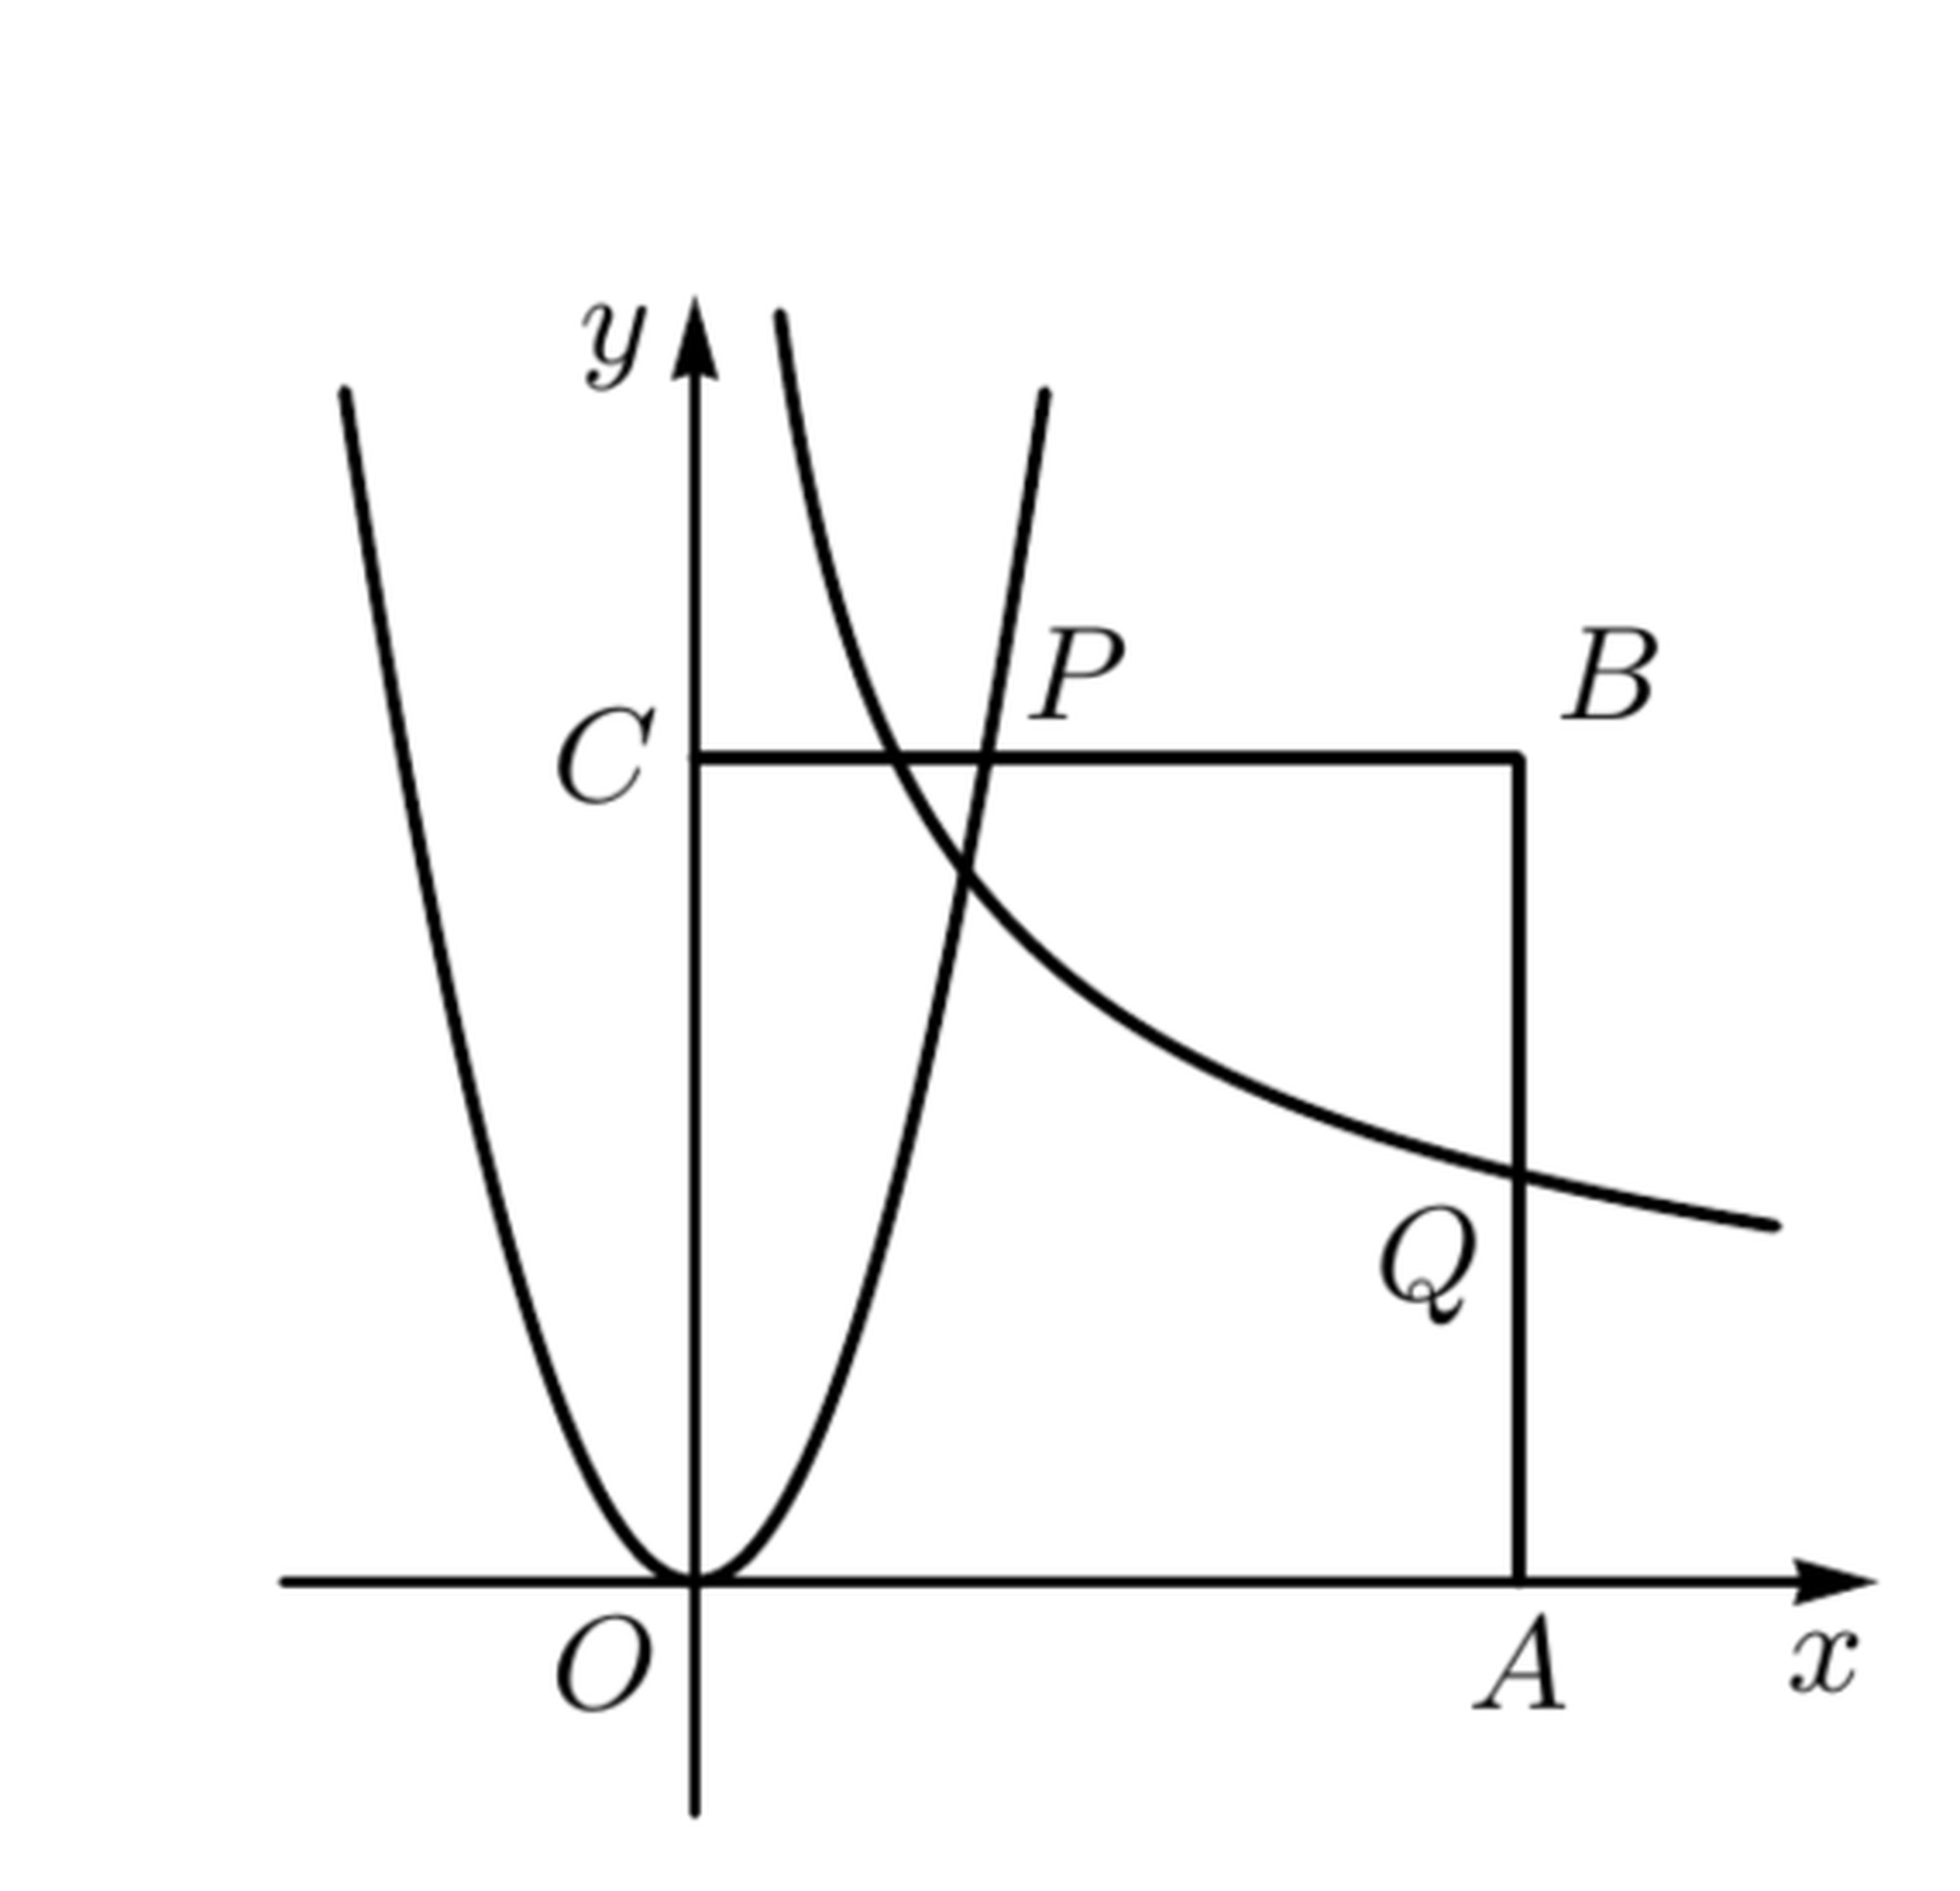
\includegraphics[width=0.40\textwidth]{figures/gao153_q11.png}
\end{center}

\ifanswer
\solbegin
\step{$\lvert AQ\rvert=\dfrac1{\sqrt a}$，$\lvert CP\rvert=\sqrt{\dfrac a5}$，}
\step{于是 $\lvert AQ\rvert+\lvert CP\rvert=\dfrac1{\sqrt a}+\sqrt{\dfrac a5}\geqslant2\sqrt{\dfrac1{\sqrt a}\cdot\sqrt{\dfrac a5}}=\dfrac2{\sqrt[4]{5}}$，}
\step{当且仅当 $\dfrac1{\sqrt a}=\sqrt{\dfrac a5}$，即 $a=\sqrt5$ 时取等号.}
\solend
\fi

% === Q12 === $B\subseteq A$ 带下划线照录、空集 \varnothing；解析 5 行
\item 若集合 $A=\{x\mid1\leqslant x\leqslant100,x\in\Z\}$，集合 $B\subseteq A$，且 $B\ne\varnothing$，记 $W(B)$ 为 $B$ 中元素的最大值与最小值之和，则对所有的 $B$，$W(B)$ 的平均值是\blankline[4.4em].

\ifanswer
\solbegin
\step{对每个非空子集 $B$，令 $B'=\{101-x\mid x\in B\}$，}
\step{则 $W(B')=(101-\min B)+(101-\max B)=202-W(B)$.}
\step{对 $B'$ 再作同样变换即得到 $B$，因此 $B$ 遍历所有非空子集时，}
\step{$B'$ 也恰好遍历所有非空子集.}
\step{设所求平均值为 $m$，则 $m=202-m$，解得 $m=101$.}
\solend
\fi

\end{enumerate}

\bigsec{二、选择题}

\begin{enumerate}
\setcounter{enumi}{12}

% === Q13 === "图像"（像，有亻）照录；解析 2 行，故选 A
\item 设 $a$、$b$ 为常数，若 $0<a<1$，$b>1$，则函数 $y=a^x-b$ 的图像必定不经过\mbox{（\quad）}

\keepwithprev
A. 第一象限\qquad\qquad B. 第二象限\qquad\qquad C. 第三象限\qquad\qquad D. 第四象限

\ifanswer
\solbegin
\step{当 $x>0$ 时，$a^x<1<b$，所以 $y=a^x-b<0$，图像必定不经过第一象限，}
\step{故选 $A$.}
\solend
\fi

% === Q14 === $m\in\Z$、中文弯引号、"图像"照录；解析 3 行，故选 A
\item 已知 $m\in\Z$，则“$m=0$”是“幂函数 $y=x^{m^2-2m-1}$ 的图像与 $x$ 轴及 $y$ 轴均无交点，且关于原点成中心对称”的\mbox{（\quad）}

\keepwithprev
A. 充分不必要条件\qquad\qquad B. 必要不充分条件

C. 充要条件\qquad\qquad D. 既不充分也不必要条件

\ifanswer
\solbegin
\step{图像满足所述条件 $\Leftrightarrow m^2-2m-1$ 为负奇数 $\Leftrightarrow m=0$ 或 $m=2$.}
\step{$m=0$ 能推出所述条件，但所述条件不能推出 $m=0$，因此是充分不必要条件，}
\step{故选 $A$.}
\solend
\fi

% === Q15 === 四选项一行；解析 5 行（跨 03→04 页），故选 D
\item 设 $a>b>1$，$x>1$，则下列不等式正确的是\mbox{（\quad）}

\keepwithprev
A. $a^x<b^x$\qquad B. $x^a<x^b$\qquad C. $\log_a x>\log_b x$\qquad D. $\log_x a>\log_x b$

\ifanswer
\solbegin
\step{$x>1$，幂函数与指数函数的单调性给出 $a^x>b^x$，$x^a>x^b$，A、B 错误.}
\step{$\log_a x=\dfrac{\lg x}{\lg a}<\dfrac{\lg x}{\lg b}=\log_b x$，C 错误.}
\step{对数函数 $y=\log_x t$ 的底数 $x>1$，在 $(0,+\infty)$ 上严格递增，}
\step{所以 $\log_x a>\log_x b$，D 正确.}
\step{故选 $D$.}
\solend
\fi

% === Q16 === $a\in\N$；解析 3 行，故选 C
\item 设 $a\in\N$，则满足不等式 $x^2-a^2x-a^2-1<0$ 的整数 $x$ 的个数不可能是\mbox{（\quad）}

\keepwithprev
A. 1\qquad\qquad B. 50\qquad\qquad C. 100\qquad\qquad D. 2026

\ifanswer
\solbegin
\step{$(x+1)(x-a^2-1)<0\Leftrightarrow-1<x<a^2+1$. 整数解为 $0,1,\cdots,a^2$，共 $a^2+1$ 个.}
\step{$1=0^2+1$，$50=7^2+1$，$2026=45^2+1$，而 $100-1=99$ 不是完全平方数，}
\step{故选 $C$.}
\solend
\fi

\end{enumerate}

\bigsec{三、解答题}

\begin{enumerate}
\setcounter{enumi}{16}

% === Q17 === 补集上划线 \overline{A}、\subseteq 照录；解析 5 行
\item 已知全集 $U=\R$，集合 $A=\{x\mid x^2-x-2\geqslant0\}$，$B=\{x\mid x>-1\}$，$C=\{x\mid a-5<x<a\}$.

(1) 求 $A\cap B$、$A\cup B$；

(2) 若 $\overline{A}\cup C=C$，求实数 $a$ 的取值范围.

\ifanswer
\solbegin
\step{(1) $x^2-x-2=(x+1)(x-2)\geqslant0\Leftrightarrow x\leqslant-1$ 或 $x\geqslant2$，}
\step{所以 $A=(-\infty,-1]\cup[2,+\infty)$，$B=(-1,+\infty)$，}
\step{因此 $A\cap B=[2,+\infty)$，$A\cup B=\R$.}
\step{(2) $\overline{A}=(-1,2)$，于是 $\overline{A}\cup C=C\Leftrightarrow\overline{A}\subseteq C\Leftrightarrow(-1,2)\subseteq(a-5,a)$，}
\step{两区间均为开区间，端点可重合，故 $\begin{cases}a-5\leqslant-1\\a\geqslant2\end{cases}\Leftrightarrow2\leqslant a\leqslant4$.}
\solend
\fi

% === Q18 === 解析 4 行
\item 已知 $a$、$b$、$c$ 都是正数，

(1) 若 $a+b=1$，求证：$\dfrac1a+\dfrac1b\geqslant4$，并指出等号成立的条件；

(2) 若 $a+b+c=1$，求证：三个数 $\dfrac1a$、$\dfrac1b$、$\dfrac1c$ 中至少有一个不小于 3.

\ifanswer
\solbegin
\step{(1) 由 $(a-b)^2\geqslant0$，得 $4ab\leqslant(a+b)^2=1$，所以 $\dfrac1a+\dfrac1b=\dfrac{a+b}{ab}=\dfrac1{ab}\geqslant4$，}
\step{等号成立当且仅当 $a=b$，结合 $a+b=1$，得 $a=b=\dfrac12$.}
\step{(2) 假设三个数 $\dfrac1a$、$\dfrac1b$、$\dfrac1c$ 都小于 3，则 $a>\dfrac13,b>\dfrac13,c>\dfrac13\Rightarrow a+b+c>1$，}
\step{与 $a+b+c=1$ 矛盾，因此三个数中至少有一个不小于 3.}
\solend
\fi

% === Q19 === 题目配图（三版都出）；\needvspace 守卫放 \item 之前；解析 19 行
\needvspace{8cm}
\item 某新建居民小区有一直角三角形绿地，两直角边长分别为 30m 和 40m，打算在其中划出一片区域改造成活动场地，如图所示.

(1) 若划出的区域为正方形，且有两边落在绿地边界上，求此正方形边长；

(2) 若划出的区域为圆形，求圆形区域面积的最大值；

(3) 若划出的区域为矩形（其中至少有一边在边界上），求此矩形面积的最大值.

\begin{center}
% 直角三角形 ABC 绿地示意图取 05 页右上，去粉色水印、去色、4× LANCZOS 放大；三版都出
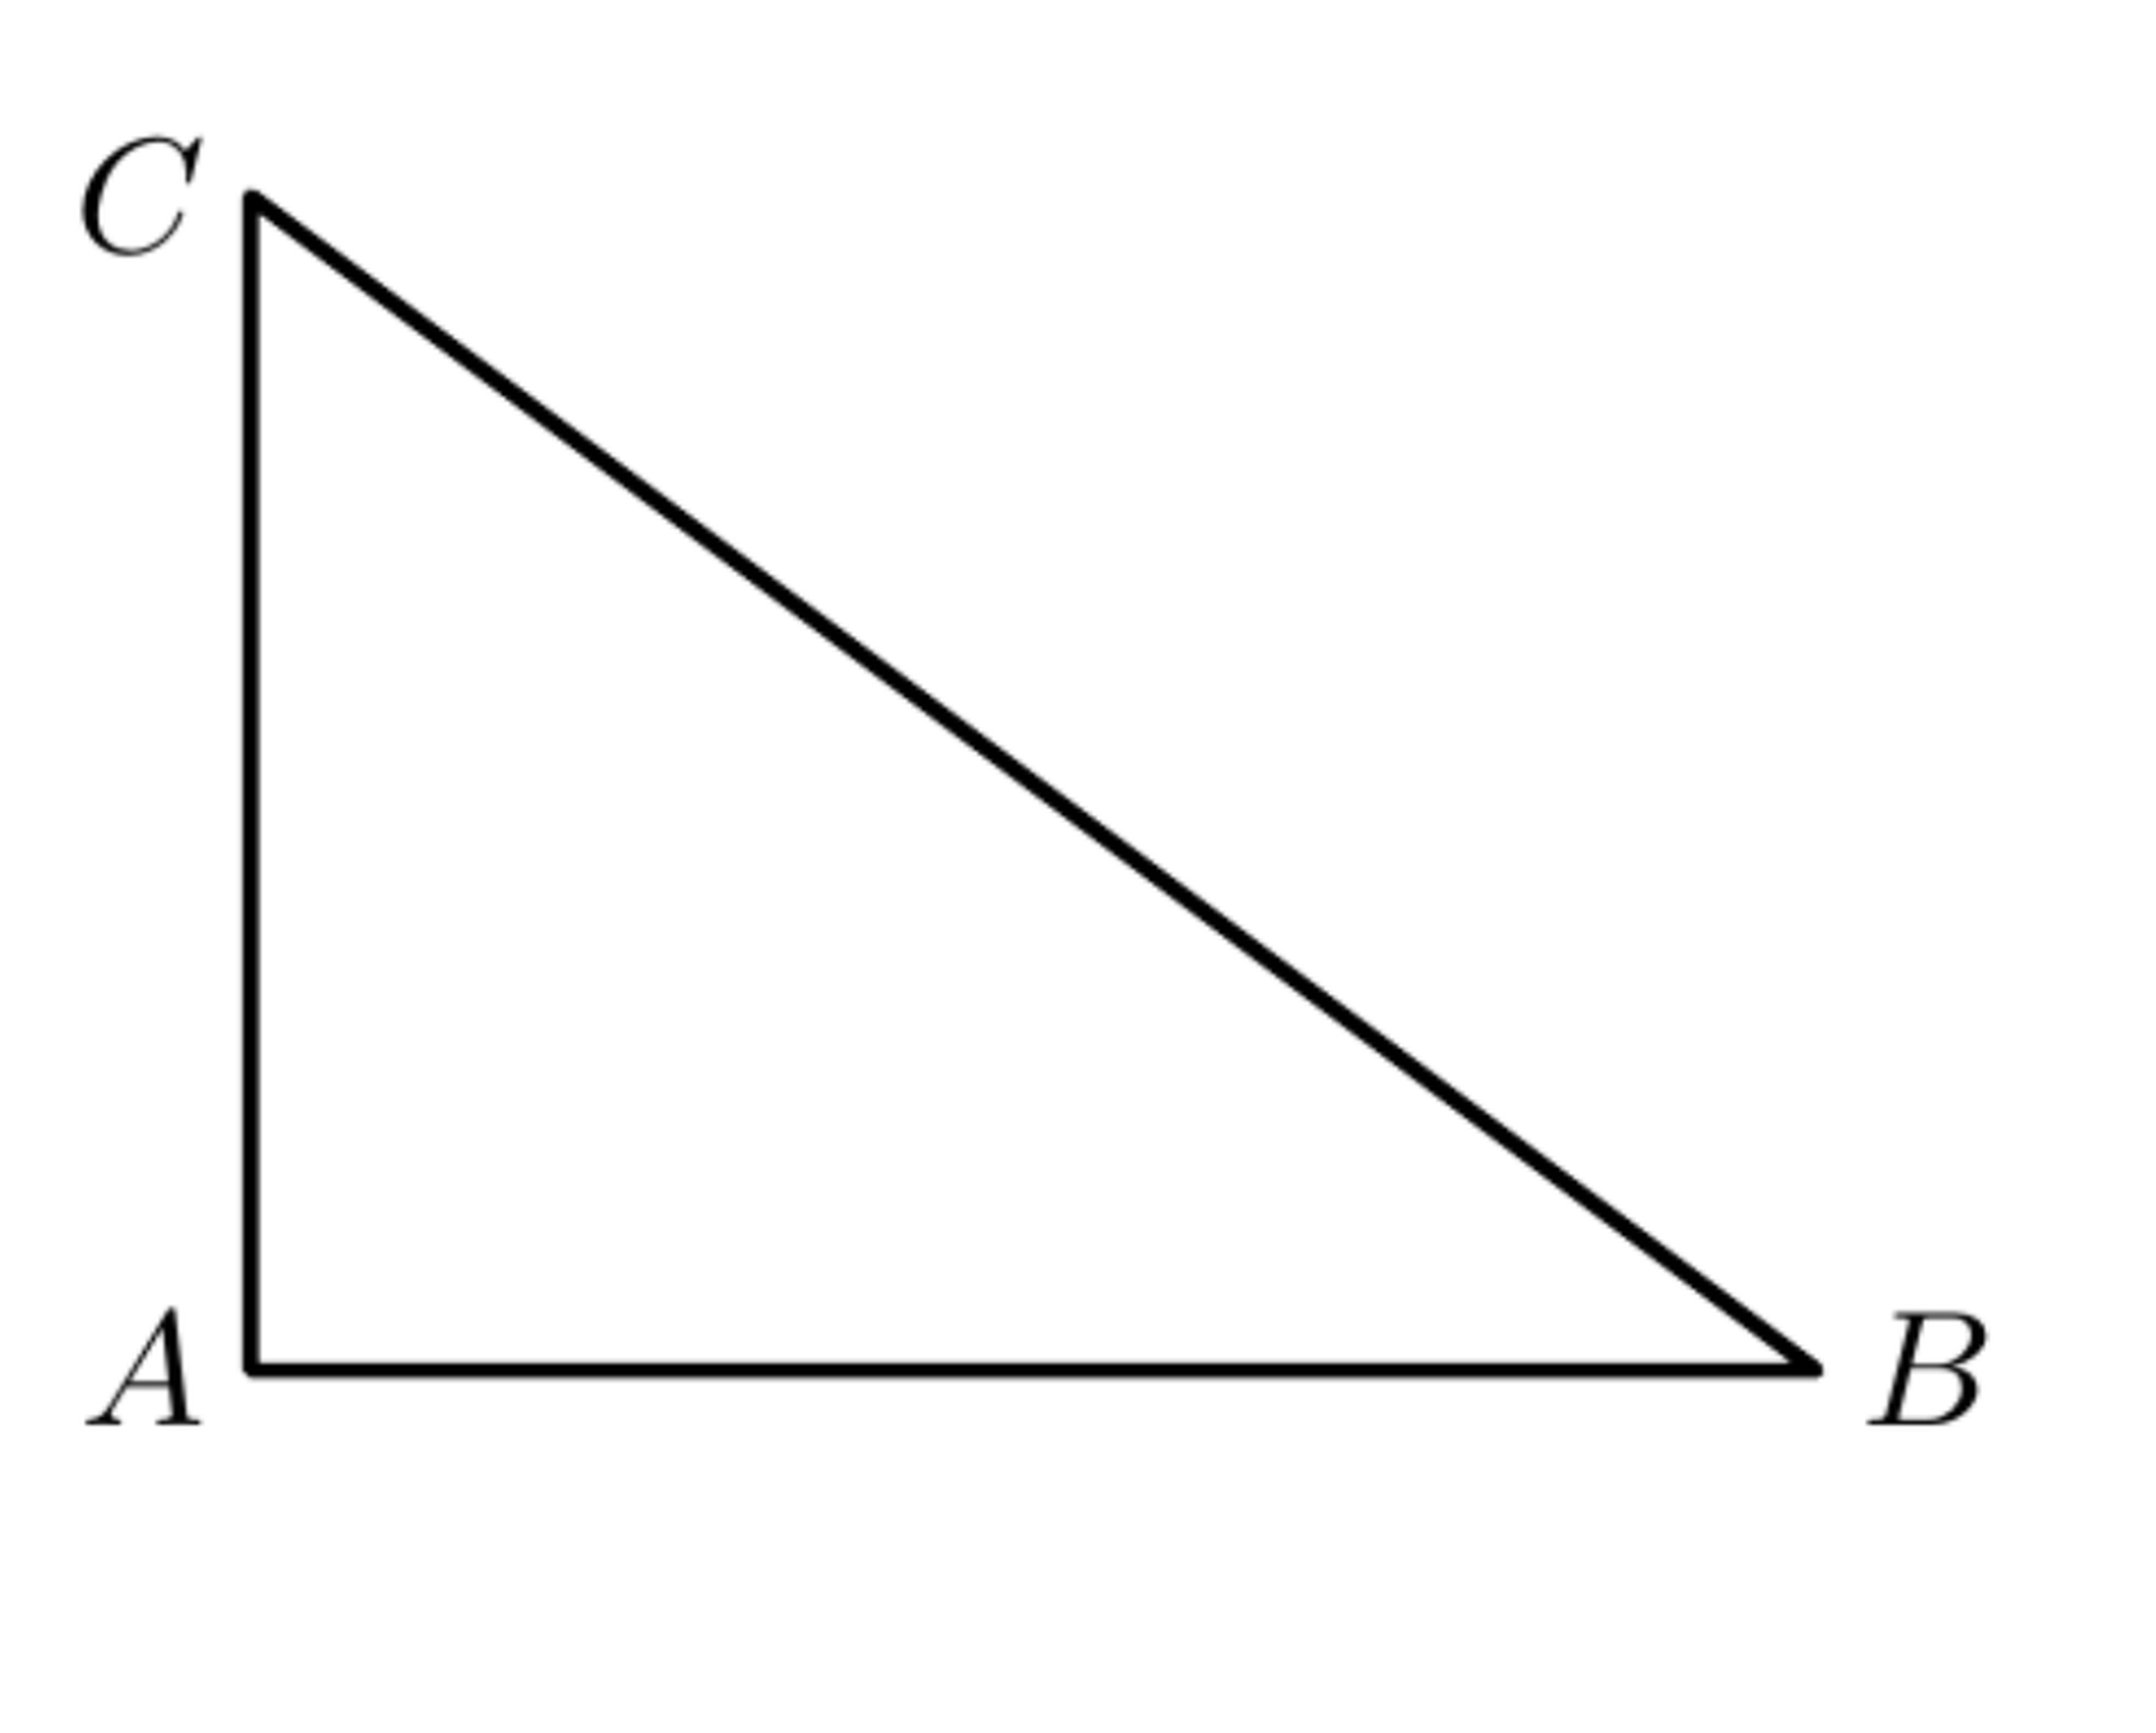
\includegraphics[width=0.34\textwidth]{figures/gao153_q19.png}
\end{center}

\ifanswer
\solbegin
\step{(1) 取 $A(0,0)$、$B(40,0)$、$C(0,30)$，则斜边 $BC$ 所在直线为 $3x+4y=120$.}
\step{正方形落在边界上的两边必分别在两条直角边上.}
\step{设其边长为 $a$m，则对角顶点为 $(a,a)$.}
\step{按题意划出的正方形应尽量大，即对角顶点落在斜边 $BC$ 上，}
\step{因此 $3a+4a=120\Rightarrow a=\dfrac{120}{7}$；}
\step{(2) 斜边长 $BC=\sqrt{30^2+40^2}=50$m，三角形面积为 $600\text{m}^2$.}
\step{设圆的半径为 $r$，圆心到 $AB$、$AC$、$BC$ 的距离分别为 $d_1,d_2,d_3$，}
\step{则三者均不小于 $r$. 连接圆心与三个顶点，}
\step{得 $600=\dfrac12(40d_1+30d_2+50d_3)\geqslant\dfrac12(40+30+50)r=60r$，所以 $r\leqslant10$.}
\step{取三角形的内切圆时等号成立，圆形区域面积的最大值为 $100\pi\text{m}^2$.}
\step{(3) 任取矩形落在绿地边界上的一边，以其所在直线为横轴.}
\step{设相应三角形底边长为 $L$、高为 $H$，则 $LH=1200$.}
\step{取三角形顶点坐标为 $(0,0)$、$(L,0)$、$(p,H)$.}
\step{在高度 $t$ 处，两腰上的点的横坐标分别为 $\dfrac{pt}{H}$、$L+\dfrac{(p-L)t}{H}$，}
\step{因此，高为 $t$ 的矩形，其底边长不超过 $L\left(1-\dfrac tH\right)$，}
\step{面积满足 $S\leqslant Lt\left(1-\dfrac tH\right)=\dfrac LH\left[\dfrac{H^2}{4}-\left(t-\dfrac H2\right)^2\right]\leqslant\dfrac{LH}{4}=300$，}
\step{在原坐标系中，取矩形顶点为 $(0,0)$、$(20,0)$、$(20,15)$、$(0,15)$，}
\step{其中 $3\times20+4\times15=120$，矩形完全位于绿地内，面积为 $300\text{m}^2$，}
\step{达到最大值.}
\solend
\fi

% === Q20 === $g(x)$ 定义照录；解析 14 行
\item 已知 $a>0$ 且 $a\ne1$，设 $f(x)=\log_a(x^2-a^2)$，$g(x)=2\log_a(x-ak)$.

(1) 求函数 $y=f(x)$ 的定义域；

(2) 若 $k=2$，求不等式 $f(x)>g(x)$ 的解集；

(3) 若“存在实数 $x$，使得 $f(x)=g(x)$”为真命题，求实数 $k$ 的取值范围.

\ifanswer
\solbegin
\step{(1) $x^2-a^2>0\Leftrightarrow x<-a$ 或 $x>a$，定义域为 $(-\infty,-a)\cup(a,+\infty)$.}
\step{(2) 两函数均有意义时，$x>2a$，且 $g(x)=\log_a(x-2a)^2$.}
\step{当 $a>1$ 时，$f(x)>g(x)\Leftrightarrow x^2-a^2>(x-2a)^2\Leftrightarrow x>\dfrac{5a}{4}$，}
\step{结合 $x>2a$，解集为 $(2a,+\infty)$.}
\step{当 $0<a<1$ 时，$f(x)>g(x)\Leftrightarrow x^2-a^2<(x-2a)^2\Leftrightarrow x<\dfrac{5a}{4}$，}
\step{与 $x>2a$ 矛盾，解集为 $\varnothing$.}
\step{(3) 在 $x^2-a^2>0$ 且 $x-ak>0$ 的条件下，}
\step{$f(x)=g(x)\Leftrightarrow x^2-a^2=(x-ak)^2\Leftrightarrow2akx=a^2(1+k^2)$，}
\step{当 $k=0$ 时，上式不成立；}
\step{当 $k\ne0$ 时，$x=\dfrac{a(1+k^2)}{2k}$，}
\step{于是 $x-ak=\dfrac{a(1-k^2)}{2k}>0\Leftrightarrow k<-1$ 或 $0<k<1$，}
\step{对上述 $k$，所取的 $x$ 同时满足 $x^2-a^2=(x-ak)^2>0$，}
\step{两函数均有意义且函数值相等.}
\step{因此，$k$ 的取值范围为 $(-\infty,-1)\cup(0,1)$.}
\solend
\fi

% === Q21 === 中文弯引号、复杂式照录；解析 23 行（跨 08→09 页）
\item 若实数 $x$、$y$、$m$ 满足 $\lvert x-m\rvert<\lvert y-m\rvert$，则称 $x$ 比 $y$ 接近 $m$.

(1) 若 $2x$ 比 $x-2$ 更接近 1，求实数 $x$ 的取值范围；

(2) 若 $x$ 比 $y$ 接近 $m$，证明：“$x>y$” 的充要条件是 “$x+y<2m$”；

(3) 已知 $x>0$，$y>0$ 且 $x\ne y$. 设 $p=\dfrac{x^2+y^2}{xy}$，若对于任意的 $x$、$y$，命题 “$p$ 比 $p^2-3p+4$ 接近 $m$” 恒成立，求实数 $m$ 的取值范围.

\ifanswer
\solbegin
\step{(1) $\lvert2x-1\rvert<\lvert x-3\rvert\Leftrightarrow(2x-1)^2<(x-3)^2\Leftrightarrow(x+2)(3x-4)<0$，}
\step{解得 $-2<x<\dfrac43$，实数 $x$ 的取值范围为 $\left(-2,\dfrac43\right)$.}
\step{(2) 因为 $x$ 比 $y$ 接近 $m$，所以 $\lvert x-m\rvert<\lvert y-m\rvert$，则 $\lvert x-m\rvert^2<\lvert y-m\rvert^2$，}
\step{即 $(x-m)^2<(y-m)^2$，即 $(x-m)^2-(y-m)^2<0$，}
\step{即得 $(x-y)(x+y-2m)<0$，}
\step{则由 $x+y<2m$，得 $x+y-2m<0$，}
\step{故 $x-y>0$，即 $x>y$，充分性成立；}
\step{当 $x>y$ 时，$x-y>0$，结合 $(x-y)(x+y-2m)<0$，得 $x+y-2m<0$，}
\step{即 $x+y<2m$，必要性成立；}
\step{故“$x>y$” 的充要条件是 “$x+y<2m$”；}
\step{(3) $x>0$，$y>0$ 且 $x\ne y$. 则 $p=\dfrac{x^2+y^2}{xy}=\dfrac xy+\dfrac yx>2\sqrt{\dfrac xy\cdot\dfrac yx}=2$，}
\step{由于对于任意的 $x$、$y$，命题 “$p$ 比 $p^2-3p+4$ 接近 $m$” 恒成立，}
\step{故 $\lvert p-m\rvert<\lvert(p^2-3p+4)-m\rvert$ 对 $\forall p>2$ 恒成立，}
\step{即得 $(p-m)^2<(p^2-3p+4-m)^2$，}
\step{即 $(p^2-3p+4-m)^2-(p-m)^2>0$，}
\step{得 $(p^2-4p+4)(p^2-2p+4-2m)>0$，}
\step{即 $(p-2)^2(p^2-2p+4-2m)>0$，由于 $p>2$，故 $(p-2)^2>0$，}
\step{故 $p^2-2p+4-2m>0$ 对 $\forall p>2$ 恒成立，}
\step{即 $2m<p^2-2p+4$ 对 $\forall p>2$ 恒成立，}
\step{由于 $p^2-2p+4=(p-1)^2+3$，此时 $p^2-2p+4$ 在 $(2,+\infty)$ 上严格增，}
\step{故 $(p-1)^2+3>(2-1)^2+3=4$，故 $2m\leqslant4$，解得 $m\leqslant2$，}
\step{即实数 $m$ 的取值范围是 $(-\infty,2]$.}
\solend
\fi

\end{enumerate}

\end{document}
"
% 紧凑版：xelatex "\def\iscompact{1}% 高一153_闵行中学文绮中学_期中.tex
%   —— 高一上数学"2026-2027 年闵行中学文绮中学高一上期中"（试卷版/答案版/紧凑版）
% 试卷版：xelatex 高一153_闵行中学文绮中学_期中.tex
% 答案版：xelatex "\def\isanswer{1}\input{高一153_闵行中学文绮中学_期中.tex}"
% 紧凑版：xelatex "\def\iscompact{1}\input{高一153_闵行中学文绮中学_期中.tex}"
%
% ① 原始材料：微信公众号"魔都数学加油站"文章，连载"27学年高一153"，原文标题
% "27学年高一153——2026-2027年上海市闵行中学文绮中学高一上期中"；
% 原文链接：https://mp.weixin.qq.com/s/rEtS-92cDR6JKgY2b5DRfg 。
% 正文为 9 张 PNG 页（01/02/06/07/08/09 为 2560×3620，03/04/05 为 4762×6735，
% 同一篇各页分辨率混排，逐页按各自分辨率裁图核对，别按预览比例换算裁框）。
% 体例：讲评版——填空 3—12（10 题）、选择 13—16（4 题）、解答 17—21（5 题），
% 共 19 题，自第 3 题起编；**全 19 题均印【解析】**（逐题核实，见 ② ②）。
% 题目、答案、解析均据原图转录；卷面粉红色水印"魔都数学加油站"及公众号页脚未录入。
% 全卷插图清单（逐页通读 9 页确认）：2 幅，均为题目配图、三版都出——
%   · Q11 正方形 OABC 曲线图（02 页右下：$y=5x^2$ 与 $y=x^{-\frac12}$ 两条曲线、
%     坐标轴、O/A/B/C/P/Q、正方形），裁 figures/gao153_q11.png；
%   · Q19 直角三角形 ABC 绿地示意图（05 页右上，直角在 A），
%     裁 figures/gao153_q19.png；
%   两图均去粉色水印、去色、4× LANCZOS 放大；Q11 图左上角题干残字"函"已裁白。
%   其余各页逐页确认无其它题目配图、无解析内配图、无表格；09 页下半仅水印、无正文。
%
% 卷首标题：原卷印作"2026-2027 年闵行中学文绮中学高一上期中"，年份区间按全稿惯例排 en dash；
% 原卷卷面未印副标题，本稿按同期中卷知识模块口径补出"集合与常用逻辑用语、不等式、函数"。
%
% ② 与原卷的排版差异：
%   ① 原文从第 3 题起，本稿保留原题号；共 19 题三节，解答题 5 题到 21；
%   ② 全 19 题均印【解析】、用 \solbegin…\solend，无只印【答案】或答案印括号内的题；
%      四道选择题答案在解析末句"故选 A／A／D／C"（Q13—Q16，逐个放大复核）、
%      括号 \mbox{（\quad）} 留空、不另提 \ans{}；答案版【答案】/【解析】标记数
%      = 19 = 全卷题数；
%   ③ 原卷卷面未印副标题，本稿按知识模块口径补出；
%   ④ 原卷填空横线按全稿惯例排 \blankline[4.4em]；选择题括号排 \mbox{（\quad）}、
%      四道选择题的选项段前按惯例各加 \keepwithprev；解答题不留作答区、不加
%      \anspace（原卷为讲评版，109—113 起全稿不用 \anspace）；
%   ⑤ 数集：Q3"$x\in R$"、Q5"解集为 R"、Q10"$x\in N$"、Q12"$x\in Z$"与
%      "$m\in Z$"、Q14"$m\in Z$"、Q16"$a\in N$"、Q17"全集 $U=R$"、
%      Q19 无、Q21 无——原卷印斜体或正体粗体 R/N/Z，按全稿惯例归一
%      \R／\N／\Z；绝对值排 \lvert…\rvert（Q5、Q11、Q21），集合描述竖线排 \mid
%      （Q3、Q10、Q17、Q20），不等号按全稿惯例排 \leqslant／\geqslant；
%      补集照原卷上划线排 \overline{A}（Q17 题干 (2)＋解析 (2)）；
%      空集 \varnothing（Q12 题干、Q20 解析 (2)）；子集 3 处均印带下划线 ⊆、
%      照录 \subseteq（Q10 $A\subseteq U$、Q12 $B\subseteq A$、Q17 $(-1,2)\subseteq(a-5,a)$），
%      本卷无单线 \subset 用例；
%   ⑥ 判别式：逐页通读 9 页，本卷无一元二次判别式 Δ/△ 算式，故无 Δ/△ 混用可照录；
%      Q11 图里有几何正方形 OABC（非三角形符号），无 △ABC 用例；
%   ⑦ 中文弯引号照录：Q14"$m=0$"与"幂函数…关于原点成中心对称"、
%      Q20"存在实数 $x$，使得 $f(x)=g(x)$"、Q21"$x>y$"与"$x+y<2m$"、
%      "$p$ 比 $p^2-3p+4$ 接近 $m$"（引号外留空格按原卷）；
%      注释里一律 ASCII 引号；数学式内 CJK 用 \text{}；
%   ⑧ "图像／图象"逐处放大核：全卷 3 处均印"图像"（像，有亻）——
%      Q13 题干与解析、Q14 题干与解析；Q19 题干写"如图所示"（非"图像"），
%      逐处照录未统一；子题标号 (1)(2)(3) 半角括号照录；圈数字本卷无用例；
%   ⑨ 半角逗号在数学组之间是全稿惯例、非笔误，逐处照录（Q3 $x\in R$、
%      Q10 $a_1,a_2$、Q19 $A(0,0)$、$d_1,d_2,d_3$、Q21 $a>\frac13,b>\frac13$ 等）；
%      行末西文句点 ASCII `.`；行中全角逗号／顿号照录（Q19"30m 和 40m"、
%      Q21"实数 $x$、$y$、$m$"）；
%   ⑩ 复杂式照录别简化：Q3 $y=x^{-2}$、Q11 $y=x^{-\frac12}$ 与
%      $\frac{2}{\sqrt[4]{5}}$、Q8 $\frac{2b}{a+1-b}$、Q9 cases 块、
%      Q10 $525=5\times105$、Q16 $a^2+1$、Q19 $S\leqslant Lt(1-\frac tH)$
%      与 $L+\frac{(p-L)t}{H}$、Q20 $2akx=a^2(1+k^2)$ 与 $\frac{a(1+k^2)}{2k}$、
%      Q21 $(p^2-4p+4)(p^2-2p+4-2m)>0$；
%      \left…\right 不得拆到不同 $…$ 组（Q17 $\left\{x\mid\cdots\right\}$、
%      Q19 $\left[\frac{H^2}{4}-\left(t-\frac H2\right)^2\right]$、
%      Q21 $\left(-2,\frac43\right)$ 等）；cases 块一律 \begin{cases}…\end{cases}；
%   ⑪ 一条 \step = 原卷解析的一个印刷行，cases 块整体算一个印刷行；别并折行、
%      别拆行。Q10 六行、Q19 十九行、Q20 十四行、Q21 二十二行均按印刷行逐条断，
%      不丢行；
%   ⑫ 配图：Q11／Q19 题目配图（三版都出）放 \item 内题干之后 \begin{center}，
%      各用 \needvspace{8cm} 守卫把整块推走，**守卫放在 \item 之前**
%      （见 高一145 Q14/Q20 成例与切页审计 B 类坑）；
%   ⑬ 原卷解析内无红色"法一／法二"之类小标题，故本卷无 \stepm；红色水印
%      "魔都数学加油站"不录入；
%   ⑭ 跨页续印按题合并：见 ⑥；
%
% ③ 行数复核：一条 \step = 原卷解析的一个印刷行，cases 块作一个印刷行计。
%   逐题数（主会话逐页核对定稿）：Q3：1；Q4：2；Q5：2；Q6：2；Q7：1；
%   Q8：1；Q9：2；Q10：6；Q11：3；Q12：5；Q13：2；Q14：3；Q15：5；
%   Q16：3；Q17：5；Q18：4；Q19：19；Q20：14；Q21：22。
%   合计 102 条 \step（本卷无 \stepm），与原卷逐题印刷行相等。全卷 19 题
%   均设 \solbegin…\solend，答案版【答案】/【解析】标记数 = 19 = 全卷题数。
%
% ④ 判别式／子集符号结论（逐处放大原图照录、不得统一，主会话像素级复核）：
%   判别式：逐页通读 9 页，本卷无一元二次判别式算式（Q7 用韦达定理、
%      Q16 用因式分解、Q20 用对数方程，均不写 Δ/△），故无 Δ/△ 混用可照录
%      （"高 \Delta／扁 \triangle"口径备查，参照 高一142／151／152 头注）；
%      本卷无几何三角形符号用例。
%   子集：Q10 题干"$A\subseteq U$"、Q12 题干"$B\subseteq A$"、Q17 解析 (2)
%      "$(-1,2)\subseteq(a-5,a)$"共 3 处，逐处放大确认均印带下划线 ⊆、
%      照录 \subseteq；本卷未见单线 ⊂（\subset）之对应处。
%      补集上划线 \overline{A}（Q17）、空集 \varnothing（Q12 题干、Q20 解析 (2)）；
%      数集 \R／\N／\Z 归一见 ② ⑤。
%
% ⑤ 存疑照录（放大原图确认，照录未改、正文对应处另有 % 注）：
%   1. Q3 集合 $B=\{(x,y)\mid y=x^{-2},x\in\R\}$ 原卷题干径写 $x\in\R$
%      （$x=0$ 处无意义），解析自行注明 $x\ne0$，照录未改。
%   2. Q10 解析"$U$ 中共有 $525=5\times105$ 个连续整数"与尾行
%      "取 $U$ 中除以 5 余 1 或 2 的全部元素及元素 5"逐字照录（放大 02 页
%      /tmp/gao153/z/zoom/q10_pick.png 确认是"元素 5"，非"元素 9"）。
%   3. Q11 第二个函数原卷印 $y=x^{-\frac12}$（负二分之一次幂，非 $x^2$），
%      放大 02 页 /tmp/gao153/z/zoom/q11_exp.png 确认，照录未改；
%      $|AQ|=\frac1{\sqrt a}$ 与之自洽。
%   4. Q19 (3) 解析"在高度 $t$ 处，两腰上的点的横坐标分别为 $\frac{pt}{H}$、
%      $L+\frac{(p-L)t}{H}$"，放大 06 页确认，照录未简化。
%   5. Q20 (2) 解析"$g(x)=\log_a(x-2a)^2$"（真数整体平方），
%      与 $g(x)=2\log_a(x-ak)$ 在 $k=2$ 时一致，照录未改。
%   6. Q21 (3) 解析"得 $(p^2-4p+4)(p^2-2p+4-2m)>0$"与
%      "故 $(p-1)^2+3>(2-1)^2+3=4$，故 $2m\leqslant4$"照录未改
%      （放大 09 页 /tmp/gao153/z/zoom/q21_factor.png 确认）。
%   7. "图像／图象"全卷 3 处均印"图像"（像，有亻）逐处照录；
%      本卷无判别式 Δ/△ 用例（见 ④）。
%   全卷除此 7 类外未发现其它笔误／自相矛盾处；19 题均印【解析】、
%   无只印【答案】或答案印括号内的题（见 ② ②）。
%
% ⑥ 跨页续印按题合并说明（逐页核实定稿）：Q3—Q5 题干＋解析在 01 页；
%   Q6—Q8 题干＋解析在 01 页下半（Q8 解析续 02 页顶）；Q9 题干＋解析、
%   Q10 题干＋解析首 2 行在 02 页上半，Q10 解析余 4 行在 02 页下半；
%   Q11 题干＋配图＋解析、Q12 题干＋解析 5 行在 02 页下半—03 页上半；
%   "二、选择题"标题在 03 页中部；Q13 题干＋选项＋解析在 03 页下半；
%   Q14 题干＋选项＋解析、Q15 题干＋选项＋解析首行在 03 页下半—04 页顶；
%   Q15 解析余 4 行、Q16 题干＋选项＋解析在 04 页上半；"三、解答题"
%   标题在 04 页下半；Q17 题干＋两问＋解析 5 行在 04 页下半—05 页顶；
%   Q18 题干＋两问＋解析 4 行、Q19 题干（含配图）＋三问在 05 页；
%   Q19 解析 (1)(2) 9 行在 05 页下半，解析 (3) 前 5 行在 06 页上半、
%   余 4 行在 06 页下半；Q20 题干＋三问在 06 页下半，解析 (1)(2)(3)
%   前 6 行在 07 页上半、(3) 余 8 行在 07 页下半；Q21 题干＋三问在
%   07 页末，解析 (1)(2) 10 行在 08 页上半—下半，解析 (3) 前 4 行在
%   08 页下半、余 9 行续 09 页上半，末行"即实数 $m$ 的取值范围是
%   $(-\infty,2]$"为全卷收尾（09 页下半仅水印、无正文）。
%   本稿按题连排，不丢行、不并折行；全卷末题为第 21 题，无附加题节。
%
\documentclass[a4paper,11pt]{article}
\usepackage{common}

\begin{document}

\examtitlest[3]{2026--2027 年闵行中学文绮中学高一上期中}{集合与常用逻辑用语、不等式、函数}

\bigsec{一、填空题}

\begin{enumerate}
\setcounter{enumi}{2}

% === Q3 === 集合描述竖线 \mid；$y=x^{-2}$ 照录；解析 1 行
\item 已知 $A=\{(x,y)\mid y=x^3,x\in\R\}$，$B=\{(x,y)\mid y=x^{-2},x\in\R\}$，则 $A\cap B=$\blankline[4.4em].

\ifanswer
\solbegin
\step{$x^3=x^{-2}\ (x\ne0)\Leftrightarrow x^5=1\Leftrightarrow x=1$，此时 $y=1$，所以 $A\cap B=\{(1,1)\}$.}
\solend
\fi

% === Q4 === 解析 2 行
\item 若关于 $x$ 的不等式 $\dfrac{x-a}{x+1}>0$ 的解集为 $(-\infty,-1)\cup(4,+\infty)$，则实数 $a=$\blankline[4.4em].

\ifanswer
\solbegin
\step{关于 $x$ 的不等式 $\dfrac{x-a}{x+1}>0$ 即 $(x+1)(x-a)>0$.}
\step{再由它的解集为 $(-\infty,-1)\cup(4,+\infty)$，得 $-1$ 和 4 是 $(x+1)(x-a)=0$ 的两个实数根，故 $a=4$.}
\solend
\fi

% === Q5 === 绝对值 \lvert…\rvert；解析 2 行
\item 若关于 $x$ 的不等式 $\lvert x+1\rvert+\lvert x-2\rvert>m$ 的解集为 $\R$，则实数 $m$ 的取值范围是\blankline[4.4em].

\ifanswer
\solbegin
\step{$\lvert x+1\rvert+\lvert x-2\rvert\geqslant\lvert(x+1)-(x-2)\rvert=3$，当且仅当 $-1\leqslant x\leqslant2$ 时取等号，}
\step{因此 $m<3$.}
\solend
\fi

% === Q6 === 解析 2 行
\item 已知指数函数 $y=a^x$（$a>1$）在区间 $[-1,1]$ 上的最大值比最小值大 $\dfrac32$，则实数 $a=$\blankline[4.4em].

\ifanswer
\solbegin
\step{$a>1$，指数函数在 $[-1,1]$ 上严格增，故 $a-\dfrac1a=\dfrac32\Leftrightarrow(a-2)(2a+1)=0$.}
\step{结合 $a>1$，得 $a=2$.}
\solend
\fi

% === Q7 === 韦达定理；解析 1 行
\item 已知关于 $x$ 的一元二次方程 $x^2+px+2p=0$ 的两个实数根分别为 $x_1$、$x_2$，且 $(x_1+1)(x_2+1)=0$，则 $p=$\blankline[4.4em].

\ifanswer
\solbegin
\step{$0=(x_1+1)(x_2+1)=x_1x_2+x_1+x_2+1=2p-p+1=p+1\Rightarrow p=-1$.}
\solend
\fi

% === Q8 === 换底公式；解析 1 行
\item 已知 $10^a=3$，$\lg5=b$，则 $\log_6 25=$\blankline[4.4em]（用关于 $a,b$ 的关系式表示）.

\ifanswer
\solbegin
\step{$\lg3=a$，$\lg2=1-b$，所以 $\log_6 25=\dfrac{\lg25}{\lg6}=\dfrac{2b}{a+1-b}$.}
\solend
\fi

% === Q9 === cases 块整体算一个印刷行；解析 2 行
\item 已知 $A=[2,5]$，若对任意 $x\in A$，总有 $\dfrac{k}{x}\in A$，则正数 $k=$\blankline[4.4em].

\ifanswer
\solbegin
\step{$k>0$，当 $x\in[2,5]$ 时，$\dfrac{k}{x}$ 的取值范围为 $\left[\dfrac k5,\dfrac k2\right]$，}
\step{因此 $\begin{cases}\dfrac k5\geqslant2\\\dfrac k2\leqslant5\end{cases}\Leftrightarrow10\leqslant k\leqslant10\Leftrightarrow k=10$.}
\solend
\fi

% === Q10 === $A\subseteq U$ 带下划线照录；解析 6 行
\item 已知集合 $U=\{x\mid4\leqslant x\leqslant528,x\in\N\}$，$A=\{a_1,a_2,a_3,\cdots,a_n\}$，且 $A\subseteq U$. 如果集合 $A$ 中的任意两个不同元素之和都不能被 5 整除，则正整数 $n$ 的最大值为\blankline[4.4em].

\ifanswer
\solbegin
\step{$U$ 中共有 $525=5\times105$ 个连续整数，按除以 5 的余数分成五类，}
\step{每类均有 105 个元素.}
\step{余数为 1,4 的两类不能同时选取，余数为 2,3 的两类也不能同时选取，}
\step{余数为 0 的一类最多选 1 个，因此 $n\leqslant105+105+1=211$.}
\step{取 $U$ 中除以 5 余 1 或 2 的全部元素及元素 5，}% 放大 02 页确认是「元素 5」（非 9），照录未改（见 ⑤ 2）
\step{任意两个不同元素之和均不能被 5 整除，此时 $n=211$，最大值为 211.}
\solend
\fi

% === Q11 === 题目配图（三版都出）；\needvspace 守卫放 \item 之前；$y=x^{-\frac12}$ 照录；解析 3 行
\needvspace{8cm}
\item 如图，已知正方形 $OABC$，其中 $OA=a$（$a>1$），函数 $y=5x^2$ 交 $BC$ 于点 $P$，函数 $y=x^{-\frac12}$ 交 $AB$ 于点 $Q$，当 $\lvert AQ\rvert+\lvert CP\rvert$ 最小时，$a$ 的值为\blankline[4.4em].

\begin{center}
% 正方形 OABC 与两条曲线图取 02 页右下，去粉色水印、去色、4× LANCZOS 放大；三版都出
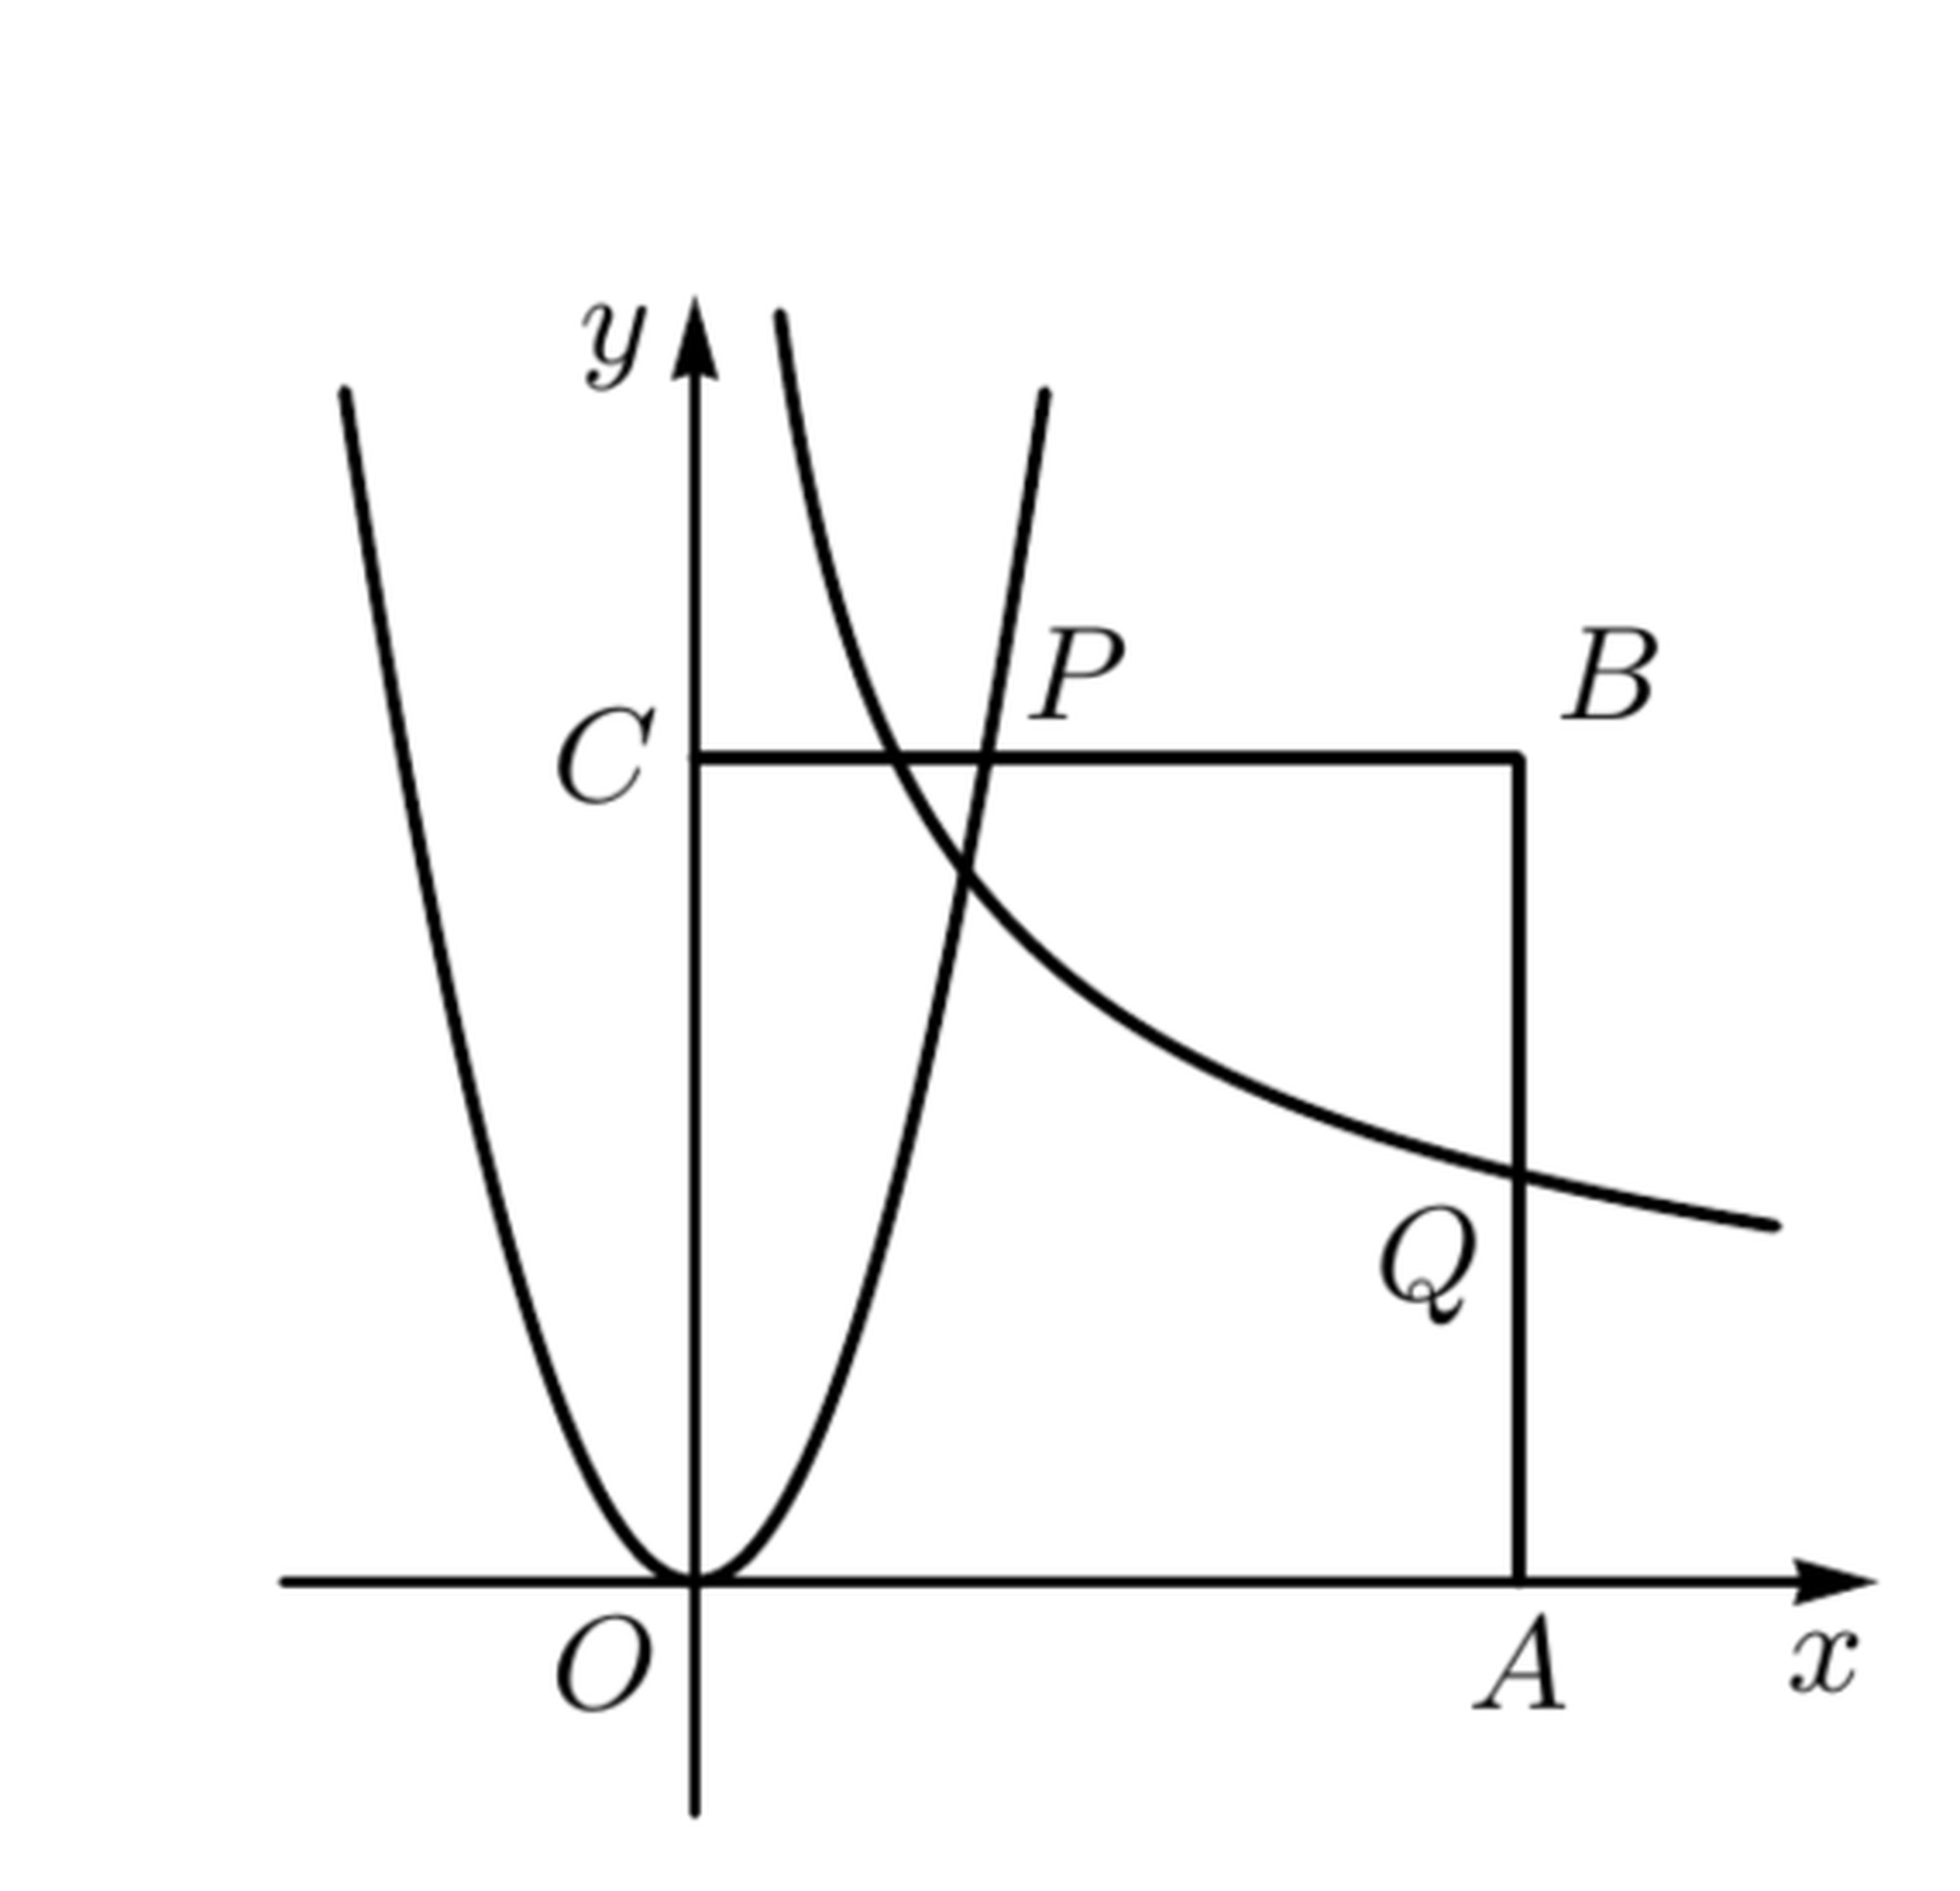
\includegraphics[width=0.40\textwidth]{figures/gao153_q11.png}
\end{center}

\ifanswer
\solbegin
\step{$\lvert AQ\rvert=\dfrac1{\sqrt a}$，$\lvert CP\rvert=\sqrt{\dfrac a5}$，}
\step{于是 $\lvert AQ\rvert+\lvert CP\rvert=\dfrac1{\sqrt a}+\sqrt{\dfrac a5}\geqslant2\sqrt{\dfrac1{\sqrt a}\cdot\sqrt{\dfrac a5}}=\dfrac2{\sqrt[4]{5}}$，}
\step{当且仅当 $\dfrac1{\sqrt a}=\sqrt{\dfrac a5}$，即 $a=\sqrt5$ 时取等号.}
\solend
\fi

% === Q12 === $B\subseteq A$ 带下划线照录、空集 \varnothing；解析 5 行
\item 若集合 $A=\{x\mid1\leqslant x\leqslant100,x\in\Z\}$，集合 $B\subseteq A$，且 $B\ne\varnothing$，记 $W(B)$ 为 $B$ 中元素的最大值与最小值之和，则对所有的 $B$，$W(B)$ 的平均值是\blankline[4.4em].

\ifanswer
\solbegin
\step{对每个非空子集 $B$，令 $B'=\{101-x\mid x\in B\}$，}
\step{则 $W(B')=(101-\min B)+(101-\max B)=202-W(B)$.}
\step{对 $B'$ 再作同样变换即得到 $B$，因此 $B$ 遍历所有非空子集时，}
\step{$B'$ 也恰好遍历所有非空子集.}
\step{设所求平均值为 $m$，则 $m=202-m$，解得 $m=101$.}
\solend
\fi

\end{enumerate}

\bigsec{二、选择题}

\begin{enumerate}
\setcounter{enumi}{12}

% === Q13 === "图像"（像，有亻）照录；解析 2 行，故选 A
\item 设 $a$、$b$ 为常数，若 $0<a<1$，$b>1$，则函数 $y=a^x-b$ 的图像必定不经过\mbox{（\quad）}

\keepwithprev
A. 第一象限\qquad\qquad B. 第二象限\qquad\qquad C. 第三象限\qquad\qquad D. 第四象限

\ifanswer
\solbegin
\step{当 $x>0$ 时，$a^x<1<b$，所以 $y=a^x-b<0$，图像必定不经过第一象限，}
\step{故选 $A$.}
\solend
\fi

% === Q14 === $m\in\Z$、中文弯引号、"图像"照录；解析 3 行，故选 A
\item 已知 $m\in\Z$，则“$m=0$”是“幂函数 $y=x^{m^2-2m-1}$ 的图像与 $x$ 轴及 $y$ 轴均无交点，且关于原点成中心对称”的\mbox{（\quad）}

\keepwithprev
A. 充分不必要条件\qquad\qquad B. 必要不充分条件

C. 充要条件\qquad\qquad D. 既不充分也不必要条件

\ifanswer
\solbegin
\step{图像满足所述条件 $\Leftrightarrow m^2-2m-1$ 为负奇数 $\Leftrightarrow m=0$ 或 $m=2$.}
\step{$m=0$ 能推出所述条件，但所述条件不能推出 $m=0$，因此是充分不必要条件，}
\step{故选 $A$.}
\solend
\fi

% === Q15 === 四选项一行；解析 5 行（跨 03→04 页），故选 D
\item 设 $a>b>1$，$x>1$，则下列不等式正确的是\mbox{（\quad）}

\keepwithprev
A. $a^x<b^x$\qquad B. $x^a<x^b$\qquad C. $\log_a x>\log_b x$\qquad D. $\log_x a>\log_x b$

\ifanswer
\solbegin
\step{$x>1$，幂函数与指数函数的单调性给出 $a^x>b^x$，$x^a>x^b$，A、B 错误.}
\step{$\log_a x=\dfrac{\lg x}{\lg a}<\dfrac{\lg x}{\lg b}=\log_b x$，C 错误.}
\step{对数函数 $y=\log_x t$ 的底数 $x>1$，在 $(0,+\infty)$ 上严格递增，}
\step{所以 $\log_x a>\log_x b$，D 正确.}
\step{故选 $D$.}
\solend
\fi

% === Q16 === $a\in\N$；解析 3 行，故选 C
\item 设 $a\in\N$，则满足不等式 $x^2-a^2x-a^2-1<0$ 的整数 $x$ 的个数不可能是\mbox{（\quad）}

\keepwithprev
A. 1\qquad\qquad B. 50\qquad\qquad C. 100\qquad\qquad D. 2026

\ifanswer
\solbegin
\step{$(x+1)(x-a^2-1)<0\Leftrightarrow-1<x<a^2+1$. 整数解为 $0,1,\cdots,a^2$，共 $a^2+1$ 个.}
\step{$1=0^2+1$，$50=7^2+1$，$2026=45^2+1$，而 $100-1=99$ 不是完全平方数，}
\step{故选 $C$.}
\solend
\fi

\end{enumerate}

\bigsec{三、解答题}

\begin{enumerate}
\setcounter{enumi}{16}

% === Q17 === 补集上划线 \overline{A}、\subseteq 照录；解析 5 行
\item 已知全集 $U=\R$，集合 $A=\{x\mid x^2-x-2\geqslant0\}$，$B=\{x\mid x>-1\}$，$C=\{x\mid a-5<x<a\}$.

(1) 求 $A\cap B$、$A\cup B$；

(2) 若 $\overline{A}\cup C=C$，求实数 $a$ 的取值范围.

\ifanswer
\solbegin
\step{(1) $x^2-x-2=(x+1)(x-2)\geqslant0\Leftrightarrow x\leqslant-1$ 或 $x\geqslant2$，}
\step{所以 $A=(-\infty,-1]\cup[2,+\infty)$，$B=(-1,+\infty)$，}
\step{因此 $A\cap B=[2,+\infty)$，$A\cup B=\R$.}
\step{(2) $\overline{A}=(-1,2)$，于是 $\overline{A}\cup C=C\Leftrightarrow\overline{A}\subseteq C\Leftrightarrow(-1,2)\subseteq(a-5,a)$，}
\step{两区间均为开区间，端点可重合，故 $\begin{cases}a-5\leqslant-1\\a\geqslant2\end{cases}\Leftrightarrow2\leqslant a\leqslant4$.}
\solend
\fi

% === Q18 === 解析 4 行
\item 已知 $a$、$b$、$c$ 都是正数，

(1) 若 $a+b=1$，求证：$\dfrac1a+\dfrac1b\geqslant4$，并指出等号成立的条件；

(2) 若 $a+b+c=1$，求证：三个数 $\dfrac1a$、$\dfrac1b$、$\dfrac1c$ 中至少有一个不小于 3.

\ifanswer
\solbegin
\step{(1) 由 $(a-b)^2\geqslant0$，得 $4ab\leqslant(a+b)^2=1$，所以 $\dfrac1a+\dfrac1b=\dfrac{a+b}{ab}=\dfrac1{ab}\geqslant4$，}
\step{等号成立当且仅当 $a=b$，结合 $a+b=1$，得 $a=b=\dfrac12$.}
\step{(2) 假设三个数 $\dfrac1a$、$\dfrac1b$、$\dfrac1c$ 都小于 3，则 $a>\dfrac13,b>\dfrac13,c>\dfrac13\Rightarrow a+b+c>1$，}
\step{与 $a+b+c=1$ 矛盾，因此三个数中至少有一个不小于 3.}
\solend
\fi

% === Q19 === 题目配图（三版都出）；\needvspace 守卫放 \item 之前；解析 19 行
\needvspace{8cm}
\item 某新建居民小区有一直角三角形绿地，两直角边长分别为 30m 和 40m，打算在其中划出一片区域改造成活动场地，如图所示.

(1) 若划出的区域为正方形，且有两边落在绿地边界上，求此正方形边长；

(2) 若划出的区域为圆形，求圆形区域面积的最大值；

(3) 若划出的区域为矩形（其中至少有一边在边界上），求此矩形面积的最大值.

\begin{center}
% 直角三角形 ABC 绿地示意图取 05 页右上，去粉色水印、去色、4× LANCZOS 放大；三版都出
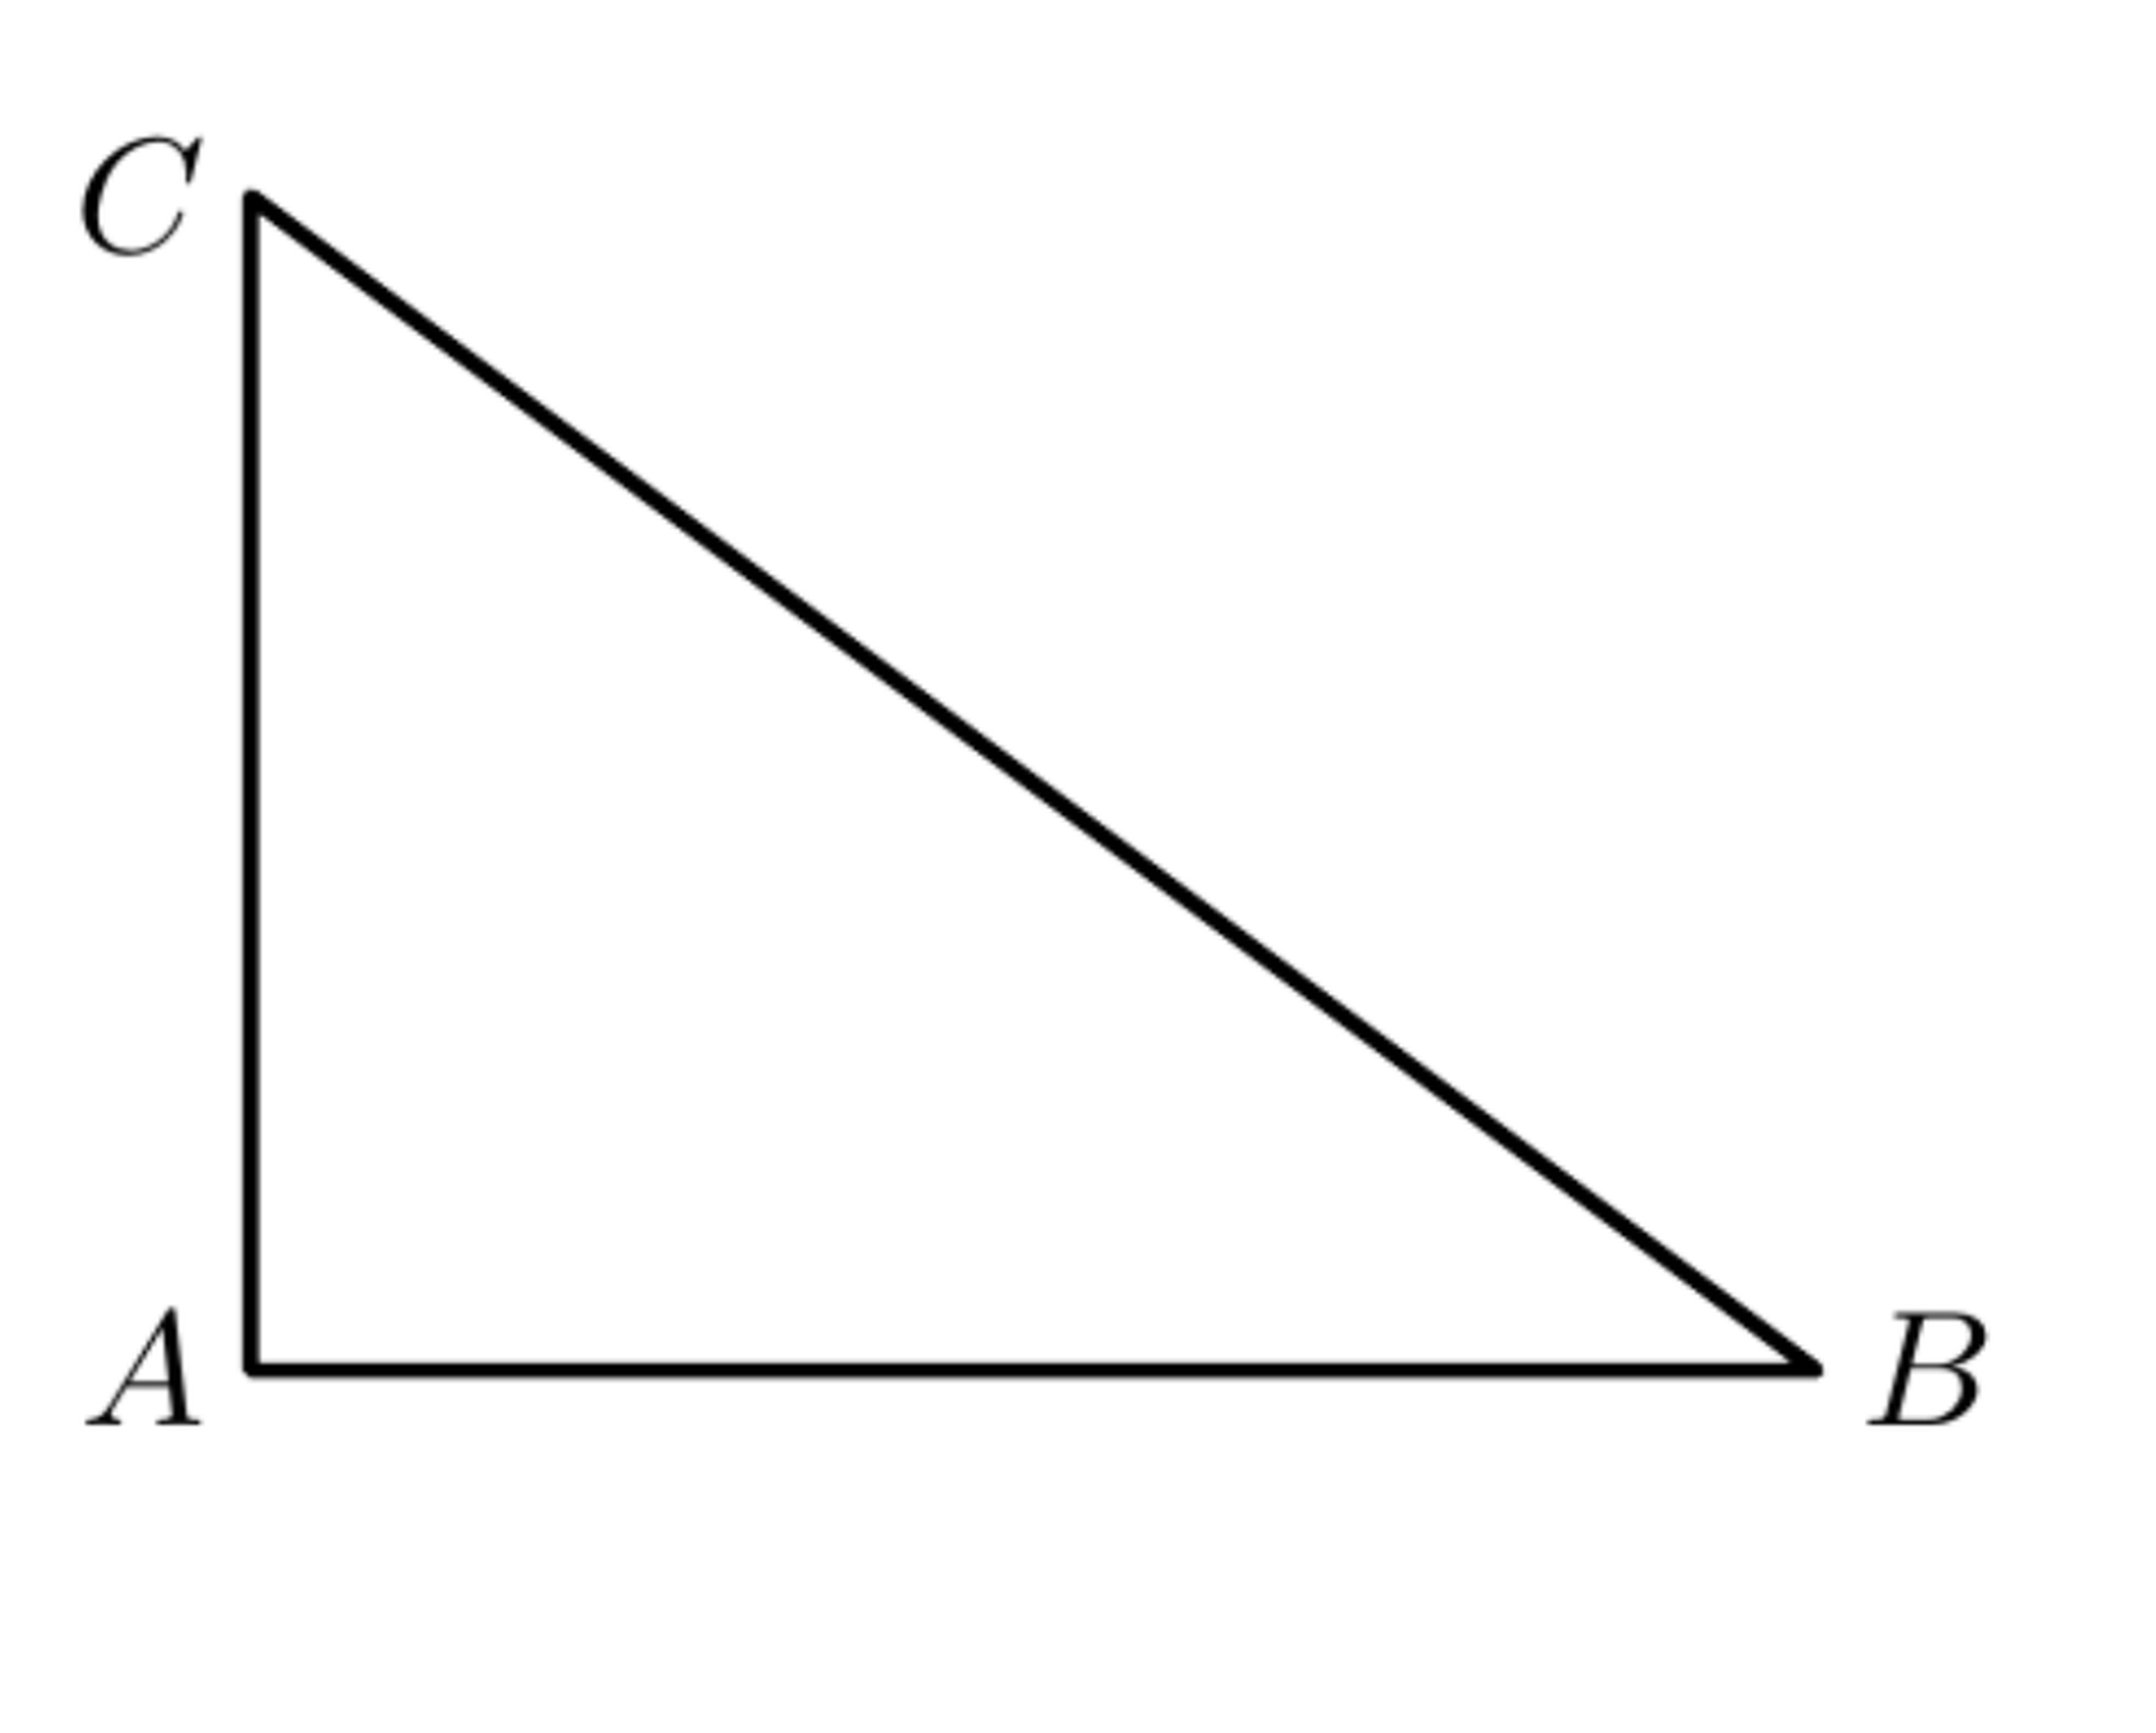
\includegraphics[width=0.34\textwidth]{figures/gao153_q19.png}
\end{center}

\ifanswer
\solbegin
\step{(1) 取 $A(0,0)$、$B(40,0)$、$C(0,30)$，则斜边 $BC$ 所在直线为 $3x+4y=120$.}
\step{正方形落在边界上的两边必分别在两条直角边上.}
\step{设其边长为 $a$m，则对角顶点为 $(a,a)$.}
\step{按题意划出的正方形应尽量大，即对角顶点落在斜边 $BC$ 上，}
\step{因此 $3a+4a=120\Rightarrow a=\dfrac{120}{7}$；}
\step{(2) 斜边长 $BC=\sqrt{30^2+40^2}=50$m，三角形面积为 $600\text{m}^2$.}
\step{设圆的半径为 $r$，圆心到 $AB$、$AC$、$BC$ 的距离分别为 $d_1,d_2,d_3$，}
\step{则三者均不小于 $r$. 连接圆心与三个顶点，}
\step{得 $600=\dfrac12(40d_1+30d_2+50d_3)\geqslant\dfrac12(40+30+50)r=60r$，所以 $r\leqslant10$.}
\step{取三角形的内切圆时等号成立，圆形区域面积的最大值为 $100\pi\text{m}^2$.}
\step{(3) 任取矩形落在绿地边界上的一边，以其所在直线为横轴.}
\step{设相应三角形底边长为 $L$、高为 $H$，则 $LH=1200$.}
\step{取三角形顶点坐标为 $(0,0)$、$(L,0)$、$(p,H)$.}
\step{在高度 $t$ 处，两腰上的点的横坐标分别为 $\dfrac{pt}{H}$、$L+\dfrac{(p-L)t}{H}$，}
\step{因此，高为 $t$ 的矩形，其底边长不超过 $L\left(1-\dfrac tH\right)$，}
\step{面积满足 $S\leqslant Lt\left(1-\dfrac tH\right)=\dfrac LH\left[\dfrac{H^2}{4}-\left(t-\dfrac H2\right)^2\right]\leqslant\dfrac{LH}{4}=300$，}
\step{在原坐标系中，取矩形顶点为 $(0,0)$、$(20,0)$、$(20,15)$、$(0,15)$，}
\step{其中 $3\times20+4\times15=120$，矩形完全位于绿地内，面积为 $300\text{m}^2$，}
\step{达到最大值.}
\solend
\fi

% === Q20 === $g(x)$ 定义照录；解析 14 行
\item 已知 $a>0$ 且 $a\ne1$，设 $f(x)=\log_a(x^2-a^2)$，$g(x)=2\log_a(x-ak)$.

(1) 求函数 $y=f(x)$ 的定义域；

(2) 若 $k=2$，求不等式 $f(x)>g(x)$ 的解集；

(3) 若“存在实数 $x$，使得 $f(x)=g(x)$”为真命题，求实数 $k$ 的取值范围.

\ifanswer
\solbegin
\step{(1) $x^2-a^2>0\Leftrightarrow x<-a$ 或 $x>a$，定义域为 $(-\infty,-a)\cup(a,+\infty)$.}
\step{(2) 两函数均有意义时，$x>2a$，且 $g(x)=\log_a(x-2a)^2$.}
\step{当 $a>1$ 时，$f(x)>g(x)\Leftrightarrow x^2-a^2>(x-2a)^2\Leftrightarrow x>\dfrac{5a}{4}$，}
\step{结合 $x>2a$，解集为 $(2a,+\infty)$.}
\step{当 $0<a<1$ 时，$f(x)>g(x)\Leftrightarrow x^2-a^2<(x-2a)^2\Leftrightarrow x<\dfrac{5a}{4}$，}
\step{与 $x>2a$ 矛盾，解集为 $\varnothing$.}
\step{(3) 在 $x^2-a^2>0$ 且 $x-ak>0$ 的条件下，}
\step{$f(x)=g(x)\Leftrightarrow x^2-a^2=(x-ak)^2\Leftrightarrow2akx=a^2(1+k^2)$，}
\step{当 $k=0$ 时，上式不成立；}
\step{当 $k\ne0$ 时，$x=\dfrac{a(1+k^2)}{2k}$，}
\step{于是 $x-ak=\dfrac{a(1-k^2)}{2k}>0\Leftrightarrow k<-1$ 或 $0<k<1$，}
\step{对上述 $k$，所取的 $x$ 同时满足 $x^2-a^2=(x-ak)^2>0$，}
\step{两函数均有意义且函数值相等.}
\step{因此，$k$ 的取值范围为 $(-\infty,-1)\cup(0,1)$.}
\solend
\fi

% === Q21 === 中文弯引号、复杂式照录；解析 23 行（跨 08→09 页）
\item 若实数 $x$、$y$、$m$ 满足 $\lvert x-m\rvert<\lvert y-m\rvert$，则称 $x$ 比 $y$ 接近 $m$.

(1) 若 $2x$ 比 $x-2$ 更接近 1，求实数 $x$ 的取值范围；

(2) 若 $x$ 比 $y$ 接近 $m$，证明：“$x>y$” 的充要条件是 “$x+y<2m$”；

(3) 已知 $x>0$，$y>0$ 且 $x\ne y$. 设 $p=\dfrac{x^2+y^2}{xy}$，若对于任意的 $x$、$y$，命题 “$p$ 比 $p^2-3p+4$ 接近 $m$” 恒成立，求实数 $m$ 的取值范围.

\ifanswer
\solbegin
\step{(1) $\lvert2x-1\rvert<\lvert x-3\rvert\Leftrightarrow(2x-1)^2<(x-3)^2\Leftrightarrow(x+2)(3x-4)<0$，}
\step{解得 $-2<x<\dfrac43$，实数 $x$ 的取值范围为 $\left(-2,\dfrac43\right)$.}
\step{(2) 因为 $x$ 比 $y$ 接近 $m$，所以 $\lvert x-m\rvert<\lvert y-m\rvert$，则 $\lvert x-m\rvert^2<\lvert y-m\rvert^2$，}
\step{即 $(x-m)^2<(y-m)^2$，即 $(x-m)^2-(y-m)^2<0$，}
\step{即得 $(x-y)(x+y-2m)<0$，}
\step{则由 $x+y<2m$，得 $x+y-2m<0$，}
\step{故 $x-y>0$，即 $x>y$，充分性成立；}
\step{当 $x>y$ 时，$x-y>0$，结合 $(x-y)(x+y-2m)<0$，得 $x+y-2m<0$，}
\step{即 $x+y<2m$，必要性成立；}
\step{故“$x>y$” 的充要条件是 “$x+y<2m$”；}
\step{(3) $x>0$，$y>0$ 且 $x\ne y$. 则 $p=\dfrac{x^2+y^2}{xy}=\dfrac xy+\dfrac yx>2\sqrt{\dfrac xy\cdot\dfrac yx}=2$，}
\step{由于对于任意的 $x$、$y$，命题 “$p$ 比 $p^2-3p+4$ 接近 $m$” 恒成立，}
\step{故 $\lvert p-m\rvert<\lvert(p^2-3p+4)-m\rvert$ 对 $\forall p>2$ 恒成立，}
\step{即得 $(p-m)^2<(p^2-3p+4-m)^2$，}
\step{即 $(p^2-3p+4-m)^2-(p-m)^2>0$，}
\step{得 $(p^2-4p+4)(p^2-2p+4-2m)>0$，}
\step{即 $(p-2)^2(p^2-2p+4-2m)>0$，由于 $p>2$，故 $(p-2)^2>0$，}
\step{故 $p^2-2p+4-2m>0$ 对 $\forall p>2$ 恒成立，}
\step{即 $2m<p^2-2p+4$ 对 $\forall p>2$ 恒成立，}
\step{由于 $p^2-2p+4=(p-1)^2+3$，此时 $p^2-2p+4$ 在 $(2,+\infty)$ 上严格增，}
\step{故 $(p-1)^2+3>(2-1)^2+3=4$，故 $2m\leqslant4$，解得 $m\leqslant2$，}
\step{即实数 $m$ 的取值范围是 $(-\infty,2]$.}
\solend
\fi

\end{enumerate}

\end{document}
"
%
% ① 原始材料：微信公众号"魔都数学加油站"文章，连载"27学年高一153"，原文标题
% "27学年高一153——2026-2027年上海市闵行中学文绮中学高一上期中"；
% 原文链接：https://mp.weixin.qq.com/s/rEtS-92cDR6JKgY2b5DRfg 。
% 正文为 9 张 PNG 页（01/02/06/07/08/09 为 2560×3620，03/04/05 为 4762×6735，
% 同一篇各页分辨率混排，逐页按各自分辨率裁图核对，别按预览比例换算裁框）。
% 体例：讲评版——填空 3—12（10 题）、选择 13—16（4 题）、解答 17—21（5 题），
% 共 19 题，自第 3 题起编；**全 19 题均印【解析】**（逐题核实，见 ② ②）。
% 题目、答案、解析均据原图转录；卷面粉红色水印"魔都数学加油站"及公众号页脚未录入。
% 全卷插图清单（逐页通读 9 页确认）：2 幅，均为题目配图、三版都出——
%   · Q11 正方形 OABC 曲线图（02 页右下：$y=5x^2$ 与 $y=x^{-\frac12}$ 两条曲线、
%     坐标轴、O/A/B/C/P/Q、正方形），裁 figures/gao153_q11.png；
%   · Q19 直角三角形 ABC 绿地示意图（05 页右上，直角在 A），
%     裁 figures/gao153_q19.png；
%   两图均去粉色水印、去色、4× LANCZOS 放大；Q11 图左上角题干残字"函"已裁白。
%   其余各页逐页确认无其它题目配图、无解析内配图、无表格；09 页下半仅水印、无正文。
%
% 卷首标题：原卷印作"2026-2027 年闵行中学文绮中学高一上期中"，年份区间按全稿惯例排 en dash；
% 原卷卷面未印副标题，本稿按同期中卷知识模块口径补出"集合与常用逻辑用语、不等式、函数"。
%
% ② 与原卷的排版差异：
%   ① 原文从第 3 题起，本稿保留原题号；共 19 题三节，解答题 5 题到 21；
%   ② 全 19 题均印【解析】、用 \solbegin…\solend，无只印【答案】或答案印括号内的题；
%      四道选择题答案在解析末句"故选 A／A／D／C"（Q13—Q16，逐个放大复核）、
%      括号 \mbox{（\quad）} 留空、不另提 \ans{}；答案版【答案】/【解析】标记数
%      = 19 = 全卷题数；
%   ③ 原卷卷面未印副标题，本稿按知识模块口径补出；
%   ④ 原卷填空横线按全稿惯例排 \blankline[4.4em]；选择题括号排 \mbox{（\quad）}、
%      四道选择题的选项段前按惯例各加 \keepwithprev；解答题不留作答区、不加
%      \anspace（原卷为讲评版，109—113 起全稿不用 \anspace）；
%   ⑤ 数集：Q3"$x\in R$"、Q5"解集为 R"、Q10"$x\in N$"、Q12"$x\in Z$"与
%      "$m\in Z$"、Q14"$m\in Z$"、Q16"$a\in N$"、Q17"全集 $U=R$"、
%      Q19 无、Q21 无——原卷印斜体或正体粗体 R/N/Z，按全稿惯例归一
%      \R／\N／\Z；绝对值排 \lvert…\rvert（Q5、Q11、Q21），集合描述竖线排 \mid
%      （Q3、Q10、Q17、Q20），不等号按全稿惯例排 \leqslant／\geqslant；
%      补集照原卷上划线排 \overline{A}（Q17 题干 (2)＋解析 (2)）；
%      空集 \varnothing（Q12 题干、Q20 解析 (2)）；子集 3 处均印带下划线 ⊆、
%      照录 \subseteq（Q10 $A\subseteq U$、Q12 $B\subseteq A$、Q17 $(-1,2)\subseteq(a-5,a)$），
%      本卷无单线 \subset 用例；
%   ⑥ 判别式：逐页通读 9 页，本卷无一元二次判别式 Δ/△ 算式，故无 Δ/△ 混用可照录；
%      Q11 图里有几何正方形 OABC（非三角形符号），无 △ABC 用例；
%   ⑦ 中文弯引号照录：Q14"$m=0$"与"幂函数…关于原点成中心对称"、
%      Q20"存在实数 $x$，使得 $f(x)=g(x)$"、Q21"$x>y$"与"$x+y<2m$"、
%      "$p$ 比 $p^2-3p+4$ 接近 $m$"（引号外留空格按原卷）；
%      注释里一律 ASCII 引号；数学式内 CJK 用 \text{}；
%   ⑧ "图像／图象"逐处放大核：全卷 3 处均印"图像"（像，有亻）——
%      Q13 题干与解析、Q14 题干与解析；Q19 题干写"如图所示"（非"图像"），
%      逐处照录未统一；子题标号 (1)(2)(3) 半角括号照录；圈数字本卷无用例；
%   ⑨ 半角逗号在数学组之间是全稿惯例、非笔误，逐处照录（Q3 $x\in R$、
%      Q10 $a_1,a_2$、Q19 $A(0,0)$、$d_1,d_2,d_3$、Q21 $a>\frac13,b>\frac13$ 等）；
%      行末西文句点 ASCII `.`；行中全角逗号／顿号照录（Q19"30m 和 40m"、
%      Q21"实数 $x$、$y$、$m$"）；
%   ⑩ 复杂式照录别简化：Q3 $y=x^{-2}$、Q11 $y=x^{-\frac12}$ 与
%      $\frac{2}{\sqrt[4]{5}}$、Q8 $\frac{2b}{a+1-b}$、Q9 cases 块、
%      Q10 $525=5\times105$、Q16 $a^2+1$、Q19 $S\leqslant Lt(1-\frac tH)$
%      与 $L+\frac{(p-L)t}{H}$、Q20 $2akx=a^2(1+k^2)$ 与 $\frac{a(1+k^2)}{2k}$、
%      Q21 $(p^2-4p+4)(p^2-2p+4-2m)>0$；
%      \left…\right 不得拆到不同 $…$ 组（Q17 $\left\{x\mid\cdots\right\}$、
%      Q19 $\left[\frac{H^2}{4}-\left(t-\frac H2\right)^2\right]$、
%      Q21 $\left(-2,\frac43\right)$ 等）；cases 块一律 \begin{cases}…\end{cases}；
%   ⑪ 一条 \step = 原卷解析的一个印刷行，cases 块整体算一个印刷行；别并折行、
%      别拆行。Q10 六行、Q19 十九行、Q20 十四行、Q21 二十二行均按印刷行逐条断，
%      不丢行；
%   ⑫ 配图：Q11／Q19 题目配图（三版都出）放 \item 内题干之后 \begin{center}，
%      各用 \needvspace{8cm} 守卫把整块推走，**守卫放在 \item 之前**
%      （见 高一145 Q14/Q20 成例与切页审计 B 类坑）；
%   ⑬ 原卷解析内无红色"法一／法二"之类小标题，故本卷无 \stepm；红色水印
%      "魔都数学加油站"不录入；
%   ⑭ 跨页续印按题合并：见 ⑥；
%
% ③ 行数复核：一条 \step = 原卷解析的一个印刷行，cases 块作一个印刷行计。
%   逐题数（主会话逐页核对定稿）：Q3：1；Q4：2；Q5：2；Q6：2；Q7：1；
%   Q8：1；Q9：2；Q10：6；Q11：3；Q12：5；Q13：2；Q14：3；Q15：5；
%   Q16：3；Q17：5；Q18：4；Q19：19；Q20：14；Q21：22。
%   合计 102 条 \step（本卷无 \stepm），与原卷逐题印刷行相等。全卷 19 题
%   均设 \solbegin…\solend，答案版【答案】/【解析】标记数 = 19 = 全卷题数。
%
% ④ 判别式／子集符号结论（逐处放大原图照录、不得统一，主会话像素级复核）：
%   判别式：逐页通读 9 页，本卷无一元二次判别式算式（Q7 用韦达定理、
%      Q16 用因式分解、Q20 用对数方程，均不写 Δ/△），故无 Δ/△ 混用可照录
%      （"高 \Delta／扁 \triangle"口径备查，参照 高一142／151／152 头注）；
%      本卷无几何三角形符号用例。
%   子集：Q10 题干"$A\subseteq U$"、Q12 题干"$B\subseteq A$"、Q17 解析 (2)
%      "$(-1,2)\subseteq(a-5,a)$"共 3 处，逐处放大确认均印带下划线 ⊆、
%      照录 \subseteq；本卷未见单线 ⊂（\subset）之对应处。
%      补集上划线 \overline{A}（Q17）、空集 \varnothing（Q12 题干、Q20 解析 (2)）；
%      数集 \R／\N／\Z 归一见 ② ⑤。
%
% ⑤ 存疑照录（放大原图确认，照录未改、正文对应处另有 % 注）：
%   1. Q3 集合 $B=\{(x,y)\mid y=x^{-2},x\in\R\}$ 原卷题干径写 $x\in\R$
%      （$x=0$ 处无意义），解析自行注明 $x\ne0$，照录未改。
%   2. Q10 解析"$U$ 中共有 $525=5\times105$ 个连续整数"与尾行
%      "取 $U$ 中除以 5 余 1 或 2 的全部元素及元素 5"逐字照录（放大 02 页
%      /tmp/gao153/z/zoom/q10_pick.png 确认是"元素 5"，非"元素 9"）。
%   3. Q11 第二个函数原卷印 $y=x^{-\frac12}$（负二分之一次幂，非 $x^2$），
%      放大 02 页 /tmp/gao153/z/zoom/q11_exp.png 确认，照录未改；
%      $|AQ|=\frac1{\sqrt a}$ 与之自洽。
%   4. Q19 (3) 解析"在高度 $t$ 处，两腰上的点的横坐标分别为 $\frac{pt}{H}$、
%      $L+\frac{(p-L)t}{H}$"，放大 06 页确认，照录未简化。
%   5. Q20 (2) 解析"$g(x)=\log_a(x-2a)^2$"（真数整体平方），
%      与 $g(x)=2\log_a(x-ak)$ 在 $k=2$ 时一致，照录未改。
%   6. Q21 (3) 解析"得 $(p^2-4p+4)(p^2-2p+4-2m)>0$"与
%      "故 $(p-1)^2+3>(2-1)^2+3=4$，故 $2m\leqslant4$"照录未改
%      （放大 09 页 /tmp/gao153/z/zoom/q21_factor.png 确认）。
%   7. "图像／图象"全卷 3 处均印"图像"（像，有亻）逐处照录；
%      本卷无判别式 Δ/△ 用例（见 ④）。
%   全卷除此 7 类外未发现其它笔误／自相矛盾处；19 题均印【解析】、
%   无只印【答案】或答案印括号内的题（见 ② ②）。
%
% ⑥ 跨页续印按题合并说明（逐页核实定稿）：Q3—Q5 题干＋解析在 01 页；
%   Q6—Q8 题干＋解析在 01 页下半（Q8 解析续 02 页顶）；Q9 题干＋解析、
%   Q10 题干＋解析首 2 行在 02 页上半，Q10 解析余 4 行在 02 页下半；
%   Q11 题干＋配图＋解析、Q12 题干＋解析 5 行在 02 页下半—03 页上半；
%   "二、选择题"标题在 03 页中部；Q13 题干＋选项＋解析在 03 页下半；
%   Q14 题干＋选项＋解析、Q15 题干＋选项＋解析首行在 03 页下半—04 页顶；
%   Q15 解析余 4 行、Q16 题干＋选项＋解析在 04 页上半；"三、解答题"
%   标题在 04 页下半；Q17 题干＋两问＋解析 5 行在 04 页下半—05 页顶；
%   Q18 题干＋两问＋解析 4 行、Q19 题干（含配图）＋三问在 05 页；
%   Q19 解析 (1)(2) 9 行在 05 页下半，解析 (3) 前 5 行在 06 页上半、
%   余 4 行在 06 页下半；Q20 题干＋三问在 06 页下半，解析 (1)(2)(3)
%   前 6 行在 07 页上半、(3) 余 8 行在 07 页下半；Q21 题干＋三问在
%   07 页末，解析 (1)(2) 10 行在 08 页上半—下半，解析 (3) 前 4 行在
%   08 页下半、余 9 行续 09 页上半，末行"即实数 $m$ 的取值范围是
%   $(-\infty,2]$"为全卷收尾（09 页下半仅水印、无正文）。
%   本稿按题连排，不丢行、不并折行；全卷末题为第 21 题，无附加题节。
%
\documentclass[a4paper,11pt]{article}
\usepackage{common}

\begin{document}

\examtitlest[3]{2026--2027 年闵行中学文绮中学高一上期中}{集合与常用逻辑用语、不等式、函数}

\bigsec{一、填空题}

\begin{enumerate}
\setcounter{enumi}{2}

% === Q3 === 集合描述竖线 \mid；$y=x^{-2}$ 照录；解析 1 行
\item 已知 $A=\{(x,y)\mid y=x^3,x\in\R\}$，$B=\{(x,y)\mid y=x^{-2},x\in\R\}$，则 $A\cap B=$\blankline[4.4em].

\ifanswer
\solbegin
\step{$x^3=x^{-2}\ (x\ne0)\Leftrightarrow x^5=1\Leftrightarrow x=1$，此时 $y=1$，所以 $A\cap B=\{(1,1)\}$.}
\solend
\fi

% === Q4 === 解析 2 行
\item 若关于 $x$ 的不等式 $\dfrac{x-a}{x+1}>0$ 的解集为 $(-\infty,-1)\cup(4,+\infty)$，则实数 $a=$\blankline[4.4em].

\ifanswer
\solbegin
\step{关于 $x$ 的不等式 $\dfrac{x-a}{x+1}>0$ 即 $(x+1)(x-a)>0$.}
\step{再由它的解集为 $(-\infty,-1)\cup(4,+\infty)$，得 $-1$ 和 4 是 $(x+1)(x-a)=0$ 的两个实数根，故 $a=4$.}
\solend
\fi

% === Q5 === 绝对值 \lvert…\rvert；解析 2 行
\item 若关于 $x$ 的不等式 $\lvert x+1\rvert+\lvert x-2\rvert>m$ 的解集为 $\R$，则实数 $m$ 的取值范围是\blankline[4.4em].

\ifanswer
\solbegin
\step{$\lvert x+1\rvert+\lvert x-2\rvert\geqslant\lvert(x+1)-(x-2)\rvert=3$，当且仅当 $-1\leqslant x\leqslant2$ 时取等号，}
\step{因此 $m<3$.}
\solend
\fi

% === Q6 === 解析 2 行
\item 已知指数函数 $y=a^x$（$a>1$）在区间 $[-1,1]$ 上的最大值比最小值大 $\dfrac32$，则实数 $a=$\blankline[4.4em].

\ifanswer
\solbegin
\step{$a>1$，指数函数在 $[-1,1]$ 上严格增，故 $a-\dfrac1a=\dfrac32\Leftrightarrow(a-2)(2a+1)=0$.}
\step{结合 $a>1$，得 $a=2$.}
\solend
\fi

% === Q7 === 韦达定理；解析 1 行
\item 已知关于 $x$ 的一元二次方程 $x^2+px+2p=0$ 的两个实数根分别为 $x_1$、$x_2$，且 $(x_1+1)(x_2+1)=0$，则 $p=$\blankline[4.4em].

\ifanswer
\solbegin
\step{$0=(x_1+1)(x_2+1)=x_1x_2+x_1+x_2+1=2p-p+1=p+1\Rightarrow p=-1$.}
\solend
\fi

% === Q8 === 换底公式；解析 1 行
\item 已知 $10^a=3$，$\lg5=b$，则 $\log_6 25=$\blankline[4.4em]（用关于 $a,b$ 的关系式表示）.

\ifanswer
\solbegin
\step{$\lg3=a$，$\lg2=1-b$，所以 $\log_6 25=\dfrac{\lg25}{\lg6}=\dfrac{2b}{a+1-b}$.}
\solend
\fi

% === Q9 === cases 块整体算一个印刷行；解析 2 行
\item 已知 $A=[2,5]$，若对任意 $x\in A$，总有 $\dfrac{k}{x}\in A$，则正数 $k=$\blankline[4.4em].

\ifanswer
\solbegin
\step{$k>0$，当 $x\in[2,5]$ 时，$\dfrac{k}{x}$ 的取值范围为 $\left[\dfrac k5,\dfrac k2\right]$，}
\step{因此 $\begin{cases}\dfrac k5\geqslant2\\\dfrac k2\leqslant5\end{cases}\Leftrightarrow10\leqslant k\leqslant10\Leftrightarrow k=10$.}
\solend
\fi

% === Q10 === $A\subseteq U$ 带下划线照录；解析 6 行
\item 已知集合 $U=\{x\mid4\leqslant x\leqslant528,x\in\N\}$，$A=\{a_1,a_2,a_3,\cdots,a_n\}$，且 $A\subseteq U$. 如果集合 $A$ 中的任意两个不同元素之和都不能被 5 整除，则正整数 $n$ 的最大值为\blankline[4.4em].

\ifanswer
\solbegin
\step{$U$ 中共有 $525=5\times105$ 个连续整数，按除以 5 的余数分成五类，}
\step{每类均有 105 个元素.}
\step{余数为 1,4 的两类不能同时选取，余数为 2,3 的两类也不能同时选取，}
\step{余数为 0 的一类最多选 1 个，因此 $n\leqslant105+105+1=211$.}
\step{取 $U$ 中除以 5 余 1 或 2 的全部元素及元素 5，}% 放大 02 页确认是「元素 5」（非 9），照录未改（见 ⑤ 2）
\step{任意两个不同元素之和均不能被 5 整除，此时 $n=211$，最大值为 211.}
\solend
\fi

% === Q11 === 题目配图（三版都出）；\needvspace 守卫放 \item 之前；$y=x^{-\frac12}$ 照录；解析 3 行
\needvspace{8cm}
\item 如图，已知正方形 $OABC$，其中 $OA=a$（$a>1$），函数 $y=5x^2$ 交 $BC$ 于点 $P$，函数 $y=x^{-\frac12}$ 交 $AB$ 于点 $Q$，当 $\lvert AQ\rvert+\lvert CP\rvert$ 最小时，$a$ 的值为\blankline[4.4em].

\begin{center}
% 正方形 OABC 与两条曲线图取 02 页右下，去粉色水印、去色、4× LANCZOS 放大；三版都出
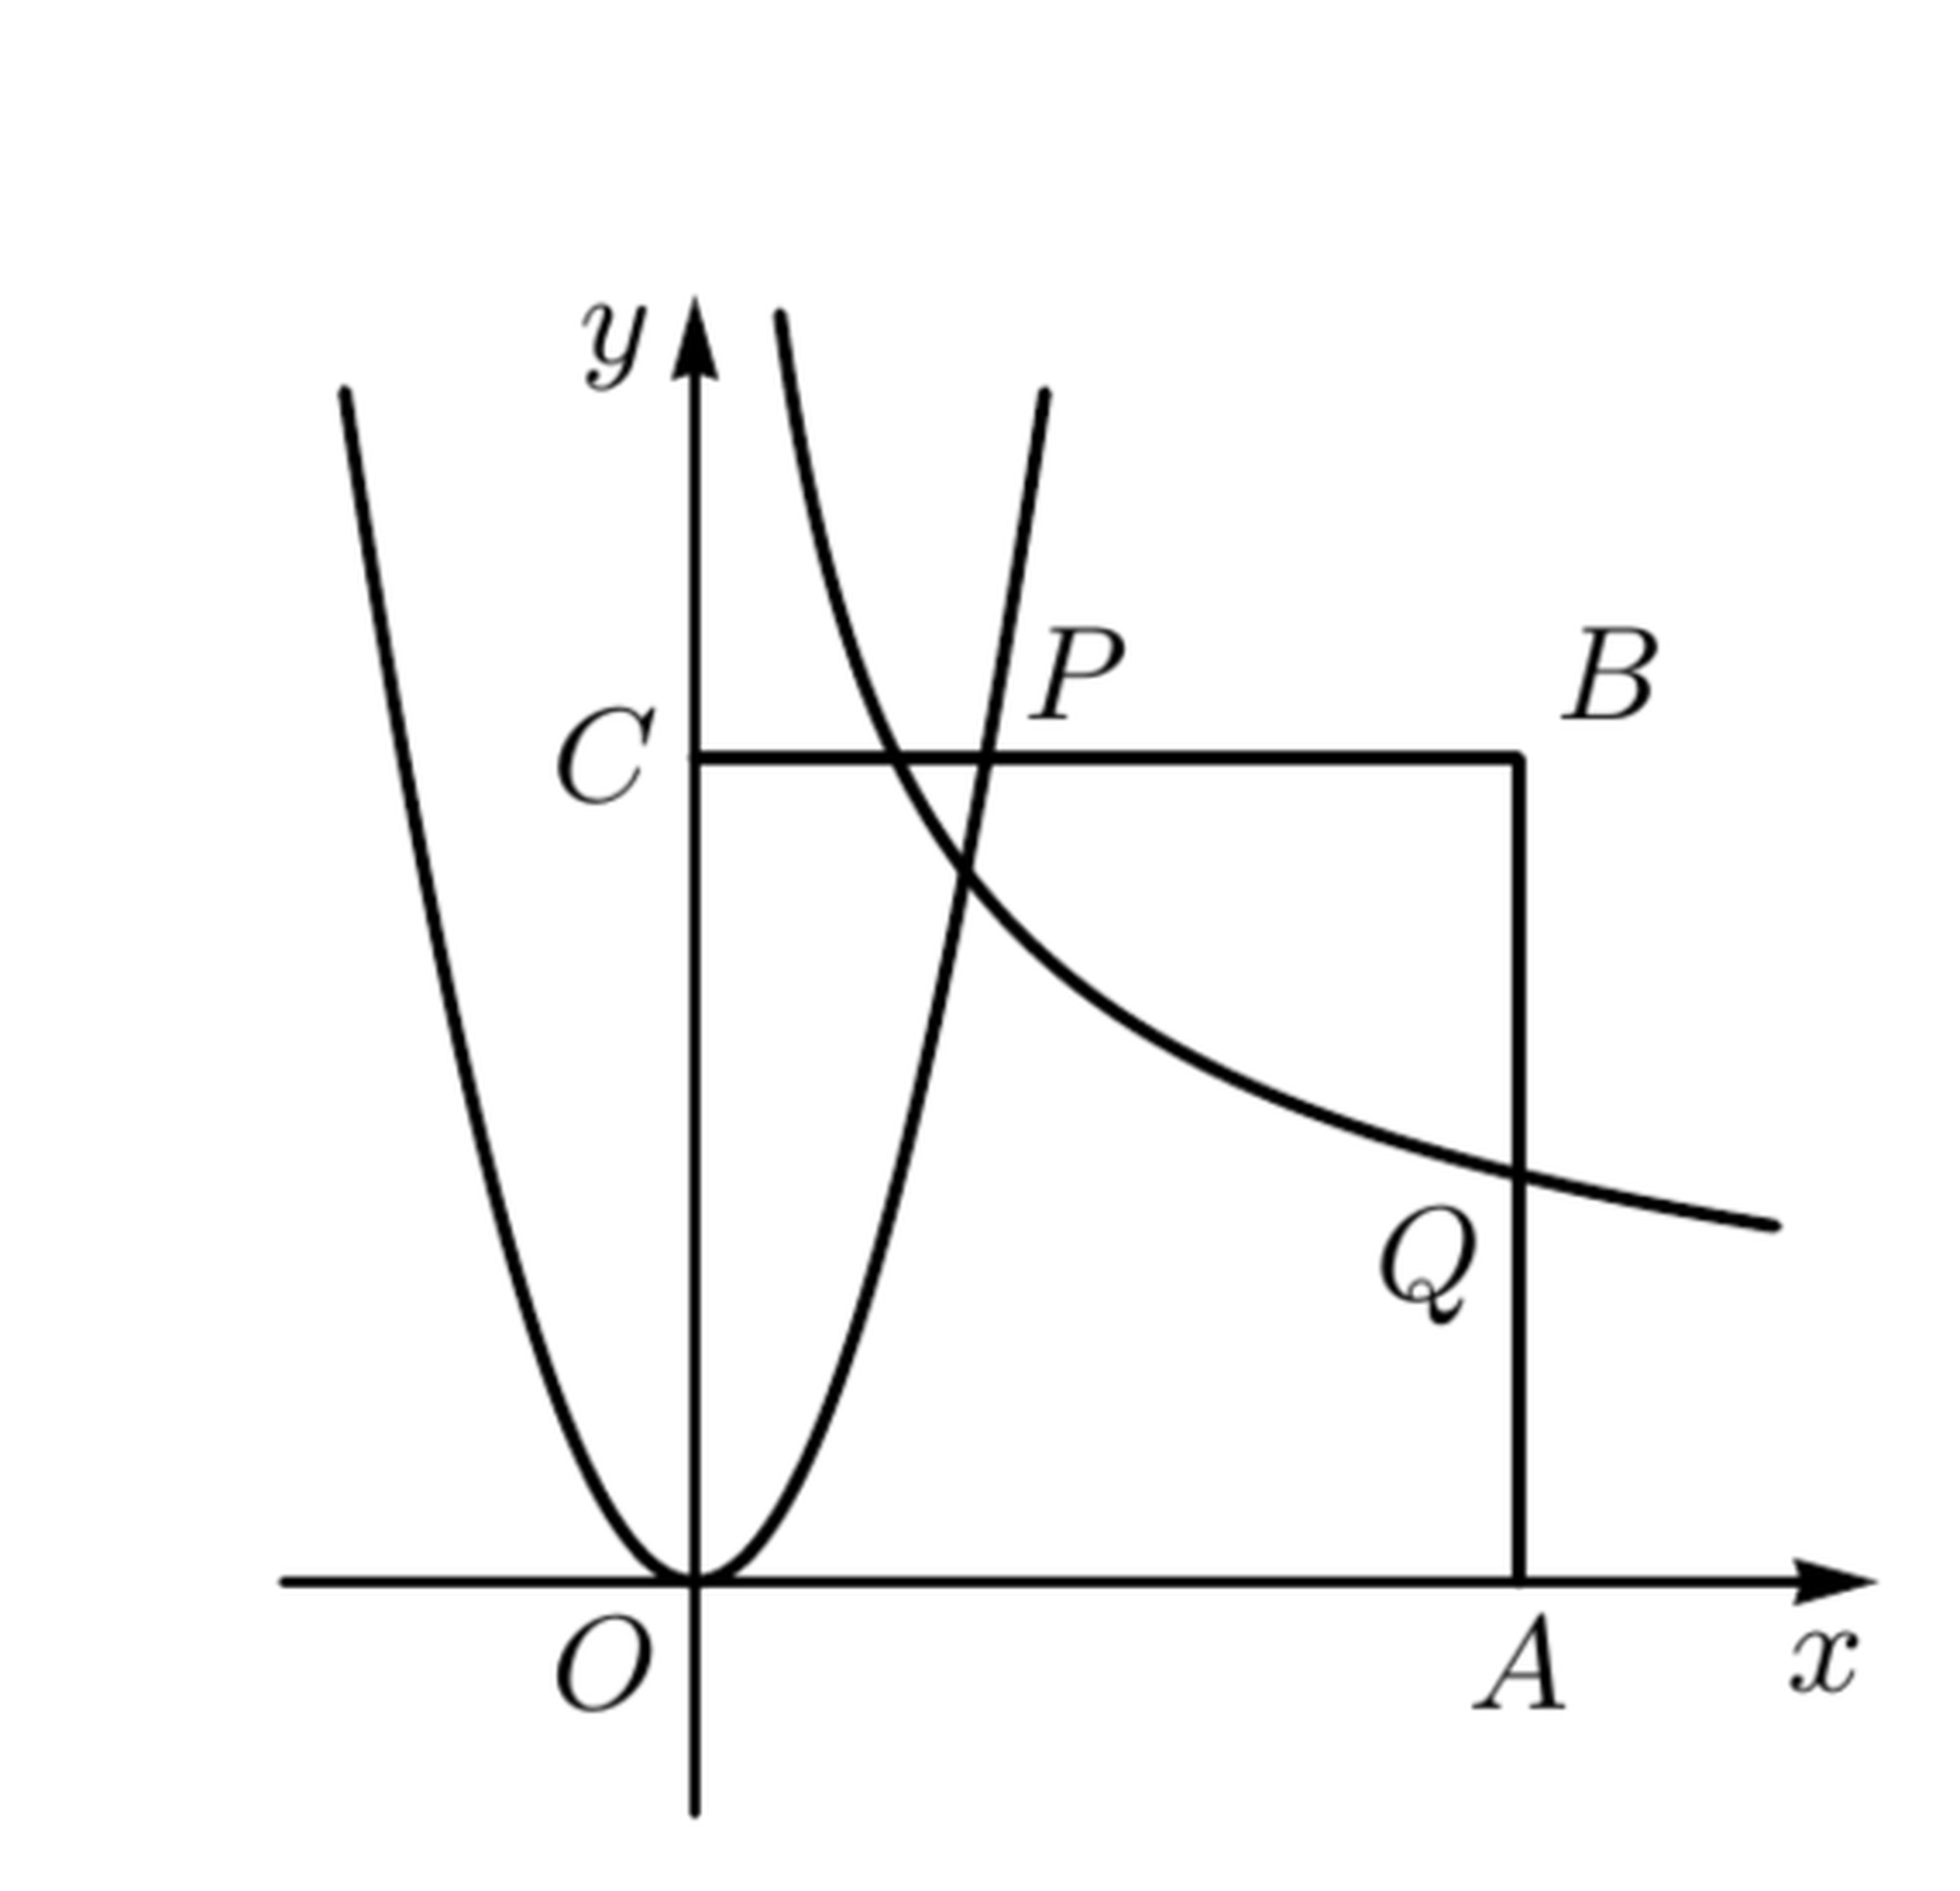
\includegraphics[width=0.40\textwidth]{figures/gao153_q11.png}
\end{center}

\ifanswer
\solbegin
\step{$\lvert AQ\rvert=\dfrac1{\sqrt a}$，$\lvert CP\rvert=\sqrt{\dfrac a5}$，}
\step{于是 $\lvert AQ\rvert+\lvert CP\rvert=\dfrac1{\sqrt a}+\sqrt{\dfrac a5}\geqslant2\sqrt{\dfrac1{\sqrt a}\cdot\sqrt{\dfrac a5}}=\dfrac2{\sqrt[4]{5}}$，}
\step{当且仅当 $\dfrac1{\sqrt a}=\sqrt{\dfrac a5}$，即 $a=\sqrt5$ 时取等号.}
\solend
\fi

% === Q12 === $B\subseteq A$ 带下划线照录、空集 \varnothing；解析 5 行
\item 若集合 $A=\{x\mid1\leqslant x\leqslant100,x\in\Z\}$，集合 $B\subseteq A$，且 $B\ne\varnothing$，记 $W(B)$ 为 $B$ 中元素的最大值与最小值之和，则对所有的 $B$，$W(B)$ 的平均值是\blankline[4.4em].

\ifanswer
\solbegin
\step{对每个非空子集 $B$，令 $B'=\{101-x\mid x\in B\}$，}
\step{则 $W(B')=(101-\min B)+(101-\max B)=202-W(B)$.}
\step{对 $B'$ 再作同样变换即得到 $B$，因此 $B$ 遍历所有非空子集时，}
\step{$B'$ 也恰好遍历所有非空子集.}
\step{设所求平均值为 $m$，则 $m=202-m$，解得 $m=101$.}
\solend
\fi

\end{enumerate}

\bigsec{二、选择题}

\begin{enumerate}
\setcounter{enumi}{12}

% === Q13 === "图像"（像，有亻）照录；解析 2 行，故选 A
\item 设 $a$、$b$ 为常数，若 $0<a<1$，$b>1$，则函数 $y=a^x-b$ 的图像必定不经过\mbox{（\quad）}

\keepwithprev
A. 第一象限\qquad\qquad B. 第二象限\qquad\qquad C. 第三象限\qquad\qquad D. 第四象限

\ifanswer
\solbegin
\step{当 $x>0$ 时，$a^x<1<b$，所以 $y=a^x-b<0$，图像必定不经过第一象限，}
\step{故选 $A$.}
\solend
\fi

% === Q14 === $m\in\Z$、中文弯引号、"图像"照录；解析 3 行，故选 A
\item 已知 $m\in\Z$，则“$m=0$”是“幂函数 $y=x^{m^2-2m-1}$ 的图像与 $x$ 轴及 $y$ 轴均无交点，且关于原点成中心对称”的\mbox{（\quad）}

\keepwithprev
A. 充分不必要条件\qquad\qquad B. 必要不充分条件

C. 充要条件\qquad\qquad D. 既不充分也不必要条件

\ifanswer
\solbegin
\step{图像满足所述条件 $\Leftrightarrow m^2-2m-1$ 为负奇数 $\Leftrightarrow m=0$ 或 $m=2$.}
\step{$m=0$ 能推出所述条件，但所述条件不能推出 $m=0$，因此是充分不必要条件，}
\step{故选 $A$.}
\solend
\fi

% === Q15 === 四选项一行；解析 5 行（跨 03→04 页），故选 D
\item 设 $a>b>1$，$x>1$，则下列不等式正确的是\mbox{（\quad）}

\keepwithprev
A. $a^x<b^x$\qquad B. $x^a<x^b$\qquad C. $\log_a x>\log_b x$\qquad D. $\log_x a>\log_x b$

\ifanswer
\solbegin
\step{$x>1$，幂函数与指数函数的单调性给出 $a^x>b^x$，$x^a>x^b$，A、B 错误.}
\step{$\log_a x=\dfrac{\lg x}{\lg a}<\dfrac{\lg x}{\lg b}=\log_b x$，C 错误.}
\step{对数函数 $y=\log_x t$ 的底数 $x>1$，在 $(0,+\infty)$ 上严格递增，}
\step{所以 $\log_x a>\log_x b$，D 正确.}
\step{故选 $D$.}
\solend
\fi

% === Q16 === $a\in\N$；解析 3 行，故选 C
\item 设 $a\in\N$，则满足不等式 $x^2-a^2x-a^2-1<0$ 的整数 $x$ 的个数不可能是\mbox{（\quad）}

\keepwithprev
A. 1\qquad\qquad B. 50\qquad\qquad C. 100\qquad\qquad D. 2026

\ifanswer
\solbegin
\step{$(x+1)(x-a^2-1)<0\Leftrightarrow-1<x<a^2+1$. 整数解为 $0,1,\cdots,a^2$，共 $a^2+1$ 个.}
\step{$1=0^2+1$，$50=7^2+1$，$2026=45^2+1$，而 $100-1=99$ 不是完全平方数，}
\step{故选 $C$.}
\solend
\fi

\end{enumerate}

\bigsec{三、解答题}

\begin{enumerate}
\setcounter{enumi}{16}

% === Q17 === 补集上划线 \overline{A}、\subseteq 照录；解析 5 行
\item 已知全集 $U=\R$，集合 $A=\{x\mid x^2-x-2\geqslant0\}$，$B=\{x\mid x>-1\}$，$C=\{x\mid a-5<x<a\}$.

(1) 求 $A\cap B$、$A\cup B$；

(2) 若 $\overline{A}\cup C=C$，求实数 $a$ 的取值范围.

\ifanswer
\solbegin
\step{(1) $x^2-x-2=(x+1)(x-2)\geqslant0\Leftrightarrow x\leqslant-1$ 或 $x\geqslant2$，}
\step{所以 $A=(-\infty,-1]\cup[2,+\infty)$，$B=(-1,+\infty)$，}
\step{因此 $A\cap B=[2,+\infty)$，$A\cup B=\R$.}
\step{(2) $\overline{A}=(-1,2)$，于是 $\overline{A}\cup C=C\Leftrightarrow\overline{A}\subseteq C\Leftrightarrow(-1,2)\subseteq(a-5,a)$，}
\step{两区间均为开区间，端点可重合，故 $\begin{cases}a-5\leqslant-1\\a\geqslant2\end{cases}\Leftrightarrow2\leqslant a\leqslant4$.}
\solend
\fi

% === Q18 === 解析 4 行
\item 已知 $a$、$b$、$c$ 都是正数，

(1) 若 $a+b=1$，求证：$\dfrac1a+\dfrac1b\geqslant4$，并指出等号成立的条件；

(2) 若 $a+b+c=1$，求证：三个数 $\dfrac1a$、$\dfrac1b$、$\dfrac1c$ 中至少有一个不小于 3.

\ifanswer
\solbegin
\step{(1) 由 $(a-b)^2\geqslant0$，得 $4ab\leqslant(a+b)^2=1$，所以 $\dfrac1a+\dfrac1b=\dfrac{a+b}{ab}=\dfrac1{ab}\geqslant4$，}
\step{等号成立当且仅当 $a=b$，结合 $a+b=1$，得 $a=b=\dfrac12$.}
\step{(2) 假设三个数 $\dfrac1a$、$\dfrac1b$、$\dfrac1c$ 都小于 3，则 $a>\dfrac13,b>\dfrac13,c>\dfrac13\Rightarrow a+b+c>1$，}
\step{与 $a+b+c=1$ 矛盾，因此三个数中至少有一个不小于 3.}
\solend
\fi

% === Q19 === 题目配图（三版都出）；\needvspace 守卫放 \item 之前；解析 19 行
\needvspace{8cm}
\item 某新建居民小区有一直角三角形绿地，两直角边长分别为 30m 和 40m，打算在其中划出一片区域改造成活动场地，如图所示.

(1) 若划出的区域为正方形，且有两边落在绿地边界上，求此正方形边长；

(2) 若划出的区域为圆形，求圆形区域面积的最大值；

(3) 若划出的区域为矩形（其中至少有一边在边界上），求此矩形面积的最大值.

\begin{center}
% 直角三角形 ABC 绿地示意图取 05 页右上，去粉色水印、去色、4× LANCZOS 放大；三版都出
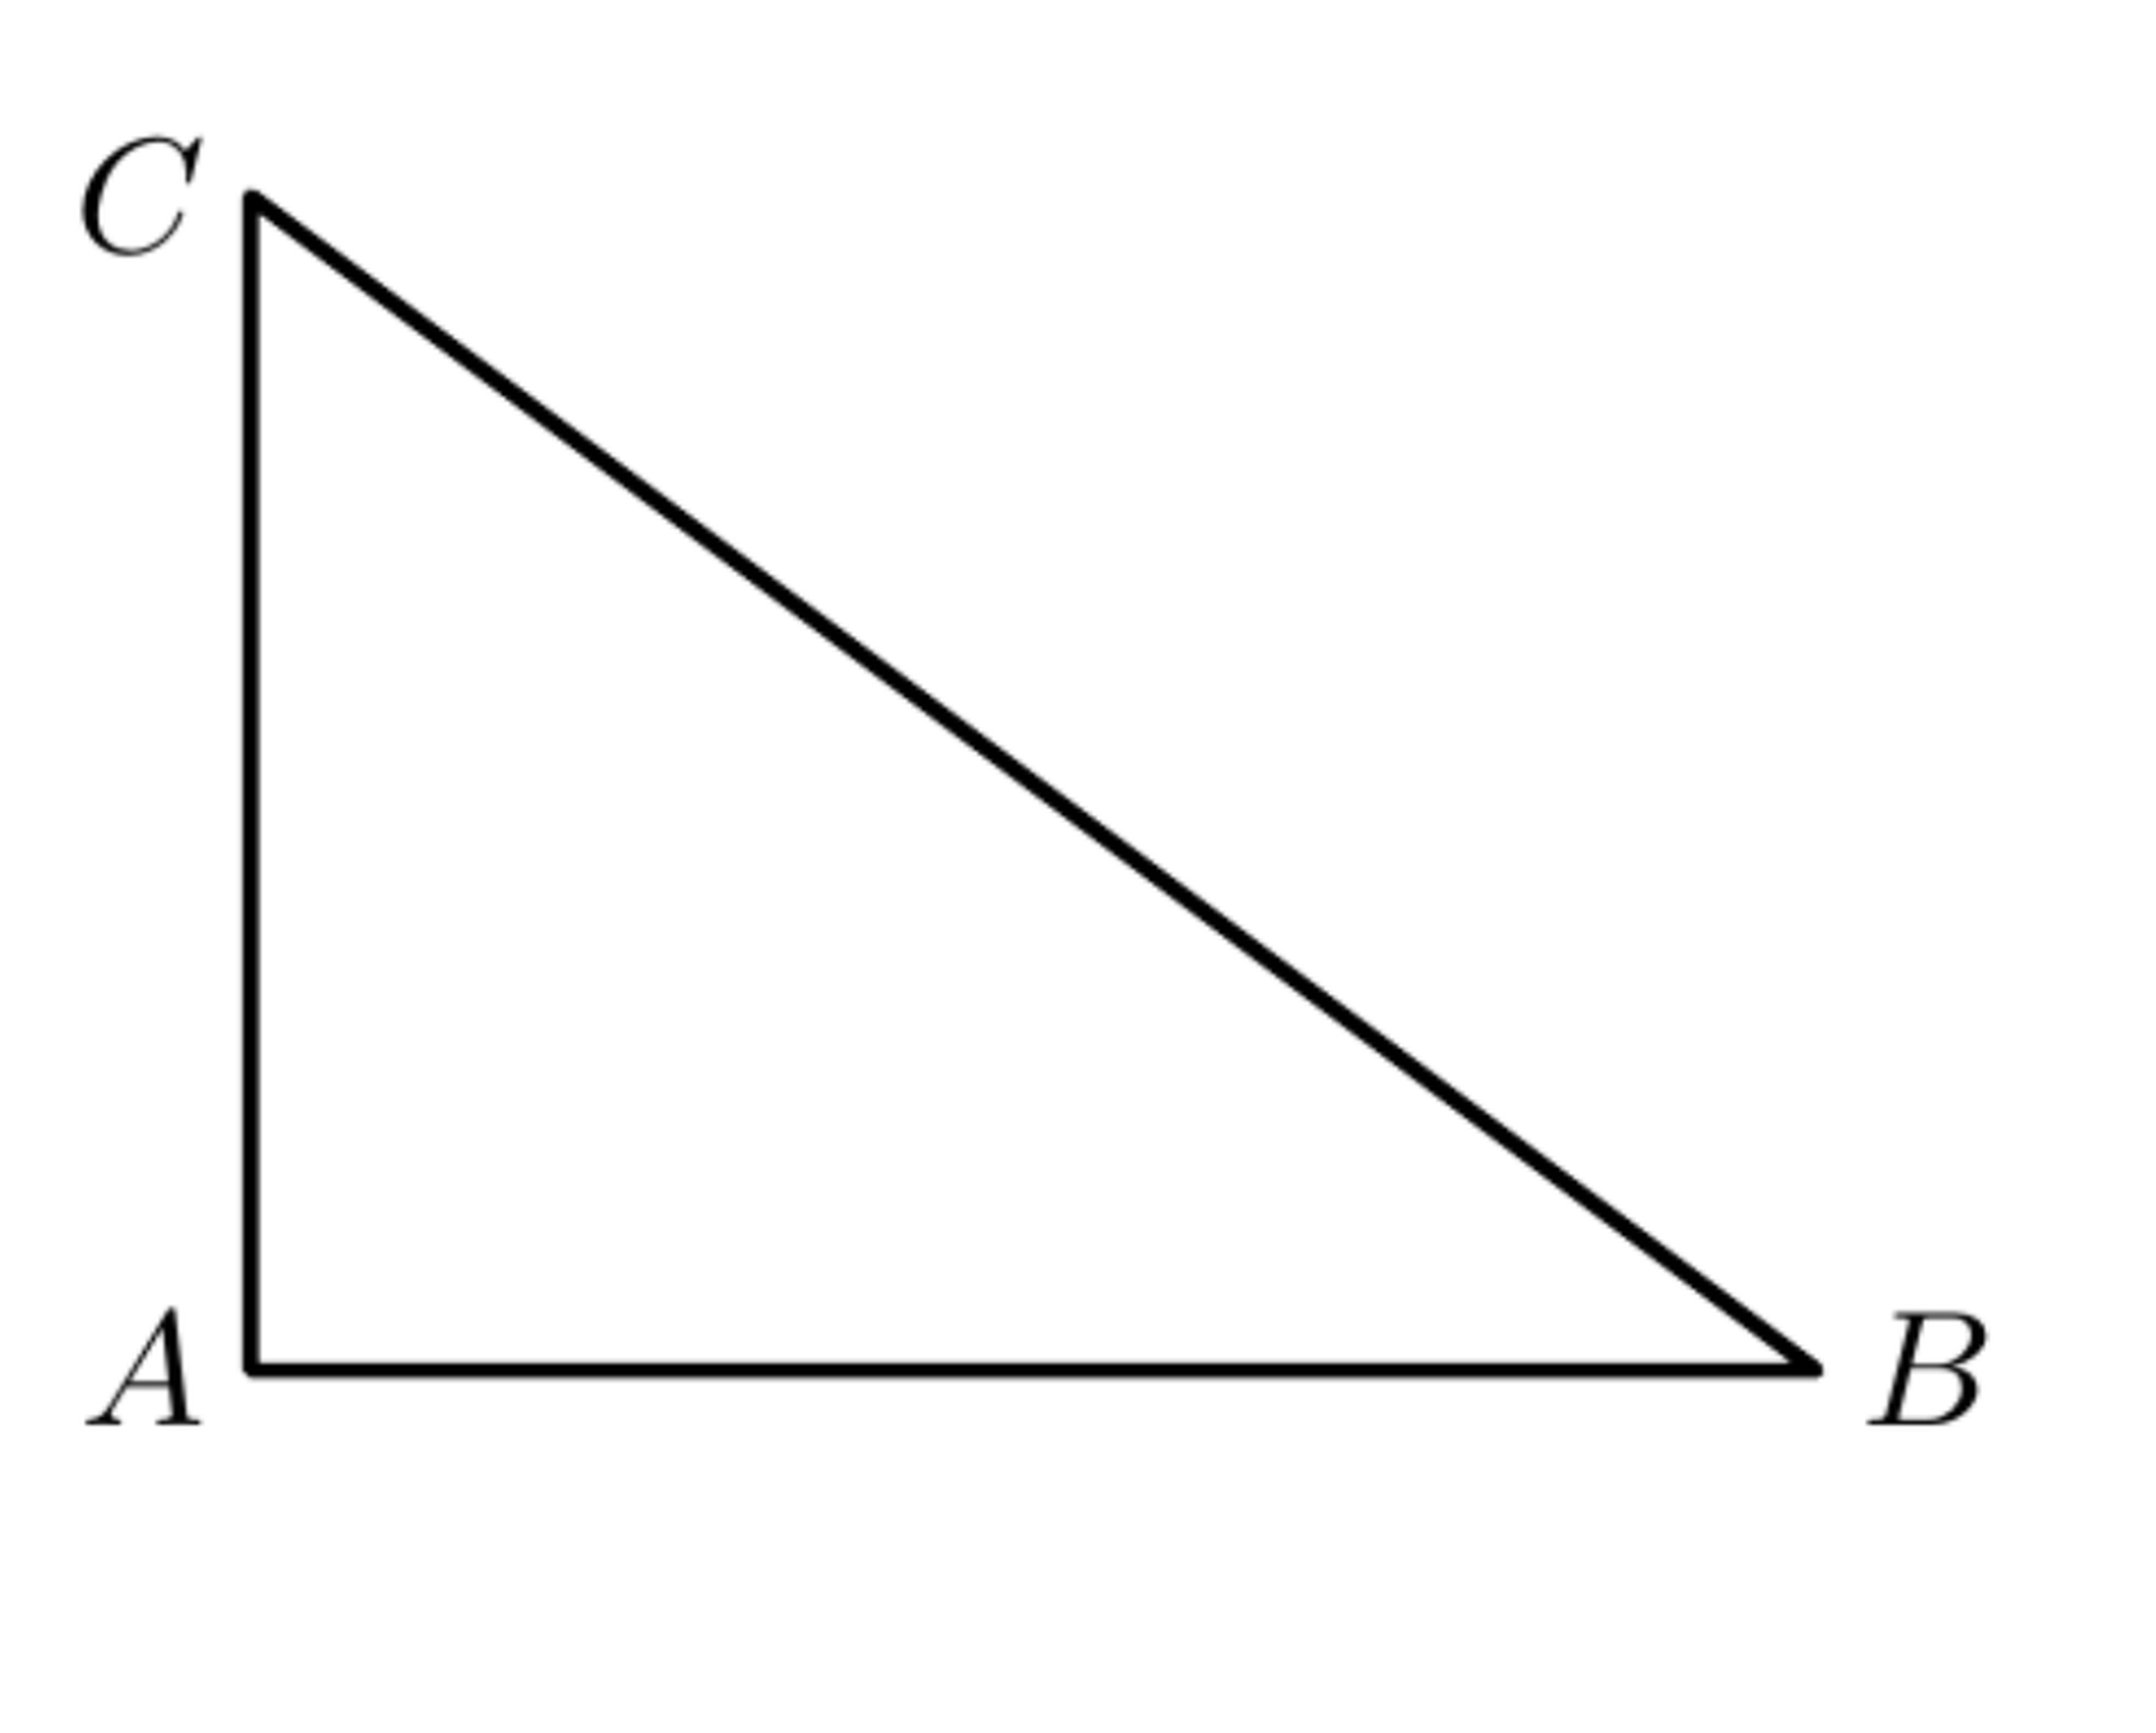
\includegraphics[width=0.34\textwidth]{figures/gao153_q19.png}
\end{center}

\ifanswer
\solbegin
\step{(1) 取 $A(0,0)$、$B(40,0)$、$C(0,30)$，则斜边 $BC$ 所在直线为 $3x+4y=120$.}
\step{正方形落在边界上的两边必分别在两条直角边上.}
\step{设其边长为 $a$m，则对角顶点为 $(a,a)$.}
\step{按题意划出的正方形应尽量大，即对角顶点落在斜边 $BC$ 上，}
\step{因此 $3a+4a=120\Rightarrow a=\dfrac{120}{7}$；}
\step{(2) 斜边长 $BC=\sqrt{30^2+40^2}=50$m，三角形面积为 $600\text{m}^2$.}
\step{设圆的半径为 $r$，圆心到 $AB$、$AC$、$BC$ 的距离分别为 $d_1,d_2,d_3$，}
\step{则三者均不小于 $r$. 连接圆心与三个顶点，}
\step{得 $600=\dfrac12(40d_1+30d_2+50d_3)\geqslant\dfrac12(40+30+50)r=60r$，所以 $r\leqslant10$.}
\step{取三角形的内切圆时等号成立，圆形区域面积的最大值为 $100\pi\text{m}^2$.}
\step{(3) 任取矩形落在绿地边界上的一边，以其所在直线为横轴.}
\step{设相应三角形底边长为 $L$、高为 $H$，则 $LH=1200$.}
\step{取三角形顶点坐标为 $(0,0)$、$(L,0)$、$(p,H)$.}
\step{在高度 $t$ 处，两腰上的点的横坐标分别为 $\dfrac{pt}{H}$、$L+\dfrac{(p-L)t}{H}$，}
\step{因此，高为 $t$ 的矩形，其底边长不超过 $L\left(1-\dfrac tH\right)$，}
\step{面积满足 $S\leqslant Lt\left(1-\dfrac tH\right)=\dfrac LH\left[\dfrac{H^2}{4}-\left(t-\dfrac H2\right)^2\right]\leqslant\dfrac{LH}{4}=300$，}
\step{在原坐标系中，取矩形顶点为 $(0,0)$、$(20,0)$、$(20,15)$、$(0,15)$，}
\step{其中 $3\times20+4\times15=120$，矩形完全位于绿地内，面积为 $300\text{m}^2$，}
\step{达到最大值.}
\solend
\fi

% === Q20 === $g(x)$ 定义照录；解析 14 行
\item 已知 $a>0$ 且 $a\ne1$，设 $f(x)=\log_a(x^2-a^2)$，$g(x)=2\log_a(x-ak)$.

(1) 求函数 $y=f(x)$ 的定义域；

(2) 若 $k=2$，求不等式 $f(x)>g(x)$ 的解集；

(3) 若“存在实数 $x$，使得 $f(x)=g(x)$”为真命题，求实数 $k$ 的取值范围.

\ifanswer
\solbegin
\step{(1) $x^2-a^2>0\Leftrightarrow x<-a$ 或 $x>a$，定义域为 $(-\infty,-a)\cup(a,+\infty)$.}
\step{(2) 两函数均有意义时，$x>2a$，且 $g(x)=\log_a(x-2a)^2$.}
\step{当 $a>1$ 时，$f(x)>g(x)\Leftrightarrow x^2-a^2>(x-2a)^2\Leftrightarrow x>\dfrac{5a}{4}$，}
\step{结合 $x>2a$，解集为 $(2a,+\infty)$.}
\step{当 $0<a<1$ 时，$f(x)>g(x)\Leftrightarrow x^2-a^2<(x-2a)^2\Leftrightarrow x<\dfrac{5a}{4}$，}
\step{与 $x>2a$ 矛盾，解集为 $\varnothing$.}
\step{(3) 在 $x^2-a^2>0$ 且 $x-ak>0$ 的条件下，}
\step{$f(x)=g(x)\Leftrightarrow x^2-a^2=(x-ak)^2\Leftrightarrow2akx=a^2(1+k^2)$，}
\step{当 $k=0$ 时，上式不成立；}
\step{当 $k\ne0$ 时，$x=\dfrac{a(1+k^2)}{2k}$，}
\step{于是 $x-ak=\dfrac{a(1-k^2)}{2k}>0\Leftrightarrow k<-1$ 或 $0<k<1$，}
\step{对上述 $k$，所取的 $x$ 同时满足 $x^2-a^2=(x-ak)^2>0$，}
\step{两函数均有意义且函数值相等.}
\step{因此，$k$ 的取值范围为 $(-\infty,-1)\cup(0,1)$.}
\solend
\fi

% === Q21 === 中文弯引号、复杂式照录；解析 23 行（跨 08→09 页）
\item 若实数 $x$、$y$、$m$ 满足 $\lvert x-m\rvert<\lvert y-m\rvert$，则称 $x$ 比 $y$ 接近 $m$.

(1) 若 $2x$ 比 $x-2$ 更接近 1，求实数 $x$ 的取值范围；

(2) 若 $x$ 比 $y$ 接近 $m$，证明：“$x>y$” 的充要条件是 “$x+y<2m$”；

(3) 已知 $x>0$，$y>0$ 且 $x\ne y$. 设 $p=\dfrac{x^2+y^2}{xy}$，若对于任意的 $x$、$y$，命题 “$p$ 比 $p^2-3p+4$ 接近 $m$” 恒成立，求实数 $m$ 的取值范围.

\ifanswer
\solbegin
\step{(1) $\lvert2x-1\rvert<\lvert x-3\rvert\Leftrightarrow(2x-1)^2<(x-3)^2\Leftrightarrow(x+2)(3x-4)<0$，}
\step{解得 $-2<x<\dfrac43$，实数 $x$ 的取值范围为 $\left(-2,\dfrac43\right)$.}
\step{(2) 因为 $x$ 比 $y$ 接近 $m$，所以 $\lvert x-m\rvert<\lvert y-m\rvert$，则 $\lvert x-m\rvert^2<\lvert y-m\rvert^2$，}
\step{即 $(x-m)^2<(y-m)^2$，即 $(x-m)^2-(y-m)^2<0$，}
\step{即得 $(x-y)(x+y-2m)<0$，}
\step{则由 $x+y<2m$，得 $x+y-2m<0$，}
\step{故 $x-y>0$，即 $x>y$，充分性成立；}
\step{当 $x>y$ 时，$x-y>0$，结合 $(x-y)(x+y-2m)<0$，得 $x+y-2m<0$，}
\step{即 $x+y<2m$，必要性成立；}
\step{故“$x>y$” 的充要条件是 “$x+y<2m$”；}
\step{(3) $x>0$，$y>0$ 且 $x\ne y$. 则 $p=\dfrac{x^2+y^2}{xy}=\dfrac xy+\dfrac yx>2\sqrt{\dfrac xy\cdot\dfrac yx}=2$，}
\step{由于对于任意的 $x$、$y$，命题 “$p$ 比 $p^2-3p+4$ 接近 $m$” 恒成立，}
\step{故 $\lvert p-m\rvert<\lvert(p^2-3p+4)-m\rvert$ 对 $\forall p>2$ 恒成立，}
\step{即得 $(p-m)^2<(p^2-3p+4-m)^2$，}
\step{即 $(p^2-3p+4-m)^2-(p-m)^2>0$，}
\step{得 $(p^2-4p+4)(p^2-2p+4-2m)>0$，}
\step{即 $(p-2)^2(p^2-2p+4-2m)>0$，由于 $p>2$，故 $(p-2)^2>0$，}
\step{故 $p^2-2p+4-2m>0$ 对 $\forall p>2$ 恒成立，}
\step{即 $2m<p^2-2p+4$ 对 $\forall p>2$ 恒成立，}
\step{由于 $p^2-2p+4=(p-1)^2+3$，此时 $p^2-2p+4$ 在 $(2,+\infty)$ 上严格增，}
\step{故 $(p-1)^2+3>(2-1)^2+3=4$，故 $2m\leqslant4$，解得 $m\leqslant2$，}
\step{即实数 $m$ 的取值范围是 $(-\infty,2]$.}
\solend
\fi

\end{enumerate}

\end{document}
"
% 紧凑版：xelatex "\def\iscompact{1}% 高一153_闵行中学文绮中学_期中.tex
%   —— 高一上数学"2026-2027 年闵行中学文绮中学高一上期中"（试卷版/答案版/紧凑版）
% 试卷版：xelatex 高一153_闵行中学文绮中学_期中.tex
% 答案版：xelatex "\def\isanswer{1}% 高一153_闵行中学文绮中学_期中.tex
%   —— 高一上数学"2026-2027 年闵行中学文绮中学高一上期中"（试卷版/答案版/紧凑版）
% 试卷版：xelatex 高一153_闵行中学文绮中学_期中.tex
% 答案版：xelatex "\def\isanswer{1}\input{高一153_闵行中学文绮中学_期中.tex}"
% 紧凑版：xelatex "\def\iscompact{1}\input{高一153_闵行中学文绮中学_期中.tex}"
%
% ① 原始材料：微信公众号"魔都数学加油站"文章，连载"27学年高一153"，原文标题
% "27学年高一153——2026-2027年上海市闵行中学文绮中学高一上期中"；
% 原文链接：https://mp.weixin.qq.com/s/rEtS-92cDR6JKgY2b5DRfg 。
% 正文为 9 张 PNG 页（01/02/06/07/08/09 为 2560×3620，03/04/05 为 4762×6735，
% 同一篇各页分辨率混排，逐页按各自分辨率裁图核对，别按预览比例换算裁框）。
% 体例：讲评版——填空 3—12（10 题）、选择 13—16（4 题）、解答 17—21（5 题），
% 共 19 题，自第 3 题起编；**全 19 题均印【解析】**（逐题核实，见 ② ②）。
% 题目、答案、解析均据原图转录；卷面粉红色水印"魔都数学加油站"及公众号页脚未录入。
% 全卷插图清单（逐页通读 9 页确认）：2 幅，均为题目配图、三版都出——
%   · Q11 正方形 OABC 曲线图（02 页右下：$y=5x^2$ 与 $y=x^{-\frac12}$ 两条曲线、
%     坐标轴、O/A/B/C/P/Q、正方形），裁 figures/gao153_q11.png；
%   · Q19 直角三角形 ABC 绿地示意图（05 页右上，直角在 A），
%     裁 figures/gao153_q19.png；
%   两图均去粉色水印、去色、4× LANCZOS 放大；Q11 图左上角题干残字"函"已裁白。
%   其余各页逐页确认无其它题目配图、无解析内配图、无表格；09 页下半仅水印、无正文。
%
% 卷首标题：原卷印作"2026-2027 年闵行中学文绮中学高一上期中"，年份区间按全稿惯例排 en dash；
% 原卷卷面未印副标题，本稿按同期中卷知识模块口径补出"集合与常用逻辑用语、不等式、函数"。
%
% ② 与原卷的排版差异：
%   ① 原文从第 3 题起，本稿保留原题号；共 19 题三节，解答题 5 题到 21；
%   ② 全 19 题均印【解析】、用 \solbegin…\solend，无只印【答案】或答案印括号内的题；
%      四道选择题答案在解析末句"故选 A／A／D／C"（Q13—Q16，逐个放大复核）、
%      括号 \mbox{（\quad）} 留空、不另提 \ans{}；答案版【答案】/【解析】标记数
%      = 19 = 全卷题数；
%   ③ 原卷卷面未印副标题，本稿按知识模块口径补出；
%   ④ 原卷填空横线按全稿惯例排 \blankline[4.4em]；选择题括号排 \mbox{（\quad）}、
%      四道选择题的选项段前按惯例各加 \keepwithprev；解答题不留作答区、不加
%      \anspace（原卷为讲评版，109—113 起全稿不用 \anspace）；
%   ⑤ 数集：Q3"$x\in R$"、Q5"解集为 R"、Q10"$x\in N$"、Q12"$x\in Z$"与
%      "$m\in Z$"、Q14"$m\in Z$"、Q16"$a\in N$"、Q17"全集 $U=R$"、
%      Q19 无、Q21 无——原卷印斜体或正体粗体 R/N/Z，按全稿惯例归一
%      \R／\N／\Z；绝对值排 \lvert…\rvert（Q5、Q11、Q21），集合描述竖线排 \mid
%      （Q3、Q10、Q17、Q20），不等号按全稿惯例排 \leqslant／\geqslant；
%      补集照原卷上划线排 \overline{A}（Q17 题干 (2)＋解析 (2)）；
%      空集 \varnothing（Q12 题干、Q20 解析 (2)）；子集 3 处均印带下划线 ⊆、
%      照录 \subseteq（Q10 $A\subseteq U$、Q12 $B\subseteq A$、Q17 $(-1,2)\subseteq(a-5,a)$），
%      本卷无单线 \subset 用例；
%   ⑥ 判别式：逐页通读 9 页，本卷无一元二次判别式 Δ/△ 算式，故无 Δ/△ 混用可照录；
%      Q11 图里有几何正方形 OABC（非三角形符号），无 △ABC 用例；
%   ⑦ 中文弯引号照录：Q14"$m=0$"与"幂函数…关于原点成中心对称"、
%      Q20"存在实数 $x$，使得 $f(x)=g(x)$"、Q21"$x>y$"与"$x+y<2m$"、
%      "$p$ 比 $p^2-3p+4$ 接近 $m$"（引号外留空格按原卷）；
%      注释里一律 ASCII 引号；数学式内 CJK 用 \text{}；
%   ⑧ "图像／图象"逐处放大核：全卷 3 处均印"图像"（像，有亻）——
%      Q13 题干与解析、Q14 题干与解析；Q19 题干写"如图所示"（非"图像"），
%      逐处照录未统一；子题标号 (1)(2)(3) 半角括号照录；圈数字本卷无用例；
%   ⑨ 半角逗号在数学组之间是全稿惯例、非笔误，逐处照录（Q3 $x\in R$、
%      Q10 $a_1,a_2$、Q19 $A(0,0)$、$d_1,d_2,d_3$、Q21 $a>\frac13,b>\frac13$ 等）；
%      行末西文句点 ASCII `.`；行中全角逗号／顿号照录（Q19"30m 和 40m"、
%      Q21"实数 $x$、$y$、$m$"）；
%   ⑩ 复杂式照录别简化：Q3 $y=x^{-2}$、Q11 $y=x^{-\frac12}$ 与
%      $\frac{2}{\sqrt[4]{5}}$、Q8 $\frac{2b}{a+1-b}$、Q9 cases 块、
%      Q10 $525=5\times105$、Q16 $a^2+1$、Q19 $S\leqslant Lt(1-\frac tH)$
%      与 $L+\frac{(p-L)t}{H}$、Q20 $2akx=a^2(1+k^2)$ 与 $\frac{a(1+k^2)}{2k}$、
%      Q21 $(p^2-4p+4)(p^2-2p+4-2m)>0$；
%      \left…\right 不得拆到不同 $…$ 组（Q17 $\left\{x\mid\cdots\right\}$、
%      Q19 $\left[\frac{H^2}{4}-\left(t-\frac H2\right)^2\right]$、
%      Q21 $\left(-2,\frac43\right)$ 等）；cases 块一律 \begin{cases}…\end{cases}；
%   ⑪ 一条 \step = 原卷解析的一个印刷行，cases 块整体算一个印刷行；别并折行、
%      别拆行。Q10 六行、Q19 十九行、Q20 十四行、Q21 二十二行均按印刷行逐条断，
%      不丢行；
%   ⑫ 配图：Q11／Q19 题目配图（三版都出）放 \item 内题干之后 \begin{center}，
%      各用 \needvspace{8cm} 守卫把整块推走，**守卫放在 \item 之前**
%      （见 高一145 Q14/Q20 成例与切页审计 B 类坑）；
%   ⑬ 原卷解析内无红色"法一／法二"之类小标题，故本卷无 \stepm；红色水印
%      "魔都数学加油站"不录入；
%   ⑭ 跨页续印按题合并：见 ⑥；
%
% ③ 行数复核：一条 \step = 原卷解析的一个印刷行，cases 块作一个印刷行计。
%   逐题数（主会话逐页核对定稿）：Q3：1；Q4：2；Q5：2；Q6：2；Q7：1；
%   Q8：1；Q9：2；Q10：6；Q11：3；Q12：5；Q13：2；Q14：3；Q15：5；
%   Q16：3；Q17：5；Q18：4；Q19：19；Q20：14；Q21：22。
%   合计 102 条 \step（本卷无 \stepm），与原卷逐题印刷行相等。全卷 19 题
%   均设 \solbegin…\solend，答案版【答案】/【解析】标记数 = 19 = 全卷题数。
%
% ④ 判别式／子集符号结论（逐处放大原图照录、不得统一，主会话像素级复核）：
%   判别式：逐页通读 9 页，本卷无一元二次判别式算式（Q7 用韦达定理、
%      Q16 用因式分解、Q20 用对数方程，均不写 Δ/△），故无 Δ/△ 混用可照录
%      （"高 \Delta／扁 \triangle"口径备查，参照 高一142／151／152 头注）；
%      本卷无几何三角形符号用例。
%   子集：Q10 题干"$A\subseteq U$"、Q12 题干"$B\subseteq A$"、Q17 解析 (2)
%      "$(-1,2)\subseteq(a-5,a)$"共 3 处，逐处放大确认均印带下划线 ⊆、
%      照录 \subseteq；本卷未见单线 ⊂（\subset）之对应处。
%      补集上划线 \overline{A}（Q17）、空集 \varnothing（Q12 题干、Q20 解析 (2)）；
%      数集 \R／\N／\Z 归一见 ② ⑤。
%
% ⑤ 存疑照录（放大原图确认，照录未改、正文对应处另有 % 注）：
%   1. Q3 集合 $B=\{(x,y)\mid y=x^{-2},x\in\R\}$ 原卷题干径写 $x\in\R$
%      （$x=0$ 处无意义），解析自行注明 $x\ne0$，照录未改。
%   2. Q10 解析"$U$ 中共有 $525=5\times105$ 个连续整数"与尾行
%      "取 $U$ 中除以 5 余 1 或 2 的全部元素及元素 5"逐字照录（放大 02 页
%      /tmp/gao153/z/zoom/q10_pick.png 确认是"元素 5"，非"元素 9"）。
%   3. Q11 第二个函数原卷印 $y=x^{-\frac12}$（负二分之一次幂，非 $x^2$），
%      放大 02 页 /tmp/gao153/z/zoom/q11_exp.png 确认，照录未改；
%      $|AQ|=\frac1{\sqrt a}$ 与之自洽。
%   4. Q19 (3) 解析"在高度 $t$ 处，两腰上的点的横坐标分别为 $\frac{pt}{H}$、
%      $L+\frac{(p-L)t}{H}$"，放大 06 页确认，照录未简化。
%   5. Q20 (2) 解析"$g(x)=\log_a(x-2a)^2$"（真数整体平方），
%      与 $g(x)=2\log_a(x-ak)$ 在 $k=2$ 时一致，照录未改。
%   6. Q21 (3) 解析"得 $(p^2-4p+4)(p^2-2p+4-2m)>0$"与
%      "故 $(p-1)^2+3>(2-1)^2+3=4$，故 $2m\leqslant4$"照录未改
%      （放大 09 页 /tmp/gao153/z/zoom/q21_factor.png 确认）。
%   7. "图像／图象"全卷 3 处均印"图像"（像，有亻）逐处照录；
%      本卷无判别式 Δ/△ 用例（见 ④）。
%   全卷除此 7 类外未发现其它笔误／自相矛盾处；19 题均印【解析】、
%   无只印【答案】或答案印括号内的题（见 ② ②）。
%
% ⑥ 跨页续印按题合并说明（逐页核实定稿）：Q3—Q5 题干＋解析在 01 页；
%   Q6—Q8 题干＋解析在 01 页下半（Q8 解析续 02 页顶）；Q9 题干＋解析、
%   Q10 题干＋解析首 2 行在 02 页上半，Q10 解析余 4 行在 02 页下半；
%   Q11 题干＋配图＋解析、Q12 题干＋解析 5 行在 02 页下半—03 页上半；
%   "二、选择题"标题在 03 页中部；Q13 题干＋选项＋解析在 03 页下半；
%   Q14 题干＋选项＋解析、Q15 题干＋选项＋解析首行在 03 页下半—04 页顶；
%   Q15 解析余 4 行、Q16 题干＋选项＋解析在 04 页上半；"三、解答题"
%   标题在 04 页下半；Q17 题干＋两问＋解析 5 行在 04 页下半—05 页顶；
%   Q18 题干＋两问＋解析 4 行、Q19 题干（含配图）＋三问在 05 页；
%   Q19 解析 (1)(2) 9 行在 05 页下半，解析 (3) 前 5 行在 06 页上半、
%   余 4 行在 06 页下半；Q20 题干＋三问在 06 页下半，解析 (1)(2)(3)
%   前 6 行在 07 页上半、(3) 余 8 行在 07 页下半；Q21 题干＋三问在
%   07 页末，解析 (1)(2) 10 行在 08 页上半—下半，解析 (3) 前 4 行在
%   08 页下半、余 9 行续 09 页上半，末行"即实数 $m$ 的取值范围是
%   $(-\infty,2]$"为全卷收尾（09 页下半仅水印、无正文）。
%   本稿按题连排，不丢行、不并折行；全卷末题为第 21 题，无附加题节。
%
\documentclass[a4paper,11pt]{article}
\usepackage{common}

\begin{document}

\examtitlest[3]{2026--2027 年闵行中学文绮中学高一上期中}{集合与常用逻辑用语、不等式、函数}

\bigsec{一、填空题}

\begin{enumerate}
\setcounter{enumi}{2}

% === Q3 === 集合描述竖线 \mid；$y=x^{-2}$ 照录；解析 1 行
\item 已知 $A=\{(x,y)\mid y=x^3,x\in\R\}$，$B=\{(x,y)\mid y=x^{-2},x\in\R\}$，则 $A\cap B=$\blankline[4.4em].

\ifanswer
\solbegin
\step{$x^3=x^{-2}\ (x\ne0)\Leftrightarrow x^5=1\Leftrightarrow x=1$，此时 $y=1$，所以 $A\cap B=\{(1,1)\}$.}
\solend
\fi

% === Q4 === 解析 2 行
\item 若关于 $x$ 的不等式 $\dfrac{x-a}{x+1}>0$ 的解集为 $(-\infty,-1)\cup(4,+\infty)$，则实数 $a=$\blankline[4.4em].

\ifanswer
\solbegin
\step{关于 $x$ 的不等式 $\dfrac{x-a}{x+1}>0$ 即 $(x+1)(x-a)>0$.}
\step{再由它的解集为 $(-\infty,-1)\cup(4,+\infty)$，得 $-1$ 和 4 是 $(x+1)(x-a)=0$ 的两个实数根，故 $a=4$.}
\solend
\fi

% === Q5 === 绝对值 \lvert…\rvert；解析 2 行
\item 若关于 $x$ 的不等式 $\lvert x+1\rvert+\lvert x-2\rvert>m$ 的解集为 $\R$，则实数 $m$ 的取值范围是\blankline[4.4em].

\ifanswer
\solbegin
\step{$\lvert x+1\rvert+\lvert x-2\rvert\geqslant\lvert(x+1)-(x-2)\rvert=3$，当且仅当 $-1\leqslant x\leqslant2$ 时取等号，}
\step{因此 $m<3$.}
\solend
\fi

% === Q6 === 解析 2 行
\item 已知指数函数 $y=a^x$（$a>1$）在区间 $[-1,1]$ 上的最大值比最小值大 $\dfrac32$，则实数 $a=$\blankline[4.4em].

\ifanswer
\solbegin
\step{$a>1$，指数函数在 $[-1,1]$ 上严格增，故 $a-\dfrac1a=\dfrac32\Leftrightarrow(a-2)(2a+1)=0$.}
\step{结合 $a>1$，得 $a=2$.}
\solend
\fi

% === Q7 === 韦达定理；解析 1 行
\item 已知关于 $x$ 的一元二次方程 $x^2+px+2p=0$ 的两个实数根分别为 $x_1$、$x_2$，且 $(x_1+1)(x_2+1)=0$，则 $p=$\blankline[4.4em].

\ifanswer
\solbegin
\step{$0=(x_1+1)(x_2+1)=x_1x_2+x_1+x_2+1=2p-p+1=p+1\Rightarrow p=-1$.}
\solend
\fi

% === Q8 === 换底公式；解析 1 行
\item 已知 $10^a=3$，$\lg5=b$，则 $\log_6 25=$\blankline[4.4em]（用关于 $a,b$ 的关系式表示）.

\ifanswer
\solbegin
\step{$\lg3=a$，$\lg2=1-b$，所以 $\log_6 25=\dfrac{\lg25}{\lg6}=\dfrac{2b}{a+1-b}$.}
\solend
\fi

% === Q9 === cases 块整体算一个印刷行；解析 2 行
\item 已知 $A=[2,5]$，若对任意 $x\in A$，总有 $\dfrac{k}{x}\in A$，则正数 $k=$\blankline[4.4em].

\ifanswer
\solbegin
\step{$k>0$，当 $x\in[2,5]$ 时，$\dfrac{k}{x}$ 的取值范围为 $\left[\dfrac k5,\dfrac k2\right]$，}
\step{因此 $\begin{cases}\dfrac k5\geqslant2\\\dfrac k2\leqslant5\end{cases}\Leftrightarrow10\leqslant k\leqslant10\Leftrightarrow k=10$.}
\solend
\fi

% === Q10 === $A\subseteq U$ 带下划线照录；解析 6 行
\item 已知集合 $U=\{x\mid4\leqslant x\leqslant528,x\in\N\}$，$A=\{a_1,a_2,a_3,\cdots,a_n\}$，且 $A\subseteq U$. 如果集合 $A$ 中的任意两个不同元素之和都不能被 5 整除，则正整数 $n$ 的最大值为\blankline[4.4em].

\ifanswer
\solbegin
\step{$U$ 中共有 $525=5\times105$ 个连续整数，按除以 5 的余数分成五类，}
\step{每类均有 105 个元素.}
\step{余数为 1,4 的两类不能同时选取，余数为 2,3 的两类也不能同时选取，}
\step{余数为 0 的一类最多选 1 个，因此 $n\leqslant105+105+1=211$.}
\step{取 $U$ 中除以 5 余 1 或 2 的全部元素及元素 5，}% 放大 02 页确认是「元素 5」（非 9），照录未改（见 ⑤ 2）
\step{任意两个不同元素之和均不能被 5 整除，此时 $n=211$，最大值为 211.}
\solend
\fi

% === Q11 === 题目配图（三版都出）；\needvspace 守卫放 \item 之前；$y=x^{-\frac12}$ 照录；解析 3 行
\needvspace{8cm}
\item 如图，已知正方形 $OABC$，其中 $OA=a$（$a>1$），函数 $y=5x^2$ 交 $BC$ 于点 $P$，函数 $y=x^{-\frac12}$ 交 $AB$ 于点 $Q$，当 $\lvert AQ\rvert+\lvert CP\rvert$ 最小时，$a$ 的值为\blankline[4.4em].

\begin{center}
% 正方形 OABC 与两条曲线图取 02 页右下，去粉色水印、去色、4× LANCZOS 放大；三版都出
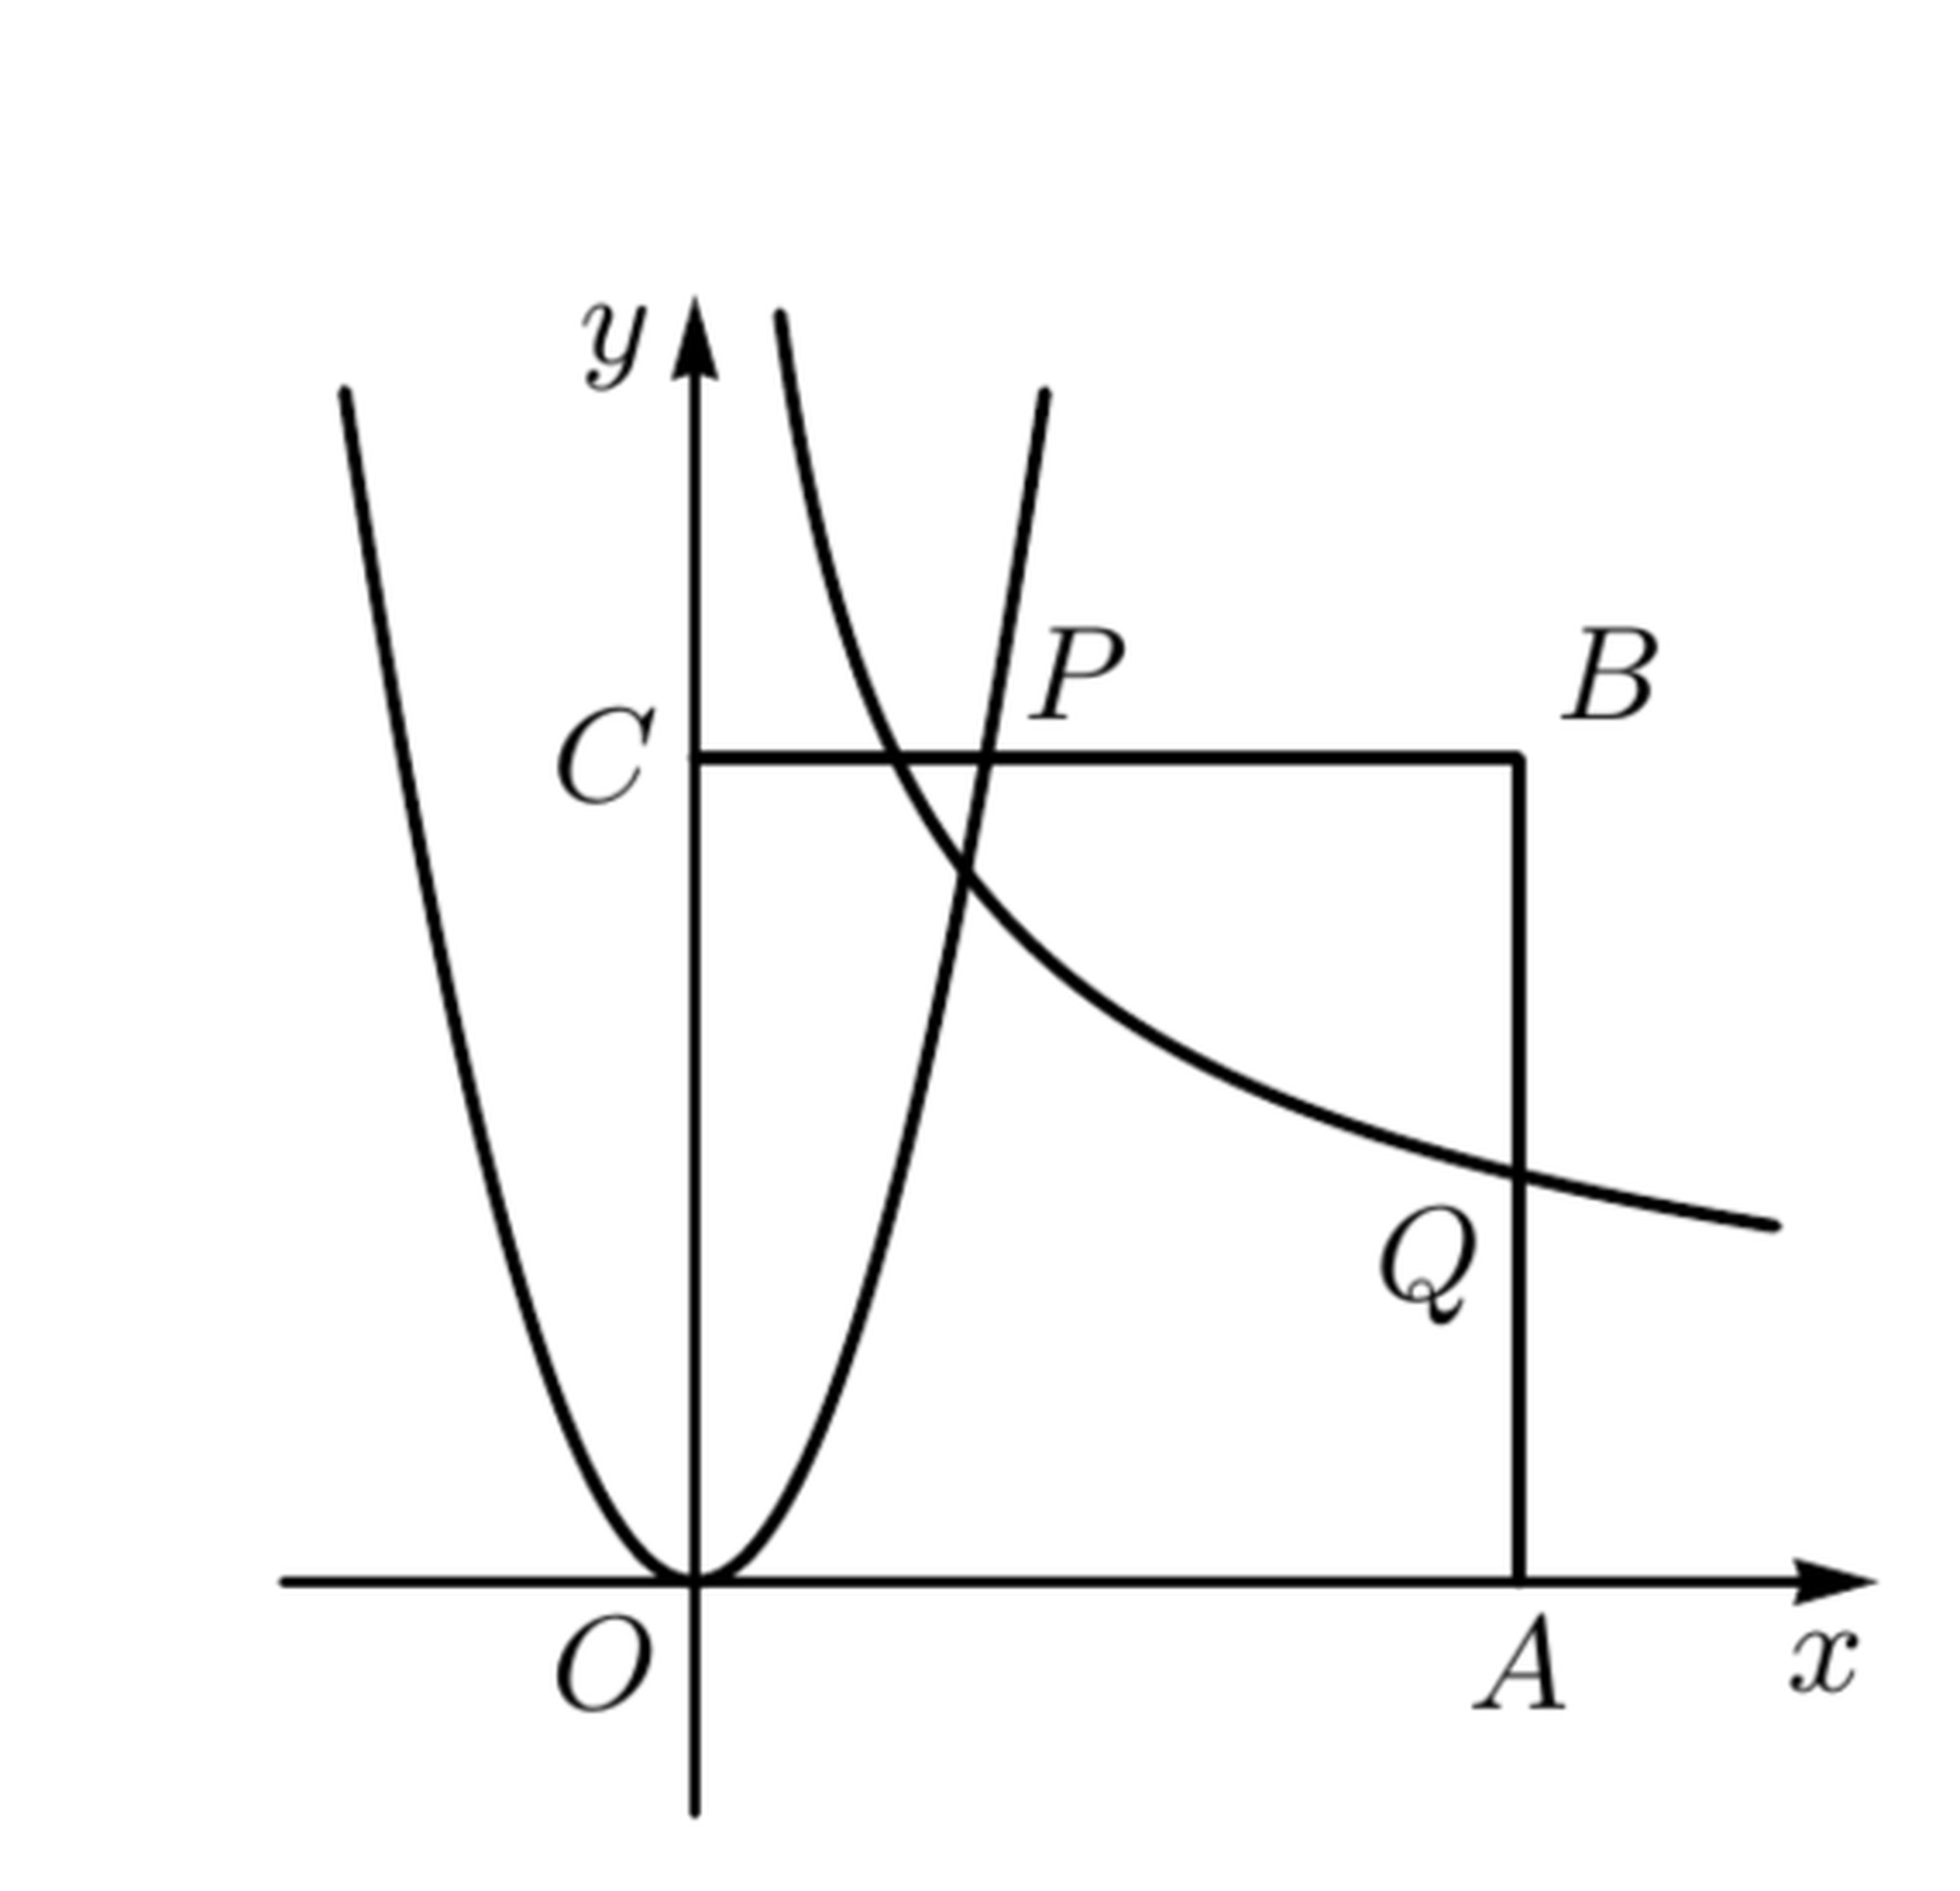
\includegraphics[width=0.40\textwidth]{figures/gao153_q11.png}
\end{center}

\ifanswer
\solbegin
\step{$\lvert AQ\rvert=\dfrac1{\sqrt a}$，$\lvert CP\rvert=\sqrt{\dfrac a5}$，}
\step{于是 $\lvert AQ\rvert+\lvert CP\rvert=\dfrac1{\sqrt a}+\sqrt{\dfrac a5}\geqslant2\sqrt{\dfrac1{\sqrt a}\cdot\sqrt{\dfrac a5}}=\dfrac2{\sqrt[4]{5}}$，}
\step{当且仅当 $\dfrac1{\sqrt a}=\sqrt{\dfrac a5}$，即 $a=\sqrt5$ 时取等号.}
\solend
\fi

% === Q12 === $B\subseteq A$ 带下划线照录、空集 \varnothing；解析 5 行
\item 若集合 $A=\{x\mid1\leqslant x\leqslant100,x\in\Z\}$，集合 $B\subseteq A$，且 $B\ne\varnothing$，记 $W(B)$ 为 $B$ 中元素的最大值与最小值之和，则对所有的 $B$，$W(B)$ 的平均值是\blankline[4.4em].

\ifanswer
\solbegin
\step{对每个非空子集 $B$，令 $B'=\{101-x\mid x\in B\}$，}
\step{则 $W(B')=(101-\min B)+(101-\max B)=202-W(B)$.}
\step{对 $B'$ 再作同样变换即得到 $B$，因此 $B$ 遍历所有非空子集时，}
\step{$B'$ 也恰好遍历所有非空子集.}
\step{设所求平均值为 $m$，则 $m=202-m$，解得 $m=101$.}
\solend
\fi

\end{enumerate}

\bigsec{二、选择题}

\begin{enumerate}
\setcounter{enumi}{12}

% === Q13 === "图像"（像，有亻）照录；解析 2 行，故选 A
\item 设 $a$、$b$ 为常数，若 $0<a<1$，$b>1$，则函数 $y=a^x-b$ 的图像必定不经过\mbox{（\quad）}

\keepwithprev
A. 第一象限\qquad\qquad B. 第二象限\qquad\qquad C. 第三象限\qquad\qquad D. 第四象限

\ifanswer
\solbegin
\step{当 $x>0$ 时，$a^x<1<b$，所以 $y=a^x-b<0$，图像必定不经过第一象限，}
\step{故选 $A$.}
\solend
\fi

% === Q14 === $m\in\Z$、中文弯引号、"图像"照录；解析 3 行，故选 A
\item 已知 $m\in\Z$，则“$m=0$”是“幂函数 $y=x^{m^2-2m-1}$ 的图像与 $x$ 轴及 $y$ 轴均无交点，且关于原点成中心对称”的\mbox{（\quad）}

\keepwithprev
A. 充分不必要条件\qquad\qquad B. 必要不充分条件

C. 充要条件\qquad\qquad D. 既不充分也不必要条件

\ifanswer
\solbegin
\step{图像满足所述条件 $\Leftrightarrow m^2-2m-1$ 为负奇数 $\Leftrightarrow m=0$ 或 $m=2$.}
\step{$m=0$ 能推出所述条件，但所述条件不能推出 $m=0$，因此是充分不必要条件，}
\step{故选 $A$.}
\solend
\fi

% === Q15 === 四选项一行；解析 5 行（跨 03→04 页），故选 D
\item 设 $a>b>1$，$x>1$，则下列不等式正确的是\mbox{（\quad）}

\keepwithprev
A. $a^x<b^x$\qquad B. $x^a<x^b$\qquad C. $\log_a x>\log_b x$\qquad D. $\log_x a>\log_x b$

\ifanswer
\solbegin
\step{$x>1$，幂函数与指数函数的单调性给出 $a^x>b^x$，$x^a>x^b$，A、B 错误.}
\step{$\log_a x=\dfrac{\lg x}{\lg a}<\dfrac{\lg x}{\lg b}=\log_b x$，C 错误.}
\step{对数函数 $y=\log_x t$ 的底数 $x>1$，在 $(0,+\infty)$ 上严格递增，}
\step{所以 $\log_x a>\log_x b$，D 正确.}
\step{故选 $D$.}
\solend
\fi

% === Q16 === $a\in\N$；解析 3 行，故选 C
\item 设 $a\in\N$，则满足不等式 $x^2-a^2x-a^2-1<0$ 的整数 $x$ 的个数不可能是\mbox{（\quad）}

\keepwithprev
A. 1\qquad\qquad B. 50\qquad\qquad C. 100\qquad\qquad D. 2026

\ifanswer
\solbegin
\step{$(x+1)(x-a^2-1)<0\Leftrightarrow-1<x<a^2+1$. 整数解为 $0,1,\cdots,a^2$，共 $a^2+1$ 个.}
\step{$1=0^2+1$，$50=7^2+1$，$2026=45^2+1$，而 $100-1=99$ 不是完全平方数，}
\step{故选 $C$.}
\solend
\fi

\end{enumerate}

\bigsec{三、解答题}

\begin{enumerate}
\setcounter{enumi}{16}

% === Q17 === 补集上划线 \overline{A}、\subseteq 照录；解析 5 行
\item 已知全集 $U=\R$，集合 $A=\{x\mid x^2-x-2\geqslant0\}$，$B=\{x\mid x>-1\}$，$C=\{x\mid a-5<x<a\}$.

(1) 求 $A\cap B$、$A\cup B$；

(2) 若 $\overline{A}\cup C=C$，求实数 $a$ 的取值范围.

\ifanswer
\solbegin
\step{(1) $x^2-x-2=(x+1)(x-2)\geqslant0\Leftrightarrow x\leqslant-1$ 或 $x\geqslant2$，}
\step{所以 $A=(-\infty,-1]\cup[2,+\infty)$，$B=(-1,+\infty)$，}
\step{因此 $A\cap B=[2,+\infty)$，$A\cup B=\R$.}
\step{(2) $\overline{A}=(-1,2)$，于是 $\overline{A}\cup C=C\Leftrightarrow\overline{A}\subseteq C\Leftrightarrow(-1,2)\subseteq(a-5,a)$，}
\step{两区间均为开区间，端点可重合，故 $\begin{cases}a-5\leqslant-1\\a\geqslant2\end{cases}\Leftrightarrow2\leqslant a\leqslant4$.}
\solend
\fi

% === Q18 === 解析 4 行
\item 已知 $a$、$b$、$c$ 都是正数，

(1) 若 $a+b=1$，求证：$\dfrac1a+\dfrac1b\geqslant4$，并指出等号成立的条件；

(2) 若 $a+b+c=1$，求证：三个数 $\dfrac1a$、$\dfrac1b$、$\dfrac1c$ 中至少有一个不小于 3.

\ifanswer
\solbegin
\step{(1) 由 $(a-b)^2\geqslant0$，得 $4ab\leqslant(a+b)^2=1$，所以 $\dfrac1a+\dfrac1b=\dfrac{a+b}{ab}=\dfrac1{ab}\geqslant4$，}
\step{等号成立当且仅当 $a=b$，结合 $a+b=1$，得 $a=b=\dfrac12$.}
\step{(2) 假设三个数 $\dfrac1a$、$\dfrac1b$、$\dfrac1c$ 都小于 3，则 $a>\dfrac13,b>\dfrac13,c>\dfrac13\Rightarrow a+b+c>1$，}
\step{与 $a+b+c=1$ 矛盾，因此三个数中至少有一个不小于 3.}
\solend
\fi

% === Q19 === 题目配图（三版都出）；\needvspace 守卫放 \item 之前；解析 19 行
\needvspace{8cm}
\item 某新建居民小区有一直角三角形绿地，两直角边长分别为 30m 和 40m，打算在其中划出一片区域改造成活动场地，如图所示.

(1) 若划出的区域为正方形，且有两边落在绿地边界上，求此正方形边长；

(2) 若划出的区域为圆形，求圆形区域面积的最大值；

(3) 若划出的区域为矩形（其中至少有一边在边界上），求此矩形面积的最大值.

\begin{center}
% 直角三角形 ABC 绿地示意图取 05 页右上，去粉色水印、去色、4× LANCZOS 放大；三版都出
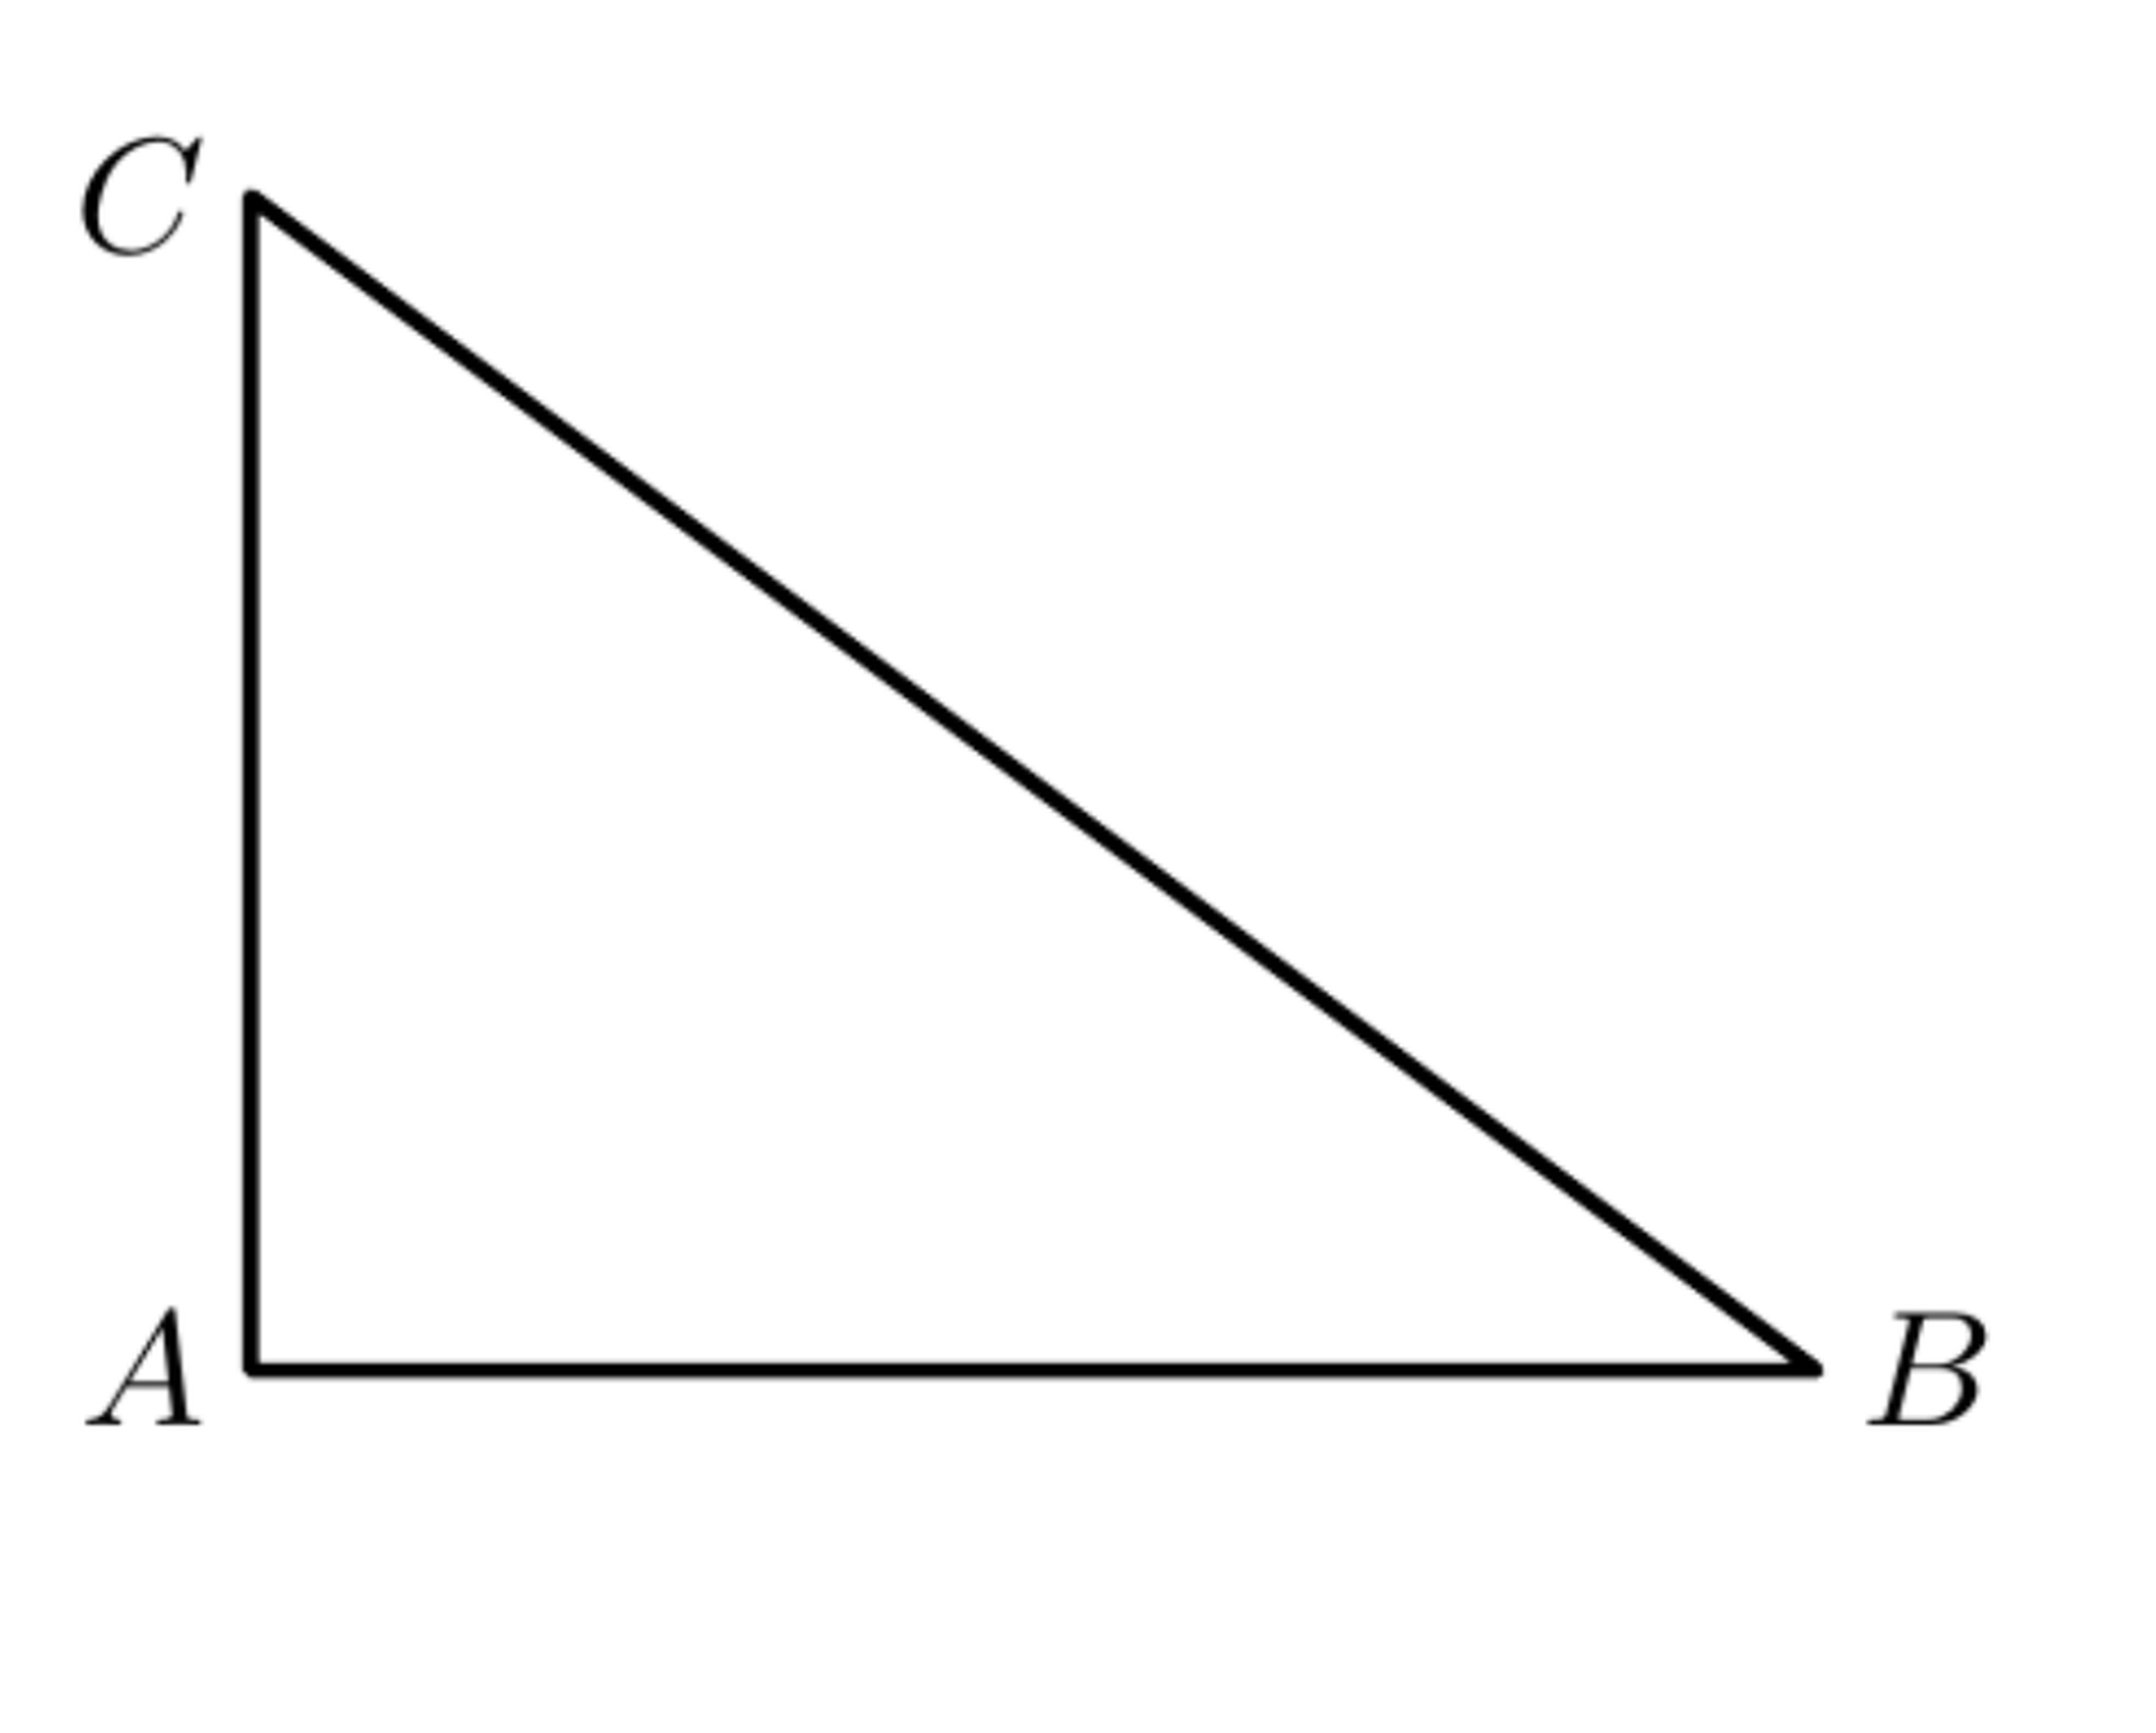
\includegraphics[width=0.34\textwidth]{figures/gao153_q19.png}
\end{center}

\ifanswer
\solbegin
\step{(1) 取 $A(0,0)$、$B(40,0)$、$C(0,30)$，则斜边 $BC$ 所在直线为 $3x+4y=120$.}
\step{正方形落在边界上的两边必分别在两条直角边上.}
\step{设其边长为 $a$m，则对角顶点为 $(a,a)$.}
\step{按题意划出的正方形应尽量大，即对角顶点落在斜边 $BC$ 上，}
\step{因此 $3a+4a=120\Rightarrow a=\dfrac{120}{7}$；}
\step{(2) 斜边长 $BC=\sqrt{30^2+40^2}=50$m，三角形面积为 $600\text{m}^2$.}
\step{设圆的半径为 $r$，圆心到 $AB$、$AC$、$BC$ 的距离分别为 $d_1,d_2,d_3$，}
\step{则三者均不小于 $r$. 连接圆心与三个顶点，}
\step{得 $600=\dfrac12(40d_1+30d_2+50d_3)\geqslant\dfrac12(40+30+50)r=60r$，所以 $r\leqslant10$.}
\step{取三角形的内切圆时等号成立，圆形区域面积的最大值为 $100\pi\text{m}^2$.}
\step{(3) 任取矩形落在绿地边界上的一边，以其所在直线为横轴.}
\step{设相应三角形底边长为 $L$、高为 $H$，则 $LH=1200$.}
\step{取三角形顶点坐标为 $(0,0)$、$(L,0)$、$(p,H)$.}
\step{在高度 $t$ 处，两腰上的点的横坐标分别为 $\dfrac{pt}{H}$、$L+\dfrac{(p-L)t}{H}$，}
\step{因此，高为 $t$ 的矩形，其底边长不超过 $L\left(1-\dfrac tH\right)$，}
\step{面积满足 $S\leqslant Lt\left(1-\dfrac tH\right)=\dfrac LH\left[\dfrac{H^2}{4}-\left(t-\dfrac H2\right)^2\right]\leqslant\dfrac{LH}{4}=300$，}
\step{在原坐标系中，取矩形顶点为 $(0,0)$、$(20,0)$、$(20,15)$、$(0,15)$，}
\step{其中 $3\times20+4\times15=120$，矩形完全位于绿地内，面积为 $300\text{m}^2$，}
\step{达到最大值.}
\solend
\fi

% === Q20 === $g(x)$ 定义照录；解析 14 行
\item 已知 $a>0$ 且 $a\ne1$，设 $f(x)=\log_a(x^2-a^2)$，$g(x)=2\log_a(x-ak)$.

(1) 求函数 $y=f(x)$ 的定义域；

(2) 若 $k=2$，求不等式 $f(x)>g(x)$ 的解集；

(3) 若“存在实数 $x$，使得 $f(x)=g(x)$”为真命题，求实数 $k$ 的取值范围.

\ifanswer
\solbegin
\step{(1) $x^2-a^2>0\Leftrightarrow x<-a$ 或 $x>a$，定义域为 $(-\infty,-a)\cup(a,+\infty)$.}
\step{(2) 两函数均有意义时，$x>2a$，且 $g(x)=\log_a(x-2a)^2$.}
\step{当 $a>1$ 时，$f(x)>g(x)\Leftrightarrow x^2-a^2>(x-2a)^2\Leftrightarrow x>\dfrac{5a}{4}$，}
\step{结合 $x>2a$，解集为 $(2a,+\infty)$.}
\step{当 $0<a<1$ 时，$f(x)>g(x)\Leftrightarrow x^2-a^2<(x-2a)^2\Leftrightarrow x<\dfrac{5a}{4}$，}
\step{与 $x>2a$ 矛盾，解集为 $\varnothing$.}
\step{(3) 在 $x^2-a^2>0$ 且 $x-ak>0$ 的条件下，}
\step{$f(x)=g(x)\Leftrightarrow x^2-a^2=(x-ak)^2\Leftrightarrow2akx=a^2(1+k^2)$，}
\step{当 $k=0$ 时，上式不成立；}
\step{当 $k\ne0$ 时，$x=\dfrac{a(1+k^2)}{2k}$，}
\step{于是 $x-ak=\dfrac{a(1-k^2)}{2k}>0\Leftrightarrow k<-1$ 或 $0<k<1$，}
\step{对上述 $k$，所取的 $x$ 同时满足 $x^2-a^2=(x-ak)^2>0$，}
\step{两函数均有意义且函数值相等.}
\step{因此，$k$ 的取值范围为 $(-\infty,-1)\cup(0,1)$.}
\solend
\fi

% === Q21 === 中文弯引号、复杂式照录；解析 23 行（跨 08→09 页）
\item 若实数 $x$、$y$、$m$ 满足 $\lvert x-m\rvert<\lvert y-m\rvert$，则称 $x$ 比 $y$ 接近 $m$.

(1) 若 $2x$ 比 $x-2$ 更接近 1，求实数 $x$ 的取值范围；

(2) 若 $x$ 比 $y$ 接近 $m$，证明：“$x>y$” 的充要条件是 “$x+y<2m$”；

(3) 已知 $x>0$，$y>0$ 且 $x\ne y$. 设 $p=\dfrac{x^2+y^2}{xy}$，若对于任意的 $x$、$y$，命题 “$p$ 比 $p^2-3p+4$ 接近 $m$” 恒成立，求实数 $m$ 的取值范围.

\ifanswer
\solbegin
\step{(1) $\lvert2x-1\rvert<\lvert x-3\rvert\Leftrightarrow(2x-1)^2<(x-3)^2\Leftrightarrow(x+2)(3x-4)<0$，}
\step{解得 $-2<x<\dfrac43$，实数 $x$ 的取值范围为 $\left(-2,\dfrac43\right)$.}
\step{(2) 因为 $x$ 比 $y$ 接近 $m$，所以 $\lvert x-m\rvert<\lvert y-m\rvert$，则 $\lvert x-m\rvert^2<\lvert y-m\rvert^2$，}
\step{即 $(x-m)^2<(y-m)^2$，即 $(x-m)^2-(y-m)^2<0$，}
\step{即得 $(x-y)(x+y-2m)<0$，}
\step{则由 $x+y<2m$，得 $x+y-2m<0$，}
\step{故 $x-y>0$，即 $x>y$，充分性成立；}
\step{当 $x>y$ 时，$x-y>0$，结合 $(x-y)(x+y-2m)<0$，得 $x+y-2m<0$，}
\step{即 $x+y<2m$，必要性成立；}
\step{故“$x>y$” 的充要条件是 “$x+y<2m$”；}
\step{(3) $x>0$，$y>0$ 且 $x\ne y$. 则 $p=\dfrac{x^2+y^2}{xy}=\dfrac xy+\dfrac yx>2\sqrt{\dfrac xy\cdot\dfrac yx}=2$，}
\step{由于对于任意的 $x$、$y$，命题 “$p$ 比 $p^2-3p+4$ 接近 $m$” 恒成立，}
\step{故 $\lvert p-m\rvert<\lvert(p^2-3p+4)-m\rvert$ 对 $\forall p>2$ 恒成立，}
\step{即得 $(p-m)^2<(p^2-3p+4-m)^2$，}
\step{即 $(p^2-3p+4-m)^2-(p-m)^2>0$，}
\step{得 $(p^2-4p+4)(p^2-2p+4-2m)>0$，}
\step{即 $(p-2)^2(p^2-2p+4-2m)>0$，由于 $p>2$，故 $(p-2)^2>0$，}
\step{故 $p^2-2p+4-2m>0$ 对 $\forall p>2$ 恒成立，}
\step{即 $2m<p^2-2p+4$ 对 $\forall p>2$ 恒成立，}
\step{由于 $p^2-2p+4=(p-1)^2+3$，此时 $p^2-2p+4$ 在 $(2,+\infty)$ 上严格增，}
\step{故 $(p-1)^2+3>(2-1)^2+3=4$，故 $2m\leqslant4$，解得 $m\leqslant2$，}
\step{即实数 $m$ 的取值范围是 $(-\infty,2]$.}
\solend
\fi

\end{enumerate}

\end{document}
"
% 紧凑版：xelatex "\def\iscompact{1}% 高一153_闵行中学文绮中学_期中.tex
%   —— 高一上数学"2026-2027 年闵行中学文绮中学高一上期中"（试卷版/答案版/紧凑版）
% 试卷版：xelatex 高一153_闵行中学文绮中学_期中.tex
% 答案版：xelatex "\def\isanswer{1}\input{高一153_闵行中学文绮中学_期中.tex}"
% 紧凑版：xelatex "\def\iscompact{1}\input{高一153_闵行中学文绮中学_期中.tex}"
%
% ① 原始材料：微信公众号"魔都数学加油站"文章，连载"27学年高一153"，原文标题
% "27学年高一153——2026-2027年上海市闵行中学文绮中学高一上期中"；
% 原文链接：https://mp.weixin.qq.com/s/rEtS-92cDR6JKgY2b5DRfg 。
% 正文为 9 张 PNG 页（01/02/06/07/08/09 为 2560×3620，03/04/05 为 4762×6735，
% 同一篇各页分辨率混排，逐页按各自分辨率裁图核对，别按预览比例换算裁框）。
% 体例：讲评版——填空 3—12（10 题）、选择 13—16（4 题）、解答 17—21（5 题），
% 共 19 题，自第 3 题起编；**全 19 题均印【解析】**（逐题核实，见 ② ②）。
% 题目、答案、解析均据原图转录；卷面粉红色水印"魔都数学加油站"及公众号页脚未录入。
% 全卷插图清单（逐页通读 9 页确认）：2 幅，均为题目配图、三版都出——
%   · Q11 正方形 OABC 曲线图（02 页右下：$y=5x^2$ 与 $y=x^{-\frac12}$ 两条曲线、
%     坐标轴、O/A/B/C/P/Q、正方形），裁 figures/gao153_q11.png；
%   · Q19 直角三角形 ABC 绿地示意图（05 页右上，直角在 A），
%     裁 figures/gao153_q19.png；
%   两图均去粉色水印、去色、4× LANCZOS 放大；Q11 图左上角题干残字"函"已裁白。
%   其余各页逐页确认无其它题目配图、无解析内配图、无表格；09 页下半仅水印、无正文。
%
% 卷首标题：原卷印作"2026-2027 年闵行中学文绮中学高一上期中"，年份区间按全稿惯例排 en dash；
% 原卷卷面未印副标题，本稿按同期中卷知识模块口径补出"集合与常用逻辑用语、不等式、函数"。
%
% ② 与原卷的排版差异：
%   ① 原文从第 3 题起，本稿保留原题号；共 19 题三节，解答题 5 题到 21；
%   ② 全 19 题均印【解析】、用 \solbegin…\solend，无只印【答案】或答案印括号内的题；
%      四道选择题答案在解析末句"故选 A／A／D／C"（Q13—Q16，逐个放大复核）、
%      括号 \mbox{（\quad）} 留空、不另提 \ans{}；答案版【答案】/【解析】标记数
%      = 19 = 全卷题数；
%   ③ 原卷卷面未印副标题，本稿按知识模块口径补出；
%   ④ 原卷填空横线按全稿惯例排 \blankline[4.4em]；选择题括号排 \mbox{（\quad）}、
%      四道选择题的选项段前按惯例各加 \keepwithprev；解答题不留作答区、不加
%      \anspace（原卷为讲评版，109—113 起全稿不用 \anspace）；
%   ⑤ 数集：Q3"$x\in R$"、Q5"解集为 R"、Q10"$x\in N$"、Q12"$x\in Z$"与
%      "$m\in Z$"、Q14"$m\in Z$"、Q16"$a\in N$"、Q17"全集 $U=R$"、
%      Q19 无、Q21 无——原卷印斜体或正体粗体 R/N/Z，按全稿惯例归一
%      \R／\N／\Z；绝对值排 \lvert…\rvert（Q5、Q11、Q21），集合描述竖线排 \mid
%      （Q3、Q10、Q17、Q20），不等号按全稿惯例排 \leqslant／\geqslant；
%      补集照原卷上划线排 \overline{A}（Q17 题干 (2)＋解析 (2)）；
%      空集 \varnothing（Q12 题干、Q20 解析 (2)）；子集 3 处均印带下划线 ⊆、
%      照录 \subseteq（Q10 $A\subseteq U$、Q12 $B\subseteq A$、Q17 $(-1,2)\subseteq(a-5,a)$），
%      本卷无单线 \subset 用例；
%   ⑥ 判别式：逐页通读 9 页，本卷无一元二次判别式 Δ/△ 算式，故无 Δ/△ 混用可照录；
%      Q11 图里有几何正方形 OABC（非三角形符号），无 △ABC 用例；
%   ⑦ 中文弯引号照录：Q14"$m=0$"与"幂函数…关于原点成中心对称"、
%      Q20"存在实数 $x$，使得 $f(x)=g(x)$"、Q21"$x>y$"与"$x+y<2m$"、
%      "$p$ 比 $p^2-3p+4$ 接近 $m$"（引号外留空格按原卷）；
%      注释里一律 ASCII 引号；数学式内 CJK 用 \text{}；
%   ⑧ "图像／图象"逐处放大核：全卷 3 处均印"图像"（像，有亻）——
%      Q13 题干与解析、Q14 题干与解析；Q19 题干写"如图所示"（非"图像"），
%      逐处照录未统一；子题标号 (1)(2)(3) 半角括号照录；圈数字本卷无用例；
%   ⑨ 半角逗号在数学组之间是全稿惯例、非笔误，逐处照录（Q3 $x\in R$、
%      Q10 $a_1,a_2$、Q19 $A(0,0)$、$d_1,d_2,d_3$、Q21 $a>\frac13,b>\frac13$ 等）；
%      行末西文句点 ASCII `.`；行中全角逗号／顿号照录（Q19"30m 和 40m"、
%      Q21"实数 $x$、$y$、$m$"）；
%   ⑩ 复杂式照录别简化：Q3 $y=x^{-2}$、Q11 $y=x^{-\frac12}$ 与
%      $\frac{2}{\sqrt[4]{5}}$、Q8 $\frac{2b}{a+1-b}$、Q9 cases 块、
%      Q10 $525=5\times105$、Q16 $a^2+1$、Q19 $S\leqslant Lt(1-\frac tH)$
%      与 $L+\frac{(p-L)t}{H}$、Q20 $2akx=a^2(1+k^2)$ 与 $\frac{a(1+k^2)}{2k}$、
%      Q21 $(p^2-4p+4)(p^2-2p+4-2m)>0$；
%      \left…\right 不得拆到不同 $…$ 组（Q17 $\left\{x\mid\cdots\right\}$、
%      Q19 $\left[\frac{H^2}{4}-\left(t-\frac H2\right)^2\right]$、
%      Q21 $\left(-2,\frac43\right)$ 等）；cases 块一律 \begin{cases}…\end{cases}；
%   ⑪ 一条 \step = 原卷解析的一个印刷行，cases 块整体算一个印刷行；别并折行、
%      别拆行。Q10 六行、Q19 十九行、Q20 十四行、Q21 二十二行均按印刷行逐条断，
%      不丢行；
%   ⑫ 配图：Q11／Q19 题目配图（三版都出）放 \item 内题干之后 \begin{center}，
%      各用 \needvspace{8cm} 守卫把整块推走，**守卫放在 \item 之前**
%      （见 高一145 Q14/Q20 成例与切页审计 B 类坑）；
%   ⑬ 原卷解析内无红色"法一／法二"之类小标题，故本卷无 \stepm；红色水印
%      "魔都数学加油站"不录入；
%   ⑭ 跨页续印按题合并：见 ⑥；
%
% ③ 行数复核：一条 \step = 原卷解析的一个印刷行，cases 块作一个印刷行计。
%   逐题数（主会话逐页核对定稿）：Q3：1；Q4：2；Q5：2；Q6：2；Q7：1；
%   Q8：1；Q9：2；Q10：6；Q11：3；Q12：5；Q13：2；Q14：3；Q15：5；
%   Q16：3；Q17：5；Q18：4；Q19：19；Q20：14；Q21：22。
%   合计 102 条 \step（本卷无 \stepm），与原卷逐题印刷行相等。全卷 19 题
%   均设 \solbegin…\solend，答案版【答案】/【解析】标记数 = 19 = 全卷题数。
%
% ④ 判别式／子集符号结论（逐处放大原图照录、不得统一，主会话像素级复核）：
%   判别式：逐页通读 9 页，本卷无一元二次判别式算式（Q7 用韦达定理、
%      Q16 用因式分解、Q20 用对数方程，均不写 Δ/△），故无 Δ/△ 混用可照录
%      （"高 \Delta／扁 \triangle"口径备查，参照 高一142／151／152 头注）；
%      本卷无几何三角形符号用例。
%   子集：Q10 题干"$A\subseteq U$"、Q12 题干"$B\subseteq A$"、Q17 解析 (2)
%      "$(-1,2)\subseteq(a-5,a)$"共 3 处，逐处放大确认均印带下划线 ⊆、
%      照录 \subseteq；本卷未见单线 ⊂（\subset）之对应处。
%      补集上划线 \overline{A}（Q17）、空集 \varnothing（Q12 题干、Q20 解析 (2)）；
%      数集 \R／\N／\Z 归一见 ② ⑤。
%
% ⑤ 存疑照录（放大原图确认，照录未改、正文对应处另有 % 注）：
%   1. Q3 集合 $B=\{(x,y)\mid y=x^{-2},x\in\R\}$ 原卷题干径写 $x\in\R$
%      （$x=0$ 处无意义），解析自行注明 $x\ne0$，照录未改。
%   2. Q10 解析"$U$ 中共有 $525=5\times105$ 个连续整数"与尾行
%      "取 $U$ 中除以 5 余 1 或 2 的全部元素及元素 5"逐字照录（放大 02 页
%      /tmp/gao153/z/zoom/q10_pick.png 确认是"元素 5"，非"元素 9"）。
%   3. Q11 第二个函数原卷印 $y=x^{-\frac12}$（负二分之一次幂，非 $x^2$），
%      放大 02 页 /tmp/gao153/z/zoom/q11_exp.png 确认，照录未改；
%      $|AQ|=\frac1{\sqrt a}$ 与之自洽。
%   4. Q19 (3) 解析"在高度 $t$ 处，两腰上的点的横坐标分别为 $\frac{pt}{H}$、
%      $L+\frac{(p-L)t}{H}$"，放大 06 页确认，照录未简化。
%   5. Q20 (2) 解析"$g(x)=\log_a(x-2a)^2$"（真数整体平方），
%      与 $g(x)=2\log_a(x-ak)$ 在 $k=2$ 时一致，照录未改。
%   6. Q21 (3) 解析"得 $(p^2-4p+4)(p^2-2p+4-2m)>0$"与
%      "故 $(p-1)^2+3>(2-1)^2+3=4$，故 $2m\leqslant4$"照录未改
%      （放大 09 页 /tmp/gao153/z/zoom/q21_factor.png 确认）。
%   7. "图像／图象"全卷 3 处均印"图像"（像，有亻）逐处照录；
%      本卷无判别式 Δ/△ 用例（见 ④）。
%   全卷除此 7 类外未发现其它笔误／自相矛盾处；19 题均印【解析】、
%   无只印【答案】或答案印括号内的题（见 ② ②）。
%
% ⑥ 跨页续印按题合并说明（逐页核实定稿）：Q3—Q5 题干＋解析在 01 页；
%   Q6—Q8 题干＋解析在 01 页下半（Q8 解析续 02 页顶）；Q9 题干＋解析、
%   Q10 题干＋解析首 2 行在 02 页上半，Q10 解析余 4 行在 02 页下半；
%   Q11 题干＋配图＋解析、Q12 题干＋解析 5 行在 02 页下半—03 页上半；
%   "二、选择题"标题在 03 页中部；Q13 题干＋选项＋解析在 03 页下半；
%   Q14 题干＋选项＋解析、Q15 题干＋选项＋解析首行在 03 页下半—04 页顶；
%   Q15 解析余 4 行、Q16 题干＋选项＋解析在 04 页上半；"三、解答题"
%   标题在 04 页下半；Q17 题干＋两问＋解析 5 行在 04 页下半—05 页顶；
%   Q18 题干＋两问＋解析 4 行、Q19 题干（含配图）＋三问在 05 页；
%   Q19 解析 (1)(2) 9 行在 05 页下半，解析 (3) 前 5 行在 06 页上半、
%   余 4 行在 06 页下半；Q20 题干＋三问在 06 页下半，解析 (1)(2)(3)
%   前 6 行在 07 页上半、(3) 余 8 行在 07 页下半；Q21 题干＋三问在
%   07 页末，解析 (1)(2) 10 行在 08 页上半—下半，解析 (3) 前 4 行在
%   08 页下半、余 9 行续 09 页上半，末行"即实数 $m$ 的取值范围是
%   $(-\infty,2]$"为全卷收尾（09 页下半仅水印、无正文）。
%   本稿按题连排，不丢行、不并折行；全卷末题为第 21 题，无附加题节。
%
\documentclass[a4paper,11pt]{article}
\usepackage{common}

\begin{document}

\examtitlest[3]{2026--2027 年闵行中学文绮中学高一上期中}{集合与常用逻辑用语、不等式、函数}

\bigsec{一、填空题}

\begin{enumerate}
\setcounter{enumi}{2}

% === Q3 === 集合描述竖线 \mid；$y=x^{-2}$ 照录；解析 1 行
\item 已知 $A=\{(x,y)\mid y=x^3,x\in\R\}$，$B=\{(x,y)\mid y=x^{-2},x\in\R\}$，则 $A\cap B=$\blankline[4.4em].

\ifanswer
\solbegin
\step{$x^3=x^{-2}\ (x\ne0)\Leftrightarrow x^5=1\Leftrightarrow x=1$，此时 $y=1$，所以 $A\cap B=\{(1,1)\}$.}
\solend
\fi

% === Q4 === 解析 2 行
\item 若关于 $x$ 的不等式 $\dfrac{x-a}{x+1}>0$ 的解集为 $(-\infty,-1)\cup(4,+\infty)$，则实数 $a=$\blankline[4.4em].

\ifanswer
\solbegin
\step{关于 $x$ 的不等式 $\dfrac{x-a}{x+1}>0$ 即 $(x+1)(x-a)>0$.}
\step{再由它的解集为 $(-\infty,-1)\cup(4,+\infty)$，得 $-1$ 和 4 是 $(x+1)(x-a)=0$ 的两个实数根，故 $a=4$.}
\solend
\fi

% === Q5 === 绝对值 \lvert…\rvert；解析 2 行
\item 若关于 $x$ 的不等式 $\lvert x+1\rvert+\lvert x-2\rvert>m$ 的解集为 $\R$，则实数 $m$ 的取值范围是\blankline[4.4em].

\ifanswer
\solbegin
\step{$\lvert x+1\rvert+\lvert x-2\rvert\geqslant\lvert(x+1)-(x-2)\rvert=3$，当且仅当 $-1\leqslant x\leqslant2$ 时取等号，}
\step{因此 $m<3$.}
\solend
\fi

% === Q6 === 解析 2 行
\item 已知指数函数 $y=a^x$（$a>1$）在区间 $[-1,1]$ 上的最大值比最小值大 $\dfrac32$，则实数 $a=$\blankline[4.4em].

\ifanswer
\solbegin
\step{$a>1$，指数函数在 $[-1,1]$ 上严格增，故 $a-\dfrac1a=\dfrac32\Leftrightarrow(a-2)(2a+1)=0$.}
\step{结合 $a>1$，得 $a=2$.}
\solend
\fi

% === Q7 === 韦达定理；解析 1 行
\item 已知关于 $x$ 的一元二次方程 $x^2+px+2p=0$ 的两个实数根分别为 $x_1$、$x_2$，且 $(x_1+1)(x_2+1)=0$，则 $p=$\blankline[4.4em].

\ifanswer
\solbegin
\step{$0=(x_1+1)(x_2+1)=x_1x_2+x_1+x_2+1=2p-p+1=p+1\Rightarrow p=-1$.}
\solend
\fi

% === Q8 === 换底公式；解析 1 行
\item 已知 $10^a=3$，$\lg5=b$，则 $\log_6 25=$\blankline[4.4em]（用关于 $a,b$ 的关系式表示）.

\ifanswer
\solbegin
\step{$\lg3=a$，$\lg2=1-b$，所以 $\log_6 25=\dfrac{\lg25}{\lg6}=\dfrac{2b}{a+1-b}$.}
\solend
\fi

% === Q9 === cases 块整体算一个印刷行；解析 2 行
\item 已知 $A=[2,5]$，若对任意 $x\in A$，总有 $\dfrac{k}{x}\in A$，则正数 $k=$\blankline[4.4em].

\ifanswer
\solbegin
\step{$k>0$，当 $x\in[2,5]$ 时，$\dfrac{k}{x}$ 的取值范围为 $\left[\dfrac k5,\dfrac k2\right]$，}
\step{因此 $\begin{cases}\dfrac k5\geqslant2\\\dfrac k2\leqslant5\end{cases}\Leftrightarrow10\leqslant k\leqslant10\Leftrightarrow k=10$.}
\solend
\fi

% === Q10 === $A\subseteq U$ 带下划线照录；解析 6 行
\item 已知集合 $U=\{x\mid4\leqslant x\leqslant528,x\in\N\}$，$A=\{a_1,a_2,a_3,\cdots,a_n\}$，且 $A\subseteq U$. 如果集合 $A$ 中的任意两个不同元素之和都不能被 5 整除，则正整数 $n$ 的最大值为\blankline[4.4em].

\ifanswer
\solbegin
\step{$U$ 中共有 $525=5\times105$ 个连续整数，按除以 5 的余数分成五类，}
\step{每类均有 105 个元素.}
\step{余数为 1,4 的两类不能同时选取，余数为 2,3 的两类也不能同时选取，}
\step{余数为 0 的一类最多选 1 个，因此 $n\leqslant105+105+1=211$.}
\step{取 $U$ 中除以 5 余 1 或 2 的全部元素及元素 5，}% 放大 02 页确认是「元素 5」（非 9），照录未改（见 ⑤ 2）
\step{任意两个不同元素之和均不能被 5 整除，此时 $n=211$，最大值为 211.}
\solend
\fi

% === Q11 === 题目配图（三版都出）；\needvspace 守卫放 \item 之前；$y=x^{-\frac12}$ 照录；解析 3 行
\needvspace{8cm}
\item 如图，已知正方形 $OABC$，其中 $OA=a$（$a>1$），函数 $y=5x^2$ 交 $BC$ 于点 $P$，函数 $y=x^{-\frac12}$ 交 $AB$ 于点 $Q$，当 $\lvert AQ\rvert+\lvert CP\rvert$ 最小时，$a$ 的值为\blankline[4.4em].

\begin{center}
% 正方形 OABC 与两条曲线图取 02 页右下，去粉色水印、去色、4× LANCZOS 放大；三版都出
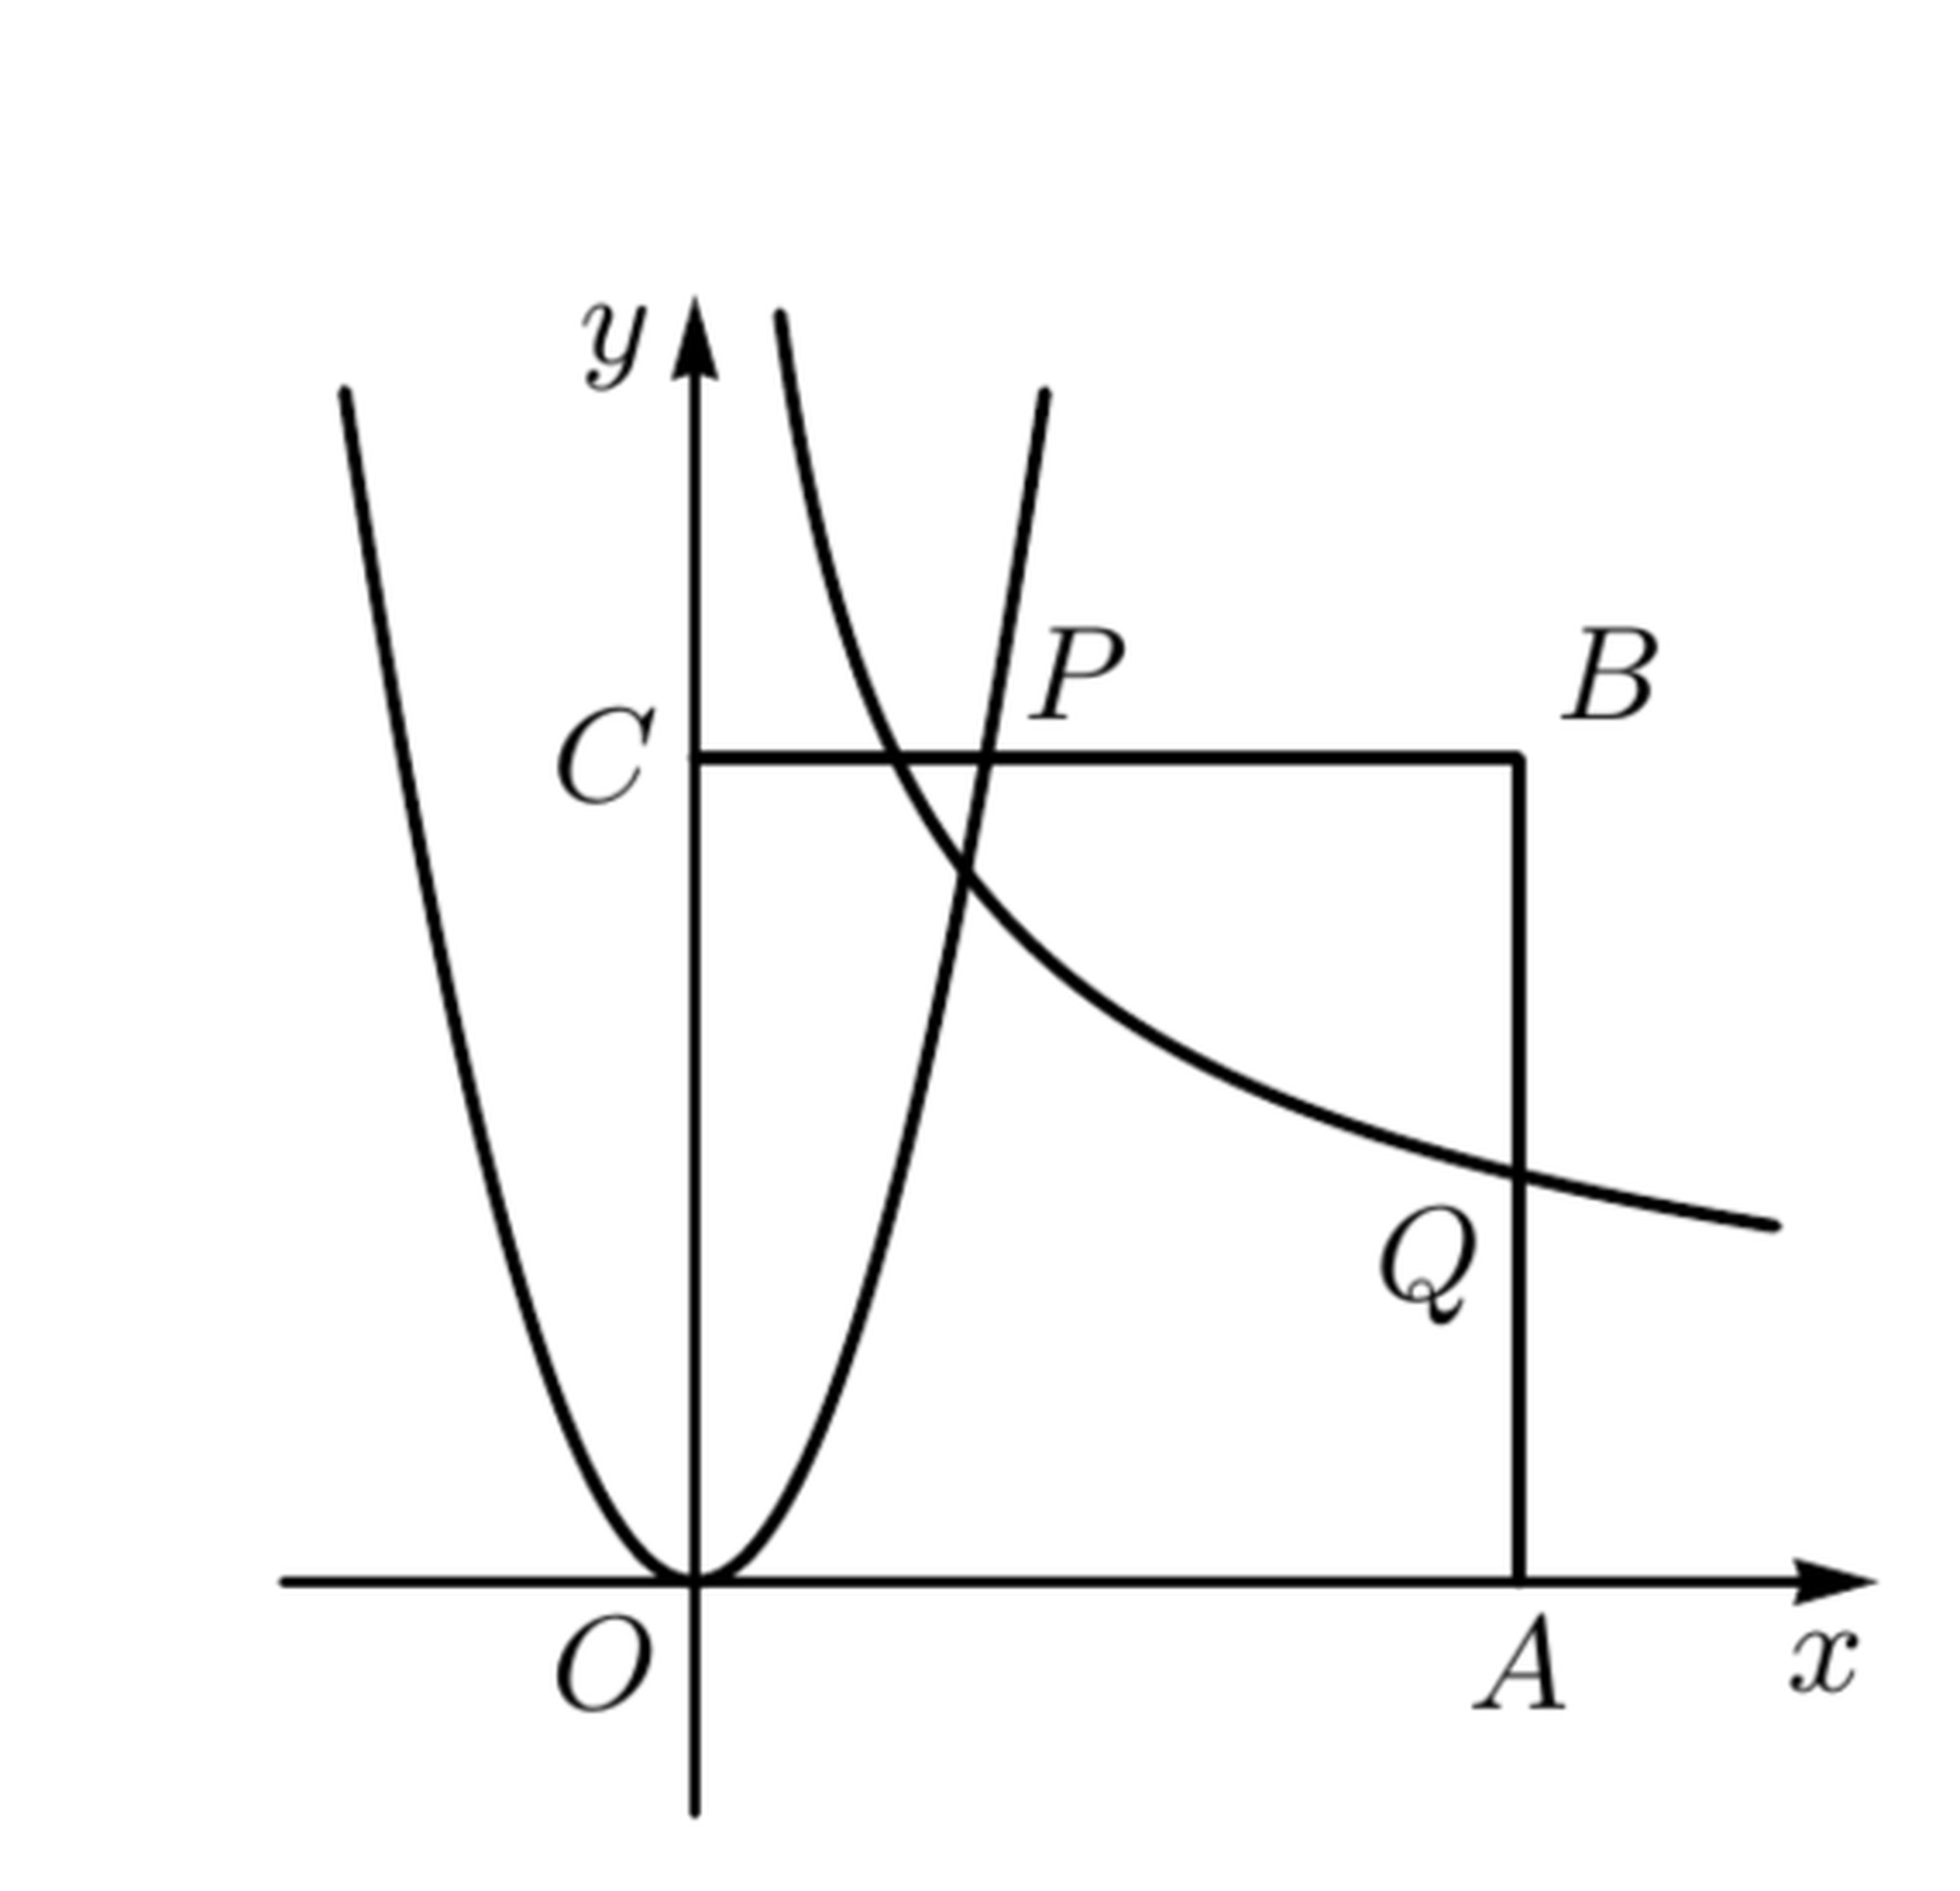
\includegraphics[width=0.40\textwidth]{figures/gao153_q11.png}
\end{center}

\ifanswer
\solbegin
\step{$\lvert AQ\rvert=\dfrac1{\sqrt a}$，$\lvert CP\rvert=\sqrt{\dfrac a5}$，}
\step{于是 $\lvert AQ\rvert+\lvert CP\rvert=\dfrac1{\sqrt a}+\sqrt{\dfrac a5}\geqslant2\sqrt{\dfrac1{\sqrt a}\cdot\sqrt{\dfrac a5}}=\dfrac2{\sqrt[4]{5}}$，}
\step{当且仅当 $\dfrac1{\sqrt a}=\sqrt{\dfrac a5}$，即 $a=\sqrt5$ 时取等号.}
\solend
\fi

% === Q12 === $B\subseteq A$ 带下划线照录、空集 \varnothing；解析 5 行
\item 若集合 $A=\{x\mid1\leqslant x\leqslant100,x\in\Z\}$，集合 $B\subseteq A$，且 $B\ne\varnothing$，记 $W(B)$ 为 $B$ 中元素的最大值与最小值之和，则对所有的 $B$，$W(B)$ 的平均值是\blankline[4.4em].

\ifanswer
\solbegin
\step{对每个非空子集 $B$，令 $B'=\{101-x\mid x\in B\}$，}
\step{则 $W(B')=(101-\min B)+(101-\max B)=202-W(B)$.}
\step{对 $B'$ 再作同样变换即得到 $B$，因此 $B$ 遍历所有非空子集时，}
\step{$B'$ 也恰好遍历所有非空子集.}
\step{设所求平均值为 $m$，则 $m=202-m$，解得 $m=101$.}
\solend
\fi

\end{enumerate}

\bigsec{二、选择题}

\begin{enumerate}
\setcounter{enumi}{12}

% === Q13 === "图像"（像，有亻）照录；解析 2 行，故选 A
\item 设 $a$、$b$ 为常数，若 $0<a<1$，$b>1$，则函数 $y=a^x-b$ 的图像必定不经过\mbox{（\quad）}

\keepwithprev
A. 第一象限\qquad\qquad B. 第二象限\qquad\qquad C. 第三象限\qquad\qquad D. 第四象限

\ifanswer
\solbegin
\step{当 $x>0$ 时，$a^x<1<b$，所以 $y=a^x-b<0$，图像必定不经过第一象限，}
\step{故选 $A$.}
\solend
\fi

% === Q14 === $m\in\Z$、中文弯引号、"图像"照录；解析 3 行，故选 A
\item 已知 $m\in\Z$，则“$m=0$”是“幂函数 $y=x^{m^2-2m-1}$ 的图像与 $x$ 轴及 $y$ 轴均无交点，且关于原点成中心对称”的\mbox{（\quad）}

\keepwithprev
A. 充分不必要条件\qquad\qquad B. 必要不充分条件

C. 充要条件\qquad\qquad D. 既不充分也不必要条件

\ifanswer
\solbegin
\step{图像满足所述条件 $\Leftrightarrow m^2-2m-1$ 为负奇数 $\Leftrightarrow m=0$ 或 $m=2$.}
\step{$m=0$ 能推出所述条件，但所述条件不能推出 $m=0$，因此是充分不必要条件，}
\step{故选 $A$.}
\solend
\fi

% === Q15 === 四选项一行；解析 5 行（跨 03→04 页），故选 D
\item 设 $a>b>1$，$x>1$，则下列不等式正确的是\mbox{（\quad）}

\keepwithprev
A. $a^x<b^x$\qquad B. $x^a<x^b$\qquad C. $\log_a x>\log_b x$\qquad D. $\log_x a>\log_x b$

\ifanswer
\solbegin
\step{$x>1$，幂函数与指数函数的单调性给出 $a^x>b^x$，$x^a>x^b$，A、B 错误.}
\step{$\log_a x=\dfrac{\lg x}{\lg a}<\dfrac{\lg x}{\lg b}=\log_b x$，C 错误.}
\step{对数函数 $y=\log_x t$ 的底数 $x>1$，在 $(0,+\infty)$ 上严格递增，}
\step{所以 $\log_x a>\log_x b$，D 正确.}
\step{故选 $D$.}
\solend
\fi

% === Q16 === $a\in\N$；解析 3 行，故选 C
\item 设 $a\in\N$，则满足不等式 $x^2-a^2x-a^2-1<0$ 的整数 $x$ 的个数不可能是\mbox{（\quad）}

\keepwithprev
A. 1\qquad\qquad B. 50\qquad\qquad C. 100\qquad\qquad D. 2026

\ifanswer
\solbegin
\step{$(x+1)(x-a^2-1)<0\Leftrightarrow-1<x<a^2+1$. 整数解为 $0,1,\cdots,a^2$，共 $a^2+1$ 个.}
\step{$1=0^2+1$，$50=7^2+1$，$2026=45^2+1$，而 $100-1=99$ 不是完全平方数，}
\step{故选 $C$.}
\solend
\fi

\end{enumerate}

\bigsec{三、解答题}

\begin{enumerate}
\setcounter{enumi}{16}

% === Q17 === 补集上划线 \overline{A}、\subseteq 照录；解析 5 行
\item 已知全集 $U=\R$，集合 $A=\{x\mid x^2-x-2\geqslant0\}$，$B=\{x\mid x>-1\}$，$C=\{x\mid a-5<x<a\}$.

(1) 求 $A\cap B$、$A\cup B$；

(2) 若 $\overline{A}\cup C=C$，求实数 $a$ 的取值范围.

\ifanswer
\solbegin
\step{(1) $x^2-x-2=(x+1)(x-2)\geqslant0\Leftrightarrow x\leqslant-1$ 或 $x\geqslant2$，}
\step{所以 $A=(-\infty,-1]\cup[2,+\infty)$，$B=(-1,+\infty)$，}
\step{因此 $A\cap B=[2,+\infty)$，$A\cup B=\R$.}
\step{(2) $\overline{A}=(-1,2)$，于是 $\overline{A}\cup C=C\Leftrightarrow\overline{A}\subseteq C\Leftrightarrow(-1,2)\subseteq(a-5,a)$，}
\step{两区间均为开区间，端点可重合，故 $\begin{cases}a-5\leqslant-1\\a\geqslant2\end{cases}\Leftrightarrow2\leqslant a\leqslant4$.}
\solend
\fi

% === Q18 === 解析 4 行
\item 已知 $a$、$b$、$c$ 都是正数，

(1) 若 $a+b=1$，求证：$\dfrac1a+\dfrac1b\geqslant4$，并指出等号成立的条件；

(2) 若 $a+b+c=1$，求证：三个数 $\dfrac1a$、$\dfrac1b$、$\dfrac1c$ 中至少有一个不小于 3.

\ifanswer
\solbegin
\step{(1) 由 $(a-b)^2\geqslant0$，得 $4ab\leqslant(a+b)^2=1$，所以 $\dfrac1a+\dfrac1b=\dfrac{a+b}{ab}=\dfrac1{ab}\geqslant4$，}
\step{等号成立当且仅当 $a=b$，结合 $a+b=1$，得 $a=b=\dfrac12$.}
\step{(2) 假设三个数 $\dfrac1a$、$\dfrac1b$、$\dfrac1c$ 都小于 3，则 $a>\dfrac13,b>\dfrac13,c>\dfrac13\Rightarrow a+b+c>1$，}
\step{与 $a+b+c=1$ 矛盾，因此三个数中至少有一个不小于 3.}
\solend
\fi

% === Q19 === 题目配图（三版都出）；\needvspace 守卫放 \item 之前；解析 19 行
\needvspace{8cm}
\item 某新建居民小区有一直角三角形绿地，两直角边长分别为 30m 和 40m，打算在其中划出一片区域改造成活动场地，如图所示.

(1) 若划出的区域为正方形，且有两边落在绿地边界上，求此正方形边长；

(2) 若划出的区域为圆形，求圆形区域面积的最大值；

(3) 若划出的区域为矩形（其中至少有一边在边界上），求此矩形面积的最大值.

\begin{center}
% 直角三角形 ABC 绿地示意图取 05 页右上，去粉色水印、去色、4× LANCZOS 放大；三版都出
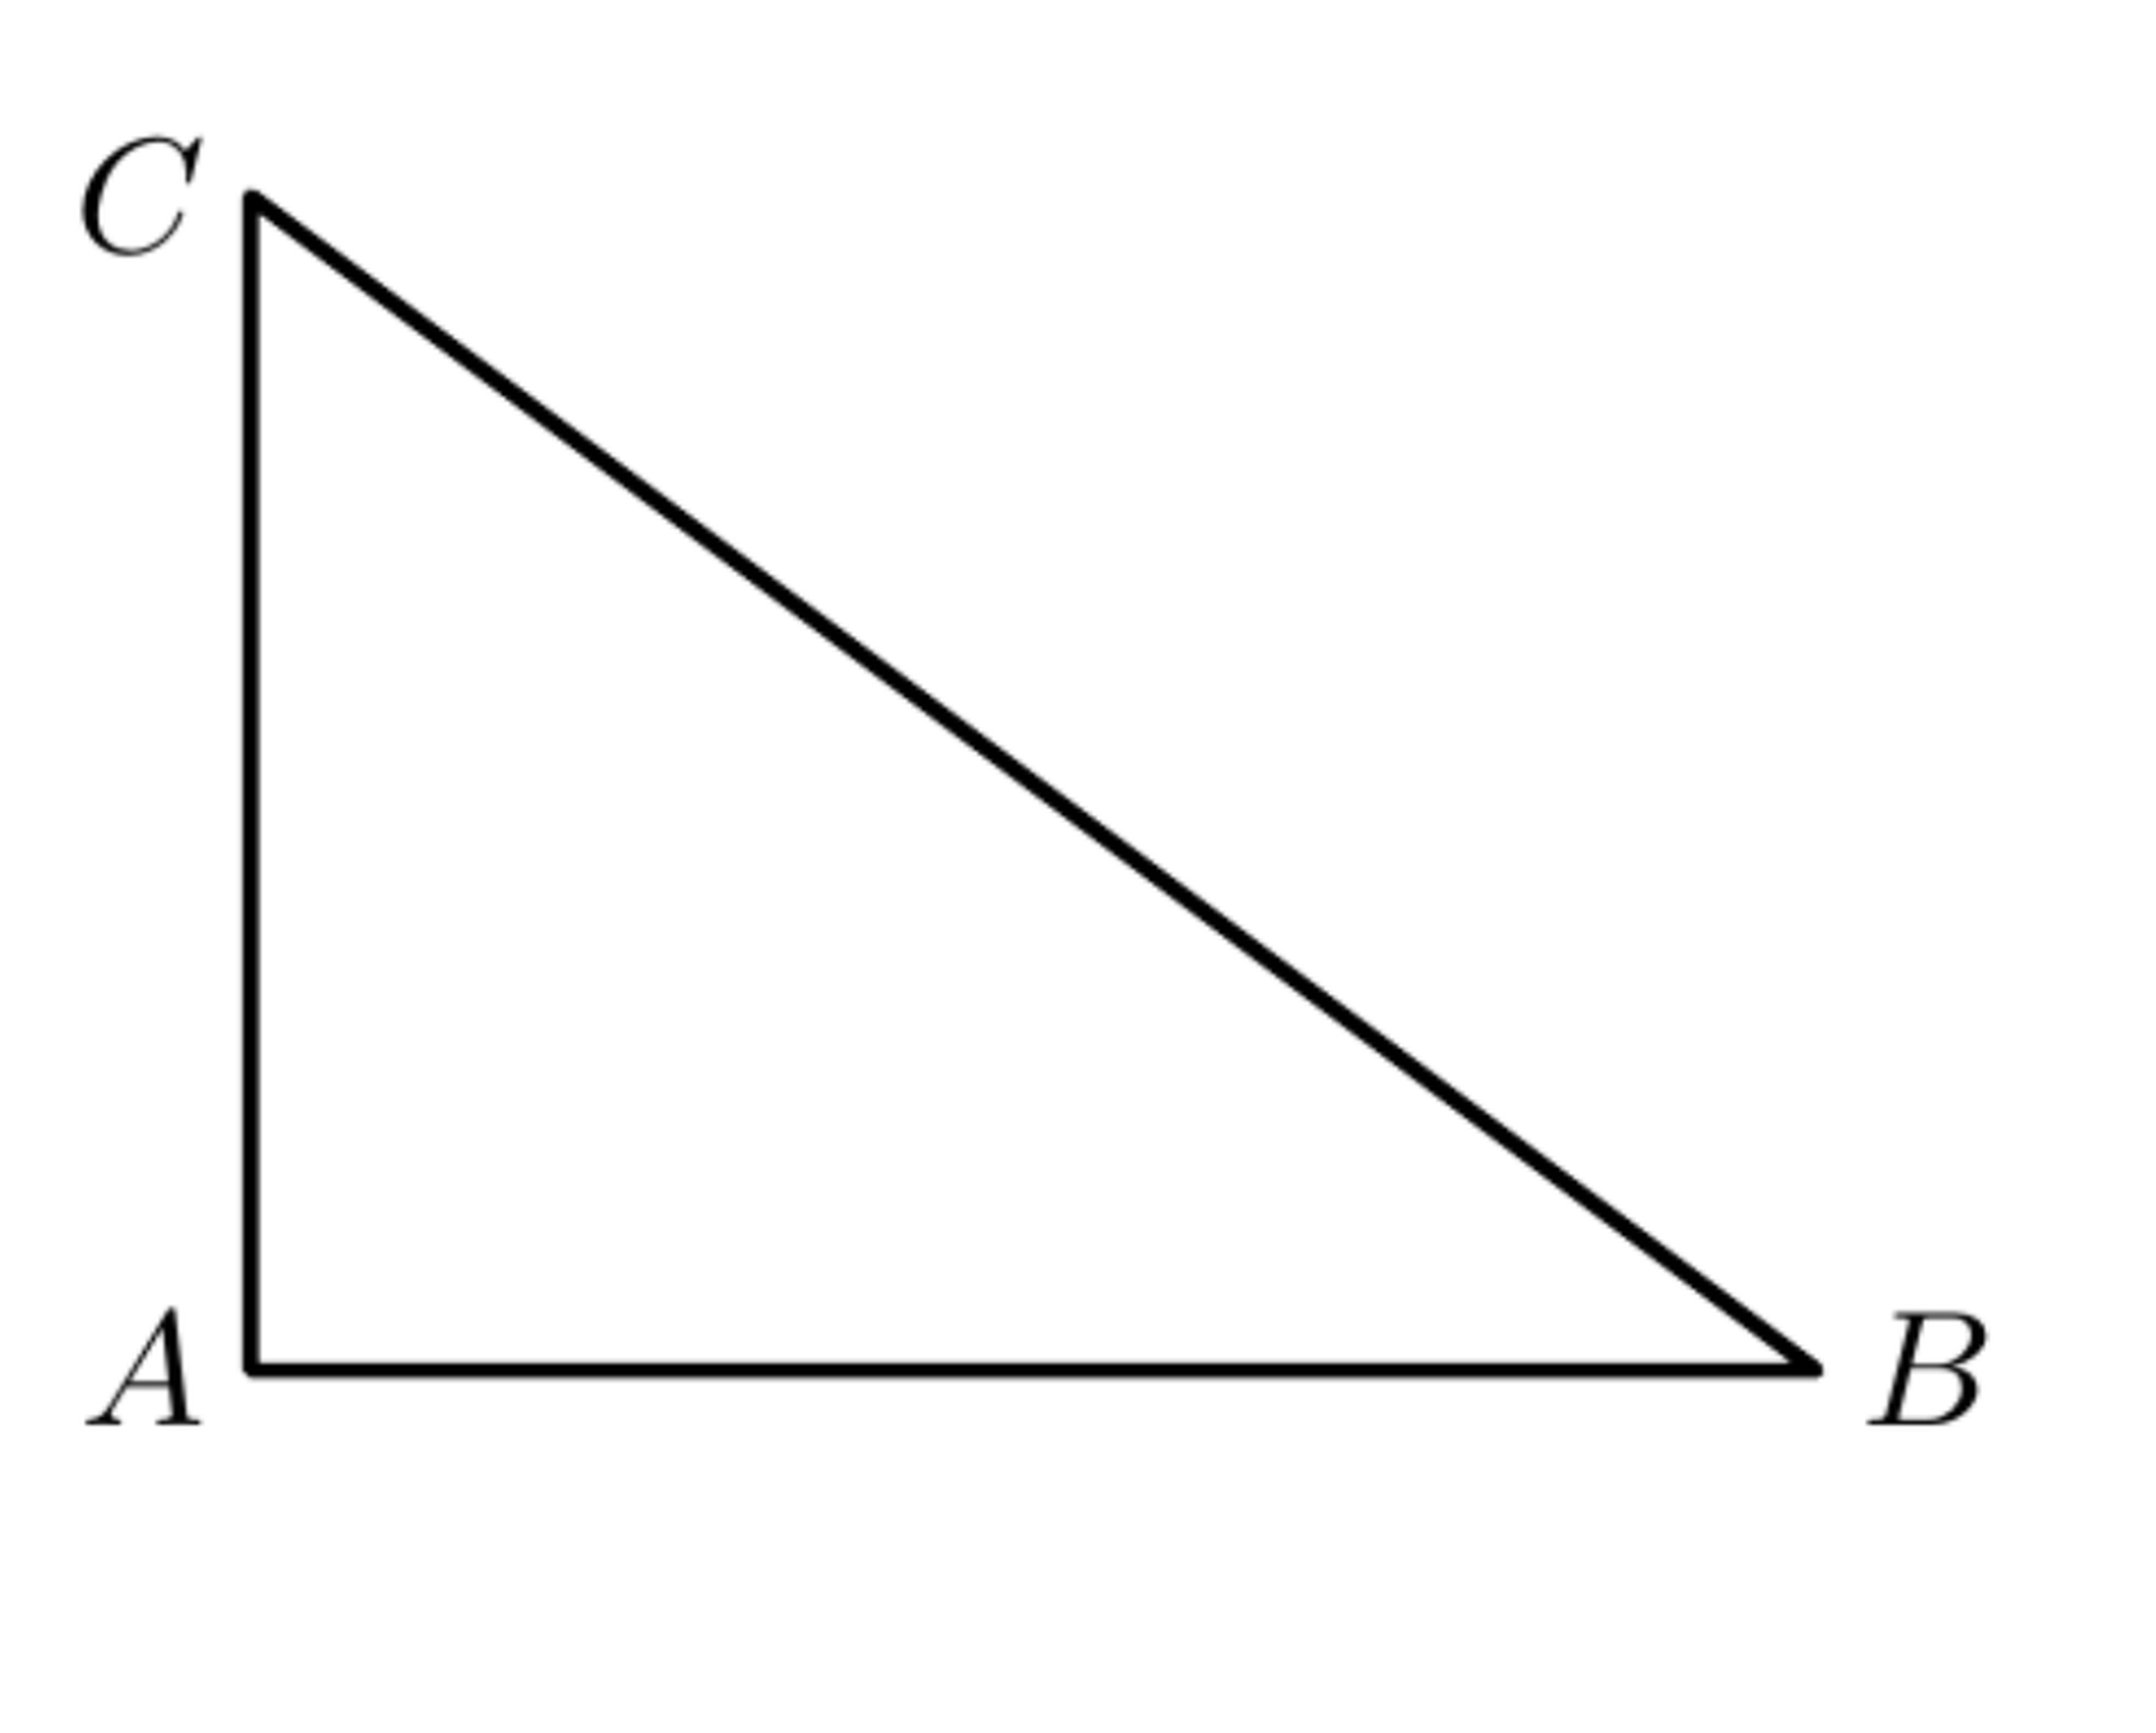
\includegraphics[width=0.34\textwidth]{figures/gao153_q19.png}
\end{center}

\ifanswer
\solbegin
\step{(1) 取 $A(0,0)$、$B(40,0)$、$C(0,30)$，则斜边 $BC$ 所在直线为 $3x+4y=120$.}
\step{正方形落在边界上的两边必分别在两条直角边上.}
\step{设其边长为 $a$m，则对角顶点为 $(a,a)$.}
\step{按题意划出的正方形应尽量大，即对角顶点落在斜边 $BC$ 上，}
\step{因此 $3a+4a=120\Rightarrow a=\dfrac{120}{7}$；}
\step{(2) 斜边长 $BC=\sqrt{30^2+40^2}=50$m，三角形面积为 $600\text{m}^2$.}
\step{设圆的半径为 $r$，圆心到 $AB$、$AC$、$BC$ 的距离分别为 $d_1,d_2,d_3$，}
\step{则三者均不小于 $r$. 连接圆心与三个顶点，}
\step{得 $600=\dfrac12(40d_1+30d_2+50d_3)\geqslant\dfrac12(40+30+50)r=60r$，所以 $r\leqslant10$.}
\step{取三角形的内切圆时等号成立，圆形区域面积的最大值为 $100\pi\text{m}^2$.}
\step{(3) 任取矩形落在绿地边界上的一边，以其所在直线为横轴.}
\step{设相应三角形底边长为 $L$、高为 $H$，则 $LH=1200$.}
\step{取三角形顶点坐标为 $(0,0)$、$(L,0)$、$(p,H)$.}
\step{在高度 $t$ 处，两腰上的点的横坐标分别为 $\dfrac{pt}{H}$、$L+\dfrac{(p-L)t}{H}$，}
\step{因此，高为 $t$ 的矩形，其底边长不超过 $L\left(1-\dfrac tH\right)$，}
\step{面积满足 $S\leqslant Lt\left(1-\dfrac tH\right)=\dfrac LH\left[\dfrac{H^2}{4}-\left(t-\dfrac H2\right)^2\right]\leqslant\dfrac{LH}{4}=300$，}
\step{在原坐标系中，取矩形顶点为 $(0,0)$、$(20,0)$、$(20,15)$、$(0,15)$，}
\step{其中 $3\times20+4\times15=120$，矩形完全位于绿地内，面积为 $300\text{m}^2$，}
\step{达到最大值.}
\solend
\fi

% === Q20 === $g(x)$ 定义照录；解析 14 行
\item 已知 $a>0$ 且 $a\ne1$，设 $f(x)=\log_a(x^2-a^2)$，$g(x)=2\log_a(x-ak)$.

(1) 求函数 $y=f(x)$ 的定义域；

(2) 若 $k=2$，求不等式 $f(x)>g(x)$ 的解集；

(3) 若“存在实数 $x$，使得 $f(x)=g(x)$”为真命题，求实数 $k$ 的取值范围.

\ifanswer
\solbegin
\step{(1) $x^2-a^2>0\Leftrightarrow x<-a$ 或 $x>a$，定义域为 $(-\infty,-a)\cup(a,+\infty)$.}
\step{(2) 两函数均有意义时，$x>2a$，且 $g(x)=\log_a(x-2a)^2$.}
\step{当 $a>1$ 时，$f(x)>g(x)\Leftrightarrow x^2-a^2>(x-2a)^2\Leftrightarrow x>\dfrac{5a}{4}$，}
\step{结合 $x>2a$，解集为 $(2a,+\infty)$.}
\step{当 $0<a<1$ 时，$f(x)>g(x)\Leftrightarrow x^2-a^2<(x-2a)^2\Leftrightarrow x<\dfrac{5a}{4}$，}
\step{与 $x>2a$ 矛盾，解集为 $\varnothing$.}
\step{(3) 在 $x^2-a^2>0$ 且 $x-ak>0$ 的条件下，}
\step{$f(x)=g(x)\Leftrightarrow x^2-a^2=(x-ak)^2\Leftrightarrow2akx=a^2(1+k^2)$，}
\step{当 $k=0$ 时，上式不成立；}
\step{当 $k\ne0$ 时，$x=\dfrac{a(1+k^2)}{2k}$，}
\step{于是 $x-ak=\dfrac{a(1-k^2)}{2k}>0\Leftrightarrow k<-1$ 或 $0<k<1$，}
\step{对上述 $k$，所取的 $x$ 同时满足 $x^2-a^2=(x-ak)^2>0$，}
\step{两函数均有意义且函数值相等.}
\step{因此，$k$ 的取值范围为 $(-\infty,-1)\cup(0,1)$.}
\solend
\fi

% === Q21 === 中文弯引号、复杂式照录；解析 23 行（跨 08→09 页）
\item 若实数 $x$、$y$、$m$ 满足 $\lvert x-m\rvert<\lvert y-m\rvert$，则称 $x$ 比 $y$ 接近 $m$.

(1) 若 $2x$ 比 $x-2$ 更接近 1，求实数 $x$ 的取值范围；

(2) 若 $x$ 比 $y$ 接近 $m$，证明：“$x>y$” 的充要条件是 “$x+y<2m$”；

(3) 已知 $x>0$，$y>0$ 且 $x\ne y$. 设 $p=\dfrac{x^2+y^2}{xy}$，若对于任意的 $x$、$y$，命题 “$p$ 比 $p^2-3p+4$ 接近 $m$” 恒成立，求实数 $m$ 的取值范围.

\ifanswer
\solbegin
\step{(1) $\lvert2x-1\rvert<\lvert x-3\rvert\Leftrightarrow(2x-1)^2<(x-3)^2\Leftrightarrow(x+2)(3x-4)<0$，}
\step{解得 $-2<x<\dfrac43$，实数 $x$ 的取值范围为 $\left(-2,\dfrac43\right)$.}
\step{(2) 因为 $x$ 比 $y$ 接近 $m$，所以 $\lvert x-m\rvert<\lvert y-m\rvert$，则 $\lvert x-m\rvert^2<\lvert y-m\rvert^2$，}
\step{即 $(x-m)^2<(y-m)^2$，即 $(x-m)^2-(y-m)^2<0$，}
\step{即得 $(x-y)(x+y-2m)<0$，}
\step{则由 $x+y<2m$，得 $x+y-2m<0$，}
\step{故 $x-y>0$，即 $x>y$，充分性成立；}
\step{当 $x>y$ 时，$x-y>0$，结合 $(x-y)(x+y-2m)<0$，得 $x+y-2m<0$，}
\step{即 $x+y<2m$，必要性成立；}
\step{故“$x>y$” 的充要条件是 “$x+y<2m$”；}
\step{(3) $x>0$，$y>0$ 且 $x\ne y$. 则 $p=\dfrac{x^2+y^2}{xy}=\dfrac xy+\dfrac yx>2\sqrt{\dfrac xy\cdot\dfrac yx}=2$，}
\step{由于对于任意的 $x$、$y$，命题 “$p$ 比 $p^2-3p+4$ 接近 $m$” 恒成立，}
\step{故 $\lvert p-m\rvert<\lvert(p^2-3p+4)-m\rvert$ 对 $\forall p>2$ 恒成立，}
\step{即得 $(p-m)^2<(p^2-3p+4-m)^2$，}
\step{即 $(p^2-3p+4-m)^2-(p-m)^2>0$，}
\step{得 $(p^2-4p+4)(p^2-2p+4-2m)>0$，}
\step{即 $(p-2)^2(p^2-2p+4-2m)>0$，由于 $p>2$，故 $(p-2)^2>0$，}
\step{故 $p^2-2p+4-2m>0$ 对 $\forall p>2$ 恒成立，}
\step{即 $2m<p^2-2p+4$ 对 $\forall p>2$ 恒成立，}
\step{由于 $p^2-2p+4=(p-1)^2+3$，此时 $p^2-2p+4$ 在 $(2,+\infty)$ 上严格增，}
\step{故 $(p-1)^2+3>(2-1)^2+3=4$，故 $2m\leqslant4$，解得 $m\leqslant2$，}
\step{即实数 $m$ 的取值范围是 $(-\infty,2]$.}
\solend
\fi

\end{enumerate}

\end{document}
"
%
% ① 原始材料：微信公众号"魔都数学加油站"文章，连载"27学年高一153"，原文标题
% "27学年高一153——2026-2027年上海市闵行中学文绮中学高一上期中"；
% 原文链接：https://mp.weixin.qq.com/s/rEtS-92cDR6JKgY2b5DRfg 。
% 正文为 9 张 PNG 页（01/02/06/07/08/09 为 2560×3620，03/04/05 为 4762×6735，
% 同一篇各页分辨率混排，逐页按各自分辨率裁图核对，别按预览比例换算裁框）。
% 体例：讲评版——填空 3—12（10 题）、选择 13—16（4 题）、解答 17—21（5 题），
% 共 19 题，自第 3 题起编；**全 19 题均印【解析】**（逐题核实，见 ② ②）。
% 题目、答案、解析均据原图转录；卷面粉红色水印"魔都数学加油站"及公众号页脚未录入。
% 全卷插图清单（逐页通读 9 页确认）：2 幅，均为题目配图、三版都出——
%   · Q11 正方形 OABC 曲线图（02 页右下：$y=5x^2$ 与 $y=x^{-\frac12}$ 两条曲线、
%     坐标轴、O/A/B/C/P/Q、正方形），裁 figures/gao153_q11.png；
%   · Q19 直角三角形 ABC 绿地示意图（05 页右上，直角在 A），
%     裁 figures/gao153_q19.png；
%   两图均去粉色水印、去色、4× LANCZOS 放大；Q11 图左上角题干残字"函"已裁白。
%   其余各页逐页确认无其它题目配图、无解析内配图、无表格；09 页下半仅水印、无正文。
%
% 卷首标题：原卷印作"2026-2027 年闵行中学文绮中学高一上期中"，年份区间按全稿惯例排 en dash；
% 原卷卷面未印副标题，本稿按同期中卷知识模块口径补出"集合与常用逻辑用语、不等式、函数"。
%
% ② 与原卷的排版差异：
%   ① 原文从第 3 题起，本稿保留原题号；共 19 题三节，解答题 5 题到 21；
%   ② 全 19 题均印【解析】、用 \solbegin…\solend，无只印【答案】或答案印括号内的题；
%      四道选择题答案在解析末句"故选 A／A／D／C"（Q13—Q16，逐个放大复核）、
%      括号 \mbox{（\quad）} 留空、不另提 \ans{}；答案版【答案】/【解析】标记数
%      = 19 = 全卷题数；
%   ③ 原卷卷面未印副标题，本稿按知识模块口径补出；
%   ④ 原卷填空横线按全稿惯例排 \blankline[4.4em]；选择题括号排 \mbox{（\quad）}、
%      四道选择题的选项段前按惯例各加 \keepwithprev；解答题不留作答区、不加
%      \anspace（原卷为讲评版，109—113 起全稿不用 \anspace）；
%   ⑤ 数集：Q3"$x\in R$"、Q5"解集为 R"、Q10"$x\in N$"、Q12"$x\in Z$"与
%      "$m\in Z$"、Q14"$m\in Z$"、Q16"$a\in N$"、Q17"全集 $U=R$"、
%      Q19 无、Q21 无——原卷印斜体或正体粗体 R/N/Z，按全稿惯例归一
%      \R／\N／\Z；绝对值排 \lvert…\rvert（Q5、Q11、Q21），集合描述竖线排 \mid
%      （Q3、Q10、Q17、Q20），不等号按全稿惯例排 \leqslant／\geqslant；
%      补集照原卷上划线排 \overline{A}（Q17 题干 (2)＋解析 (2)）；
%      空集 \varnothing（Q12 题干、Q20 解析 (2)）；子集 3 处均印带下划线 ⊆、
%      照录 \subseteq（Q10 $A\subseteq U$、Q12 $B\subseteq A$、Q17 $(-1,2)\subseteq(a-5,a)$），
%      本卷无单线 \subset 用例；
%   ⑥ 判别式：逐页通读 9 页，本卷无一元二次判别式 Δ/△ 算式，故无 Δ/△ 混用可照录；
%      Q11 图里有几何正方形 OABC（非三角形符号），无 △ABC 用例；
%   ⑦ 中文弯引号照录：Q14"$m=0$"与"幂函数…关于原点成中心对称"、
%      Q20"存在实数 $x$，使得 $f(x)=g(x)$"、Q21"$x>y$"与"$x+y<2m$"、
%      "$p$ 比 $p^2-3p+4$ 接近 $m$"（引号外留空格按原卷）；
%      注释里一律 ASCII 引号；数学式内 CJK 用 \text{}；
%   ⑧ "图像／图象"逐处放大核：全卷 3 处均印"图像"（像，有亻）——
%      Q13 题干与解析、Q14 题干与解析；Q19 题干写"如图所示"（非"图像"），
%      逐处照录未统一；子题标号 (1)(2)(3) 半角括号照录；圈数字本卷无用例；
%   ⑨ 半角逗号在数学组之间是全稿惯例、非笔误，逐处照录（Q3 $x\in R$、
%      Q10 $a_1,a_2$、Q19 $A(0,0)$、$d_1,d_2,d_3$、Q21 $a>\frac13,b>\frac13$ 等）；
%      行末西文句点 ASCII `.`；行中全角逗号／顿号照录（Q19"30m 和 40m"、
%      Q21"实数 $x$、$y$、$m$"）；
%   ⑩ 复杂式照录别简化：Q3 $y=x^{-2}$、Q11 $y=x^{-\frac12}$ 与
%      $\frac{2}{\sqrt[4]{5}}$、Q8 $\frac{2b}{a+1-b}$、Q9 cases 块、
%      Q10 $525=5\times105$、Q16 $a^2+1$、Q19 $S\leqslant Lt(1-\frac tH)$
%      与 $L+\frac{(p-L)t}{H}$、Q20 $2akx=a^2(1+k^2)$ 与 $\frac{a(1+k^2)}{2k}$、
%      Q21 $(p^2-4p+4)(p^2-2p+4-2m)>0$；
%      \left…\right 不得拆到不同 $…$ 组（Q17 $\left\{x\mid\cdots\right\}$、
%      Q19 $\left[\frac{H^2}{4}-\left(t-\frac H2\right)^2\right]$、
%      Q21 $\left(-2,\frac43\right)$ 等）；cases 块一律 \begin{cases}…\end{cases}；
%   ⑪ 一条 \step = 原卷解析的一个印刷行，cases 块整体算一个印刷行；别并折行、
%      别拆行。Q10 六行、Q19 十九行、Q20 十四行、Q21 二十二行均按印刷行逐条断，
%      不丢行；
%   ⑫ 配图：Q11／Q19 题目配图（三版都出）放 \item 内题干之后 \begin{center}，
%      各用 \needvspace{8cm} 守卫把整块推走，**守卫放在 \item 之前**
%      （见 高一145 Q14/Q20 成例与切页审计 B 类坑）；
%   ⑬ 原卷解析内无红色"法一／法二"之类小标题，故本卷无 \stepm；红色水印
%      "魔都数学加油站"不录入；
%   ⑭ 跨页续印按题合并：见 ⑥；
%
% ③ 行数复核：一条 \step = 原卷解析的一个印刷行，cases 块作一个印刷行计。
%   逐题数（主会话逐页核对定稿）：Q3：1；Q4：2；Q5：2；Q6：2；Q7：1；
%   Q8：1；Q9：2；Q10：6；Q11：3；Q12：5；Q13：2；Q14：3；Q15：5；
%   Q16：3；Q17：5；Q18：4；Q19：19；Q20：14；Q21：22。
%   合计 102 条 \step（本卷无 \stepm），与原卷逐题印刷行相等。全卷 19 题
%   均设 \solbegin…\solend，答案版【答案】/【解析】标记数 = 19 = 全卷题数。
%
% ④ 判别式／子集符号结论（逐处放大原图照录、不得统一，主会话像素级复核）：
%   判别式：逐页通读 9 页，本卷无一元二次判别式算式（Q7 用韦达定理、
%      Q16 用因式分解、Q20 用对数方程，均不写 Δ/△），故无 Δ/△ 混用可照录
%      （"高 \Delta／扁 \triangle"口径备查，参照 高一142／151／152 头注）；
%      本卷无几何三角形符号用例。
%   子集：Q10 题干"$A\subseteq U$"、Q12 题干"$B\subseteq A$"、Q17 解析 (2)
%      "$(-1,2)\subseteq(a-5,a)$"共 3 处，逐处放大确认均印带下划线 ⊆、
%      照录 \subseteq；本卷未见单线 ⊂（\subset）之对应处。
%      补集上划线 \overline{A}（Q17）、空集 \varnothing（Q12 题干、Q20 解析 (2)）；
%      数集 \R／\N／\Z 归一见 ② ⑤。
%
% ⑤ 存疑照录（放大原图确认，照录未改、正文对应处另有 % 注）：
%   1. Q3 集合 $B=\{(x,y)\mid y=x^{-2},x\in\R\}$ 原卷题干径写 $x\in\R$
%      （$x=0$ 处无意义），解析自行注明 $x\ne0$，照录未改。
%   2. Q10 解析"$U$ 中共有 $525=5\times105$ 个连续整数"与尾行
%      "取 $U$ 中除以 5 余 1 或 2 的全部元素及元素 5"逐字照录（放大 02 页
%      /tmp/gao153/z/zoom/q10_pick.png 确认是"元素 5"，非"元素 9"）。
%   3. Q11 第二个函数原卷印 $y=x^{-\frac12}$（负二分之一次幂，非 $x^2$），
%      放大 02 页 /tmp/gao153/z/zoom/q11_exp.png 确认，照录未改；
%      $|AQ|=\frac1{\sqrt a}$ 与之自洽。
%   4. Q19 (3) 解析"在高度 $t$ 处，两腰上的点的横坐标分别为 $\frac{pt}{H}$、
%      $L+\frac{(p-L)t}{H}$"，放大 06 页确认，照录未简化。
%   5. Q20 (2) 解析"$g(x)=\log_a(x-2a)^2$"（真数整体平方），
%      与 $g(x)=2\log_a(x-ak)$ 在 $k=2$ 时一致，照录未改。
%   6. Q21 (3) 解析"得 $(p^2-4p+4)(p^2-2p+4-2m)>0$"与
%      "故 $(p-1)^2+3>(2-1)^2+3=4$，故 $2m\leqslant4$"照录未改
%      （放大 09 页 /tmp/gao153/z/zoom/q21_factor.png 确认）。
%   7. "图像／图象"全卷 3 处均印"图像"（像，有亻）逐处照录；
%      本卷无判别式 Δ/△ 用例（见 ④）。
%   全卷除此 7 类外未发现其它笔误／自相矛盾处；19 题均印【解析】、
%   无只印【答案】或答案印括号内的题（见 ② ②）。
%
% ⑥ 跨页续印按题合并说明（逐页核实定稿）：Q3—Q5 题干＋解析在 01 页；
%   Q6—Q8 题干＋解析在 01 页下半（Q8 解析续 02 页顶）；Q9 题干＋解析、
%   Q10 题干＋解析首 2 行在 02 页上半，Q10 解析余 4 行在 02 页下半；
%   Q11 题干＋配图＋解析、Q12 题干＋解析 5 行在 02 页下半—03 页上半；
%   "二、选择题"标题在 03 页中部；Q13 题干＋选项＋解析在 03 页下半；
%   Q14 题干＋选项＋解析、Q15 题干＋选项＋解析首行在 03 页下半—04 页顶；
%   Q15 解析余 4 行、Q16 题干＋选项＋解析在 04 页上半；"三、解答题"
%   标题在 04 页下半；Q17 题干＋两问＋解析 5 行在 04 页下半—05 页顶；
%   Q18 题干＋两问＋解析 4 行、Q19 题干（含配图）＋三问在 05 页；
%   Q19 解析 (1)(2) 9 行在 05 页下半，解析 (3) 前 5 行在 06 页上半、
%   余 4 行在 06 页下半；Q20 题干＋三问在 06 页下半，解析 (1)(2)(3)
%   前 6 行在 07 页上半、(3) 余 8 行在 07 页下半；Q21 题干＋三问在
%   07 页末，解析 (1)(2) 10 行在 08 页上半—下半，解析 (3) 前 4 行在
%   08 页下半、余 9 行续 09 页上半，末行"即实数 $m$ 的取值范围是
%   $(-\infty,2]$"为全卷收尾（09 页下半仅水印、无正文）。
%   本稿按题连排，不丢行、不并折行；全卷末题为第 21 题，无附加题节。
%
\documentclass[a4paper,11pt]{article}
\usepackage{common}

\begin{document}

\examtitlest[3]{2026--2027 年闵行中学文绮中学高一上期中}{集合与常用逻辑用语、不等式、函数}

\bigsec{一、填空题}

\begin{enumerate}
\setcounter{enumi}{2}

% === Q3 === 集合描述竖线 \mid；$y=x^{-2}$ 照录；解析 1 行
\item 已知 $A=\{(x,y)\mid y=x^3,x\in\R\}$，$B=\{(x,y)\mid y=x^{-2},x\in\R\}$，则 $A\cap B=$\blankline[4.4em].

\ifanswer
\solbegin
\step{$x^3=x^{-2}\ (x\ne0)\Leftrightarrow x^5=1\Leftrightarrow x=1$，此时 $y=1$，所以 $A\cap B=\{(1,1)\}$.}
\solend
\fi

% === Q4 === 解析 2 行
\item 若关于 $x$ 的不等式 $\dfrac{x-a}{x+1}>0$ 的解集为 $(-\infty,-1)\cup(4,+\infty)$，则实数 $a=$\blankline[4.4em].

\ifanswer
\solbegin
\step{关于 $x$ 的不等式 $\dfrac{x-a}{x+1}>0$ 即 $(x+1)(x-a)>0$.}
\step{再由它的解集为 $(-\infty,-1)\cup(4,+\infty)$，得 $-1$ 和 4 是 $(x+1)(x-a)=0$ 的两个实数根，故 $a=4$.}
\solend
\fi

% === Q5 === 绝对值 \lvert…\rvert；解析 2 行
\item 若关于 $x$ 的不等式 $\lvert x+1\rvert+\lvert x-2\rvert>m$ 的解集为 $\R$，则实数 $m$ 的取值范围是\blankline[4.4em].

\ifanswer
\solbegin
\step{$\lvert x+1\rvert+\lvert x-2\rvert\geqslant\lvert(x+1)-(x-2)\rvert=3$，当且仅当 $-1\leqslant x\leqslant2$ 时取等号，}
\step{因此 $m<3$.}
\solend
\fi

% === Q6 === 解析 2 行
\item 已知指数函数 $y=a^x$（$a>1$）在区间 $[-1,1]$ 上的最大值比最小值大 $\dfrac32$，则实数 $a=$\blankline[4.4em].

\ifanswer
\solbegin
\step{$a>1$，指数函数在 $[-1,1]$ 上严格增，故 $a-\dfrac1a=\dfrac32\Leftrightarrow(a-2)(2a+1)=0$.}
\step{结合 $a>1$，得 $a=2$.}
\solend
\fi

% === Q7 === 韦达定理；解析 1 行
\item 已知关于 $x$ 的一元二次方程 $x^2+px+2p=0$ 的两个实数根分别为 $x_1$、$x_2$，且 $(x_1+1)(x_2+1)=0$，则 $p=$\blankline[4.4em].

\ifanswer
\solbegin
\step{$0=(x_1+1)(x_2+1)=x_1x_2+x_1+x_2+1=2p-p+1=p+1\Rightarrow p=-1$.}
\solend
\fi

% === Q8 === 换底公式；解析 1 行
\item 已知 $10^a=3$，$\lg5=b$，则 $\log_6 25=$\blankline[4.4em]（用关于 $a,b$ 的关系式表示）.

\ifanswer
\solbegin
\step{$\lg3=a$，$\lg2=1-b$，所以 $\log_6 25=\dfrac{\lg25}{\lg6}=\dfrac{2b}{a+1-b}$.}
\solend
\fi

% === Q9 === cases 块整体算一个印刷行；解析 2 行
\item 已知 $A=[2,5]$，若对任意 $x\in A$，总有 $\dfrac{k}{x}\in A$，则正数 $k=$\blankline[4.4em].

\ifanswer
\solbegin
\step{$k>0$，当 $x\in[2,5]$ 时，$\dfrac{k}{x}$ 的取值范围为 $\left[\dfrac k5,\dfrac k2\right]$，}
\step{因此 $\begin{cases}\dfrac k5\geqslant2\\\dfrac k2\leqslant5\end{cases}\Leftrightarrow10\leqslant k\leqslant10\Leftrightarrow k=10$.}
\solend
\fi

% === Q10 === $A\subseteq U$ 带下划线照录；解析 6 行
\item 已知集合 $U=\{x\mid4\leqslant x\leqslant528,x\in\N\}$，$A=\{a_1,a_2,a_3,\cdots,a_n\}$，且 $A\subseteq U$. 如果集合 $A$ 中的任意两个不同元素之和都不能被 5 整除，则正整数 $n$ 的最大值为\blankline[4.4em].

\ifanswer
\solbegin
\step{$U$ 中共有 $525=5\times105$ 个连续整数，按除以 5 的余数分成五类，}
\step{每类均有 105 个元素.}
\step{余数为 1,4 的两类不能同时选取，余数为 2,3 的两类也不能同时选取，}
\step{余数为 0 的一类最多选 1 个，因此 $n\leqslant105+105+1=211$.}
\step{取 $U$ 中除以 5 余 1 或 2 的全部元素及元素 5，}% 放大 02 页确认是「元素 5」（非 9），照录未改（见 ⑤ 2）
\step{任意两个不同元素之和均不能被 5 整除，此时 $n=211$，最大值为 211.}
\solend
\fi

% === Q11 === 题目配图（三版都出）；\needvspace 守卫放 \item 之前；$y=x^{-\frac12}$ 照录；解析 3 行
\needvspace{8cm}
\item 如图，已知正方形 $OABC$，其中 $OA=a$（$a>1$），函数 $y=5x^2$ 交 $BC$ 于点 $P$，函数 $y=x^{-\frac12}$ 交 $AB$ 于点 $Q$，当 $\lvert AQ\rvert+\lvert CP\rvert$ 最小时，$a$ 的值为\blankline[4.4em].

\begin{center}
% 正方形 OABC 与两条曲线图取 02 页右下，去粉色水印、去色、4× LANCZOS 放大；三版都出
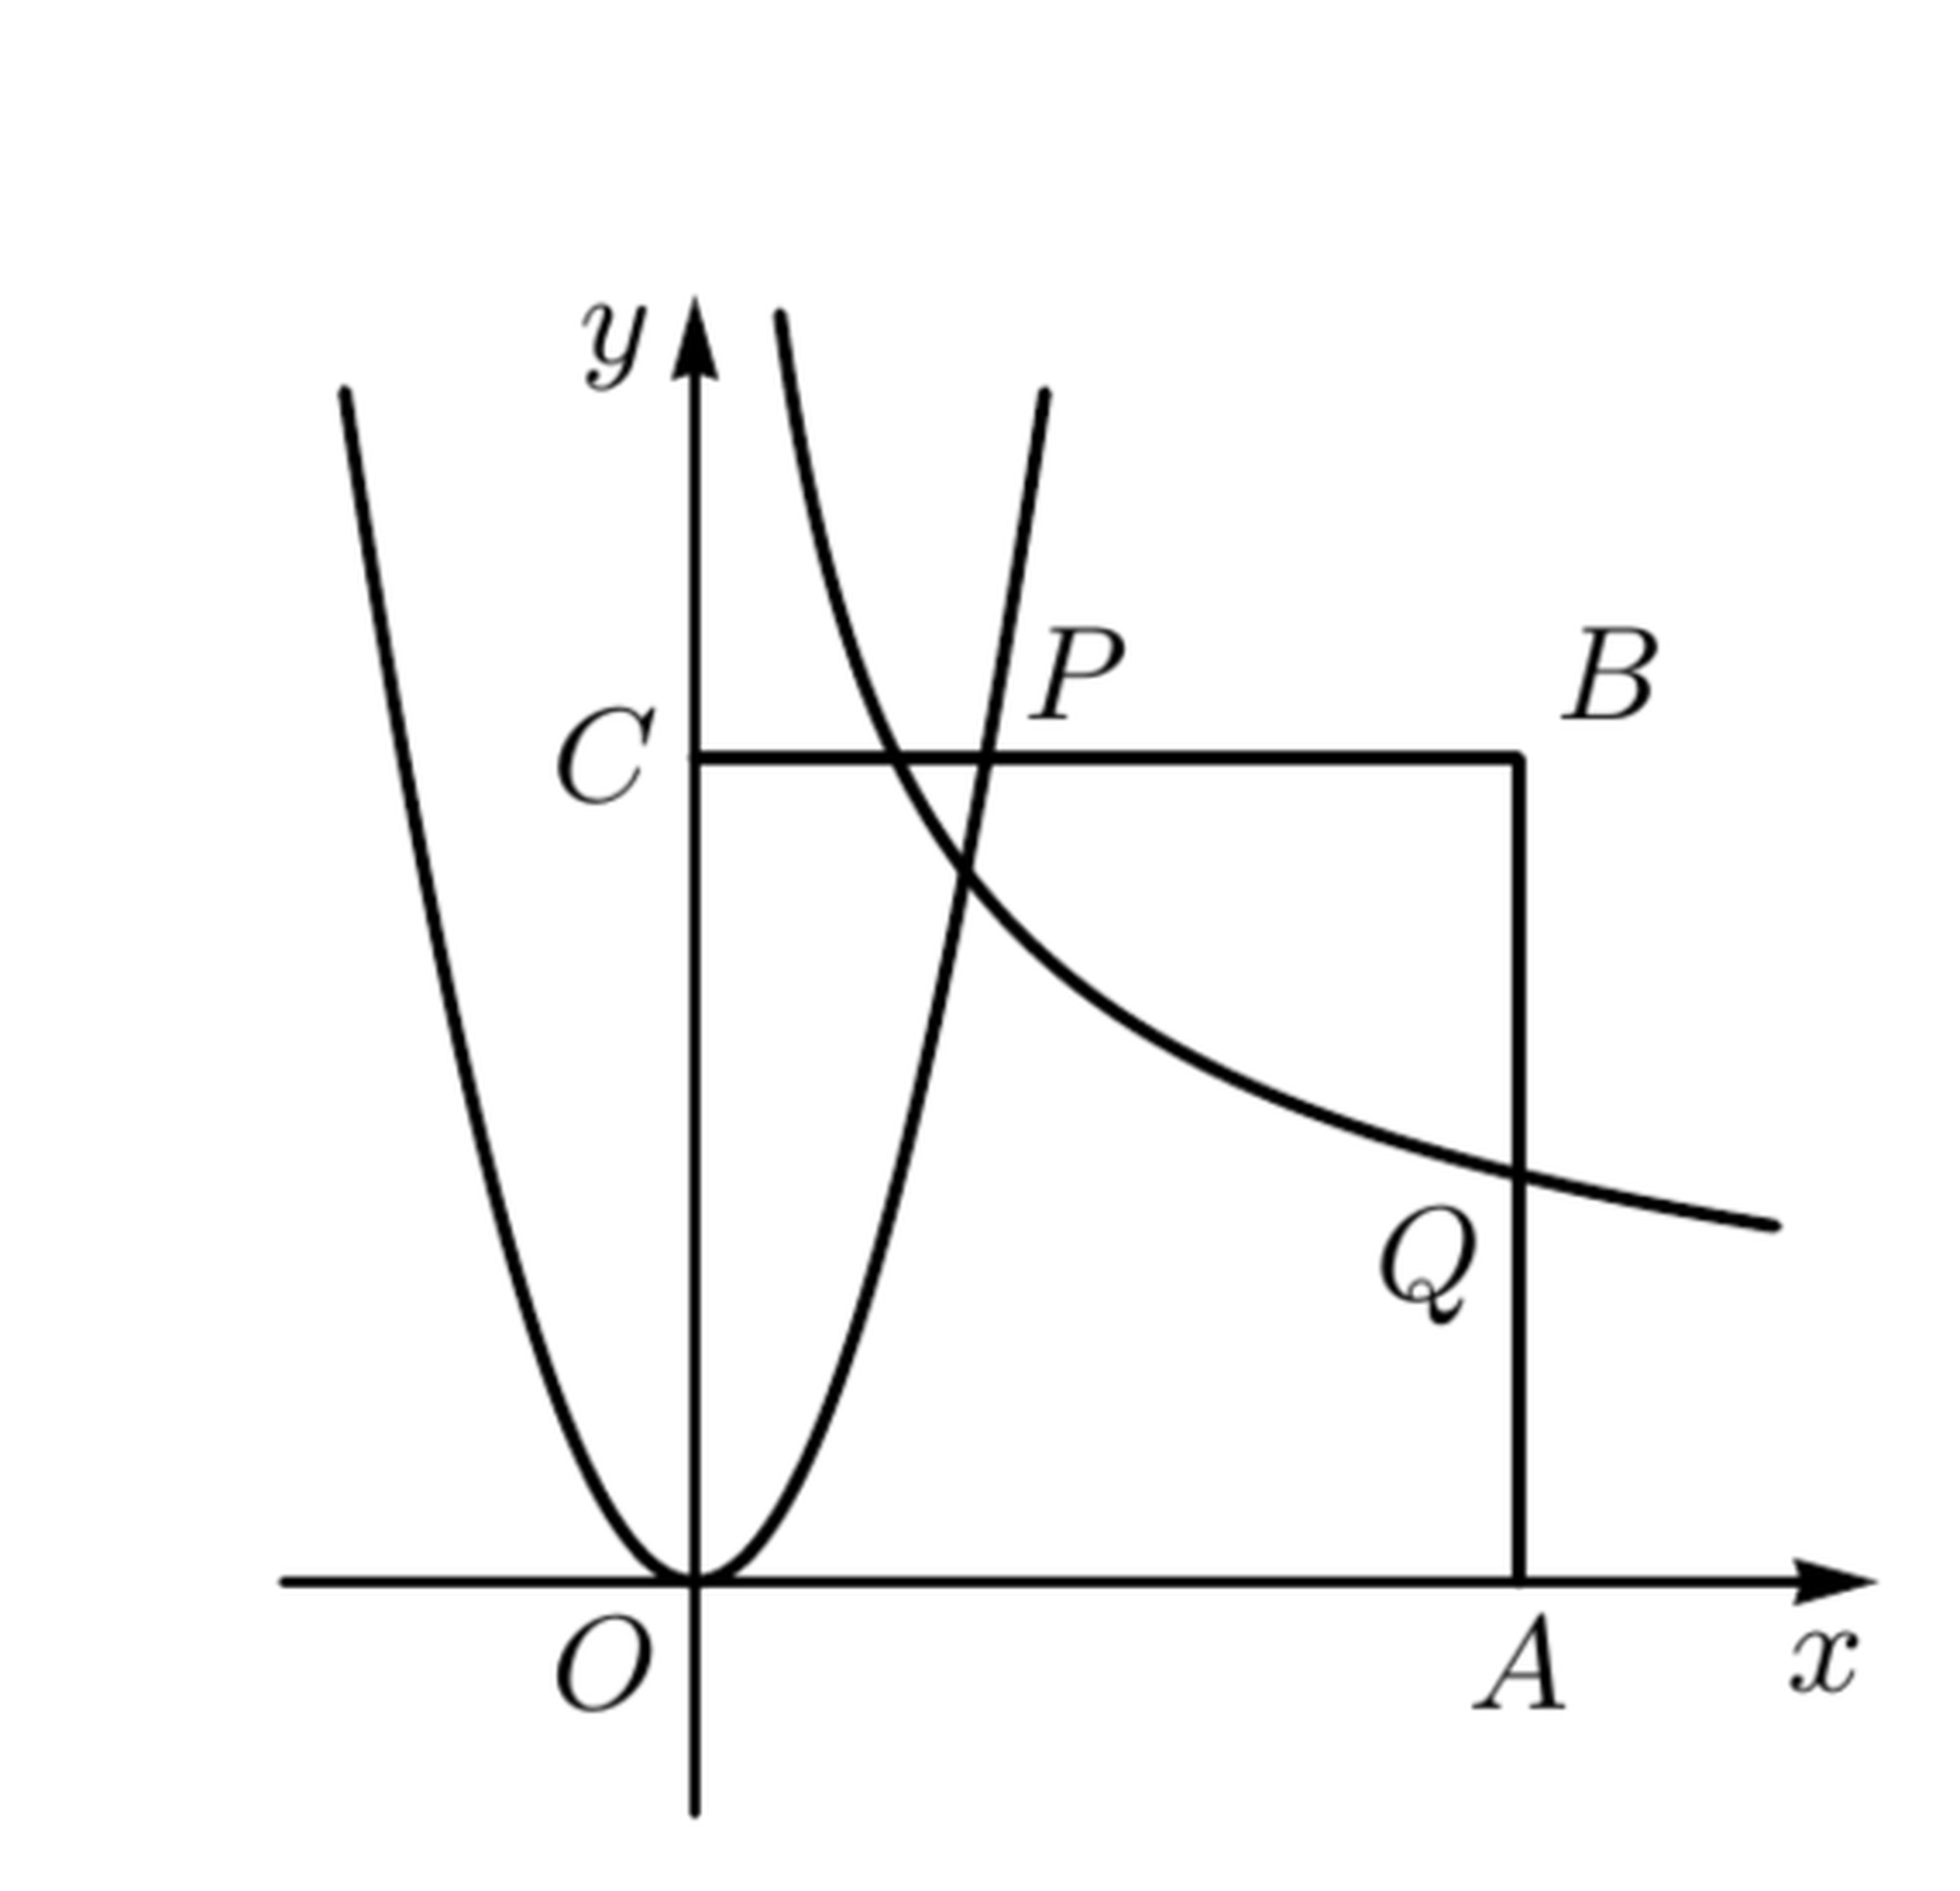
\includegraphics[width=0.40\textwidth]{figures/gao153_q11.png}
\end{center}

\ifanswer
\solbegin
\step{$\lvert AQ\rvert=\dfrac1{\sqrt a}$，$\lvert CP\rvert=\sqrt{\dfrac a5}$，}
\step{于是 $\lvert AQ\rvert+\lvert CP\rvert=\dfrac1{\sqrt a}+\sqrt{\dfrac a5}\geqslant2\sqrt{\dfrac1{\sqrt a}\cdot\sqrt{\dfrac a5}}=\dfrac2{\sqrt[4]{5}}$，}
\step{当且仅当 $\dfrac1{\sqrt a}=\sqrt{\dfrac a5}$，即 $a=\sqrt5$ 时取等号.}
\solend
\fi

% === Q12 === $B\subseteq A$ 带下划线照录、空集 \varnothing；解析 5 行
\item 若集合 $A=\{x\mid1\leqslant x\leqslant100,x\in\Z\}$，集合 $B\subseteq A$，且 $B\ne\varnothing$，记 $W(B)$ 为 $B$ 中元素的最大值与最小值之和，则对所有的 $B$，$W(B)$ 的平均值是\blankline[4.4em].

\ifanswer
\solbegin
\step{对每个非空子集 $B$，令 $B'=\{101-x\mid x\in B\}$，}
\step{则 $W(B')=(101-\min B)+(101-\max B)=202-W(B)$.}
\step{对 $B'$ 再作同样变换即得到 $B$，因此 $B$ 遍历所有非空子集时，}
\step{$B'$ 也恰好遍历所有非空子集.}
\step{设所求平均值为 $m$，则 $m=202-m$，解得 $m=101$.}
\solend
\fi

\end{enumerate}

\bigsec{二、选择题}

\begin{enumerate}
\setcounter{enumi}{12}

% === Q13 === "图像"（像，有亻）照录；解析 2 行，故选 A
\item 设 $a$、$b$ 为常数，若 $0<a<1$，$b>1$，则函数 $y=a^x-b$ 的图像必定不经过\mbox{（\quad）}

\keepwithprev
A. 第一象限\qquad\qquad B. 第二象限\qquad\qquad C. 第三象限\qquad\qquad D. 第四象限

\ifanswer
\solbegin
\step{当 $x>0$ 时，$a^x<1<b$，所以 $y=a^x-b<0$，图像必定不经过第一象限，}
\step{故选 $A$.}
\solend
\fi

% === Q14 === $m\in\Z$、中文弯引号、"图像"照录；解析 3 行，故选 A
\item 已知 $m\in\Z$，则“$m=0$”是“幂函数 $y=x^{m^2-2m-1}$ 的图像与 $x$ 轴及 $y$ 轴均无交点，且关于原点成中心对称”的\mbox{（\quad）}

\keepwithprev
A. 充分不必要条件\qquad\qquad B. 必要不充分条件

C. 充要条件\qquad\qquad D. 既不充分也不必要条件

\ifanswer
\solbegin
\step{图像满足所述条件 $\Leftrightarrow m^2-2m-1$ 为负奇数 $\Leftrightarrow m=0$ 或 $m=2$.}
\step{$m=0$ 能推出所述条件，但所述条件不能推出 $m=0$，因此是充分不必要条件，}
\step{故选 $A$.}
\solend
\fi

% === Q15 === 四选项一行；解析 5 行（跨 03→04 页），故选 D
\item 设 $a>b>1$，$x>1$，则下列不等式正确的是\mbox{（\quad）}

\keepwithprev
A. $a^x<b^x$\qquad B. $x^a<x^b$\qquad C. $\log_a x>\log_b x$\qquad D. $\log_x a>\log_x b$

\ifanswer
\solbegin
\step{$x>1$，幂函数与指数函数的单调性给出 $a^x>b^x$，$x^a>x^b$，A、B 错误.}
\step{$\log_a x=\dfrac{\lg x}{\lg a}<\dfrac{\lg x}{\lg b}=\log_b x$，C 错误.}
\step{对数函数 $y=\log_x t$ 的底数 $x>1$，在 $(0,+\infty)$ 上严格递增，}
\step{所以 $\log_x a>\log_x b$，D 正确.}
\step{故选 $D$.}
\solend
\fi

% === Q16 === $a\in\N$；解析 3 行，故选 C
\item 设 $a\in\N$，则满足不等式 $x^2-a^2x-a^2-1<0$ 的整数 $x$ 的个数不可能是\mbox{（\quad）}

\keepwithprev
A. 1\qquad\qquad B. 50\qquad\qquad C. 100\qquad\qquad D. 2026

\ifanswer
\solbegin
\step{$(x+1)(x-a^2-1)<0\Leftrightarrow-1<x<a^2+1$. 整数解为 $0,1,\cdots,a^2$，共 $a^2+1$ 个.}
\step{$1=0^2+1$，$50=7^2+1$，$2026=45^2+1$，而 $100-1=99$ 不是完全平方数，}
\step{故选 $C$.}
\solend
\fi

\end{enumerate}

\bigsec{三、解答题}

\begin{enumerate}
\setcounter{enumi}{16}

% === Q17 === 补集上划线 \overline{A}、\subseteq 照录；解析 5 行
\item 已知全集 $U=\R$，集合 $A=\{x\mid x^2-x-2\geqslant0\}$，$B=\{x\mid x>-1\}$，$C=\{x\mid a-5<x<a\}$.

(1) 求 $A\cap B$、$A\cup B$；

(2) 若 $\overline{A}\cup C=C$，求实数 $a$ 的取值范围.

\ifanswer
\solbegin
\step{(1) $x^2-x-2=(x+1)(x-2)\geqslant0\Leftrightarrow x\leqslant-1$ 或 $x\geqslant2$，}
\step{所以 $A=(-\infty,-1]\cup[2,+\infty)$，$B=(-1,+\infty)$，}
\step{因此 $A\cap B=[2,+\infty)$，$A\cup B=\R$.}
\step{(2) $\overline{A}=(-1,2)$，于是 $\overline{A}\cup C=C\Leftrightarrow\overline{A}\subseteq C\Leftrightarrow(-1,2)\subseteq(a-5,a)$，}
\step{两区间均为开区间，端点可重合，故 $\begin{cases}a-5\leqslant-1\\a\geqslant2\end{cases}\Leftrightarrow2\leqslant a\leqslant4$.}
\solend
\fi

% === Q18 === 解析 4 行
\item 已知 $a$、$b$、$c$ 都是正数，

(1) 若 $a+b=1$，求证：$\dfrac1a+\dfrac1b\geqslant4$，并指出等号成立的条件；

(2) 若 $a+b+c=1$，求证：三个数 $\dfrac1a$、$\dfrac1b$、$\dfrac1c$ 中至少有一个不小于 3.

\ifanswer
\solbegin
\step{(1) 由 $(a-b)^2\geqslant0$，得 $4ab\leqslant(a+b)^2=1$，所以 $\dfrac1a+\dfrac1b=\dfrac{a+b}{ab}=\dfrac1{ab}\geqslant4$，}
\step{等号成立当且仅当 $a=b$，结合 $a+b=1$，得 $a=b=\dfrac12$.}
\step{(2) 假设三个数 $\dfrac1a$、$\dfrac1b$、$\dfrac1c$ 都小于 3，则 $a>\dfrac13,b>\dfrac13,c>\dfrac13\Rightarrow a+b+c>1$，}
\step{与 $a+b+c=1$ 矛盾，因此三个数中至少有一个不小于 3.}
\solend
\fi

% === Q19 === 题目配图（三版都出）；\needvspace 守卫放 \item 之前；解析 19 行
\needvspace{8cm}
\item 某新建居民小区有一直角三角形绿地，两直角边长分别为 30m 和 40m，打算在其中划出一片区域改造成活动场地，如图所示.

(1) 若划出的区域为正方形，且有两边落在绿地边界上，求此正方形边长；

(2) 若划出的区域为圆形，求圆形区域面积的最大值；

(3) 若划出的区域为矩形（其中至少有一边在边界上），求此矩形面积的最大值.

\begin{center}
% 直角三角形 ABC 绿地示意图取 05 页右上，去粉色水印、去色、4× LANCZOS 放大；三版都出
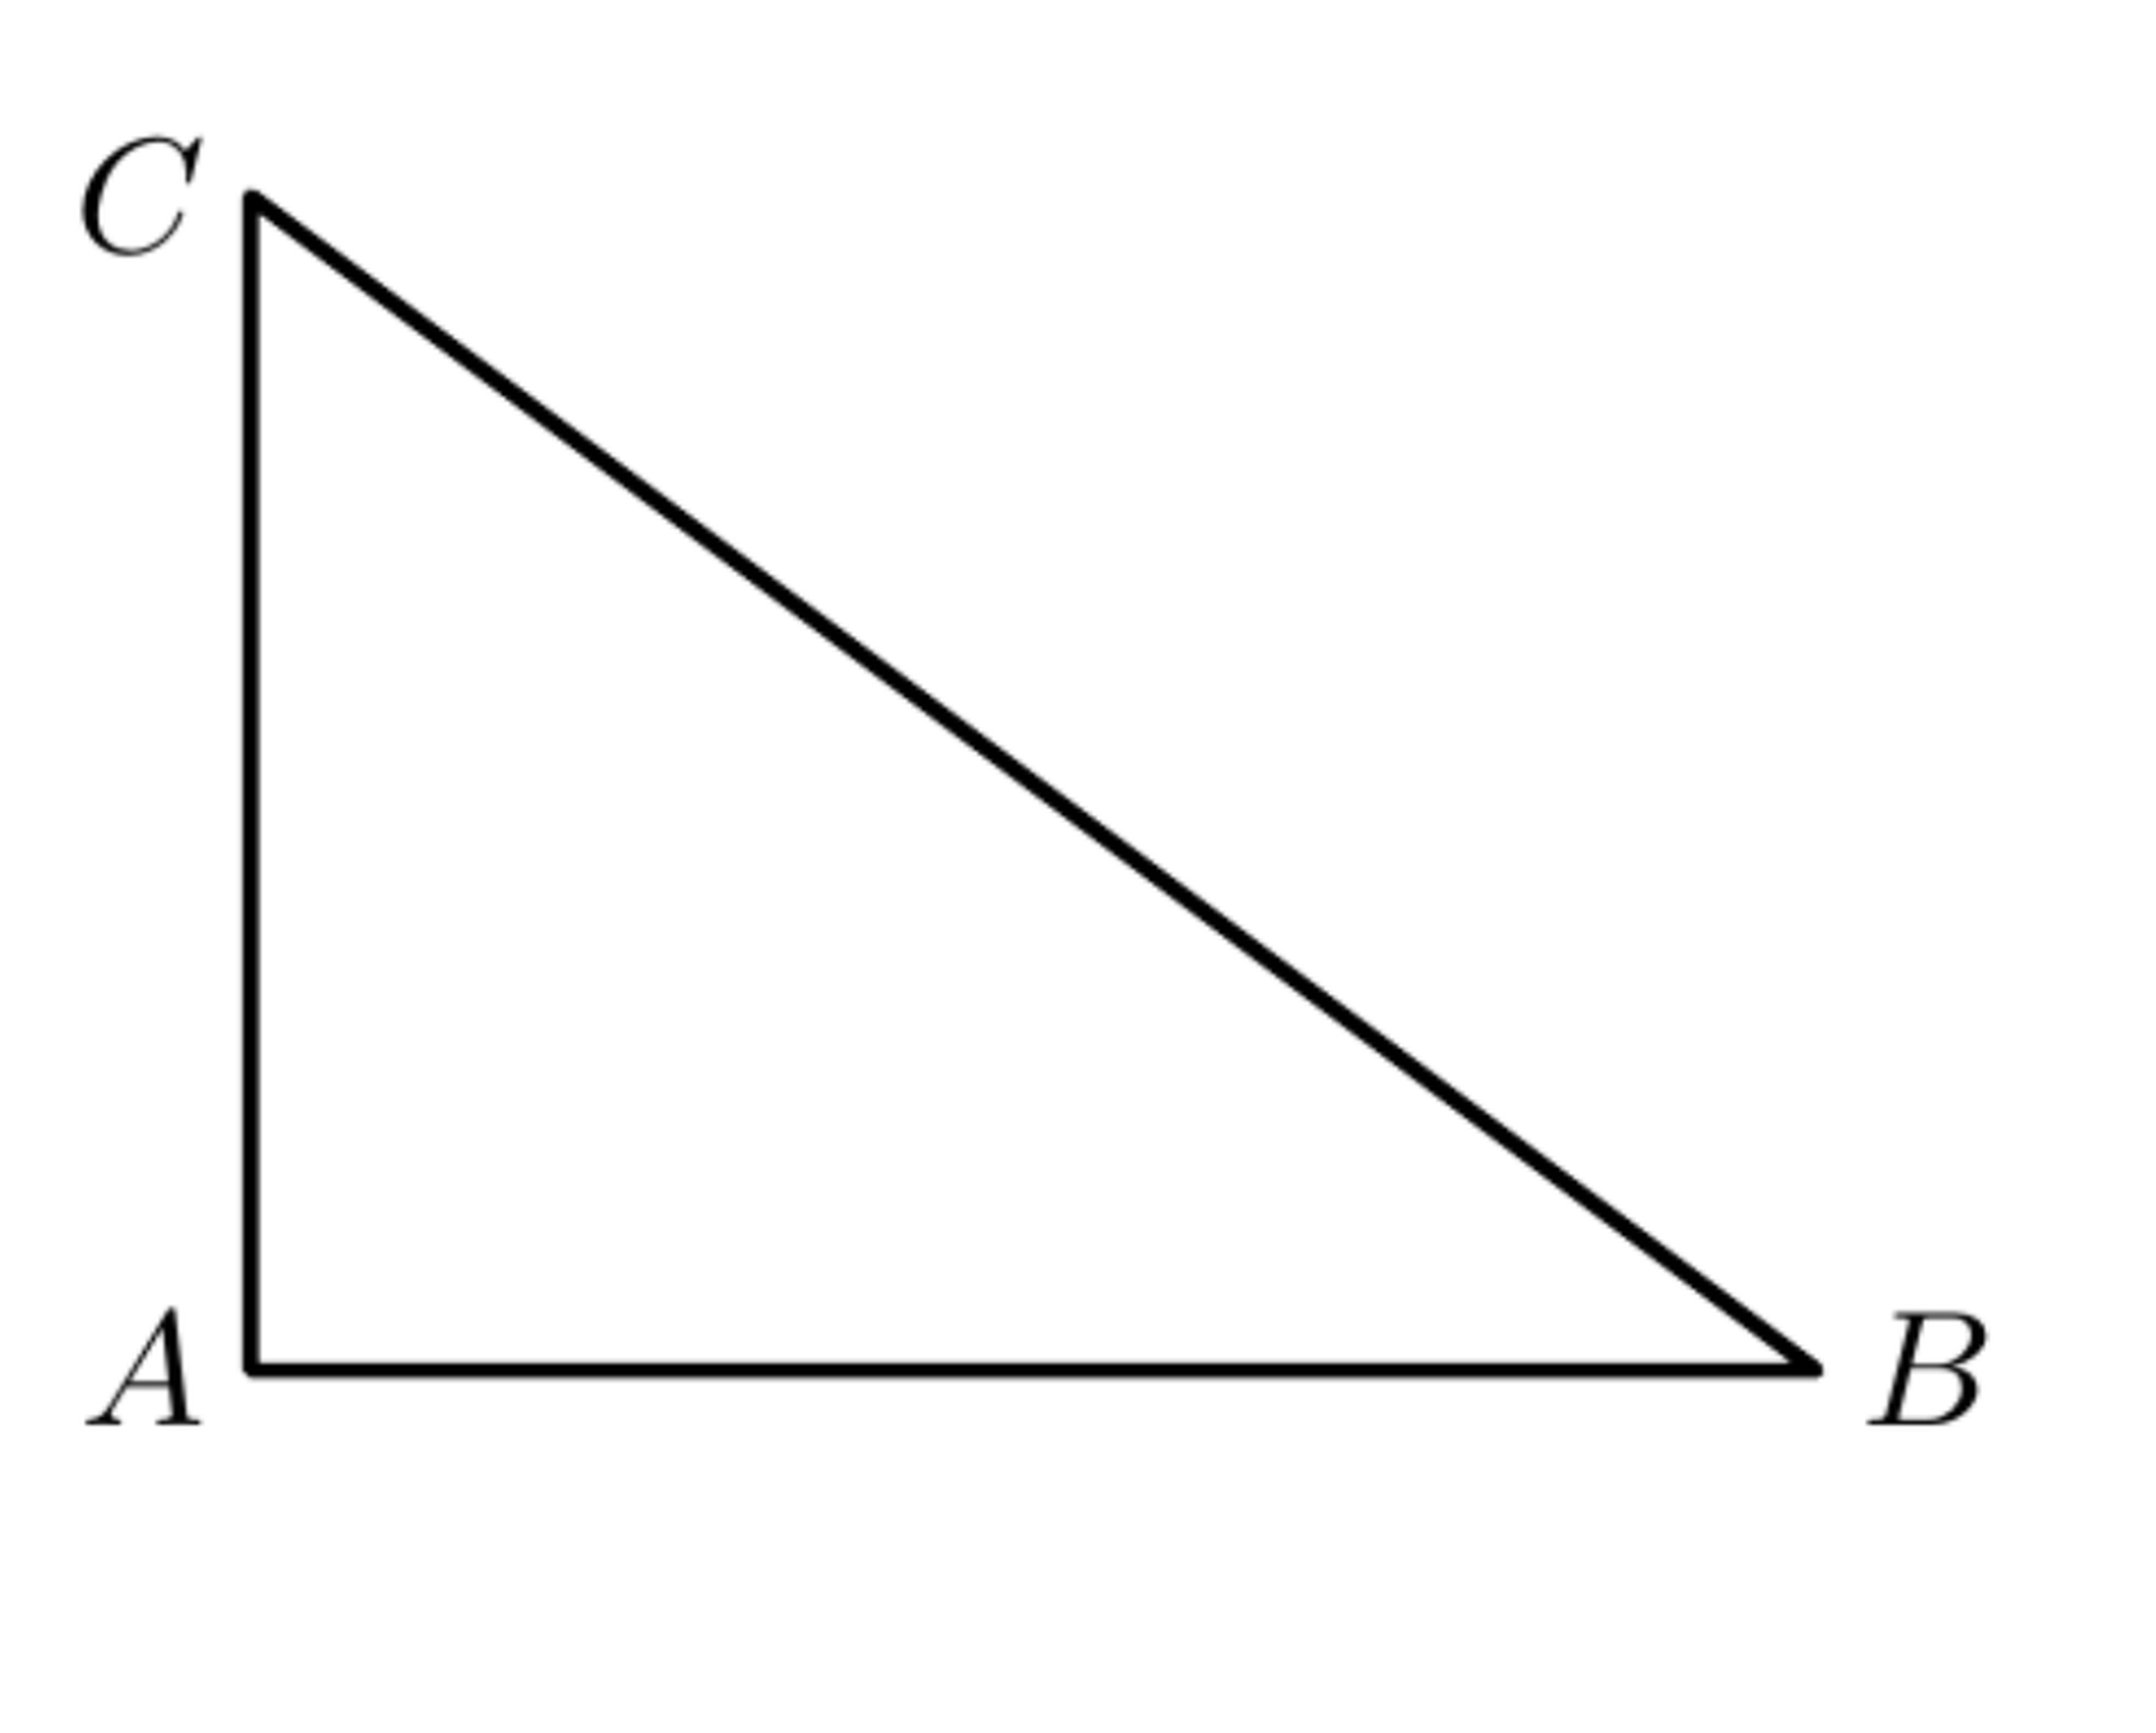
\includegraphics[width=0.34\textwidth]{figures/gao153_q19.png}
\end{center}

\ifanswer
\solbegin
\step{(1) 取 $A(0,0)$、$B(40,0)$、$C(0,30)$，则斜边 $BC$ 所在直线为 $3x+4y=120$.}
\step{正方形落在边界上的两边必分别在两条直角边上.}
\step{设其边长为 $a$m，则对角顶点为 $(a,a)$.}
\step{按题意划出的正方形应尽量大，即对角顶点落在斜边 $BC$ 上，}
\step{因此 $3a+4a=120\Rightarrow a=\dfrac{120}{7}$；}
\step{(2) 斜边长 $BC=\sqrt{30^2+40^2}=50$m，三角形面积为 $600\text{m}^2$.}
\step{设圆的半径为 $r$，圆心到 $AB$、$AC$、$BC$ 的距离分别为 $d_1,d_2,d_3$，}
\step{则三者均不小于 $r$. 连接圆心与三个顶点，}
\step{得 $600=\dfrac12(40d_1+30d_2+50d_3)\geqslant\dfrac12(40+30+50)r=60r$，所以 $r\leqslant10$.}
\step{取三角形的内切圆时等号成立，圆形区域面积的最大值为 $100\pi\text{m}^2$.}
\step{(3) 任取矩形落在绿地边界上的一边，以其所在直线为横轴.}
\step{设相应三角形底边长为 $L$、高为 $H$，则 $LH=1200$.}
\step{取三角形顶点坐标为 $(0,0)$、$(L,0)$、$(p,H)$.}
\step{在高度 $t$ 处，两腰上的点的横坐标分别为 $\dfrac{pt}{H}$、$L+\dfrac{(p-L)t}{H}$，}
\step{因此，高为 $t$ 的矩形，其底边长不超过 $L\left(1-\dfrac tH\right)$，}
\step{面积满足 $S\leqslant Lt\left(1-\dfrac tH\right)=\dfrac LH\left[\dfrac{H^2}{4}-\left(t-\dfrac H2\right)^2\right]\leqslant\dfrac{LH}{4}=300$，}
\step{在原坐标系中，取矩形顶点为 $(0,0)$、$(20,0)$、$(20,15)$、$(0,15)$，}
\step{其中 $3\times20+4\times15=120$，矩形完全位于绿地内，面积为 $300\text{m}^2$，}
\step{达到最大值.}
\solend
\fi

% === Q20 === $g(x)$ 定义照录；解析 14 行
\item 已知 $a>0$ 且 $a\ne1$，设 $f(x)=\log_a(x^2-a^2)$，$g(x)=2\log_a(x-ak)$.

(1) 求函数 $y=f(x)$ 的定义域；

(2) 若 $k=2$，求不等式 $f(x)>g(x)$ 的解集；

(3) 若“存在实数 $x$，使得 $f(x)=g(x)$”为真命题，求实数 $k$ 的取值范围.

\ifanswer
\solbegin
\step{(1) $x^2-a^2>0\Leftrightarrow x<-a$ 或 $x>a$，定义域为 $(-\infty,-a)\cup(a,+\infty)$.}
\step{(2) 两函数均有意义时，$x>2a$，且 $g(x)=\log_a(x-2a)^2$.}
\step{当 $a>1$ 时，$f(x)>g(x)\Leftrightarrow x^2-a^2>(x-2a)^2\Leftrightarrow x>\dfrac{5a}{4}$，}
\step{结合 $x>2a$，解集为 $(2a,+\infty)$.}
\step{当 $0<a<1$ 时，$f(x)>g(x)\Leftrightarrow x^2-a^2<(x-2a)^2\Leftrightarrow x<\dfrac{5a}{4}$，}
\step{与 $x>2a$ 矛盾，解集为 $\varnothing$.}
\step{(3) 在 $x^2-a^2>0$ 且 $x-ak>0$ 的条件下，}
\step{$f(x)=g(x)\Leftrightarrow x^2-a^2=(x-ak)^2\Leftrightarrow2akx=a^2(1+k^2)$，}
\step{当 $k=0$ 时，上式不成立；}
\step{当 $k\ne0$ 时，$x=\dfrac{a(1+k^2)}{2k}$，}
\step{于是 $x-ak=\dfrac{a(1-k^2)}{2k}>0\Leftrightarrow k<-1$ 或 $0<k<1$，}
\step{对上述 $k$，所取的 $x$ 同时满足 $x^2-a^2=(x-ak)^2>0$，}
\step{两函数均有意义且函数值相等.}
\step{因此，$k$ 的取值范围为 $(-\infty,-1)\cup(0,1)$.}
\solend
\fi

% === Q21 === 中文弯引号、复杂式照录；解析 23 行（跨 08→09 页）
\item 若实数 $x$、$y$、$m$ 满足 $\lvert x-m\rvert<\lvert y-m\rvert$，则称 $x$ 比 $y$ 接近 $m$.

(1) 若 $2x$ 比 $x-2$ 更接近 1，求实数 $x$ 的取值范围；

(2) 若 $x$ 比 $y$ 接近 $m$，证明：“$x>y$” 的充要条件是 “$x+y<2m$”；

(3) 已知 $x>0$，$y>0$ 且 $x\ne y$. 设 $p=\dfrac{x^2+y^2}{xy}$，若对于任意的 $x$、$y$，命题 “$p$ 比 $p^2-3p+4$ 接近 $m$” 恒成立，求实数 $m$ 的取值范围.

\ifanswer
\solbegin
\step{(1) $\lvert2x-1\rvert<\lvert x-3\rvert\Leftrightarrow(2x-1)^2<(x-3)^2\Leftrightarrow(x+2)(3x-4)<0$，}
\step{解得 $-2<x<\dfrac43$，实数 $x$ 的取值范围为 $\left(-2,\dfrac43\right)$.}
\step{(2) 因为 $x$ 比 $y$ 接近 $m$，所以 $\lvert x-m\rvert<\lvert y-m\rvert$，则 $\lvert x-m\rvert^2<\lvert y-m\rvert^2$，}
\step{即 $(x-m)^2<(y-m)^2$，即 $(x-m)^2-(y-m)^2<0$，}
\step{即得 $(x-y)(x+y-2m)<0$，}
\step{则由 $x+y<2m$，得 $x+y-2m<0$，}
\step{故 $x-y>0$，即 $x>y$，充分性成立；}
\step{当 $x>y$ 时，$x-y>0$，结合 $(x-y)(x+y-2m)<0$，得 $x+y-2m<0$，}
\step{即 $x+y<2m$，必要性成立；}
\step{故“$x>y$” 的充要条件是 “$x+y<2m$”；}
\step{(3) $x>0$，$y>0$ 且 $x\ne y$. 则 $p=\dfrac{x^2+y^2}{xy}=\dfrac xy+\dfrac yx>2\sqrt{\dfrac xy\cdot\dfrac yx}=2$，}
\step{由于对于任意的 $x$、$y$，命题 “$p$ 比 $p^2-3p+4$ 接近 $m$” 恒成立，}
\step{故 $\lvert p-m\rvert<\lvert(p^2-3p+4)-m\rvert$ 对 $\forall p>2$ 恒成立，}
\step{即得 $(p-m)^2<(p^2-3p+4-m)^2$，}
\step{即 $(p^2-3p+4-m)^2-(p-m)^2>0$，}
\step{得 $(p^2-4p+4)(p^2-2p+4-2m)>0$，}
\step{即 $(p-2)^2(p^2-2p+4-2m)>0$，由于 $p>2$，故 $(p-2)^2>0$，}
\step{故 $p^2-2p+4-2m>0$ 对 $\forall p>2$ 恒成立，}
\step{即 $2m<p^2-2p+4$ 对 $\forall p>2$ 恒成立，}
\step{由于 $p^2-2p+4=(p-1)^2+3$，此时 $p^2-2p+4$ 在 $(2,+\infty)$ 上严格增，}
\step{故 $(p-1)^2+3>(2-1)^2+3=4$，故 $2m\leqslant4$，解得 $m\leqslant2$，}
\step{即实数 $m$ 的取值范围是 $(-\infty,2]$.}
\solend
\fi

\end{enumerate}

\end{document}
"
%
% ① 原始材料：微信公众号"魔都数学加油站"文章，连载"27学年高一153"，原文标题
% "27学年高一153——2026-2027年上海市闵行中学文绮中学高一上期中"；
% 原文链接：https://mp.weixin.qq.com/s/rEtS-92cDR6JKgY2b5DRfg 。
% 正文为 9 张 PNG 页（01/02/06/07/08/09 为 2560×3620，03/04/05 为 4762×6735，
% 同一篇各页分辨率混排，逐页按各自分辨率裁图核对，别按预览比例换算裁框）。
% 体例：讲评版——填空 3—12（10 题）、选择 13—16（4 题）、解答 17—21（5 题），
% 共 19 题，自第 3 题起编；**全 19 题均印【解析】**（逐题核实，见 ② ②）。
% 题目、答案、解析均据原图转录；卷面粉红色水印"魔都数学加油站"及公众号页脚未录入。
% 全卷插图清单（逐页通读 9 页确认）：2 幅，均为题目配图、三版都出——
%   · Q11 正方形 OABC 曲线图（02 页右下：$y=5x^2$ 与 $y=x^{-\frac12}$ 两条曲线、
%     坐标轴、O/A/B/C/P/Q、正方形），裁 figures/gao153_q11.png；
%   · Q19 直角三角形 ABC 绿地示意图（05 页右上，直角在 A），
%     裁 figures/gao153_q19.png；
%   两图均去粉色水印、去色、4× LANCZOS 放大；Q11 图左上角题干残字"函"已裁白。
%   其余各页逐页确认无其它题目配图、无解析内配图、无表格；09 页下半仅水印、无正文。
%
% 卷首标题：原卷印作"2026-2027 年闵行中学文绮中学高一上期中"，年份区间按全稿惯例排 en dash；
% 原卷卷面未印副标题，本稿按同期中卷知识模块口径补出"集合与常用逻辑用语、不等式、函数"。
%
% ② 与原卷的排版差异：
%   ① 原文从第 3 题起，本稿保留原题号；共 19 题三节，解答题 5 题到 21；
%   ② 全 19 题均印【解析】、用 \solbegin…\solend，无只印【答案】或答案印括号内的题；
%      四道选择题答案在解析末句"故选 A／A／D／C"（Q13—Q16，逐个放大复核）、
%      括号 \mbox{（\quad）} 留空、不另提 \ans{}；答案版【答案】/【解析】标记数
%      = 19 = 全卷题数；
%   ③ 原卷卷面未印副标题，本稿按知识模块口径补出；
%   ④ 原卷填空横线按全稿惯例排 \blankline[4.4em]；选择题括号排 \mbox{（\quad）}、
%      四道选择题的选项段前按惯例各加 \keepwithprev；解答题不留作答区、不加
%      \anspace（原卷为讲评版，109—113 起全稿不用 \anspace）；
%   ⑤ 数集：Q3"$x\in R$"、Q5"解集为 R"、Q10"$x\in N$"、Q12"$x\in Z$"与
%      "$m\in Z$"、Q14"$m\in Z$"、Q16"$a\in N$"、Q17"全集 $U=R$"、
%      Q19 无、Q21 无——原卷印斜体或正体粗体 R/N/Z，按全稿惯例归一
%      \R／\N／\Z；绝对值排 \lvert…\rvert（Q5、Q11、Q21），集合描述竖线排 \mid
%      （Q3、Q10、Q17、Q20），不等号按全稿惯例排 \leqslant／\geqslant；
%      补集照原卷上划线排 \overline{A}（Q17 题干 (2)＋解析 (2)）；
%      空集 \varnothing（Q12 题干、Q20 解析 (2)）；子集 3 处均印带下划线 ⊆、
%      照录 \subseteq（Q10 $A\subseteq U$、Q12 $B\subseteq A$、Q17 $(-1,2)\subseteq(a-5,a)$），
%      本卷无单线 \subset 用例；
%   ⑥ 判别式：逐页通读 9 页，本卷无一元二次判别式 Δ/△ 算式，故无 Δ/△ 混用可照录；
%      Q11 图里有几何正方形 OABC（非三角形符号），无 △ABC 用例；
%   ⑦ 中文弯引号照录：Q14"$m=0$"与"幂函数…关于原点成中心对称"、
%      Q20"存在实数 $x$，使得 $f(x)=g(x)$"、Q21"$x>y$"与"$x+y<2m$"、
%      "$p$ 比 $p^2-3p+4$ 接近 $m$"（引号外留空格按原卷）；
%      注释里一律 ASCII 引号；数学式内 CJK 用 \text{}；
%   ⑧ "图像／图象"逐处放大核：全卷 3 处均印"图像"（像，有亻）——
%      Q13 题干与解析、Q14 题干与解析；Q19 题干写"如图所示"（非"图像"），
%      逐处照录未统一；子题标号 (1)(2)(3) 半角括号照录；圈数字本卷无用例；
%   ⑨ 半角逗号在数学组之间是全稿惯例、非笔误，逐处照录（Q3 $x\in R$、
%      Q10 $a_1,a_2$、Q19 $A(0,0)$、$d_1,d_2,d_3$、Q21 $a>\frac13,b>\frac13$ 等）；
%      行末西文句点 ASCII `.`；行中全角逗号／顿号照录（Q19"30m 和 40m"、
%      Q21"实数 $x$、$y$、$m$"）；
%   ⑩ 复杂式照录别简化：Q3 $y=x^{-2}$、Q11 $y=x^{-\frac12}$ 与
%      $\frac{2}{\sqrt[4]{5}}$、Q8 $\frac{2b}{a+1-b}$、Q9 cases 块、
%      Q10 $525=5\times105$、Q16 $a^2+1$、Q19 $S\leqslant Lt(1-\frac tH)$
%      与 $L+\frac{(p-L)t}{H}$、Q20 $2akx=a^2(1+k^2)$ 与 $\frac{a(1+k^2)}{2k}$、
%      Q21 $(p^2-4p+4)(p^2-2p+4-2m)>0$；
%      \left…\right 不得拆到不同 $…$ 组（Q17 $\left\{x\mid\cdots\right\}$、
%      Q19 $\left[\frac{H^2}{4}-\left(t-\frac H2\right)^2\right]$、
%      Q21 $\left(-2,\frac43\right)$ 等）；cases 块一律 \begin{cases}…\end{cases}；
%   ⑪ 一条 \step = 原卷解析的一个印刷行，cases 块整体算一个印刷行；别并折行、
%      别拆行。Q10 六行、Q19 十九行、Q20 十四行、Q21 二十二行均按印刷行逐条断，
%      不丢行；
%   ⑫ 配图：Q11／Q19 题目配图（三版都出）放 \item 内题干之后 \begin{center}，
%      各用 \needvspace{8cm} 守卫把整块推走，**守卫放在 \item 之前**
%      （见 高一145 Q14/Q20 成例与切页审计 B 类坑）；
%   ⑬ 原卷解析内无红色"法一／法二"之类小标题，故本卷无 \stepm；红色水印
%      "魔都数学加油站"不录入；
%   ⑭ 跨页续印按题合并：见 ⑥；
%
% ③ 行数复核：一条 \step = 原卷解析的一个印刷行，cases 块作一个印刷行计。
%   逐题数（主会话逐页核对定稿）：Q3：1；Q4：2；Q5：2；Q6：2；Q7：1；
%   Q8：1；Q9：2；Q10：6；Q11：3；Q12：5；Q13：2；Q14：3；Q15：5；
%   Q16：3；Q17：5；Q18：4；Q19：19；Q20：14；Q21：22。
%   合计 102 条 \step（本卷无 \stepm），与原卷逐题印刷行相等。全卷 19 题
%   均设 \solbegin…\solend，答案版【答案】/【解析】标记数 = 19 = 全卷题数。
%
% ④ 判别式／子集符号结论（逐处放大原图照录、不得统一，主会话像素级复核）：
%   判别式：逐页通读 9 页，本卷无一元二次判别式算式（Q7 用韦达定理、
%      Q16 用因式分解、Q20 用对数方程，均不写 Δ/△），故无 Δ/△ 混用可照录
%      （"高 \Delta／扁 \triangle"口径备查，参照 高一142／151／152 头注）；
%      本卷无几何三角形符号用例。
%   子集：Q10 题干"$A\subseteq U$"、Q12 题干"$B\subseteq A$"、Q17 解析 (2)
%      "$(-1,2)\subseteq(a-5,a)$"共 3 处，逐处放大确认均印带下划线 ⊆、
%      照录 \subseteq；本卷未见单线 ⊂（\subset）之对应处。
%      补集上划线 \overline{A}（Q17）、空集 \varnothing（Q12 题干、Q20 解析 (2)）；
%      数集 \R／\N／\Z 归一见 ② ⑤。
%
% ⑤ 存疑照录（放大原图确认，照录未改、正文对应处另有 % 注）：
%   1. Q3 集合 $B=\{(x,y)\mid y=x^{-2},x\in\R\}$ 原卷题干径写 $x\in\R$
%      （$x=0$ 处无意义），解析自行注明 $x\ne0$，照录未改。
%   2. Q10 解析"$U$ 中共有 $525=5\times105$ 个连续整数"与尾行
%      "取 $U$ 中除以 5 余 1 或 2 的全部元素及元素 5"逐字照录（放大 02 页
%      /tmp/gao153/z/zoom/q10_pick.png 确认是"元素 5"，非"元素 9"）。
%   3. Q11 第二个函数原卷印 $y=x^{-\frac12}$（负二分之一次幂，非 $x^2$），
%      放大 02 页 /tmp/gao153/z/zoom/q11_exp.png 确认，照录未改；
%      $|AQ|=\frac1{\sqrt a}$ 与之自洽。
%   4. Q19 (3) 解析"在高度 $t$ 处，两腰上的点的横坐标分别为 $\frac{pt}{H}$、
%      $L+\frac{(p-L)t}{H}$"，放大 06 页确认，照录未简化。
%   5. Q20 (2) 解析"$g(x)=\log_a(x-2a)^2$"（真数整体平方），
%      与 $g(x)=2\log_a(x-ak)$ 在 $k=2$ 时一致，照录未改。
%   6. Q21 (3) 解析"得 $(p^2-4p+4)(p^2-2p+4-2m)>0$"与
%      "故 $(p-1)^2+3>(2-1)^2+3=4$，故 $2m\leqslant4$"照录未改
%      （放大 09 页 /tmp/gao153/z/zoom/q21_factor.png 确认）。
%   7. "图像／图象"全卷 3 处均印"图像"（像，有亻）逐处照录；
%      本卷无判别式 Δ/△ 用例（见 ④）。
%   全卷除此 7 类外未发现其它笔误／自相矛盾处；19 题均印【解析】、
%   无只印【答案】或答案印括号内的题（见 ② ②）。
%
% ⑥ 跨页续印按题合并说明（逐页核实定稿）：Q3—Q5 题干＋解析在 01 页；
%   Q6—Q8 题干＋解析在 01 页下半（Q8 解析续 02 页顶）；Q9 题干＋解析、
%   Q10 题干＋解析首 2 行在 02 页上半，Q10 解析余 4 行在 02 页下半；
%   Q11 题干＋配图＋解析、Q12 题干＋解析 5 行在 02 页下半—03 页上半；
%   "二、选择题"标题在 03 页中部；Q13 题干＋选项＋解析在 03 页下半；
%   Q14 题干＋选项＋解析、Q15 题干＋选项＋解析首行在 03 页下半—04 页顶；
%   Q15 解析余 4 行、Q16 题干＋选项＋解析在 04 页上半；"三、解答题"
%   标题在 04 页下半；Q17 题干＋两问＋解析 5 行在 04 页下半—05 页顶；
%   Q18 题干＋两问＋解析 4 行、Q19 题干（含配图）＋三问在 05 页；
%   Q19 解析 (1)(2) 9 行在 05 页下半，解析 (3) 前 5 行在 06 页上半、
%   余 4 行在 06 页下半；Q20 题干＋三问在 06 页下半，解析 (1)(2)(3)
%   前 6 行在 07 页上半、(3) 余 8 行在 07 页下半；Q21 题干＋三问在
%   07 页末，解析 (1)(2) 10 行在 08 页上半—下半，解析 (3) 前 4 行在
%   08 页下半、余 9 行续 09 页上半，末行"即实数 $m$ 的取值范围是
%   $(-\infty,2]$"为全卷收尾（09 页下半仅水印、无正文）。
%   本稿按题连排，不丢行、不并折行；全卷末题为第 21 题，无附加题节。
%
\documentclass[a4paper,11pt]{article}
\usepackage{common}

\begin{document}

\examtitlest[3]{2026--2027 年闵行中学文绮中学高一上期中}{集合与常用逻辑用语、不等式、函数}

\bigsec{一、填空题}

\begin{enumerate}
\setcounter{enumi}{2}

% === Q3 === 集合描述竖线 \mid；$y=x^{-2}$ 照录；解析 1 行
\item 已知 $A=\{(x,y)\mid y=x^3,x\in\R\}$，$B=\{(x,y)\mid y=x^{-2},x\in\R\}$，则 $A\cap B=$\blankline[4.4em].

\ifanswer
\solbegin
\step{$x^3=x^{-2}\ (x\ne0)\Leftrightarrow x^5=1\Leftrightarrow x=1$，此时 $y=1$，所以 $A\cap B=\{(1,1)\}$.}
\solend
\fi

% === Q4 === 解析 2 行
\item 若关于 $x$ 的不等式 $\dfrac{x-a}{x+1}>0$ 的解集为 $(-\infty,-1)\cup(4,+\infty)$，则实数 $a=$\blankline[4.4em].

\ifanswer
\solbegin
\step{关于 $x$ 的不等式 $\dfrac{x-a}{x+1}>0$ 即 $(x+1)(x-a)>0$.}
\step{再由它的解集为 $(-\infty,-1)\cup(4,+\infty)$，得 $-1$ 和 4 是 $(x+1)(x-a)=0$ 的两个实数根，故 $a=4$.}
\solend
\fi

% === Q5 === 绝对值 \lvert…\rvert；解析 2 行
\item 若关于 $x$ 的不等式 $\lvert x+1\rvert+\lvert x-2\rvert>m$ 的解集为 $\R$，则实数 $m$ 的取值范围是\blankline[4.4em].

\ifanswer
\solbegin
\step{$\lvert x+1\rvert+\lvert x-2\rvert\geqslant\lvert(x+1)-(x-2)\rvert=3$，当且仅当 $-1\leqslant x\leqslant2$ 时取等号，}
\step{因此 $m<3$.}
\solend
\fi

% === Q6 === 解析 2 行
\item 已知指数函数 $y=a^x$（$a>1$）在区间 $[-1,1]$ 上的最大值比最小值大 $\dfrac32$，则实数 $a=$\blankline[4.4em].

\ifanswer
\solbegin
\step{$a>1$，指数函数在 $[-1,1]$ 上严格增，故 $a-\dfrac1a=\dfrac32\Leftrightarrow(a-2)(2a+1)=0$.}
\step{结合 $a>1$，得 $a=2$.}
\solend
\fi

% === Q7 === 韦达定理；解析 1 行
\item 已知关于 $x$ 的一元二次方程 $x^2+px+2p=0$ 的两个实数根分别为 $x_1$、$x_2$，且 $(x_1+1)(x_2+1)=0$，则 $p=$\blankline[4.4em].

\ifanswer
\solbegin
\step{$0=(x_1+1)(x_2+1)=x_1x_2+x_1+x_2+1=2p-p+1=p+1\Rightarrow p=-1$.}
\solend
\fi

% === Q8 === 换底公式；解析 1 行
\item 已知 $10^a=3$，$\lg5=b$，则 $\log_6 25=$\blankline[4.4em]（用关于 $a,b$ 的关系式表示）.

\ifanswer
\solbegin
\step{$\lg3=a$，$\lg2=1-b$，所以 $\log_6 25=\dfrac{\lg25}{\lg6}=\dfrac{2b}{a+1-b}$.}
\solend
\fi

% === Q9 === cases 块整体算一个印刷行；解析 2 行
\item 已知 $A=[2,5]$，若对任意 $x\in A$，总有 $\dfrac{k}{x}\in A$，则正数 $k=$\blankline[4.4em].

\ifanswer
\solbegin
\step{$k>0$，当 $x\in[2,5]$ 时，$\dfrac{k}{x}$ 的取值范围为 $\left[\dfrac k5,\dfrac k2\right]$，}
\step{因此 $\begin{cases}\dfrac k5\geqslant2\\\dfrac k2\leqslant5\end{cases}\Leftrightarrow10\leqslant k\leqslant10\Leftrightarrow k=10$.}
\solend
\fi

% === Q10 === $A\subseteq U$ 带下划线照录；解析 6 行
\item 已知集合 $U=\{x\mid4\leqslant x\leqslant528,x\in\N\}$，$A=\{a_1,a_2,a_3,\cdots,a_n\}$，且 $A\subseteq U$. 如果集合 $A$ 中的任意两个不同元素之和都不能被 5 整除，则正整数 $n$ 的最大值为\blankline[4.4em].

\ifanswer
\solbegin
\step{$U$ 中共有 $525=5\times105$ 个连续整数，按除以 5 的余数分成五类，}
\step{每类均有 105 个元素.}
\step{余数为 1,4 的两类不能同时选取，余数为 2,3 的两类也不能同时选取，}
\step{余数为 0 的一类最多选 1 个，因此 $n\leqslant105+105+1=211$.}
\step{取 $U$ 中除以 5 余 1 或 2 的全部元素及元素 5，}% 放大 02 页确认是「元素 5」（非 9），照录未改（见 ⑤ 2）
\step{任意两个不同元素之和均不能被 5 整除，此时 $n=211$，最大值为 211.}
\solend
\fi

% === Q11 === 题目配图（三版都出）；\needvspace 守卫放 \item 之前；$y=x^{-\frac12}$ 照录；解析 3 行
\needvspace{8cm}
\item 如图，已知正方形 $OABC$，其中 $OA=a$（$a>1$），函数 $y=5x^2$ 交 $BC$ 于点 $P$，函数 $y=x^{-\frac12}$ 交 $AB$ 于点 $Q$，当 $\lvert AQ\rvert+\lvert CP\rvert$ 最小时，$a$ 的值为\blankline[4.4em].

\begin{center}
% 正方形 OABC 与两条曲线图取 02 页右下，去粉色水印、去色、4× LANCZOS 放大；三版都出
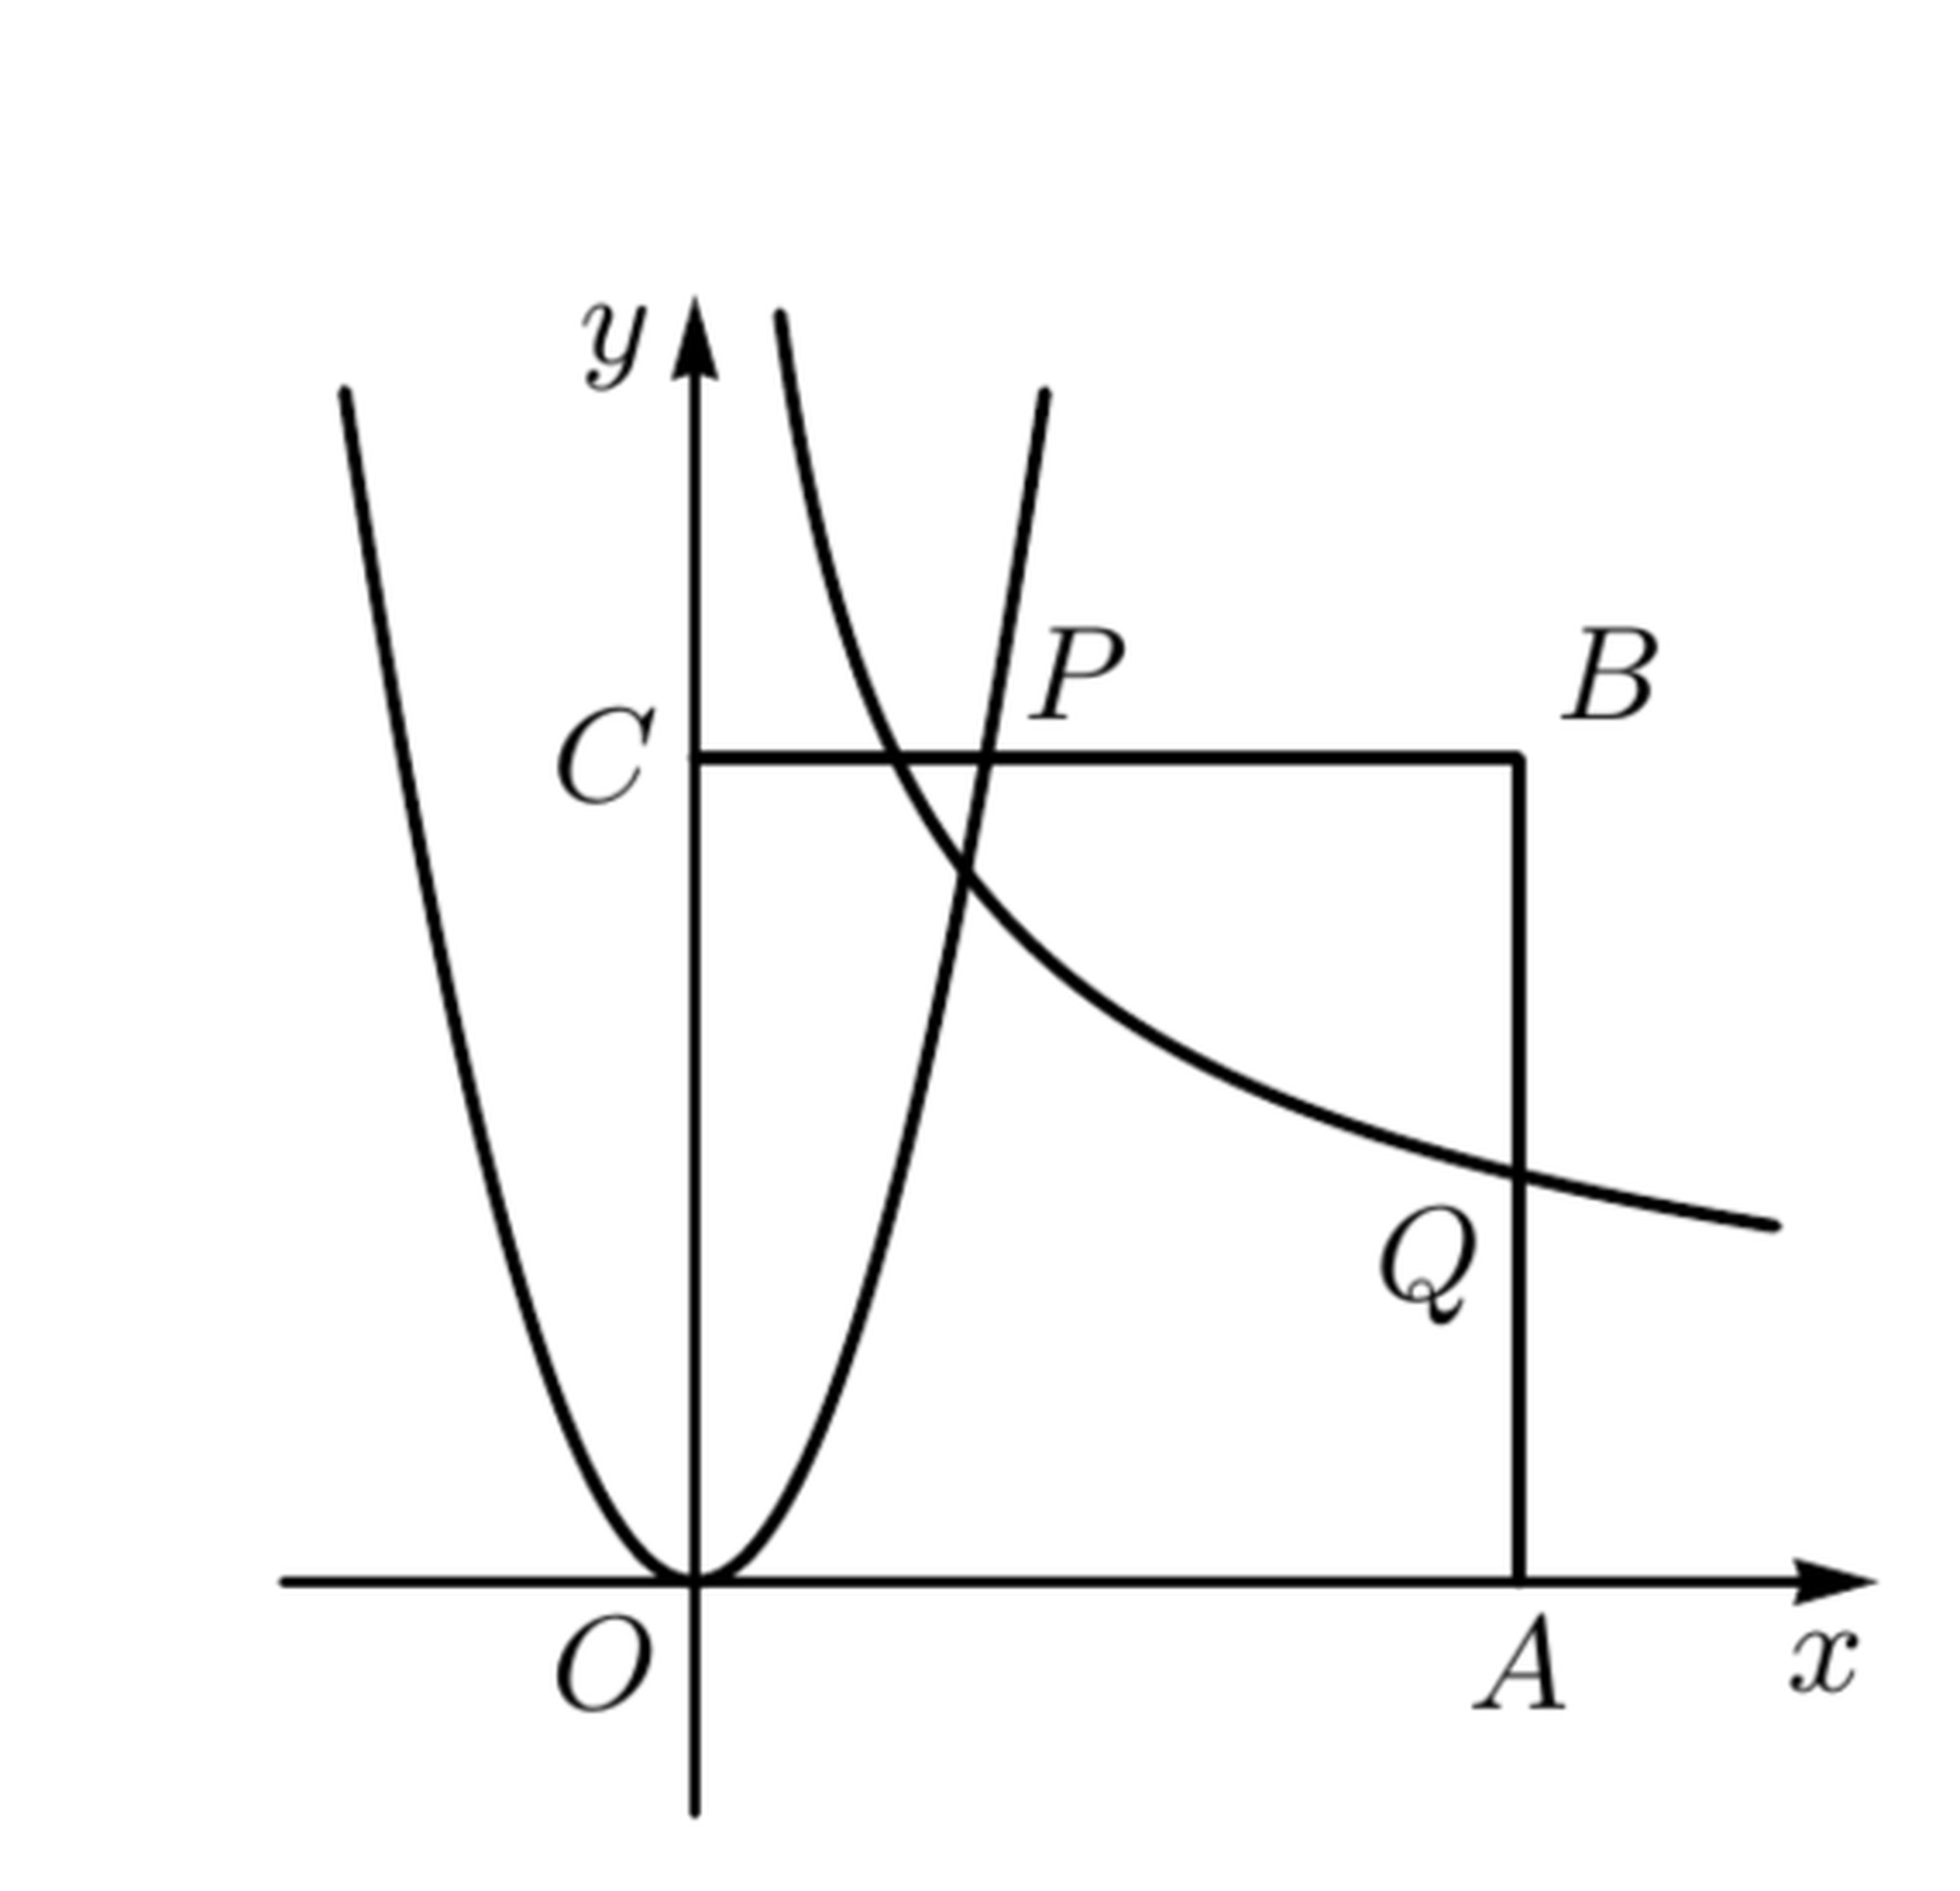
\includegraphics[width=0.40\textwidth]{figures/gao153_q11.png}
\end{center}

\ifanswer
\solbegin
\step{$\lvert AQ\rvert=\dfrac1{\sqrt a}$，$\lvert CP\rvert=\sqrt{\dfrac a5}$，}
\step{于是 $\lvert AQ\rvert+\lvert CP\rvert=\dfrac1{\sqrt a}+\sqrt{\dfrac a5}\geqslant2\sqrt{\dfrac1{\sqrt a}\cdot\sqrt{\dfrac a5}}=\dfrac2{\sqrt[4]{5}}$，}
\step{当且仅当 $\dfrac1{\sqrt a}=\sqrt{\dfrac a5}$，即 $a=\sqrt5$ 时取等号.}
\solend
\fi

% === Q12 === $B\subseteq A$ 带下划线照录、空集 \varnothing；解析 5 行
\item 若集合 $A=\{x\mid1\leqslant x\leqslant100,x\in\Z\}$，集合 $B\subseteq A$，且 $B\ne\varnothing$，记 $W(B)$ 为 $B$ 中元素的最大值与最小值之和，则对所有的 $B$，$W(B)$ 的平均值是\blankline[4.4em].

\ifanswer
\solbegin
\step{对每个非空子集 $B$，令 $B'=\{101-x\mid x\in B\}$，}
\step{则 $W(B')=(101-\min B)+(101-\max B)=202-W(B)$.}
\step{对 $B'$ 再作同样变换即得到 $B$，因此 $B$ 遍历所有非空子集时，}
\step{$B'$ 也恰好遍历所有非空子集.}
\step{设所求平均值为 $m$，则 $m=202-m$，解得 $m=101$.}
\solend
\fi

\end{enumerate}

\bigsec{二、选择题}

\begin{enumerate}
\setcounter{enumi}{12}

% === Q13 === "图像"（像，有亻）照录；解析 2 行，故选 A
\item 设 $a$、$b$ 为常数，若 $0<a<1$，$b>1$，则函数 $y=a^x-b$ 的图像必定不经过\mbox{（\quad）}

\keepwithprev
A. 第一象限\qquad\qquad B. 第二象限\qquad\qquad C. 第三象限\qquad\qquad D. 第四象限

\ifanswer
\solbegin
\step{当 $x>0$ 时，$a^x<1<b$，所以 $y=a^x-b<0$，图像必定不经过第一象限，}
\step{故选 $A$.}
\solend
\fi

% === Q14 === $m\in\Z$、中文弯引号、"图像"照录；解析 3 行，故选 A
\item 已知 $m\in\Z$，则“$m=0$”是“幂函数 $y=x^{m^2-2m-1}$ 的图像与 $x$ 轴及 $y$ 轴均无交点，且关于原点成中心对称”的\mbox{（\quad）}

\keepwithprev
A. 充分不必要条件\qquad\qquad B. 必要不充分条件

C. 充要条件\qquad\qquad D. 既不充分也不必要条件

\ifanswer
\solbegin
\step{图像满足所述条件 $\Leftrightarrow m^2-2m-1$ 为负奇数 $\Leftrightarrow m=0$ 或 $m=2$.}
\step{$m=0$ 能推出所述条件，但所述条件不能推出 $m=0$，因此是充分不必要条件，}
\step{故选 $A$.}
\solend
\fi

% === Q15 === 四选项一行；解析 5 行（跨 03→04 页），故选 D
\item 设 $a>b>1$，$x>1$，则下列不等式正确的是\mbox{（\quad）}

\keepwithprev
A. $a^x<b^x$\qquad B. $x^a<x^b$\qquad C. $\log_a x>\log_b x$\qquad D. $\log_x a>\log_x b$

\ifanswer
\solbegin
\step{$x>1$，幂函数与指数函数的单调性给出 $a^x>b^x$，$x^a>x^b$，A、B 错误.}
\step{$\log_a x=\dfrac{\lg x}{\lg a}<\dfrac{\lg x}{\lg b}=\log_b x$，C 错误.}
\step{对数函数 $y=\log_x t$ 的底数 $x>1$，在 $(0,+\infty)$ 上严格递增，}
\step{所以 $\log_x a>\log_x b$，D 正确.}
\step{故选 $D$.}
\solend
\fi

% === Q16 === $a\in\N$；解析 3 行，故选 C
\item 设 $a\in\N$，则满足不等式 $x^2-a^2x-a^2-1<0$ 的整数 $x$ 的个数不可能是\mbox{（\quad）}

\keepwithprev
A. 1\qquad\qquad B. 50\qquad\qquad C. 100\qquad\qquad D. 2026

\ifanswer
\solbegin
\step{$(x+1)(x-a^2-1)<0\Leftrightarrow-1<x<a^2+1$. 整数解为 $0,1,\cdots,a^2$，共 $a^2+1$ 个.}
\step{$1=0^2+1$，$50=7^2+1$，$2026=45^2+1$，而 $100-1=99$ 不是完全平方数，}
\step{故选 $C$.}
\solend
\fi

\end{enumerate}

\bigsec{三、解答题}

\begin{enumerate}
\setcounter{enumi}{16}

% === Q17 === 补集上划线 \overline{A}、\subseteq 照录；解析 5 行
\item 已知全集 $U=\R$，集合 $A=\{x\mid x^2-x-2\geqslant0\}$，$B=\{x\mid x>-1\}$，$C=\{x\mid a-5<x<a\}$.

(1) 求 $A\cap B$、$A\cup B$；

(2) 若 $\overline{A}\cup C=C$，求实数 $a$ 的取值范围.

\ifanswer
\solbegin
\step{(1) $x^2-x-2=(x+1)(x-2)\geqslant0\Leftrightarrow x\leqslant-1$ 或 $x\geqslant2$，}
\step{所以 $A=(-\infty,-1]\cup[2,+\infty)$，$B=(-1,+\infty)$，}
\step{因此 $A\cap B=[2,+\infty)$，$A\cup B=\R$.}
\step{(2) $\overline{A}=(-1,2)$，于是 $\overline{A}\cup C=C\Leftrightarrow\overline{A}\subseteq C\Leftrightarrow(-1,2)\subseteq(a-5,a)$，}
\step{两区间均为开区间，端点可重合，故 $\begin{cases}a-5\leqslant-1\\a\geqslant2\end{cases}\Leftrightarrow2\leqslant a\leqslant4$.}
\solend
\fi

% === Q18 === 解析 4 行
\item 已知 $a$、$b$、$c$ 都是正数，

(1) 若 $a+b=1$，求证：$\dfrac1a+\dfrac1b\geqslant4$，并指出等号成立的条件；

(2) 若 $a+b+c=1$，求证：三个数 $\dfrac1a$、$\dfrac1b$、$\dfrac1c$ 中至少有一个不小于 3.

\ifanswer
\solbegin
\step{(1) 由 $(a-b)^2\geqslant0$，得 $4ab\leqslant(a+b)^2=1$，所以 $\dfrac1a+\dfrac1b=\dfrac{a+b}{ab}=\dfrac1{ab}\geqslant4$，}
\step{等号成立当且仅当 $a=b$，结合 $a+b=1$，得 $a=b=\dfrac12$.}
\step{(2) 假设三个数 $\dfrac1a$、$\dfrac1b$、$\dfrac1c$ 都小于 3，则 $a>\dfrac13,b>\dfrac13,c>\dfrac13\Rightarrow a+b+c>1$，}
\step{与 $a+b+c=1$ 矛盾，因此三个数中至少有一个不小于 3.}
\solend
\fi

% === Q19 === 题目配图（三版都出）；\needvspace 守卫放 \item 之前；解析 19 行
\needvspace{8cm}
\item 某新建居民小区有一直角三角形绿地，两直角边长分别为 30m 和 40m，打算在其中划出一片区域改造成活动场地，如图所示.

(1) 若划出的区域为正方形，且有两边落在绿地边界上，求此正方形边长；

(2) 若划出的区域为圆形，求圆形区域面积的最大值；

(3) 若划出的区域为矩形（其中至少有一边在边界上），求此矩形面积的最大值.

\begin{center}
% 直角三角形 ABC 绿地示意图取 05 页右上，去粉色水印、去色、4× LANCZOS 放大；三版都出
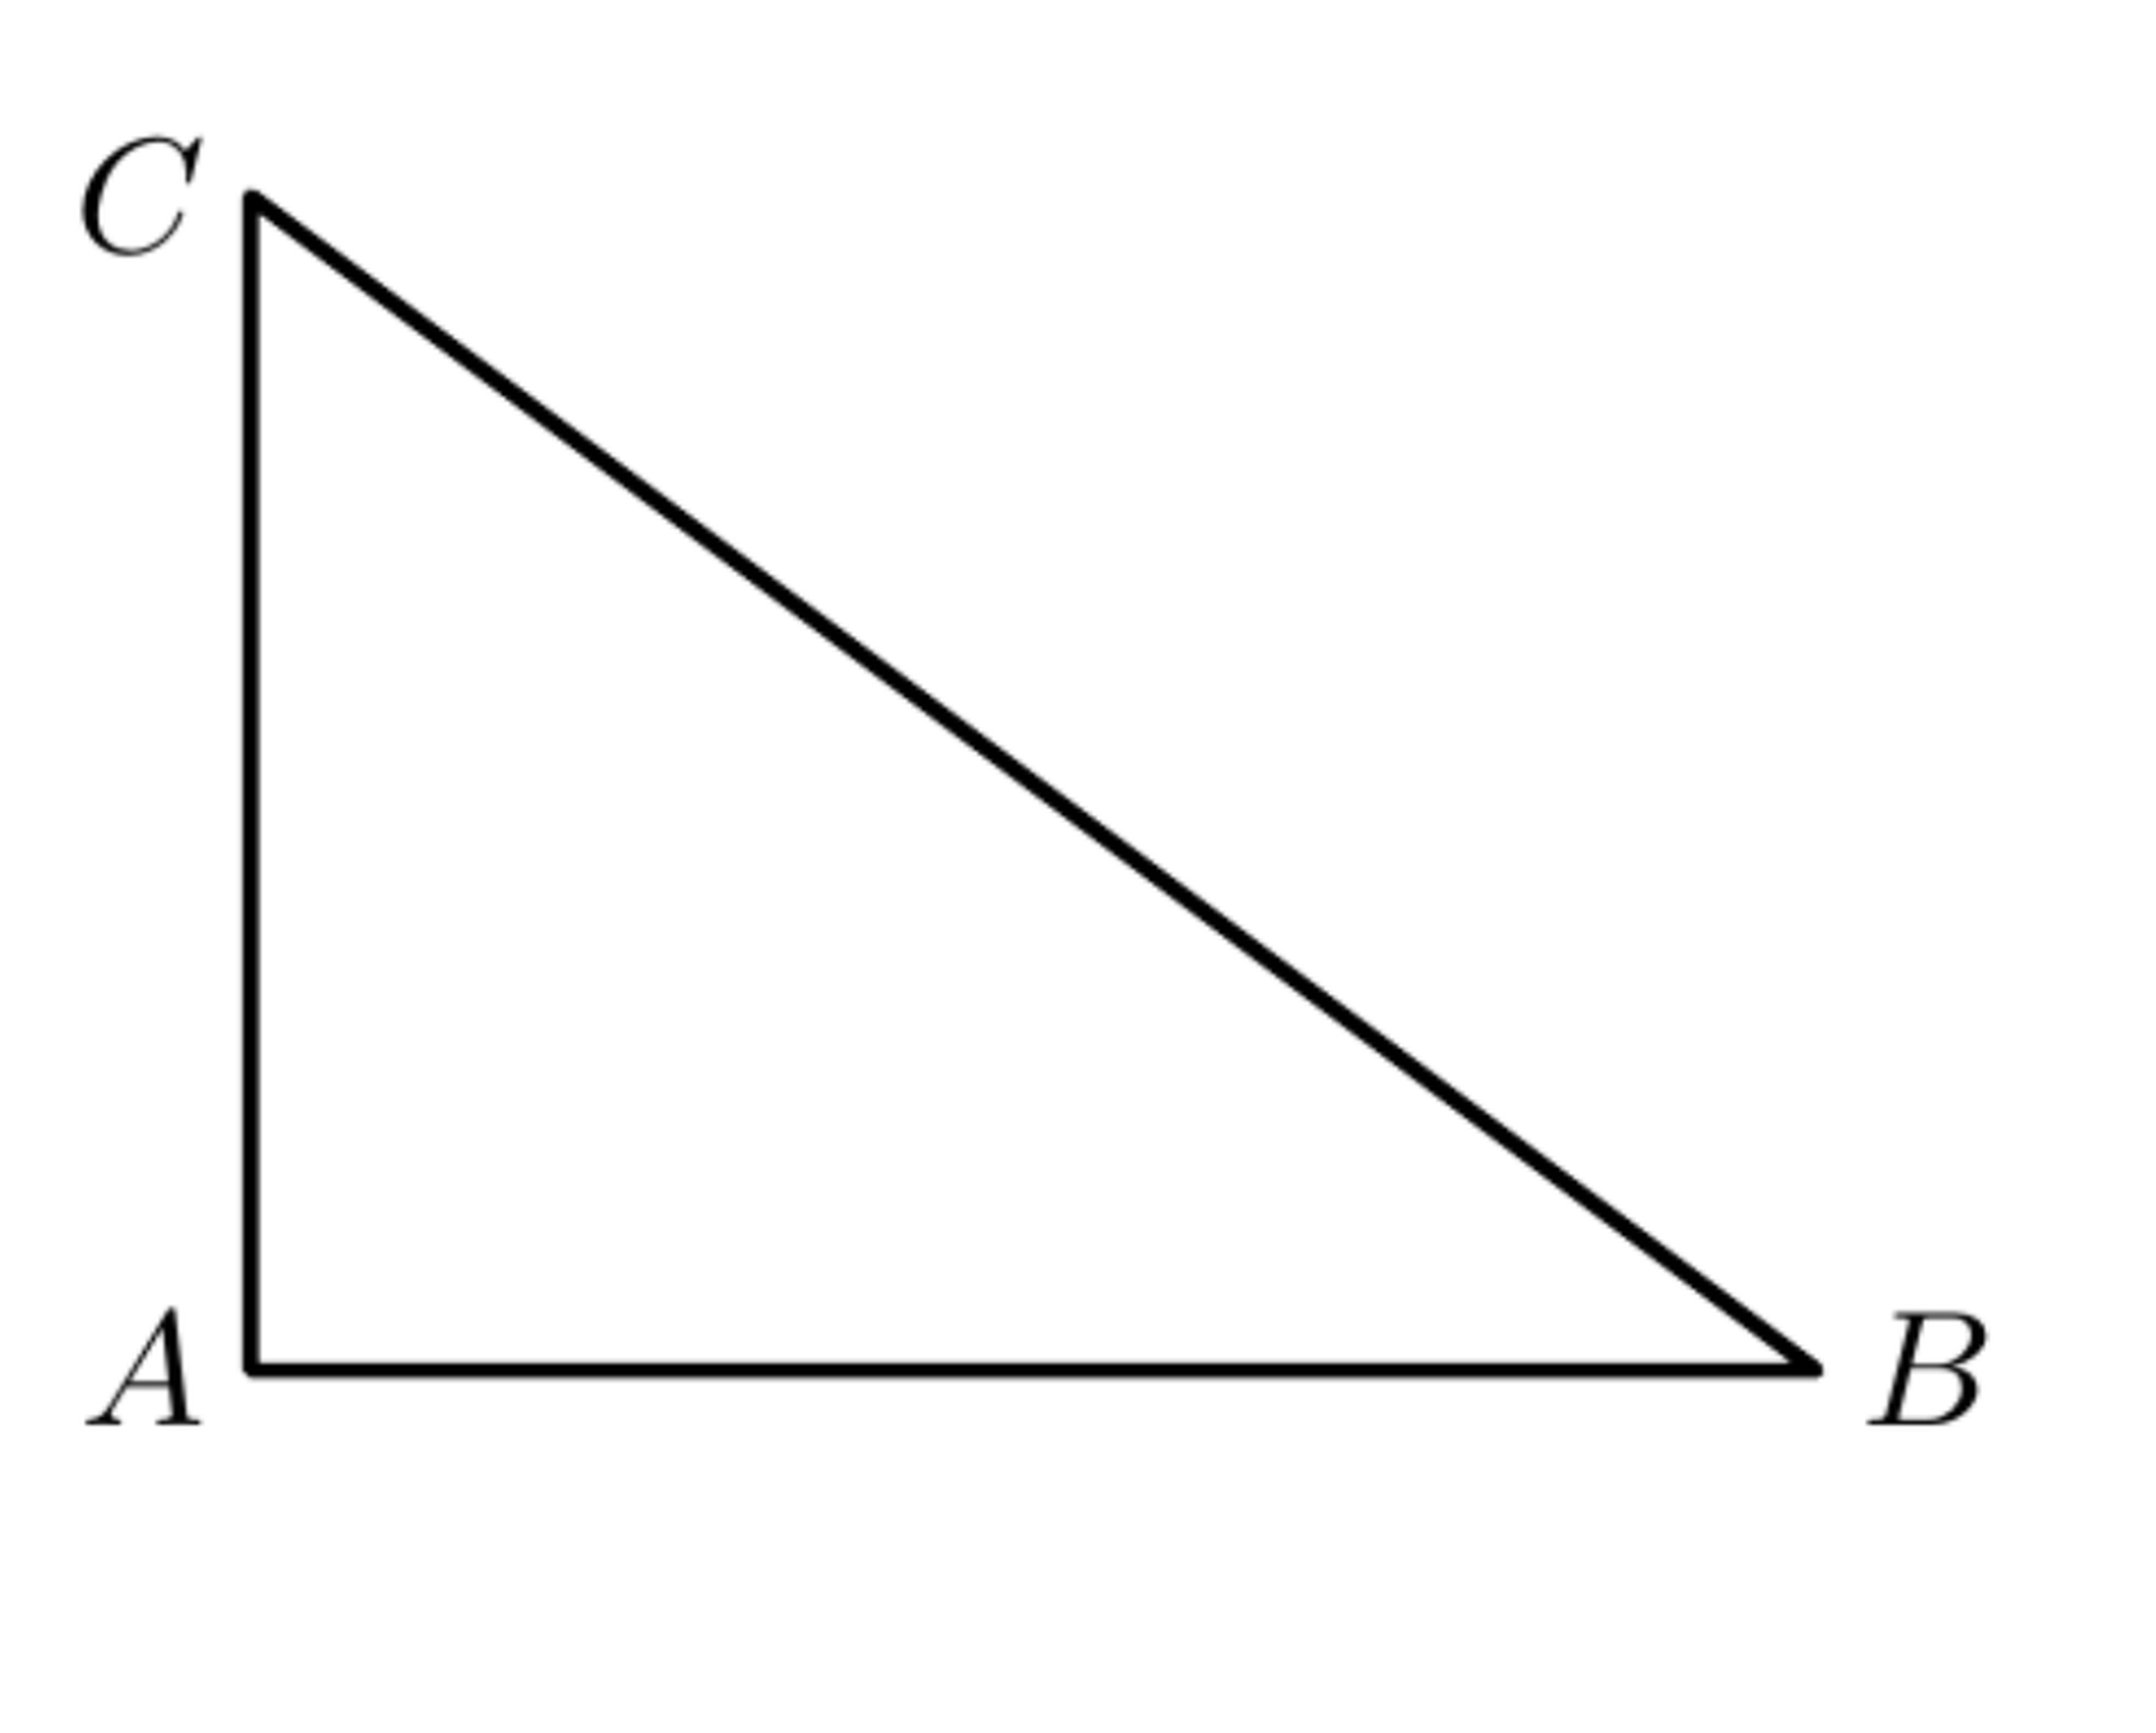
\includegraphics[width=0.34\textwidth]{figures/gao153_q19.png}
\end{center}

\ifanswer
\solbegin
\step{(1) 取 $A(0,0)$、$B(40,0)$、$C(0,30)$，则斜边 $BC$ 所在直线为 $3x+4y=120$.}
\step{正方形落在边界上的两边必分别在两条直角边上.}
\step{设其边长为 $a$m，则对角顶点为 $(a,a)$.}
\step{按题意划出的正方形应尽量大，即对角顶点落在斜边 $BC$ 上，}
\step{因此 $3a+4a=120\Rightarrow a=\dfrac{120}{7}$；}
\step{(2) 斜边长 $BC=\sqrt{30^2+40^2}=50$m，三角形面积为 $600\text{m}^2$.}
\step{设圆的半径为 $r$，圆心到 $AB$、$AC$、$BC$ 的距离分别为 $d_1,d_2,d_3$，}
\step{则三者均不小于 $r$. 连接圆心与三个顶点，}
\step{得 $600=\dfrac12(40d_1+30d_2+50d_3)\geqslant\dfrac12(40+30+50)r=60r$，所以 $r\leqslant10$.}
\step{取三角形的内切圆时等号成立，圆形区域面积的最大值为 $100\pi\text{m}^2$.}
\step{(3) 任取矩形落在绿地边界上的一边，以其所在直线为横轴.}
\step{设相应三角形底边长为 $L$、高为 $H$，则 $LH=1200$.}
\step{取三角形顶点坐标为 $(0,0)$、$(L,0)$、$(p,H)$.}
\step{在高度 $t$ 处，两腰上的点的横坐标分别为 $\dfrac{pt}{H}$、$L+\dfrac{(p-L)t}{H}$，}
\step{因此，高为 $t$ 的矩形，其底边长不超过 $L\left(1-\dfrac tH\right)$，}
\step{面积满足 $S\leqslant Lt\left(1-\dfrac tH\right)=\dfrac LH\left[\dfrac{H^2}{4}-\left(t-\dfrac H2\right)^2\right]\leqslant\dfrac{LH}{4}=300$，}
\step{在原坐标系中，取矩形顶点为 $(0,0)$、$(20,0)$、$(20,15)$、$(0,15)$，}
\step{其中 $3\times20+4\times15=120$，矩形完全位于绿地内，面积为 $300\text{m}^2$，}
\step{达到最大值.}
\solend
\fi

% === Q20 === $g(x)$ 定义照录；解析 14 行
\item 已知 $a>0$ 且 $a\ne1$，设 $f(x)=\log_a(x^2-a^2)$，$g(x)=2\log_a(x-ak)$.

(1) 求函数 $y=f(x)$ 的定义域；

(2) 若 $k=2$，求不等式 $f(x)>g(x)$ 的解集；

(3) 若“存在实数 $x$，使得 $f(x)=g(x)$”为真命题，求实数 $k$ 的取值范围.

\ifanswer
\solbegin
\step{(1) $x^2-a^2>0\Leftrightarrow x<-a$ 或 $x>a$，定义域为 $(-\infty,-a)\cup(a,+\infty)$.}
\step{(2) 两函数均有意义时，$x>2a$，且 $g(x)=\log_a(x-2a)^2$.}
\step{当 $a>1$ 时，$f(x)>g(x)\Leftrightarrow x^2-a^2>(x-2a)^2\Leftrightarrow x>\dfrac{5a}{4}$，}
\step{结合 $x>2a$，解集为 $(2a,+\infty)$.}
\step{当 $0<a<1$ 时，$f(x)>g(x)\Leftrightarrow x^2-a^2<(x-2a)^2\Leftrightarrow x<\dfrac{5a}{4}$，}
\step{与 $x>2a$ 矛盾，解集为 $\varnothing$.}
\step{(3) 在 $x^2-a^2>0$ 且 $x-ak>0$ 的条件下，}
\step{$f(x)=g(x)\Leftrightarrow x^2-a^2=(x-ak)^2\Leftrightarrow2akx=a^2(1+k^2)$，}
\step{当 $k=0$ 时，上式不成立；}
\step{当 $k\ne0$ 时，$x=\dfrac{a(1+k^2)}{2k}$，}
\step{于是 $x-ak=\dfrac{a(1-k^2)}{2k}>0\Leftrightarrow k<-1$ 或 $0<k<1$，}
\step{对上述 $k$，所取的 $x$ 同时满足 $x^2-a^2=(x-ak)^2>0$，}
\step{两函数均有意义且函数值相等.}
\step{因此，$k$ 的取值范围为 $(-\infty,-1)\cup(0,1)$.}
\solend
\fi

% === Q21 === 中文弯引号、复杂式照录；解析 23 行（跨 08→09 页）
\item 若实数 $x$、$y$、$m$ 满足 $\lvert x-m\rvert<\lvert y-m\rvert$，则称 $x$ 比 $y$ 接近 $m$.

(1) 若 $2x$ 比 $x-2$ 更接近 1，求实数 $x$ 的取值范围；

(2) 若 $x$ 比 $y$ 接近 $m$，证明：“$x>y$” 的充要条件是 “$x+y<2m$”；

(3) 已知 $x>0$，$y>0$ 且 $x\ne y$. 设 $p=\dfrac{x^2+y^2}{xy}$，若对于任意的 $x$、$y$，命题 “$p$ 比 $p^2-3p+4$ 接近 $m$” 恒成立，求实数 $m$ 的取值范围.

\ifanswer
\solbegin
\step{(1) $\lvert2x-1\rvert<\lvert x-3\rvert\Leftrightarrow(2x-1)^2<(x-3)^2\Leftrightarrow(x+2)(3x-4)<0$，}
\step{解得 $-2<x<\dfrac43$，实数 $x$ 的取值范围为 $\left(-2,\dfrac43\right)$.}
\step{(2) 因为 $x$ 比 $y$ 接近 $m$，所以 $\lvert x-m\rvert<\lvert y-m\rvert$，则 $\lvert x-m\rvert^2<\lvert y-m\rvert^2$，}
\step{即 $(x-m)^2<(y-m)^2$，即 $(x-m)^2-(y-m)^2<0$，}
\step{即得 $(x-y)(x+y-2m)<0$，}
\step{则由 $x+y<2m$，得 $x+y-2m<0$，}
\step{故 $x-y>0$，即 $x>y$，充分性成立；}
\step{当 $x>y$ 时，$x-y>0$，结合 $(x-y)(x+y-2m)<0$，得 $x+y-2m<0$，}
\step{即 $x+y<2m$，必要性成立；}
\step{故“$x>y$” 的充要条件是 “$x+y<2m$”；}
\step{(3) $x>0$，$y>0$ 且 $x\ne y$. 则 $p=\dfrac{x^2+y^2}{xy}=\dfrac xy+\dfrac yx>2\sqrt{\dfrac xy\cdot\dfrac yx}=2$，}
\step{由于对于任意的 $x$、$y$，命题 “$p$ 比 $p^2-3p+4$ 接近 $m$” 恒成立，}
\step{故 $\lvert p-m\rvert<\lvert(p^2-3p+4)-m\rvert$ 对 $\forall p>2$ 恒成立，}
\step{即得 $(p-m)^2<(p^2-3p+4-m)^2$，}
\step{即 $(p^2-3p+4-m)^2-(p-m)^2>0$，}
\step{得 $(p^2-4p+4)(p^2-2p+4-2m)>0$，}
\step{即 $(p-2)^2(p^2-2p+4-2m)>0$，由于 $p>2$，故 $(p-2)^2>0$，}
\step{故 $p^2-2p+4-2m>0$ 对 $\forall p>2$ 恒成立，}
\step{即 $2m<p^2-2p+4$ 对 $\forall p>2$ 恒成立，}
\step{由于 $p^2-2p+4=(p-1)^2+3$，此时 $p^2-2p+4$ 在 $(2,+\infty)$ 上严格增，}
\step{故 $(p-1)^2+3>(2-1)^2+3=4$，故 $2m\leqslant4$，解得 $m\leqslant2$，}
\step{即实数 $m$ 的取值范围是 $(-\infty,2]$.}
\solend
\fi

\end{enumerate}

\end{document}
"
% 紧凑版：xelatex "\def\iscompact{1}% 高一153_闵行中学文绮中学_期中.tex
%   —— 高一上数学"2026-2027 年闵行中学文绮中学高一上期中"（试卷版/答案版/紧凑版）
% 试卷版：xelatex 高一153_闵行中学文绮中学_期中.tex
% 答案版：xelatex "\def\isanswer{1}% 高一153_闵行中学文绮中学_期中.tex
%   —— 高一上数学"2026-2027 年闵行中学文绮中学高一上期中"（试卷版/答案版/紧凑版）
% 试卷版：xelatex 高一153_闵行中学文绮中学_期中.tex
% 答案版：xelatex "\def\isanswer{1}% 高一153_闵行中学文绮中学_期中.tex
%   —— 高一上数学"2026-2027 年闵行中学文绮中学高一上期中"（试卷版/答案版/紧凑版）
% 试卷版：xelatex 高一153_闵行中学文绮中学_期中.tex
% 答案版：xelatex "\def\isanswer{1}\input{高一153_闵行中学文绮中学_期中.tex}"
% 紧凑版：xelatex "\def\iscompact{1}\input{高一153_闵行中学文绮中学_期中.tex}"
%
% ① 原始材料：微信公众号"魔都数学加油站"文章，连载"27学年高一153"，原文标题
% "27学年高一153——2026-2027年上海市闵行中学文绮中学高一上期中"；
% 原文链接：https://mp.weixin.qq.com/s/rEtS-92cDR6JKgY2b5DRfg 。
% 正文为 9 张 PNG 页（01/02/06/07/08/09 为 2560×3620，03/04/05 为 4762×6735，
% 同一篇各页分辨率混排，逐页按各自分辨率裁图核对，别按预览比例换算裁框）。
% 体例：讲评版——填空 3—12（10 题）、选择 13—16（4 题）、解答 17—21（5 题），
% 共 19 题，自第 3 题起编；**全 19 题均印【解析】**（逐题核实，见 ② ②）。
% 题目、答案、解析均据原图转录；卷面粉红色水印"魔都数学加油站"及公众号页脚未录入。
% 全卷插图清单（逐页通读 9 页确认）：2 幅，均为题目配图、三版都出——
%   · Q11 正方形 OABC 曲线图（02 页右下：$y=5x^2$ 与 $y=x^{-\frac12}$ 两条曲线、
%     坐标轴、O/A/B/C/P/Q、正方形），裁 figures/gao153_q11.png；
%   · Q19 直角三角形 ABC 绿地示意图（05 页右上，直角在 A），
%     裁 figures/gao153_q19.png；
%   两图均去粉色水印、去色、4× LANCZOS 放大；Q11 图左上角题干残字"函"已裁白。
%   其余各页逐页确认无其它题目配图、无解析内配图、无表格；09 页下半仅水印、无正文。
%
% 卷首标题：原卷印作"2026-2027 年闵行中学文绮中学高一上期中"，年份区间按全稿惯例排 en dash；
% 原卷卷面未印副标题，本稿按同期中卷知识模块口径补出"集合与常用逻辑用语、不等式、函数"。
%
% ② 与原卷的排版差异：
%   ① 原文从第 3 题起，本稿保留原题号；共 19 题三节，解答题 5 题到 21；
%   ② 全 19 题均印【解析】、用 \solbegin…\solend，无只印【答案】或答案印括号内的题；
%      四道选择题答案在解析末句"故选 A／A／D／C"（Q13—Q16，逐个放大复核）、
%      括号 \mbox{（\quad）} 留空、不另提 \ans{}；答案版【答案】/【解析】标记数
%      = 19 = 全卷题数；
%   ③ 原卷卷面未印副标题，本稿按知识模块口径补出；
%   ④ 原卷填空横线按全稿惯例排 \blankline[4.4em]；选择题括号排 \mbox{（\quad）}、
%      四道选择题的选项段前按惯例各加 \keepwithprev；解答题不留作答区、不加
%      \anspace（原卷为讲评版，109—113 起全稿不用 \anspace）；
%   ⑤ 数集：Q3"$x\in R$"、Q5"解集为 R"、Q10"$x\in N$"、Q12"$x\in Z$"与
%      "$m\in Z$"、Q14"$m\in Z$"、Q16"$a\in N$"、Q17"全集 $U=R$"、
%      Q19 无、Q21 无——原卷印斜体或正体粗体 R/N/Z，按全稿惯例归一
%      \R／\N／\Z；绝对值排 \lvert…\rvert（Q5、Q11、Q21），集合描述竖线排 \mid
%      （Q3、Q10、Q17、Q20），不等号按全稿惯例排 \leqslant／\geqslant；
%      补集照原卷上划线排 \overline{A}（Q17 题干 (2)＋解析 (2)）；
%      空集 \varnothing（Q12 题干、Q20 解析 (2)）；子集 3 处均印带下划线 ⊆、
%      照录 \subseteq（Q10 $A\subseteq U$、Q12 $B\subseteq A$、Q17 $(-1,2)\subseteq(a-5,a)$），
%      本卷无单线 \subset 用例；
%   ⑥ 判别式：逐页通读 9 页，本卷无一元二次判别式 Δ/△ 算式，故无 Δ/△ 混用可照录；
%      Q11 图里有几何正方形 OABC（非三角形符号），无 △ABC 用例；
%   ⑦ 中文弯引号照录：Q14"$m=0$"与"幂函数…关于原点成中心对称"、
%      Q20"存在实数 $x$，使得 $f(x)=g(x)$"、Q21"$x>y$"与"$x+y<2m$"、
%      "$p$ 比 $p^2-3p+4$ 接近 $m$"（引号外留空格按原卷）；
%      注释里一律 ASCII 引号；数学式内 CJK 用 \text{}；
%   ⑧ "图像／图象"逐处放大核：全卷 3 处均印"图像"（像，有亻）——
%      Q13 题干与解析、Q14 题干与解析；Q19 题干写"如图所示"（非"图像"），
%      逐处照录未统一；子题标号 (1)(2)(3) 半角括号照录；圈数字本卷无用例；
%   ⑨ 半角逗号在数学组之间是全稿惯例、非笔误，逐处照录（Q3 $x\in R$、
%      Q10 $a_1,a_2$、Q19 $A(0,0)$、$d_1,d_2,d_3$、Q21 $a>\frac13,b>\frac13$ 等）；
%      行末西文句点 ASCII `.`；行中全角逗号／顿号照录（Q19"30m 和 40m"、
%      Q21"实数 $x$、$y$、$m$"）；
%   ⑩ 复杂式照录别简化：Q3 $y=x^{-2}$、Q11 $y=x^{-\frac12}$ 与
%      $\frac{2}{\sqrt[4]{5}}$、Q8 $\frac{2b}{a+1-b}$、Q9 cases 块、
%      Q10 $525=5\times105$、Q16 $a^2+1$、Q19 $S\leqslant Lt(1-\frac tH)$
%      与 $L+\frac{(p-L)t}{H}$、Q20 $2akx=a^2(1+k^2)$ 与 $\frac{a(1+k^2)}{2k}$、
%      Q21 $(p^2-4p+4)(p^2-2p+4-2m)>0$；
%      \left…\right 不得拆到不同 $…$ 组（Q17 $\left\{x\mid\cdots\right\}$、
%      Q19 $\left[\frac{H^2}{4}-\left(t-\frac H2\right)^2\right]$、
%      Q21 $\left(-2,\frac43\right)$ 等）；cases 块一律 \begin{cases}…\end{cases}；
%   ⑪ 一条 \step = 原卷解析的一个印刷行，cases 块整体算一个印刷行；别并折行、
%      别拆行。Q10 六行、Q19 十九行、Q20 十四行、Q21 二十二行均按印刷行逐条断，
%      不丢行；
%   ⑫ 配图：Q11／Q19 题目配图（三版都出）放 \item 内题干之后 \begin{center}，
%      各用 \needvspace{8cm} 守卫把整块推走，**守卫放在 \item 之前**
%      （见 高一145 Q14/Q20 成例与切页审计 B 类坑）；
%   ⑬ 原卷解析内无红色"法一／法二"之类小标题，故本卷无 \stepm；红色水印
%      "魔都数学加油站"不录入；
%   ⑭ 跨页续印按题合并：见 ⑥；
%
% ③ 行数复核：一条 \step = 原卷解析的一个印刷行，cases 块作一个印刷行计。
%   逐题数（主会话逐页核对定稿）：Q3：1；Q4：2；Q5：2；Q6：2；Q7：1；
%   Q8：1；Q9：2；Q10：6；Q11：3；Q12：5；Q13：2；Q14：3；Q15：5；
%   Q16：3；Q17：5；Q18：4；Q19：19；Q20：14；Q21：22。
%   合计 102 条 \step（本卷无 \stepm），与原卷逐题印刷行相等。全卷 19 题
%   均设 \solbegin…\solend，答案版【答案】/【解析】标记数 = 19 = 全卷题数。
%
% ④ 判别式／子集符号结论（逐处放大原图照录、不得统一，主会话像素级复核）：
%   判别式：逐页通读 9 页，本卷无一元二次判别式算式（Q7 用韦达定理、
%      Q16 用因式分解、Q20 用对数方程，均不写 Δ/△），故无 Δ/△ 混用可照录
%      （"高 \Delta／扁 \triangle"口径备查，参照 高一142／151／152 头注）；
%      本卷无几何三角形符号用例。
%   子集：Q10 题干"$A\subseteq U$"、Q12 题干"$B\subseteq A$"、Q17 解析 (2)
%      "$(-1,2)\subseteq(a-5,a)$"共 3 处，逐处放大确认均印带下划线 ⊆、
%      照录 \subseteq；本卷未见单线 ⊂（\subset）之对应处。
%      补集上划线 \overline{A}（Q17）、空集 \varnothing（Q12 题干、Q20 解析 (2)）；
%      数集 \R／\N／\Z 归一见 ② ⑤。
%
% ⑤ 存疑照录（放大原图确认，照录未改、正文对应处另有 % 注）：
%   1. Q3 集合 $B=\{(x,y)\mid y=x^{-2},x\in\R\}$ 原卷题干径写 $x\in\R$
%      （$x=0$ 处无意义），解析自行注明 $x\ne0$，照录未改。
%   2. Q10 解析"$U$ 中共有 $525=5\times105$ 个连续整数"与尾行
%      "取 $U$ 中除以 5 余 1 或 2 的全部元素及元素 5"逐字照录（放大 02 页
%      /tmp/gao153/z/zoom/q10_pick.png 确认是"元素 5"，非"元素 9"）。
%   3. Q11 第二个函数原卷印 $y=x^{-\frac12}$（负二分之一次幂，非 $x^2$），
%      放大 02 页 /tmp/gao153/z/zoom/q11_exp.png 确认，照录未改；
%      $|AQ|=\frac1{\sqrt a}$ 与之自洽。
%   4. Q19 (3) 解析"在高度 $t$ 处，两腰上的点的横坐标分别为 $\frac{pt}{H}$、
%      $L+\frac{(p-L)t}{H}$"，放大 06 页确认，照录未简化。
%   5. Q20 (2) 解析"$g(x)=\log_a(x-2a)^2$"（真数整体平方），
%      与 $g(x)=2\log_a(x-ak)$ 在 $k=2$ 时一致，照录未改。
%   6. Q21 (3) 解析"得 $(p^2-4p+4)(p^2-2p+4-2m)>0$"与
%      "故 $(p-1)^2+3>(2-1)^2+3=4$，故 $2m\leqslant4$"照录未改
%      （放大 09 页 /tmp/gao153/z/zoom/q21_factor.png 确认）。
%   7. "图像／图象"全卷 3 处均印"图像"（像，有亻）逐处照录；
%      本卷无判别式 Δ/△ 用例（见 ④）。
%   全卷除此 7 类外未发现其它笔误／自相矛盾处；19 题均印【解析】、
%   无只印【答案】或答案印括号内的题（见 ② ②）。
%
% ⑥ 跨页续印按题合并说明（逐页核实定稿）：Q3—Q5 题干＋解析在 01 页；
%   Q6—Q8 题干＋解析在 01 页下半（Q8 解析续 02 页顶）；Q9 题干＋解析、
%   Q10 题干＋解析首 2 行在 02 页上半，Q10 解析余 4 行在 02 页下半；
%   Q11 题干＋配图＋解析、Q12 题干＋解析 5 行在 02 页下半—03 页上半；
%   "二、选择题"标题在 03 页中部；Q13 题干＋选项＋解析在 03 页下半；
%   Q14 题干＋选项＋解析、Q15 题干＋选项＋解析首行在 03 页下半—04 页顶；
%   Q15 解析余 4 行、Q16 题干＋选项＋解析在 04 页上半；"三、解答题"
%   标题在 04 页下半；Q17 题干＋两问＋解析 5 行在 04 页下半—05 页顶；
%   Q18 题干＋两问＋解析 4 行、Q19 题干（含配图）＋三问在 05 页；
%   Q19 解析 (1)(2) 9 行在 05 页下半，解析 (3) 前 5 行在 06 页上半、
%   余 4 行在 06 页下半；Q20 题干＋三问在 06 页下半，解析 (1)(2)(3)
%   前 6 行在 07 页上半、(3) 余 8 行在 07 页下半；Q21 题干＋三问在
%   07 页末，解析 (1)(2) 10 行在 08 页上半—下半，解析 (3) 前 4 行在
%   08 页下半、余 9 行续 09 页上半，末行"即实数 $m$ 的取值范围是
%   $(-\infty,2]$"为全卷收尾（09 页下半仅水印、无正文）。
%   本稿按题连排，不丢行、不并折行；全卷末题为第 21 题，无附加题节。
%
\documentclass[a4paper,11pt]{article}
\usepackage{common}

\begin{document}

\examtitlest[3]{2026--2027 年闵行中学文绮中学高一上期中}{集合与常用逻辑用语、不等式、函数}

\bigsec{一、填空题}

\begin{enumerate}
\setcounter{enumi}{2}

% === Q3 === 集合描述竖线 \mid；$y=x^{-2}$ 照录；解析 1 行
\item 已知 $A=\{(x,y)\mid y=x^3,x\in\R\}$，$B=\{(x,y)\mid y=x^{-2},x\in\R\}$，则 $A\cap B=$\blankline[4.4em].

\ifanswer
\solbegin
\step{$x^3=x^{-2}\ (x\ne0)\Leftrightarrow x^5=1\Leftrightarrow x=1$，此时 $y=1$，所以 $A\cap B=\{(1,1)\}$.}
\solend
\fi

% === Q4 === 解析 2 行
\item 若关于 $x$ 的不等式 $\dfrac{x-a}{x+1}>0$ 的解集为 $(-\infty,-1)\cup(4,+\infty)$，则实数 $a=$\blankline[4.4em].

\ifanswer
\solbegin
\step{关于 $x$ 的不等式 $\dfrac{x-a}{x+1}>0$ 即 $(x+1)(x-a)>0$.}
\step{再由它的解集为 $(-\infty,-1)\cup(4,+\infty)$，得 $-1$ 和 4 是 $(x+1)(x-a)=0$ 的两个实数根，故 $a=4$.}
\solend
\fi

% === Q5 === 绝对值 \lvert…\rvert；解析 2 行
\item 若关于 $x$ 的不等式 $\lvert x+1\rvert+\lvert x-2\rvert>m$ 的解集为 $\R$，则实数 $m$ 的取值范围是\blankline[4.4em].

\ifanswer
\solbegin
\step{$\lvert x+1\rvert+\lvert x-2\rvert\geqslant\lvert(x+1)-(x-2)\rvert=3$，当且仅当 $-1\leqslant x\leqslant2$ 时取等号，}
\step{因此 $m<3$.}
\solend
\fi

% === Q6 === 解析 2 行
\item 已知指数函数 $y=a^x$（$a>1$）在区间 $[-1,1]$ 上的最大值比最小值大 $\dfrac32$，则实数 $a=$\blankline[4.4em].

\ifanswer
\solbegin
\step{$a>1$，指数函数在 $[-1,1]$ 上严格增，故 $a-\dfrac1a=\dfrac32\Leftrightarrow(a-2)(2a+1)=0$.}
\step{结合 $a>1$，得 $a=2$.}
\solend
\fi

% === Q7 === 韦达定理；解析 1 行
\item 已知关于 $x$ 的一元二次方程 $x^2+px+2p=0$ 的两个实数根分别为 $x_1$、$x_2$，且 $(x_1+1)(x_2+1)=0$，则 $p=$\blankline[4.4em].

\ifanswer
\solbegin
\step{$0=(x_1+1)(x_2+1)=x_1x_2+x_1+x_2+1=2p-p+1=p+1\Rightarrow p=-1$.}
\solend
\fi

% === Q8 === 换底公式；解析 1 行
\item 已知 $10^a=3$，$\lg5=b$，则 $\log_6 25=$\blankline[4.4em]（用关于 $a,b$ 的关系式表示）.

\ifanswer
\solbegin
\step{$\lg3=a$，$\lg2=1-b$，所以 $\log_6 25=\dfrac{\lg25}{\lg6}=\dfrac{2b}{a+1-b}$.}
\solend
\fi

% === Q9 === cases 块整体算一个印刷行；解析 2 行
\item 已知 $A=[2,5]$，若对任意 $x\in A$，总有 $\dfrac{k}{x}\in A$，则正数 $k=$\blankline[4.4em].

\ifanswer
\solbegin
\step{$k>0$，当 $x\in[2,5]$ 时，$\dfrac{k}{x}$ 的取值范围为 $\left[\dfrac k5,\dfrac k2\right]$，}
\step{因此 $\begin{cases}\dfrac k5\geqslant2\\\dfrac k2\leqslant5\end{cases}\Leftrightarrow10\leqslant k\leqslant10\Leftrightarrow k=10$.}
\solend
\fi

% === Q10 === $A\subseteq U$ 带下划线照录；解析 6 行
\item 已知集合 $U=\{x\mid4\leqslant x\leqslant528,x\in\N\}$，$A=\{a_1,a_2,a_3,\cdots,a_n\}$，且 $A\subseteq U$. 如果集合 $A$ 中的任意两个不同元素之和都不能被 5 整除，则正整数 $n$ 的最大值为\blankline[4.4em].

\ifanswer
\solbegin
\step{$U$ 中共有 $525=5\times105$ 个连续整数，按除以 5 的余数分成五类，}
\step{每类均有 105 个元素.}
\step{余数为 1,4 的两类不能同时选取，余数为 2,3 的两类也不能同时选取，}
\step{余数为 0 的一类最多选 1 个，因此 $n\leqslant105+105+1=211$.}
\step{取 $U$ 中除以 5 余 1 或 2 的全部元素及元素 5，}% 放大 02 页确认是「元素 5」（非 9），照录未改（见 ⑤ 2）
\step{任意两个不同元素之和均不能被 5 整除，此时 $n=211$，最大值为 211.}
\solend
\fi

% === Q11 === 题目配图（三版都出）；\needvspace 守卫放 \item 之前；$y=x^{-\frac12}$ 照录；解析 3 行
\needvspace{8cm}
\item 如图，已知正方形 $OABC$，其中 $OA=a$（$a>1$），函数 $y=5x^2$ 交 $BC$ 于点 $P$，函数 $y=x^{-\frac12}$ 交 $AB$ 于点 $Q$，当 $\lvert AQ\rvert+\lvert CP\rvert$ 最小时，$a$ 的值为\blankline[4.4em].

\begin{center}
% 正方形 OABC 与两条曲线图取 02 页右下，去粉色水印、去色、4× LANCZOS 放大；三版都出
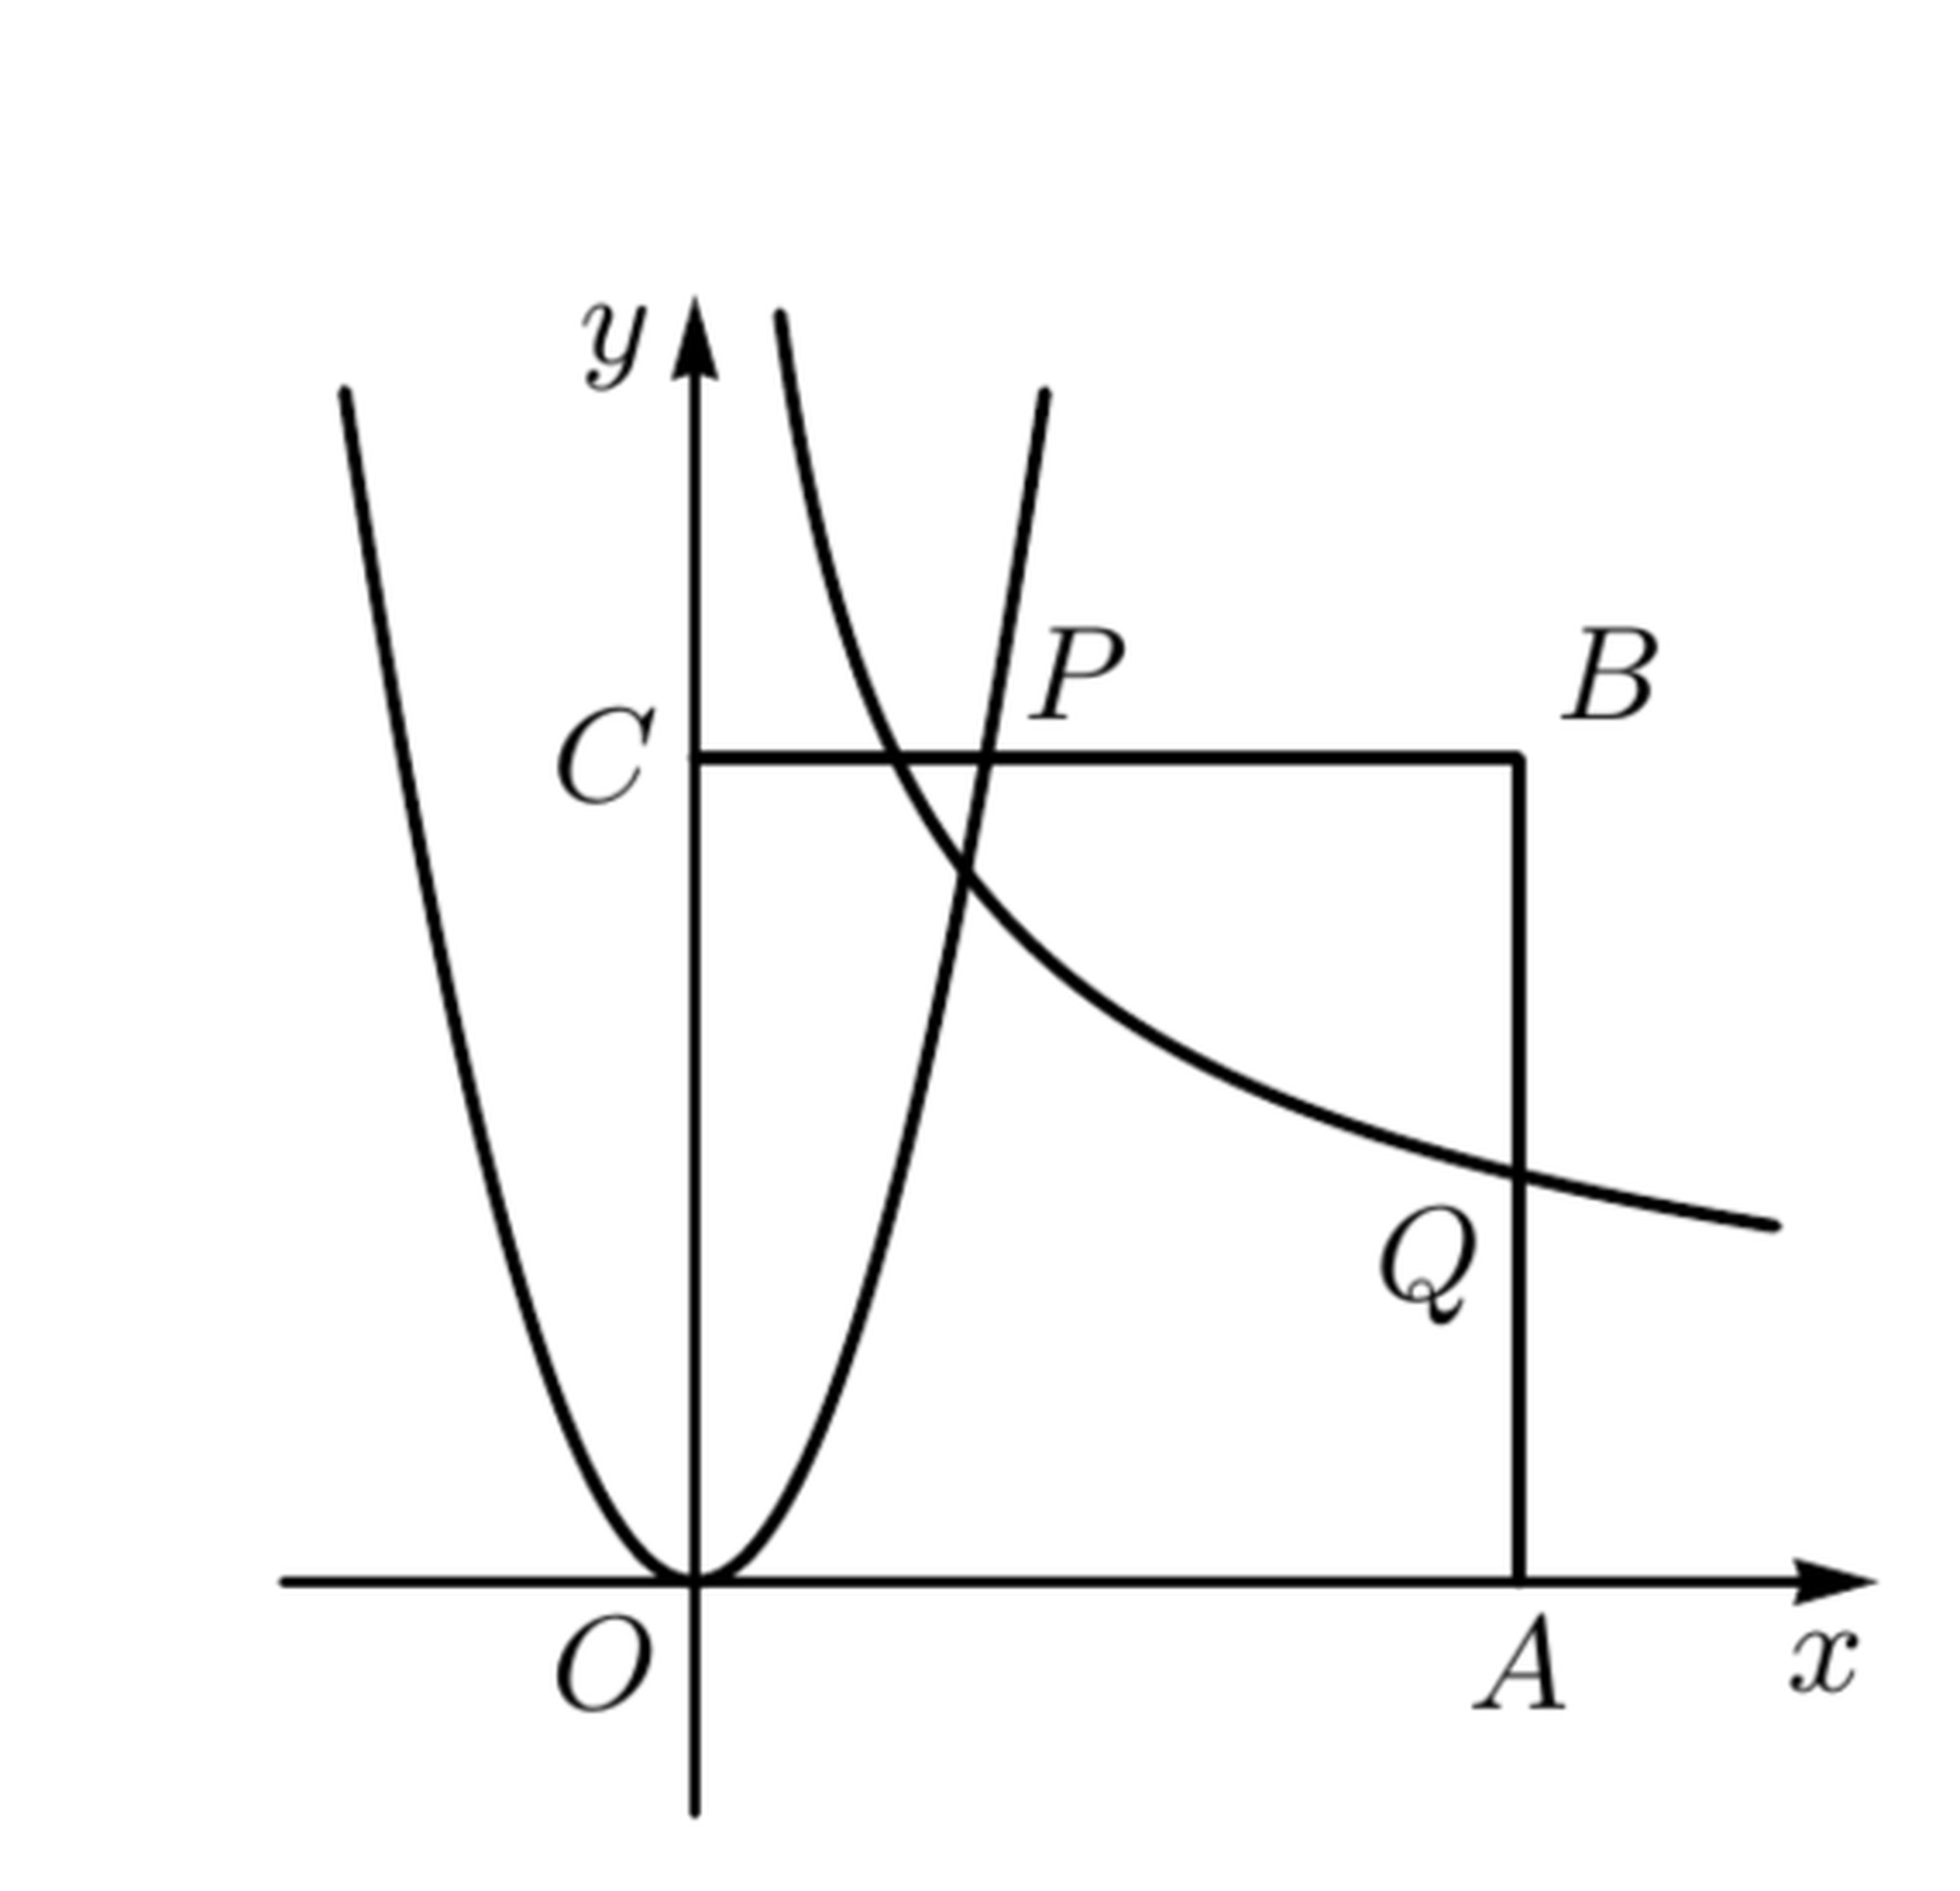
\includegraphics[width=0.40\textwidth]{figures/gao153_q11.png}
\end{center}

\ifanswer
\solbegin
\step{$\lvert AQ\rvert=\dfrac1{\sqrt a}$，$\lvert CP\rvert=\sqrt{\dfrac a5}$，}
\step{于是 $\lvert AQ\rvert+\lvert CP\rvert=\dfrac1{\sqrt a}+\sqrt{\dfrac a5}\geqslant2\sqrt{\dfrac1{\sqrt a}\cdot\sqrt{\dfrac a5}}=\dfrac2{\sqrt[4]{5}}$，}
\step{当且仅当 $\dfrac1{\sqrt a}=\sqrt{\dfrac a5}$，即 $a=\sqrt5$ 时取等号.}
\solend
\fi

% === Q12 === $B\subseteq A$ 带下划线照录、空集 \varnothing；解析 5 行
\item 若集合 $A=\{x\mid1\leqslant x\leqslant100,x\in\Z\}$，集合 $B\subseteq A$，且 $B\ne\varnothing$，记 $W(B)$ 为 $B$ 中元素的最大值与最小值之和，则对所有的 $B$，$W(B)$ 的平均值是\blankline[4.4em].

\ifanswer
\solbegin
\step{对每个非空子集 $B$，令 $B'=\{101-x\mid x\in B\}$，}
\step{则 $W(B')=(101-\min B)+(101-\max B)=202-W(B)$.}
\step{对 $B'$ 再作同样变换即得到 $B$，因此 $B$ 遍历所有非空子集时，}
\step{$B'$ 也恰好遍历所有非空子集.}
\step{设所求平均值为 $m$，则 $m=202-m$，解得 $m=101$.}
\solend
\fi

\end{enumerate}

\bigsec{二、选择题}

\begin{enumerate}
\setcounter{enumi}{12}

% === Q13 === "图像"（像，有亻）照录；解析 2 行，故选 A
\item 设 $a$、$b$ 为常数，若 $0<a<1$，$b>1$，则函数 $y=a^x-b$ 的图像必定不经过\mbox{（\quad）}

\keepwithprev
A. 第一象限\qquad\qquad B. 第二象限\qquad\qquad C. 第三象限\qquad\qquad D. 第四象限

\ifanswer
\solbegin
\step{当 $x>0$ 时，$a^x<1<b$，所以 $y=a^x-b<0$，图像必定不经过第一象限，}
\step{故选 $A$.}
\solend
\fi

% === Q14 === $m\in\Z$、中文弯引号、"图像"照录；解析 3 行，故选 A
\item 已知 $m\in\Z$，则“$m=0$”是“幂函数 $y=x^{m^2-2m-1}$ 的图像与 $x$ 轴及 $y$ 轴均无交点，且关于原点成中心对称”的\mbox{（\quad）}

\keepwithprev
A. 充分不必要条件\qquad\qquad B. 必要不充分条件

C. 充要条件\qquad\qquad D. 既不充分也不必要条件

\ifanswer
\solbegin
\step{图像满足所述条件 $\Leftrightarrow m^2-2m-1$ 为负奇数 $\Leftrightarrow m=0$ 或 $m=2$.}
\step{$m=0$ 能推出所述条件，但所述条件不能推出 $m=0$，因此是充分不必要条件，}
\step{故选 $A$.}
\solend
\fi

% === Q15 === 四选项一行；解析 5 行（跨 03→04 页），故选 D
\item 设 $a>b>1$，$x>1$，则下列不等式正确的是\mbox{（\quad）}

\keepwithprev
A. $a^x<b^x$\qquad B. $x^a<x^b$\qquad C. $\log_a x>\log_b x$\qquad D. $\log_x a>\log_x b$

\ifanswer
\solbegin
\step{$x>1$，幂函数与指数函数的单调性给出 $a^x>b^x$，$x^a>x^b$，A、B 错误.}
\step{$\log_a x=\dfrac{\lg x}{\lg a}<\dfrac{\lg x}{\lg b}=\log_b x$，C 错误.}
\step{对数函数 $y=\log_x t$ 的底数 $x>1$，在 $(0,+\infty)$ 上严格递增，}
\step{所以 $\log_x a>\log_x b$，D 正确.}
\step{故选 $D$.}
\solend
\fi

% === Q16 === $a\in\N$；解析 3 行，故选 C
\item 设 $a\in\N$，则满足不等式 $x^2-a^2x-a^2-1<0$ 的整数 $x$ 的个数不可能是\mbox{（\quad）}

\keepwithprev
A. 1\qquad\qquad B. 50\qquad\qquad C. 100\qquad\qquad D. 2026

\ifanswer
\solbegin
\step{$(x+1)(x-a^2-1)<0\Leftrightarrow-1<x<a^2+1$. 整数解为 $0,1,\cdots,a^2$，共 $a^2+1$ 个.}
\step{$1=0^2+1$，$50=7^2+1$，$2026=45^2+1$，而 $100-1=99$ 不是完全平方数，}
\step{故选 $C$.}
\solend
\fi

\end{enumerate}

\bigsec{三、解答题}

\begin{enumerate}
\setcounter{enumi}{16}

% === Q17 === 补集上划线 \overline{A}、\subseteq 照录；解析 5 行
\item 已知全集 $U=\R$，集合 $A=\{x\mid x^2-x-2\geqslant0\}$，$B=\{x\mid x>-1\}$，$C=\{x\mid a-5<x<a\}$.

(1) 求 $A\cap B$、$A\cup B$；

(2) 若 $\overline{A}\cup C=C$，求实数 $a$ 的取值范围.

\ifanswer
\solbegin
\step{(1) $x^2-x-2=(x+1)(x-2)\geqslant0\Leftrightarrow x\leqslant-1$ 或 $x\geqslant2$，}
\step{所以 $A=(-\infty,-1]\cup[2,+\infty)$，$B=(-1,+\infty)$，}
\step{因此 $A\cap B=[2,+\infty)$，$A\cup B=\R$.}
\step{(2) $\overline{A}=(-1,2)$，于是 $\overline{A}\cup C=C\Leftrightarrow\overline{A}\subseteq C\Leftrightarrow(-1,2)\subseteq(a-5,a)$，}
\step{两区间均为开区间，端点可重合，故 $\begin{cases}a-5\leqslant-1\\a\geqslant2\end{cases}\Leftrightarrow2\leqslant a\leqslant4$.}
\solend
\fi

% === Q18 === 解析 4 行
\item 已知 $a$、$b$、$c$ 都是正数，

(1) 若 $a+b=1$，求证：$\dfrac1a+\dfrac1b\geqslant4$，并指出等号成立的条件；

(2) 若 $a+b+c=1$，求证：三个数 $\dfrac1a$、$\dfrac1b$、$\dfrac1c$ 中至少有一个不小于 3.

\ifanswer
\solbegin
\step{(1) 由 $(a-b)^2\geqslant0$，得 $4ab\leqslant(a+b)^2=1$，所以 $\dfrac1a+\dfrac1b=\dfrac{a+b}{ab}=\dfrac1{ab}\geqslant4$，}
\step{等号成立当且仅当 $a=b$，结合 $a+b=1$，得 $a=b=\dfrac12$.}
\step{(2) 假设三个数 $\dfrac1a$、$\dfrac1b$、$\dfrac1c$ 都小于 3，则 $a>\dfrac13,b>\dfrac13,c>\dfrac13\Rightarrow a+b+c>1$，}
\step{与 $a+b+c=1$ 矛盾，因此三个数中至少有一个不小于 3.}
\solend
\fi

% === Q19 === 题目配图（三版都出）；\needvspace 守卫放 \item 之前；解析 19 行
\needvspace{8cm}
\item 某新建居民小区有一直角三角形绿地，两直角边长分别为 30m 和 40m，打算在其中划出一片区域改造成活动场地，如图所示.

(1) 若划出的区域为正方形，且有两边落在绿地边界上，求此正方形边长；

(2) 若划出的区域为圆形，求圆形区域面积的最大值；

(3) 若划出的区域为矩形（其中至少有一边在边界上），求此矩形面积的最大值.

\begin{center}
% 直角三角形 ABC 绿地示意图取 05 页右上，去粉色水印、去色、4× LANCZOS 放大；三版都出
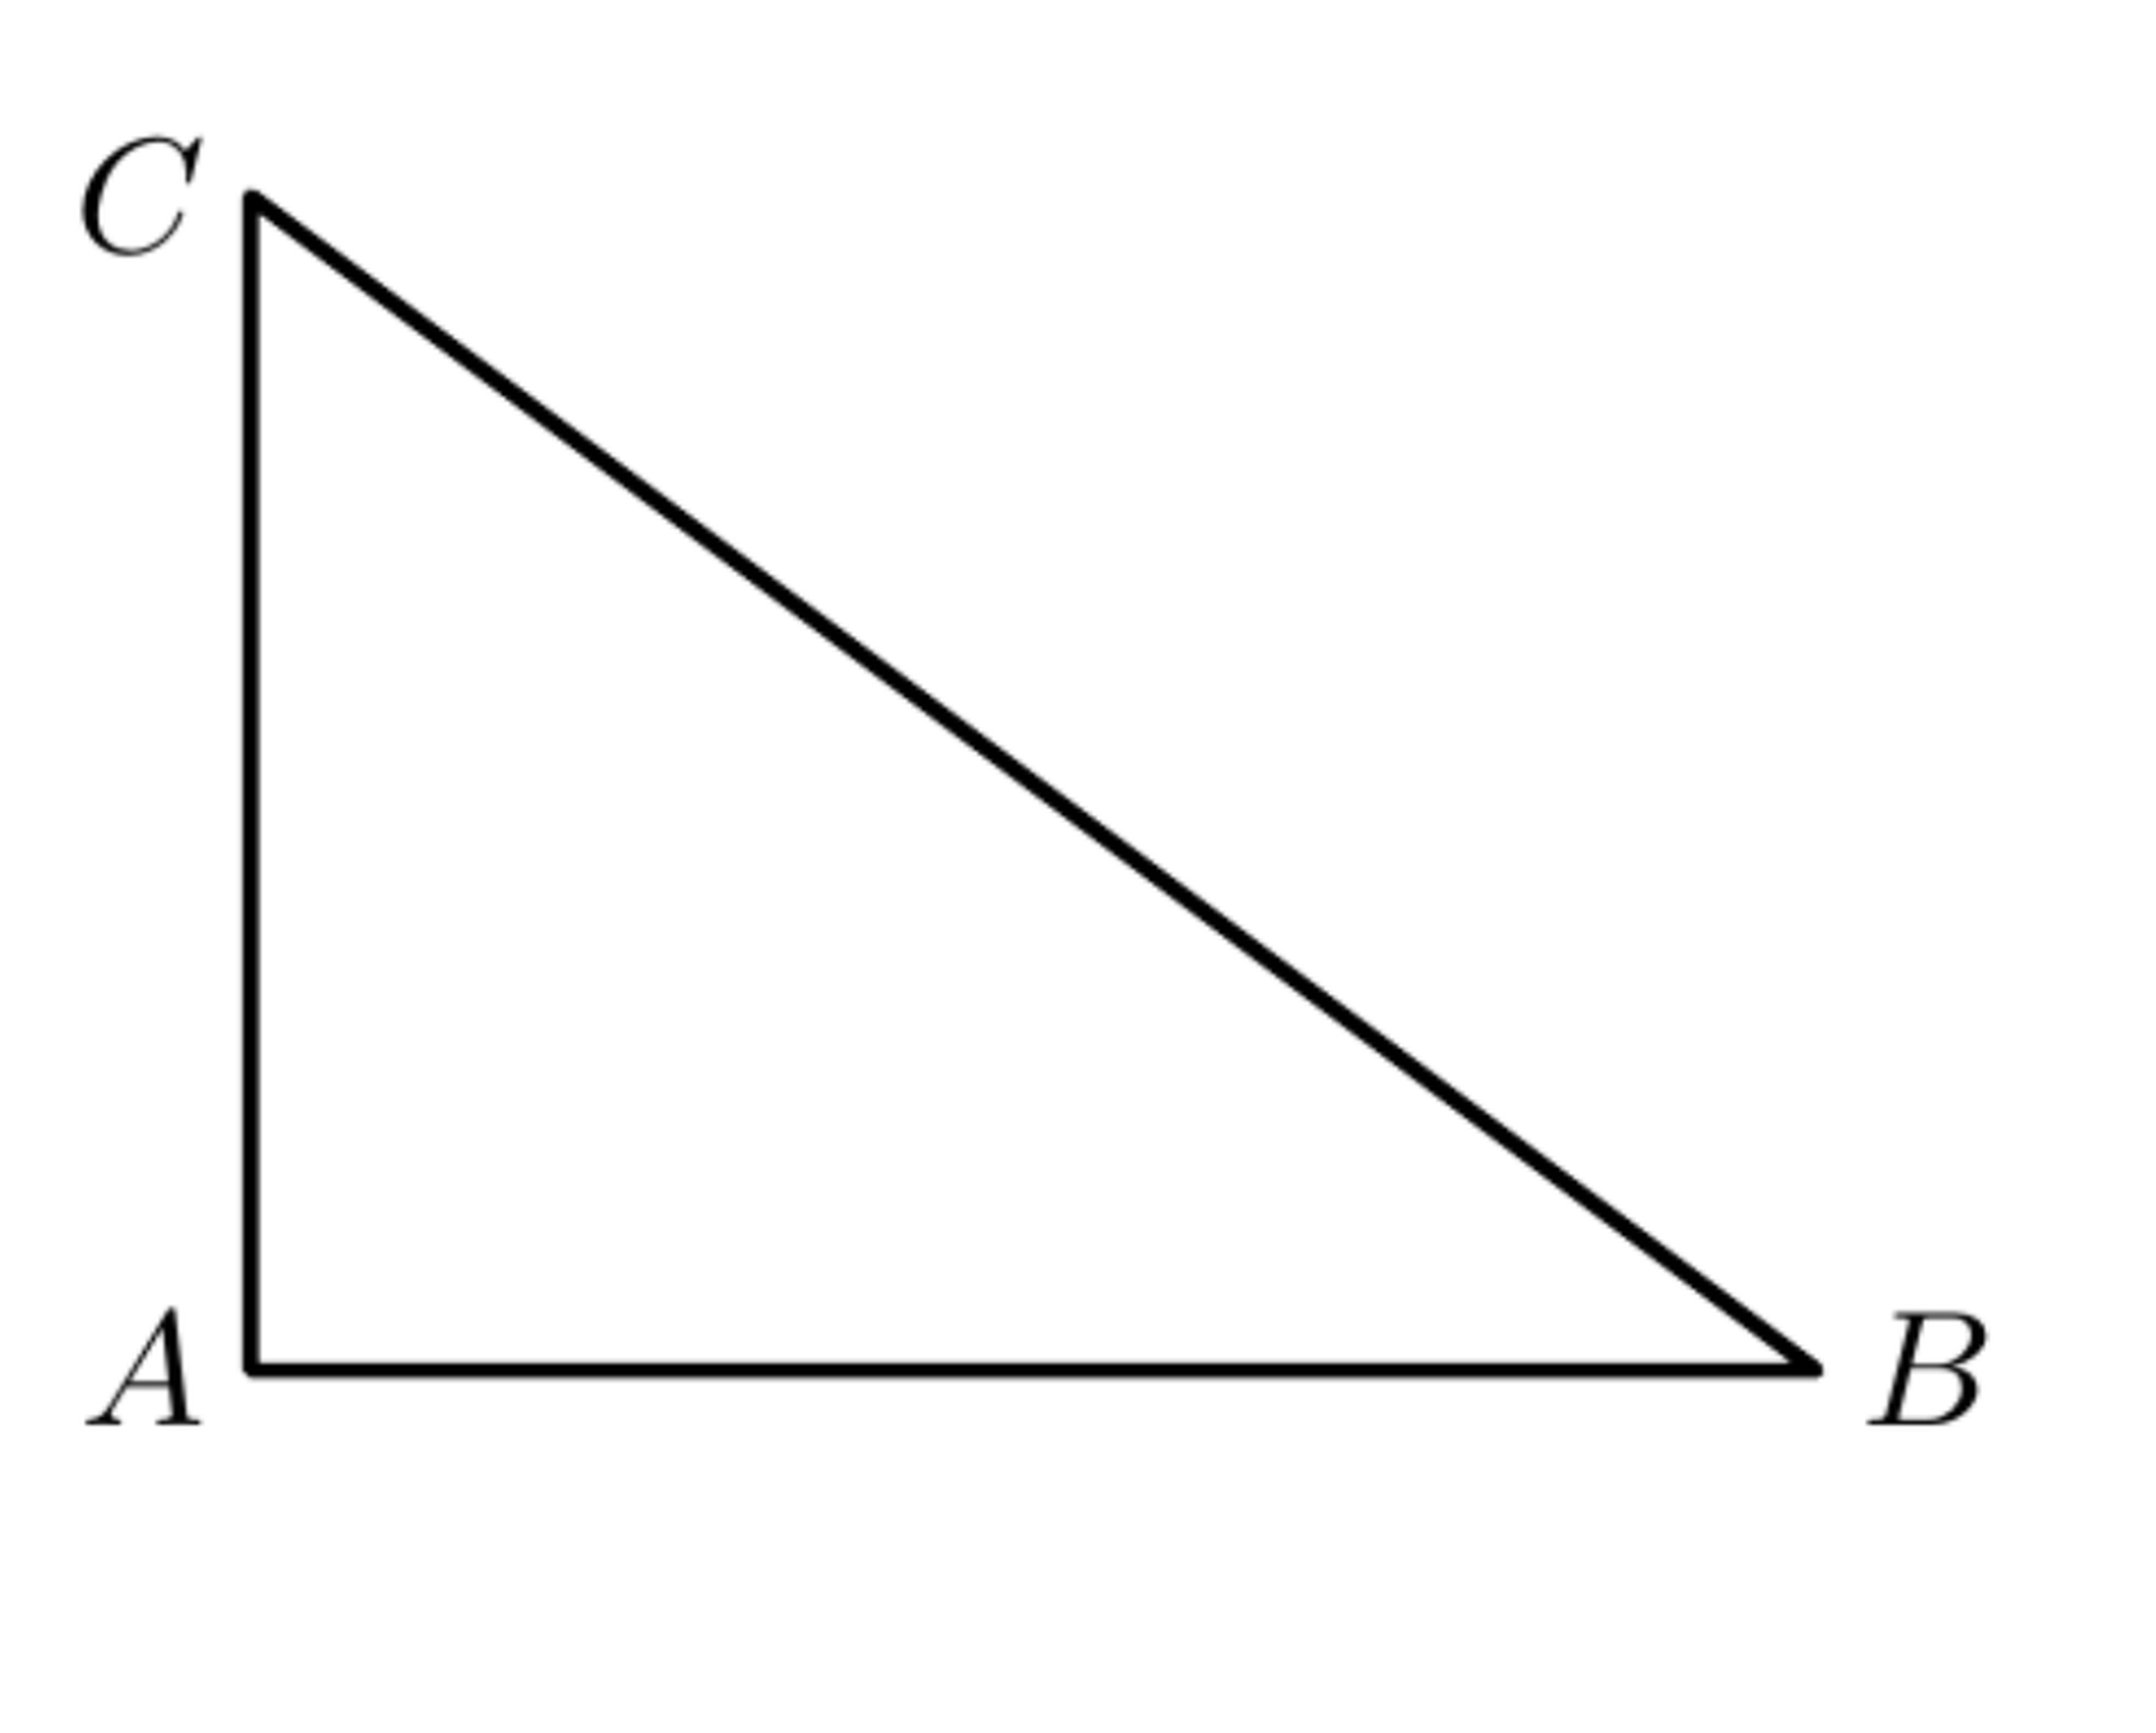
\includegraphics[width=0.34\textwidth]{figures/gao153_q19.png}
\end{center}

\ifanswer
\solbegin
\step{(1) 取 $A(0,0)$、$B(40,0)$、$C(0,30)$，则斜边 $BC$ 所在直线为 $3x+4y=120$.}
\step{正方形落在边界上的两边必分别在两条直角边上.}
\step{设其边长为 $a$m，则对角顶点为 $(a,a)$.}
\step{按题意划出的正方形应尽量大，即对角顶点落在斜边 $BC$ 上，}
\step{因此 $3a+4a=120\Rightarrow a=\dfrac{120}{7}$；}
\step{(2) 斜边长 $BC=\sqrt{30^2+40^2}=50$m，三角形面积为 $600\text{m}^2$.}
\step{设圆的半径为 $r$，圆心到 $AB$、$AC$、$BC$ 的距离分别为 $d_1,d_2,d_3$，}
\step{则三者均不小于 $r$. 连接圆心与三个顶点，}
\step{得 $600=\dfrac12(40d_1+30d_2+50d_3)\geqslant\dfrac12(40+30+50)r=60r$，所以 $r\leqslant10$.}
\step{取三角形的内切圆时等号成立，圆形区域面积的最大值为 $100\pi\text{m}^2$.}
\step{(3) 任取矩形落在绿地边界上的一边，以其所在直线为横轴.}
\step{设相应三角形底边长为 $L$、高为 $H$，则 $LH=1200$.}
\step{取三角形顶点坐标为 $(0,0)$、$(L,0)$、$(p,H)$.}
\step{在高度 $t$ 处，两腰上的点的横坐标分别为 $\dfrac{pt}{H}$、$L+\dfrac{(p-L)t}{H}$，}
\step{因此，高为 $t$ 的矩形，其底边长不超过 $L\left(1-\dfrac tH\right)$，}
\step{面积满足 $S\leqslant Lt\left(1-\dfrac tH\right)=\dfrac LH\left[\dfrac{H^2}{4}-\left(t-\dfrac H2\right)^2\right]\leqslant\dfrac{LH}{4}=300$，}
\step{在原坐标系中，取矩形顶点为 $(0,0)$、$(20,0)$、$(20,15)$、$(0,15)$，}
\step{其中 $3\times20+4\times15=120$，矩形完全位于绿地内，面积为 $300\text{m}^2$，}
\step{达到最大值.}
\solend
\fi

% === Q20 === $g(x)$ 定义照录；解析 14 行
\item 已知 $a>0$ 且 $a\ne1$，设 $f(x)=\log_a(x^2-a^2)$，$g(x)=2\log_a(x-ak)$.

(1) 求函数 $y=f(x)$ 的定义域；

(2) 若 $k=2$，求不等式 $f(x)>g(x)$ 的解集；

(3) 若“存在实数 $x$，使得 $f(x)=g(x)$”为真命题，求实数 $k$ 的取值范围.

\ifanswer
\solbegin
\step{(1) $x^2-a^2>0\Leftrightarrow x<-a$ 或 $x>a$，定义域为 $(-\infty,-a)\cup(a,+\infty)$.}
\step{(2) 两函数均有意义时，$x>2a$，且 $g(x)=\log_a(x-2a)^2$.}
\step{当 $a>1$ 时，$f(x)>g(x)\Leftrightarrow x^2-a^2>(x-2a)^2\Leftrightarrow x>\dfrac{5a}{4}$，}
\step{结合 $x>2a$，解集为 $(2a,+\infty)$.}
\step{当 $0<a<1$ 时，$f(x)>g(x)\Leftrightarrow x^2-a^2<(x-2a)^2\Leftrightarrow x<\dfrac{5a}{4}$，}
\step{与 $x>2a$ 矛盾，解集为 $\varnothing$.}
\step{(3) 在 $x^2-a^2>0$ 且 $x-ak>0$ 的条件下，}
\step{$f(x)=g(x)\Leftrightarrow x^2-a^2=(x-ak)^2\Leftrightarrow2akx=a^2(1+k^2)$，}
\step{当 $k=0$ 时，上式不成立；}
\step{当 $k\ne0$ 时，$x=\dfrac{a(1+k^2)}{2k}$，}
\step{于是 $x-ak=\dfrac{a(1-k^2)}{2k}>0\Leftrightarrow k<-1$ 或 $0<k<1$，}
\step{对上述 $k$，所取的 $x$ 同时满足 $x^2-a^2=(x-ak)^2>0$，}
\step{两函数均有意义且函数值相等.}
\step{因此，$k$ 的取值范围为 $(-\infty,-1)\cup(0,1)$.}
\solend
\fi

% === Q21 === 中文弯引号、复杂式照录；解析 23 行（跨 08→09 页）
\item 若实数 $x$、$y$、$m$ 满足 $\lvert x-m\rvert<\lvert y-m\rvert$，则称 $x$ 比 $y$ 接近 $m$.

(1) 若 $2x$ 比 $x-2$ 更接近 1，求实数 $x$ 的取值范围；

(2) 若 $x$ 比 $y$ 接近 $m$，证明：“$x>y$” 的充要条件是 “$x+y<2m$”；

(3) 已知 $x>0$，$y>0$ 且 $x\ne y$. 设 $p=\dfrac{x^2+y^2}{xy}$，若对于任意的 $x$、$y$，命题 “$p$ 比 $p^2-3p+4$ 接近 $m$” 恒成立，求实数 $m$ 的取值范围.

\ifanswer
\solbegin
\step{(1) $\lvert2x-1\rvert<\lvert x-3\rvert\Leftrightarrow(2x-1)^2<(x-3)^2\Leftrightarrow(x+2)(3x-4)<0$，}
\step{解得 $-2<x<\dfrac43$，实数 $x$ 的取值范围为 $\left(-2,\dfrac43\right)$.}
\step{(2) 因为 $x$ 比 $y$ 接近 $m$，所以 $\lvert x-m\rvert<\lvert y-m\rvert$，则 $\lvert x-m\rvert^2<\lvert y-m\rvert^2$，}
\step{即 $(x-m)^2<(y-m)^2$，即 $(x-m)^2-(y-m)^2<0$，}
\step{即得 $(x-y)(x+y-2m)<0$，}
\step{则由 $x+y<2m$，得 $x+y-2m<0$，}
\step{故 $x-y>0$，即 $x>y$，充分性成立；}
\step{当 $x>y$ 时，$x-y>0$，结合 $(x-y)(x+y-2m)<0$，得 $x+y-2m<0$，}
\step{即 $x+y<2m$，必要性成立；}
\step{故“$x>y$” 的充要条件是 “$x+y<2m$”；}
\step{(3) $x>0$，$y>0$ 且 $x\ne y$. 则 $p=\dfrac{x^2+y^2}{xy}=\dfrac xy+\dfrac yx>2\sqrt{\dfrac xy\cdot\dfrac yx}=2$，}
\step{由于对于任意的 $x$、$y$，命题 “$p$ 比 $p^2-3p+4$ 接近 $m$” 恒成立，}
\step{故 $\lvert p-m\rvert<\lvert(p^2-3p+4)-m\rvert$ 对 $\forall p>2$ 恒成立，}
\step{即得 $(p-m)^2<(p^2-3p+4-m)^2$，}
\step{即 $(p^2-3p+4-m)^2-(p-m)^2>0$，}
\step{得 $(p^2-4p+4)(p^2-2p+4-2m)>0$，}
\step{即 $(p-2)^2(p^2-2p+4-2m)>0$，由于 $p>2$，故 $(p-2)^2>0$，}
\step{故 $p^2-2p+4-2m>0$ 对 $\forall p>2$ 恒成立，}
\step{即 $2m<p^2-2p+4$ 对 $\forall p>2$ 恒成立，}
\step{由于 $p^2-2p+4=(p-1)^2+3$，此时 $p^2-2p+4$ 在 $(2,+\infty)$ 上严格增，}
\step{故 $(p-1)^2+3>(2-1)^2+3=4$，故 $2m\leqslant4$，解得 $m\leqslant2$，}
\step{即实数 $m$ 的取值范围是 $(-\infty,2]$.}
\solend
\fi

\end{enumerate}

\end{document}
"
% 紧凑版：xelatex "\def\iscompact{1}% 高一153_闵行中学文绮中学_期中.tex
%   —— 高一上数学"2026-2027 年闵行中学文绮中学高一上期中"（试卷版/答案版/紧凑版）
% 试卷版：xelatex 高一153_闵行中学文绮中学_期中.tex
% 答案版：xelatex "\def\isanswer{1}\input{高一153_闵行中学文绮中学_期中.tex}"
% 紧凑版：xelatex "\def\iscompact{1}\input{高一153_闵行中学文绮中学_期中.tex}"
%
% ① 原始材料：微信公众号"魔都数学加油站"文章，连载"27学年高一153"，原文标题
% "27学年高一153——2026-2027年上海市闵行中学文绮中学高一上期中"；
% 原文链接：https://mp.weixin.qq.com/s/rEtS-92cDR6JKgY2b5DRfg 。
% 正文为 9 张 PNG 页（01/02/06/07/08/09 为 2560×3620，03/04/05 为 4762×6735，
% 同一篇各页分辨率混排，逐页按各自分辨率裁图核对，别按预览比例换算裁框）。
% 体例：讲评版——填空 3—12（10 题）、选择 13—16（4 题）、解答 17—21（5 题），
% 共 19 题，自第 3 题起编；**全 19 题均印【解析】**（逐题核实，见 ② ②）。
% 题目、答案、解析均据原图转录；卷面粉红色水印"魔都数学加油站"及公众号页脚未录入。
% 全卷插图清单（逐页通读 9 页确认）：2 幅，均为题目配图、三版都出——
%   · Q11 正方形 OABC 曲线图（02 页右下：$y=5x^2$ 与 $y=x^{-\frac12}$ 两条曲线、
%     坐标轴、O/A/B/C/P/Q、正方形），裁 figures/gao153_q11.png；
%   · Q19 直角三角形 ABC 绿地示意图（05 页右上，直角在 A），
%     裁 figures/gao153_q19.png；
%   两图均去粉色水印、去色、4× LANCZOS 放大；Q11 图左上角题干残字"函"已裁白。
%   其余各页逐页确认无其它题目配图、无解析内配图、无表格；09 页下半仅水印、无正文。
%
% 卷首标题：原卷印作"2026-2027 年闵行中学文绮中学高一上期中"，年份区间按全稿惯例排 en dash；
% 原卷卷面未印副标题，本稿按同期中卷知识模块口径补出"集合与常用逻辑用语、不等式、函数"。
%
% ② 与原卷的排版差异：
%   ① 原文从第 3 题起，本稿保留原题号；共 19 题三节，解答题 5 题到 21；
%   ② 全 19 题均印【解析】、用 \solbegin…\solend，无只印【答案】或答案印括号内的题；
%      四道选择题答案在解析末句"故选 A／A／D／C"（Q13—Q16，逐个放大复核）、
%      括号 \mbox{（\quad）} 留空、不另提 \ans{}；答案版【答案】/【解析】标记数
%      = 19 = 全卷题数；
%   ③ 原卷卷面未印副标题，本稿按知识模块口径补出；
%   ④ 原卷填空横线按全稿惯例排 \blankline[4.4em]；选择题括号排 \mbox{（\quad）}、
%      四道选择题的选项段前按惯例各加 \keepwithprev；解答题不留作答区、不加
%      \anspace（原卷为讲评版，109—113 起全稿不用 \anspace）；
%   ⑤ 数集：Q3"$x\in R$"、Q5"解集为 R"、Q10"$x\in N$"、Q12"$x\in Z$"与
%      "$m\in Z$"、Q14"$m\in Z$"、Q16"$a\in N$"、Q17"全集 $U=R$"、
%      Q19 无、Q21 无——原卷印斜体或正体粗体 R/N/Z，按全稿惯例归一
%      \R／\N／\Z；绝对值排 \lvert…\rvert（Q5、Q11、Q21），集合描述竖线排 \mid
%      （Q3、Q10、Q17、Q20），不等号按全稿惯例排 \leqslant／\geqslant；
%      补集照原卷上划线排 \overline{A}（Q17 题干 (2)＋解析 (2)）；
%      空集 \varnothing（Q12 题干、Q20 解析 (2)）；子集 3 处均印带下划线 ⊆、
%      照录 \subseteq（Q10 $A\subseteq U$、Q12 $B\subseteq A$、Q17 $(-1,2)\subseteq(a-5,a)$），
%      本卷无单线 \subset 用例；
%   ⑥ 判别式：逐页通读 9 页，本卷无一元二次判别式 Δ/△ 算式，故无 Δ/△ 混用可照录；
%      Q11 图里有几何正方形 OABC（非三角形符号），无 △ABC 用例；
%   ⑦ 中文弯引号照录：Q14"$m=0$"与"幂函数…关于原点成中心对称"、
%      Q20"存在实数 $x$，使得 $f(x)=g(x)$"、Q21"$x>y$"与"$x+y<2m$"、
%      "$p$ 比 $p^2-3p+4$ 接近 $m$"（引号外留空格按原卷）；
%      注释里一律 ASCII 引号；数学式内 CJK 用 \text{}；
%   ⑧ "图像／图象"逐处放大核：全卷 3 处均印"图像"（像，有亻）——
%      Q13 题干与解析、Q14 题干与解析；Q19 题干写"如图所示"（非"图像"），
%      逐处照录未统一；子题标号 (1)(2)(3) 半角括号照录；圈数字本卷无用例；
%   ⑨ 半角逗号在数学组之间是全稿惯例、非笔误，逐处照录（Q3 $x\in R$、
%      Q10 $a_1,a_2$、Q19 $A(0,0)$、$d_1,d_2,d_3$、Q21 $a>\frac13,b>\frac13$ 等）；
%      行末西文句点 ASCII `.`；行中全角逗号／顿号照录（Q19"30m 和 40m"、
%      Q21"实数 $x$、$y$、$m$"）；
%   ⑩ 复杂式照录别简化：Q3 $y=x^{-2}$、Q11 $y=x^{-\frac12}$ 与
%      $\frac{2}{\sqrt[4]{5}}$、Q8 $\frac{2b}{a+1-b}$、Q9 cases 块、
%      Q10 $525=5\times105$、Q16 $a^2+1$、Q19 $S\leqslant Lt(1-\frac tH)$
%      与 $L+\frac{(p-L)t}{H}$、Q20 $2akx=a^2(1+k^2)$ 与 $\frac{a(1+k^2)}{2k}$、
%      Q21 $(p^2-4p+4)(p^2-2p+4-2m)>0$；
%      \left…\right 不得拆到不同 $…$ 组（Q17 $\left\{x\mid\cdots\right\}$、
%      Q19 $\left[\frac{H^2}{4}-\left(t-\frac H2\right)^2\right]$、
%      Q21 $\left(-2,\frac43\right)$ 等）；cases 块一律 \begin{cases}…\end{cases}；
%   ⑪ 一条 \step = 原卷解析的一个印刷行，cases 块整体算一个印刷行；别并折行、
%      别拆行。Q10 六行、Q19 十九行、Q20 十四行、Q21 二十二行均按印刷行逐条断，
%      不丢行；
%   ⑫ 配图：Q11／Q19 题目配图（三版都出）放 \item 内题干之后 \begin{center}，
%      各用 \needvspace{8cm} 守卫把整块推走，**守卫放在 \item 之前**
%      （见 高一145 Q14/Q20 成例与切页审计 B 类坑）；
%   ⑬ 原卷解析内无红色"法一／法二"之类小标题，故本卷无 \stepm；红色水印
%      "魔都数学加油站"不录入；
%   ⑭ 跨页续印按题合并：见 ⑥；
%
% ③ 行数复核：一条 \step = 原卷解析的一个印刷行，cases 块作一个印刷行计。
%   逐题数（主会话逐页核对定稿）：Q3：1；Q4：2；Q5：2；Q6：2；Q7：1；
%   Q8：1；Q9：2；Q10：6；Q11：3；Q12：5；Q13：2；Q14：3；Q15：5；
%   Q16：3；Q17：5；Q18：4；Q19：19；Q20：14；Q21：22。
%   合计 102 条 \step（本卷无 \stepm），与原卷逐题印刷行相等。全卷 19 题
%   均设 \solbegin…\solend，答案版【答案】/【解析】标记数 = 19 = 全卷题数。
%
% ④ 判别式／子集符号结论（逐处放大原图照录、不得统一，主会话像素级复核）：
%   判别式：逐页通读 9 页，本卷无一元二次判别式算式（Q7 用韦达定理、
%      Q16 用因式分解、Q20 用对数方程，均不写 Δ/△），故无 Δ/△ 混用可照录
%      （"高 \Delta／扁 \triangle"口径备查，参照 高一142／151／152 头注）；
%      本卷无几何三角形符号用例。
%   子集：Q10 题干"$A\subseteq U$"、Q12 题干"$B\subseteq A$"、Q17 解析 (2)
%      "$(-1,2)\subseteq(a-5,a)$"共 3 处，逐处放大确认均印带下划线 ⊆、
%      照录 \subseteq；本卷未见单线 ⊂（\subset）之对应处。
%      补集上划线 \overline{A}（Q17）、空集 \varnothing（Q12 题干、Q20 解析 (2)）；
%      数集 \R／\N／\Z 归一见 ② ⑤。
%
% ⑤ 存疑照录（放大原图确认，照录未改、正文对应处另有 % 注）：
%   1. Q3 集合 $B=\{(x,y)\mid y=x^{-2},x\in\R\}$ 原卷题干径写 $x\in\R$
%      （$x=0$ 处无意义），解析自行注明 $x\ne0$，照录未改。
%   2. Q10 解析"$U$ 中共有 $525=5\times105$ 个连续整数"与尾行
%      "取 $U$ 中除以 5 余 1 或 2 的全部元素及元素 5"逐字照录（放大 02 页
%      /tmp/gao153/z/zoom/q10_pick.png 确认是"元素 5"，非"元素 9"）。
%   3. Q11 第二个函数原卷印 $y=x^{-\frac12}$（负二分之一次幂，非 $x^2$），
%      放大 02 页 /tmp/gao153/z/zoom/q11_exp.png 确认，照录未改；
%      $|AQ|=\frac1{\sqrt a}$ 与之自洽。
%   4. Q19 (3) 解析"在高度 $t$ 处，两腰上的点的横坐标分别为 $\frac{pt}{H}$、
%      $L+\frac{(p-L)t}{H}$"，放大 06 页确认，照录未简化。
%   5. Q20 (2) 解析"$g(x)=\log_a(x-2a)^2$"（真数整体平方），
%      与 $g(x)=2\log_a(x-ak)$ 在 $k=2$ 时一致，照录未改。
%   6. Q21 (3) 解析"得 $(p^2-4p+4)(p^2-2p+4-2m)>0$"与
%      "故 $(p-1)^2+3>(2-1)^2+3=4$，故 $2m\leqslant4$"照录未改
%      （放大 09 页 /tmp/gao153/z/zoom/q21_factor.png 确认）。
%   7. "图像／图象"全卷 3 处均印"图像"（像，有亻）逐处照录；
%      本卷无判别式 Δ/△ 用例（见 ④）。
%   全卷除此 7 类外未发现其它笔误／自相矛盾处；19 题均印【解析】、
%   无只印【答案】或答案印括号内的题（见 ② ②）。
%
% ⑥ 跨页续印按题合并说明（逐页核实定稿）：Q3—Q5 题干＋解析在 01 页；
%   Q6—Q8 题干＋解析在 01 页下半（Q8 解析续 02 页顶）；Q9 题干＋解析、
%   Q10 题干＋解析首 2 行在 02 页上半，Q10 解析余 4 行在 02 页下半；
%   Q11 题干＋配图＋解析、Q12 题干＋解析 5 行在 02 页下半—03 页上半；
%   "二、选择题"标题在 03 页中部；Q13 题干＋选项＋解析在 03 页下半；
%   Q14 题干＋选项＋解析、Q15 题干＋选项＋解析首行在 03 页下半—04 页顶；
%   Q15 解析余 4 行、Q16 题干＋选项＋解析在 04 页上半；"三、解答题"
%   标题在 04 页下半；Q17 题干＋两问＋解析 5 行在 04 页下半—05 页顶；
%   Q18 题干＋两问＋解析 4 行、Q19 题干（含配图）＋三问在 05 页；
%   Q19 解析 (1)(2) 9 行在 05 页下半，解析 (3) 前 5 行在 06 页上半、
%   余 4 行在 06 页下半；Q20 题干＋三问在 06 页下半，解析 (1)(2)(3)
%   前 6 行在 07 页上半、(3) 余 8 行在 07 页下半；Q21 题干＋三问在
%   07 页末，解析 (1)(2) 10 行在 08 页上半—下半，解析 (3) 前 4 行在
%   08 页下半、余 9 行续 09 页上半，末行"即实数 $m$ 的取值范围是
%   $(-\infty,2]$"为全卷收尾（09 页下半仅水印、无正文）。
%   本稿按题连排，不丢行、不并折行；全卷末题为第 21 题，无附加题节。
%
\documentclass[a4paper,11pt]{article}
\usepackage{common}

\begin{document}

\examtitlest[3]{2026--2027 年闵行中学文绮中学高一上期中}{集合与常用逻辑用语、不等式、函数}

\bigsec{一、填空题}

\begin{enumerate}
\setcounter{enumi}{2}

% === Q3 === 集合描述竖线 \mid；$y=x^{-2}$ 照录；解析 1 行
\item 已知 $A=\{(x,y)\mid y=x^3,x\in\R\}$，$B=\{(x,y)\mid y=x^{-2},x\in\R\}$，则 $A\cap B=$\blankline[4.4em].

\ifanswer
\solbegin
\step{$x^3=x^{-2}\ (x\ne0)\Leftrightarrow x^5=1\Leftrightarrow x=1$，此时 $y=1$，所以 $A\cap B=\{(1,1)\}$.}
\solend
\fi

% === Q4 === 解析 2 行
\item 若关于 $x$ 的不等式 $\dfrac{x-a}{x+1}>0$ 的解集为 $(-\infty,-1)\cup(4,+\infty)$，则实数 $a=$\blankline[4.4em].

\ifanswer
\solbegin
\step{关于 $x$ 的不等式 $\dfrac{x-a}{x+1}>0$ 即 $(x+1)(x-a)>0$.}
\step{再由它的解集为 $(-\infty,-1)\cup(4,+\infty)$，得 $-1$ 和 4 是 $(x+1)(x-a)=0$ 的两个实数根，故 $a=4$.}
\solend
\fi

% === Q5 === 绝对值 \lvert…\rvert；解析 2 行
\item 若关于 $x$ 的不等式 $\lvert x+1\rvert+\lvert x-2\rvert>m$ 的解集为 $\R$，则实数 $m$ 的取值范围是\blankline[4.4em].

\ifanswer
\solbegin
\step{$\lvert x+1\rvert+\lvert x-2\rvert\geqslant\lvert(x+1)-(x-2)\rvert=3$，当且仅当 $-1\leqslant x\leqslant2$ 时取等号，}
\step{因此 $m<3$.}
\solend
\fi

% === Q6 === 解析 2 行
\item 已知指数函数 $y=a^x$（$a>1$）在区间 $[-1,1]$ 上的最大值比最小值大 $\dfrac32$，则实数 $a=$\blankline[4.4em].

\ifanswer
\solbegin
\step{$a>1$，指数函数在 $[-1,1]$ 上严格增，故 $a-\dfrac1a=\dfrac32\Leftrightarrow(a-2)(2a+1)=0$.}
\step{结合 $a>1$，得 $a=2$.}
\solend
\fi

% === Q7 === 韦达定理；解析 1 行
\item 已知关于 $x$ 的一元二次方程 $x^2+px+2p=0$ 的两个实数根分别为 $x_1$、$x_2$，且 $(x_1+1)(x_2+1)=0$，则 $p=$\blankline[4.4em].

\ifanswer
\solbegin
\step{$0=(x_1+1)(x_2+1)=x_1x_2+x_1+x_2+1=2p-p+1=p+1\Rightarrow p=-1$.}
\solend
\fi

% === Q8 === 换底公式；解析 1 行
\item 已知 $10^a=3$，$\lg5=b$，则 $\log_6 25=$\blankline[4.4em]（用关于 $a,b$ 的关系式表示）.

\ifanswer
\solbegin
\step{$\lg3=a$，$\lg2=1-b$，所以 $\log_6 25=\dfrac{\lg25}{\lg6}=\dfrac{2b}{a+1-b}$.}
\solend
\fi

% === Q9 === cases 块整体算一个印刷行；解析 2 行
\item 已知 $A=[2,5]$，若对任意 $x\in A$，总有 $\dfrac{k}{x}\in A$，则正数 $k=$\blankline[4.4em].

\ifanswer
\solbegin
\step{$k>0$，当 $x\in[2,5]$ 时，$\dfrac{k}{x}$ 的取值范围为 $\left[\dfrac k5,\dfrac k2\right]$，}
\step{因此 $\begin{cases}\dfrac k5\geqslant2\\\dfrac k2\leqslant5\end{cases}\Leftrightarrow10\leqslant k\leqslant10\Leftrightarrow k=10$.}
\solend
\fi

% === Q10 === $A\subseteq U$ 带下划线照录；解析 6 行
\item 已知集合 $U=\{x\mid4\leqslant x\leqslant528,x\in\N\}$，$A=\{a_1,a_2,a_3,\cdots,a_n\}$，且 $A\subseteq U$. 如果集合 $A$ 中的任意两个不同元素之和都不能被 5 整除，则正整数 $n$ 的最大值为\blankline[4.4em].

\ifanswer
\solbegin
\step{$U$ 中共有 $525=5\times105$ 个连续整数，按除以 5 的余数分成五类，}
\step{每类均有 105 个元素.}
\step{余数为 1,4 的两类不能同时选取，余数为 2,3 的两类也不能同时选取，}
\step{余数为 0 的一类最多选 1 个，因此 $n\leqslant105+105+1=211$.}
\step{取 $U$ 中除以 5 余 1 或 2 的全部元素及元素 5，}% 放大 02 页确认是「元素 5」（非 9），照录未改（见 ⑤ 2）
\step{任意两个不同元素之和均不能被 5 整除，此时 $n=211$，最大值为 211.}
\solend
\fi

% === Q11 === 题目配图（三版都出）；\needvspace 守卫放 \item 之前；$y=x^{-\frac12}$ 照录；解析 3 行
\needvspace{8cm}
\item 如图，已知正方形 $OABC$，其中 $OA=a$（$a>1$），函数 $y=5x^2$ 交 $BC$ 于点 $P$，函数 $y=x^{-\frac12}$ 交 $AB$ 于点 $Q$，当 $\lvert AQ\rvert+\lvert CP\rvert$ 最小时，$a$ 的值为\blankline[4.4em].

\begin{center}
% 正方形 OABC 与两条曲线图取 02 页右下，去粉色水印、去色、4× LANCZOS 放大；三版都出
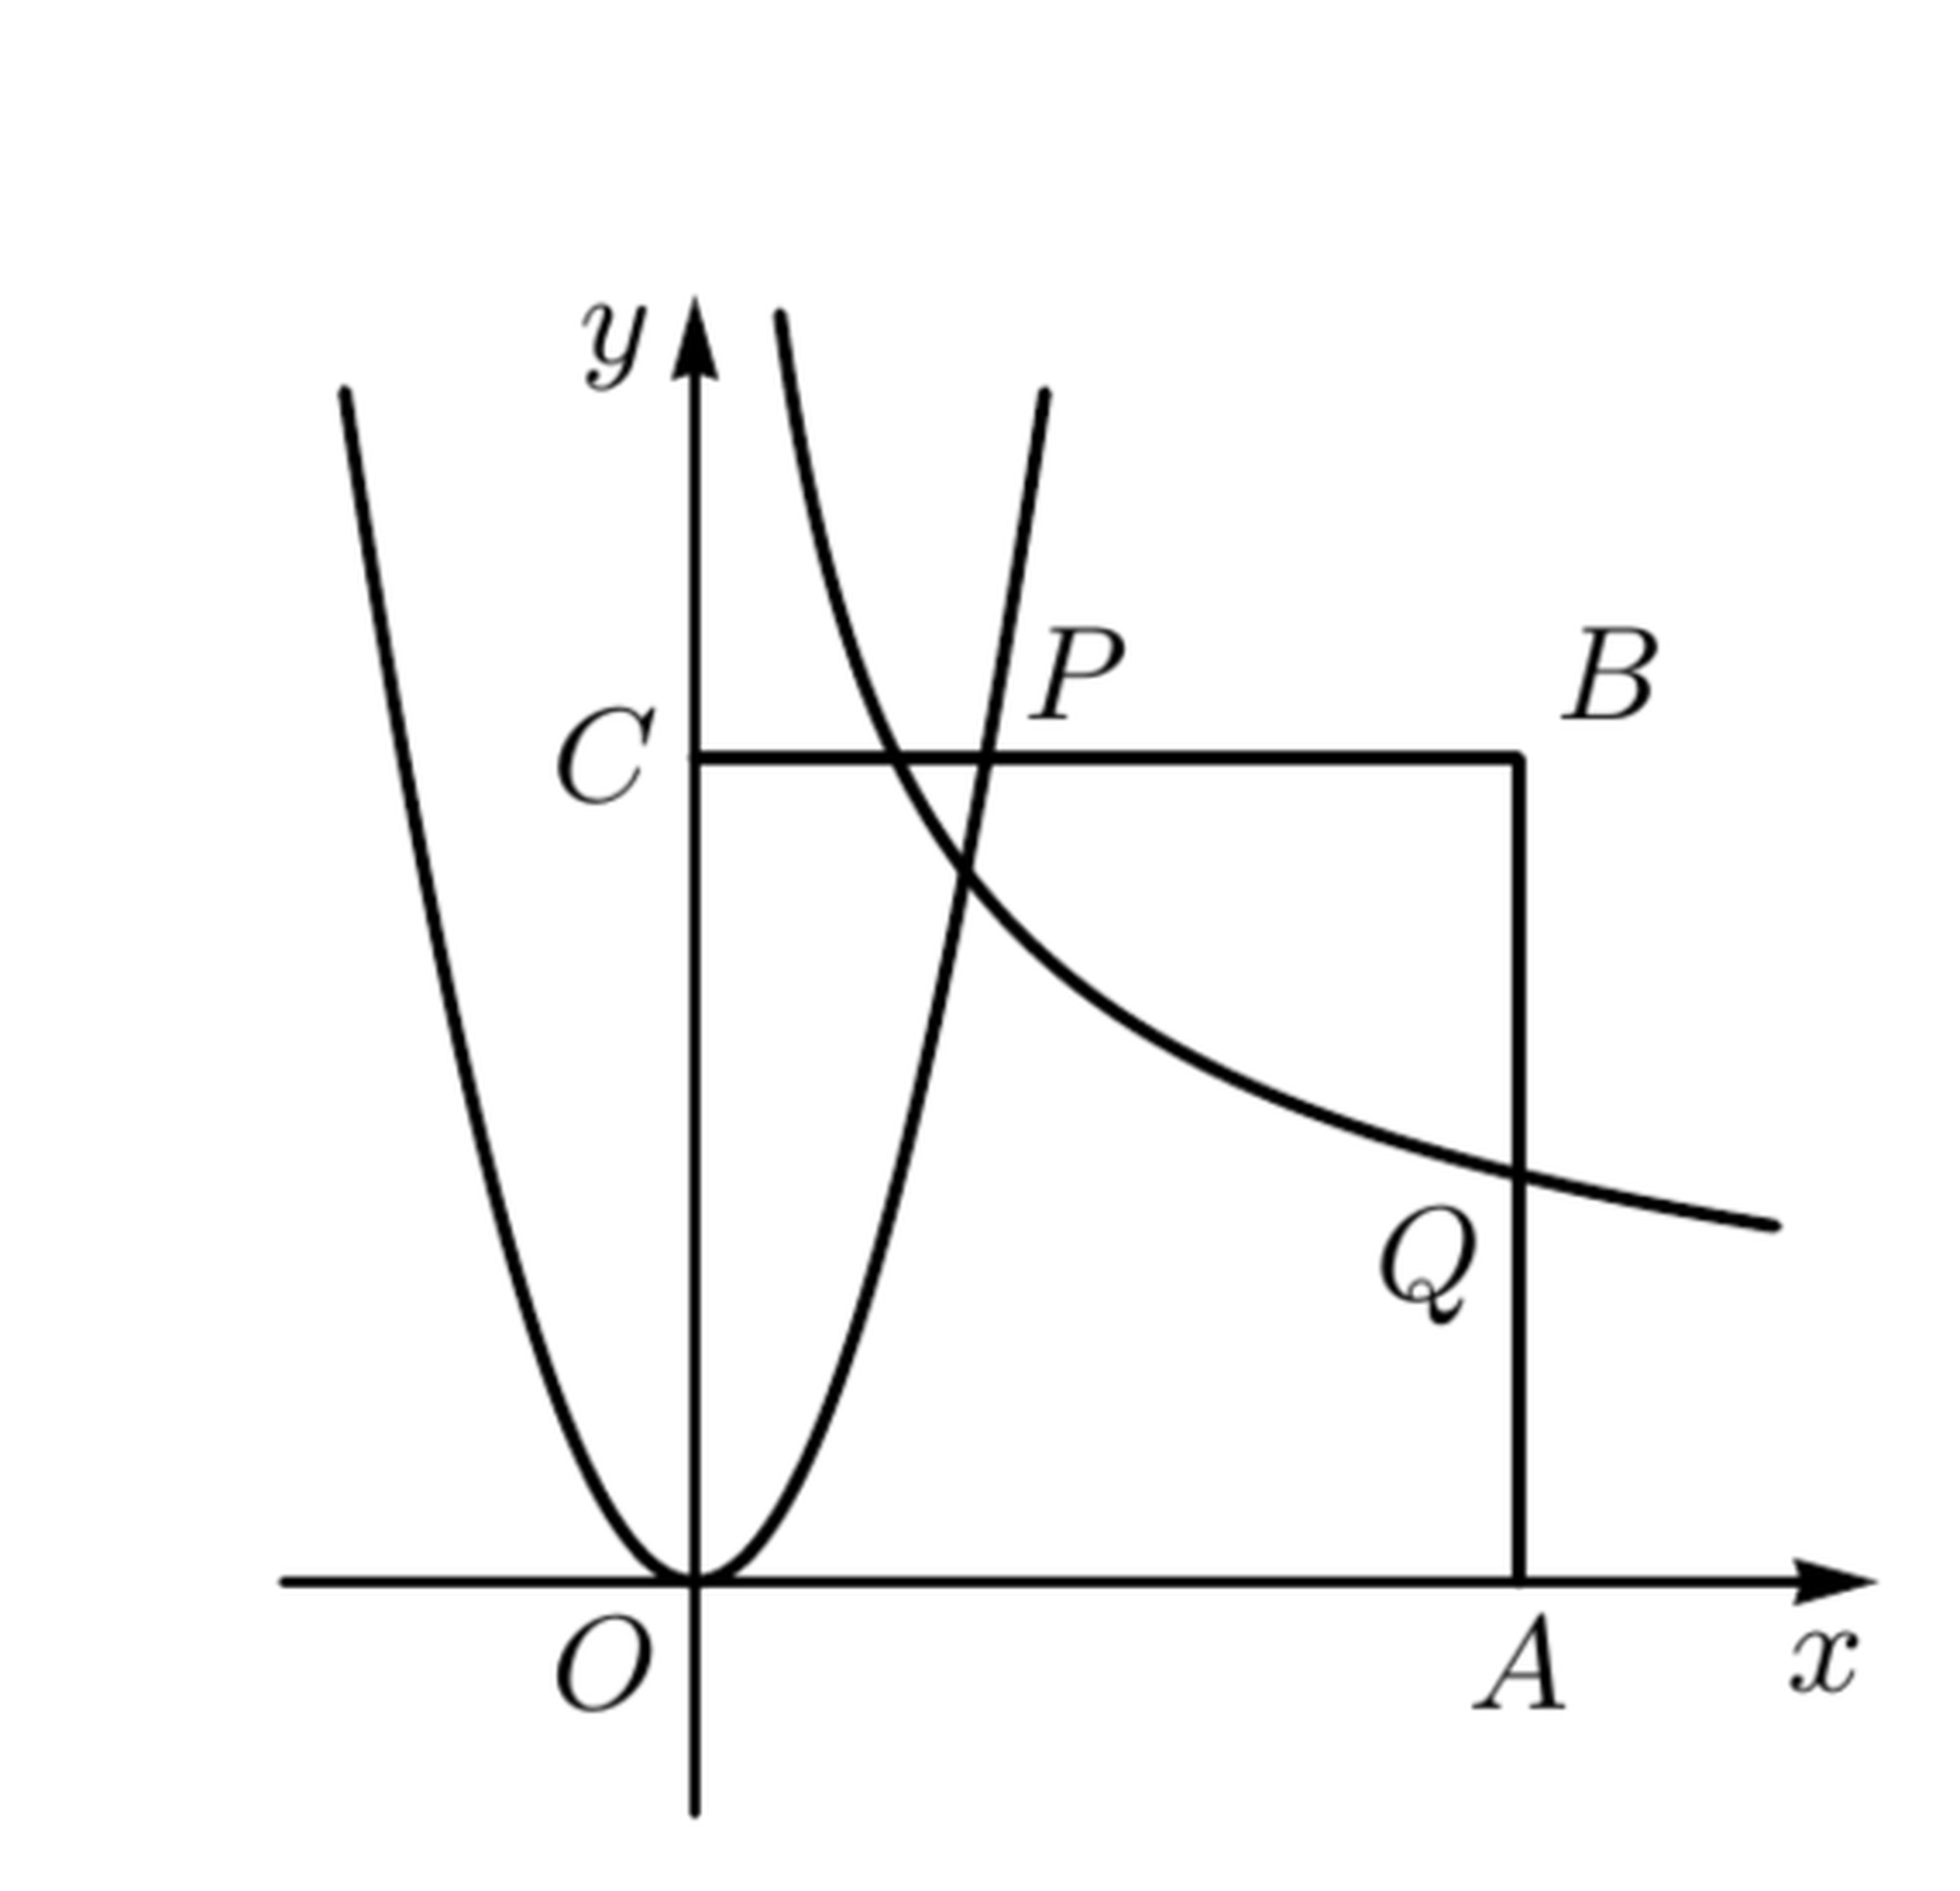
\includegraphics[width=0.40\textwidth]{figures/gao153_q11.png}
\end{center}

\ifanswer
\solbegin
\step{$\lvert AQ\rvert=\dfrac1{\sqrt a}$，$\lvert CP\rvert=\sqrt{\dfrac a5}$，}
\step{于是 $\lvert AQ\rvert+\lvert CP\rvert=\dfrac1{\sqrt a}+\sqrt{\dfrac a5}\geqslant2\sqrt{\dfrac1{\sqrt a}\cdot\sqrt{\dfrac a5}}=\dfrac2{\sqrt[4]{5}}$，}
\step{当且仅当 $\dfrac1{\sqrt a}=\sqrt{\dfrac a5}$，即 $a=\sqrt5$ 时取等号.}
\solend
\fi

% === Q12 === $B\subseteq A$ 带下划线照录、空集 \varnothing；解析 5 行
\item 若集合 $A=\{x\mid1\leqslant x\leqslant100,x\in\Z\}$，集合 $B\subseteq A$，且 $B\ne\varnothing$，记 $W(B)$ 为 $B$ 中元素的最大值与最小值之和，则对所有的 $B$，$W(B)$ 的平均值是\blankline[4.4em].

\ifanswer
\solbegin
\step{对每个非空子集 $B$，令 $B'=\{101-x\mid x\in B\}$，}
\step{则 $W(B')=(101-\min B)+(101-\max B)=202-W(B)$.}
\step{对 $B'$ 再作同样变换即得到 $B$，因此 $B$ 遍历所有非空子集时，}
\step{$B'$ 也恰好遍历所有非空子集.}
\step{设所求平均值为 $m$，则 $m=202-m$，解得 $m=101$.}
\solend
\fi

\end{enumerate}

\bigsec{二、选择题}

\begin{enumerate}
\setcounter{enumi}{12}

% === Q13 === "图像"（像，有亻）照录；解析 2 行，故选 A
\item 设 $a$、$b$ 为常数，若 $0<a<1$，$b>1$，则函数 $y=a^x-b$ 的图像必定不经过\mbox{（\quad）}

\keepwithprev
A. 第一象限\qquad\qquad B. 第二象限\qquad\qquad C. 第三象限\qquad\qquad D. 第四象限

\ifanswer
\solbegin
\step{当 $x>0$ 时，$a^x<1<b$，所以 $y=a^x-b<0$，图像必定不经过第一象限，}
\step{故选 $A$.}
\solend
\fi

% === Q14 === $m\in\Z$、中文弯引号、"图像"照录；解析 3 行，故选 A
\item 已知 $m\in\Z$，则“$m=0$”是“幂函数 $y=x^{m^2-2m-1}$ 的图像与 $x$ 轴及 $y$ 轴均无交点，且关于原点成中心对称”的\mbox{（\quad）}

\keepwithprev
A. 充分不必要条件\qquad\qquad B. 必要不充分条件

C. 充要条件\qquad\qquad D. 既不充分也不必要条件

\ifanswer
\solbegin
\step{图像满足所述条件 $\Leftrightarrow m^2-2m-1$ 为负奇数 $\Leftrightarrow m=0$ 或 $m=2$.}
\step{$m=0$ 能推出所述条件，但所述条件不能推出 $m=0$，因此是充分不必要条件，}
\step{故选 $A$.}
\solend
\fi

% === Q15 === 四选项一行；解析 5 行（跨 03→04 页），故选 D
\item 设 $a>b>1$，$x>1$，则下列不等式正确的是\mbox{（\quad）}

\keepwithprev
A. $a^x<b^x$\qquad B. $x^a<x^b$\qquad C. $\log_a x>\log_b x$\qquad D. $\log_x a>\log_x b$

\ifanswer
\solbegin
\step{$x>1$，幂函数与指数函数的单调性给出 $a^x>b^x$，$x^a>x^b$，A、B 错误.}
\step{$\log_a x=\dfrac{\lg x}{\lg a}<\dfrac{\lg x}{\lg b}=\log_b x$，C 错误.}
\step{对数函数 $y=\log_x t$ 的底数 $x>1$，在 $(0,+\infty)$ 上严格递增，}
\step{所以 $\log_x a>\log_x b$，D 正确.}
\step{故选 $D$.}
\solend
\fi

% === Q16 === $a\in\N$；解析 3 行，故选 C
\item 设 $a\in\N$，则满足不等式 $x^2-a^2x-a^2-1<0$ 的整数 $x$ 的个数不可能是\mbox{（\quad）}

\keepwithprev
A. 1\qquad\qquad B. 50\qquad\qquad C. 100\qquad\qquad D. 2026

\ifanswer
\solbegin
\step{$(x+1)(x-a^2-1)<0\Leftrightarrow-1<x<a^2+1$. 整数解为 $0,1,\cdots,a^2$，共 $a^2+1$ 个.}
\step{$1=0^2+1$，$50=7^2+1$，$2026=45^2+1$，而 $100-1=99$ 不是完全平方数，}
\step{故选 $C$.}
\solend
\fi

\end{enumerate}

\bigsec{三、解答题}

\begin{enumerate}
\setcounter{enumi}{16}

% === Q17 === 补集上划线 \overline{A}、\subseteq 照录；解析 5 行
\item 已知全集 $U=\R$，集合 $A=\{x\mid x^2-x-2\geqslant0\}$，$B=\{x\mid x>-1\}$，$C=\{x\mid a-5<x<a\}$.

(1) 求 $A\cap B$、$A\cup B$；

(2) 若 $\overline{A}\cup C=C$，求实数 $a$ 的取值范围.

\ifanswer
\solbegin
\step{(1) $x^2-x-2=(x+1)(x-2)\geqslant0\Leftrightarrow x\leqslant-1$ 或 $x\geqslant2$，}
\step{所以 $A=(-\infty,-1]\cup[2,+\infty)$，$B=(-1,+\infty)$，}
\step{因此 $A\cap B=[2,+\infty)$，$A\cup B=\R$.}
\step{(2) $\overline{A}=(-1,2)$，于是 $\overline{A}\cup C=C\Leftrightarrow\overline{A}\subseteq C\Leftrightarrow(-1,2)\subseteq(a-5,a)$，}
\step{两区间均为开区间，端点可重合，故 $\begin{cases}a-5\leqslant-1\\a\geqslant2\end{cases}\Leftrightarrow2\leqslant a\leqslant4$.}
\solend
\fi

% === Q18 === 解析 4 行
\item 已知 $a$、$b$、$c$ 都是正数，

(1) 若 $a+b=1$，求证：$\dfrac1a+\dfrac1b\geqslant4$，并指出等号成立的条件；

(2) 若 $a+b+c=1$，求证：三个数 $\dfrac1a$、$\dfrac1b$、$\dfrac1c$ 中至少有一个不小于 3.

\ifanswer
\solbegin
\step{(1) 由 $(a-b)^2\geqslant0$，得 $4ab\leqslant(a+b)^2=1$，所以 $\dfrac1a+\dfrac1b=\dfrac{a+b}{ab}=\dfrac1{ab}\geqslant4$，}
\step{等号成立当且仅当 $a=b$，结合 $a+b=1$，得 $a=b=\dfrac12$.}
\step{(2) 假设三个数 $\dfrac1a$、$\dfrac1b$、$\dfrac1c$ 都小于 3，则 $a>\dfrac13,b>\dfrac13,c>\dfrac13\Rightarrow a+b+c>1$，}
\step{与 $a+b+c=1$ 矛盾，因此三个数中至少有一个不小于 3.}
\solend
\fi

% === Q19 === 题目配图（三版都出）；\needvspace 守卫放 \item 之前；解析 19 行
\needvspace{8cm}
\item 某新建居民小区有一直角三角形绿地，两直角边长分别为 30m 和 40m，打算在其中划出一片区域改造成活动场地，如图所示.

(1) 若划出的区域为正方形，且有两边落在绿地边界上，求此正方形边长；

(2) 若划出的区域为圆形，求圆形区域面积的最大值；

(3) 若划出的区域为矩形（其中至少有一边在边界上），求此矩形面积的最大值.

\begin{center}
% 直角三角形 ABC 绿地示意图取 05 页右上，去粉色水印、去色、4× LANCZOS 放大；三版都出
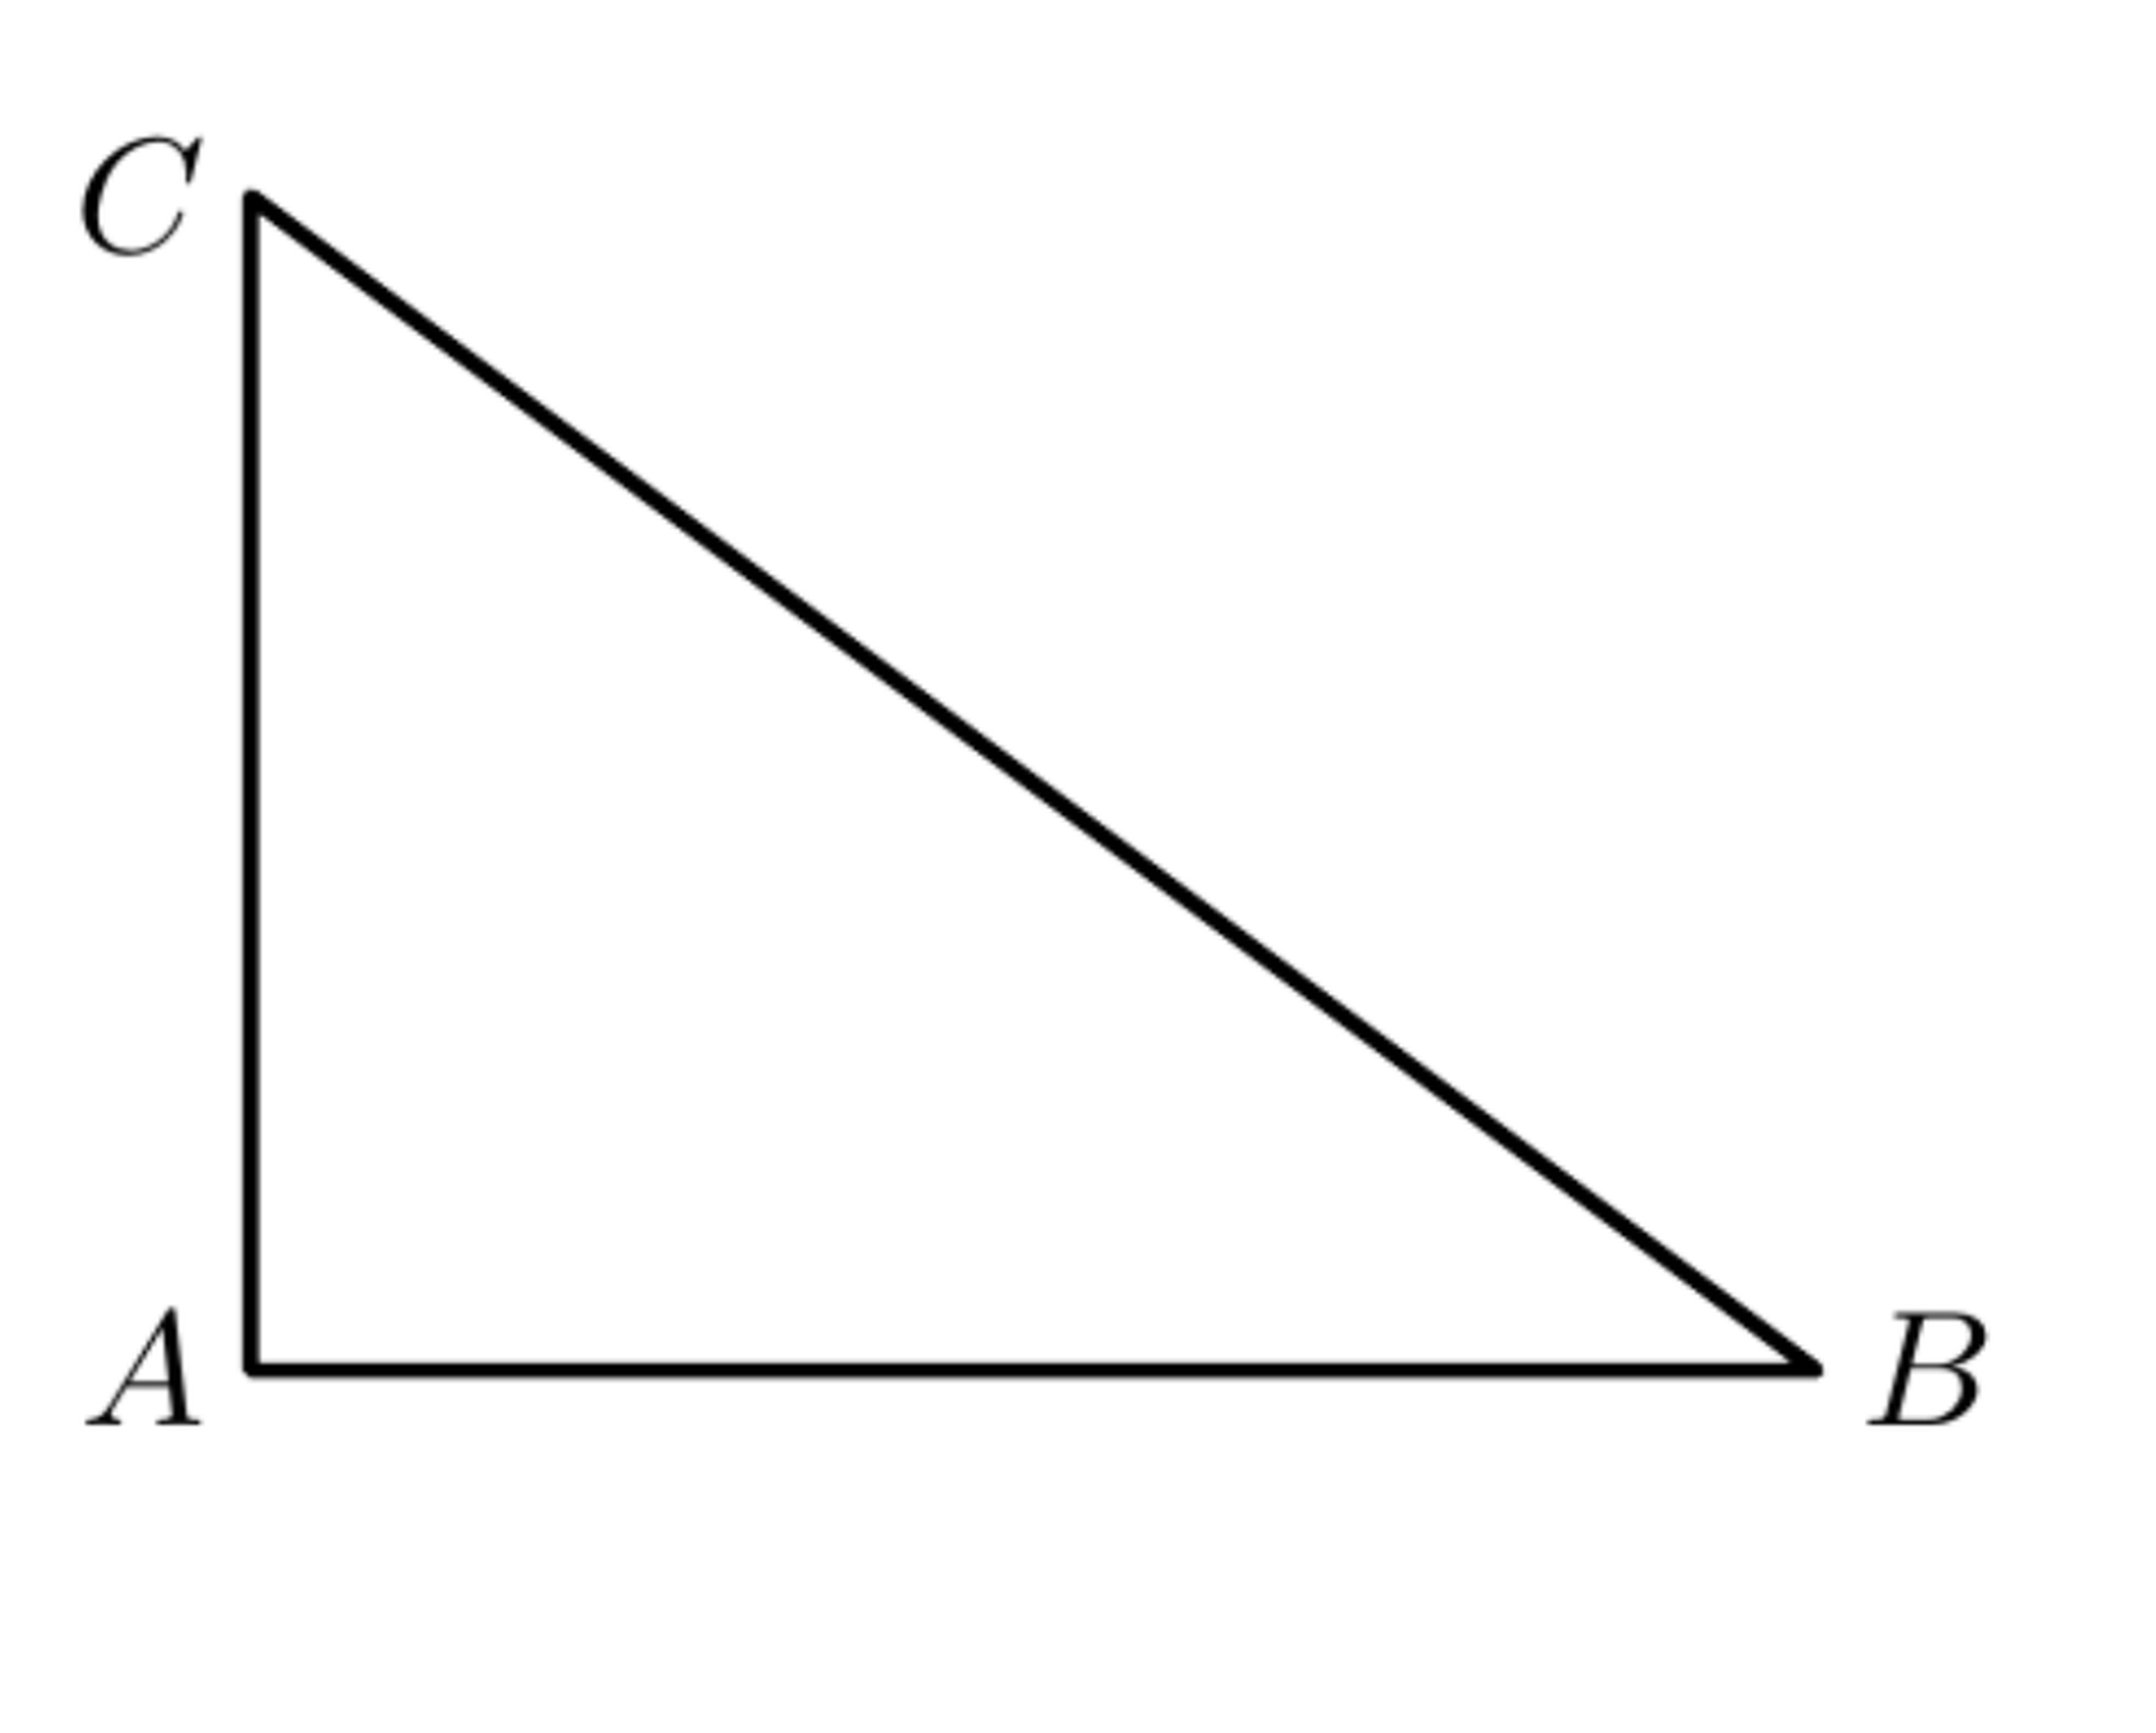
\includegraphics[width=0.34\textwidth]{figures/gao153_q19.png}
\end{center}

\ifanswer
\solbegin
\step{(1) 取 $A(0,0)$、$B(40,0)$、$C(0,30)$，则斜边 $BC$ 所在直线为 $3x+4y=120$.}
\step{正方形落在边界上的两边必分别在两条直角边上.}
\step{设其边长为 $a$m，则对角顶点为 $(a,a)$.}
\step{按题意划出的正方形应尽量大，即对角顶点落在斜边 $BC$ 上，}
\step{因此 $3a+4a=120\Rightarrow a=\dfrac{120}{7}$；}
\step{(2) 斜边长 $BC=\sqrt{30^2+40^2}=50$m，三角形面积为 $600\text{m}^2$.}
\step{设圆的半径为 $r$，圆心到 $AB$、$AC$、$BC$ 的距离分别为 $d_1,d_2,d_3$，}
\step{则三者均不小于 $r$. 连接圆心与三个顶点，}
\step{得 $600=\dfrac12(40d_1+30d_2+50d_3)\geqslant\dfrac12(40+30+50)r=60r$，所以 $r\leqslant10$.}
\step{取三角形的内切圆时等号成立，圆形区域面积的最大值为 $100\pi\text{m}^2$.}
\step{(3) 任取矩形落在绿地边界上的一边，以其所在直线为横轴.}
\step{设相应三角形底边长为 $L$、高为 $H$，则 $LH=1200$.}
\step{取三角形顶点坐标为 $(0,0)$、$(L,0)$、$(p,H)$.}
\step{在高度 $t$ 处，两腰上的点的横坐标分别为 $\dfrac{pt}{H}$、$L+\dfrac{(p-L)t}{H}$，}
\step{因此，高为 $t$ 的矩形，其底边长不超过 $L\left(1-\dfrac tH\right)$，}
\step{面积满足 $S\leqslant Lt\left(1-\dfrac tH\right)=\dfrac LH\left[\dfrac{H^2}{4}-\left(t-\dfrac H2\right)^2\right]\leqslant\dfrac{LH}{4}=300$，}
\step{在原坐标系中，取矩形顶点为 $(0,0)$、$(20,0)$、$(20,15)$、$(0,15)$，}
\step{其中 $3\times20+4\times15=120$，矩形完全位于绿地内，面积为 $300\text{m}^2$，}
\step{达到最大值.}
\solend
\fi

% === Q20 === $g(x)$ 定义照录；解析 14 行
\item 已知 $a>0$ 且 $a\ne1$，设 $f(x)=\log_a(x^2-a^2)$，$g(x)=2\log_a(x-ak)$.

(1) 求函数 $y=f(x)$ 的定义域；

(2) 若 $k=2$，求不等式 $f(x)>g(x)$ 的解集；

(3) 若“存在实数 $x$，使得 $f(x)=g(x)$”为真命题，求实数 $k$ 的取值范围.

\ifanswer
\solbegin
\step{(1) $x^2-a^2>0\Leftrightarrow x<-a$ 或 $x>a$，定义域为 $(-\infty,-a)\cup(a,+\infty)$.}
\step{(2) 两函数均有意义时，$x>2a$，且 $g(x)=\log_a(x-2a)^2$.}
\step{当 $a>1$ 时，$f(x)>g(x)\Leftrightarrow x^2-a^2>(x-2a)^2\Leftrightarrow x>\dfrac{5a}{4}$，}
\step{结合 $x>2a$，解集为 $(2a,+\infty)$.}
\step{当 $0<a<1$ 时，$f(x)>g(x)\Leftrightarrow x^2-a^2<(x-2a)^2\Leftrightarrow x<\dfrac{5a}{4}$，}
\step{与 $x>2a$ 矛盾，解集为 $\varnothing$.}
\step{(3) 在 $x^2-a^2>0$ 且 $x-ak>0$ 的条件下，}
\step{$f(x)=g(x)\Leftrightarrow x^2-a^2=(x-ak)^2\Leftrightarrow2akx=a^2(1+k^2)$，}
\step{当 $k=0$ 时，上式不成立；}
\step{当 $k\ne0$ 时，$x=\dfrac{a(1+k^2)}{2k}$，}
\step{于是 $x-ak=\dfrac{a(1-k^2)}{2k}>0\Leftrightarrow k<-1$ 或 $0<k<1$，}
\step{对上述 $k$，所取的 $x$ 同时满足 $x^2-a^2=(x-ak)^2>0$，}
\step{两函数均有意义且函数值相等.}
\step{因此，$k$ 的取值范围为 $(-\infty,-1)\cup(0,1)$.}
\solend
\fi

% === Q21 === 中文弯引号、复杂式照录；解析 23 行（跨 08→09 页）
\item 若实数 $x$、$y$、$m$ 满足 $\lvert x-m\rvert<\lvert y-m\rvert$，则称 $x$ 比 $y$ 接近 $m$.

(1) 若 $2x$ 比 $x-2$ 更接近 1，求实数 $x$ 的取值范围；

(2) 若 $x$ 比 $y$ 接近 $m$，证明：“$x>y$” 的充要条件是 “$x+y<2m$”；

(3) 已知 $x>0$，$y>0$ 且 $x\ne y$. 设 $p=\dfrac{x^2+y^2}{xy}$，若对于任意的 $x$、$y$，命题 “$p$ 比 $p^2-3p+4$ 接近 $m$” 恒成立，求实数 $m$ 的取值范围.

\ifanswer
\solbegin
\step{(1) $\lvert2x-1\rvert<\lvert x-3\rvert\Leftrightarrow(2x-1)^2<(x-3)^2\Leftrightarrow(x+2)(3x-4)<0$，}
\step{解得 $-2<x<\dfrac43$，实数 $x$ 的取值范围为 $\left(-2,\dfrac43\right)$.}
\step{(2) 因为 $x$ 比 $y$ 接近 $m$，所以 $\lvert x-m\rvert<\lvert y-m\rvert$，则 $\lvert x-m\rvert^2<\lvert y-m\rvert^2$，}
\step{即 $(x-m)^2<(y-m)^2$，即 $(x-m)^2-(y-m)^2<0$，}
\step{即得 $(x-y)(x+y-2m)<0$，}
\step{则由 $x+y<2m$，得 $x+y-2m<0$，}
\step{故 $x-y>0$，即 $x>y$，充分性成立；}
\step{当 $x>y$ 时，$x-y>0$，结合 $(x-y)(x+y-2m)<0$，得 $x+y-2m<0$，}
\step{即 $x+y<2m$，必要性成立；}
\step{故“$x>y$” 的充要条件是 “$x+y<2m$”；}
\step{(3) $x>0$，$y>0$ 且 $x\ne y$. 则 $p=\dfrac{x^2+y^2}{xy}=\dfrac xy+\dfrac yx>2\sqrt{\dfrac xy\cdot\dfrac yx}=2$，}
\step{由于对于任意的 $x$、$y$，命题 “$p$ 比 $p^2-3p+4$ 接近 $m$” 恒成立，}
\step{故 $\lvert p-m\rvert<\lvert(p^2-3p+4)-m\rvert$ 对 $\forall p>2$ 恒成立，}
\step{即得 $(p-m)^2<(p^2-3p+4-m)^2$，}
\step{即 $(p^2-3p+4-m)^2-(p-m)^2>0$，}
\step{得 $(p^2-4p+4)(p^2-2p+4-2m)>0$，}
\step{即 $(p-2)^2(p^2-2p+4-2m)>0$，由于 $p>2$，故 $(p-2)^2>0$，}
\step{故 $p^2-2p+4-2m>0$ 对 $\forall p>2$ 恒成立，}
\step{即 $2m<p^2-2p+4$ 对 $\forall p>2$ 恒成立，}
\step{由于 $p^2-2p+4=(p-1)^2+3$，此时 $p^2-2p+4$ 在 $(2,+\infty)$ 上严格增，}
\step{故 $(p-1)^2+3>(2-1)^2+3=4$，故 $2m\leqslant4$，解得 $m\leqslant2$，}
\step{即实数 $m$ 的取值范围是 $(-\infty,2]$.}
\solend
\fi

\end{enumerate}

\end{document}
"
%
% ① 原始材料：微信公众号"魔都数学加油站"文章，连载"27学年高一153"，原文标题
% "27学年高一153——2026-2027年上海市闵行中学文绮中学高一上期中"；
% 原文链接：https://mp.weixin.qq.com/s/rEtS-92cDR6JKgY2b5DRfg 。
% 正文为 9 张 PNG 页（01/02/06/07/08/09 为 2560×3620，03/04/05 为 4762×6735，
% 同一篇各页分辨率混排，逐页按各自分辨率裁图核对，别按预览比例换算裁框）。
% 体例：讲评版——填空 3—12（10 题）、选择 13—16（4 题）、解答 17—21（5 题），
% 共 19 题，自第 3 题起编；**全 19 题均印【解析】**（逐题核实，见 ② ②）。
% 题目、答案、解析均据原图转录；卷面粉红色水印"魔都数学加油站"及公众号页脚未录入。
% 全卷插图清单（逐页通读 9 页确认）：2 幅，均为题目配图、三版都出——
%   · Q11 正方形 OABC 曲线图（02 页右下：$y=5x^2$ 与 $y=x^{-\frac12}$ 两条曲线、
%     坐标轴、O/A/B/C/P/Q、正方形），裁 figures/gao153_q11.png；
%   · Q19 直角三角形 ABC 绿地示意图（05 页右上，直角在 A），
%     裁 figures/gao153_q19.png；
%   两图均去粉色水印、去色、4× LANCZOS 放大；Q11 图左上角题干残字"函"已裁白。
%   其余各页逐页确认无其它题目配图、无解析内配图、无表格；09 页下半仅水印、无正文。
%
% 卷首标题：原卷印作"2026-2027 年闵行中学文绮中学高一上期中"，年份区间按全稿惯例排 en dash；
% 原卷卷面未印副标题，本稿按同期中卷知识模块口径补出"集合与常用逻辑用语、不等式、函数"。
%
% ② 与原卷的排版差异：
%   ① 原文从第 3 题起，本稿保留原题号；共 19 题三节，解答题 5 题到 21；
%   ② 全 19 题均印【解析】、用 \solbegin…\solend，无只印【答案】或答案印括号内的题；
%      四道选择题答案在解析末句"故选 A／A／D／C"（Q13—Q16，逐个放大复核）、
%      括号 \mbox{（\quad）} 留空、不另提 \ans{}；答案版【答案】/【解析】标记数
%      = 19 = 全卷题数；
%   ③ 原卷卷面未印副标题，本稿按知识模块口径补出；
%   ④ 原卷填空横线按全稿惯例排 \blankline[4.4em]；选择题括号排 \mbox{（\quad）}、
%      四道选择题的选项段前按惯例各加 \keepwithprev；解答题不留作答区、不加
%      \anspace（原卷为讲评版，109—113 起全稿不用 \anspace）；
%   ⑤ 数集：Q3"$x\in R$"、Q5"解集为 R"、Q10"$x\in N$"、Q12"$x\in Z$"与
%      "$m\in Z$"、Q14"$m\in Z$"、Q16"$a\in N$"、Q17"全集 $U=R$"、
%      Q19 无、Q21 无——原卷印斜体或正体粗体 R/N/Z，按全稿惯例归一
%      \R／\N／\Z；绝对值排 \lvert…\rvert（Q5、Q11、Q21），集合描述竖线排 \mid
%      （Q3、Q10、Q17、Q20），不等号按全稿惯例排 \leqslant／\geqslant；
%      补集照原卷上划线排 \overline{A}（Q17 题干 (2)＋解析 (2)）；
%      空集 \varnothing（Q12 题干、Q20 解析 (2)）；子集 3 处均印带下划线 ⊆、
%      照录 \subseteq（Q10 $A\subseteq U$、Q12 $B\subseteq A$、Q17 $(-1,2)\subseteq(a-5,a)$），
%      本卷无单线 \subset 用例；
%   ⑥ 判别式：逐页通读 9 页，本卷无一元二次判别式 Δ/△ 算式，故无 Δ/△ 混用可照录；
%      Q11 图里有几何正方形 OABC（非三角形符号），无 △ABC 用例；
%   ⑦ 中文弯引号照录：Q14"$m=0$"与"幂函数…关于原点成中心对称"、
%      Q20"存在实数 $x$，使得 $f(x)=g(x)$"、Q21"$x>y$"与"$x+y<2m$"、
%      "$p$ 比 $p^2-3p+4$ 接近 $m$"（引号外留空格按原卷）；
%      注释里一律 ASCII 引号；数学式内 CJK 用 \text{}；
%   ⑧ "图像／图象"逐处放大核：全卷 3 处均印"图像"（像，有亻）——
%      Q13 题干与解析、Q14 题干与解析；Q19 题干写"如图所示"（非"图像"），
%      逐处照录未统一；子题标号 (1)(2)(3) 半角括号照录；圈数字本卷无用例；
%   ⑨ 半角逗号在数学组之间是全稿惯例、非笔误，逐处照录（Q3 $x\in R$、
%      Q10 $a_1,a_2$、Q19 $A(0,0)$、$d_1,d_2,d_3$、Q21 $a>\frac13,b>\frac13$ 等）；
%      行末西文句点 ASCII `.`；行中全角逗号／顿号照录（Q19"30m 和 40m"、
%      Q21"实数 $x$、$y$、$m$"）；
%   ⑩ 复杂式照录别简化：Q3 $y=x^{-2}$、Q11 $y=x^{-\frac12}$ 与
%      $\frac{2}{\sqrt[4]{5}}$、Q8 $\frac{2b}{a+1-b}$、Q9 cases 块、
%      Q10 $525=5\times105$、Q16 $a^2+1$、Q19 $S\leqslant Lt(1-\frac tH)$
%      与 $L+\frac{(p-L)t}{H}$、Q20 $2akx=a^2(1+k^2)$ 与 $\frac{a(1+k^2)}{2k}$、
%      Q21 $(p^2-4p+4)(p^2-2p+4-2m)>0$；
%      \left…\right 不得拆到不同 $…$ 组（Q17 $\left\{x\mid\cdots\right\}$、
%      Q19 $\left[\frac{H^2}{4}-\left(t-\frac H2\right)^2\right]$、
%      Q21 $\left(-2,\frac43\right)$ 等）；cases 块一律 \begin{cases}…\end{cases}；
%   ⑪ 一条 \step = 原卷解析的一个印刷行，cases 块整体算一个印刷行；别并折行、
%      别拆行。Q10 六行、Q19 十九行、Q20 十四行、Q21 二十二行均按印刷行逐条断，
%      不丢行；
%   ⑫ 配图：Q11／Q19 题目配图（三版都出）放 \item 内题干之后 \begin{center}，
%      各用 \needvspace{8cm} 守卫把整块推走，**守卫放在 \item 之前**
%      （见 高一145 Q14/Q20 成例与切页审计 B 类坑）；
%   ⑬ 原卷解析内无红色"法一／法二"之类小标题，故本卷无 \stepm；红色水印
%      "魔都数学加油站"不录入；
%   ⑭ 跨页续印按题合并：见 ⑥；
%
% ③ 行数复核：一条 \step = 原卷解析的一个印刷行，cases 块作一个印刷行计。
%   逐题数（主会话逐页核对定稿）：Q3：1；Q4：2；Q5：2；Q6：2；Q7：1；
%   Q8：1；Q9：2；Q10：6；Q11：3；Q12：5；Q13：2；Q14：3；Q15：5；
%   Q16：3；Q17：5；Q18：4；Q19：19；Q20：14；Q21：22。
%   合计 102 条 \step（本卷无 \stepm），与原卷逐题印刷行相等。全卷 19 题
%   均设 \solbegin…\solend，答案版【答案】/【解析】标记数 = 19 = 全卷题数。
%
% ④ 判别式／子集符号结论（逐处放大原图照录、不得统一，主会话像素级复核）：
%   判别式：逐页通读 9 页，本卷无一元二次判别式算式（Q7 用韦达定理、
%      Q16 用因式分解、Q20 用对数方程，均不写 Δ/△），故无 Δ/△ 混用可照录
%      （"高 \Delta／扁 \triangle"口径备查，参照 高一142／151／152 头注）；
%      本卷无几何三角形符号用例。
%   子集：Q10 题干"$A\subseteq U$"、Q12 题干"$B\subseteq A$"、Q17 解析 (2)
%      "$(-1,2)\subseteq(a-5,a)$"共 3 处，逐处放大确认均印带下划线 ⊆、
%      照录 \subseteq；本卷未见单线 ⊂（\subset）之对应处。
%      补集上划线 \overline{A}（Q17）、空集 \varnothing（Q12 题干、Q20 解析 (2)）；
%      数集 \R／\N／\Z 归一见 ② ⑤。
%
% ⑤ 存疑照录（放大原图确认，照录未改、正文对应处另有 % 注）：
%   1. Q3 集合 $B=\{(x,y)\mid y=x^{-2},x\in\R\}$ 原卷题干径写 $x\in\R$
%      （$x=0$ 处无意义），解析自行注明 $x\ne0$，照录未改。
%   2. Q10 解析"$U$ 中共有 $525=5\times105$ 个连续整数"与尾行
%      "取 $U$ 中除以 5 余 1 或 2 的全部元素及元素 5"逐字照录（放大 02 页
%      /tmp/gao153/z/zoom/q10_pick.png 确认是"元素 5"，非"元素 9"）。
%   3. Q11 第二个函数原卷印 $y=x^{-\frac12}$（负二分之一次幂，非 $x^2$），
%      放大 02 页 /tmp/gao153/z/zoom/q11_exp.png 确认，照录未改；
%      $|AQ|=\frac1{\sqrt a}$ 与之自洽。
%   4. Q19 (3) 解析"在高度 $t$ 处，两腰上的点的横坐标分别为 $\frac{pt}{H}$、
%      $L+\frac{(p-L)t}{H}$"，放大 06 页确认，照录未简化。
%   5. Q20 (2) 解析"$g(x)=\log_a(x-2a)^2$"（真数整体平方），
%      与 $g(x)=2\log_a(x-ak)$ 在 $k=2$ 时一致，照录未改。
%   6. Q21 (3) 解析"得 $(p^2-4p+4)(p^2-2p+4-2m)>0$"与
%      "故 $(p-1)^2+3>(2-1)^2+3=4$，故 $2m\leqslant4$"照录未改
%      （放大 09 页 /tmp/gao153/z/zoom/q21_factor.png 确认）。
%   7. "图像／图象"全卷 3 处均印"图像"（像，有亻）逐处照录；
%      本卷无判别式 Δ/△ 用例（见 ④）。
%   全卷除此 7 类外未发现其它笔误／自相矛盾处；19 题均印【解析】、
%   无只印【答案】或答案印括号内的题（见 ② ②）。
%
% ⑥ 跨页续印按题合并说明（逐页核实定稿）：Q3—Q5 题干＋解析在 01 页；
%   Q6—Q8 题干＋解析在 01 页下半（Q8 解析续 02 页顶）；Q9 题干＋解析、
%   Q10 题干＋解析首 2 行在 02 页上半，Q10 解析余 4 行在 02 页下半；
%   Q11 题干＋配图＋解析、Q12 题干＋解析 5 行在 02 页下半—03 页上半；
%   "二、选择题"标题在 03 页中部；Q13 题干＋选项＋解析在 03 页下半；
%   Q14 题干＋选项＋解析、Q15 题干＋选项＋解析首行在 03 页下半—04 页顶；
%   Q15 解析余 4 行、Q16 题干＋选项＋解析在 04 页上半；"三、解答题"
%   标题在 04 页下半；Q17 题干＋两问＋解析 5 行在 04 页下半—05 页顶；
%   Q18 题干＋两问＋解析 4 行、Q19 题干（含配图）＋三问在 05 页；
%   Q19 解析 (1)(2) 9 行在 05 页下半，解析 (3) 前 5 行在 06 页上半、
%   余 4 行在 06 页下半；Q20 题干＋三问在 06 页下半，解析 (1)(2)(3)
%   前 6 行在 07 页上半、(3) 余 8 行在 07 页下半；Q21 题干＋三问在
%   07 页末，解析 (1)(2) 10 行在 08 页上半—下半，解析 (3) 前 4 行在
%   08 页下半、余 9 行续 09 页上半，末行"即实数 $m$ 的取值范围是
%   $(-\infty,2]$"为全卷收尾（09 页下半仅水印、无正文）。
%   本稿按题连排，不丢行、不并折行；全卷末题为第 21 题，无附加题节。
%
\documentclass[a4paper,11pt]{article}
\usepackage{common}

\begin{document}

\examtitlest[3]{2026--2027 年闵行中学文绮中学高一上期中}{集合与常用逻辑用语、不等式、函数}

\bigsec{一、填空题}

\begin{enumerate}
\setcounter{enumi}{2}

% === Q3 === 集合描述竖线 \mid；$y=x^{-2}$ 照录；解析 1 行
\item 已知 $A=\{(x,y)\mid y=x^3,x\in\R\}$，$B=\{(x,y)\mid y=x^{-2},x\in\R\}$，则 $A\cap B=$\blankline[4.4em].

\ifanswer
\solbegin
\step{$x^3=x^{-2}\ (x\ne0)\Leftrightarrow x^5=1\Leftrightarrow x=1$，此时 $y=1$，所以 $A\cap B=\{(1,1)\}$.}
\solend
\fi

% === Q4 === 解析 2 行
\item 若关于 $x$ 的不等式 $\dfrac{x-a}{x+1}>0$ 的解集为 $(-\infty,-1)\cup(4,+\infty)$，则实数 $a=$\blankline[4.4em].

\ifanswer
\solbegin
\step{关于 $x$ 的不等式 $\dfrac{x-a}{x+1}>0$ 即 $(x+1)(x-a)>0$.}
\step{再由它的解集为 $(-\infty,-1)\cup(4,+\infty)$，得 $-1$ 和 4 是 $(x+1)(x-a)=0$ 的两个实数根，故 $a=4$.}
\solend
\fi

% === Q5 === 绝对值 \lvert…\rvert；解析 2 行
\item 若关于 $x$ 的不等式 $\lvert x+1\rvert+\lvert x-2\rvert>m$ 的解集为 $\R$，则实数 $m$ 的取值范围是\blankline[4.4em].

\ifanswer
\solbegin
\step{$\lvert x+1\rvert+\lvert x-2\rvert\geqslant\lvert(x+1)-(x-2)\rvert=3$，当且仅当 $-1\leqslant x\leqslant2$ 时取等号，}
\step{因此 $m<3$.}
\solend
\fi

% === Q6 === 解析 2 行
\item 已知指数函数 $y=a^x$（$a>1$）在区间 $[-1,1]$ 上的最大值比最小值大 $\dfrac32$，则实数 $a=$\blankline[4.4em].

\ifanswer
\solbegin
\step{$a>1$，指数函数在 $[-1,1]$ 上严格增，故 $a-\dfrac1a=\dfrac32\Leftrightarrow(a-2)(2a+1)=0$.}
\step{结合 $a>1$，得 $a=2$.}
\solend
\fi

% === Q7 === 韦达定理；解析 1 行
\item 已知关于 $x$ 的一元二次方程 $x^2+px+2p=0$ 的两个实数根分别为 $x_1$、$x_2$，且 $(x_1+1)(x_2+1)=0$，则 $p=$\blankline[4.4em].

\ifanswer
\solbegin
\step{$0=(x_1+1)(x_2+1)=x_1x_2+x_1+x_2+1=2p-p+1=p+1\Rightarrow p=-1$.}
\solend
\fi

% === Q8 === 换底公式；解析 1 行
\item 已知 $10^a=3$，$\lg5=b$，则 $\log_6 25=$\blankline[4.4em]（用关于 $a,b$ 的关系式表示）.

\ifanswer
\solbegin
\step{$\lg3=a$，$\lg2=1-b$，所以 $\log_6 25=\dfrac{\lg25}{\lg6}=\dfrac{2b}{a+1-b}$.}
\solend
\fi

% === Q9 === cases 块整体算一个印刷行；解析 2 行
\item 已知 $A=[2,5]$，若对任意 $x\in A$，总有 $\dfrac{k}{x}\in A$，则正数 $k=$\blankline[4.4em].

\ifanswer
\solbegin
\step{$k>0$，当 $x\in[2,5]$ 时，$\dfrac{k}{x}$ 的取值范围为 $\left[\dfrac k5,\dfrac k2\right]$，}
\step{因此 $\begin{cases}\dfrac k5\geqslant2\\\dfrac k2\leqslant5\end{cases}\Leftrightarrow10\leqslant k\leqslant10\Leftrightarrow k=10$.}
\solend
\fi

% === Q10 === $A\subseteq U$ 带下划线照录；解析 6 行
\item 已知集合 $U=\{x\mid4\leqslant x\leqslant528,x\in\N\}$，$A=\{a_1,a_2,a_3,\cdots,a_n\}$，且 $A\subseteq U$. 如果集合 $A$ 中的任意两个不同元素之和都不能被 5 整除，则正整数 $n$ 的最大值为\blankline[4.4em].

\ifanswer
\solbegin
\step{$U$ 中共有 $525=5\times105$ 个连续整数，按除以 5 的余数分成五类，}
\step{每类均有 105 个元素.}
\step{余数为 1,4 的两类不能同时选取，余数为 2,3 的两类也不能同时选取，}
\step{余数为 0 的一类最多选 1 个，因此 $n\leqslant105+105+1=211$.}
\step{取 $U$ 中除以 5 余 1 或 2 的全部元素及元素 5，}% 放大 02 页确认是「元素 5」（非 9），照录未改（见 ⑤ 2）
\step{任意两个不同元素之和均不能被 5 整除，此时 $n=211$，最大值为 211.}
\solend
\fi

% === Q11 === 题目配图（三版都出）；\needvspace 守卫放 \item 之前；$y=x^{-\frac12}$ 照录；解析 3 行
\needvspace{8cm}
\item 如图，已知正方形 $OABC$，其中 $OA=a$（$a>1$），函数 $y=5x^2$ 交 $BC$ 于点 $P$，函数 $y=x^{-\frac12}$ 交 $AB$ 于点 $Q$，当 $\lvert AQ\rvert+\lvert CP\rvert$ 最小时，$a$ 的值为\blankline[4.4em].

\begin{center}
% 正方形 OABC 与两条曲线图取 02 页右下，去粉色水印、去色、4× LANCZOS 放大；三版都出
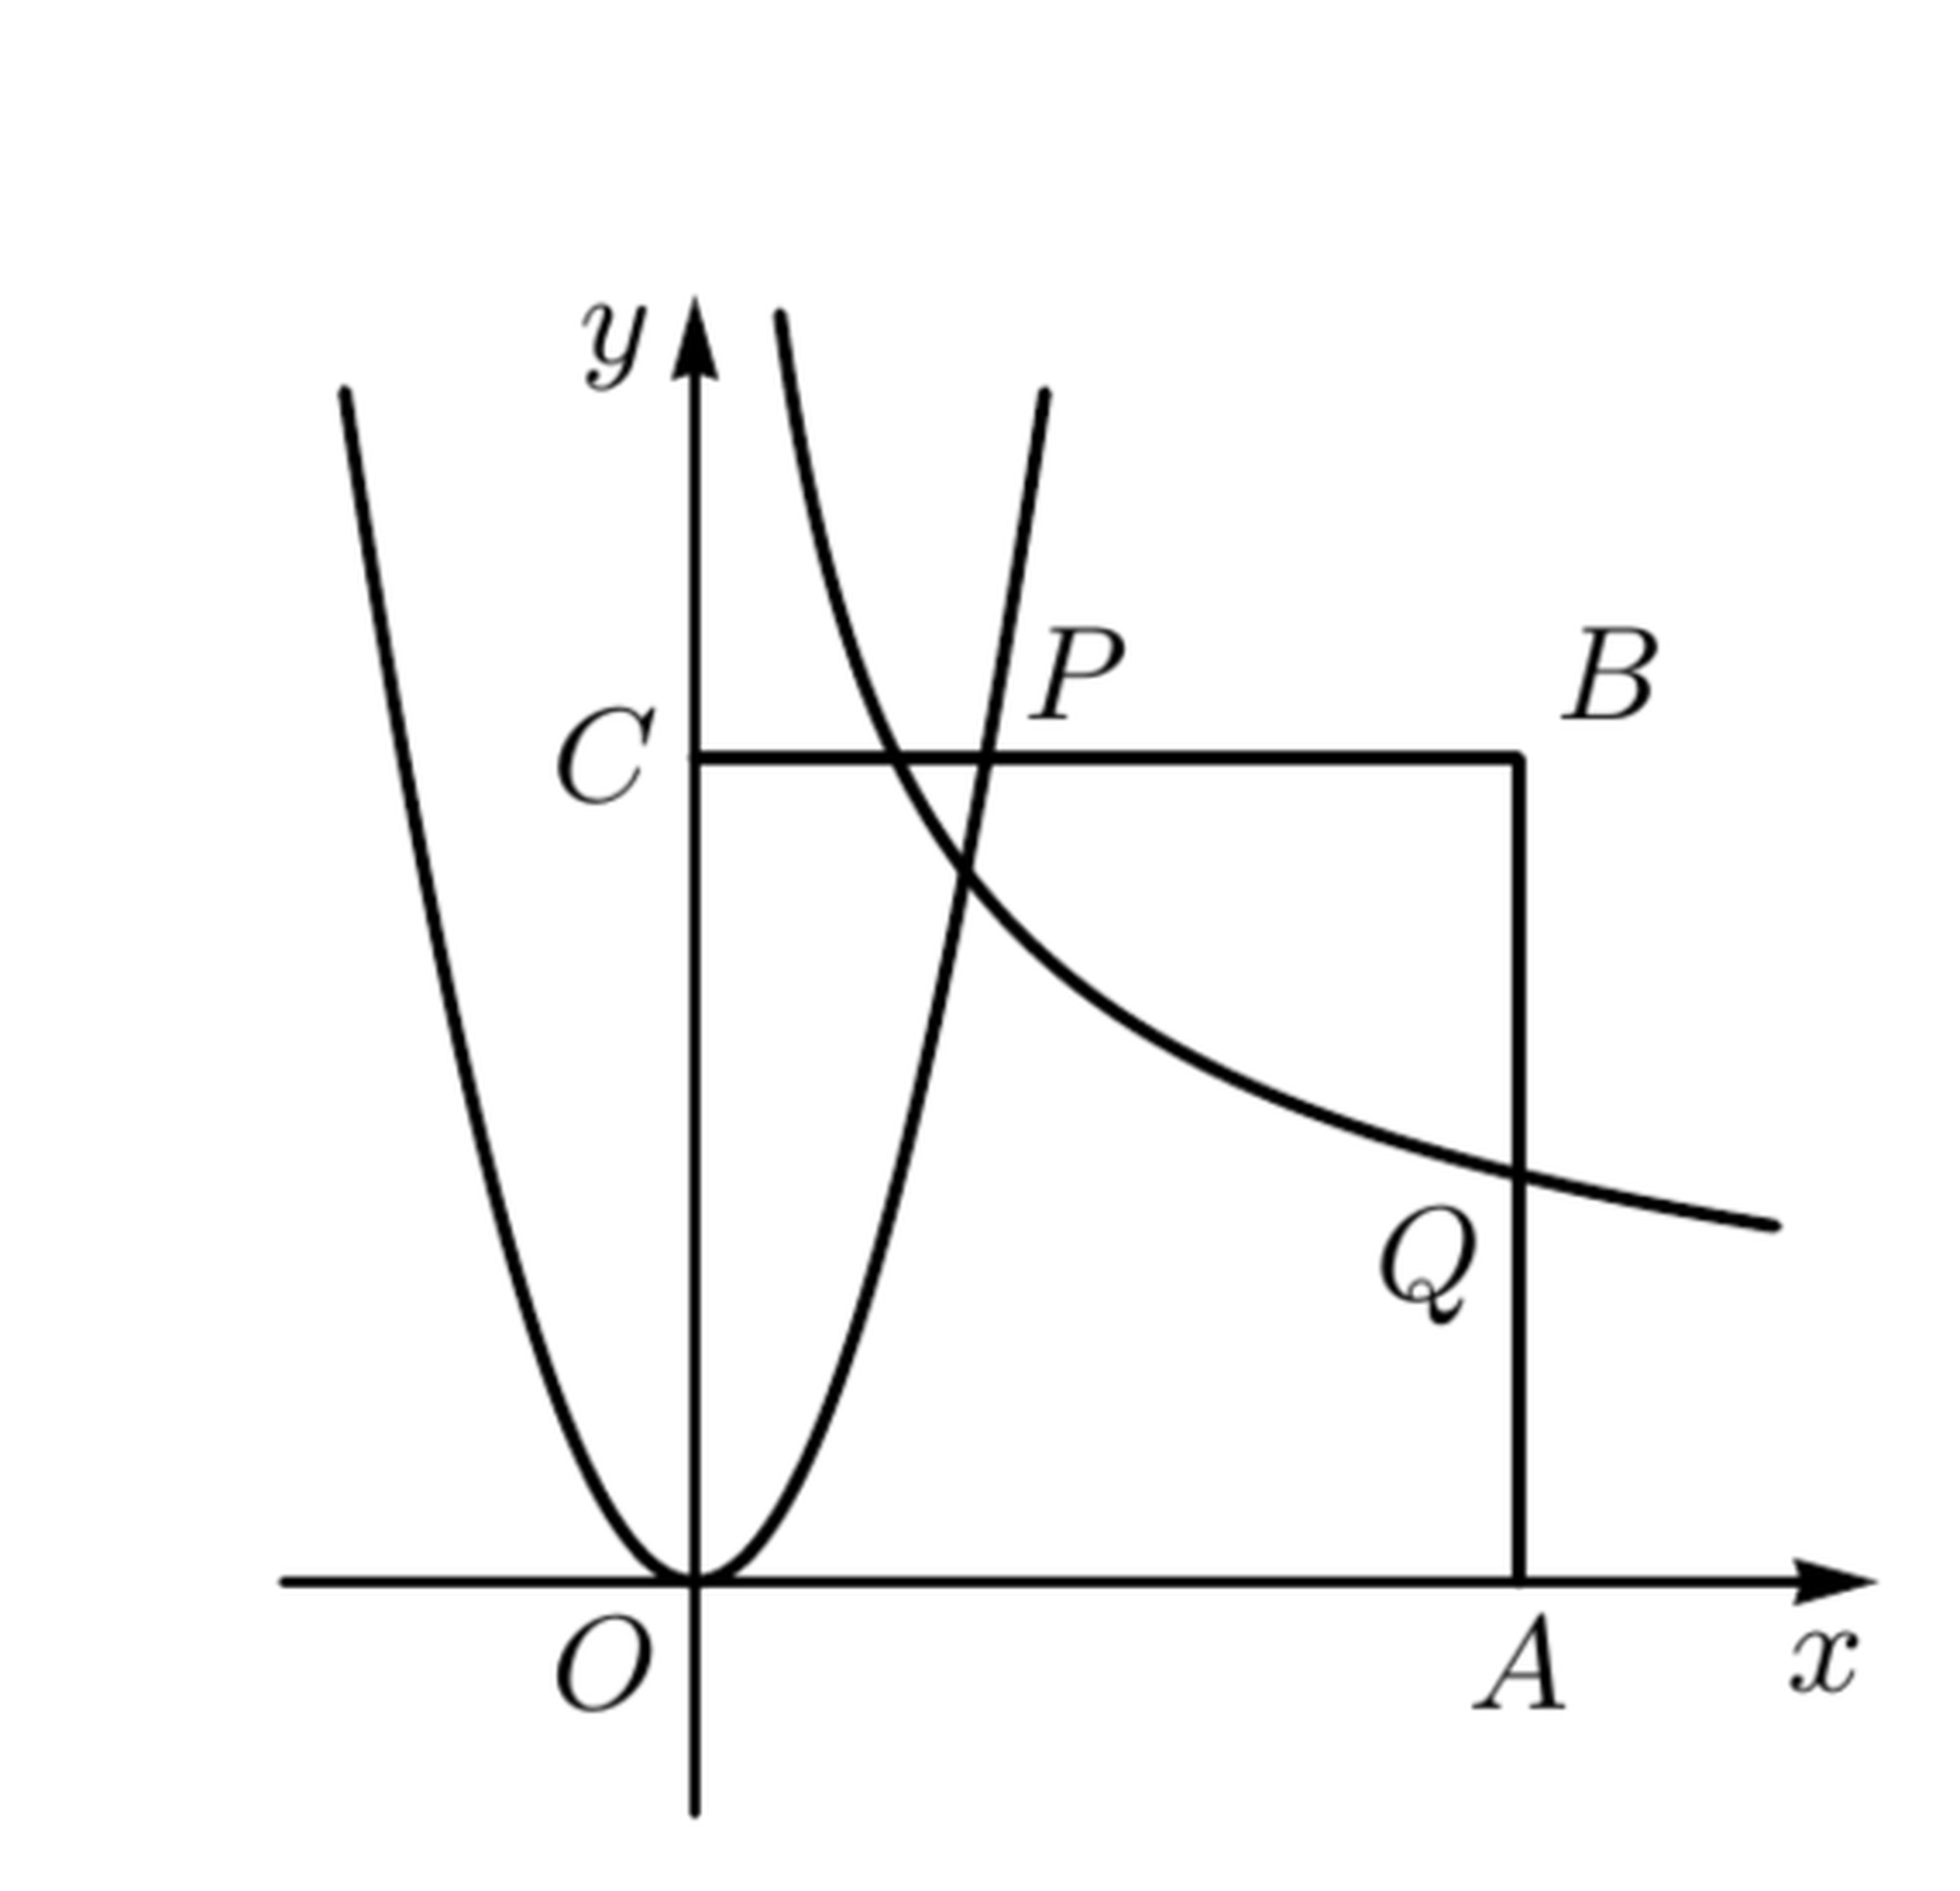
\includegraphics[width=0.40\textwidth]{figures/gao153_q11.png}
\end{center}

\ifanswer
\solbegin
\step{$\lvert AQ\rvert=\dfrac1{\sqrt a}$，$\lvert CP\rvert=\sqrt{\dfrac a5}$，}
\step{于是 $\lvert AQ\rvert+\lvert CP\rvert=\dfrac1{\sqrt a}+\sqrt{\dfrac a5}\geqslant2\sqrt{\dfrac1{\sqrt a}\cdot\sqrt{\dfrac a5}}=\dfrac2{\sqrt[4]{5}}$，}
\step{当且仅当 $\dfrac1{\sqrt a}=\sqrt{\dfrac a5}$，即 $a=\sqrt5$ 时取等号.}
\solend
\fi

% === Q12 === $B\subseteq A$ 带下划线照录、空集 \varnothing；解析 5 行
\item 若集合 $A=\{x\mid1\leqslant x\leqslant100,x\in\Z\}$，集合 $B\subseteq A$，且 $B\ne\varnothing$，记 $W(B)$ 为 $B$ 中元素的最大值与最小值之和，则对所有的 $B$，$W(B)$ 的平均值是\blankline[4.4em].

\ifanswer
\solbegin
\step{对每个非空子集 $B$，令 $B'=\{101-x\mid x\in B\}$，}
\step{则 $W(B')=(101-\min B)+(101-\max B)=202-W(B)$.}
\step{对 $B'$ 再作同样变换即得到 $B$，因此 $B$ 遍历所有非空子集时，}
\step{$B'$ 也恰好遍历所有非空子集.}
\step{设所求平均值为 $m$，则 $m=202-m$，解得 $m=101$.}
\solend
\fi

\end{enumerate}

\bigsec{二、选择题}

\begin{enumerate}
\setcounter{enumi}{12}

% === Q13 === "图像"（像，有亻）照录；解析 2 行，故选 A
\item 设 $a$、$b$ 为常数，若 $0<a<1$，$b>1$，则函数 $y=a^x-b$ 的图像必定不经过\mbox{（\quad）}

\keepwithprev
A. 第一象限\qquad\qquad B. 第二象限\qquad\qquad C. 第三象限\qquad\qquad D. 第四象限

\ifanswer
\solbegin
\step{当 $x>0$ 时，$a^x<1<b$，所以 $y=a^x-b<0$，图像必定不经过第一象限，}
\step{故选 $A$.}
\solend
\fi

% === Q14 === $m\in\Z$、中文弯引号、"图像"照录；解析 3 行，故选 A
\item 已知 $m\in\Z$，则“$m=0$”是“幂函数 $y=x^{m^2-2m-1}$ 的图像与 $x$ 轴及 $y$ 轴均无交点，且关于原点成中心对称”的\mbox{（\quad）}

\keepwithprev
A. 充分不必要条件\qquad\qquad B. 必要不充分条件

C. 充要条件\qquad\qquad D. 既不充分也不必要条件

\ifanswer
\solbegin
\step{图像满足所述条件 $\Leftrightarrow m^2-2m-1$ 为负奇数 $\Leftrightarrow m=0$ 或 $m=2$.}
\step{$m=0$ 能推出所述条件，但所述条件不能推出 $m=0$，因此是充分不必要条件，}
\step{故选 $A$.}
\solend
\fi

% === Q15 === 四选项一行；解析 5 行（跨 03→04 页），故选 D
\item 设 $a>b>1$，$x>1$，则下列不等式正确的是\mbox{（\quad）}

\keepwithprev
A. $a^x<b^x$\qquad B. $x^a<x^b$\qquad C. $\log_a x>\log_b x$\qquad D. $\log_x a>\log_x b$

\ifanswer
\solbegin
\step{$x>1$，幂函数与指数函数的单调性给出 $a^x>b^x$，$x^a>x^b$，A、B 错误.}
\step{$\log_a x=\dfrac{\lg x}{\lg a}<\dfrac{\lg x}{\lg b}=\log_b x$，C 错误.}
\step{对数函数 $y=\log_x t$ 的底数 $x>1$，在 $(0,+\infty)$ 上严格递增，}
\step{所以 $\log_x a>\log_x b$，D 正确.}
\step{故选 $D$.}
\solend
\fi

% === Q16 === $a\in\N$；解析 3 行，故选 C
\item 设 $a\in\N$，则满足不等式 $x^2-a^2x-a^2-1<0$ 的整数 $x$ 的个数不可能是\mbox{（\quad）}

\keepwithprev
A. 1\qquad\qquad B. 50\qquad\qquad C. 100\qquad\qquad D. 2026

\ifanswer
\solbegin
\step{$(x+1)(x-a^2-1)<0\Leftrightarrow-1<x<a^2+1$. 整数解为 $0,1,\cdots,a^2$，共 $a^2+1$ 个.}
\step{$1=0^2+1$，$50=7^2+1$，$2026=45^2+1$，而 $100-1=99$ 不是完全平方数，}
\step{故选 $C$.}
\solend
\fi

\end{enumerate}

\bigsec{三、解答题}

\begin{enumerate}
\setcounter{enumi}{16}

% === Q17 === 补集上划线 \overline{A}、\subseteq 照录；解析 5 行
\item 已知全集 $U=\R$，集合 $A=\{x\mid x^2-x-2\geqslant0\}$，$B=\{x\mid x>-1\}$，$C=\{x\mid a-5<x<a\}$.

(1) 求 $A\cap B$、$A\cup B$；

(2) 若 $\overline{A}\cup C=C$，求实数 $a$ 的取值范围.

\ifanswer
\solbegin
\step{(1) $x^2-x-2=(x+1)(x-2)\geqslant0\Leftrightarrow x\leqslant-1$ 或 $x\geqslant2$，}
\step{所以 $A=(-\infty,-1]\cup[2,+\infty)$，$B=(-1,+\infty)$，}
\step{因此 $A\cap B=[2,+\infty)$，$A\cup B=\R$.}
\step{(2) $\overline{A}=(-1,2)$，于是 $\overline{A}\cup C=C\Leftrightarrow\overline{A}\subseteq C\Leftrightarrow(-1,2)\subseteq(a-5,a)$，}
\step{两区间均为开区间，端点可重合，故 $\begin{cases}a-5\leqslant-1\\a\geqslant2\end{cases}\Leftrightarrow2\leqslant a\leqslant4$.}
\solend
\fi

% === Q18 === 解析 4 行
\item 已知 $a$、$b$、$c$ 都是正数，

(1) 若 $a+b=1$，求证：$\dfrac1a+\dfrac1b\geqslant4$，并指出等号成立的条件；

(2) 若 $a+b+c=1$，求证：三个数 $\dfrac1a$、$\dfrac1b$、$\dfrac1c$ 中至少有一个不小于 3.

\ifanswer
\solbegin
\step{(1) 由 $(a-b)^2\geqslant0$，得 $4ab\leqslant(a+b)^2=1$，所以 $\dfrac1a+\dfrac1b=\dfrac{a+b}{ab}=\dfrac1{ab}\geqslant4$，}
\step{等号成立当且仅当 $a=b$，结合 $a+b=1$，得 $a=b=\dfrac12$.}
\step{(2) 假设三个数 $\dfrac1a$、$\dfrac1b$、$\dfrac1c$ 都小于 3，则 $a>\dfrac13,b>\dfrac13,c>\dfrac13\Rightarrow a+b+c>1$，}
\step{与 $a+b+c=1$ 矛盾，因此三个数中至少有一个不小于 3.}
\solend
\fi

% === Q19 === 题目配图（三版都出）；\needvspace 守卫放 \item 之前；解析 19 行
\needvspace{8cm}
\item 某新建居民小区有一直角三角形绿地，两直角边长分别为 30m 和 40m，打算在其中划出一片区域改造成活动场地，如图所示.

(1) 若划出的区域为正方形，且有两边落在绿地边界上，求此正方形边长；

(2) 若划出的区域为圆形，求圆形区域面积的最大值；

(3) 若划出的区域为矩形（其中至少有一边在边界上），求此矩形面积的最大值.

\begin{center}
% 直角三角形 ABC 绿地示意图取 05 页右上，去粉色水印、去色、4× LANCZOS 放大；三版都出
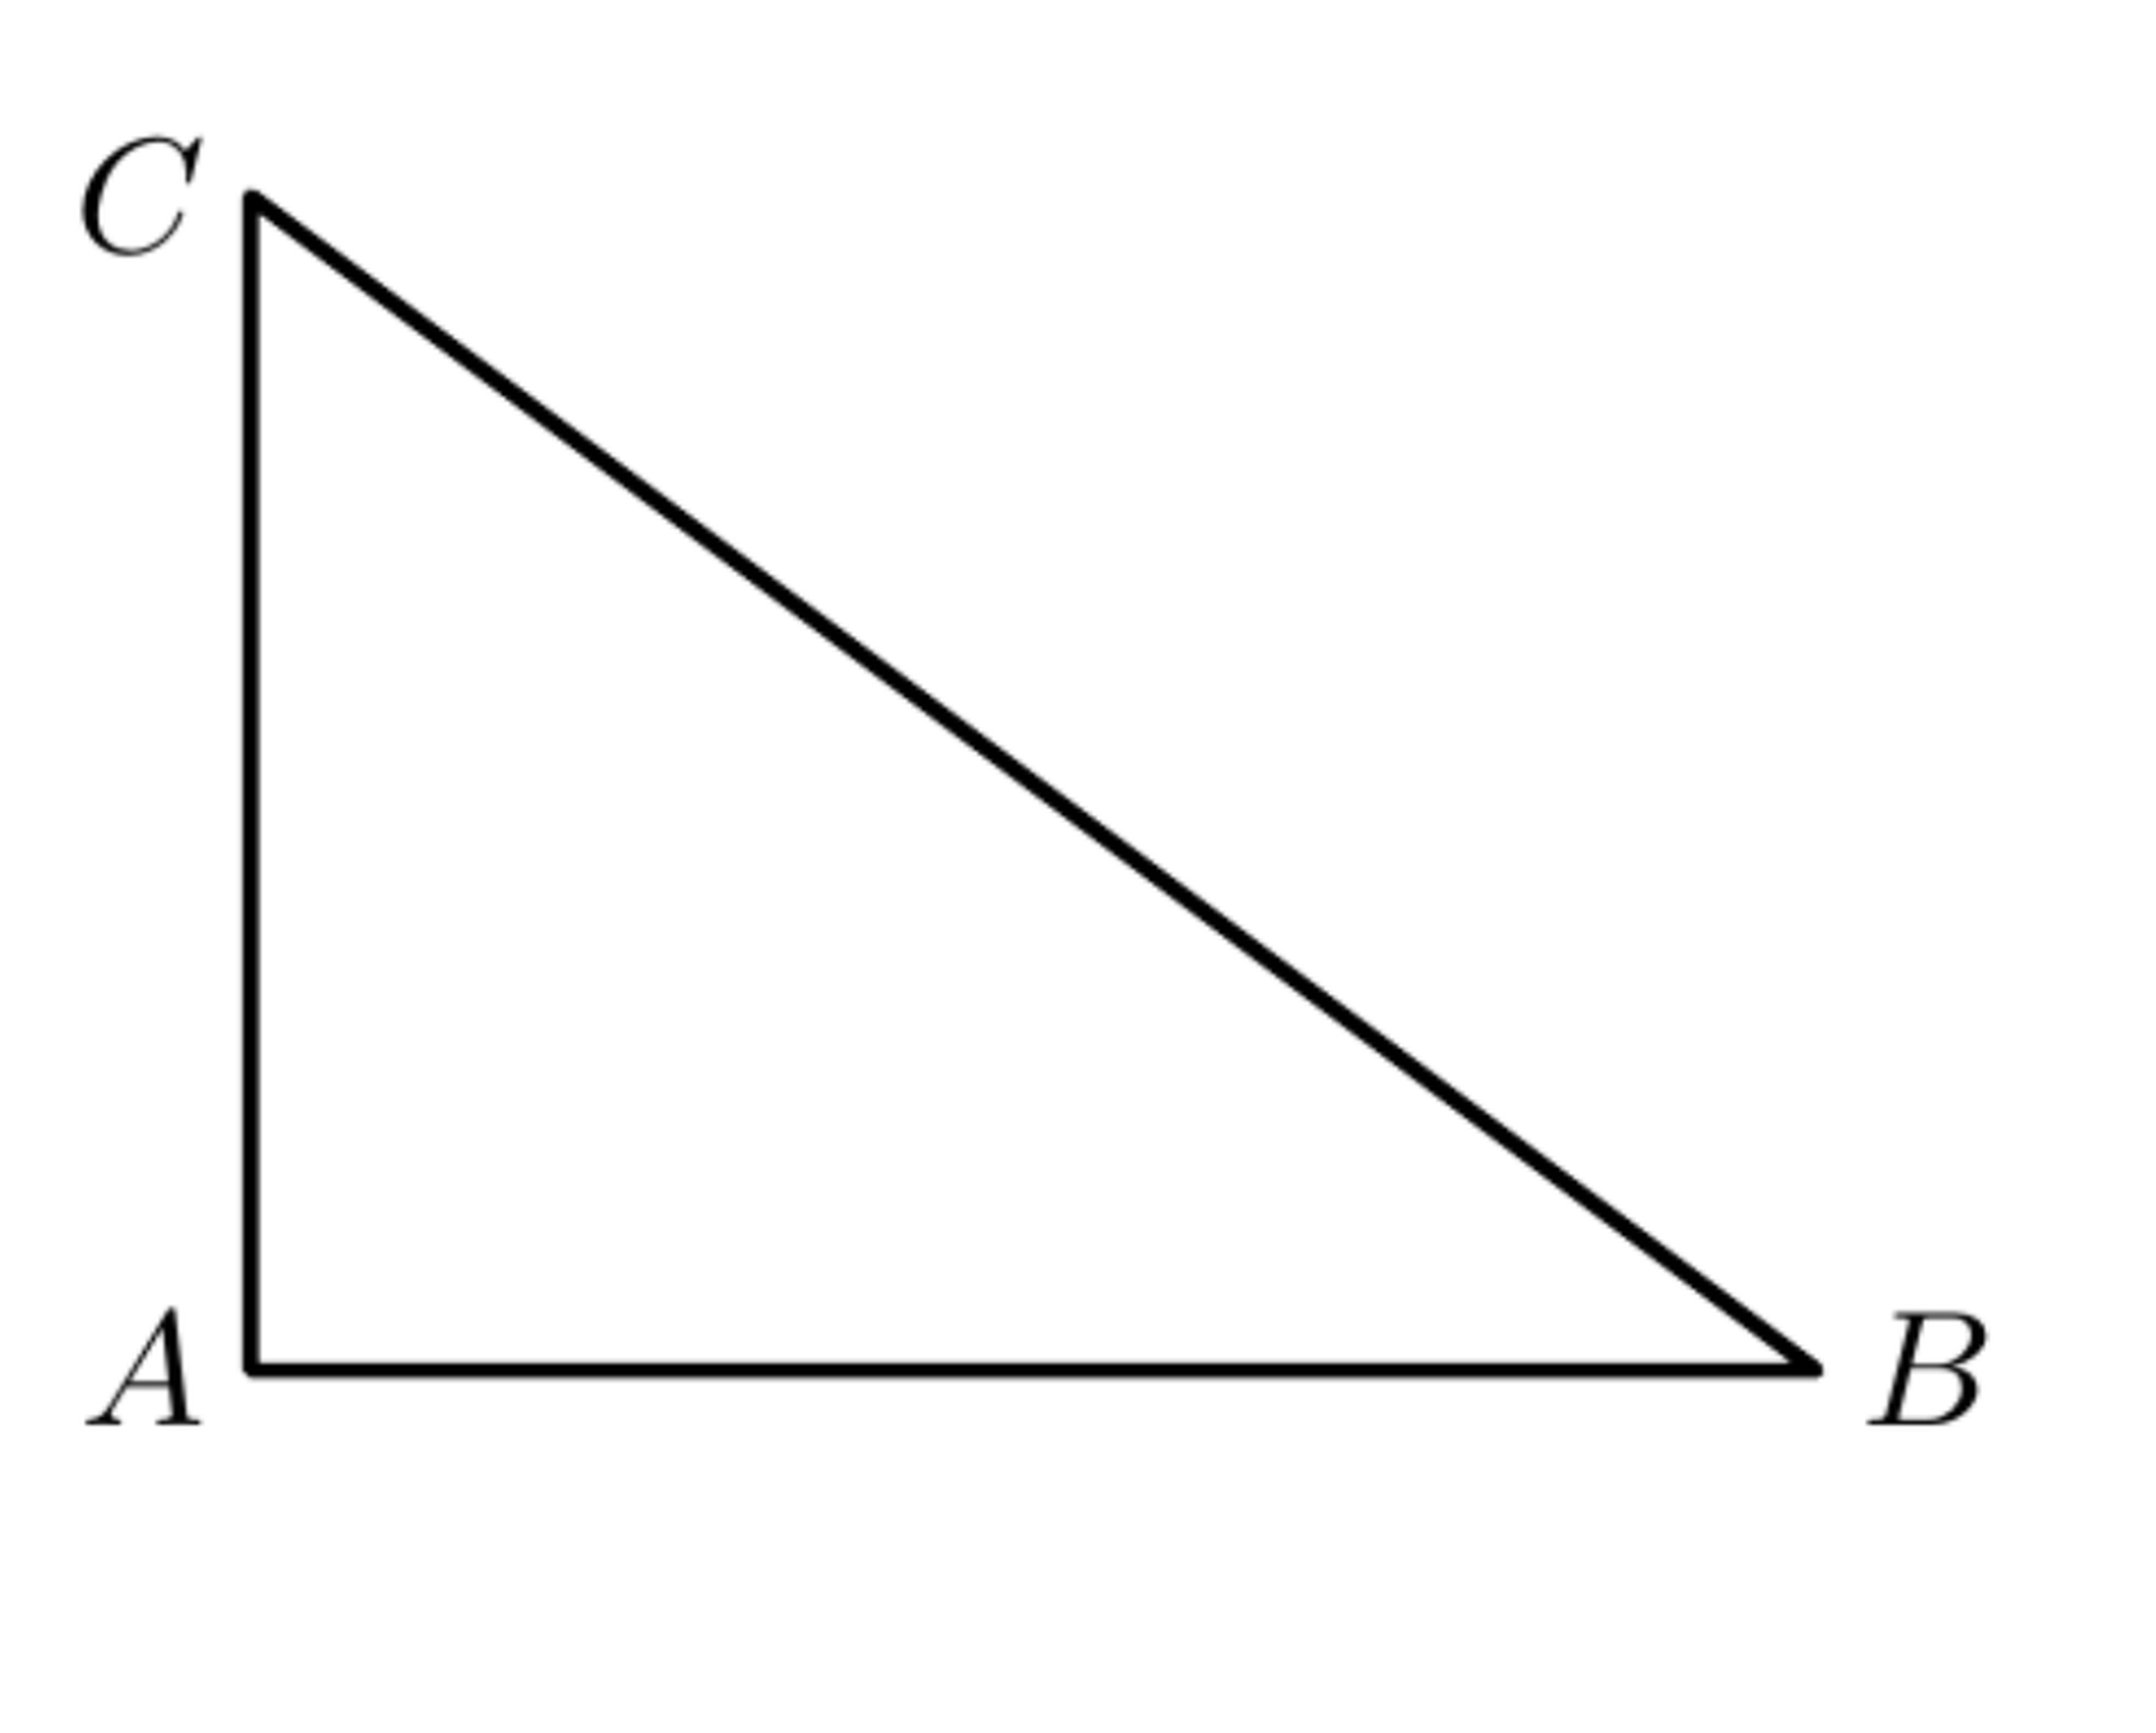
\includegraphics[width=0.34\textwidth]{figures/gao153_q19.png}
\end{center}

\ifanswer
\solbegin
\step{(1) 取 $A(0,0)$、$B(40,0)$、$C(0,30)$，则斜边 $BC$ 所在直线为 $3x+4y=120$.}
\step{正方形落在边界上的两边必分别在两条直角边上.}
\step{设其边长为 $a$m，则对角顶点为 $(a,a)$.}
\step{按题意划出的正方形应尽量大，即对角顶点落在斜边 $BC$ 上，}
\step{因此 $3a+4a=120\Rightarrow a=\dfrac{120}{7}$；}
\step{(2) 斜边长 $BC=\sqrt{30^2+40^2}=50$m，三角形面积为 $600\text{m}^2$.}
\step{设圆的半径为 $r$，圆心到 $AB$、$AC$、$BC$ 的距离分别为 $d_1,d_2,d_3$，}
\step{则三者均不小于 $r$. 连接圆心与三个顶点，}
\step{得 $600=\dfrac12(40d_1+30d_2+50d_3)\geqslant\dfrac12(40+30+50)r=60r$，所以 $r\leqslant10$.}
\step{取三角形的内切圆时等号成立，圆形区域面积的最大值为 $100\pi\text{m}^2$.}
\step{(3) 任取矩形落在绿地边界上的一边，以其所在直线为横轴.}
\step{设相应三角形底边长为 $L$、高为 $H$，则 $LH=1200$.}
\step{取三角形顶点坐标为 $(0,0)$、$(L,0)$、$(p,H)$.}
\step{在高度 $t$ 处，两腰上的点的横坐标分别为 $\dfrac{pt}{H}$、$L+\dfrac{(p-L)t}{H}$，}
\step{因此，高为 $t$ 的矩形，其底边长不超过 $L\left(1-\dfrac tH\right)$，}
\step{面积满足 $S\leqslant Lt\left(1-\dfrac tH\right)=\dfrac LH\left[\dfrac{H^2}{4}-\left(t-\dfrac H2\right)^2\right]\leqslant\dfrac{LH}{4}=300$，}
\step{在原坐标系中，取矩形顶点为 $(0,0)$、$(20,0)$、$(20,15)$、$(0,15)$，}
\step{其中 $3\times20+4\times15=120$，矩形完全位于绿地内，面积为 $300\text{m}^2$，}
\step{达到最大值.}
\solend
\fi

% === Q20 === $g(x)$ 定义照录；解析 14 行
\item 已知 $a>0$ 且 $a\ne1$，设 $f(x)=\log_a(x^2-a^2)$，$g(x)=2\log_a(x-ak)$.

(1) 求函数 $y=f(x)$ 的定义域；

(2) 若 $k=2$，求不等式 $f(x)>g(x)$ 的解集；

(3) 若“存在实数 $x$，使得 $f(x)=g(x)$”为真命题，求实数 $k$ 的取值范围.

\ifanswer
\solbegin
\step{(1) $x^2-a^2>0\Leftrightarrow x<-a$ 或 $x>a$，定义域为 $(-\infty,-a)\cup(a,+\infty)$.}
\step{(2) 两函数均有意义时，$x>2a$，且 $g(x)=\log_a(x-2a)^2$.}
\step{当 $a>1$ 时，$f(x)>g(x)\Leftrightarrow x^2-a^2>(x-2a)^2\Leftrightarrow x>\dfrac{5a}{4}$，}
\step{结合 $x>2a$，解集为 $(2a,+\infty)$.}
\step{当 $0<a<1$ 时，$f(x)>g(x)\Leftrightarrow x^2-a^2<(x-2a)^2\Leftrightarrow x<\dfrac{5a}{4}$，}
\step{与 $x>2a$ 矛盾，解集为 $\varnothing$.}
\step{(3) 在 $x^2-a^2>0$ 且 $x-ak>0$ 的条件下，}
\step{$f(x)=g(x)\Leftrightarrow x^2-a^2=(x-ak)^2\Leftrightarrow2akx=a^2(1+k^2)$，}
\step{当 $k=0$ 时，上式不成立；}
\step{当 $k\ne0$ 时，$x=\dfrac{a(1+k^2)}{2k}$，}
\step{于是 $x-ak=\dfrac{a(1-k^2)}{2k}>0\Leftrightarrow k<-1$ 或 $0<k<1$，}
\step{对上述 $k$，所取的 $x$ 同时满足 $x^2-a^2=(x-ak)^2>0$，}
\step{两函数均有意义且函数值相等.}
\step{因此，$k$ 的取值范围为 $(-\infty,-1)\cup(0,1)$.}
\solend
\fi

% === Q21 === 中文弯引号、复杂式照录；解析 23 行（跨 08→09 页）
\item 若实数 $x$、$y$、$m$ 满足 $\lvert x-m\rvert<\lvert y-m\rvert$，则称 $x$ 比 $y$ 接近 $m$.

(1) 若 $2x$ 比 $x-2$ 更接近 1，求实数 $x$ 的取值范围；

(2) 若 $x$ 比 $y$ 接近 $m$，证明：“$x>y$” 的充要条件是 “$x+y<2m$”；

(3) 已知 $x>0$，$y>0$ 且 $x\ne y$. 设 $p=\dfrac{x^2+y^2}{xy}$，若对于任意的 $x$、$y$，命题 “$p$ 比 $p^2-3p+4$ 接近 $m$” 恒成立，求实数 $m$ 的取值范围.

\ifanswer
\solbegin
\step{(1) $\lvert2x-1\rvert<\lvert x-3\rvert\Leftrightarrow(2x-1)^2<(x-3)^2\Leftrightarrow(x+2)(3x-4)<0$，}
\step{解得 $-2<x<\dfrac43$，实数 $x$ 的取值范围为 $\left(-2,\dfrac43\right)$.}
\step{(2) 因为 $x$ 比 $y$ 接近 $m$，所以 $\lvert x-m\rvert<\lvert y-m\rvert$，则 $\lvert x-m\rvert^2<\lvert y-m\rvert^2$，}
\step{即 $(x-m)^2<(y-m)^2$，即 $(x-m)^2-(y-m)^2<0$，}
\step{即得 $(x-y)(x+y-2m)<0$，}
\step{则由 $x+y<2m$，得 $x+y-2m<0$，}
\step{故 $x-y>0$，即 $x>y$，充分性成立；}
\step{当 $x>y$ 时，$x-y>0$，结合 $(x-y)(x+y-2m)<0$，得 $x+y-2m<0$，}
\step{即 $x+y<2m$，必要性成立；}
\step{故“$x>y$” 的充要条件是 “$x+y<2m$”；}
\step{(3) $x>0$，$y>0$ 且 $x\ne y$. 则 $p=\dfrac{x^2+y^2}{xy}=\dfrac xy+\dfrac yx>2\sqrt{\dfrac xy\cdot\dfrac yx}=2$，}
\step{由于对于任意的 $x$、$y$，命题 “$p$ 比 $p^2-3p+4$ 接近 $m$” 恒成立，}
\step{故 $\lvert p-m\rvert<\lvert(p^2-3p+4)-m\rvert$ 对 $\forall p>2$ 恒成立，}
\step{即得 $(p-m)^2<(p^2-3p+4-m)^2$，}
\step{即 $(p^2-3p+4-m)^2-(p-m)^2>0$，}
\step{得 $(p^2-4p+4)(p^2-2p+4-2m)>0$，}
\step{即 $(p-2)^2(p^2-2p+4-2m)>0$，由于 $p>2$，故 $(p-2)^2>0$，}
\step{故 $p^2-2p+4-2m>0$ 对 $\forall p>2$ 恒成立，}
\step{即 $2m<p^2-2p+4$ 对 $\forall p>2$ 恒成立，}
\step{由于 $p^2-2p+4=(p-1)^2+3$，此时 $p^2-2p+4$ 在 $(2,+\infty)$ 上严格增，}
\step{故 $(p-1)^2+3>(2-1)^2+3=4$，故 $2m\leqslant4$，解得 $m\leqslant2$，}
\step{即实数 $m$ 的取值范围是 $(-\infty,2]$.}
\solend
\fi

\end{enumerate}

\end{document}
"
% 紧凑版：xelatex "\def\iscompact{1}% 高一153_闵行中学文绮中学_期中.tex
%   —— 高一上数学"2026-2027 年闵行中学文绮中学高一上期中"（试卷版/答案版/紧凑版）
% 试卷版：xelatex 高一153_闵行中学文绮中学_期中.tex
% 答案版：xelatex "\def\isanswer{1}% 高一153_闵行中学文绮中学_期中.tex
%   —— 高一上数学"2026-2027 年闵行中学文绮中学高一上期中"（试卷版/答案版/紧凑版）
% 试卷版：xelatex 高一153_闵行中学文绮中学_期中.tex
% 答案版：xelatex "\def\isanswer{1}\input{高一153_闵行中学文绮中学_期中.tex}"
% 紧凑版：xelatex "\def\iscompact{1}\input{高一153_闵行中学文绮中学_期中.tex}"
%
% ① 原始材料：微信公众号"魔都数学加油站"文章，连载"27学年高一153"，原文标题
% "27学年高一153——2026-2027年上海市闵行中学文绮中学高一上期中"；
% 原文链接：https://mp.weixin.qq.com/s/rEtS-92cDR6JKgY2b5DRfg 。
% 正文为 9 张 PNG 页（01/02/06/07/08/09 为 2560×3620，03/04/05 为 4762×6735，
% 同一篇各页分辨率混排，逐页按各自分辨率裁图核对，别按预览比例换算裁框）。
% 体例：讲评版——填空 3—12（10 题）、选择 13—16（4 题）、解答 17—21（5 题），
% 共 19 题，自第 3 题起编；**全 19 题均印【解析】**（逐题核实，见 ② ②）。
% 题目、答案、解析均据原图转录；卷面粉红色水印"魔都数学加油站"及公众号页脚未录入。
% 全卷插图清单（逐页通读 9 页确认）：2 幅，均为题目配图、三版都出——
%   · Q11 正方形 OABC 曲线图（02 页右下：$y=5x^2$ 与 $y=x^{-\frac12}$ 两条曲线、
%     坐标轴、O/A/B/C/P/Q、正方形），裁 figures/gao153_q11.png；
%   · Q19 直角三角形 ABC 绿地示意图（05 页右上，直角在 A），
%     裁 figures/gao153_q19.png；
%   两图均去粉色水印、去色、4× LANCZOS 放大；Q11 图左上角题干残字"函"已裁白。
%   其余各页逐页确认无其它题目配图、无解析内配图、无表格；09 页下半仅水印、无正文。
%
% 卷首标题：原卷印作"2026-2027 年闵行中学文绮中学高一上期中"，年份区间按全稿惯例排 en dash；
% 原卷卷面未印副标题，本稿按同期中卷知识模块口径补出"集合与常用逻辑用语、不等式、函数"。
%
% ② 与原卷的排版差异：
%   ① 原文从第 3 题起，本稿保留原题号；共 19 题三节，解答题 5 题到 21；
%   ② 全 19 题均印【解析】、用 \solbegin…\solend，无只印【答案】或答案印括号内的题；
%      四道选择题答案在解析末句"故选 A／A／D／C"（Q13—Q16，逐个放大复核）、
%      括号 \mbox{（\quad）} 留空、不另提 \ans{}；答案版【答案】/【解析】标记数
%      = 19 = 全卷题数；
%   ③ 原卷卷面未印副标题，本稿按知识模块口径补出；
%   ④ 原卷填空横线按全稿惯例排 \blankline[4.4em]；选择题括号排 \mbox{（\quad）}、
%      四道选择题的选项段前按惯例各加 \keepwithprev；解答题不留作答区、不加
%      \anspace（原卷为讲评版，109—113 起全稿不用 \anspace）；
%   ⑤ 数集：Q3"$x\in R$"、Q5"解集为 R"、Q10"$x\in N$"、Q12"$x\in Z$"与
%      "$m\in Z$"、Q14"$m\in Z$"、Q16"$a\in N$"、Q17"全集 $U=R$"、
%      Q19 无、Q21 无——原卷印斜体或正体粗体 R/N/Z，按全稿惯例归一
%      \R／\N／\Z；绝对值排 \lvert…\rvert（Q5、Q11、Q21），集合描述竖线排 \mid
%      （Q3、Q10、Q17、Q20），不等号按全稿惯例排 \leqslant／\geqslant；
%      补集照原卷上划线排 \overline{A}（Q17 题干 (2)＋解析 (2)）；
%      空集 \varnothing（Q12 题干、Q20 解析 (2)）；子集 3 处均印带下划线 ⊆、
%      照录 \subseteq（Q10 $A\subseteq U$、Q12 $B\subseteq A$、Q17 $(-1,2)\subseteq(a-5,a)$），
%      本卷无单线 \subset 用例；
%   ⑥ 判别式：逐页通读 9 页，本卷无一元二次判别式 Δ/△ 算式，故无 Δ/△ 混用可照录；
%      Q11 图里有几何正方形 OABC（非三角形符号），无 △ABC 用例；
%   ⑦ 中文弯引号照录：Q14"$m=0$"与"幂函数…关于原点成中心对称"、
%      Q20"存在实数 $x$，使得 $f(x)=g(x)$"、Q21"$x>y$"与"$x+y<2m$"、
%      "$p$ 比 $p^2-3p+4$ 接近 $m$"（引号外留空格按原卷）；
%      注释里一律 ASCII 引号；数学式内 CJK 用 \text{}；
%   ⑧ "图像／图象"逐处放大核：全卷 3 处均印"图像"（像，有亻）——
%      Q13 题干与解析、Q14 题干与解析；Q19 题干写"如图所示"（非"图像"），
%      逐处照录未统一；子题标号 (1)(2)(3) 半角括号照录；圈数字本卷无用例；
%   ⑨ 半角逗号在数学组之间是全稿惯例、非笔误，逐处照录（Q3 $x\in R$、
%      Q10 $a_1,a_2$、Q19 $A(0,0)$、$d_1,d_2,d_3$、Q21 $a>\frac13,b>\frac13$ 等）；
%      行末西文句点 ASCII `.`；行中全角逗号／顿号照录（Q19"30m 和 40m"、
%      Q21"实数 $x$、$y$、$m$"）；
%   ⑩ 复杂式照录别简化：Q3 $y=x^{-2}$、Q11 $y=x^{-\frac12}$ 与
%      $\frac{2}{\sqrt[4]{5}}$、Q8 $\frac{2b}{a+1-b}$、Q9 cases 块、
%      Q10 $525=5\times105$、Q16 $a^2+1$、Q19 $S\leqslant Lt(1-\frac tH)$
%      与 $L+\frac{(p-L)t}{H}$、Q20 $2akx=a^2(1+k^2)$ 与 $\frac{a(1+k^2)}{2k}$、
%      Q21 $(p^2-4p+4)(p^2-2p+4-2m)>0$；
%      \left…\right 不得拆到不同 $…$ 组（Q17 $\left\{x\mid\cdots\right\}$、
%      Q19 $\left[\frac{H^2}{4}-\left(t-\frac H2\right)^2\right]$、
%      Q21 $\left(-2,\frac43\right)$ 等）；cases 块一律 \begin{cases}…\end{cases}；
%   ⑪ 一条 \step = 原卷解析的一个印刷行，cases 块整体算一个印刷行；别并折行、
%      别拆行。Q10 六行、Q19 十九行、Q20 十四行、Q21 二十二行均按印刷行逐条断，
%      不丢行；
%   ⑫ 配图：Q11／Q19 题目配图（三版都出）放 \item 内题干之后 \begin{center}，
%      各用 \needvspace{8cm} 守卫把整块推走，**守卫放在 \item 之前**
%      （见 高一145 Q14/Q20 成例与切页审计 B 类坑）；
%   ⑬ 原卷解析内无红色"法一／法二"之类小标题，故本卷无 \stepm；红色水印
%      "魔都数学加油站"不录入；
%   ⑭ 跨页续印按题合并：见 ⑥；
%
% ③ 行数复核：一条 \step = 原卷解析的一个印刷行，cases 块作一个印刷行计。
%   逐题数（主会话逐页核对定稿）：Q3：1；Q4：2；Q5：2；Q6：2；Q7：1；
%   Q8：1；Q9：2；Q10：6；Q11：3；Q12：5；Q13：2；Q14：3；Q15：5；
%   Q16：3；Q17：5；Q18：4；Q19：19；Q20：14；Q21：22。
%   合计 102 条 \step（本卷无 \stepm），与原卷逐题印刷行相等。全卷 19 题
%   均设 \solbegin…\solend，答案版【答案】/【解析】标记数 = 19 = 全卷题数。
%
% ④ 判别式／子集符号结论（逐处放大原图照录、不得统一，主会话像素级复核）：
%   判别式：逐页通读 9 页，本卷无一元二次判别式算式（Q7 用韦达定理、
%      Q16 用因式分解、Q20 用对数方程，均不写 Δ/△），故无 Δ/△ 混用可照录
%      （"高 \Delta／扁 \triangle"口径备查，参照 高一142／151／152 头注）；
%      本卷无几何三角形符号用例。
%   子集：Q10 题干"$A\subseteq U$"、Q12 题干"$B\subseteq A$"、Q17 解析 (2)
%      "$(-1,2)\subseteq(a-5,a)$"共 3 处，逐处放大确认均印带下划线 ⊆、
%      照录 \subseteq；本卷未见单线 ⊂（\subset）之对应处。
%      补集上划线 \overline{A}（Q17）、空集 \varnothing（Q12 题干、Q20 解析 (2)）；
%      数集 \R／\N／\Z 归一见 ② ⑤。
%
% ⑤ 存疑照录（放大原图确认，照录未改、正文对应处另有 % 注）：
%   1. Q3 集合 $B=\{(x,y)\mid y=x^{-2},x\in\R\}$ 原卷题干径写 $x\in\R$
%      （$x=0$ 处无意义），解析自行注明 $x\ne0$，照录未改。
%   2. Q10 解析"$U$ 中共有 $525=5\times105$ 个连续整数"与尾行
%      "取 $U$ 中除以 5 余 1 或 2 的全部元素及元素 5"逐字照录（放大 02 页
%      /tmp/gao153/z/zoom/q10_pick.png 确认是"元素 5"，非"元素 9"）。
%   3. Q11 第二个函数原卷印 $y=x^{-\frac12}$（负二分之一次幂，非 $x^2$），
%      放大 02 页 /tmp/gao153/z/zoom/q11_exp.png 确认，照录未改；
%      $|AQ|=\frac1{\sqrt a}$ 与之自洽。
%   4. Q19 (3) 解析"在高度 $t$ 处，两腰上的点的横坐标分别为 $\frac{pt}{H}$、
%      $L+\frac{(p-L)t}{H}$"，放大 06 页确认，照录未简化。
%   5. Q20 (2) 解析"$g(x)=\log_a(x-2a)^2$"（真数整体平方），
%      与 $g(x)=2\log_a(x-ak)$ 在 $k=2$ 时一致，照录未改。
%   6. Q21 (3) 解析"得 $(p^2-4p+4)(p^2-2p+4-2m)>0$"与
%      "故 $(p-1)^2+3>(2-1)^2+3=4$，故 $2m\leqslant4$"照录未改
%      （放大 09 页 /tmp/gao153/z/zoom/q21_factor.png 确认）。
%   7. "图像／图象"全卷 3 处均印"图像"（像，有亻）逐处照录；
%      本卷无判别式 Δ/△ 用例（见 ④）。
%   全卷除此 7 类外未发现其它笔误／自相矛盾处；19 题均印【解析】、
%   无只印【答案】或答案印括号内的题（见 ② ②）。
%
% ⑥ 跨页续印按题合并说明（逐页核实定稿）：Q3—Q5 题干＋解析在 01 页；
%   Q6—Q8 题干＋解析在 01 页下半（Q8 解析续 02 页顶）；Q9 题干＋解析、
%   Q10 题干＋解析首 2 行在 02 页上半，Q10 解析余 4 行在 02 页下半；
%   Q11 题干＋配图＋解析、Q12 题干＋解析 5 行在 02 页下半—03 页上半；
%   "二、选择题"标题在 03 页中部；Q13 题干＋选项＋解析在 03 页下半；
%   Q14 题干＋选项＋解析、Q15 题干＋选项＋解析首行在 03 页下半—04 页顶；
%   Q15 解析余 4 行、Q16 题干＋选项＋解析在 04 页上半；"三、解答题"
%   标题在 04 页下半；Q17 题干＋两问＋解析 5 行在 04 页下半—05 页顶；
%   Q18 题干＋两问＋解析 4 行、Q19 题干（含配图）＋三问在 05 页；
%   Q19 解析 (1)(2) 9 行在 05 页下半，解析 (3) 前 5 行在 06 页上半、
%   余 4 行在 06 页下半；Q20 题干＋三问在 06 页下半，解析 (1)(2)(3)
%   前 6 行在 07 页上半、(3) 余 8 行在 07 页下半；Q21 题干＋三问在
%   07 页末，解析 (1)(2) 10 行在 08 页上半—下半，解析 (3) 前 4 行在
%   08 页下半、余 9 行续 09 页上半，末行"即实数 $m$ 的取值范围是
%   $(-\infty,2]$"为全卷收尾（09 页下半仅水印、无正文）。
%   本稿按题连排，不丢行、不并折行；全卷末题为第 21 题，无附加题节。
%
\documentclass[a4paper,11pt]{article}
\usepackage{common}

\begin{document}

\examtitlest[3]{2026--2027 年闵行中学文绮中学高一上期中}{集合与常用逻辑用语、不等式、函数}

\bigsec{一、填空题}

\begin{enumerate}
\setcounter{enumi}{2}

% === Q3 === 集合描述竖线 \mid；$y=x^{-2}$ 照录；解析 1 行
\item 已知 $A=\{(x,y)\mid y=x^3,x\in\R\}$，$B=\{(x,y)\mid y=x^{-2},x\in\R\}$，则 $A\cap B=$\blankline[4.4em].

\ifanswer
\solbegin
\step{$x^3=x^{-2}\ (x\ne0)\Leftrightarrow x^5=1\Leftrightarrow x=1$，此时 $y=1$，所以 $A\cap B=\{(1,1)\}$.}
\solend
\fi

% === Q4 === 解析 2 行
\item 若关于 $x$ 的不等式 $\dfrac{x-a}{x+1}>0$ 的解集为 $(-\infty,-1)\cup(4,+\infty)$，则实数 $a=$\blankline[4.4em].

\ifanswer
\solbegin
\step{关于 $x$ 的不等式 $\dfrac{x-a}{x+1}>0$ 即 $(x+1)(x-a)>0$.}
\step{再由它的解集为 $(-\infty,-1)\cup(4,+\infty)$，得 $-1$ 和 4 是 $(x+1)(x-a)=0$ 的两个实数根，故 $a=4$.}
\solend
\fi

% === Q5 === 绝对值 \lvert…\rvert；解析 2 行
\item 若关于 $x$ 的不等式 $\lvert x+1\rvert+\lvert x-2\rvert>m$ 的解集为 $\R$，则实数 $m$ 的取值范围是\blankline[4.4em].

\ifanswer
\solbegin
\step{$\lvert x+1\rvert+\lvert x-2\rvert\geqslant\lvert(x+1)-(x-2)\rvert=3$，当且仅当 $-1\leqslant x\leqslant2$ 时取等号，}
\step{因此 $m<3$.}
\solend
\fi

% === Q6 === 解析 2 行
\item 已知指数函数 $y=a^x$（$a>1$）在区间 $[-1,1]$ 上的最大值比最小值大 $\dfrac32$，则实数 $a=$\blankline[4.4em].

\ifanswer
\solbegin
\step{$a>1$，指数函数在 $[-1,1]$ 上严格增，故 $a-\dfrac1a=\dfrac32\Leftrightarrow(a-2)(2a+1)=0$.}
\step{结合 $a>1$，得 $a=2$.}
\solend
\fi

% === Q7 === 韦达定理；解析 1 行
\item 已知关于 $x$ 的一元二次方程 $x^2+px+2p=0$ 的两个实数根分别为 $x_1$、$x_2$，且 $(x_1+1)(x_2+1)=0$，则 $p=$\blankline[4.4em].

\ifanswer
\solbegin
\step{$0=(x_1+1)(x_2+1)=x_1x_2+x_1+x_2+1=2p-p+1=p+1\Rightarrow p=-1$.}
\solend
\fi

% === Q8 === 换底公式；解析 1 行
\item 已知 $10^a=3$，$\lg5=b$，则 $\log_6 25=$\blankline[4.4em]（用关于 $a,b$ 的关系式表示）.

\ifanswer
\solbegin
\step{$\lg3=a$，$\lg2=1-b$，所以 $\log_6 25=\dfrac{\lg25}{\lg6}=\dfrac{2b}{a+1-b}$.}
\solend
\fi

% === Q9 === cases 块整体算一个印刷行；解析 2 行
\item 已知 $A=[2,5]$，若对任意 $x\in A$，总有 $\dfrac{k}{x}\in A$，则正数 $k=$\blankline[4.4em].

\ifanswer
\solbegin
\step{$k>0$，当 $x\in[2,5]$ 时，$\dfrac{k}{x}$ 的取值范围为 $\left[\dfrac k5,\dfrac k2\right]$，}
\step{因此 $\begin{cases}\dfrac k5\geqslant2\\\dfrac k2\leqslant5\end{cases}\Leftrightarrow10\leqslant k\leqslant10\Leftrightarrow k=10$.}
\solend
\fi

% === Q10 === $A\subseteq U$ 带下划线照录；解析 6 行
\item 已知集合 $U=\{x\mid4\leqslant x\leqslant528,x\in\N\}$，$A=\{a_1,a_2,a_3,\cdots,a_n\}$，且 $A\subseteq U$. 如果集合 $A$ 中的任意两个不同元素之和都不能被 5 整除，则正整数 $n$ 的最大值为\blankline[4.4em].

\ifanswer
\solbegin
\step{$U$ 中共有 $525=5\times105$ 个连续整数，按除以 5 的余数分成五类，}
\step{每类均有 105 个元素.}
\step{余数为 1,4 的两类不能同时选取，余数为 2,3 的两类也不能同时选取，}
\step{余数为 0 的一类最多选 1 个，因此 $n\leqslant105+105+1=211$.}
\step{取 $U$ 中除以 5 余 1 或 2 的全部元素及元素 5，}% 放大 02 页确认是「元素 5」（非 9），照录未改（见 ⑤ 2）
\step{任意两个不同元素之和均不能被 5 整除，此时 $n=211$，最大值为 211.}
\solend
\fi

% === Q11 === 题目配图（三版都出）；\needvspace 守卫放 \item 之前；$y=x^{-\frac12}$ 照录；解析 3 行
\needvspace{8cm}
\item 如图，已知正方形 $OABC$，其中 $OA=a$（$a>1$），函数 $y=5x^2$ 交 $BC$ 于点 $P$，函数 $y=x^{-\frac12}$ 交 $AB$ 于点 $Q$，当 $\lvert AQ\rvert+\lvert CP\rvert$ 最小时，$a$ 的值为\blankline[4.4em].

\begin{center}
% 正方形 OABC 与两条曲线图取 02 页右下，去粉色水印、去色、4× LANCZOS 放大；三版都出
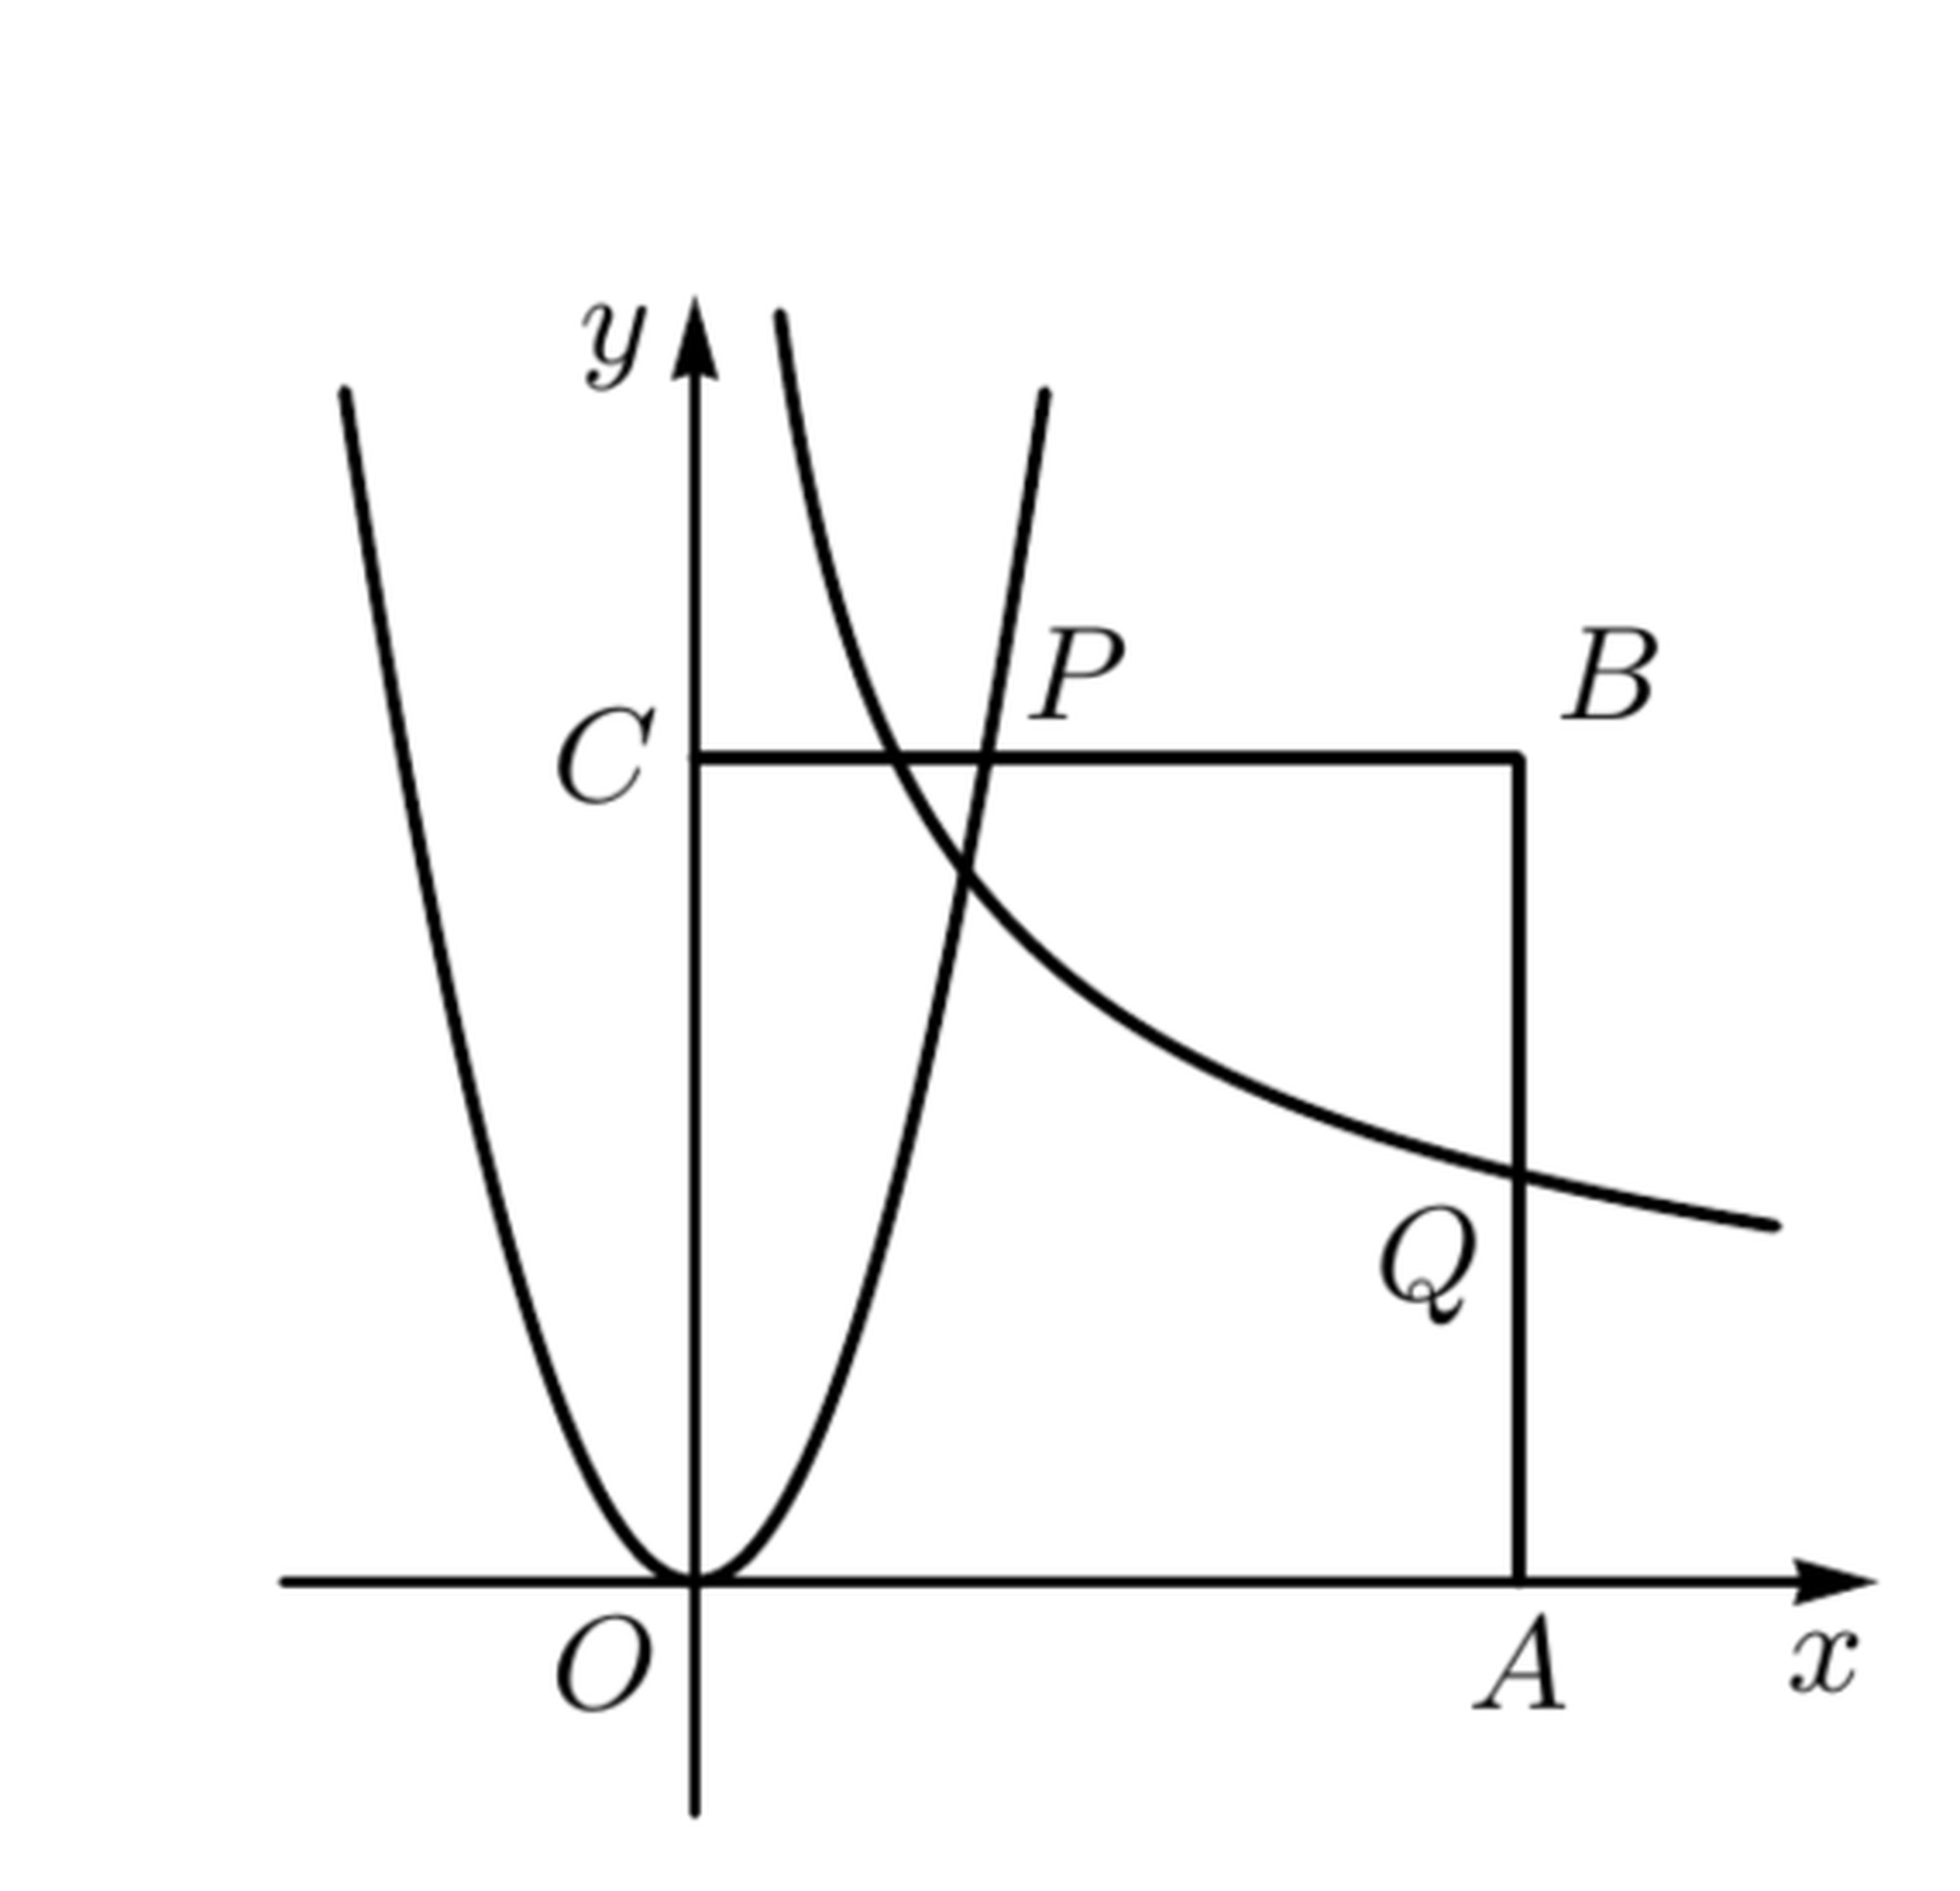
\includegraphics[width=0.40\textwidth]{figures/gao153_q11.png}
\end{center}

\ifanswer
\solbegin
\step{$\lvert AQ\rvert=\dfrac1{\sqrt a}$，$\lvert CP\rvert=\sqrt{\dfrac a5}$，}
\step{于是 $\lvert AQ\rvert+\lvert CP\rvert=\dfrac1{\sqrt a}+\sqrt{\dfrac a5}\geqslant2\sqrt{\dfrac1{\sqrt a}\cdot\sqrt{\dfrac a5}}=\dfrac2{\sqrt[4]{5}}$，}
\step{当且仅当 $\dfrac1{\sqrt a}=\sqrt{\dfrac a5}$，即 $a=\sqrt5$ 时取等号.}
\solend
\fi

% === Q12 === $B\subseteq A$ 带下划线照录、空集 \varnothing；解析 5 行
\item 若集合 $A=\{x\mid1\leqslant x\leqslant100,x\in\Z\}$，集合 $B\subseteq A$，且 $B\ne\varnothing$，记 $W(B)$ 为 $B$ 中元素的最大值与最小值之和，则对所有的 $B$，$W(B)$ 的平均值是\blankline[4.4em].

\ifanswer
\solbegin
\step{对每个非空子集 $B$，令 $B'=\{101-x\mid x\in B\}$，}
\step{则 $W(B')=(101-\min B)+(101-\max B)=202-W(B)$.}
\step{对 $B'$ 再作同样变换即得到 $B$，因此 $B$ 遍历所有非空子集时，}
\step{$B'$ 也恰好遍历所有非空子集.}
\step{设所求平均值为 $m$，则 $m=202-m$，解得 $m=101$.}
\solend
\fi

\end{enumerate}

\bigsec{二、选择题}

\begin{enumerate}
\setcounter{enumi}{12}

% === Q13 === "图像"（像，有亻）照录；解析 2 行，故选 A
\item 设 $a$、$b$ 为常数，若 $0<a<1$，$b>1$，则函数 $y=a^x-b$ 的图像必定不经过\mbox{（\quad）}

\keepwithprev
A. 第一象限\qquad\qquad B. 第二象限\qquad\qquad C. 第三象限\qquad\qquad D. 第四象限

\ifanswer
\solbegin
\step{当 $x>0$ 时，$a^x<1<b$，所以 $y=a^x-b<0$，图像必定不经过第一象限，}
\step{故选 $A$.}
\solend
\fi

% === Q14 === $m\in\Z$、中文弯引号、"图像"照录；解析 3 行，故选 A
\item 已知 $m\in\Z$，则“$m=0$”是“幂函数 $y=x^{m^2-2m-1}$ 的图像与 $x$ 轴及 $y$ 轴均无交点，且关于原点成中心对称”的\mbox{（\quad）}

\keepwithprev
A. 充分不必要条件\qquad\qquad B. 必要不充分条件

C. 充要条件\qquad\qquad D. 既不充分也不必要条件

\ifanswer
\solbegin
\step{图像满足所述条件 $\Leftrightarrow m^2-2m-1$ 为负奇数 $\Leftrightarrow m=0$ 或 $m=2$.}
\step{$m=0$ 能推出所述条件，但所述条件不能推出 $m=0$，因此是充分不必要条件，}
\step{故选 $A$.}
\solend
\fi

% === Q15 === 四选项一行；解析 5 行（跨 03→04 页），故选 D
\item 设 $a>b>1$，$x>1$，则下列不等式正确的是\mbox{（\quad）}

\keepwithprev
A. $a^x<b^x$\qquad B. $x^a<x^b$\qquad C. $\log_a x>\log_b x$\qquad D. $\log_x a>\log_x b$

\ifanswer
\solbegin
\step{$x>1$，幂函数与指数函数的单调性给出 $a^x>b^x$，$x^a>x^b$，A、B 错误.}
\step{$\log_a x=\dfrac{\lg x}{\lg a}<\dfrac{\lg x}{\lg b}=\log_b x$，C 错误.}
\step{对数函数 $y=\log_x t$ 的底数 $x>1$，在 $(0,+\infty)$ 上严格递增，}
\step{所以 $\log_x a>\log_x b$，D 正确.}
\step{故选 $D$.}
\solend
\fi

% === Q16 === $a\in\N$；解析 3 行，故选 C
\item 设 $a\in\N$，则满足不等式 $x^2-a^2x-a^2-1<0$ 的整数 $x$ 的个数不可能是\mbox{（\quad）}

\keepwithprev
A. 1\qquad\qquad B. 50\qquad\qquad C. 100\qquad\qquad D. 2026

\ifanswer
\solbegin
\step{$(x+1)(x-a^2-1)<0\Leftrightarrow-1<x<a^2+1$. 整数解为 $0,1,\cdots,a^2$，共 $a^2+1$ 个.}
\step{$1=0^2+1$，$50=7^2+1$，$2026=45^2+1$，而 $100-1=99$ 不是完全平方数，}
\step{故选 $C$.}
\solend
\fi

\end{enumerate}

\bigsec{三、解答题}

\begin{enumerate}
\setcounter{enumi}{16}

% === Q17 === 补集上划线 \overline{A}、\subseteq 照录；解析 5 行
\item 已知全集 $U=\R$，集合 $A=\{x\mid x^2-x-2\geqslant0\}$，$B=\{x\mid x>-1\}$，$C=\{x\mid a-5<x<a\}$.

(1) 求 $A\cap B$、$A\cup B$；

(2) 若 $\overline{A}\cup C=C$，求实数 $a$ 的取值范围.

\ifanswer
\solbegin
\step{(1) $x^2-x-2=(x+1)(x-2)\geqslant0\Leftrightarrow x\leqslant-1$ 或 $x\geqslant2$，}
\step{所以 $A=(-\infty,-1]\cup[2,+\infty)$，$B=(-1,+\infty)$，}
\step{因此 $A\cap B=[2,+\infty)$，$A\cup B=\R$.}
\step{(2) $\overline{A}=(-1,2)$，于是 $\overline{A}\cup C=C\Leftrightarrow\overline{A}\subseteq C\Leftrightarrow(-1,2)\subseteq(a-5,a)$，}
\step{两区间均为开区间，端点可重合，故 $\begin{cases}a-5\leqslant-1\\a\geqslant2\end{cases}\Leftrightarrow2\leqslant a\leqslant4$.}
\solend
\fi

% === Q18 === 解析 4 行
\item 已知 $a$、$b$、$c$ 都是正数，

(1) 若 $a+b=1$，求证：$\dfrac1a+\dfrac1b\geqslant4$，并指出等号成立的条件；

(2) 若 $a+b+c=1$，求证：三个数 $\dfrac1a$、$\dfrac1b$、$\dfrac1c$ 中至少有一个不小于 3.

\ifanswer
\solbegin
\step{(1) 由 $(a-b)^2\geqslant0$，得 $4ab\leqslant(a+b)^2=1$，所以 $\dfrac1a+\dfrac1b=\dfrac{a+b}{ab}=\dfrac1{ab}\geqslant4$，}
\step{等号成立当且仅当 $a=b$，结合 $a+b=1$，得 $a=b=\dfrac12$.}
\step{(2) 假设三个数 $\dfrac1a$、$\dfrac1b$、$\dfrac1c$ 都小于 3，则 $a>\dfrac13,b>\dfrac13,c>\dfrac13\Rightarrow a+b+c>1$，}
\step{与 $a+b+c=1$ 矛盾，因此三个数中至少有一个不小于 3.}
\solend
\fi

% === Q19 === 题目配图（三版都出）；\needvspace 守卫放 \item 之前；解析 19 行
\needvspace{8cm}
\item 某新建居民小区有一直角三角形绿地，两直角边长分别为 30m 和 40m，打算在其中划出一片区域改造成活动场地，如图所示.

(1) 若划出的区域为正方形，且有两边落在绿地边界上，求此正方形边长；

(2) 若划出的区域为圆形，求圆形区域面积的最大值；

(3) 若划出的区域为矩形（其中至少有一边在边界上），求此矩形面积的最大值.

\begin{center}
% 直角三角形 ABC 绿地示意图取 05 页右上，去粉色水印、去色、4× LANCZOS 放大；三版都出
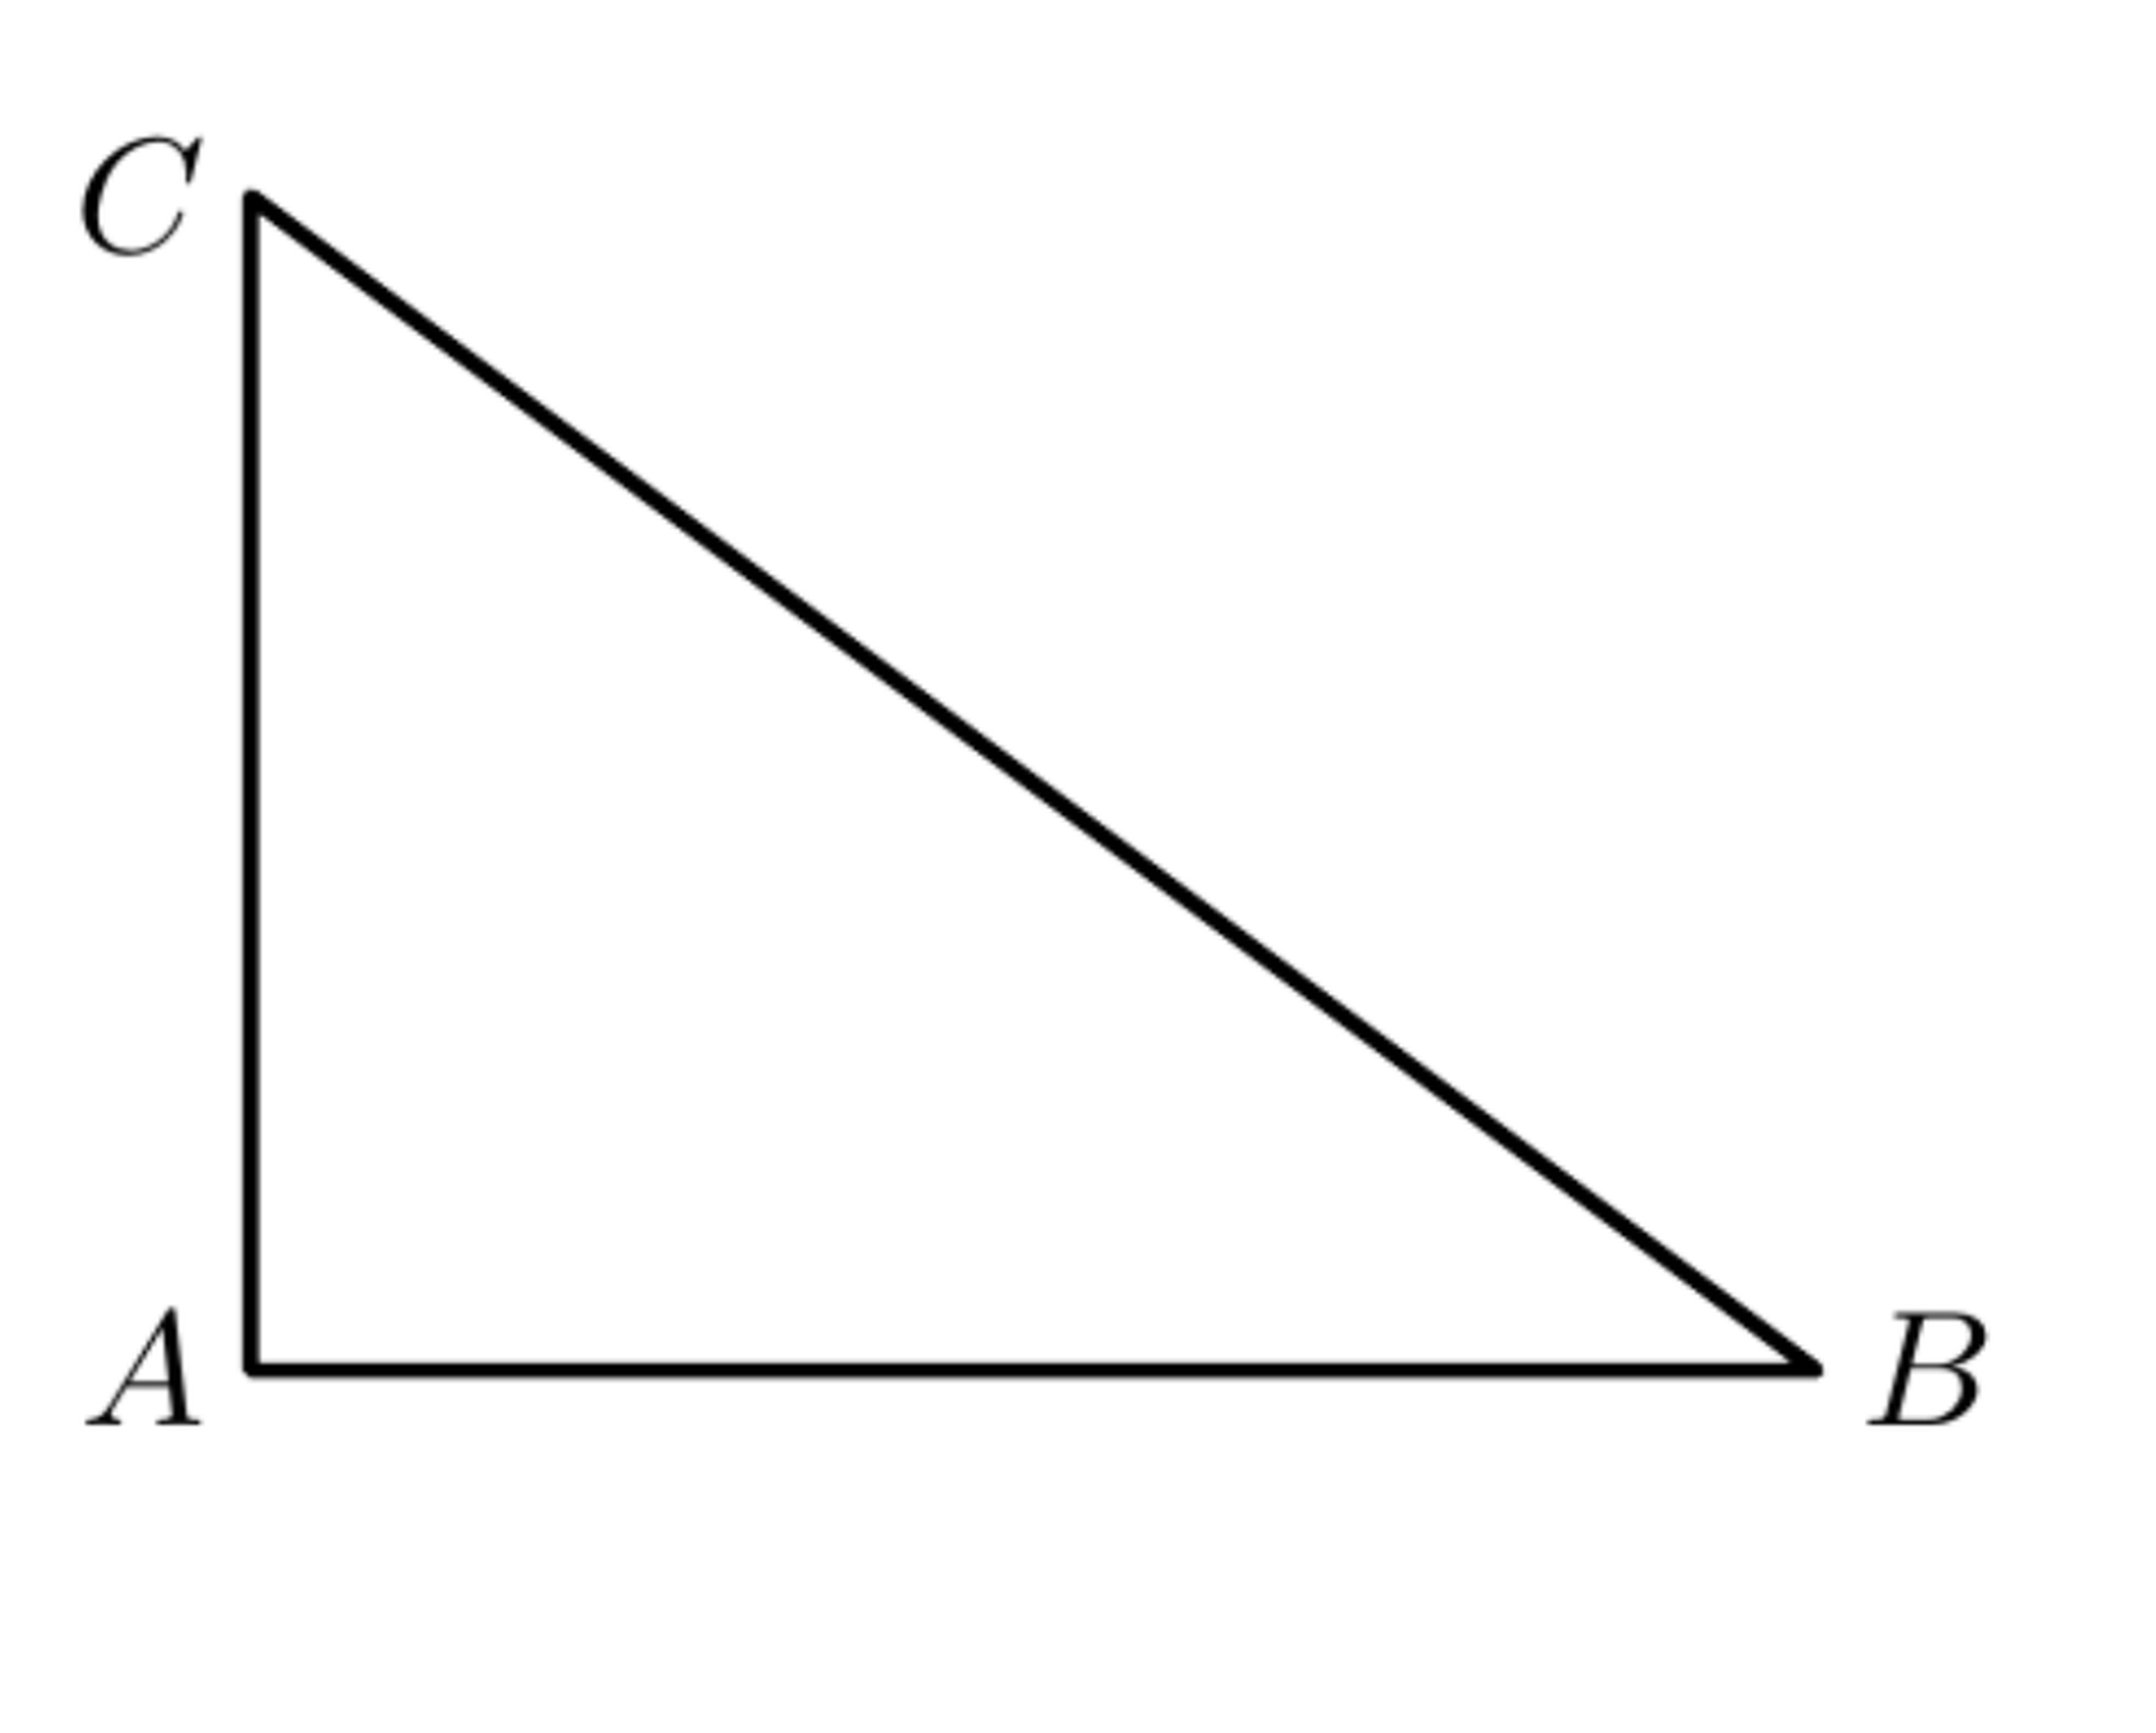
\includegraphics[width=0.34\textwidth]{figures/gao153_q19.png}
\end{center}

\ifanswer
\solbegin
\step{(1) 取 $A(0,0)$、$B(40,0)$、$C(0,30)$，则斜边 $BC$ 所在直线为 $3x+4y=120$.}
\step{正方形落在边界上的两边必分别在两条直角边上.}
\step{设其边长为 $a$m，则对角顶点为 $(a,a)$.}
\step{按题意划出的正方形应尽量大，即对角顶点落在斜边 $BC$ 上，}
\step{因此 $3a+4a=120\Rightarrow a=\dfrac{120}{7}$；}
\step{(2) 斜边长 $BC=\sqrt{30^2+40^2}=50$m，三角形面积为 $600\text{m}^2$.}
\step{设圆的半径为 $r$，圆心到 $AB$、$AC$、$BC$ 的距离分别为 $d_1,d_2,d_3$，}
\step{则三者均不小于 $r$. 连接圆心与三个顶点，}
\step{得 $600=\dfrac12(40d_1+30d_2+50d_3)\geqslant\dfrac12(40+30+50)r=60r$，所以 $r\leqslant10$.}
\step{取三角形的内切圆时等号成立，圆形区域面积的最大值为 $100\pi\text{m}^2$.}
\step{(3) 任取矩形落在绿地边界上的一边，以其所在直线为横轴.}
\step{设相应三角形底边长为 $L$、高为 $H$，则 $LH=1200$.}
\step{取三角形顶点坐标为 $(0,0)$、$(L,0)$、$(p,H)$.}
\step{在高度 $t$ 处，两腰上的点的横坐标分别为 $\dfrac{pt}{H}$、$L+\dfrac{(p-L)t}{H}$，}
\step{因此，高为 $t$ 的矩形，其底边长不超过 $L\left(1-\dfrac tH\right)$，}
\step{面积满足 $S\leqslant Lt\left(1-\dfrac tH\right)=\dfrac LH\left[\dfrac{H^2}{4}-\left(t-\dfrac H2\right)^2\right]\leqslant\dfrac{LH}{4}=300$，}
\step{在原坐标系中，取矩形顶点为 $(0,0)$、$(20,0)$、$(20,15)$、$(0,15)$，}
\step{其中 $3\times20+4\times15=120$，矩形完全位于绿地内，面积为 $300\text{m}^2$，}
\step{达到最大值.}
\solend
\fi

% === Q20 === $g(x)$ 定义照录；解析 14 行
\item 已知 $a>0$ 且 $a\ne1$，设 $f(x)=\log_a(x^2-a^2)$，$g(x)=2\log_a(x-ak)$.

(1) 求函数 $y=f(x)$ 的定义域；

(2) 若 $k=2$，求不等式 $f(x)>g(x)$ 的解集；

(3) 若“存在实数 $x$，使得 $f(x)=g(x)$”为真命题，求实数 $k$ 的取值范围.

\ifanswer
\solbegin
\step{(1) $x^2-a^2>0\Leftrightarrow x<-a$ 或 $x>a$，定义域为 $(-\infty,-a)\cup(a,+\infty)$.}
\step{(2) 两函数均有意义时，$x>2a$，且 $g(x)=\log_a(x-2a)^2$.}
\step{当 $a>1$ 时，$f(x)>g(x)\Leftrightarrow x^2-a^2>(x-2a)^2\Leftrightarrow x>\dfrac{5a}{4}$，}
\step{结合 $x>2a$，解集为 $(2a,+\infty)$.}
\step{当 $0<a<1$ 时，$f(x)>g(x)\Leftrightarrow x^2-a^2<(x-2a)^2\Leftrightarrow x<\dfrac{5a}{4}$，}
\step{与 $x>2a$ 矛盾，解集为 $\varnothing$.}
\step{(3) 在 $x^2-a^2>0$ 且 $x-ak>0$ 的条件下，}
\step{$f(x)=g(x)\Leftrightarrow x^2-a^2=(x-ak)^2\Leftrightarrow2akx=a^2(1+k^2)$，}
\step{当 $k=0$ 时，上式不成立；}
\step{当 $k\ne0$ 时，$x=\dfrac{a(1+k^2)}{2k}$，}
\step{于是 $x-ak=\dfrac{a(1-k^2)}{2k}>0\Leftrightarrow k<-1$ 或 $0<k<1$，}
\step{对上述 $k$，所取的 $x$ 同时满足 $x^2-a^2=(x-ak)^2>0$，}
\step{两函数均有意义且函数值相等.}
\step{因此，$k$ 的取值范围为 $(-\infty,-1)\cup(0,1)$.}
\solend
\fi

% === Q21 === 中文弯引号、复杂式照录；解析 23 行（跨 08→09 页）
\item 若实数 $x$、$y$、$m$ 满足 $\lvert x-m\rvert<\lvert y-m\rvert$，则称 $x$ 比 $y$ 接近 $m$.

(1) 若 $2x$ 比 $x-2$ 更接近 1，求实数 $x$ 的取值范围；

(2) 若 $x$ 比 $y$ 接近 $m$，证明：“$x>y$” 的充要条件是 “$x+y<2m$”；

(3) 已知 $x>0$，$y>0$ 且 $x\ne y$. 设 $p=\dfrac{x^2+y^2}{xy}$，若对于任意的 $x$、$y$，命题 “$p$ 比 $p^2-3p+4$ 接近 $m$” 恒成立，求实数 $m$ 的取值范围.

\ifanswer
\solbegin
\step{(1) $\lvert2x-1\rvert<\lvert x-3\rvert\Leftrightarrow(2x-1)^2<(x-3)^2\Leftrightarrow(x+2)(3x-4)<0$，}
\step{解得 $-2<x<\dfrac43$，实数 $x$ 的取值范围为 $\left(-2,\dfrac43\right)$.}
\step{(2) 因为 $x$ 比 $y$ 接近 $m$，所以 $\lvert x-m\rvert<\lvert y-m\rvert$，则 $\lvert x-m\rvert^2<\lvert y-m\rvert^2$，}
\step{即 $(x-m)^2<(y-m)^2$，即 $(x-m)^2-(y-m)^2<0$，}
\step{即得 $(x-y)(x+y-2m)<0$，}
\step{则由 $x+y<2m$，得 $x+y-2m<0$，}
\step{故 $x-y>0$，即 $x>y$，充分性成立；}
\step{当 $x>y$ 时，$x-y>0$，结合 $(x-y)(x+y-2m)<0$，得 $x+y-2m<0$，}
\step{即 $x+y<2m$，必要性成立；}
\step{故“$x>y$” 的充要条件是 “$x+y<2m$”；}
\step{(3) $x>0$，$y>0$ 且 $x\ne y$. 则 $p=\dfrac{x^2+y^2}{xy}=\dfrac xy+\dfrac yx>2\sqrt{\dfrac xy\cdot\dfrac yx}=2$，}
\step{由于对于任意的 $x$、$y$，命题 “$p$ 比 $p^2-3p+4$ 接近 $m$” 恒成立，}
\step{故 $\lvert p-m\rvert<\lvert(p^2-3p+4)-m\rvert$ 对 $\forall p>2$ 恒成立，}
\step{即得 $(p-m)^2<(p^2-3p+4-m)^2$，}
\step{即 $(p^2-3p+4-m)^2-(p-m)^2>0$，}
\step{得 $(p^2-4p+4)(p^2-2p+4-2m)>0$，}
\step{即 $(p-2)^2(p^2-2p+4-2m)>0$，由于 $p>2$，故 $(p-2)^2>0$，}
\step{故 $p^2-2p+4-2m>0$ 对 $\forall p>2$ 恒成立，}
\step{即 $2m<p^2-2p+4$ 对 $\forall p>2$ 恒成立，}
\step{由于 $p^2-2p+4=(p-1)^2+3$，此时 $p^2-2p+4$ 在 $(2,+\infty)$ 上严格增，}
\step{故 $(p-1)^2+3>(2-1)^2+3=4$，故 $2m\leqslant4$，解得 $m\leqslant2$，}
\step{即实数 $m$ 的取值范围是 $(-\infty,2]$.}
\solend
\fi

\end{enumerate}

\end{document}
"
% 紧凑版：xelatex "\def\iscompact{1}% 高一153_闵行中学文绮中学_期中.tex
%   —— 高一上数学"2026-2027 年闵行中学文绮中学高一上期中"（试卷版/答案版/紧凑版）
% 试卷版：xelatex 高一153_闵行中学文绮中学_期中.tex
% 答案版：xelatex "\def\isanswer{1}\input{高一153_闵行中学文绮中学_期中.tex}"
% 紧凑版：xelatex "\def\iscompact{1}\input{高一153_闵行中学文绮中学_期中.tex}"
%
% ① 原始材料：微信公众号"魔都数学加油站"文章，连载"27学年高一153"，原文标题
% "27学年高一153——2026-2027年上海市闵行中学文绮中学高一上期中"；
% 原文链接：https://mp.weixin.qq.com/s/rEtS-92cDR6JKgY2b5DRfg 。
% 正文为 9 张 PNG 页（01/02/06/07/08/09 为 2560×3620，03/04/05 为 4762×6735，
% 同一篇各页分辨率混排，逐页按各自分辨率裁图核对，别按预览比例换算裁框）。
% 体例：讲评版——填空 3—12（10 题）、选择 13—16（4 题）、解答 17—21（5 题），
% 共 19 题，自第 3 题起编；**全 19 题均印【解析】**（逐题核实，见 ② ②）。
% 题目、答案、解析均据原图转录；卷面粉红色水印"魔都数学加油站"及公众号页脚未录入。
% 全卷插图清单（逐页通读 9 页确认）：2 幅，均为题目配图、三版都出——
%   · Q11 正方形 OABC 曲线图（02 页右下：$y=5x^2$ 与 $y=x^{-\frac12}$ 两条曲线、
%     坐标轴、O/A/B/C/P/Q、正方形），裁 figures/gao153_q11.png；
%   · Q19 直角三角形 ABC 绿地示意图（05 页右上，直角在 A），
%     裁 figures/gao153_q19.png；
%   两图均去粉色水印、去色、4× LANCZOS 放大；Q11 图左上角题干残字"函"已裁白。
%   其余各页逐页确认无其它题目配图、无解析内配图、无表格；09 页下半仅水印、无正文。
%
% 卷首标题：原卷印作"2026-2027 年闵行中学文绮中学高一上期中"，年份区间按全稿惯例排 en dash；
% 原卷卷面未印副标题，本稿按同期中卷知识模块口径补出"集合与常用逻辑用语、不等式、函数"。
%
% ② 与原卷的排版差异：
%   ① 原文从第 3 题起，本稿保留原题号；共 19 题三节，解答题 5 题到 21；
%   ② 全 19 题均印【解析】、用 \solbegin…\solend，无只印【答案】或答案印括号内的题；
%      四道选择题答案在解析末句"故选 A／A／D／C"（Q13—Q16，逐个放大复核）、
%      括号 \mbox{（\quad）} 留空、不另提 \ans{}；答案版【答案】/【解析】标记数
%      = 19 = 全卷题数；
%   ③ 原卷卷面未印副标题，本稿按知识模块口径补出；
%   ④ 原卷填空横线按全稿惯例排 \blankline[4.4em]；选择题括号排 \mbox{（\quad）}、
%      四道选择题的选项段前按惯例各加 \keepwithprev；解答题不留作答区、不加
%      \anspace（原卷为讲评版，109—113 起全稿不用 \anspace）；
%   ⑤ 数集：Q3"$x\in R$"、Q5"解集为 R"、Q10"$x\in N$"、Q12"$x\in Z$"与
%      "$m\in Z$"、Q14"$m\in Z$"、Q16"$a\in N$"、Q17"全集 $U=R$"、
%      Q19 无、Q21 无——原卷印斜体或正体粗体 R/N/Z，按全稿惯例归一
%      \R／\N／\Z；绝对值排 \lvert…\rvert（Q5、Q11、Q21），集合描述竖线排 \mid
%      （Q3、Q10、Q17、Q20），不等号按全稿惯例排 \leqslant／\geqslant；
%      补集照原卷上划线排 \overline{A}（Q17 题干 (2)＋解析 (2)）；
%      空集 \varnothing（Q12 题干、Q20 解析 (2)）；子集 3 处均印带下划线 ⊆、
%      照录 \subseteq（Q10 $A\subseteq U$、Q12 $B\subseteq A$、Q17 $(-1,2)\subseteq(a-5,a)$），
%      本卷无单线 \subset 用例；
%   ⑥ 判别式：逐页通读 9 页，本卷无一元二次判别式 Δ/△ 算式，故无 Δ/△ 混用可照录；
%      Q11 图里有几何正方形 OABC（非三角形符号），无 △ABC 用例；
%   ⑦ 中文弯引号照录：Q14"$m=0$"与"幂函数…关于原点成中心对称"、
%      Q20"存在实数 $x$，使得 $f(x)=g(x)$"、Q21"$x>y$"与"$x+y<2m$"、
%      "$p$ 比 $p^2-3p+4$ 接近 $m$"（引号外留空格按原卷）；
%      注释里一律 ASCII 引号；数学式内 CJK 用 \text{}；
%   ⑧ "图像／图象"逐处放大核：全卷 3 处均印"图像"（像，有亻）——
%      Q13 题干与解析、Q14 题干与解析；Q19 题干写"如图所示"（非"图像"），
%      逐处照录未统一；子题标号 (1)(2)(3) 半角括号照录；圈数字本卷无用例；
%   ⑨ 半角逗号在数学组之间是全稿惯例、非笔误，逐处照录（Q3 $x\in R$、
%      Q10 $a_1,a_2$、Q19 $A(0,0)$、$d_1,d_2,d_3$、Q21 $a>\frac13,b>\frac13$ 等）；
%      行末西文句点 ASCII `.`；行中全角逗号／顿号照录（Q19"30m 和 40m"、
%      Q21"实数 $x$、$y$、$m$"）；
%   ⑩ 复杂式照录别简化：Q3 $y=x^{-2}$、Q11 $y=x^{-\frac12}$ 与
%      $\frac{2}{\sqrt[4]{5}}$、Q8 $\frac{2b}{a+1-b}$、Q9 cases 块、
%      Q10 $525=5\times105$、Q16 $a^2+1$、Q19 $S\leqslant Lt(1-\frac tH)$
%      与 $L+\frac{(p-L)t}{H}$、Q20 $2akx=a^2(1+k^2)$ 与 $\frac{a(1+k^2)}{2k}$、
%      Q21 $(p^2-4p+4)(p^2-2p+4-2m)>0$；
%      \left…\right 不得拆到不同 $…$ 组（Q17 $\left\{x\mid\cdots\right\}$、
%      Q19 $\left[\frac{H^2}{4}-\left(t-\frac H2\right)^2\right]$、
%      Q21 $\left(-2,\frac43\right)$ 等）；cases 块一律 \begin{cases}…\end{cases}；
%   ⑪ 一条 \step = 原卷解析的一个印刷行，cases 块整体算一个印刷行；别并折行、
%      别拆行。Q10 六行、Q19 十九行、Q20 十四行、Q21 二十二行均按印刷行逐条断，
%      不丢行；
%   ⑫ 配图：Q11／Q19 题目配图（三版都出）放 \item 内题干之后 \begin{center}，
%      各用 \needvspace{8cm} 守卫把整块推走，**守卫放在 \item 之前**
%      （见 高一145 Q14/Q20 成例与切页审计 B 类坑）；
%   ⑬ 原卷解析内无红色"法一／法二"之类小标题，故本卷无 \stepm；红色水印
%      "魔都数学加油站"不录入；
%   ⑭ 跨页续印按题合并：见 ⑥；
%
% ③ 行数复核：一条 \step = 原卷解析的一个印刷行，cases 块作一个印刷行计。
%   逐题数（主会话逐页核对定稿）：Q3：1；Q4：2；Q5：2；Q6：2；Q7：1；
%   Q8：1；Q9：2；Q10：6；Q11：3；Q12：5；Q13：2；Q14：3；Q15：5；
%   Q16：3；Q17：5；Q18：4；Q19：19；Q20：14；Q21：22。
%   合计 102 条 \step（本卷无 \stepm），与原卷逐题印刷行相等。全卷 19 题
%   均设 \solbegin…\solend，答案版【答案】/【解析】标记数 = 19 = 全卷题数。
%
% ④ 判别式／子集符号结论（逐处放大原图照录、不得统一，主会话像素级复核）：
%   判别式：逐页通读 9 页，本卷无一元二次判别式算式（Q7 用韦达定理、
%      Q16 用因式分解、Q20 用对数方程，均不写 Δ/△），故无 Δ/△ 混用可照录
%      （"高 \Delta／扁 \triangle"口径备查，参照 高一142／151／152 头注）；
%      本卷无几何三角形符号用例。
%   子集：Q10 题干"$A\subseteq U$"、Q12 题干"$B\subseteq A$"、Q17 解析 (2)
%      "$(-1,2)\subseteq(a-5,a)$"共 3 处，逐处放大确认均印带下划线 ⊆、
%      照录 \subseteq；本卷未见单线 ⊂（\subset）之对应处。
%      补集上划线 \overline{A}（Q17）、空集 \varnothing（Q12 题干、Q20 解析 (2)）；
%      数集 \R／\N／\Z 归一见 ② ⑤。
%
% ⑤ 存疑照录（放大原图确认，照录未改、正文对应处另有 % 注）：
%   1. Q3 集合 $B=\{(x,y)\mid y=x^{-2},x\in\R\}$ 原卷题干径写 $x\in\R$
%      （$x=0$ 处无意义），解析自行注明 $x\ne0$，照录未改。
%   2. Q10 解析"$U$ 中共有 $525=5\times105$ 个连续整数"与尾行
%      "取 $U$ 中除以 5 余 1 或 2 的全部元素及元素 5"逐字照录（放大 02 页
%      /tmp/gao153/z/zoom/q10_pick.png 确认是"元素 5"，非"元素 9"）。
%   3. Q11 第二个函数原卷印 $y=x^{-\frac12}$（负二分之一次幂，非 $x^2$），
%      放大 02 页 /tmp/gao153/z/zoom/q11_exp.png 确认，照录未改；
%      $|AQ|=\frac1{\sqrt a}$ 与之自洽。
%   4. Q19 (3) 解析"在高度 $t$ 处，两腰上的点的横坐标分别为 $\frac{pt}{H}$、
%      $L+\frac{(p-L)t}{H}$"，放大 06 页确认，照录未简化。
%   5. Q20 (2) 解析"$g(x)=\log_a(x-2a)^2$"（真数整体平方），
%      与 $g(x)=2\log_a(x-ak)$ 在 $k=2$ 时一致，照录未改。
%   6. Q21 (3) 解析"得 $(p^2-4p+4)(p^2-2p+4-2m)>0$"与
%      "故 $(p-1)^2+3>(2-1)^2+3=4$，故 $2m\leqslant4$"照录未改
%      （放大 09 页 /tmp/gao153/z/zoom/q21_factor.png 确认）。
%   7. "图像／图象"全卷 3 处均印"图像"（像，有亻）逐处照录；
%      本卷无判别式 Δ/△ 用例（见 ④）。
%   全卷除此 7 类外未发现其它笔误／自相矛盾处；19 题均印【解析】、
%   无只印【答案】或答案印括号内的题（见 ② ②）。
%
% ⑥ 跨页续印按题合并说明（逐页核实定稿）：Q3—Q5 题干＋解析在 01 页；
%   Q6—Q8 题干＋解析在 01 页下半（Q8 解析续 02 页顶）；Q9 题干＋解析、
%   Q10 题干＋解析首 2 行在 02 页上半，Q10 解析余 4 行在 02 页下半；
%   Q11 题干＋配图＋解析、Q12 题干＋解析 5 行在 02 页下半—03 页上半；
%   "二、选择题"标题在 03 页中部；Q13 题干＋选项＋解析在 03 页下半；
%   Q14 题干＋选项＋解析、Q15 题干＋选项＋解析首行在 03 页下半—04 页顶；
%   Q15 解析余 4 行、Q16 题干＋选项＋解析在 04 页上半；"三、解答题"
%   标题在 04 页下半；Q17 题干＋两问＋解析 5 行在 04 页下半—05 页顶；
%   Q18 题干＋两问＋解析 4 行、Q19 题干（含配图）＋三问在 05 页；
%   Q19 解析 (1)(2) 9 行在 05 页下半，解析 (3) 前 5 行在 06 页上半、
%   余 4 行在 06 页下半；Q20 题干＋三问在 06 页下半，解析 (1)(2)(3)
%   前 6 行在 07 页上半、(3) 余 8 行在 07 页下半；Q21 题干＋三问在
%   07 页末，解析 (1)(2) 10 行在 08 页上半—下半，解析 (3) 前 4 行在
%   08 页下半、余 9 行续 09 页上半，末行"即实数 $m$ 的取值范围是
%   $(-\infty,2]$"为全卷收尾（09 页下半仅水印、无正文）。
%   本稿按题连排，不丢行、不并折行；全卷末题为第 21 题，无附加题节。
%
\documentclass[a4paper,11pt]{article}
\usepackage{common}

\begin{document}

\examtitlest[3]{2026--2027 年闵行中学文绮中学高一上期中}{集合与常用逻辑用语、不等式、函数}

\bigsec{一、填空题}

\begin{enumerate}
\setcounter{enumi}{2}

% === Q3 === 集合描述竖线 \mid；$y=x^{-2}$ 照录；解析 1 行
\item 已知 $A=\{(x,y)\mid y=x^3,x\in\R\}$，$B=\{(x,y)\mid y=x^{-2},x\in\R\}$，则 $A\cap B=$\blankline[4.4em].

\ifanswer
\solbegin
\step{$x^3=x^{-2}\ (x\ne0)\Leftrightarrow x^5=1\Leftrightarrow x=1$，此时 $y=1$，所以 $A\cap B=\{(1,1)\}$.}
\solend
\fi

% === Q4 === 解析 2 行
\item 若关于 $x$ 的不等式 $\dfrac{x-a}{x+1}>0$ 的解集为 $(-\infty,-1)\cup(4,+\infty)$，则实数 $a=$\blankline[4.4em].

\ifanswer
\solbegin
\step{关于 $x$ 的不等式 $\dfrac{x-a}{x+1}>0$ 即 $(x+1)(x-a)>0$.}
\step{再由它的解集为 $(-\infty,-1)\cup(4,+\infty)$，得 $-1$ 和 4 是 $(x+1)(x-a)=0$ 的两个实数根，故 $a=4$.}
\solend
\fi

% === Q5 === 绝对值 \lvert…\rvert；解析 2 行
\item 若关于 $x$ 的不等式 $\lvert x+1\rvert+\lvert x-2\rvert>m$ 的解集为 $\R$，则实数 $m$ 的取值范围是\blankline[4.4em].

\ifanswer
\solbegin
\step{$\lvert x+1\rvert+\lvert x-2\rvert\geqslant\lvert(x+1)-(x-2)\rvert=3$，当且仅当 $-1\leqslant x\leqslant2$ 时取等号，}
\step{因此 $m<3$.}
\solend
\fi

% === Q6 === 解析 2 行
\item 已知指数函数 $y=a^x$（$a>1$）在区间 $[-1,1]$ 上的最大值比最小值大 $\dfrac32$，则实数 $a=$\blankline[4.4em].

\ifanswer
\solbegin
\step{$a>1$，指数函数在 $[-1,1]$ 上严格增，故 $a-\dfrac1a=\dfrac32\Leftrightarrow(a-2)(2a+1)=0$.}
\step{结合 $a>1$，得 $a=2$.}
\solend
\fi

% === Q7 === 韦达定理；解析 1 行
\item 已知关于 $x$ 的一元二次方程 $x^2+px+2p=0$ 的两个实数根分别为 $x_1$、$x_2$，且 $(x_1+1)(x_2+1)=0$，则 $p=$\blankline[4.4em].

\ifanswer
\solbegin
\step{$0=(x_1+1)(x_2+1)=x_1x_2+x_1+x_2+1=2p-p+1=p+1\Rightarrow p=-1$.}
\solend
\fi

% === Q8 === 换底公式；解析 1 行
\item 已知 $10^a=3$，$\lg5=b$，则 $\log_6 25=$\blankline[4.4em]（用关于 $a,b$ 的关系式表示）.

\ifanswer
\solbegin
\step{$\lg3=a$，$\lg2=1-b$，所以 $\log_6 25=\dfrac{\lg25}{\lg6}=\dfrac{2b}{a+1-b}$.}
\solend
\fi

% === Q9 === cases 块整体算一个印刷行；解析 2 行
\item 已知 $A=[2,5]$，若对任意 $x\in A$，总有 $\dfrac{k}{x}\in A$，则正数 $k=$\blankline[4.4em].

\ifanswer
\solbegin
\step{$k>0$，当 $x\in[2,5]$ 时，$\dfrac{k}{x}$ 的取值范围为 $\left[\dfrac k5,\dfrac k2\right]$，}
\step{因此 $\begin{cases}\dfrac k5\geqslant2\\\dfrac k2\leqslant5\end{cases}\Leftrightarrow10\leqslant k\leqslant10\Leftrightarrow k=10$.}
\solend
\fi

% === Q10 === $A\subseteq U$ 带下划线照录；解析 6 行
\item 已知集合 $U=\{x\mid4\leqslant x\leqslant528,x\in\N\}$，$A=\{a_1,a_2,a_3,\cdots,a_n\}$，且 $A\subseteq U$. 如果集合 $A$ 中的任意两个不同元素之和都不能被 5 整除，则正整数 $n$ 的最大值为\blankline[4.4em].

\ifanswer
\solbegin
\step{$U$ 中共有 $525=5\times105$ 个连续整数，按除以 5 的余数分成五类，}
\step{每类均有 105 个元素.}
\step{余数为 1,4 的两类不能同时选取，余数为 2,3 的两类也不能同时选取，}
\step{余数为 0 的一类最多选 1 个，因此 $n\leqslant105+105+1=211$.}
\step{取 $U$ 中除以 5 余 1 或 2 的全部元素及元素 5，}% 放大 02 页确认是「元素 5」（非 9），照录未改（见 ⑤ 2）
\step{任意两个不同元素之和均不能被 5 整除，此时 $n=211$，最大值为 211.}
\solend
\fi

% === Q11 === 题目配图（三版都出）；\needvspace 守卫放 \item 之前；$y=x^{-\frac12}$ 照录；解析 3 行
\needvspace{8cm}
\item 如图，已知正方形 $OABC$，其中 $OA=a$（$a>1$），函数 $y=5x^2$ 交 $BC$ 于点 $P$，函数 $y=x^{-\frac12}$ 交 $AB$ 于点 $Q$，当 $\lvert AQ\rvert+\lvert CP\rvert$ 最小时，$a$ 的值为\blankline[4.4em].

\begin{center}
% 正方形 OABC 与两条曲线图取 02 页右下，去粉色水印、去色、4× LANCZOS 放大；三版都出
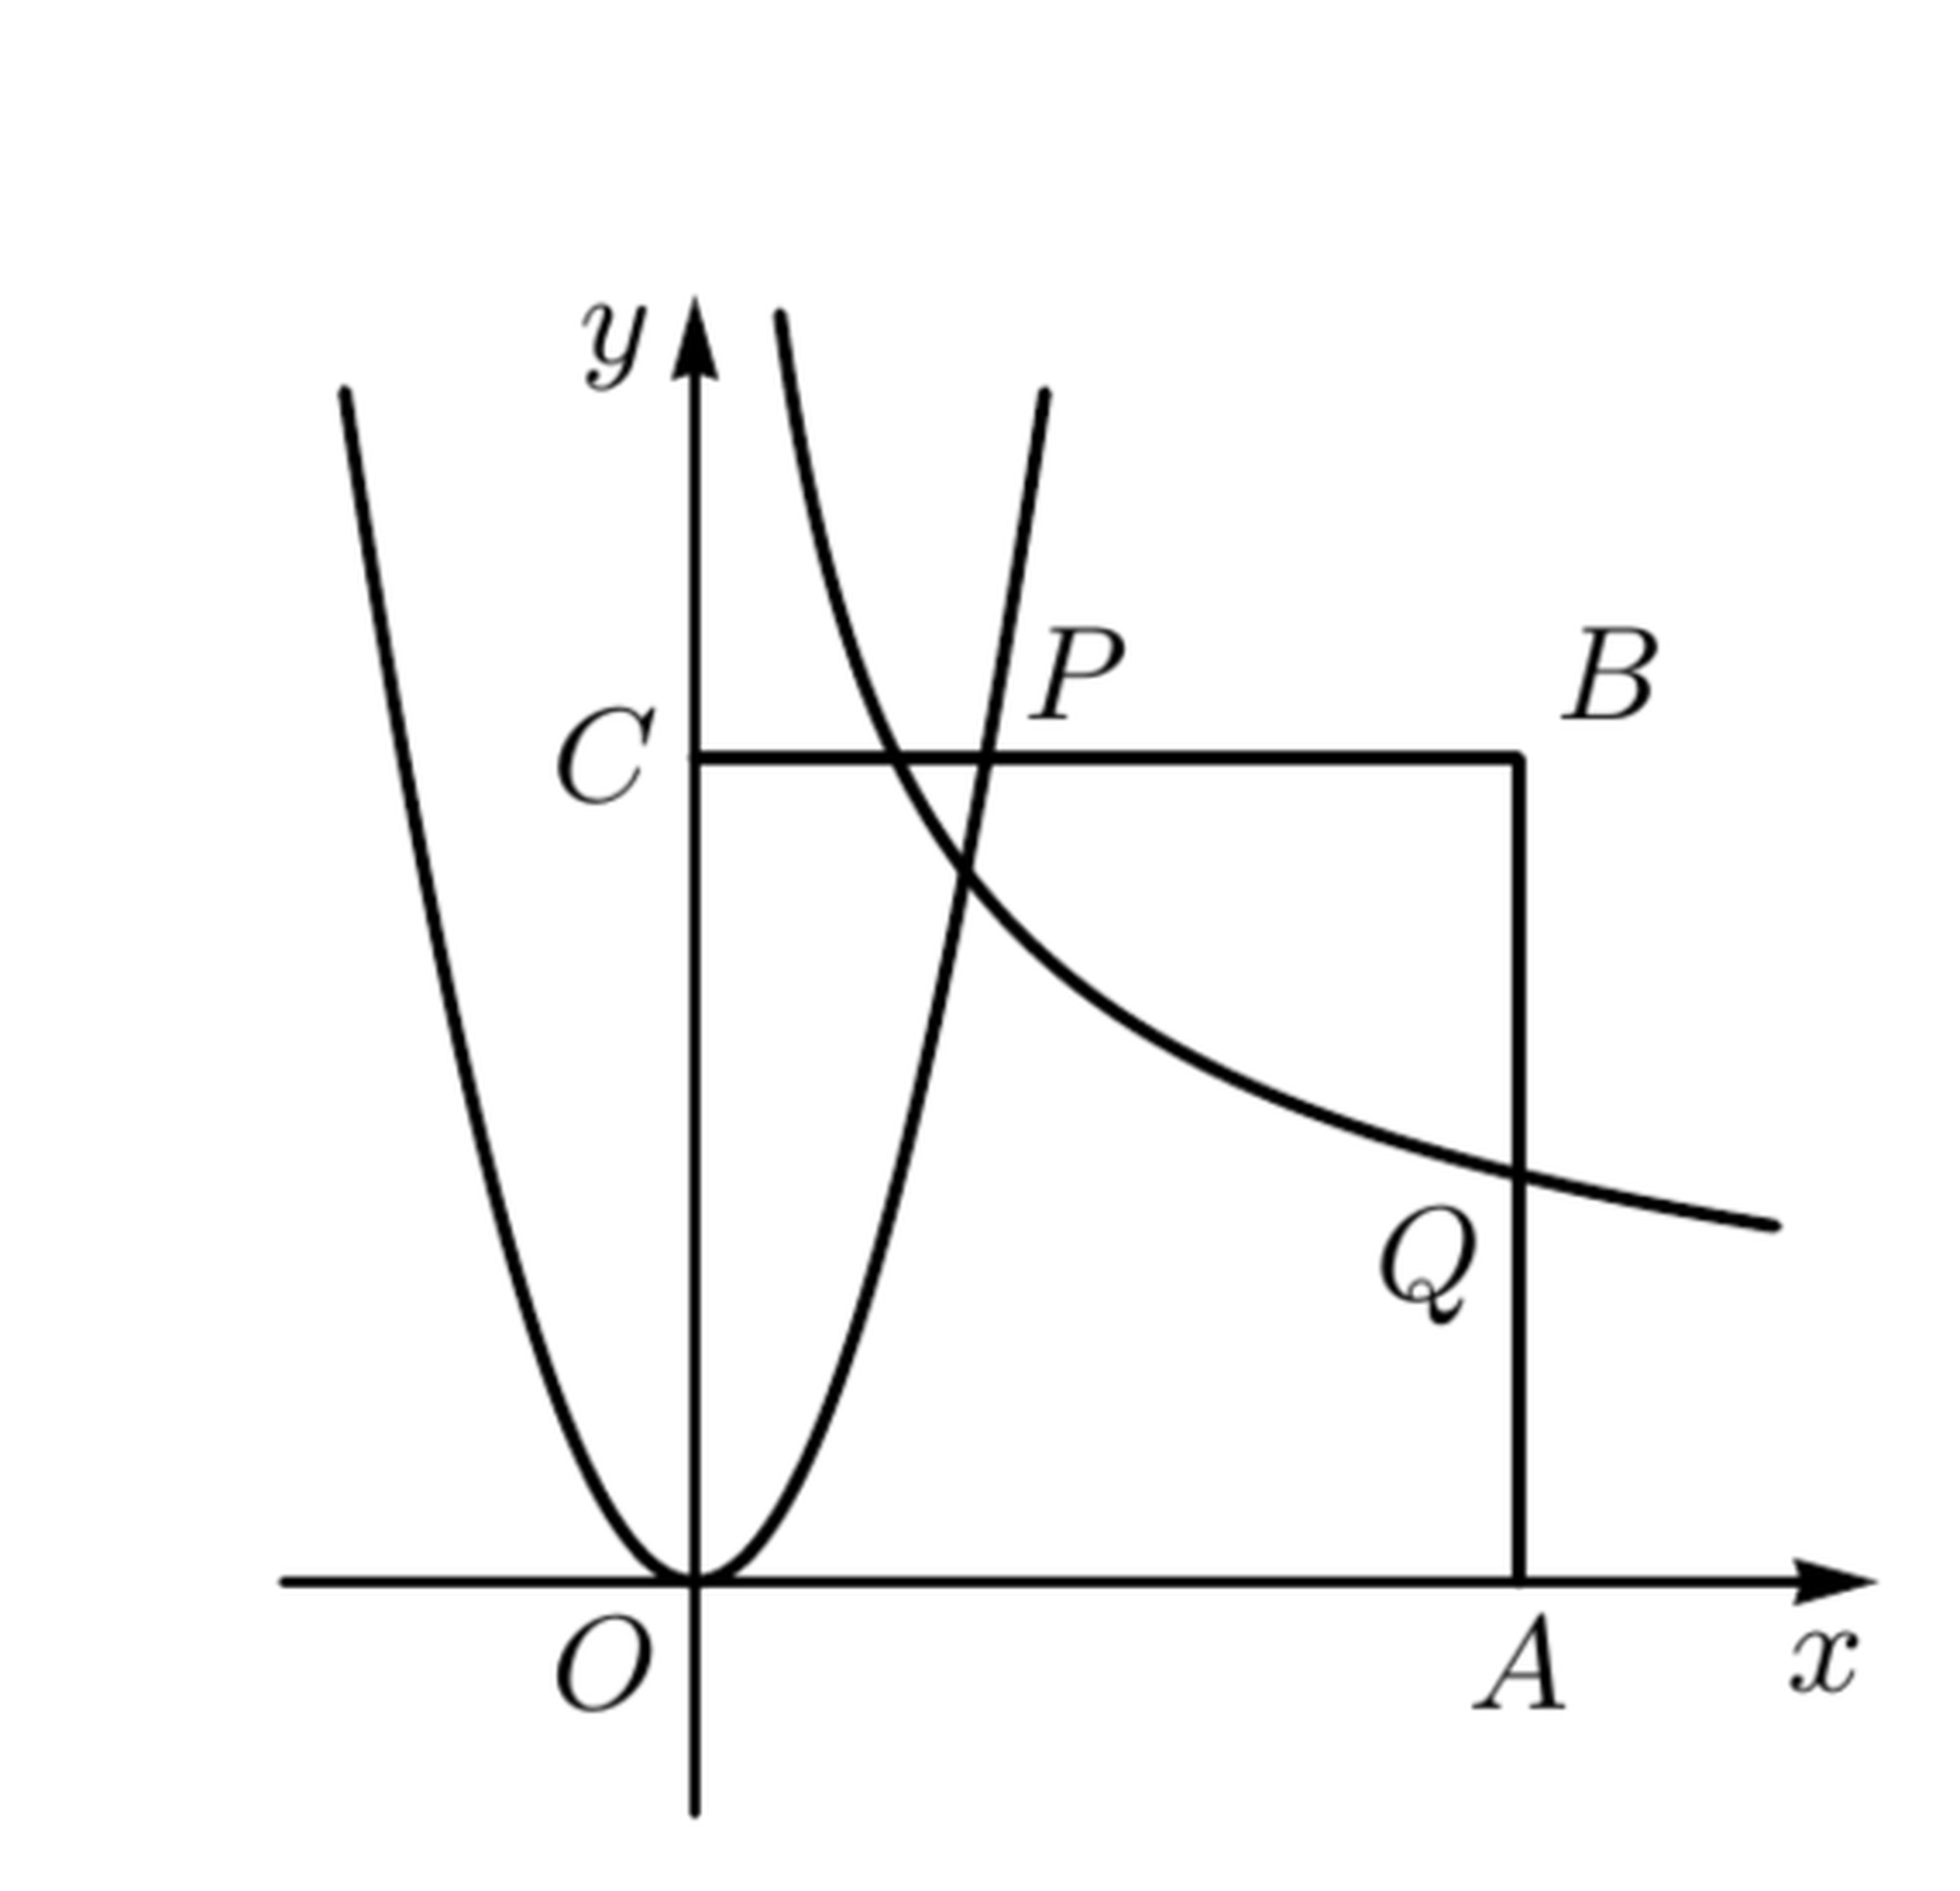
\includegraphics[width=0.40\textwidth]{figures/gao153_q11.png}
\end{center}

\ifanswer
\solbegin
\step{$\lvert AQ\rvert=\dfrac1{\sqrt a}$，$\lvert CP\rvert=\sqrt{\dfrac a5}$，}
\step{于是 $\lvert AQ\rvert+\lvert CP\rvert=\dfrac1{\sqrt a}+\sqrt{\dfrac a5}\geqslant2\sqrt{\dfrac1{\sqrt a}\cdot\sqrt{\dfrac a5}}=\dfrac2{\sqrt[4]{5}}$，}
\step{当且仅当 $\dfrac1{\sqrt a}=\sqrt{\dfrac a5}$，即 $a=\sqrt5$ 时取等号.}
\solend
\fi

% === Q12 === $B\subseteq A$ 带下划线照录、空集 \varnothing；解析 5 行
\item 若集合 $A=\{x\mid1\leqslant x\leqslant100,x\in\Z\}$，集合 $B\subseteq A$，且 $B\ne\varnothing$，记 $W(B)$ 为 $B$ 中元素的最大值与最小值之和，则对所有的 $B$，$W(B)$ 的平均值是\blankline[4.4em].

\ifanswer
\solbegin
\step{对每个非空子集 $B$，令 $B'=\{101-x\mid x\in B\}$，}
\step{则 $W(B')=(101-\min B)+(101-\max B)=202-W(B)$.}
\step{对 $B'$ 再作同样变换即得到 $B$，因此 $B$ 遍历所有非空子集时，}
\step{$B'$ 也恰好遍历所有非空子集.}
\step{设所求平均值为 $m$，则 $m=202-m$，解得 $m=101$.}
\solend
\fi

\end{enumerate}

\bigsec{二、选择题}

\begin{enumerate}
\setcounter{enumi}{12}

% === Q13 === "图像"（像，有亻）照录；解析 2 行，故选 A
\item 设 $a$、$b$ 为常数，若 $0<a<1$，$b>1$，则函数 $y=a^x-b$ 的图像必定不经过\mbox{（\quad）}

\keepwithprev
A. 第一象限\qquad\qquad B. 第二象限\qquad\qquad C. 第三象限\qquad\qquad D. 第四象限

\ifanswer
\solbegin
\step{当 $x>0$ 时，$a^x<1<b$，所以 $y=a^x-b<0$，图像必定不经过第一象限，}
\step{故选 $A$.}
\solend
\fi

% === Q14 === $m\in\Z$、中文弯引号、"图像"照录；解析 3 行，故选 A
\item 已知 $m\in\Z$，则“$m=0$”是“幂函数 $y=x^{m^2-2m-1}$ 的图像与 $x$ 轴及 $y$ 轴均无交点，且关于原点成中心对称”的\mbox{（\quad）}

\keepwithprev
A. 充分不必要条件\qquad\qquad B. 必要不充分条件

C. 充要条件\qquad\qquad D. 既不充分也不必要条件

\ifanswer
\solbegin
\step{图像满足所述条件 $\Leftrightarrow m^2-2m-1$ 为负奇数 $\Leftrightarrow m=0$ 或 $m=2$.}
\step{$m=0$ 能推出所述条件，但所述条件不能推出 $m=0$，因此是充分不必要条件，}
\step{故选 $A$.}
\solend
\fi

% === Q15 === 四选项一行；解析 5 行（跨 03→04 页），故选 D
\item 设 $a>b>1$，$x>1$，则下列不等式正确的是\mbox{（\quad）}

\keepwithprev
A. $a^x<b^x$\qquad B. $x^a<x^b$\qquad C. $\log_a x>\log_b x$\qquad D. $\log_x a>\log_x b$

\ifanswer
\solbegin
\step{$x>1$，幂函数与指数函数的单调性给出 $a^x>b^x$，$x^a>x^b$，A、B 错误.}
\step{$\log_a x=\dfrac{\lg x}{\lg a}<\dfrac{\lg x}{\lg b}=\log_b x$，C 错误.}
\step{对数函数 $y=\log_x t$ 的底数 $x>1$，在 $(0,+\infty)$ 上严格递增，}
\step{所以 $\log_x a>\log_x b$，D 正确.}
\step{故选 $D$.}
\solend
\fi

% === Q16 === $a\in\N$；解析 3 行，故选 C
\item 设 $a\in\N$，则满足不等式 $x^2-a^2x-a^2-1<0$ 的整数 $x$ 的个数不可能是\mbox{（\quad）}

\keepwithprev
A. 1\qquad\qquad B. 50\qquad\qquad C. 100\qquad\qquad D. 2026

\ifanswer
\solbegin
\step{$(x+1)(x-a^2-1)<0\Leftrightarrow-1<x<a^2+1$. 整数解为 $0,1,\cdots,a^2$，共 $a^2+1$ 个.}
\step{$1=0^2+1$，$50=7^2+1$，$2026=45^2+1$，而 $100-1=99$ 不是完全平方数，}
\step{故选 $C$.}
\solend
\fi

\end{enumerate}

\bigsec{三、解答题}

\begin{enumerate}
\setcounter{enumi}{16}

% === Q17 === 补集上划线 \overline{A}、\subseteq 照录；解析 5 行
\item 已知全集 $U=\R$，集合 $A=\{x\mid x^2-x-2\geqslant0\}$，$B=\{x\mid x>-1\}$，$C=\{x\mid a-5<x<a\}$.

(1) 求 $A\cap B$、$A\cup B$；

(2) 若 $\overline{A}\cup C=C$，求实数 $a$ 的取值范围.

\ifanswer
\solbegin
\step{(1) $x^2-x-2=(x+1)(x-2)\geqslant0\Leftrightarrow x\leqslant-1$ 或 $x\geqslant2$，}
\step{所以 $A=(-\infty,-1]\cup[2,+\infty)$，$B=(-1,+\infty)$，}
\step{因此 $A\cap B=[2,+\infty)$，$A\cup B=\R$.}
\step{(2) $\overline{A}=(-1,2)$，于是 $\overline{A}\cup C=C\Leftrightarrow\overline{A}\subseteq C\Leftrightarrow(-1,2)\subseteq(a-5,a)$，}
\step{两区间均为开区间，端点可重合，故 $\begin{cases}a-5\leqslant-1\\a\geqslant2\end{cases}\Leftrightarrow2\leqslant a\leqslant4$.}
\solend
\fi

% === Q18 === 解析 4 行
\item 已知 $a$、$b$、$c$ 都是正数，

(1) 若 $a+b=1$，求证：$\dfrac1a+\dfrac1b\geqslant4$，并指出等号成立的条件；

(2) 若 $a+b+c=1$，求证：三个数 $\dfrac1a$、$\dfrac1b$、$\dfrac1c$ 中至少有一个不小于 3.

\ifanswer
\solbegin
\step{(1) 由 $(a-b)^2\geqslant0$，得 $4ab\leqslant(a+b)^2=1$，所以 $\dfrac1a+\dfrac1b=\dfrac{a+b}{ab}=\dfrac1{ab}\geqslant4$，}
\step{等号成立当且仅当 $a=b$，结合 $a+b=1$，得 $a=b=\dfrac12$.}
\step{(2) 假设三个数 $\dfrac1a$、$\dfrac1b$、$\dfrac1c$ 都小于 3，则 $a>\dfrac13,b>\dfrac13,c>\dfrac13\Rightarrow a+b+c>1$，}
\step{与 $a+b+c=1$ 矛盾，因此三个数中至少有一个不小于 3.}
\solend
\fi

% === Q19 === 题目配图（三版都出）；\needvspace 守卫放 \item 之前；解析 19 行
\needvspace{8cm}
\item 某新建居民小区有一直角三角形绿地，两直角边长分别为 30m 和 40m，打算在其中划出一片区域改造成活动场地，如图所示.

(1) 若划出的区域为正方形，且有两边落在绿地边界上，求此正方形边长；

(2) 若划出的区域为圆形，求圆形区域面积的最大值；

(3) 若划出的区域为矩形（其中至少有一边在边界上），求此矩形面积的最大值.

\begin{center}
% 直角三角形 ABC 绿地示意图取 05 页右上，去粉色水印、去色、4× LANCZOS 放大；三版都出
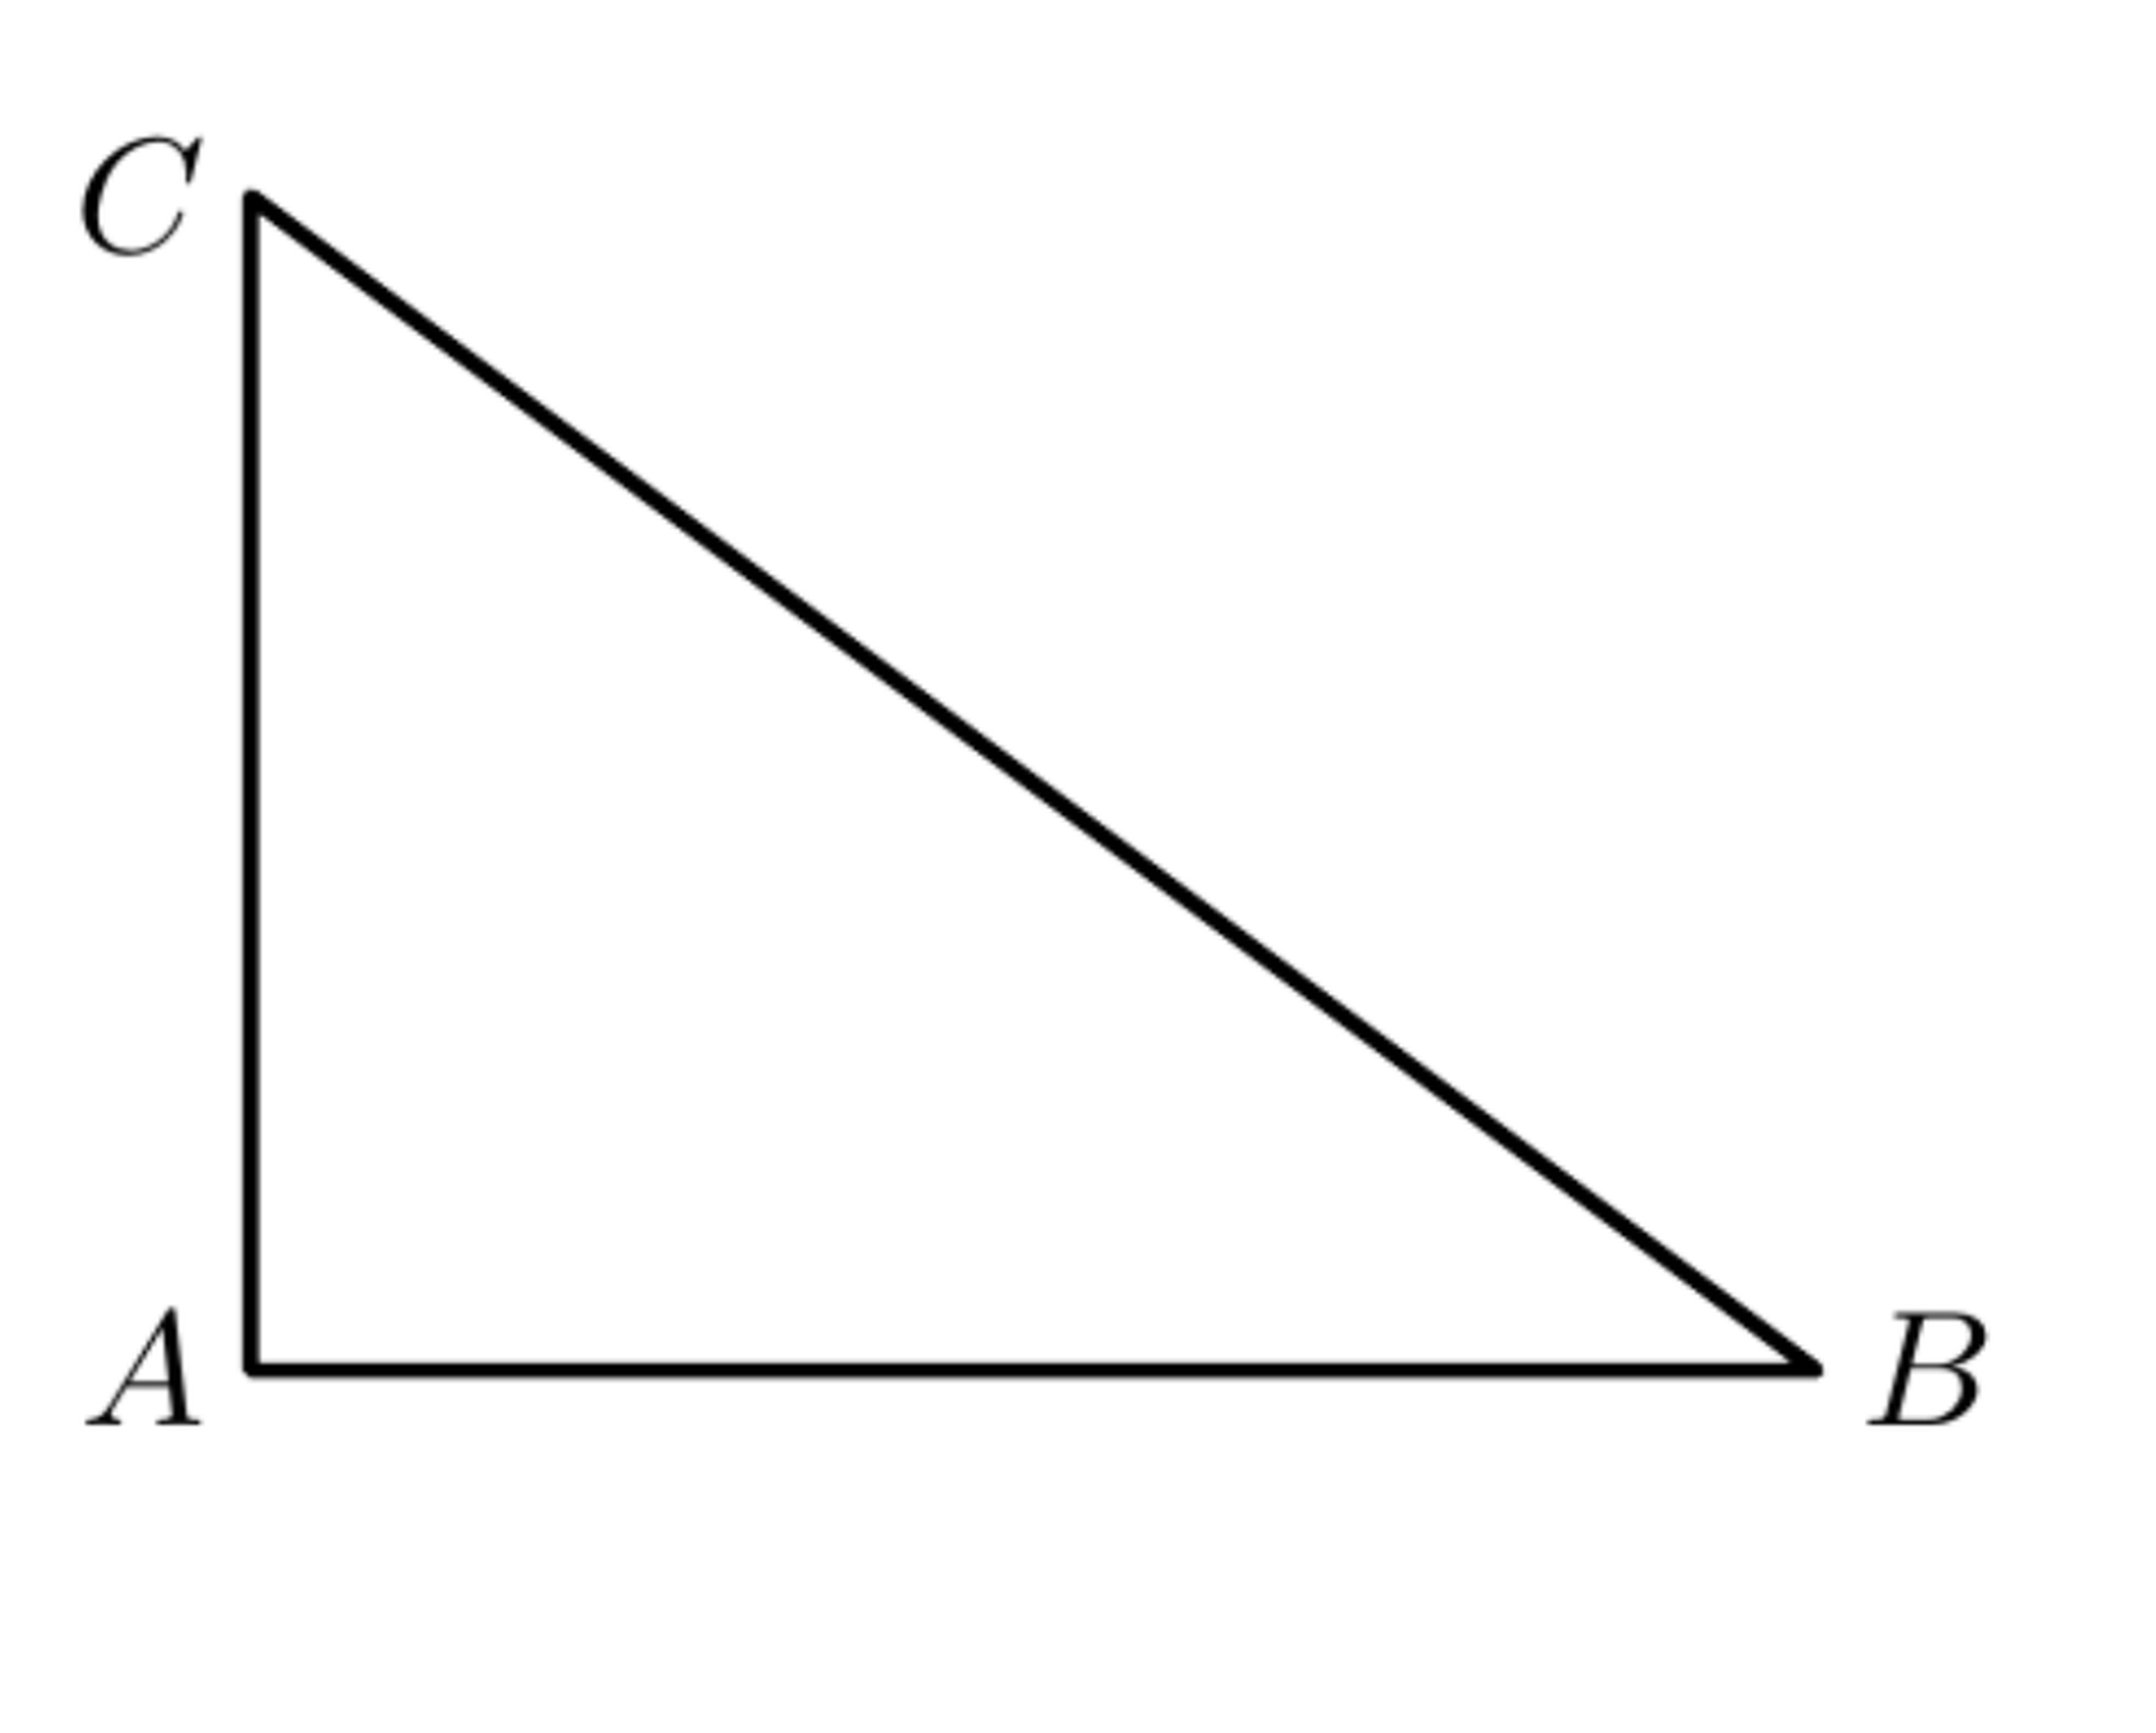
\includegraphics[width=0.34\textwidth]{figures/gao153_q19.png}
\end{center}

\ifanswer
\solbegin
\step{(1) 取 $A(0,0)$、$B(40,0)$、$C(0,30)$，则斜边 $BC$ 所在直线为 $3x+4y=120$.}
\step{正方形落在边界上的两边必分别在两条直角边上.}
\step{设其边长为 $a$m，则对角顶点为 $(a,a)$.}
\step{按题意划出的正方形应尽量大，即对角顶点落在斜边 $BC$ 上，}
\step{因此 $3a+4a=120\Rightarrow a=\dfrac{120}{7}$；}
\step{(2) 斜边长 $BC=\sqrt{30^2+40^2}=50$m，三角形面积为 $600\text{m}^2$.}
\step{设圆的半径为 $r$，圆心到 $AB$、$AC$、$BC$ 的距离分别为 $d_1,d_2,d_3$，}
\step{则三者均不小于 $r$. 连接圆心与三个顶点，}
\step{得 $600=\dfrac12(40d_1+30d_2+50d_3)\geqslant\dfrac12(40+30+50)r=60r$，所以 $r\leqslant10$.}
\step{取三角形的内切圆时等号成立，圆形区域面积的最大值为 $100\pi\text{m}^2$.}
\step{(3) 任取矩形落在绿地边界上的一边，以其所在直线为横轴.}
\step{设相应三角形底边长为 $L$、高为 $H$，则 $LH=1200$.}
\step{取三角形顶点坐标为 $(0,0)$、$(L,0)$、$(p,H)$.}
\step{在高度 $t$ 处，两腰上的点的横坐标分别为 $\dfrac{pt}{H}$、$L+\dfrac{(p-L)t}{H}$，}
\step{因此，高为 $t$ 的矩形，其底边长不超过 $L\left(1-\dfrac tH\right)$，}
\step{面积满足 $S\leqslant Lt\left(1-\dfrac tH\right)=\dfrac LH\left[\dfrac{H^2}{4}-\left(t-\dfrac H2\right)^2\right]\leqslant\dfrac{LH}{4}=300$，}
\step{在原坐标系中，取矩形顶点为 $(0,0)$、$(20,0)$、$(20,15)$、$(0,15)$，}
\step{其中 $3\times20+4\times15=120$，矩形完全位于绿地内，面积为 $300\text{m}^2$，}
\step{达到最大值.}
\solend
\fi

% === Q20 === $g(x)$ 定义照录；解析 14 行
\item 已知 $a>0$ 且 $a\ne1$，设 $f(x)=\log_a(x^2-a^2)$，$g(x)=2\log_a(x-ak)$.

(1) 求函数 $y=f(x)$ 的定义域；

(2) 若 $k=2$，求不等式 $f(x)>g(x)$ 的解集；

(3) 若“存在实数 $x$，使得 $f(x)=g(x)$”为真命题，求实数 $k$ 的取值范围.

\ifanswer
\solbegin
\step{(1) $x^2-a^2>0\Leftrightarrow x<-a$ 或 $x>a$，定义域为 $(-\infty,-a)\cup(a,+\infty)$.}
\step{(2) 两函数均有意义时，$x>2a$，且 $g(x)=\log_a(x-2a)^2$.}
\step{当 $a>1$ 时，$f(x)>g(x)\Leftrightarrow x^2-a^2>(x-2a)^2\Leftrightarrow x>\dfrac{5a}{4}$，}
\step{结合 $x>2a$，解集为 $(2a,+\infty)$.}
\step{当 $0<a<1$ 时，$f(x)>g(x)\Leftrightarrow x^2-a^2<(x-2a)^2\Leftrightarrow x<\dfrac{5a}{4}$，}
\step{与 $x>2a$ 矛盾，解集为 $\varnothing$.}
\step{(3) 在 $x^2-a^2>0$ 且 $x-ak>0$ 的条件下，}
\step{$f(x)=g(x)\Leftrightarrow x^2-a^2=(x-ak)^2\Leftrightarrow2akx=a^2(1+k^2)$，}
\step{当 $k=0$ 时，上式不成立；}
\step{当 $k\ne0$ 时，$x=\dfrac{a(1+k^2)}{2k}$，}
\step{于是 $x-ak=\dfrac{a(1-k^2)}{2k}>0\Leftrightarrow k<-1$ 或 $0<k<1$，}
\step{对上述 $k$，所取的 $x$ 同时满足 $x^2-a^2=(x-ak)^2>0$，}
\step{两函数均有意义且函数值相等.}
\step{因此，$k$ 的取值范围为 $(-\infty,-1)\cup(0,1)$.}
\solend
\fi

% === Q21 === 中文弯引号、复杂式照录；解析 23 行（跨 08→09 页）
\item 若实数 $x$、$y$、$m$ 满足 $\lvert x-m\rvert<\lvert y-m\rvert$，则称 $x$ 比 $y$ 接近 $m$.

(1) 若 $2x$ 比 $x-2$ 更接近 1，求实数 $x$ 的取值范围；

(2) 若 $x$ 比 $y$ 接近 $m$，证明：“$x>y$” 的充要条件是 “$x+y<2m$”；

(3) 已知 $x>0$，$y>0$ 且 $x\ne y$. 设 $p=\dfrac{x^2+y^2}{xy}$，若对于任意的 $x$、$y$，命题 “$p$ 比 $p^2-3p+4$ 接近 $m$” 恒成立，求实数 $m$ 的取值范围.

\ifanswer
\solbegin
\step{(1) $\lvert2x-1\rvert<\lvert x-3\rvert\Leftrightarrow(2x-1)^2<(x-3)^2\Leftrightarrow(x+2)(3x-4)<0$，}
\step{解得 $-2<x<\dfrac43$，实数 $x$ 的取值范围为 $\left(-2,\dfrac43\right)$.}
\step{(2) 因为 $x$ 比 $y$ 接近 $m$，所以 $\lvert x-m\rvert<\lvert y-m\rvert$，则 $\lvert x-m\rvert^2<\lvert y-m\rvert^2$，}
\step{即 $(x-m)^2<(y-m)^2$，即 $(x-m)^2-(y-m)^2<0$，}
\step{即得 $(x-y)(x+y-2m)<0$，}
\step{则由 $x+y<2m$，得 $x+y-2m<0$，}
\step{故 $x-y>0$，即 $x>y$，充分性成立；}
\step{当 $x>y$ 时，$x-y>0$，结合 $(x-y)(x+y-2m)<0$，得 $x+y-2m<0$，}
\step{即 $x+y<2m$，必要性成立；}
\step{故“$x>y$” 的充要条件是 “$x+y<2m$”；}
\step{(3) $x>0$，$y>0$ 且 $x\ne y$. 则 $p=\dfrac{x^2+y^2}{xy}=\dfrac xy+\dfrac yx>2\sqrt{\dfrac xy\cdot\dfrac yx}=2$，}
\step{由于对于任意的 $x$、$y$，命题 “$p$ 比 $p^2-3p+4$ 接近 $m$” 恒成立，}
\step{故 $\lvert p-m\rvert<\lvert(p^2-3p+4)-m\rvert$ 对 $\forall p>2$ 恒成立，}
\step{即得 $(p-m)^2<(p^2-3p+4-m)^2$，}
\step{即 $(p^2-3p+4-m)^2-(p-m)^2>0$，}
\step{得 $(p^2-4p+4)(p^2-2p+4-2m)>0$，}
\step{即 $(p-2)^2(p^2-2p+4-2m)>0$，由于 $p>2$，故 $(p-2)^2>0$，}
\step{故 $p^2-2p+4-2m>0$ 对 $\forall p>2$ 恒成立，}
\step{即 $2m<p^2-2p+4$ 对 $\forall p>2$ 恒成立，}
\step{由于 $p^2-2p+4=(p-1)^2+3$，此时 $p^2-2p+4$ 在 $(2,+\infty)$ 上严格增，}
\step{故 $(p-1)^2+3>(2-1)^2+3=4$，故 $2m\leqslant4$，解得 $m\leqslant2$，}
\step{即实数 $m$ 的取值范围是 $(-\infty,2]$.}
\solend
\fi

\end{enumerate}

\end{document}
"
%
% ① 原始材料：微信公众号"魔都数学加油站"文章，连载"27学年高一153"，原文标题
% "27学年高一153——2026-2027年上海市闵行中学文绮中学高一上期中"；
% 原文链接：https://mp.weixin.qq.com/s/rEtS-92cDR6JKgY2b5DRfg 。
% 正文为 9 张 PNG 页（01/02/06/07/08/09 为 2560×3620，03/04/05 为 4762×6735，
% 同一篇各页分辨率混排，逐页按各自分辨率裁图核对，别按预览比例换算裁框）。
% 体例：讲评版——填空 3—12（10 题）、选择 13—16（4 题）、解答 17—21（5 题），
% 共 19 题，自第 3 题起编；**全 19 题均印【解析】**（逐题核实，见 ② ②）。
% 题目、答案、解析均据原图转录；卷面粉红色水印"魔都数学加油站"及公众号页脚未录入。
% 全卷插图清单（逐页通读 9 页确认）：2 幅，均为题目配图、三版都出——
%   · Q11 正方形 OABC 曲线图（02 页右下：$y=5x^2$ 与 $y=x^{-\frac12}$ 两条曲线、
%     坐标轴、O/A/B/C/P/Q、正方形），裁 figures/gao153_q11.png；
%   · Q19 直角三角形 ABC 绿地示意图（05 页右上，直角在 A），
%     裁 figures/gao153_q19.png；
%   两图均去粉色水印、去色、4× LANCZOS 放大；Q11 图左上角题干残字"函"已裁白。
%   其余各页逐页确认无其它题目配图、无解析内配图、无表格；09 页下半仅水印、无正文。
%
% 卷首标题：原卷印作"2026-2027 年闵行中学文绮中学高一上期中"，年份区间按全稿惯例排 en dash；
% 原卷卷面未印副标题，本稿按同期中卷知识模块口径补出"集合与常用逻辑用语、不等式、函数"。
%
% ② 与原卷的排版差异：
%   ① 原文从第 3 题起，本稿保留原题号；共 19 题三节，解答题 5 题到 21；
%   ② 全 19 题均印【解析】、用 \solbegin…\solend，无只印【答案】或答案印括号内的题；
%      四道选择题答案在解析末句"故选 A／A／D／C"（Q13—Q16，逐个放大复核）、
%      括号 \mbox{（\quad）} 留空、不另提 \ans{}；答案版【答案】/【解析】标记数
%      = 19 = 全卷题数；
%   ③ 原卷卷面未印副标题，本稿按知识模块口径补出；
%   ④ 原卷填空横线按全稿惯例排 \blankline[4.4em]；选择题括号排 \mbox{（\quad）}、
%      四道选择题的选项段前按惯例各加 \keepwithprev；解答题不留作答区、不加
%      \anspace（原卷为讲评版，109—113 起全稿不用 \anspace）；
%   ⑤ 数集：Q3"$x\in R$"、Q5"解集为 R"、Q10"$x\in N$"、Q12"$x\in Z$"与
%      "$m\in Z$"、Q14"$m\in Z$"、Q16"$a\in N$"、Q17"全集 $U=R$"、
%      Q19 无、Q21 无——原卷印斜体或正体粗体 R/N/Z，按全稿惯例归一
%      \R／\N／\Z；绝对值排 \lvert…\rvert（Q5、Q11、Q21），集合描述竖线排 \mid
%      （Q3、Q10、Q17、Q20），不等号按全稿惯例排 \leqslant／\geqslant；
%      补集照原卷上划线排 \overline{A}（Q17 题干 (2)＋解析 (2)）；
%      空集 \varnothing（Q12 题干、Q20 解析 (2)）；子集 3 处均印带下划线 ⊆、
%      照录 \subseteq（Q10 $A\subseteq U$、Q12 $B\subseteq A$、Q17 $(-1,2)\subseteq(a-5,a)$），
%      本卷无单线 \subset 用例；
%   ⑥ 判别式：逐页通读 9 页，本卷无一元二次判别式 Δ/△ 算式，故无 Δ/△ 混用可照录；
%      Q11 图里有几何正方形 OABC（非三角形符号），无 △ABC 用例；
%   ⑦ 中文弯引号照录：Q14"$m=0$"与"幂函数…关于原点成中心对称"、
%      Q20"存在实数 $x$，使得 $f(x)=g(x)$"、Q21"$x>y$"与"$x+y<2m$"、
%      "$p$ 比 $p^2-3p+4$ 接近 $m$"（引号外留空格按原卷）；
%      注释里一律 ASCII 引号；数学式内 CJK 用 \text{}；
%   ⑧ "图像／图象"逐处放大核：全卷 3 处均印"图像"（像，有亻）——
%      Q13 题干与解析、Q14 题干与解析；Q19 题干写"如图所示"（非"图像"），
%      逐处照录未统一；子题标号 (1)(2)(3) 半角括号照录；圈数字本卷无用例；
%   ⑨ 半角逗号在数学组之间是全稿惯例、非笔误，逐处照录（Q3 $x\in R$、
%      Q10 $a_1,a_2$、Q19 $A(0,0)$、$d_1,d_2,d_3$、Q21 $a>\frac13,b>\frac13$ 等）；
%      行末西文句点 ASCII `.`；行中全角逗号／顿号照录（Q19"30m 和 40m"、
%      Q21"实数 $x$、$y$、$m$"）；
%   ⑩ 复杂式照录别简化：Q3 $y=x^{-2}$、Q11 $y=x^{-\frac12}$ 与
%      $\frac{2}{\sqrt[4]{5}}$、Q8 $\frac{2b}{a+1-b}$、Q9 cases 块、
%      Q10 $525=5\times105$、Q16 $a^2+1$、Q19 $S\leqslant Lt(1-\frac tH)$
%      与 $L+\frac{(p-L)t}{H}$、Q20 $2akx=a^2(1+k^2)$ 与 $\frac{a(1+k^2)}{2k}$、
%      Q21 $(p^2-4p+4)(p^2-2p+4-2m)>0$；
%      \left…\right 不得拆到不同 $…$ 组（Q17 $\left\{x\mid\cdots\right\}$、
%      Q19 $\left[\frac{H^2}{4}-\left(t-\frac H2\right)^2\right]$、
%      Q21 $\left(-2,\frac43\right)$ 等）；cases 块一律 \begin{cases}…\end{cases}；
%   ⑪ 一条 \step = 原卷解析的一个印刷行，cases 块整体算一个印刷行；别并折行、
%      别拆行。Q10 六行、Q19 十九行、Q20 十四行、Q21 二十二行均按印刷行逐条断，
%      不丢行；
%   ⑫ 配图：Q11／Q19 题目配图（三版都出）放 \item 内题干之后 \begin{center}，
%      各用 \needvspace{8cm} 守卫把整块推走，**守卫放在 \item 之前**
%      （见 高一145 Q14/Q20 成例与切页审计 B 类坑）；
%   ⑬ 原卷解析内无红色"法一／法二"之类小标题，故本卷无 \stepm；红色水印
%      "魔都数学加油站"不录入；
%   ⑭ 跨页续印按题合并：见 ⑥；
%
% ③ 行数复核：一条 \step = 原卷解析的一个印刷行，cases 块作一个印刷行计。
%   逐题数（主会话逐页核对定稿）：Q3：1；Q4：2；Q5：2；Q6：2；Q7：1；
%   Q8：1；Q9：2；Q10：6；Q11：3；Q12：5；Q13：2；Q14：3；Q15：5；
%   Q16：3；Q17：5；Q18：4；Q19：19；Q20：14；Q21：22。
%   合计 102 条 \step（本卷无 \stepm），与原卷逐题印刷行相等。全卷 19 题
%   均设 \solbegin…\solend，答案版【答案】/【解析】标记数 = 19 = 全卷题数。
%
% ④ 判别式／子集符号结论（逐处放大原图照录、不得统一，主会话像素级复核）：
%   判别式：逐页通读 9 页，本卷无一元二次判别式算式（Q7 用韦达定理、
%      Q16 用因式分解、Q20 用对数方程，均不写 Δ/△），故无 Δ/△ 混用可照录
%      （"高 \Delta／扁 \triangle"口径备查，参照 高一142／151／152 头注）；
%      本卷无几何三角形符号用例。
%   子集：Q10 题干"$A\subseteq U$"、Q12 题干"$B\subseteq A$"、Q17 解析 (2)
%      "$(-1,2)\subseteq(a-5,a)$"共 3 处，逐处放大确认均印带下划线 ⊆、
%      照录 \subseteq；本卷未见单线 ⊂（\subset）之对应处。
%      补集上划线 \overline{A}（Q17）、空集 \varnothing（Q12 题干、Q20 解析 (2)）；
%      数集 \R／\N／\Z 归一见 ② ⑤。
%
% ⑤ 存疑照录（放大原图确认，照录未改、正文对应处另有 % 注）：
%   1. Q3 集合 $B=\{(x,y)\mid y=x^{-2},x\in\R\}$ 原卷题干径写 $x\in\R$
%      （$x=0$ 处无意义），解析自行注明 $x\ne0$，照录未改。
%   2. Q10 解析"$U$ 中共有 $525=5\times105$ 个连续整数"与尾行
%      "取 $U$ 中除以 5 余 1 或 2 的全部元素及元素 5"逐字照录（放大 02 页
%      /tmp/gao153/z/zoom/q10_pick.png 确认是"元素 5"，非"元素 9"）。
%   3. Q11 第二个函数原卷印 $y=x^{-\frac12}$（负二分之一次幂，非 $x^2$），
%      放大 02 页 /tmp/gao153/z/zoom/q11_exp.png 确认，照录未改；
%      $|AQ|=\frac1{\sqrt a}$ 与之自洽。
%   4. Q19 (3) 解析"在高度 $t$ 处，两腰上的点的横坐标分别为 $\frac{pt}{H}$、
%      $L+\frac{(p-L)t}{H}$"，放大 06 页确认，照录未简化。
%   5. Q20 (2) 解析"$g(x)=\log_a(x-2a)^2$"（真数整体平方），
%      与 $g(x)=2\log_a(x-ak)$ 在 $k=2$ 时一致，照录未改。
%   6. Q21 (3) 解析"得 $(p^2-4p+4)(p^2-2p+4-2m)>0$"与
%      "故 $(p-1)^2+3>(2-1)^2+3=4$，故 $2m\leqslant4$"照录未改
%      （放大 09 页 /tmp/gao153/z/zoom/q21_factor.png 确认）。
%   7. "图像／图象"全卷 3 处均印"图像"（像，有亻）逐处照录；
%      本卷无判别式 Δ/△ 用例（见 ④）。
%   全卷除此 7 类外未发现其它笔误／自相矛盾处；19 题均印【解析】、
%   无只印【答案】或答案印括号内的题（见 ② ②）。
%
% ⑥ 跨页续印按题合并说明（逐页核实定稿）：Q3—Q5 题干＋解析在 01 页；
%   Q6—Q8 题干＋解析在 01 页下半（Q8 解析续 02 页顶）；Q9 题干＋解析、
%   Q10 题干＋解析首 2 行在 02 页上半，Q10 解析余 4 行在 02 页下半；
%   Q11 题干＋配图＋解析、Q12 题干＋解析 5 行在 02 页下半—03 页上半；
%   "二、选择题"标题在 03 页中部；Q13 题干＋选项＋解析在 03 页下半；
%   Q14 题干＋选项＋解析、Q15 题干＋选项＋解析首行在 03 页下半—04 页顶；
%   Q15 解析余 4 行、Q16 题干＋选项＋解析在 04 页上半；"三、解答题"
%   标题在 04 页下半；Q17 题干＋两问＋解析 5 行在 04 页下半—05 页顶；
%   Q18 题干＋两问＋解析 4 行、Q19 题干（含配图）＋三问在 05 页；
%   Q19 解析 (1)(2) 9 行在 05 页下半，解析 (3) 前 5 行在 06 页上半、
%   余 4 行在 06 页下半；Q20 题干＋三问在 06 页下半，解析 (1)(2)(3)
%   前 6 行在 07 页上半、(3) 余 8 行在 07 页下半；Q21 题干＋三问在
%   07 页末，解析 (1)(2) 10 行在 08 页上半—下半，解析 (3) 前 4 行在
%   08 页下半、余 9 行续 09 页上半，末行"即实数 $m$ 的取值范围是
%   $(-\infty,2]$"为全卷收尾（09 页下半仅水印、无正文）。
%   本稿按题连排，不丢行、不并折行；全卷末题为第 21 题，无附加题节。
%
\documentclass[a4paper,11pt]{article}
\usepackage{common}

\begin{document}

\examtitlest[3]{2026--2027 年闵行中学文绮中学高一上期中}{集合与常用逻辑用语、不等式、函数}

\bigsec{一、填空题}

\begin{enumerate}
\setcounter{enumi}{2}

% === Q3 === 集合描述竖线 \mid；$y=x^{-2}$ 照录；解析 1 行
\item 已知 $A=\{(x,y)\mid y=x^3,x\in\R\}$，$B=\{(x,y)\mid y=x^{-2},x\in\R\}$，则 $A\cap B=$\blankline[4.4em].

\ifanswer
\solbegin
\step{$x^3=x^{-2}\ (x\ne0)\Leftrightarrow x^5=1\Leftrightarrow x=1$，此时 $y=1$，所以 $A\cap B=\{(1,1)\}$.}
\solend
\fi

% === Q4 === 解析 2 行
\item 若关于 $x$ 的不等式 $\dfrac{x-a}{x+1}>0$ 的解集为 $(-\infty,-1)\cup(4,+\infty)$，则实数 $a=$\blankline[4.4em].

\ifanswer
\solbegin
\step{关于 $x$ 的不等式 $\dfrac{x-a}{x+1}>0$ 即 $(x+1)(x-a)>0$.}
\step{再由它的解集为 $(-\infty,-1)\cup(4,+\infty)$，得 $-1$ 和 4 是 $(x+1)(x-a)=0$ 的两个实数根，故 $a=4$.}
\solend
\fi

% === Q5 === 绝对值 \lvert…\rvert；解析 2 行
\item 若关于 $x$ 的不等式 $\lvert x+1\rvert+\lvert x-2\rvert>m$ 的解集为 $\R$，则实数 $m$ 的取值范围是\blankline[4.4em].

\ifanswer
\solbegin
\step{$\lvert x+1\rvert+\lvert x-2\rvert\geqslant\lvert(x+1)-(x-2)\rvert=3$，当且仅当 $-1\leqslant x\leqslant2$ 时取等号，}
\step{因此 $m<3$.}
\solend
\fi

% === Q6 === 解析 2 行
\item 已知指数函数 $y=a^x$（$a>1$）在区间 $[-1,1]$ 上的最大值比最小值大 $\dfrac32$，则实数 $a=$\blankline[4.4em].

\ifanswer
\solbegin
\step{$a>1$，指数函数在 $[-1,1]$ 上严格增，故 $a-\dfrac1a=\dfrac32\Leftrightarrow(a-2)(2a+1)=0$.}
\step{结合 $a>1$，得 $a=2$.}
\solend
\fi

% === Q7 === 韦达定理；解析 1 行
\item 已知关于 $x$ 的一元二次方程 $x^2+px+2p=0$ 的两个实数根分别为 $x_1$、$x_2$，且 $(x_1+1)(x_2+1)=0$，则 $p=$\blankline[4.4em].

\ifanswer
\solbegin
\step{$0=(x_1+1)(x_2+1)=x_1x_2+x_1+x_2+1=2p-p+1=p+1\Rightarrow p=-1$.}
\solend
\fi

% === Q8 === 换底公式；解析 1 行
\item 已知 $10^a=3$，$\lg5=b$，则 $\log_6 25=$\blankline[4.4em]（用关于 $a,b$ 的关系式表示）.

\ifanswer
\solbegin
\step{$\lg3=a$，$\lg2=1-b$，所以 $\log_6 25=\dfrac{\lg25}{\lg6}=\dfrac{2b}{a+1-b}$.}
\solend
\fi

% === Q9 === cases 块整体算一个印刷行；解析 2 行
\item 已知 $A=[2,5]$，若对任意 $x\in A$，总有 $\dfrac{k}{x}\in A$，则正数 $k=$\blankline[4.4em].

\ifanswer
\solbegin
\step{$k>0$，当 $x\in[2,5]$ 时，$\dfrac{k}{x}$ 的取值范围为 $\left[\dfrac k5,\dfrac k2\right]$，}
\step{因此 $\begin{cases}\dfrac k5\geqslant2\\\dfrac k2\leqslant5\end{cases}\Leftrightarrow10\leqslant k\leqslant10\Leftrightarrow k=10$.}
\solend
\fi

% === Q10 === $A\subseteq U$ 带下划线照录；解析 6 行
\item 已知集合 $U=\{x\mid4\leqslant x\leqslant528,x\in\N\}$，$A=\{a_1,a_2,a_3,\cdots,a_n\}$，且 $A\subseteq U$. 如果集合 $A$ 中的任意两个不同元素之和都不能被 5 整除，则正整数 $n$ 的最大值为\blankline[4.4em].

\ifanswer
\solbegin
\step{$U$ 中共有 $525=5\times105$ 个连续整数，按除以 5 的余数分成五类，}
\step{每类均有 105 个元素.}
\step{余数为 1,4 的两类不能同时选取，余数为 2,3 的两类也不能同时选取，}
\step{余数为 0 的一类最多选 1 个，因此 $n\leqslant105+105+1=211$.}
\step{取 $U$ 中除以 5 余 1 或 2 的全部元素及元素 5，}% 放大 02 页确认是「元素 5」（非 9），照录未改（见 ⑤ 2）
\step{任意两个不同元素之和均不能被 5 整除，此时 $n=211$，最大值为 211.}
\solend
\fi

% === Q11 === 题目配图（三版都出）；\needvspace 守卫放 \item 之前；$y=x^{-\frac12}$ 照录；解析 3 行
\needvspace{8cm}
\item 如图，已知正方形 $OABC$，其中 $OA=a$（$a>1$），函数 $y=5x^2$ 交 $BC$ 于点 $P$，函数 $y=x^{-\frac12}$ 交 $AB$ 于点 $Q$，当 $\lvert AQ\rvert+\lvert CP\rvert$ 最小时，$a$ 的值为\blankline[4.4em].

\begin{center}
% 正方形 OABC 与两条曲线图取 02 页右下，去粉色水印、去色、4× LANCZOS 放大；三版都出
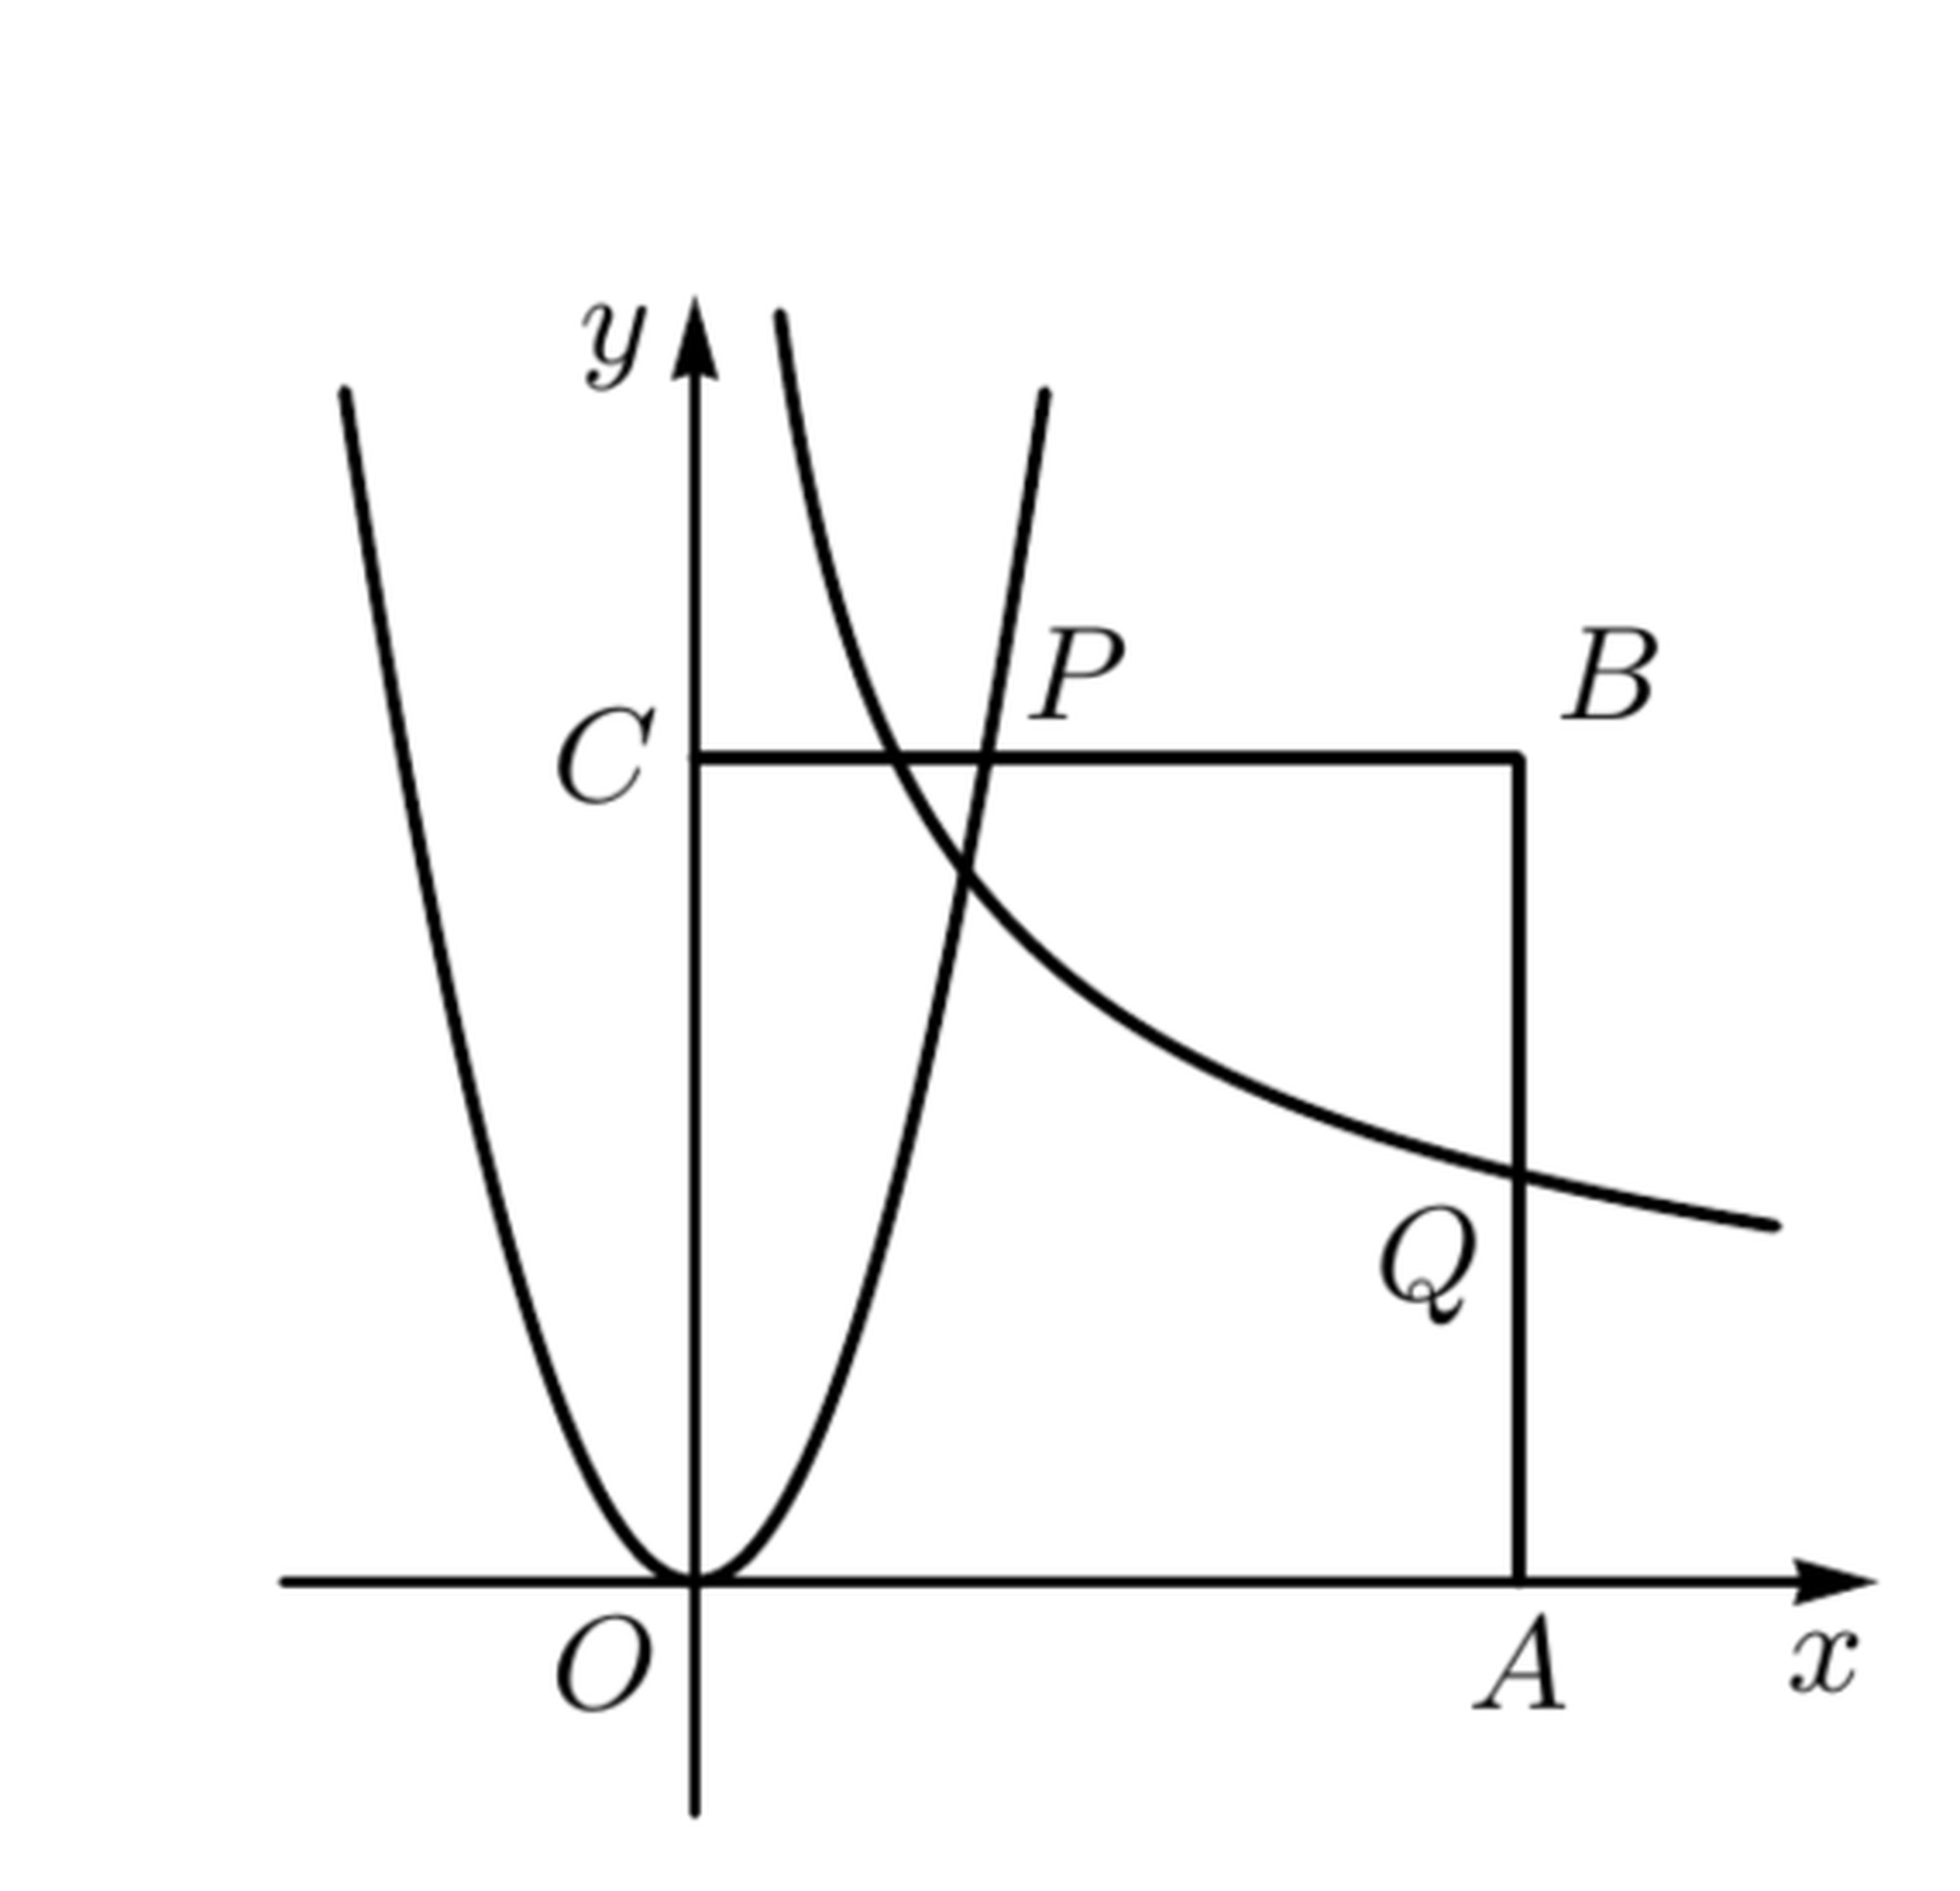
\includegraphics[width=0.40\textwidth]{figures/gao153_q11.png}
\end{center}

\ifanswer
\solbegin
\step{$\lvert AQ\rvert=\dfrac1{\sqrt a}$，$\lvert CP\rvert=\sqrt{\dfrac a5}$，}
\step{于是 $\lvert AQ\rvert+\lvert CP\rvert=\dfrac1{\sqrt a}+\sqrt{\dfrac a5}\geqslant2\sqrt{\dfrac1{\sqrt a}\cdot\sqrt{\dfrac a5}}=\dfrac2{\sqrt[4]{5}}$，}
\step{当且仅当 $\dfrac1{\sqrt a}=\sqrt{\dfrac a5}$，即 $a=\sqrt5$ 时取等号.}
\solend
\fi

% === Q12 === $B\subseteq A$ 带下划线照录、空集 \varnothing；解析 5 行
\item 若集合 $A=\{x\mid1\leqslant x\leqslant100,x\in\Z\}$，集合 $B\subseteq A$，且 $B\ne\varnothing$，记 $W(B)$ 为 $B$ 中元素的最大值与最小值之和，则对所有的 $B$，$W(B)$ 的平均值是\blankline[4.4em].

\ifanswer
\solbegin
\step{对每个非空子集 $B$，令 $B'=\{101-x\mid x\in B\}$，}
\step{则 $W(B')=(101-\min B)+(101-\max B)=202-W(B)$.}
\step{对 $B'$ 再作同样变换即得到 $B$，因此 $B$ 遍历所有非空子集时，}
\step{$B'$ 也恰好遍历所有非空子集.}
\step{设所求平均值为 $m$，则 $m=202-m$，解得 $m=101$.}
\solend
\fi

\end{enumerate}

\bigsec{二、选择题}

\begin{enumerate}
\setcounter{enumi}{12}

% === Q13 === "图像"（像，有亻）照录；解析 2 行，故选 A
\item 设 $a$、$b$ 为常数，若 $0<a<1$，$b>1$，则函数 $y=a^x-b$ 的图像必定不经过\mbox{（\quad）}

\keepwithprev
A. 第一象限\qquad\qquad B. 第二象限\qquad\qquad C. 第三象限\qquad\qquad D. 第四象限

\ifanswer
\solbegin
\step{当 $x>0$ 时，$a^x<1<b$，所以 $y=a^x-b<0$，图像必定不经过第一象限，}
\step{故选 $A$.}
\solend
\fi

% === Q14 === $m\in\Z$、中文弯引号、"图像"照录；解析 3 行，故选 A
\item 已知 $m\in\Z$，则“$m=0$”是“幂函数 $y=x^{m^2-2m-1}$ 的图像与 $x$ 轴及 $y$ 轴均无交点，且关于原点成中心对称”的\mbox{（\quad）}

\keepwithprev
A. 充分不必要条件\qquad\qquad B. 必要不充分条件

C. 充要条件\qquad\qquad D. 既不充分也不必要条件

\ifanswer
\solbegin
\step{图像满足所述条件 $\Leftrightarrow m^2-2m-1$ 为负奇数 $\Leftrightarrow m=0$ 或 $m=2$.}
\step{$m=0$ 能推出所述条件，但所述条件不能推出 $m=0$，因此是充分不必要条件，}
\step{故选 $A$.}
\solend
\fi

% === Q15 === 四选项一行；解析 5 行（跨 03→04 页），故选 D
\item 设 $a>b>1$，$x>1$，则下列不等式正确的是\mbox{（\quad）}

\keepwithprev
A. $a^x<b^x$\qquad B. $x^a<x^b$\qquad C. $\log_a x>\log_b x$\qquad D. $\log_x a>\log_x b$

\ifanswer
\solbegin
\step{$x>1$，幂函数与指数函数的单调性给出 $a^x>b^x$，$x^a>x^b$，A、B 错误.}
\step{$\log_a x=\dfrac{\lg x}{\lg a}<\dfrac{\lg x}{\lg b}=\log_b x$，C 错误.}
\step{对数函数 $y=\log_x t$ 的底数 $x>1$，在 $(0,+\infty)$ 上严格递增，}
\step{所以 $\log_x a>\log_x b$，D 正确.}
\step{故选 $D$.}
\solend
\fi

% === Q16 === $a\in\N$；解析 3 行，故选 C
\item 设 $a\in\N$，则满足不等式 $x^2-a^2x-a^2-1<0$ 的整数 $x$ 的个数不可能是\mbox{（\quad）}

\keepwithprev
A. 1\qquad\qquad B. 50\qquad\qquad C. 100\qquad\qquad D. 2026

\ifanswer
\solbegin
\step{$(x+1)(x-a^2-1)<0\Leftrightarrow-1<x<a^2+1$. 整数解为 $0,1,\cdots,a^2$，共 $a^2+1$ 个.}
\step{$1=0^2+1$，$50=7^2+1$，$2026=45^2+1$，而 $100-1=99$ 不是完全平方数，}
\step{故选 $C$.}
\solend
\fi

\end{enumerate}

\bigsec{三、解答题}

\begin{enumerate}
\setcounter{enumi}{16}

% === Q17 === 补集上划线 \overline{A}、\subseteq 照录；解析 5 行
\item 已知全集 $U=\R$，集合 $A=\{x\mid x^2-x-2\geqslant0\}$，$B=\{x\mid x>-1\}$，$C=\{x\mid a-5<x<a\}$.

(1) 求 $A\cap B$、$A\cup B$；

(2) 若 $\overline{A}\cup C=C$，求实数 $a$ 的取值范围.

\ifanswer
\solbegin
\step{(1) $x^2-x-2=(x+1)(x-2)\geqslant0\Leftrightarrow x\leqslant-1$ 或 $x\geqslant2$，}
\step{所以 $A=(-\infty,-1]\cup[2,+\infty)$，$B=(-1,+\infty)$，}
\step{因此 $A\cap B=[2,+\infty)$，$A\cup B=\R$.}
\step{(2) $\overline{A}=(-1,2)$，于是 $\overline{A}\cup C=C\Leftrightarrow\overline{A}\subseteq C\Leftrightarrow(-1,2)\subseteq(a-5,a)$，}
\step{两区间均为开区间，端点可重合，故 $\begin{cases}a-5\leqslant-1\\a\geqslant2\end{cases}\Leftrightarrow2\leqslant a\leqslant4$.}
\solend
\fi

% === Q18 === 解析 4 行
\item 已知 $a$、$b$、$c$ 都是正数，

(1) 若 $a+b=1$，求证：$\dfrac1a+\dfrac1b\geqslant4$，并指出等号成立的条件；

(2) 若 $a+b+c=1$，求证：三个数 $\dfrac1a$、$\dfrac1b$、$\dfrac1c$ 中至少有一个不小于 3.

\ifanswer
\solbegin
\step{(1) 由 $(a-b)^2\geqslant0$，得 $4ab\leqslant(a+b)^2=1$，所以 $\dfrac1a+\dfrac1b=\dfrac{a+b}{ab}=\dfrac1{ab}\geqslant4$，}
\step{等号成立当且仅当 $a=b$，结合 $a+b=1$，得 $a=b=\dfrac12$.}
\step{(2) 假设三个数 $\dfrac1a$、$\dfrac1b$、$\dfrac1c$ 都小于 3，则 $a>\dfrac13,b>\dfrac13,c>\dfrac13\Rightarrow a+b+c>1$，}
\step{与 $a+b+c=1$ 矛盾，因此三个数中至少有一个不小于 3.}
\solend
\fi

% === Q19 === 题目配图（三版都出）；\needvspace 守卫放 \item 之前；解析 19 行
\needvspace{8cm}
\item 某新建居民小区有一直角三角形绿地，两直角边长分别为 30m 和 40m，打算在其中划出一片区域改造成活动场地，如图所示.

(1) 若划出的区域为正方形，且有两边落在绿地边界上，求此正方形边长；

(2) 若划出的区域为圆形，求圆形区域面积的最大值；

(3) 若划出的区域为矩形（其中至少有一边在边界上），求此矩形面积的最大值.

\begin{center}
% 直角三角形 ABC 绿地示意图取 05 页右上，去粉色水印、去色、4× LANCZOS 放大；三版都出
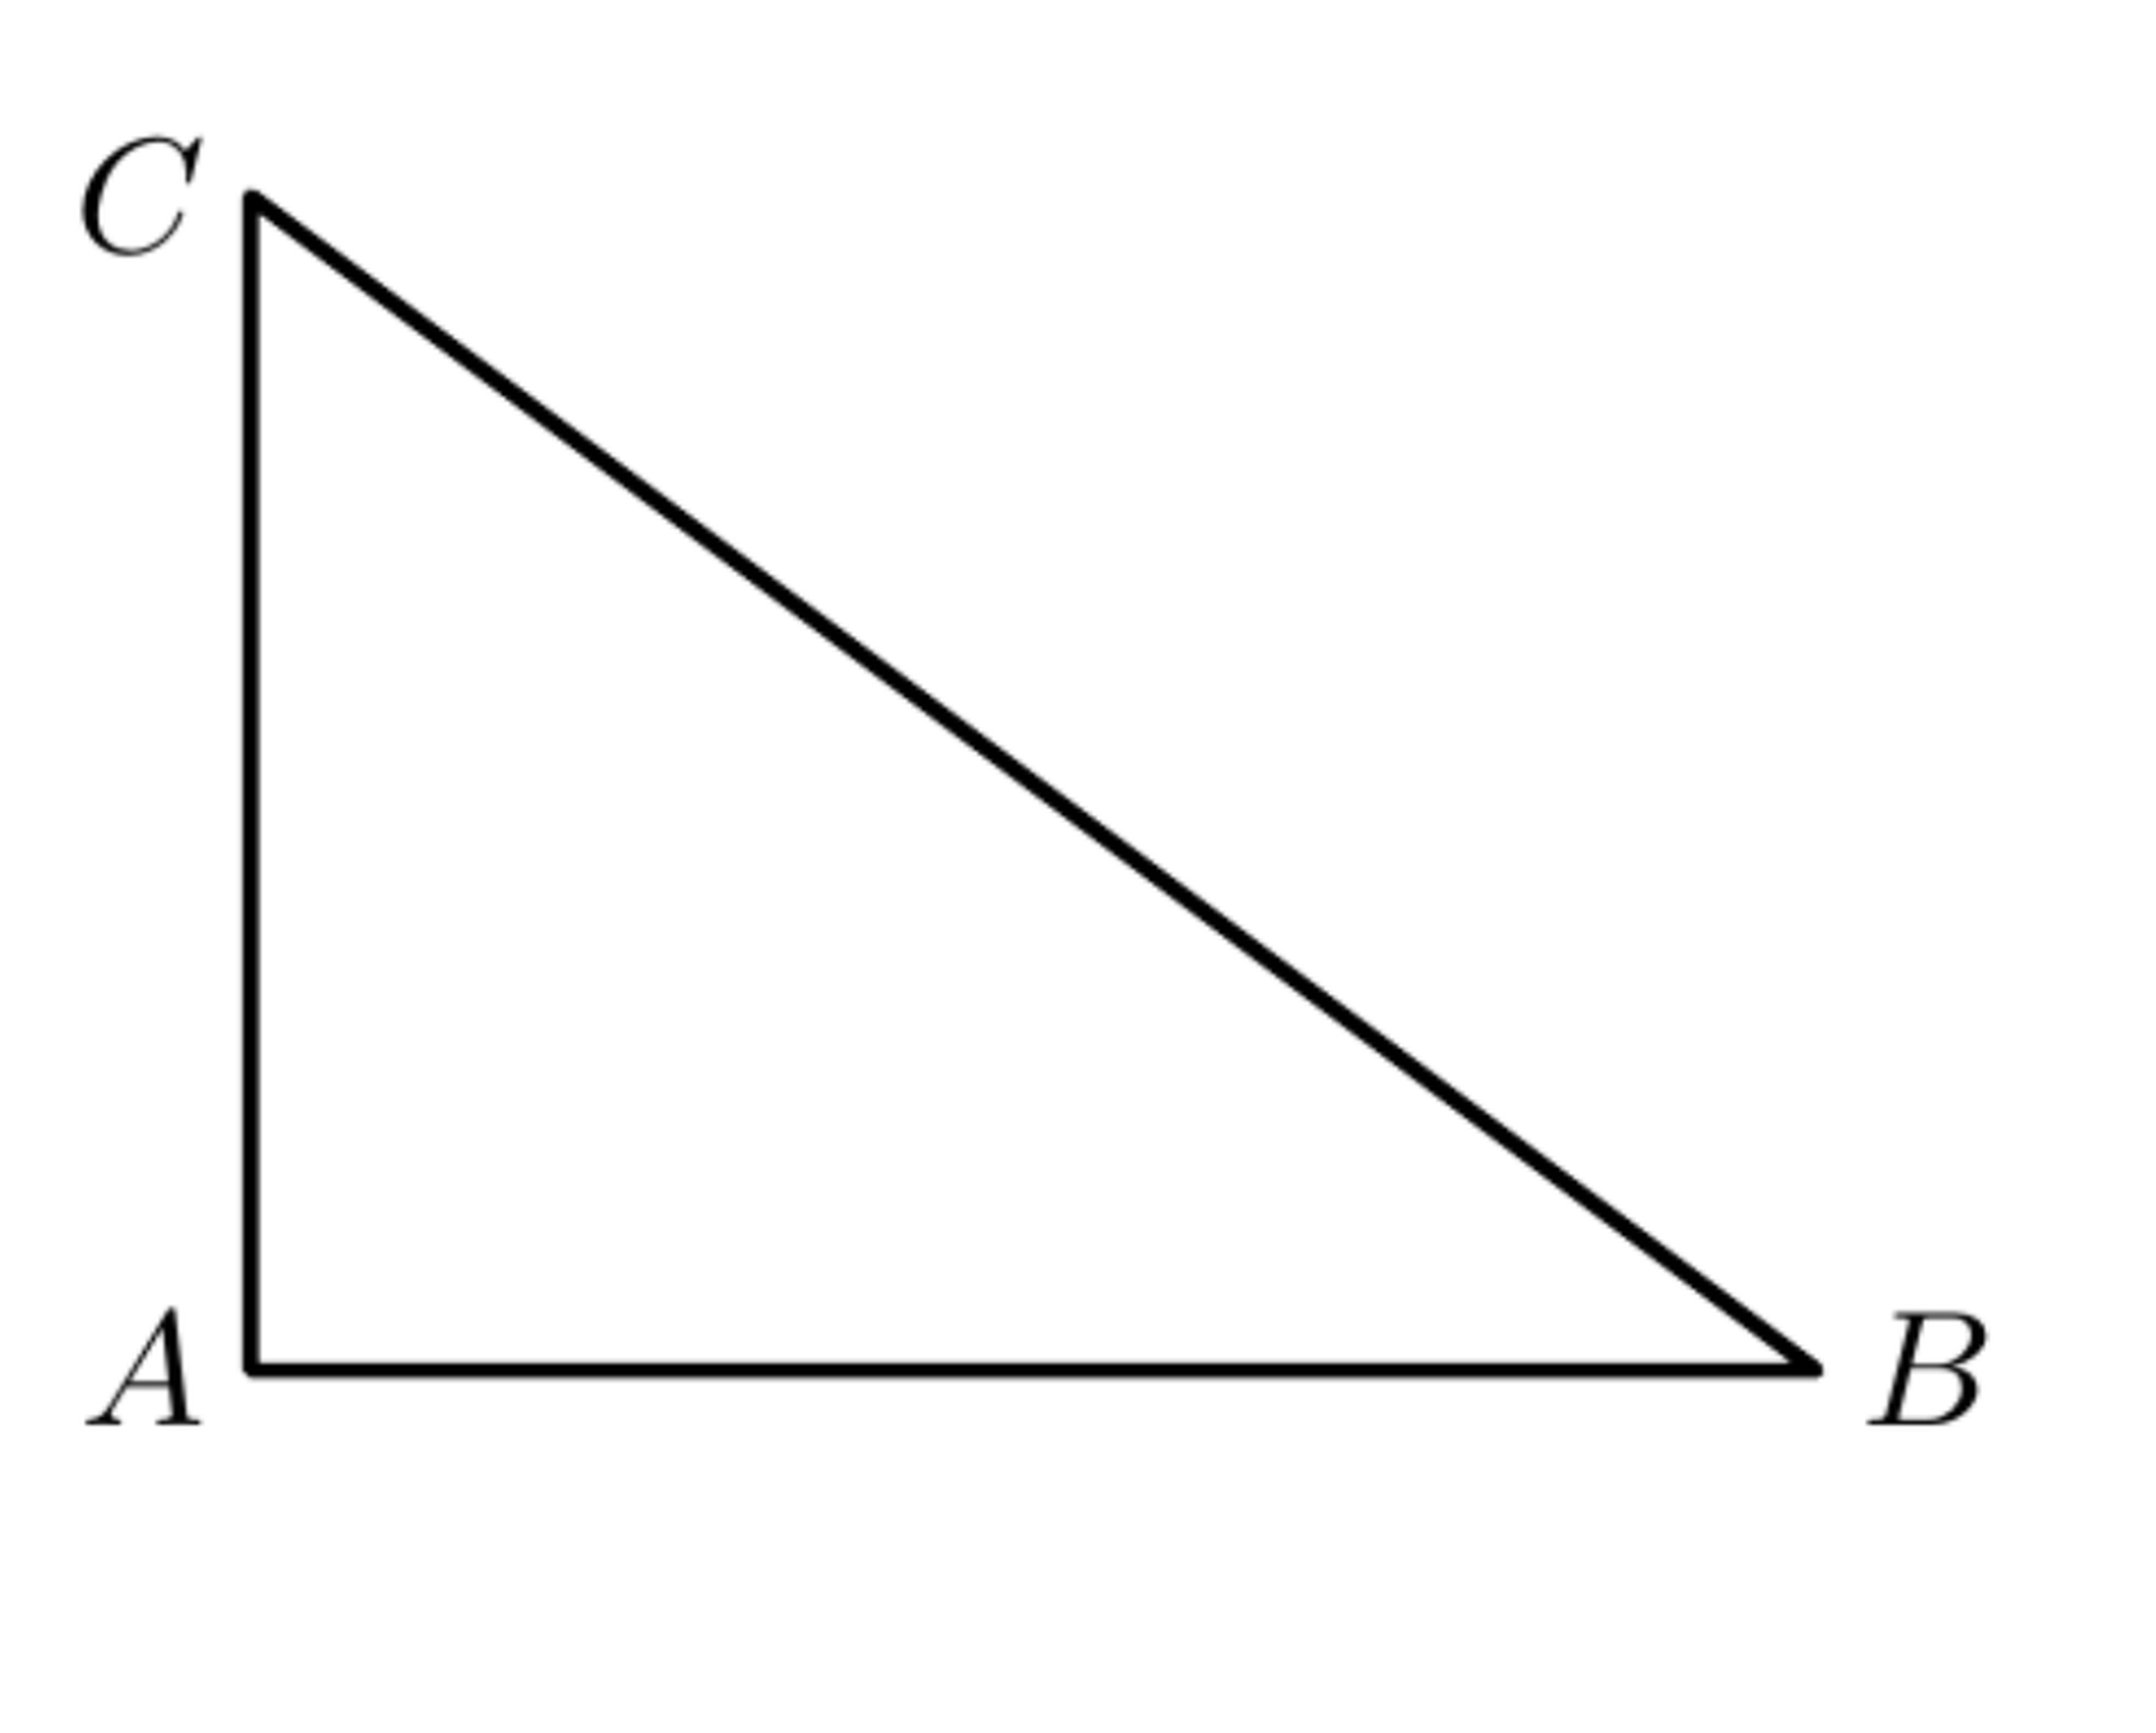
\includegraphics[width=0.34\textwidth]{figures/gao153_q19.png}
\end{center}

\ifanswer
\solbegin
\step{(1) 取 $A(0,0)$、$B(40,0)$、$C(0,30)$，则斜边 $BC$ 所在直线为 $3x+4y=120$.}
\step{正方形落在边界上的两边必分别在两条直角边上.}
\step{设其边长为 $a$m，则对角顶点为 $(a,a)$.}
\step{按题意划出的正方形应尽量大，即对角顶点落在斜边 $BC$ 上，}
\step{因此 $3a+4a=120\Rightarrow a=\dfrac{120}{7}$；}
\step{(2) 斜边长 $BC=\sqrt{30^2+40^2}=50$m，三角形面积为 $600\text{m}^2$.}
\step{设圆的半径为 $r$，圆心到 $AB$、$AC$、$BC$ 的距离分别为 $d_1,d_2,d_3$，}
\step{则三者均不小于 $r$. 连接圆心与三个顶点，}
\step{得 $600=\dfrac12(40d_1+30d_2+50d_3)\geqslant\dfrac12(40+30+50)r=60r$，所以 $r\leqslant10$.}
\step{取三角形的内切圆时等号成立，圆形区域面积的最大值为 $100\pi\text{m}^2$.}
\step{(3) 任取矩形落在绿地边界上的一边，以其所在直线为横轴.}
\step{设相应三角形底边长为 $L$、高为 $H$，则 $LH=1200$.}
\step{取三角形顶点坐标为 $(0,0)$、$(L,0)$、$(p,H)$.}
\step{在高度 $t$ 处，两腰上的点的横坐标分别为 $\dfrac{pt}{H}$、$L+\dfrac{(p-L)t}{H}$，}
\step{因此，高为 $t$ 的矩形，其底边长不超过 $L\left(1-\dfrac tH\right)$，}
\step{面积满足 $S\leqslant Lt\left(1-\dfrac tH\right)=\dfrac LH\left[\dfrac{H^2}{4}-\left(t-\dfrac H2\right)^2\right]\leqslant\dfrac{LH}{4}=300$，}
\step{在原坐标系中，取矩形顶点为 $(0,0)$、$(20,0)$、$(20,15)$、$(0,15)$，}
\step{其中 $3\times20+4\times15=120$，矩形完全位于绿地内，面积为 $300\text{m}^2$，}
\step{达到最大值.}
\solend
\fi

% === Q20 === $g(x)$ 定义照录；解析 14 行
\item 已知 $a>0$ 且 $a\ne1$，设 $f(x)=\log_a(x^2-a^2)$，$g(x)=2\log_a(x-ak)$.

(1) 求函数 $y=f(x)$ 的定义域；

(2) 若 $k=2$，求不等式 $f(x)>g(x)$ 的解集；

(3) 若“存在实数 $x$，使得 $f(x)=g(x)$”为真命题，求实数 $k$ 的取值范围.

\ifanswer
\solbegin
\step{(1) $x^2-a^2>0\Leftrightarrow x<-a$ 或 $x>a$，定义域为 $(-\infty,-a)\cup(a,+\infty)$.}
\step{(2) 两函数均有意义时，$x>2a$，且 $g(x)=\log_a(x-2a)^2$.}
\step{当 $a>1$ 时，$f(x)>g(x)\Leftrightarrow x^2-a^2>(x-2a)^2\Leftrightarrow x>\dfrac{5a}{4}$，}
\step{结合 $x>2a$，解集为 $(2a,+\infty)$.}
\step{当 $0<a<1$ 时，$f(x)>g(x)\Leftrightarrow x^2-a^2<(x-2a)^2\Leftrightarrow x<\dfrac{5a}{4}$，}
\step{与 $x>2a$ 矛盾，解集为 $\varnothing$.}
\step{(3) 在 $x^2-a^2>0$ 且 $x-ak>0$ 的条件下，}
\step{$f(x)=g(x)\Leftrightarrow x^2-a^2=(x-ak)^2\Leftrightarrow2akx=a^2(1+k^2)$，}
\step{当 $k=0$ 时，上式不成立；}
\step{当 $k\ne0$ 时，$x=\dfrac{a(1+k^2)}{2k}$，}
\step{于是 $x-ak=\dfrac{a(1-k^2)}{2k}>0\Leftrightarrow k<-1$ 或 $0<k<1$，}
\step{对上述 $k$，所取的 $x$ 同时满足 $x^2-a^2=(x-ak)^2>0$，}
\step{两函数均有意义且函数值相等.}
\step{因此，$k$ 的取值范围为 $(-\infty,-1)\cup(0,1)$.}
\solend
\fi

% === Q21 === 中文弯引号、复杂式照录；解析 23 行（跨 08→09 页）
\item 若实数 $x$、$y$、$m$ 满足 $\lvert x-m\rvert<\lvert y-m\rvert$，则称 $x$ 比 $y$ 接近 $m$.

(1) 若 $2x$ 比 $x-2$ 更接近 1，求实数 $x$ 的取值范围；

(2) 若 $x$ 比 $y$ 接近 $m$，证明：“$x>y$” 的充要条件是 “$x+y<2m$”；

(3) 已知 $x>0$，$y>0$ 且 $x\ne y$. 设 $p=\dfrac{x^2+y^2}{xy}$，若对于任意的 $x$、$y$，命题 “$p$ 比 $p^2-3p+4$ 接近 $m$” 恒成立，求实数 $m$ 的取值范围.

\ifanswer
\solbegin
\step{(1) $\lvert2x-1\rvert<\lvert x-3\rvert\Leftrightarrow(2x-1)^2<(x-3)^2\Leftrightarrow(x+2)(3x-4)<0$，}
\step{解得 $-2<x<\dfrac43$，实数 $x$ 的取值范围为 $\left(-2,\dfrac43\right)$.}
\step{(2) 因为 $x$ 比 $y$ 接近 $m$，所以 $\lvert x-m\rvert<\lvert y-m\rvert$，则 $\lvert x-m\rvert^2<\lvert y-m\rvert^2$，}
\step{即 $(x-m)^2<(y-m)^2$，即 $(x-m)^2-(y-m)^2<0$，}
\step{即得 $(x-y)(x+y-2m)<0$，}
\step{则由 $x+y<2m$，得 $x+y-2m<0$，}
\step{故 $x-y>0$，即 $x>y$，充分性成立；}
\step{当 $x>y$ 时，$x-y>0$，结合 $(x-y)(x+y-2m)<0$，得 $x+y-2m<0$，}
\step{即 $x+y<2m$，必要性成立；}
\step{故“$x>y$” 的充要条件是 “$x+y<2m$”；}
\step{(3) $x>0$，$y>0$ 且 $x\ne y$. 则 $p=\dfrac{x^2+y^2}{xy}=\dfrac xy+\dfrac yx>2\sqrt{\dfrac xy\cdot\dfrac yx}=2$，}
\step{由于对于任意的 $x$、$y$，命题 “$p$ 比 $p^2-3p+4$ 接近 $m$” 恒成立，}
\step{故 $\lvert p-m\rvert<\lvert(p^2-3p+4)-m\rvert$ 对 $\forall p>2$ 恒成立，}
\step{即得 $(p-m)^2<(p^2-3p+4-m)^2$，}
\step{即 $(p^2-3p+4-m)^2-(p-m)^2>0$，}
\step{得 $(p^2-4p+4)(p^2-2p+4-2m)>0$，}
\step{即 $(p-2)^2(p^2-2p+4-2m)>0$，由于 $p>2$，故 $(p-2)^2>0$，}
\step{故 $p^2-2p+4-2m>0$ 对 $\forall p>2$ 恒成立，}
\step{即 $2m<p^2-2p+4$ 对 $\forall p>2$ 恒成立，}
\step{由于 $p^2-2p+4=(p-1)^2+3$，此时 $p^2-2p+4$ 在 $(2,+\infty)$ 上严格增，}
\step{故 $(p-1)^2+3>(2-1)^2+3=4$，故 $2m\leqslant4$，解得 $m\leqslant2$，}
\step{即实数 $m$ 的取值范围是 $(-\infty,2]$.}
\solend
\fi

\end{enumerate}

\end{document}
"
%
% ① 原始材料：微信公众号"魔都数学加油站"文章，连载"27学年高一153"，原文标题
% "27学年高一153——2026-2027年上海市闵行中学文绮中学高一上期中"；
% 原文链接：https://mp.weixin.qq.com/s/rEtS-92cDR6JKgY2b5DRfg 。
% 正文为 9 张 PNG 页（01/02/06/07/08/09 为 2560×3620，03/04/05 为 4762×6735，
% 同一篇各页分辨率混排，逐页按各自分辨率裁图核对，别按预览比例换算裁框）。
% 体例：讲评版——填空 3—12（10 题）、选择 13—16（4 题）、解答 17—21（5 题），
% 共 19 题，自第 3 题起编；**全 19 题均印【解析】**（逐题核实，见 ② ②）。
% 题目、答案、解析均据原图转录；卷面粉红色水印"魔都数学加油站"及公众号页脚未录入。
% 全卷插图清单（逐页通读 9 页确认）：2 幅，均为题目配图、三版都出——
%   · Q11 正方形 OABC 曲线图（02 页右下：$y=5x^2$ 与 $y=x^{-\frac12}$ 两条曲线、
%     坐标轴、O/A/B/C/P/Q、正方形），裁 figures/gao153_q11.png；
%   · Q19 直角三角形 ABC 绿地示意图（05 页右上，直角在 A），
%     裁 figures/gao153_q19.png；
%   两图均去粉色水印、去色、4× LANCZOS 放大；Q11 图左上角题干残字"函"已裁白。
%   其余各页逐页确认无其它题目配图、无解析内配图、无表格；09 页下半仅水印、无正文。
%
% 卷首标题：原卷印作"2026-2027 年闵行中学文绮中学高一上期中"，年份区间按全稿惯例排 en dash；
% 原卷卷面未印副标题，本稿按同期中卷知识模块口径补出"集合与常用逻辑用语、不等式、函数"。
%
% ② 与原卷的排版差异：
%   ① 原文从第 3 题起，本稿保留原题号；共 19 题三节，解答题 5 题到 21；
%   ② 全 19 题均印【解析】、用 \solbegin…\solend，无只印【答案】或答案印括号内的题；
%      四道选择题答案在解析末句"故选 A／A／D／C"（Q13—Q16，逐个放大复核）、
%      括号 \mbox{（\quad）} 留空、不另提 \ans{}；答案版【答案】/【解析】标记数
%      = 19 = 全卷题数；
%   ③ 原卷卷面未印副标题，本稿按知识模块口径补出；
%   ④ 原卷填空横线按全稿惯例排 \blankline[4.4em]；选择题括号排 \mbox{（\quad）}、
%      四道选择题的选项段前按惯例各加 \keepwithprev；解答题不留作答区、不加
%      \anspace（原卷为讲评版，109—113 起全稿不用 \anspace）；
%   ⑤ 数集：Q3"$x\in R$"、Q5"解集为 R"、Q10"$x\in N$"、Q12"$x\in Z$"与
%      "$m\in Z$"、Q14"$m\in Z$"、Q16"$a\in N$"、Q17"全集 $U=R$"、
%      Q19 无、Q21 无——原卷印斜体或正体粗体 R/N/Z，按全稿惯例归一
%      \R／\N／\Z；绝对值排 \lvert…\rvert（Q5、Q11、Q21），集合描述竖线排 \mid
%      （Q3、Q10、Q17、Q20），不等号按全稿惯例排 \leqslant／\geqslant；
%      补集照原卷上划线排 \overline{A}（Q17 题干 (2)＋解析 (2)）；
%      空集 \varnothing（Q12 题干、Q20 解析 (2)）；子集 3 处均印带下划线 ⊆、
%      照录 \subseteq（Q10 $A\subseteq U$、Q12 $B\subseteq A$、Q17 $(-1,2)\subseteq(a-5,a)$），
%      本卷无单线 \subset 用例；
%   ⑥ 判别式：逐页通读 9 页，本卷无一元二次判别式 Δ/△ 算式，故无 Δ/△ 混用可照录；
%      Q11 图里有几何正方形 OABC（非三角形符号），无 △ABC 用例；
%   ⑦ 中文弯引号照录：Q14"$m=0$"与"幂函数…关于原点成中心对称"、
%      Q20"存在实数 $x$，使得 $f(x)=g(x)$"、Q21"$x>y$"与"$x+y<2m$"、
%      "$p$ 比 $p^2-3p+4$ 接近 $m$"（引号外留空格按原卷）；
%      注释里一律 ASCII 引号；数学式内 CJK 用 \text{}；
%   ⑧ "图像／图象"逐处放大核：全卷 3 处均印"图像"（像，有亻）——
%      Q13 题干与解析、Q14 题干与解析；Q19 题干写"如图所示"（非"图像"），
%      逐处照录未统一；子题标号 (1)(2)(3) 半角括号照录；圈数字本卷无用例；
%   ⑨ 半角逗号在数学组之间是全稿惯例、非笔误，逐处照录（Q3 $x\in R$、
%      Q10 $a_1,a_2$、Q19 $A(0,0)$、$d_1,d_2,d_3$、Q21 $a>\frac13,b>\frac13$ 等）；
%      行末西文句点 ASCII `.`；行中全角逗号／顿号照录（Q19"30m 和 40m"、
%      Q21"实数 $x$、$y$、$m$"）；
%   ⑩ 复杂式照录别简化：Q3 $y=x^{-2}$、Q11 $y=x^{-\frac12}$ 与
%      $\frac{2}{\sqrt[4]{5}}$、Q8 $\frac{2b}{a+1-b}$、Q9 cases 块、
%      Q10 $525=5\times105$、Q16 $a^2+1$、Q19 $S\leqslant Lt(1-\frac tH)$
%      与 $L+\frac{(p-L)t}{H}$、Q20 $2akx=a^2(1+k^2)$ 与 $\frac{a(1+k^2)}{2k}$、
%      Q21 $(p^2-4p+4)(p^2-2p+4-2m)>0$；
%      \left…\right 不得拆到不同 $…$ 组（Q17 $\left\{x\mid\cdots\right\}$、
%      Q19 $\left[\frac{H^2}{4}-\left(t-\frac H2\right)^2\right]$、
%      Q21 $\left(-2,\frac43\right)$ 等）；cases 块一律 \begin{cases}…\end{cases}；
%   ⑪ 一条 \step = 原卷解析的一个印刷行，cases 块整体算一个印刷行；别并折行、
%      别拆行。Q10 六行、Q19 十九行、Q20 十四行、Q21 二十二行均按印刷行逐条断，
%      不丢行；
%   ⑫ 配图：Q11／Q19 题目配图（三版都出）放 \item 内题干之后 \begin{center}，
%      各用 \needvspace{8cm} 守卫把整块推走，**守卫放在 \item 之前**
%      （见 高一145 Q14/Q20 成例与切页审计 B 类坑）；
%   ⑬ 原卷解析内无红色"法一／法二"之类小标题，故本卷无 \stepm；红色水印
%      "魔都数学加油站"不录入；
%   ⑭ 跨页续印按题合并：见 ⑥；
%
% ③ 行数复核：一条 \step = 原卷解析的一个印刷行，cases 块作一个印刷行计。
%   逐题数（主会话逐页核对定稿）：Q3：1；Q4：2；Q5：2；Q6：2；Q7：1；
%   Q8：1；Q9：2；Q10：6；Q11：3；Q12：5；Q13：2；Q14：3；Q15：5；
%   Q16：3；Q17：5；Q18：4；Q19：19；Q20：14；Q21：22。
%   合计 102 条 \step（本卷无 \stepm），与原卷逐题印刷行相等。全卷 19 题
%   均设 \solbegin…\solend，答案版【答案】/【解析】标记数 = 19 = 全卷题数。
%
% ④ 判别式／子集符号结论（逐处放大原图照录、不得统一，主会话像素级复核）：
%   判别式：逐页通读 9 页，本卷无一元二次判别式算式（Q7 用韦达定理、
%      Q16 用因式分解、Q20 用对数方程，均不写 Δ/△），故无 Δ/△ 混用可照录
%      （"高 \Delta／扁 \triangle"口径备查，参照 高一142／151／152 头注）；
%      本卷无几何三角形符号用例。
%   子集：Q10 题干"$A\subseteq U$"、Q12 题干"$B\subseteq A$"、Q17 解析 (2)
%      "$(-1,2)\subseteq(a-5,a)$"共 3 处，逐处放大确认均印带下划线 ⊆、
%      照录 \subseteq；本卷未见单线 ⊂（\subset）之对应处。
%      补集上划线 \overline{A}（Q17）、空集 \varnothing（Q12 题干、Q20 解析 (2)）；
%      数集 \R／\N／\Z 归一见 ② ⑤。
%
% ⑤ 存疑照录（放大原图确认，照录未改、正文对应处另有 % 注）：
%   1. Q3 集合 $B=\{(x,y)\mid y=x^{-2},x\in\R\}$ 原卷题干径写 $x\in\R$
%      （$x=0$ 处无意义），解析自行注明 $x\ne0$，照录未改。
%   2. Q10 解析"$U$ 中共有 $525=5\times105$ 个连续整数"与尾行
%      "取 $U$ 中除以 5 余 1 或 2 的全部元素及元素 5"逐字照录（放大 02 页
%      /tmp/gao153/z/zoom/q10_pick.png 确认是"元素 5"，非"元素 9"）。
%   3. Q11 第二个函数原卷印 $y=x^{-\frac12}$（负二分之一次幂，非 $x^2$），
%      放大 02 页 /tmp/gao153/z/zoom/q11_exp.png 确认，照录未改；
%      $|AQ|=\frac1{\sqrt a}$ 与之自洽。
%   4. Q19 (3) 解析"在高度 $t$ 处，两腰上的点的横坐标分别为 $\frac{pt}{H}$、
%      $L+\frac{(p-L)t}{H}$"，放大 06 页确认，照录未简化。
%   5. Q20 (2) 解析"$g(x)=\log_a(x-2a)^2$"（真数整体平方），
%      与 $g(x)=2\log_a(x-ak)$ 在 $k=2$ 时一致，照录未改。
%   6. Q21 (3) 解析"得 $(p^2-4p+4)(p^2-2p+4-2m)>0$"与
%      "故 $(p-1)^2+3>(2-1)^2+3=4$，故 $2m\leqslant4$"照录未改
%      （放大 09 页 /tmp/gao153/z/zoom/q21_factor.png 确认）。
%   7. "图像／图象"全卷 3 处均印"图像"（像，有亻）逐处照录；
%      本卷无判别式 Δ/△ 用例（见 ④）。
%   全卷除此 7 类外未发现其它笔误／自相矛盾处；19 题均印【解析】、
%   无只印【答案】或答案印括号内的题（见 ② ②）。
%
% ⑥ 跨页续印按题合并说明（逐页核实定稿）：Q3—Q5 题干＋解析在 01 页；
%   Q6—Q8 题干＋解析在 01 页下半（Q8 解析续 02 页顶）；Q9 题干＋解析、
%   Q10 题干＋解析首 2 行在 02 页上半，Q10 解析余 4 行在 02 页下半；
%   Q11 题干＋配图＋解析、Q12 题干＋解析 5 行在 02 页下半—03 页上半；
%   "二、选择题"标题在 03 页中部；Q13 题干＋选项＋解析在 03 页下半；
%   Q14 题干＋选项＋解析、Q15 题干＋选项＋解析首行在 03 页下半—04 页顶；
%   Q15 解析余 4 行、Q16 题干＋选项＋解析在 04 页上半；"三、解答题"
%   标题在 04 页下半；Q17 题干＋两问＋解析 5 行在 04 页下半—05 页顶；
%   Q18 题干＋两问＋解析 4 行、Q19 题干（含配图）＋三问在 05 页；
%   Q19 解析 (1)(2) 9 行在 05 页下半，解析 (3) 前 5 行在 06 页上半、
%   余 4 行在 06 页下半；Q20 题干＋三问在 06 页下半，解析 (1)(2)(3)
%   前 6 行在 07 页上半、(3) 余 8 行在 07 页下半；Q21 题干＋三问在
%   07 页末，解析 (1)(2) 10 行在 08 页上半—下半，解析 (3) 前 4 行在
%   08 页下半、余 9 行续 09 页上半，末行"即实数 $m$ 的取值范围是
%   $(-\infty,2]$"为全卷收尾（09 页下半仅水印、无正文）。
%   本稿按题连排，不丢行、不并折行；全卷末题为第 21 题，无附加题节。
%
\documentclass[a4paper,11pt]{article}
\usepackage{common}

\begin{document}

\examtitlest[3]{2026--2027 年闵行中学文绮中学高一上期中}{集合与常用逻辑用语、不等式、函数}

\bigsec{一、填空题}

\begin{enumerate}
\setcounter{enumi}{2}

% === Q3 === 集合描述竖线 \mid；$y=x^{-2}$ 照录；解析 1 行
\item 已知 $A=\{(x,y)\mid y=x^3,x\in\R\}$，$B=\{(x,y)\mid y=x^{-2},x\in\R\}$，则 $A\cap B=$\blankline[4.4em].

\ifanswer
\solbegin
\step{$x^3=x^{-2}\ (x\ne0)\Leftrightarrow x^5=1\Leftrightarrow x=1$，此时 $y=1$，所以 $A\cap B=\{(1,1)\}$.}
\solend
\fi

% === Q4 === 解析 2 行
\item 若关于 $x$ 的不等式 $\dfrac{x-a}{x+1}>0$ 的解集为 $(-\infty,-1)\cup(4,+\infty)$，则实数 $a=$\blankline[4.4em].

\ifanswer
\solbegin
\step{关于 $x$ 的不等式 $\dfrac{x-a}{x+1}>0$ 即 $(x+1)(x-a)>0$.}
\step{再由它的解集为 $(-\infty,-1)\cup(4,+\infty)$，得 $-1$ 和 4 是 $(x+1)(x-a)=0$ 的两个实数根，故 $a=4$.}
\solend
\fi

% === Q5 === 绝对值 \lvert…\rvert；解析 2 行
\item 若关于 $x$ 的不等式 $\lvert x+1\rvert+\lvert x-2\rvert>m$ 的解集为 $\R$，则实数 $m$ 的取值范围是\blankline[4.4em].

\ifanswer
\solbegin
\step{$\lvert x+1\rvert+\lvert x-2\rvert\geqslant\lvert(x+1)-(x-2)\rvert=3$，当且仅当 $-1\leqslant x\leqslant2$ 时取等号，}
\step{因此 $m<3$.}
\solend
\fi

% === Q6 === 解析 2 行
\item 已知指数函数 $y=a^x$（$a>1$）在区间 $[-1,1]$ 上的最大值比最小值大 $\dfrac32$，则实数 $a=$\blankline[4.4em].

\ifanswer
\solbegin
\step{$a>1$，指数函数在 $[-1,1]$ 上严格增，故 $a-\dfrac1a=\dfrac32\Leftrightarrow(a-2)(2a+1)=0$.}
\step{结合 $a>1$，得 $a=2$.}
\solend
\fi

% === Q7 === 韦达定理；解析 1 行
\item 已知关于 $x$ 的一元二次方程 $x^2+px+2p=0$ 的两个实数根分别为 $x_1$、$x_2$，且 $(x_1+1)(x_2+1)=0$，则 $p=$\blankline[4.4em].

\ifanswer
\solbegin
\step{$0=(x_1+1)(x_2+1)=x_1x_2+x_1+x_2+1=2p-p+1=p+1\Rightarrow p=-1$.}
\solend
\fi

% === Q8 === 换底公式；解析 1 行
\item 已知 $10^a=3$，$\lg5=b$，则 $\log_6 25=$\blankline[4.4em]（用关于 $a,b$ 的关系式表示）.

\ifanswer
\solbegin
\step{$\lg3=a$，$\lg2=1-b$，所以 $\log_6 25=\dfrac{\lg25}{\lg6}=\dfrac{2b}{a+1-b}$.}
\solend
\fi

% === Q9 === cases 块整体算一个印刷行；解析 2 行
\item 已知 $A=[2,5]$，若对任意 $x\in A$，总有 $\dfrac{k}{x}\in A$，则正数 $k=$\blankline[4.4em].

\ifanswer
\solbegin
\step{$k>0$，当 $x\in[2,5]$ 时，$\dfrac{k}{x}$ 的取值范围为 $\left[\dfrac k5,\dfrac k2\right]$，}
\step{因此 $\begin{cases}\dfrac k5\geqslant2\\\dfrac k2\leqslant5\end{cases}\Leftrightarrow10\leqslant k\leqslant10\Leftrightarrow k=10$.}
\solend
\fi

% === Q10 === $A\subseteq U$ 带下划线照录；解析 6 行
\item 已知集合 $U=\{x\mid4\leqslant x\leqslant528,x\in\N\}$，$A=\{a_1,a_2,a_3,\cdots,a_n\}$，且 $A\subseteq U$. 如果集合 $A$ 中的任意两个不同元素之和都不能被 5 整除，则正整数 $n$ 的最大值为\blankline[4.4em].

\ifanswer
\solbegin
\step{$U$ 中共有 $525=5\times105$ 个连续整数，按除以 5 的余数分成五类，}
\step{每类均有 105 个元素.}
\step{余数为 1,4 的两类不能同时选取，余数为 2,3 的两类也不能同时选取，}
\step{余数为 0 的一类最多选 1 个，因此 $n\leqslant105+105+1=211$.}
\step{取 $U$ 中除以 5 余 1 或 2 的全部元素及元素 5，}% 放大 02 页确认是「元素 5」（非 9），照录未改（见 ⑤ 2）
\step{任意两个不同元素之和均不能被 5 整除，此时 $n=211$，最大值为 211.}
\solend
\fi

% === Q11 === 题目配图（三版都出）；\needvspace 守卫放 \item 之前；$y=x^{-\frac12}$ 照录；解析 3 行
\needvspace{8cm}
\item 如图，已知正方形 $OABC$，其中 $OA=a$（$a>1$），函数 $y=5x^2$ 交 $BC$ 于点 $P$，函数 $y=x^{-\frac12}$ 交 $AB$ 于点 $Q$，当 $\lvert AQ\rvert+\lvert CP\rvert$ 最小时，$a$ 的值为\blankline[4.4em].

\begin{center}
% 正方形 OABC 与两条曲线图取 02 页右下，去粉色水印、去色、4× LANCZOS 放大；三版都出
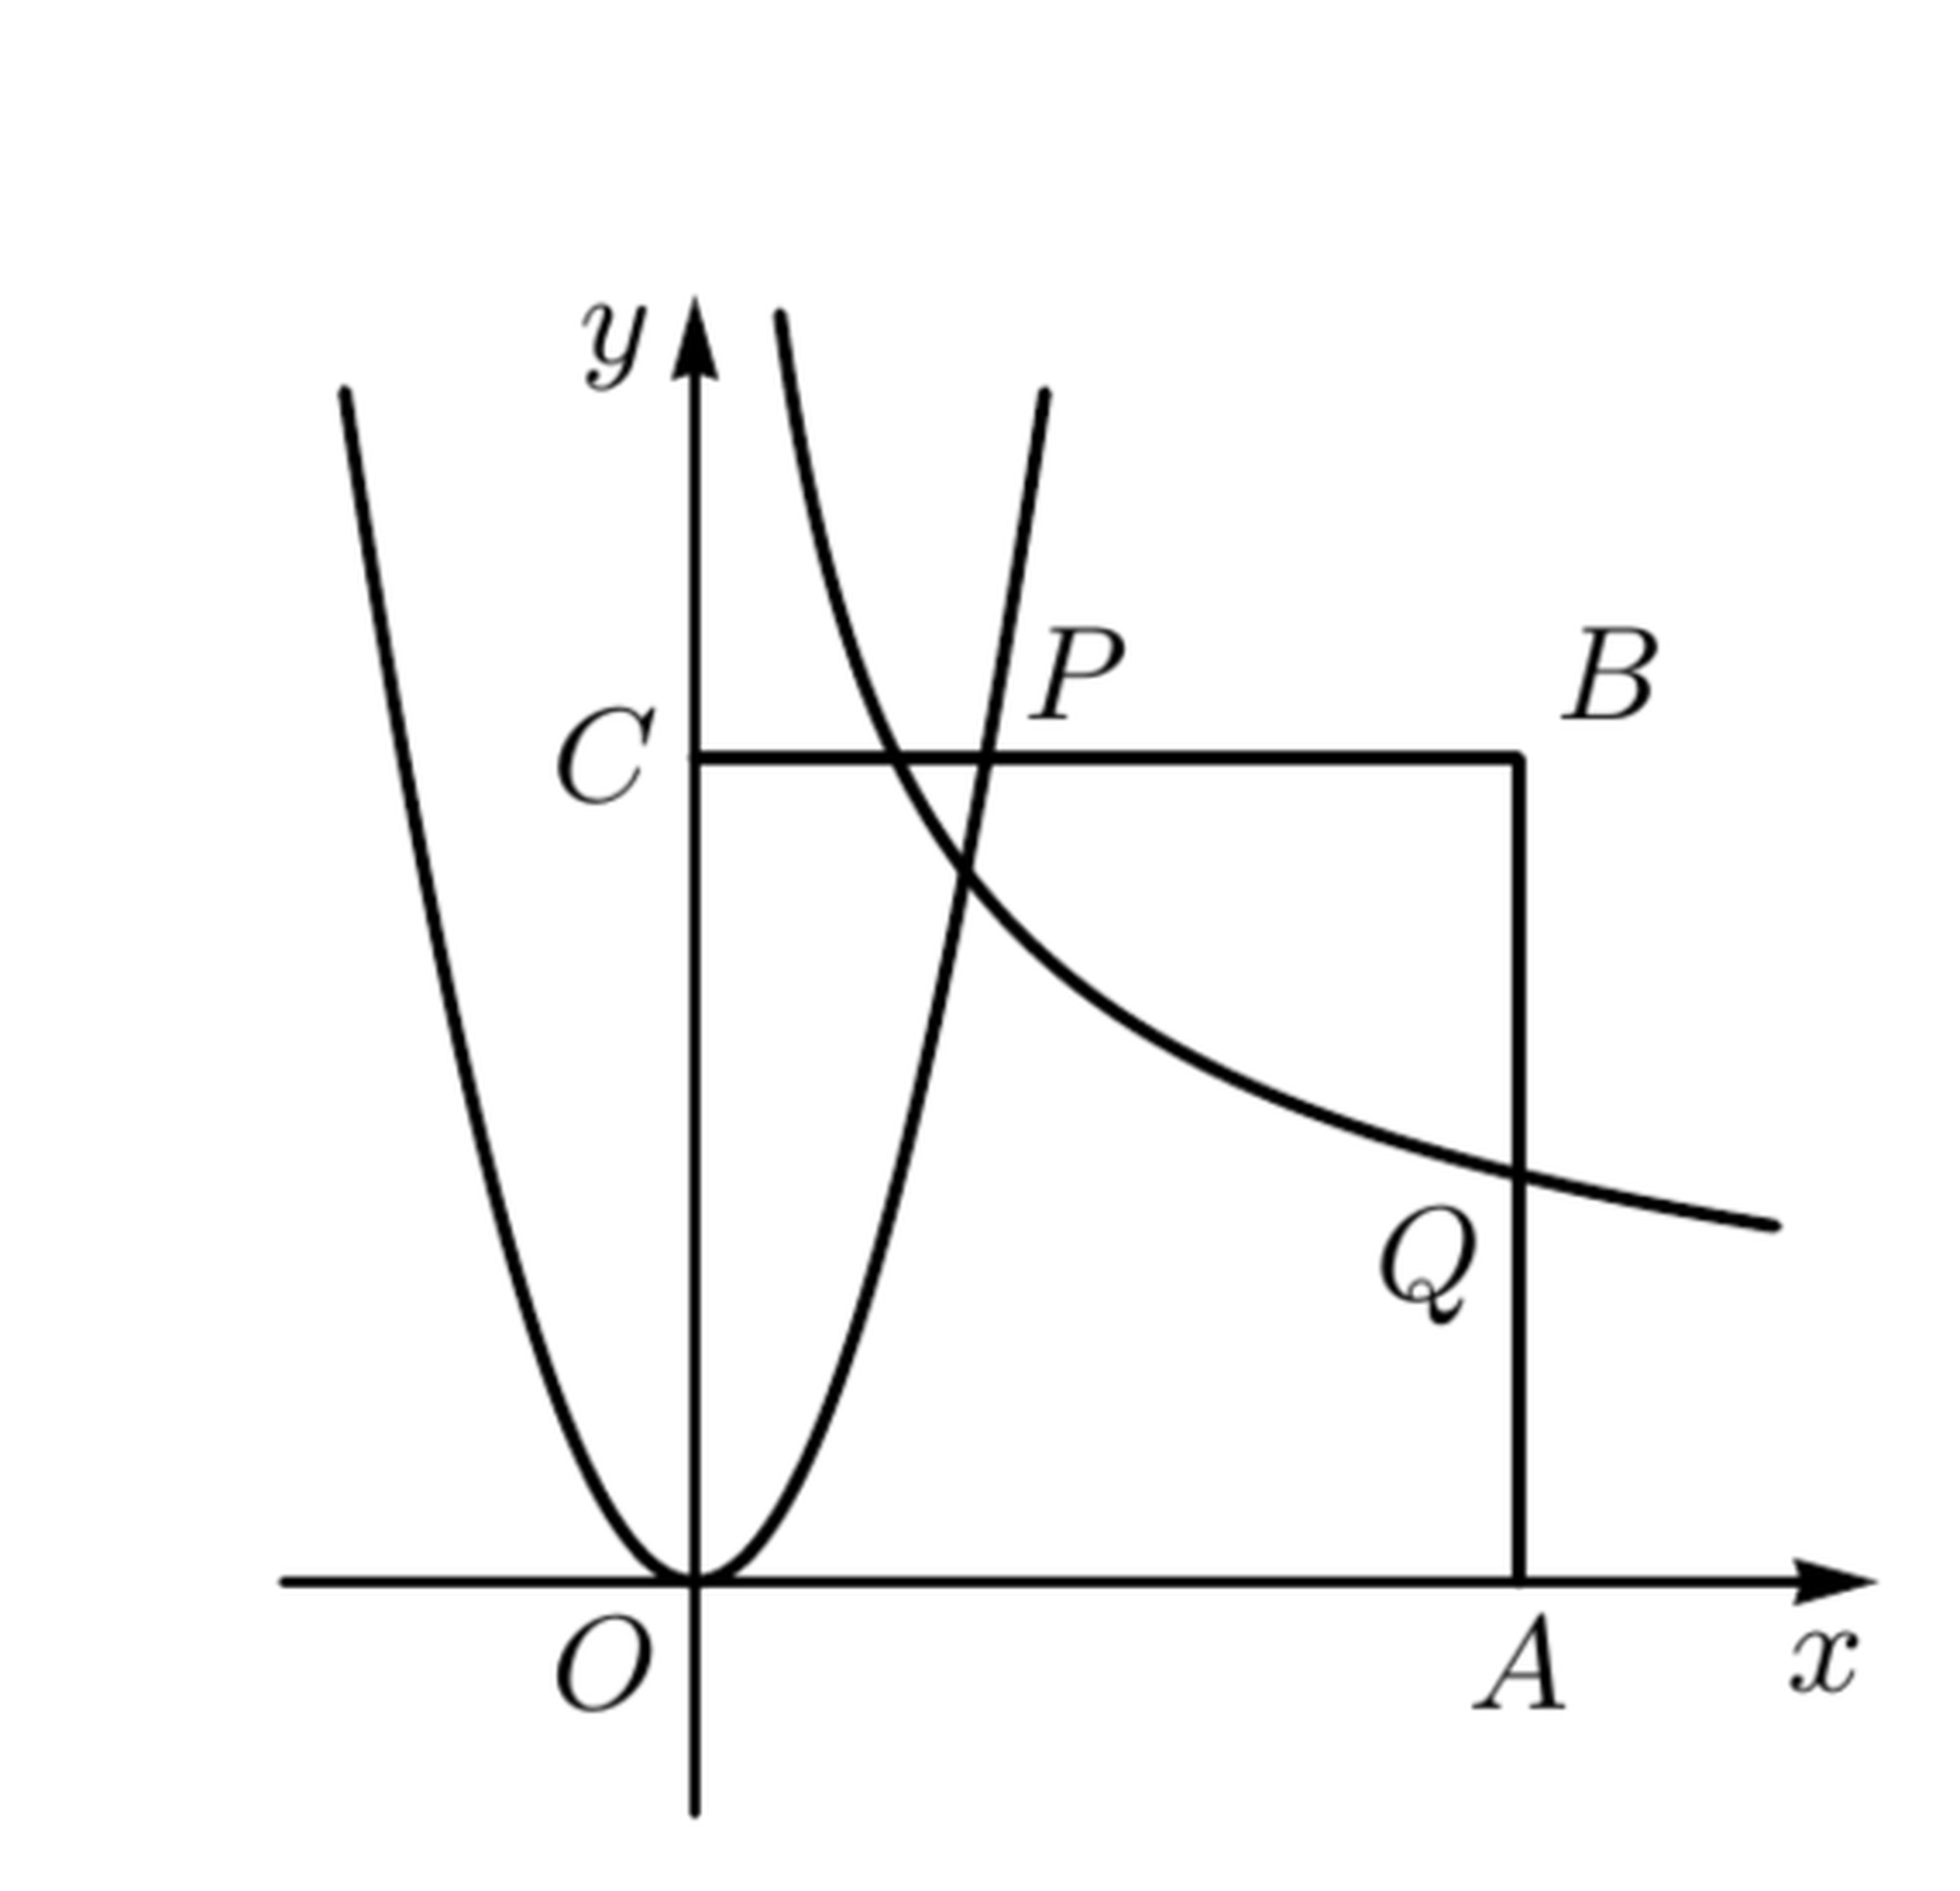
\includegraphics[width=0.40\textwidth]{figures/gao153_q11.png}
\end{center}

\ifanswer
\solbegin
\step{$\lvert AQ\rvert=\dfrac1{\sqrt a}$，$\lvert CP\rvert=\sqrt{\dfrac a5}$，}
\step{于是 $\lvert AQ\rvert+\lvert CP\rvert=\dfrac1{\sqrt a}+\sqrt{\dfrac a5}\geqslant2\sqrt{\dfrac1{\sqrt a}\cdot\sqrt{\dfrac a5}}=\dfrac2{\sqrt[4]{5}}$，}
\step{当且仅当 $\dfrac1{\sqrt a}=\sqrt{\dfrac a5}$，即 $a=\sqrt5$ 时取等号.}
\solend
\fi

% === Q12 === $B\subseteq A$ 带下划线照录、空集 \varnothing；解析 5 行
\item 若集合 $A=\{x\mid1\leqslant x\leqslant100,x\in\Z\}$，集合 $B\subseteq A$，且 $B\ne\varnothing$，记 $W(B)$ 为 $B$ 中元素的最大值与最小值之和，则对所有的 $B$，$W(B)$ 的平均值是\blankline[4.4em].

\ifanswer
\solbegin
\step{对每个非空子集 $B$，令 $B'=\{101-x\mid x\in B\}$，}
\step{则 $W(B')=(101-\min B)+(101-\max B)=202-W(B)$.}
\step{对 $B'$ 再作同样变换即得到 $B$，因此 $B$ 遍历所有非空子集时，}
\step{$B'$ 也恰好遍历所有非空子集.}
\step{设所求平均值为 $m$，则 $m=202-m$，解得 $m=101$.}
\solend
\fi

\end{enumerate}

\bigsec{二、选择题}

\begin{enumerate}
\setcounter{enumi}{12}

% === Q13 === "图像"（像，有亻）照录；解析 2 行，故选 A
\item 设 $a$、$b$ 为常数，若 $0<a<1$，$b>1$，则函数 $y=a^x-b$ 的图像必定不经过\mbox{（\quad）}

\keepwithprev
A. 第一象限\qquad\qquad B. 第二象限\qquad\qquad C. 第三象限\qquad\qquad D. 第四象限

\ifanswer
\solbegin
\step{当 $x>0$ 时，$a^x<1<b$，所以 $y=a^x-b<0$，图像必定不经过第一象限，}
\step{故选 $A$.}
\solend
\fi

% === Q14 === $m\in\Z$、中文弯引号、"图像"照录；解析 3 行，故选 A
\item 已知 $m\in\Z$，则“$m=0$”是“幂函数 $y=x^{m^2-2m-1}$ 的图像与 $x$ 轴及 $y$ 轴均无交点，且关于原点成中心对称”的\mbox{（\quad）}

\keepwithprev
A. 充分不必要条件\qquad\qquad B. 必要不充分条件

C. 充要条件\qquad\qquad D. 既不充分也不必要条件

\ifanswer
\solbegin
\step{图像满足所述条件 $\Leftrightarrow m^2-2m-1$ 为负奇数 $\Leftrightarrow m=0$ 或 $m=2$.}
\step{$m=0$ 能推出所述条件，但所述条件不能推出 $m=0$，因此是充分不必要条件，}
\step{故选 $A$.}
\solend
\fi

% === Q15 === 四选项一行；解析 5 行（跨 03→04 页），故选 D
\item 设 $a>b>1$，$x>1$，则下列不等式正确的是\mbox{（\quad）}

\keepwithprev
A. $a^x<b^x$\qquad B. $x^a<x^b$\qquad C. $\log_a x>\log_b x$\qquad D. $\log_x a>\log_x b$

\ifanswer
\solbegin
\step{$x>1$，幂函数与指数函数的单调性给出 $a^x>b^x$，$x^a>x^b$，A、B 错误.}
\step{$\log_a x=\dfrac{\lg x}{\lg a}<\dfrac{\lg x}{\lg b}=\log_b x$，C 错误.}
\step{对数函数 $y=\log_x t$ 的底数 $x>1$，在 $(0,+\infty)$ 上严格递增，}
\step{所以 $\log_x a>\log_x b$，D 正确.}
\step{故选 $D$.}
\solend
\fi

% === Q16 === $a\in\N$；解析 3 行，故选 C
\item 设 $a\in\N$，则满足不等式 $x^2-a^2x-a^2-1<0$ 的整数 $x$ 的个数不可能是\mbox{（\quad）}

\keepwithprev
A. 1\qquad\qquad B. 50\qquad\qquad C. 100\qquad\qquad D. 2026

\ifanswer
\solbegin
\step{$(x+1)(x-a^2-1)<0\Leftrightarrow-1<x<a^2+1$. 整数解为 $0,1,\cdots,a^2$，共 $a^2+1$ 个.}
\step{$1=0^2+1$，$50=7^2+1$，$2026=45^2+1$，而 $100-1=99$ 不是完全平方数，}
\step{故选 $C$.}
\solend
\fi

\end{enumerate}

\bigsec{三、解答题}

\begin{enumerate}
\setcounter{enumi}{16}

% === Q17 === 补集上划线 \overline{A}、\subseteq 照录；解析 5 行
\item 已知全集 $U=\R$，集合 $A=\{x\mid x^2-x-2\geqslant0\}$，$B=\{x\mid x>-1\}$，$C=\{x\mid a-5<x<a\}$.

(1) 求 $A\cap B$、$A\cup B$；

(2) 若 $\overline{A}\cup C=C$，求实数 $a$ 的取值范围.

\ifanswer
\solbegin
\step{(1) $x^2-x-2=(x+1)(x-2)\geqslant0\Leftrightarrow x\leqslant-1$ 或 $x\geqslant2$，}
\step{所以 $A=(-\infty,-1]\cup[2,+\infty)$，$B=(-1,+\infty)$，}
\step{因此 $A\cap B=[2,+\infty)$，$A\cup B=\R$.}
\step{(2) $\overline{A}=(-1,2)$，于是 $\overline{A}\cup C=C\Leftrightarrow\overline{A}\subseteq C\Leftrightarrow(-1,2)\subseteq(a-5,a)$，}
\step{两区间均为开区间，端点可重合，故 $\begin{cases}a-5\leqslant-1\\a\geqslant2\end{cases}\Leftrightarrow2\leqslant a\leqslant4$.}
\solend
\fi

% === Q18 === 解析 4 行
\item 已知 $a$、$b$、$c$ 都是正数，

(1) 若 $a+b=1$，求证：$\dfrac1a+\dfrac1b\geqslant4$，并指出等号成立的条件；

(2) 若 $a+b+c=1$，求证：三个数 $\dfrac1a$、$\dfrac1b$、$\dfrac1c$ 中至少有一个不小于 3.

\ifanswer
\solbegin
\step{(1) 由 $(a-b)^2\geqslant0$，得 $4ab\leqslant(a+b)^2=1$，所以 $\dfrac1a+\dfrac1b=\dfrac{a+b}{ab}=\dfrac1{ab}\geqslant4$，}
\step{等号成立当且仅当 $a=b$，结合 $a+b=1$，得 $a=b=\dfrac12$.}
\step{(2) 假设三个数 $\dfrac1a$、$\dfrac1b$、$\dfrac1c$ 都小于 3，则 $a>\dfrac13,b>\dfrac13,c>\dfrac13\Rightarrow a+b+c>1$，}
\step{与 $a+b+c=1$ 矛盾，因此三个数中至少有一个不小于 3.}
\solend
\fi

% === Q19 === 题目配图（三版都出）；\needvspace 守卫放 \item 之前；解析 19 行
\needvspace{8cm}
\item 某新建居民小区有一直角三角形绿地，两直角边长分别为 30m 和 40m，打算在其中划出一片区域改造成活动场地，如图所示.

(1) 若划出的区域为正方形，且有两边落在绿地边界上，求此正方形边长；

(2) 若划出的区域为圆形，求圆形区域面积的最大值；

(3) 若划出的区域为矩形（其中至少有一边在边界上），求此矩形面积的最大值.

\begin{center}
% 直角三角形 ABC 绿地示意图取 05 页右上，去粉色水印、去色、4× LANCZOS 放大；三版都出
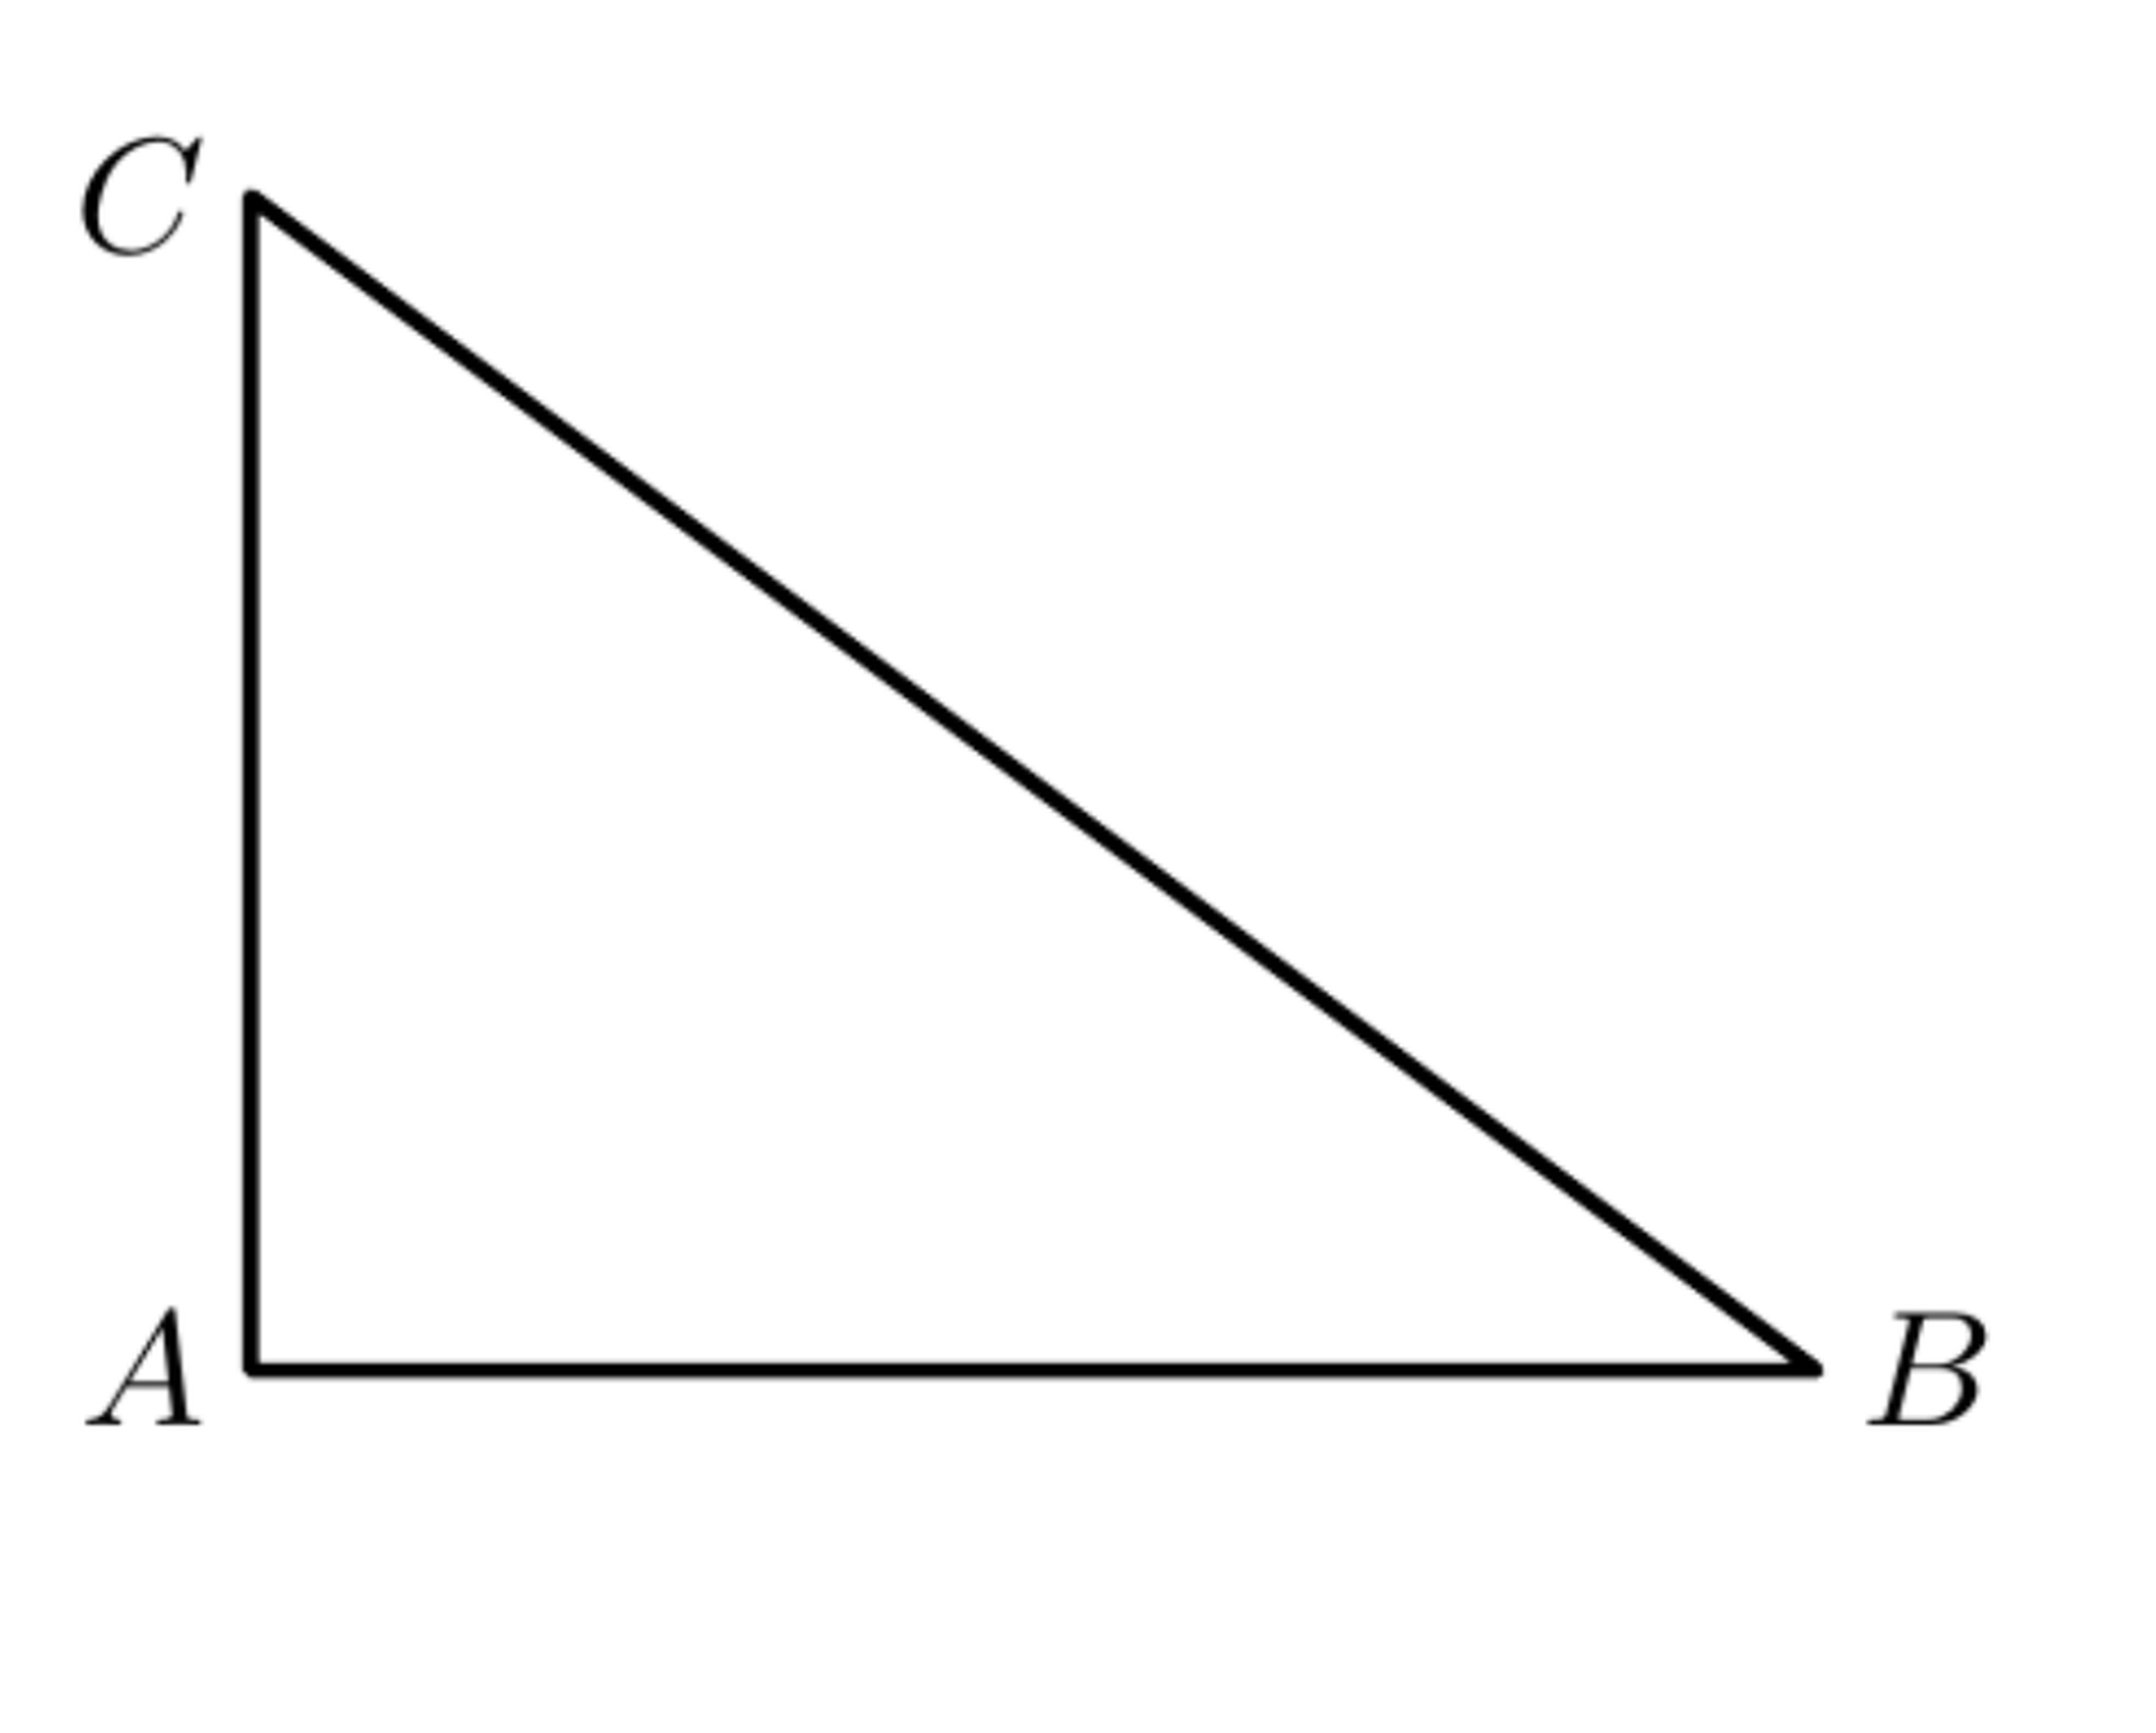
\includegraphics[width=0.34\textwidth]{figures/gao153_q19.png}
\end{center}

\ifanswer
\solbegin
\step{(1) 取 $A(0,0)$、$B(40,0)$、$C(0,30)$，则斜边 $BC$ 所在直线为 $3x+4y=120$.}
\step{正方形落在边界上的两边必分别在两条直角边上.}
\step{设其边长为 $a$m，则对角顶点为 $(a,a)$.}
\step{按题意划出的正方形应尽量大，即对角顶点落在斜边 $BC$ 上，}
\step{因此 $3a+4a=120\Rightarrow a=\dfrac{120}{7}$；}
\step{(2) 斜边长 $BC=\sqrt{30^2+40^2}=50$m，三角形面积为 $600\text{m}^2$.}
\step{设圆的半径为 $r$，圆心到 $AB$、$AC$、$BC$ 的距离分别为 $d_1,d_2,d_3$，}
\step{则三者均不小于 $r$. 连接圆心与三个顶点，}
\step{得 $600=\dfrac12(40d_1+30d_2+50d_3)\geqslant\dfrac12(40+30+50)r=60r$，所以 $r\leqslant10$.}
\step{取三角形的内切圆时等号成立，圆形区域面积的最大值为 $100\pi\text{m}^2$.}
\step{(3) 任取矩形落在绿地边界上的一边，以其所在直线为横轴.}
\step{设相应三角形底边长为 $L$、高为 $H$，则 $LH=1200$.}
\step{取三角形顶点坐标为 $(0,0)$、$(L,0)$、$(p,H)$.}
\step{在高度 $t$ 处，两腰上的点的横坐标分别为 $\dfrac{pt}{H}$、$L+\dfrac{(p-L)t}{H}$，}
\step{因此，高为 $t$ 的矩形，其底边长不超过 $L\left(1-\dfrac tH\right)$，}
\step{面积满足 $S\leqslant Lt\left(1-\dfrac tH\right)=\dfrac LH\left[\dfrac{H^2}{4}-\left(t-\dfrac H2\right)^2\right]\leqslant\dfrac{LH}{4}=300$，}
\step{在原坐标系中，取矩形顶点为 $(0,0)$、$(20,0)$、$(20,15)$、$(0,15)$，}
\step{其中 $3\times20+4\times15=120$，矩形完全位于绿地内，面积为 $300\text{m}^2$，}
\step{达到最大值.}
\solend
\fi

% === Q20 === $g(x)$ 定义照录；解析 14 行
\item 已知 $a>0$ 且 $a\ne1$，设 $f(x)=\log_a(x^2-a^2)$，$g(x)=2\log_a(x-ak)$.

(1) 求函数 $y=f(x)$ 的定义域；

(2) 若 $k=2$，求不等式 $f(x)>g(x)$ 的解集；

(3) 若“存在实数 $x$，使得 $f(x)=g(x)$”为真命题，求实数 $k$ 的取值范围.

\ifanswer
\solbegin
\step{(1) $x^2-a^2>0\Leftrightarrow x<-a$ 或 $x>a$，定义域为 $(-\infty,-a)\cup(a,+\infty)$.}
\step{(2) 两函数均有意义时，$x>2a$，且 $g(x)=\log_a(x-2a)^2$.}
\step{当 $a>1$ 时，$f(x)>g(x)\Leftrightarrow x^2-a^2>(x-2a)^2\Leftrightarrow x>\dfrac{5a}{4}$，}
\step{结合 $x>2a$，解集为 $(2a,+\infty)$.}
\step{当 $0<a<1$ 时，$f(x)>g(x)\Leftrightarrow x^2-a^2<(x-2a)^2\Leftrightarrow x<\dfrac{5a}{4}$，}
\step{与 $x>2a$ 矛盾，解集为 $\varnothing$.}
\step{(3) 在 $x^2-a^2>0$ 且 $x-ak>0$ 的条件下，}
\step{$f(x)=g(x)\Leftrightarrow x^2-a^2=(x-ak)^2\Leftrightarrow2akx=a^2(1+k^2)$，}
\step{当 $k=0$ 时，上式不成立；}
\step{当 $k\ne0$ 时，$x=\dfrac{a(1+k^2)}{2k}$，}
\step{于是 $x-ak=\dfrac{a(1-k^2)}{2k}>0\Leftrightarrow k<-1$ 或 $0<k<1$，}
\step{对上述 $k$，所取的 $x$ 同时满足 $x^2-a^2=(x-ak)^2>0$，}
\step{两函数均有意义且函数值相等.}
\step{因此，$k$ 的取值范围为 $(-\infty,-1)\cup(0,1)$.}
\solend
\fi

% === Q21 === 中文弯引号、复杂式照录；解析 23 行（跨 08→09 页）
\item 若实数 $x$、$y$、$m$ 满足 $\lvert x-m\rvert<\lvert y-m\rvert$，则称 $x$ 比 $y$ 接近 $m$.

(1) 若 $2x$ 比 $x-2$ 更接近 1，求实数 $x$ 的取值范围；

(2) 若 $x$ 比 $y$ 接近 $m$，证明：“$x>y$” 的充要条件是 “$x+y<2m$”；

(3) 已知 $x>0$，$y>0$ 且 $x\ne y$. 设 $p=\dfrac{x^2+y^2}{xy}$，若对于任意的 $x$、$y$，命题 “$p$ 比 $p^2-3p+4$ 接近 $m$” 恒成立，求实数 $m$ 的取值范围.

\ifanswer
\solbegin
\step{(1) $\lvert2x-1\rvert<\lvert x-3\rvert\Leftrightarrow(2x-1)^2<(x-3)^2\Leftrightarrow(x+2)(3x-4)<0$，}
\step{解得 $-2<x<\dfrac43$，实数 $x$ 的取值范围为 $\left(-2,\dfrac43\right)$.}
\step{(2) 因为 $x$ 比 $y$ 接近 $m$，所以 $\lvert x-m\rvert<\lvert y-m\rvert$，则 $\lvert x-m\rvert^2<\lvert y-m\rvert^2$，}
\step{即 $(x-m)^2<(y-m)^2$，即 $(x-m)^2-(y-m)^2<0$，}
\step{即得 $(x-y)(x+y-2m)<0$，}
\step{则由 $x+y<2m$，得 $x+y-2m<0$，}
\step{故 $x-y>0$，即 $x>y$，充分性成立；}
\step{当 $x>y$ 时，$x-y>0$，结合 $(x-y)(x+y-2m)<0$，得 $x+y-2m<0$，}
\step{即 $x+y<2m$，必要性成立；}
\step{故“$x>y$” 的充要条件是 “$x+y<2m$”；}
\step{(3) $x>0$，$y>0$ 且 $x\ne y$. 则 $p=\dfrac{x^2+y^2}{xy}=\dfrac xy+\dfrac yx>2\sqrt{\dfrac xy\cdot\dfrac yx}=2$，}
\step{由于对于任意的 $x$、$y$，命题 “$p$ 比 $p^2-3p+4$ 接近 $m$” 恒成立，}
\step{故 $\lvert p-m\rvert<\lvert(p^2-3p+4)-m\rvert$ 对 $\forall p>2$ 恒成立，}
\step{即得 $(p-m)^2<(p^2-3p+4-m)^2$，}
\step{即 $(p^2-3p+4-m)^2-(p-m)^2>0$，}
\step{得 $(p^2-4p+4)(p^2-2p+4-2m)>0$，}
\step{即 $(p-2)^2(p^2-2p+4-2m)>0$，由于 $p>2$，故 $(p-2)^2>0$，}
\step{故 $p^2-2p+4-2m>0$ 对 $\forall p>2$ 恒成立，}
\step{即 $2m<p^2-2p+4$ 对 $\forall p>2$ 恒成立，}
\step{由于 $p^2-2p+4=(p-1)^2+3$，此时 $p^2-2p+4$ 在 $(2,+\infty)$ 上严格增，}
\step{故 $(p-1)^2+3>(2-1)^2+3=4$，故 $2m\leqslant4$，解得 $m\leqslant2$，}
\step{即实数 $m$ 的取值范围是 $(-\infty,2]$.}
\solend
\fi

\end{enumerate}

\end{document}
"
%
% ① 原始材料：微信公众号"魔都数学加油站"文章，连载"27学年高一153"，原文标题
% "27学年高一153——2026-2027年上海市闵行中学文绮中学高一上期中"；
% 原文链接：https://mp.weixin.qq.com/s/rEtS-92cDR6JKgY2b5DRfg 。
% 正文为 9 张 PNG 页（01/02/06/07/08/09 为 2560×3620，03/04/05 为 4762×6735，
% 同一篇各页分辨率混排，逐页按各自分辨率裁图核对，别按预览比例换算裁框）。
% 体例：讲评版——填空 3—12（10 题）、选择 13—16（4 题）、解答 17—21（5 题），
% 共 19 题，自第 3 题起编；**全 19 题均印【解析】**（逐题核实，见 ② ②）。
% 题目、答案、解析均据原图转录；卷面粉红色水印"魔都数学加油站"及公众号页脚未录入。
% 全卷插图清单（逐页通读 9 页确认）：2 幅，均为题目配图、三版都出——
%   · Q11 正方形 OABC 曲线图（02 页右下：$y=5x^2$ 与 $y=x^{-\frac12}$ 两条曲线、
%     坐标轴、O/A/B/C/P/Q、正方形），裁 figures/gao153_q11.png；
%   · Q19 直角三角形 ABC 绿地示意图（05 页右上，直角在 A），
%     裁 figures/gao153_q19.png；
%   两图均去粉色水印、去色、4× LANCZOS 放大；Q11 图左上角题干残字"函"已裁白。
%   其余各页逐页确认无其它题目配图、无解析内配图、无表格；09 页下半仅水印、无正文。
%
% 卷首标题：原卷印作"2026-2027 年闵行中学文绮中学高一上期中"，年份区间按全稿惯例排 en dash；
% 原卷卷面未印副标题，本稿按同期中卷知识模块口径补出"集合与常用逻辑用语、不等式、函数"。
%
% ② 与原卷的排版差异：
%   ① 原文从第 3 题起，本稿保留原题号；共 19 题三节，解答题 5 题到 21；
%   ② 全 19 题均印【解析】、用 \solbegin…\solend，无只印【答案】或答案印括号内的题；
%      四道选择题答案在解析末句"故选 A／A／D／C"（Q13—Q16，逐个放大复核）、
%      括号 \mbox{（\quad）} 留空、不另提 \ans{}；答案版【答案】/【解析】标记数
%      = 19 = 全卷题数；
%   ③ 原卷卷面未印副标题，本稿按知识模块口径补出；
%   ④ 原卷填空横线按全稿惯例排 \blankline[4.4em]；选择题括号排 \mbox{（\quad）}、
%      四道选择题的选项段前按惯例各加 \keepwithprev；解答题不留作答区、不加
%      \anspace（原卷为讲评版，109—113 起全稿不用 \anspace）；
%   ⑤ 数集：Q3"$x\in R$"、Q5"解集为 R"、Q10"$x\in N$"、Q12"$x\in Z$"与
%      "$m\in Z$"、Q14"$m\in Z$"、Q16"$a\in N$"、Q17"全集 $U=R$"、
%      Q19 无、Q21 无——原卷印斜体或正体粗体 R/N/Z，按全稿惯例归一
%      \R／\N／\Z；绝对值排 \lvert…\rvert（Q5、Q11、Q21），集合描述竖线排 \mid
%      （Q3、Q10、Q17、Q20），不等号按全稿惯例排 \leqslant／\geqslant；
%      补集照原卷上划线排 \overline{A}（Q17 题干 (2)＋解析 (2)）；
%      空集 \varnothing（Q12 题干、Q20 解析 (2)）；子集 3 处均印带下划线 ⊆、
%      照录 \subseteq（Q10 $A\subseteq U$、Q12 $B\subseteq A$、Q17 $(-1,2)\subseteq(a-5,a)$），
%      本卷无单线 \subset 用例；
%   ⑥ 判别式：逐页通读 9 页，本卷无一元二次判别式 Δ/△ 算式，故无 Δ/△ 混用可照录；
%      Q11 图里有几何正方形 OABC（非三角形符号），无 △ABC 用例；
%   ⑦ 中文弯引号照录：Q14"$m=0$"与"幂函数…关于原点成中心对称"、
%      Q20"存在实数 $x$，使得 $f(x)=g(x)$"、Q21"$x>y$"与"$x+y<2m$"、
%      "$p$ 比 $p^2-3p+4$ 接近 $m$"（引号外留空格按原卷）；
%      注释里一律 ASCII 引号；数学式内 CJK 用 \text{}；
%   ⑧ "图像／图象"逐处放大核：全卷 3 处均印"图像"（像，有亻）——
%      Q13 题干与解析、Q14 题干与解析；Q19 题干写"如图所示"（非"图像"），
%      逐处照录未统一；子题标号 (1)(2)(3) 半角括号照录；圈数字本卷无用例；
%   ⑨ 半角逗号在数学组之间是全稿惯例、非笔误，逐处照录（Q3 $x\in R$、
%      Q10 $a_1,a_2$、Q19 $A(0,0)$、$d_1,d_2,d_3$、Q21 $a>\frac13,b>\frac13$ 等）；
%      行末西文句点 ASCII `.`；行中全角逗号／顿号照录（Q19"30m 和 40m"、
%      Q21"实数 $x$、$y$、$m$"）；
%   ⑩ 复杂式照录别简化：Q3 $y=x^{-2}$、Q11 $y=x^{-\frac12}$ 与
%      $\frac{2}{\sqrt[4]{5}}$、Q8 $\frac{2b}{a+1-b}$、Q9 cases 块、
%      Q10 $525=5\times105$、Q16 $a^2+1$、Q19 $S\leqslant Lt(1-\frac tH)$
%      与 $L+\frac{(p-L)t}{H}$、Q20 $2akx=a^2(1+k^2)$ 与 $\frac{a(1+k^2)}{2k}$、
%      Q21 $(p^2-4p+4)(p^2-2p+4-2m)>0$；
%      \left…\right 不得拆到不同 $…$ 组（Q17 $\left\{x\mid\cdots\right\}$、
%      Q19 $\left[\frac{H^2}{4}-\left(t-\frac H2\right)^2\right]$、
%      Q21 $\left(-2,\frac43\right)$ 等）；cases 块一律 \begin{cases}…\end{cases}；
%   ⑪ 一条 \step = 原卷解析的一个印刷行，cases 块整体算一个印刷行；别并折行、
%      别拆行。Q10 六行、Q19 十九行、Q20 十四行、Q21 二十二行均按印刷行逐条断，
%      不丢行；
%   ⑫ 配图：Q11／Q19 题目配图（三版都出）放 \item 内题干之后 \begin{center}，
%      各用 \needvspace{8cm} 守卫把整块推走，**守卫放在 \item 之前**
%      （见 高一145 Q14/Q20 成例与切页审计 B 类坑）；
%   ⑬ 原卷解析内无红色"法一／法二"之类小标题，故本卷无 \stepm；红色水印
%      "魔都数学加油站"不录入；
%   ⑭ 跨页续印按题合并：见 ⑥；
%
% ③ 行数复核：一条 \step = 原卷解析的一个印刷行，cases 块作一个印刷行计。
%   逐题数（主会话逐页核对定稿）：Q3：1；Q4：2；Q5：2；Q6：2；Q7：1；
%   Q8：1；Q9：2；Q10：6；Q11：3；Q12：5；Q13：2；Q14：3；Q15：5；
%   Q16：3；Q17：5；Q18：4；Q19：19；Q20：14；Q21：22。
%   合计 102 条 \step（本卷无 \stepm），与原卷逐题印刷行相等。全卷 19 题
%   均设 \solbegin…\solend，答案版【答案】/【解析】标记数 = 19 = 全卷题数。
%
% ④ 判别式／子集符号结论（逐处放大原图照录、不得统一，主会话像素级复核）：
%   判别式：逐页通读 9 页，本卷无一元二次判别式算式（Q7 用韦达定理、
%      Q16 用因式分解、Q20 用对数方程，均不写 Δ/△），故无 Δ/△ 混用可照录
%      （"高 \Delta／扁 \triangle"口径备查，参照 高一142／151／152 头注）；
%      本卷无几何三角形符号用例。
%   子集：Q10 题干"$A\subseteq U$"、Q12 题干"$B\subseteq A$"、Q17 解析 (2)
%      "$(-1,2)\subseteq(a-5,a)$"共 3 处，逐处放大确认均印带下划线 ⊆、
%      照录 \subseteq；本卷未见单线 ⊂（\subset）之对应处。
%      补集上划线 \overline{A}（Q17）、空集 \varnothing（Q12 题干、Q20 解析 (2)）；
%      数集 \R／\N／\Z 归一见 ② ⑤。
%
% ⑤ 存疑照录（放大原图确认，照录未改、正文对应处另有 % 注）：
%   1. Q3 集合 $B=\{(x,y)\mid y=x^{-2},x\in\R\}$ 原卷题干径写 $x\in\R$
%      （$x=0$ 处无意义），解析自行注明 $x\ne0$，照录未改。
%   2. Q10 解析"$U$ 中共有 $525=5\times105$ 个连续整数"与尾行
%      "取 $U$ 中除以 5 余 1 或 2 的全部元素及元素 5"逐字照录（放大 02 页
%      /tmp/gao153/z/zoom/q10_pick.png 确认是"元素 5"，非"元素 9"）。
%   3. Q11 第二个函数原卷印 $y=x^{-\frac12}$（负二分之一次幂，非 $x^2$），
%      放大 02 页 /tmp/gao153/z/zoom/q11_exp.png 确认，照录未改；
%      $|AQ|=\frac1{\sqrt a}$ 与之自洽。
%   4. Q19 (3) 解析"在高度 $t$ 处，两腰上的点的横坐标分别为 $\frac{pt}{H}$、
%      $L+\frac{(p-L)t}{H}$"，放大 06 页确认，照录未简化。
%   5. Q20 (2) 解析"$g(x)=\log_a(x-2a)^2$"（真数整体平方），
%      与 $g(x)=2\log_a(x-ak)$ 在 $k=2$ 时一致，照录未改。
%   6. Q21 (3) 解析"得 $(p^2-4p+4)(p^2-2p+4-2m)>0$"与
%      "故 $(p-1)^2+3>(2-1)^2+3=4$，故 $2m\leqslant4$"照录未改
%      （放大 09 页 /tmp/gao153/z/zoom/q21_factor.png 确认）。
%   7. "图像／图象"全卷 3 处均印"图像"（像，有亻）逐处照录；
%      本卷无判别式 Δ/△ 用例（见 ④）。
%   全卷除此 7 类外未发现其它笔误／自相矛盾处；19 题均印【解析】、
%   无只印【答案】或答案印括号内的题（见 ② ②）。
%
% ⑥ 跨页续印按题合并说明（逐页核实定稿）：Q3—Q5 题干＋解析在 01 页；
%   Q6—Q8 题干＋解析在 01 页下半（Q8 解析续 02 页顶）；Q9 题干＋解析、
%   Q10 题干＋解析首 2 行在 02 页上半，Q10 解析余 4 行在 02 页下半；
%   Q11 题干＋配图＋解析、Q12 题干＋解析 5 行在 02 页下半—03 页上半；
%   "二、选择题"标题在 03 页中部；Q13 题干＋选项＋解析在 03 页下半；
%   Q14 题干＋选项＋解析、Q15 题干＋选项＋解析首行在 03 页下半—04 页顶；
%   Q15 解析余 4 行、Q16 题干＋选项＋解析在 04 页上半；"三、解答题"
%   标题在 04 页下半；Q17 题干＋两问＋解析 5 行在 04 页下半—05 页顶；
%   Q18 题干＋两问＋解析 4 行、Q19 题干（含配图）＋三问在 05 页；
%   Q19 解析 (1)(2) 9 行在 05 页下半，解析 (3) 前 5 行在 06 页上半、
%   余 4 行在 06 页下半；Q20 题干＋三问在 06 页下半，解析 (1)(2)(3)
%   前 6 行在 07 页上半、(3) 余 8 行在 07 页下半；Q21 题干＋三问在
%   07 页末，解析 (1)(2) 10 行在 08 页上半—下半，解析 (3) 前 4 行在
%   08 页下半、余 9 行续 09 页上半，末行"即实数 $m$ 的取值范围是
%   $(-\infty,2]$"为全卷收尾（09 页下半仅水印、无正文）。
%   本稿按题连排，不丢行、不并折行；全卷末题为第 21 题，无附加题节。
%
\documentclass[a4paper,11pt]{article}
\usepackage{common}

\begin{document}

\examtitlest[3]{2026--2027 年闵行中学文绮中学高一上期中}{集合与常用逻辑用语、不等式、函数}

\bigsec{一、填空题}

\begin{enumerate}
\setcounter{enumi}{2}

% === Q3 === 集合描述竖线 \mid；$y=x^{-2}$ 照录；解析 1 行
\item 已知 $A=\{(x,y)\mid y=x^3,x\in\R\}$，$B=\{(x,y)\mid y=x^{-2},x\in\R\}$，则 $A\cap B=$\blankline[4.4em].

\ifanswer
\solbegin
\step{$x^3=x^{-2}\ (x\ne0)\Leftrightarrow x^5=1\Leftrightarrow x=1$，此时 $y=1$，所以 $A\cap B=\{(1,1)\}$.}
\solend
\fi

% === Q4 === 解析 2 行
\item 若关于 $x$ 的不等式 $\dfrac{x-a}{x+1}>0$ 的解集为 $(-\infty,-1)\cup(4,+\infty)$，则实数 $a=$\blankline[4.4em].

\ifanswer
\solbegin
\step{关于 $x$ 的不等式 $\dfrac{x-a}{x+1}>0$ 即 $(x+1)(x-a)>0$.}
\step{再由它的解集为 $(-\infty,-1)\cup(4,+\infty)$，得 $-1$ 和 4 是 $(x+1)(x-a)=0$ 的两个实数根，故 $a=4$.}
\solend
\fi

% === Q5 === 绝对值 \lvert…\rvert；解析 2 行
\item 若关于 $x$ 的不等式 $\lvert x+1\rvert+\lvert x-2\rvert>m$ 的解集为 $\R$，则实数 $m$ 的取值范围是\blankline[4.4em].

\ifanswer
\solbegin
\step{$\lvert x+1\rvert+\lvert x-2\rvert\geqslant\lvert(x+1)-(x-2)\rvert=3$，当且仅当 $-1\leqslant x\leqslant2$ 时取等号，}
\step{因此 $m<3$.}
\solend
\fi

% === Q6 === 解析 2 行
\item 已知指数函数 $y=a^x$（$a>1$）在区间 $[-1,1]$ 上的最大值比最小值大 $\dfrac32$，则实数 $a=$\blankline[4.4em].

\ifanswer
\solbegin
\step{$a>1$，指数函数在 $[-1,1]$ 上严格增，故 $a-\dfrac1a=\dfrac32\Leftrightarrow(a-2)(2a+1)=0$.}
\step{结合 $a>1$，得 $a=2$.}
\solend
\fi

% === Q7 === 韦达定理；解析 1 行
\item 已知关于 $x$ 的一元二次方程 $x^2+px+2p=0$ 的两个实数根分别为 $x_1$、$x_2$，且 $(x_1+1)(x_2+1)=0$，则 $p=$\blankline[4.4em].

\ifanswer
\solbegin
\step{$0=(x_1+1)(x_2+1)=x_1x_2+x_1+x_2+1=2p-p+1=p+1\Rightarrow p=-1$.}
\solend
\fi

% === Q8 === 换底公式；解析 1 行
\item 已知 $10^a=3$，$\lg5=b$，则 $\log_6 25=$\blankline[4.4em]（用关于 $a,b$ 的关系式表示）.

\ifanswer
\solbegin
\step{$\lg3=a$，$\lg2=1-b$，所以 $\log_6 25=\dfrac{\lg25}{\lg6}=\dfrac{2b}{a+1-b}$.}
\solend
\fi

% === Q9 === cases 块整体算一个印刷行；解析 2 行
\item 已知 $A=[2,5]$，若对任意 $x\in A$，总有 $\dfrac{k}{x}\in A$，则正数 $k=$\blankline[4.4em].

\ifanswer
\solbegin
\step{$k>0$，当 $x\in[2,5]$ 时，$\dfrac{k}{x}$ 的取值范围为 $\left[\dfrac k5,\dfrac k2\right]$，}
\step{因此 $\begin{cases}\dfrac k5\geqslant2\\\dfrac k2\leqslant5\end{cases}\Leftrightarrow10\leqslant k\leqslant10\Leftrightarrow k=10$.}
\solend
\fi

% === Q10 === $A\subseteq U$ 带下划线照录；解析 6 行
\item 已知集合 $U=\{x\mid4\leqslant x\leqslant528,x\in\N\}$，$A=\{a_1,a_2,a_3,\cdots,a_n\}$，且 $A\subseteq U$. 如果集合 $A$ 中的任意两个不同元素之和都不能被 5 整除，则正整数 $n$ 的最大值为\blankline[4.4em].

\ifanswer
\solbegin
\step{$U$ 中共有 $525=5\times105$ 个连续整数，按除以 5 的余数分成五类，}
\step{每类均有 105 个元素.}
\step{余数为 1,4 的两类不能同时选取，余数为 2,3 的两类也不能同时选取，}
\step{余数为 0 的一类最多选 1 个，因此 $n\leqslant105+105+1=211$.}
\step{取 $U$ 中除以 5 余 1 或 2 的全部元素及元素 5，}% 放大 02 页确认是「元素 5」（非 9），照录未改（见 ⑤ 2）
\step{任意两个不同元素之和均不能被 5 整除，此时 $n=211$，最大值为 211.}
\solend
\fi

% === Q11 === 题目配图（三版都出）；\needvspace 守卫放 \item 之前；$y=x^{-\frac12}$ 照录；解析 3 行
\needvspace{8cm}
\item 如图，已知正方形 $OABC$，其中 $OA=a$（$a>1$），函数 $y=5x^2$ 交 $BC$ 于点 $P$，函数 $y=x^{-\frac12}$ 交 $AB$ 于点 $Q$，当 $\lvert AQ\rvert+\lvert CP\rvert$ 最小时，$a$ 的值为\blankline[4.4em].

\begin{center}
% 正方形 OABC 与两条曲线图取 02 页右下，去粉色水印、去色、4× LANCZOS 放大；三版都出
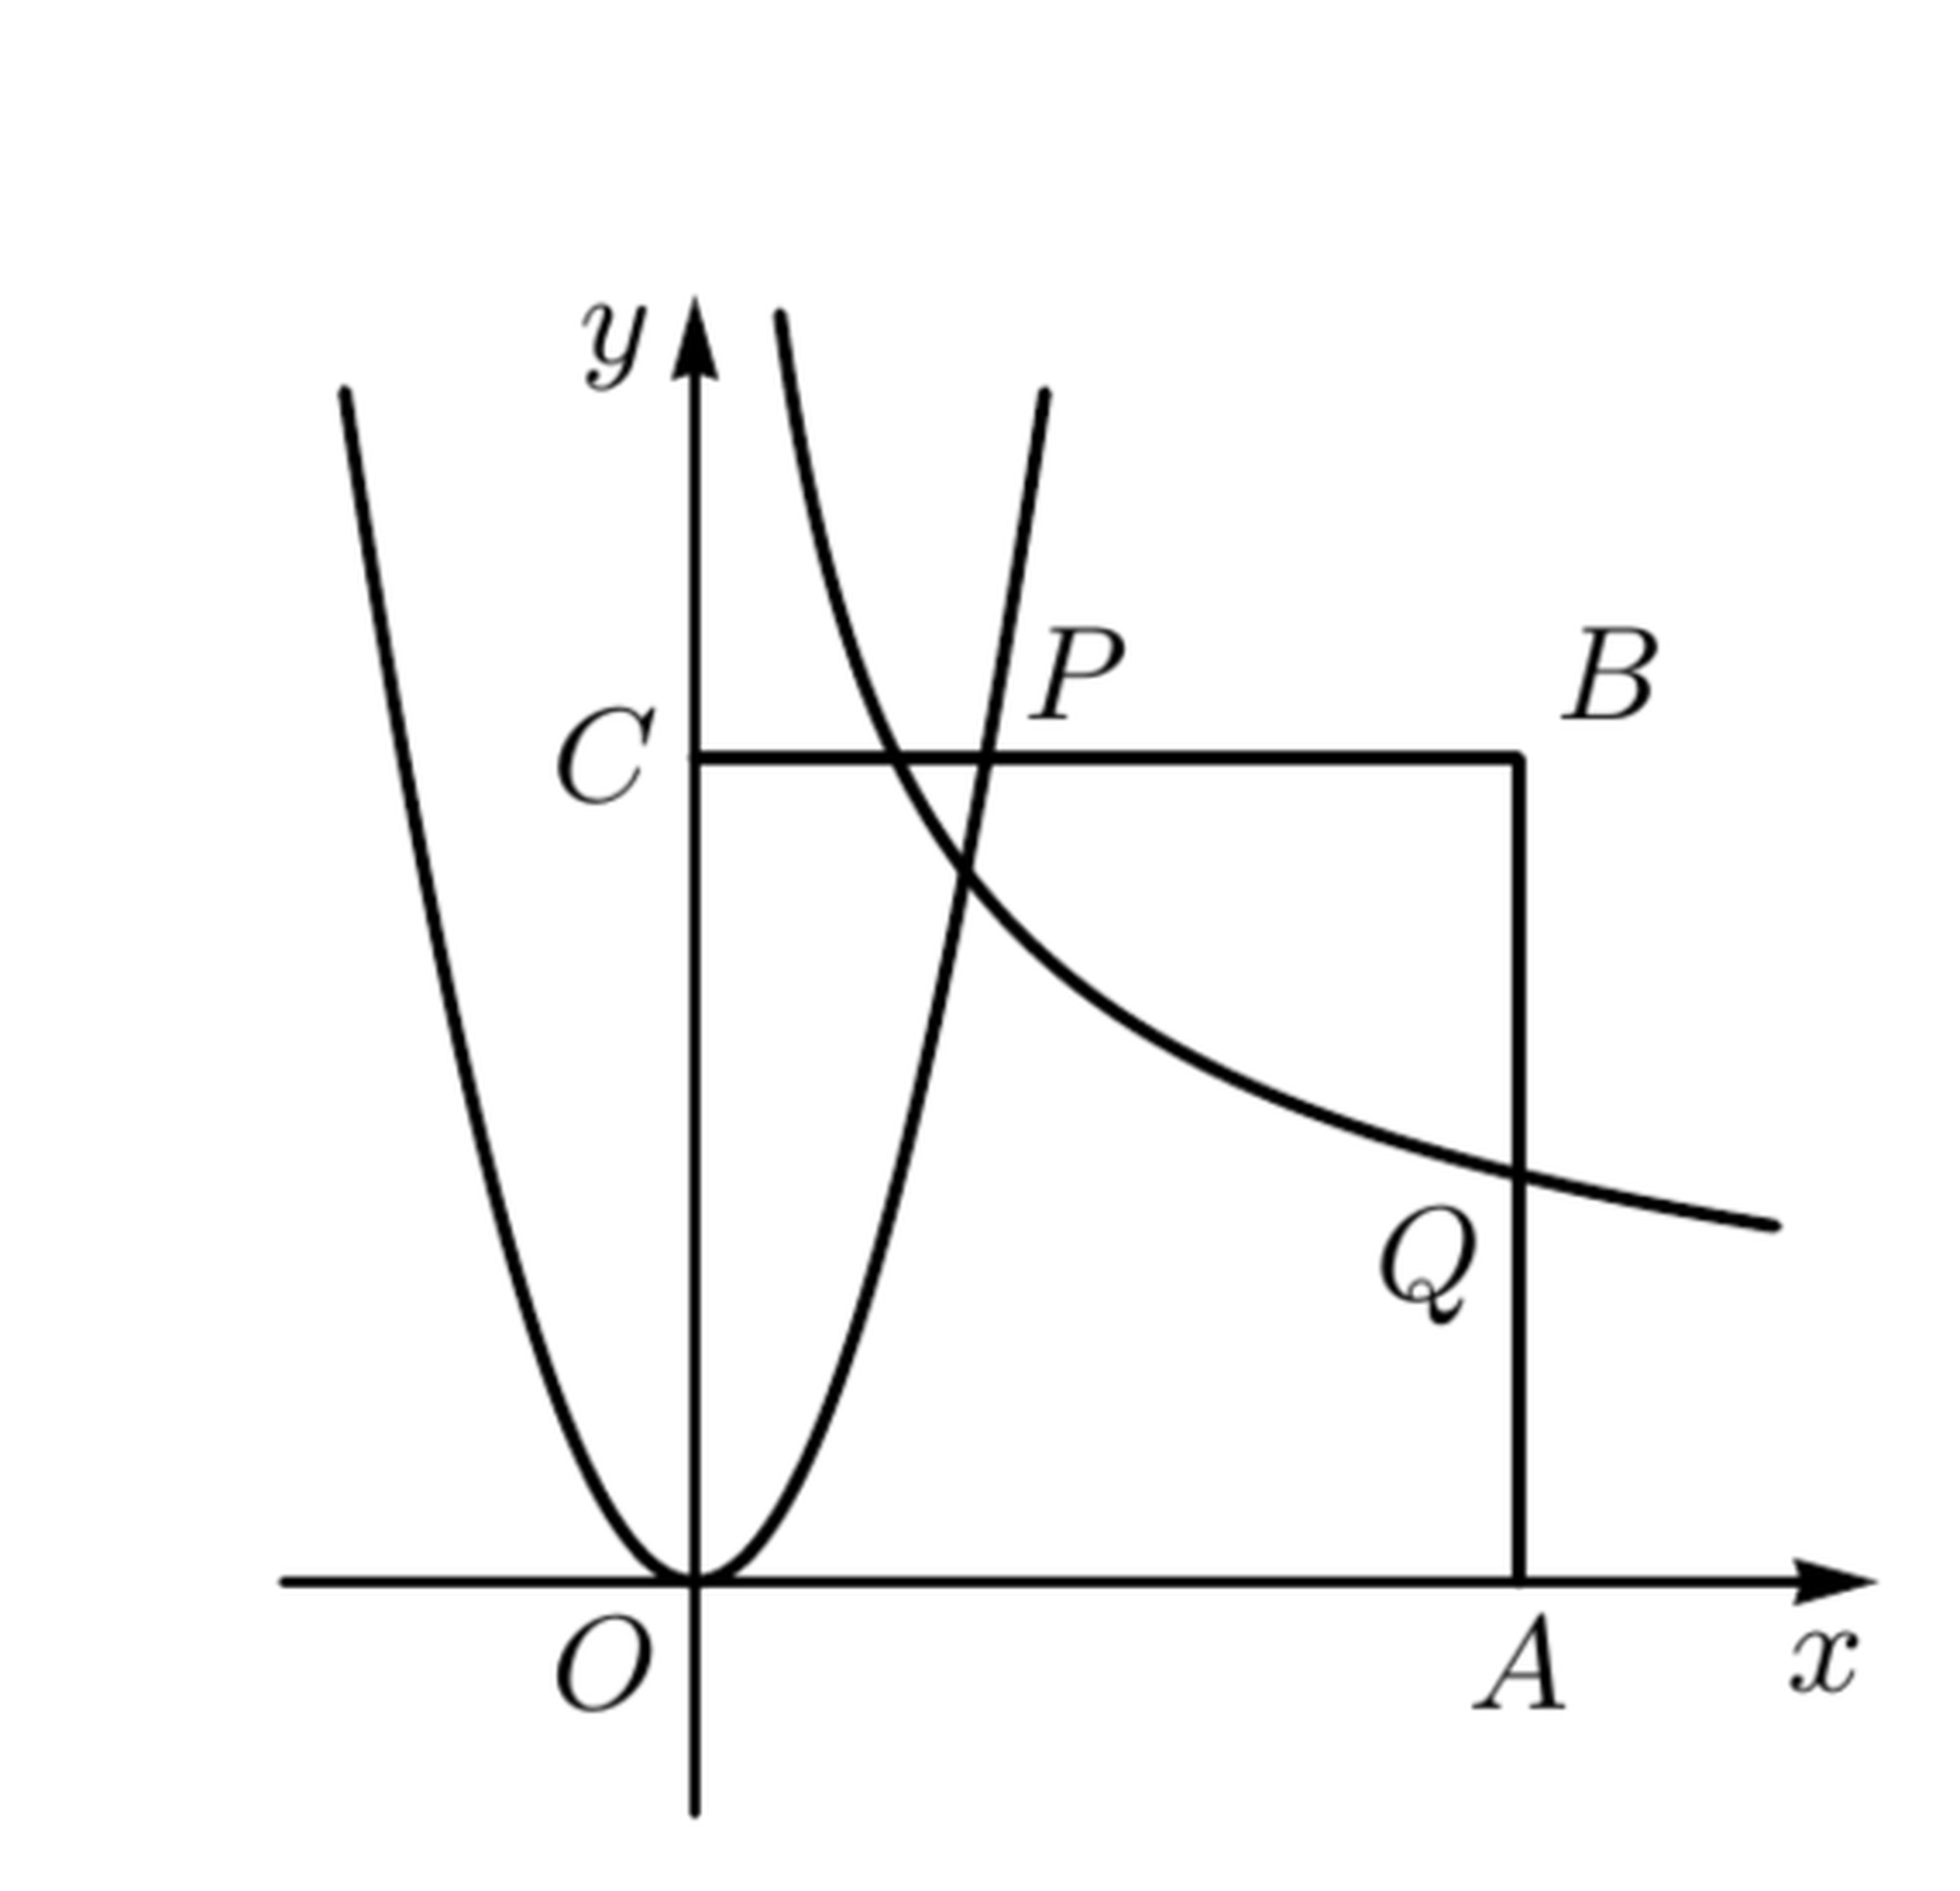
\includegraphics[width=0.40\textwidth]{figures/gao153_q11.png}
\end{center}

\ifanswer
\solbegin
\step{$\lvert AQ\rvert=\dfrac1{\sqrt a}$，$\lvert CP\rvert=\sqrt{\dfrac a5}$，}
\step{于是 $\lvert AQ\rvert+\lvert CP\rvert=\dfrac1{\sqrt a}+\sqrt{\dfrac a5}\geqslant2\sqrt{\dfrac1{\sqrt a}\cdot\sqrt{\dfrac a5}}=\dfrac2{\sqrt[4]{5}}$，}
\step{当且仅当 $\dfrac1{\sqrt a}=\sqrt{\dfrac a5}$，即 $a=\sqrt5$ 时取等号.}
\solend
\fi

% === Q12 === $B\subseteq A$ 带下划线照录、空集 \varnothing；解析 5 行
\item 若集合 $A=\{x\mid1\leqslant x\leqslant100,x\in\Z\}$，集合 $B\subseteq A$，且 $B\ne\varnothing$，记 $W(B)$ 为 $B$ 中元素的最大值与最小值之和，则对所有的 $B$，$W(B)$ 的平均值是\blankline[4.4em].

\ifanswer
\solbegin
\step{对每个非空子集 $B$，令 $B'=\{101-x\mid x\in B\}$，}
\step{则 $W(B')=(101-\min B)+(101-\max B)=202-W(B)$.}
\step{对 $B'$ 再作同样变换即得到 $B$，因此 $B$ 遍历所有非空子集时，}
\step{$B'$ 也恰好遍历所有非空子集.}
\step{设所求平均值为 $m$，则 $m=202-m$，解得 $m=101$.}
\solend
\fi

\end{enumerate}

\bigsec{二、选择题}

\begin{enumerate}
\setcounter{enumi}{12}

% === Q13 === "图像"（像，有亻）照录；解析 2 行，故选 A
\item 设 $a$、$b$ 为常数，若 $0<a<1$，$b>1$，则函数 $y=a^x-b$ 的图像必定不经过\mbox{（\quad）}

\keepwithprev
A. 第一象限\qquad\qquad B. 第二象限\qquad\qquad C. 第三象限\qquad\qquad D. 第四象限

\ifanswer
\solbegin
\step{当 $x>0$ 时，$a^x<1<b$，所以 $y=a^x-b<0$，图像必定不经过第一象限，}
\step{故选 $A$.}
\solend
\fi

% === Q14 === $m\in\Z$、中文弯引号、"图像"照录；解析 3 行，故选 A
\item 已知 $m\in\Z$，则“$m=0$”是“幂函数 $y=x^{m^2-2m-1}$ 的图像与 $x$ 轴及 $y$ 轴均无交点，且关于原点成中心对称”的\mbox{（\quad）}

\keepwithprev
A. 充分不必要条件\qquad\qquad B. 必要不充分条件

C. 充要条件\qquad\qquad D. 既不充分也不必要条件

\ifanswer
\solbegin
\step{图像满足所述条件 $\Leftrightarrow m^2-2m-1$ 为负奇数 $\Leftrightarrow m=0$ 或 $m=2$.}
\step{$m=0$ 能推出所述条件，但所述条件不能推出 $m=0$，因此是充分不必要条件，}
\step{故选 $A$.}
\solend
\fi

% === Q15 === 四选项一行；解析 5 行（跨 03→04 页），故选 D
\item 设 $a>b>1$，$x>1$，则下列不等式正确的是\mbox{（\quad）}

\keepwithprev
A. $a^x<b^x$\qquad B. $x^a<x^b$\qquad C. $\log_a x>\log_b x$\qquad D. $\log_x a>\log_x b$

\ifanswer
\solbegin
\step{$x>1$，幂函数与指数函数的单调性给出 $a^x>b^x$，$x^a>x^b$，A、B 错误.}
\step{$\log_a x=\dfrac{\lg x}{\lg a}<\dfrac{\lg x}{\lg b}=\log_b x$，C 错误.}
\step{对数函数 $y=\log_x t$ 的底数 $x>1$，在 $(0,+\infty)$ 上严格递增，}
\step{所以 $\log_x a>\log_x b$，D 正确.}
\step{故选 $D$.}
\solend
\fi

% === Q16 === $a\in\N$；解析 3 行，故选 C
\item 设 $a\in\N$，则满足不等式 $x^2-a^2x-a^2-1<0$ 的整数 $x$ 的个数不可能是\mbox{（\quad）}

\keepwithprev
A. 1\qquad\qquad B. 50\qquad\qquad C. 100\qquad\qquad D. 2026

\ifanswer
\solbegin
\step{$(x+1)(x-a^2-1)<0\Leftrightarrow-1<x<a^2+1$. 整数解为 $0,1,\cdots,a^2$，共 $a^2+1$ 个.}
\step{$1=0^2+1$，$50=7^2+1$，$2026=45^2+1$，而 $100-1=99$ 不是完全平方数，}
\step{故选 $C$.}
\solend
\fi

\end{enumerate}

\bigsec{三、解答题}

\begin{enumerate}
\setcounter{enumi}{16}

% === Q17 === 补集上划线 \overline{A}、\subseteq 照录；解析 5 行
\item 已知全集 $U=\R$，集合 $A=\{x\mid x^2-x-2\geqslant0\}$，$B=\{x\mid x>-1\}$，$C=\{x\mid a-5<x<a\}$.

(1) 求 $A\cap B$、$A\cup B$；

(2) 若 $\overline{A}\cup C=C$，求实数 $a$ 的取值范围.

\ifanswer
\solbegin
\step{(1) $x^2-x-2=(x+1)(x-2)\geqslant0\Leftrightarrow x\leqslant-1$ 或 $x\geqslant2$，}
\step{所以 $A=(-\infty,-1]\cup[2,+\infty)$，$B=(-1,+\infty)$，}
\step{因此 $A\cap B=[2,+\infty)$，$A\cup B=\R$.}
\step{(2) $\overline{A}=(-1,2)$，于是 $\overline{A}\cup C=C\Leftrightarrow\overline{A}\subseteq C\Leftrightarrow(-1,2)\subseteq(a-5,a)$，}
\step{两区间均为开区间，端点可重合，故 $\begin{cases}a-5\leqslant-1\\a\geqslant2\end{cases}\Leftrightarrow2\leqslant a\leqslant4$.}
\solend
\fi

% === Q18 === 解析 4 行
\item 已知 $a$、$b$、$c$ 都是正数，

(1) 若 $a+b=1$，求证：$\dfrac1a+\dfrac1b\geqslant4$，并指出等号成立的条件；

(2) 若 $a+b+c=1$，求证：三个数 $\dfrac1a$、$\dfrac1b$、$\dfrac1c$ 中至少有一个不小于 3.

\ifanswer
\solbegin
\step{(1) 由 $(a-b)^2\geqslant0$，得 $4ab\leqslant(a+b)^2=1$，所以 $\dfrac1a+\dfrac1b=\dfrac{a+b}{ab}=\dfrac1{ab}\geqslant4$，}
\step{等号成立当且仅当 $a=b$，结合 $a+b=1$，得 $a=b=\dfrac12$.}
\step{(2) 假设三个数 $\dfrac1a$、$\dfrac1b$、$\dfrac1c$ 都小于 3，则 $a>\dfrac13,b>\dfrac13,c>\dfrac13\Rightarrow a+b+c>1$，}
\step{与 $a+b+c=1$ 矛盾，因此三个数中至少有一个不小于 3.}
\solend
\fi

% === Q19 === 题目配图（三版都出）；\needvspace 守卫放 \item 之前；解析 19 行
\needvspace{8cm}
\item 某新建居民小区有一直角三角形绿地，两直角边长分别为 30m 和 40m，打算在其中划出一片区域改造成活动场地，如图所示.

(1) 若划出的区域为正方形，且有两边落在绿地边界上，求此正方形边长；

(2) 若划出的区域为圆形，求圆形区域面积的最大值；

(3) 若划出的区域为矩形（其中至少有一边在边界上），求此矩形面积的最大值.

\begin{center}
% 直角三角形 ABC 绿地示意图取 05 页右上，去粉色水印、去色、4× LANCZOS 放大；三版都出
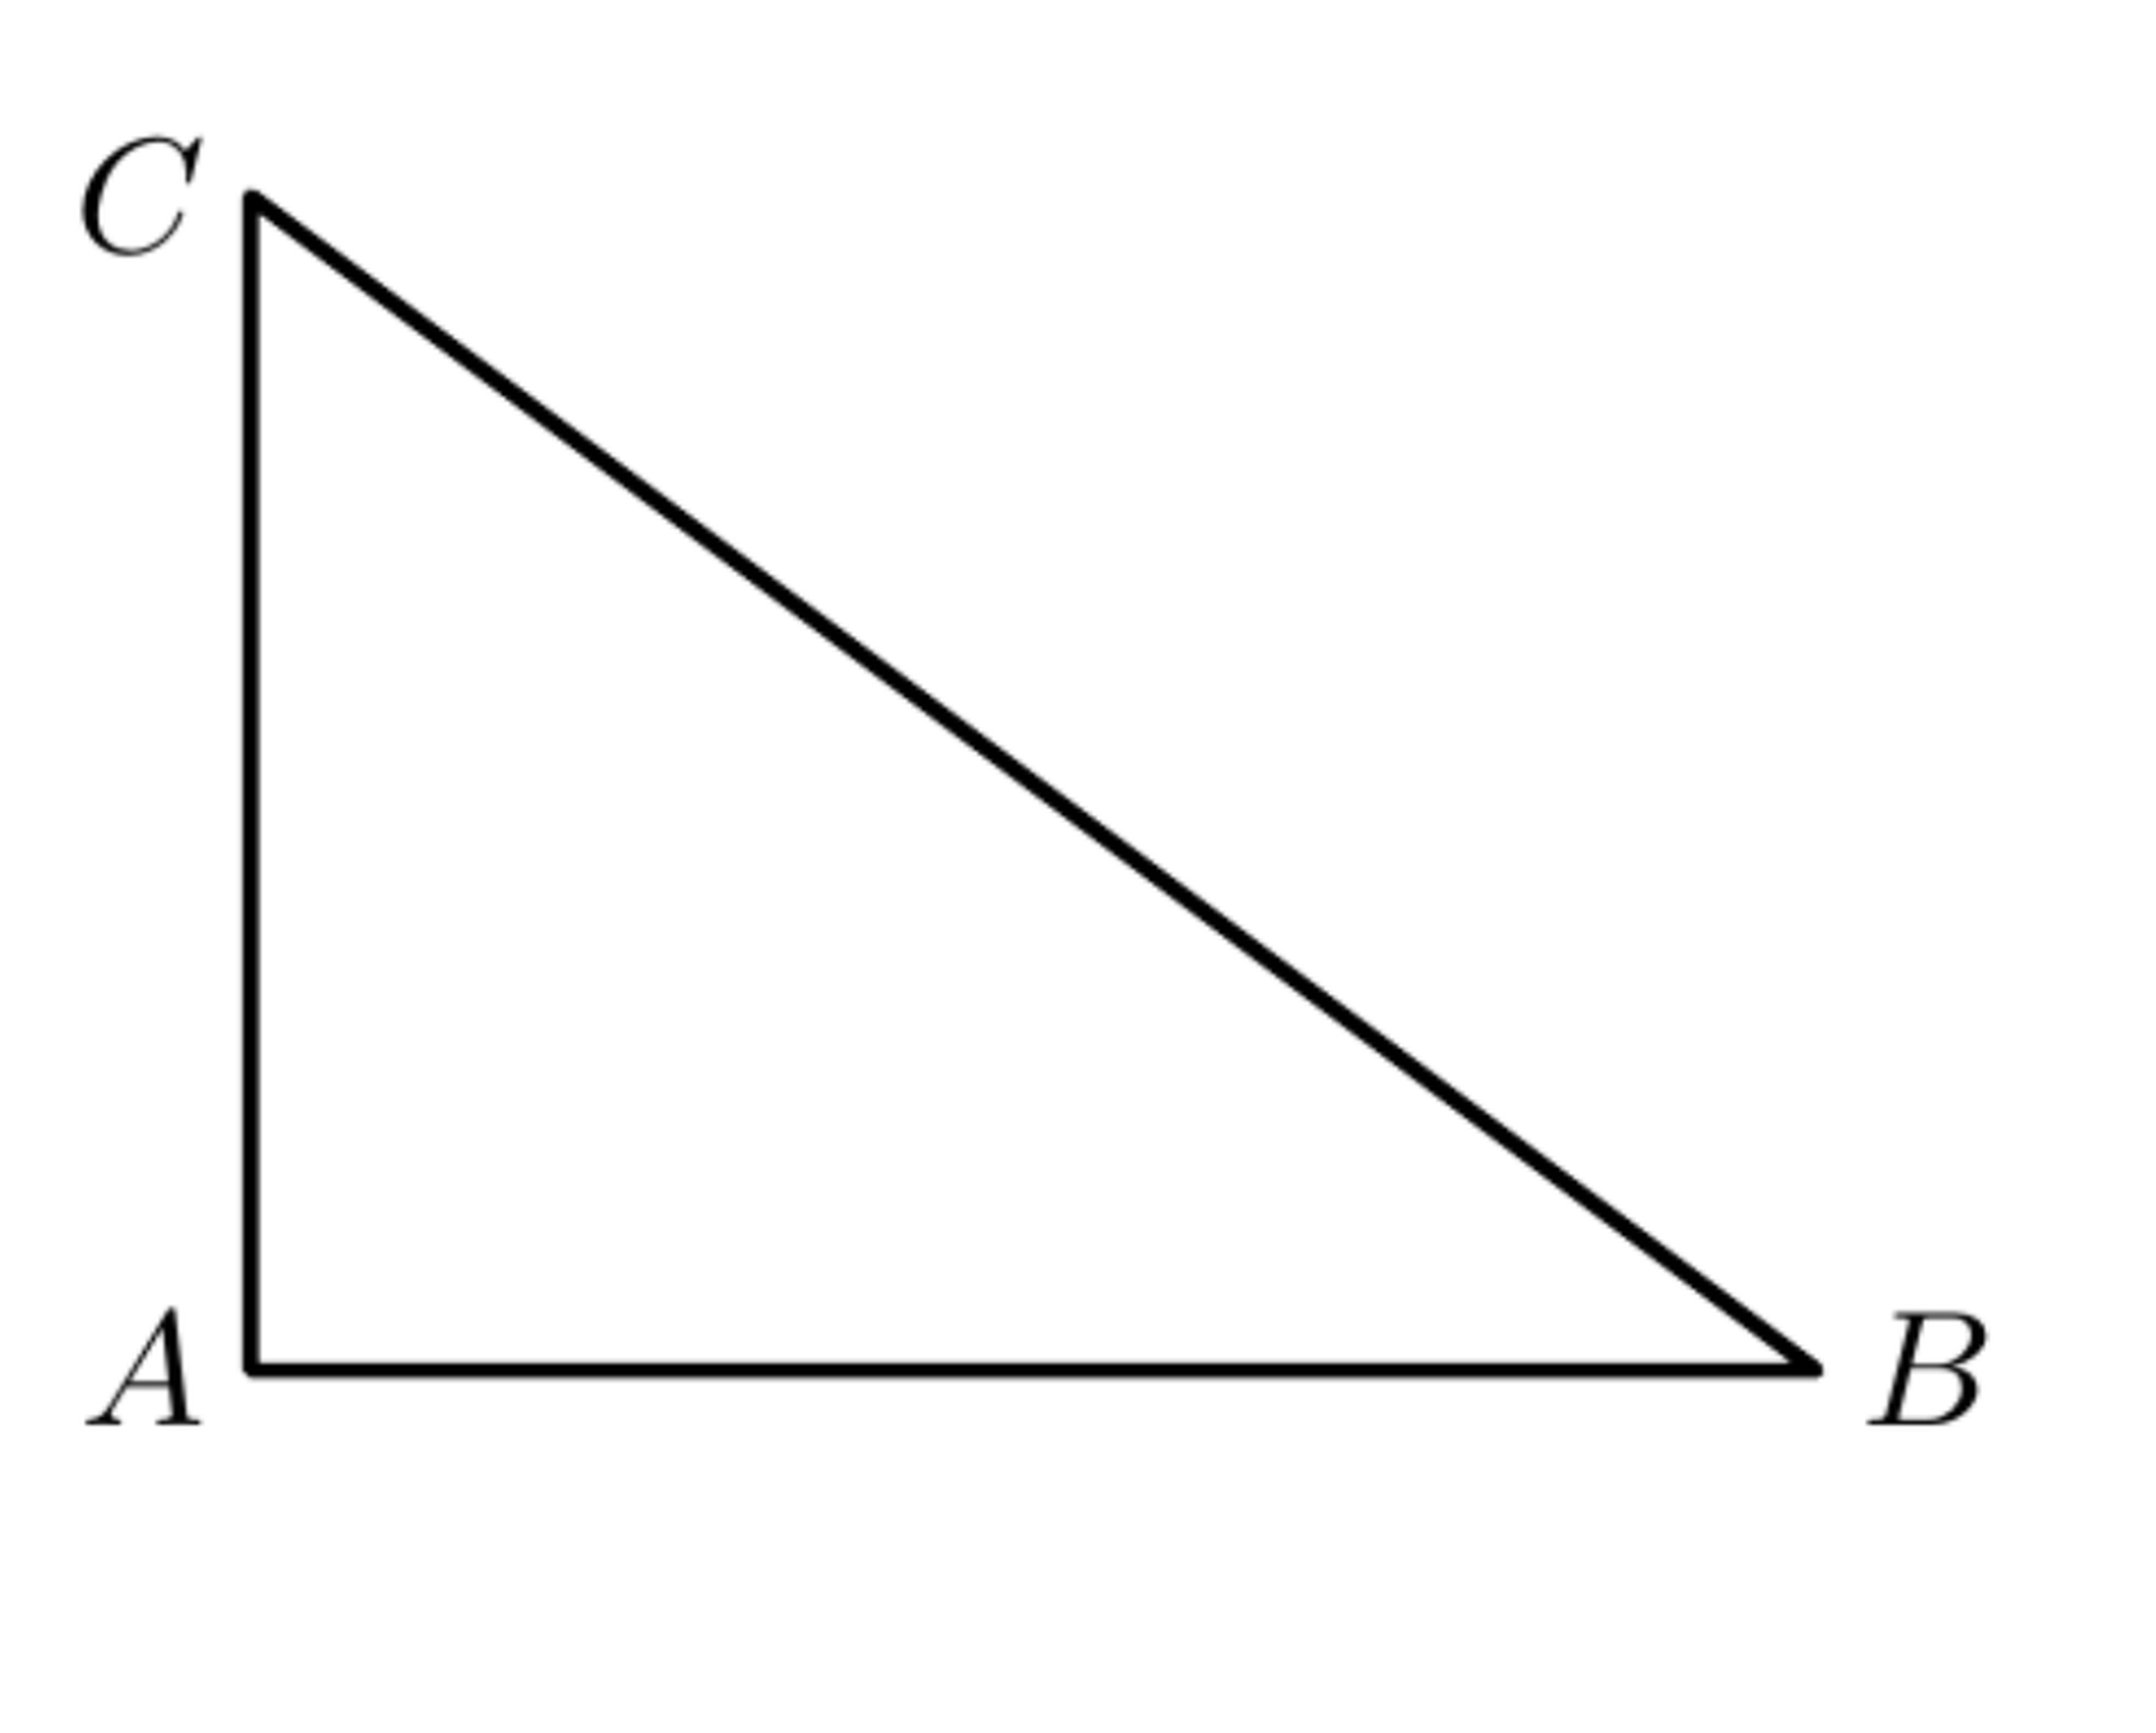
\includegraphics[width=0.34\textwidth]{figures/gao153_q19.png}
\end{center}

\ifanswer
\solbegin
\step{(1) 取 $A(0,0)$、$B(40,0)$、$C(0,30)$，则斜边 $BC$ 所在直线为 $3x+4y=120$.}
\step{正方形落在边界上的两边必分别在两条直角边上.}
\step{设其边长为 $a$m，则对角顶点为 $(a,a)$.}
\step{按题意划出的正方形应尽量大，即对角顶点落在斜边 $BC$ 上，}
\step{因此 $3a+4a=120\Rightarrow a=\dfrac{120}{7}$；}
\step{(2) 斜边长 $BC=\sqrt{30^2+40^2}=50$m，三角形面积为 $600\text{m}^2$.}
\step{设圆的半径为 $r$，圆心到 $AB$、$AC$、$BC$ 的距离分别为 $d_1,d_2,d_3$，}
\step{则三者均不小于 $r$. 连接圆心与三个顶点，}
\step{得 $600=\dfrac12(40d_1+30d_2+50d_3)\geqslant\dfrac12(40+30+50)r=60r$，所以 $r\leqslant10$.}
\step{取三角形的内切圆时等号成立，圆形区域面积的最大值为 $100\pi\text{m}^2$.}
\step{(3) 任取矩形落在绿地边界上的一边，以其所在直线为横轴.}
\step{设相应三角形底边长为 $L$、高为 $H$，则 $LH=1200$.}
\step{取三角形顶点坐标为 $(0,0)$、$(L,0)$、$(p,H)$.}
\step{在高度 $t$ 处，两腰上的点的横坐标分别为 $\dfrac{pt}{H}$、$L+\dfrac{(p-L)t}{H}$，}
\step{因此，高为 $t$ 的矩形，其底边长不超过 $L\left(1-\dfrac tH\right)$，}
\step{面积满足 $S\leqslant Lt\left(1-\dfrac tH\right)=\dfrac LH\left[\dfrac{H^2}{4}-\left(t-\dfrac H2\right)^2\right]\leqslant\dfrac{LH}{4}=300$，}
\step{在原坐标系中，取矩形顶点为 $(0,0)$、$(20,0)$、$(20,15)$、$(0,15)$，}
\step{其中 $3\times20+4\times15=120$，矩形完全位于绿地内，面积为 $300\text{m}^2$，}
\step{达到最大值.}
\solend
\fi

% === Q20 === $g(x)$ 定义照录；解析 14 行
\item 已知 $a>0$ 且 $a\ne1$，设 $f(x)=\log_a(x^2-a^2)$，$g(x)=2\log_a(x-ak)$.

(1) 求函数 $y=f(x)$ 的定义域；

(2) 若 $k=2$，求不等式 $f(x)>g(x)$ 的解集；

(3) 若“存在实数 $x$，使得 $f(x)=g(x)$”为真命题，求实数 $k$ 的取值范围.

\ifanswer
\solbegin
\step{(1) $x^2-a^2>0\Leftrightarrow x<-a$ 或 $x>a$，定义域为 $(-\infty,-a)\cup(a,+\infty)$.}
\step{(2) 两函数均有意义时，$x>2a$，且 $g(x)=\log_a(x-2a)^2$.}
\step{当 $a>1$ 时，$f(x)>g(x)\Leftrightarrow x^2-a^2>(x-2a)^2\Leftrightarrow x>\dfrac{5a}{4}$，}
\step{结合 $x>2a$，解集为 $(2a,+\infty)$.}
\step{当 $0<a<1$ 时，$f(x)>g(x)\Leftrightarrow x^2-a^2<(x-2a)^2\Leftrightarrow x<\dfrac{5a}{4}$，}
\step{与 $x>2a$ 矛盾，解集为 $\varnothing$.}
\step{(3) 在 $x^2-a^2>0$ 且 $x-ak>0$ 的条件下，}
\step{$f(x)=g(x)\Leftrightarrow x^2-a^2=(x-ak)^2\Leftrightarrow2akx=a^2(1+k^2)$，}
\step{当 $k=0$ 时，上式不成立；}
\step{当 $k\ne0$ 时，$x=\dfrac{a(1+k^2)}{2k}$，}
\step{于是 $x-ak=\dfrac{a(1-k^2)}{2k}>0\Leftrightarrow k<-1$ 或 $0<k<1$，}
\step{对上述 $k$，所取的 $x$ 同时满足 $x^2-a^2=(x-ak)^2>0$，}
\step{两函数均有意义且函数值相等.}
\step{因此，$k$ 的取值范围为 $(-\infty,-1)\cup(0,1)$.}
\solend
\fi

% === Q21 === 中文弯引号、复杂式照录；解析 23 行（跨 08→09 页）
\item 若实数 $x$、$y$、$m$ 满足 $\lvert x-m\rvert<\lvert y-m\rvert$，则称 $x$ 比 $y$ 接近 $m$.

(1) 若 $2x$ 比 $x-2$ 更接近 1，求实数 $x$ 的取值范围；

(2) 若 $x$ 比 $y$ 接近 $m$，证明：“$x>y$” 的充要条件是 “$x+y<2m$”；

(3) 已知 $x>0$，$y>0$ 且 $x\ne y$. 设 $p=\dfrac{x^2+y^2}{xy}$，若对于任意的 $x$、$y$，命题 “$p$ 比 $p^2-3p+4$ 接近 $m$” 恒成立，求实数 $m$ 的取值范围.

\ifanswer
\solbegin
\step{(1) $\lvert2x-1\rvert<\lvert x-3\rvert\Leftrightarrow(2x-1)^2<(x-3)^2\Leftrightarrow(x+2)(3x-4)<0$，}
\step{解得 $-2<x<\dfrac43$，实数 $x$ 的取值范围为 $\left(-2,\dfrac43\right)$.}
\step{(2) 因为 $x$ 比 $y$ 接近 $m$，所以 $\lvert x-m\rvert<\lvert y-m\rvert$，则 $\lvert x-m\rvert^2<\lvert y-m\rvert^2$，}
\step{即 $(x-m)^2<(y-m)^2$，即 $(x-m)^2-(y-m)^2<0$，}
\step{即得 $(x-y)(x+y-2m)<0$，}
\step{则由 $x+y<2m$，得 $x+y-2m<0$，}
\step{故 $x-y>0$，即 $x>y$，充分性成立；}
\step{当 $x>y$ 时，$x-y>0$，结合 $(x-y)(x+y-2m)<0$，得 $x+y-2m<0$，}
\step{即 $x+y<2m$，必要性成立；}
\step{故“$x>y$” 的充要条件是 “$x+y<2m$”；}
\step{(3) $x>0$，$y>0$ 且 $x\ne y$. 则 $p=\dfrac{x^2+y^2}{xy}=\dfrac xy+\dfrac yx>2\sqrt{\dfrac xy\cdot\dfrac yx}=2$，}
\step{由于对于任意的 $x$、$y$，命题 “$p$ 比 $p^2-3p+4$ 接近 $m$” 恒成立，}
\step{故 $\lvert p-m\rvert<\lvert(p^2-3p+4)-m\rvert$ 对 $\forall p>2$ 恒成立，}
\step{即得 $(p-m)^2<(p^2-3p+4-m)^2$，}
\step{即 $(p^2-3p+4-m)^2-(p-m)^2>0$，}
\step{得 $(p^2-4p+4)(p^2-2p+4-2m)>0$，}
\step{即 $(p-2)^2(p^2-2p+4-2m)>0$，由于 $p>2$，故 $(p-2)^2>0$，}
\step{故 $p^2-2p+4-2m>0$ 对 $\forall p>2$ 恒成立，}
\step{即 $2m<p^2-2p+4$ 对 $\forall p>2$ 恒成立，}
\step{由于 $p^2-2p+4=(p-1)^2+3$，此时 $p^2-2p+4$ 在 $(2,+\infty)$ 上严格增，}
\step{故 $(p-1)^2+3>(2-1)^2+3=4$，故 $2m\leqslant4$，解得 $m\leqslant2$，}
\step{即实数 $m$ 的取值范围是 $(-\infty,2]$.}
\solend
\fi

\end{enumerate}

\end{document}
